\chapter{Data Mining with Time Series}
\label{c:datamining}
Data mining is an interdisciplinary field between data acquisition, analysis, statistic, informatics and deep learning. Here the purpose of data mining is restricted to the areas of preparation and statistical pre-analysis, so it can later be fed into the neural network. These preparation steps are made to gain an overview on the data and ensure that the data is neither anomalous nor ill conditioned for the \ac{nn}. \newline
These steps are always crucial and even more in an on-board software pipeline, where the data must be cleaned and sanitized to avoid anomalous results in case the sensor input is erroneous.

For the Rosetta dataset we are exploring, this means we first take a look at the characteristics of the dataset. This includes the total number of points, missing values and sampling-rate, mean and variance, and other statistical measures. Once we have an overview, the data can be potentially corrected, interpolated and sanitized for further analysis. In this chapter we are only concerned with the statical and statistical techniques such as the well known and eagerly chosen \ac{ft}, as well as the mentioned X-11. From this we will already deduce some preliminary results before we head into the next chapter to take our analysis to the field of machine learning.

\section{Exploring Dataset Characteristics}
For the Rosetta housekeeping data, we will first explore the reaction wheels, and then the solar arrays. The datasets are analysed for the mentioned characteristics. Additionally a simple \ac{ft} will be run to get an idea of the frequency spectrum. \newline
Time-wise the datasets from the original source were split into the years, respective quarters of the year and multiple files. The split datasets were first all collected and then merged into one dataset.

\textbf{Remark:} The datasets will be organized as two-dimensional arrays where the column refers to a parameter (e.g speed, inclination, torque) and the row refers to the set of values of the parameters at a certain point in time.

\subsection{Reaction Wheels}
The \acf{rwa} consists of four wheels assembled in a tetrahedral configuration. The datasets contains information about 5 parameters:

\begin{enumerate}
\item Speed $[\SI{}{\per\second}]$
\item Direction $\mathbb{Z} \in [0, 1]$
\item Angular momentum $[\SI{}{\newton\meter\second}]$
\item Friction coefficient $[\SI{}{\newton\meter\second}]$
\item Friction torque estimation $[\SI{}{\newton\meter}]$
\end{enumerate}

For the friction it has to be noted, that it could only be measured while no control force was applied and the wheel was freely decelerating. Hence these datapoints might be sparse.

While analysing the datasets it was discovered, that sometimes in a row a measurement of a parameter was missing, like in the example shown in table \ref{t:rwa_missing} below:

\begin{table}[htb]
\centering
\begin{tabular}{b{0.15\textwidth}b{0.15\textwidth}b{0.15\textwidth}b{0.1\textwidth}}
\toprule
Time $[\SI{}{\second}]$	& Speed  $[\SI{}{\per\second}]$		& $[\SI{}{\newton\meter}]$	& $\hdots$ \\ \midrule
$\num{0}$				& $\num{1200}$						& $\num{7.623e-6}$			&			\\
$\num{3600}$				& $\num{1120}$						& $\num{7.625e-6}$			&			\\
$\num{7200}$				& $\num{1080}$						& Nan						&			\\
$\num{10800}$			& Nan								& Nan						&			\\
$\num{14400}$			& $\num{990}$						& $\num{7.612e-6}$			&			\\ \bottomrule
\end{tabular}
\caption{\ac{rwa} dataset example with missing values}
\label{t:rwa_missing}
\end{table}


Figure \ref{f:rwa_missing_chart} shows the total number of rows of the dataset in blue. In red is the number of missing entries for the speed and in green the missing entries of the friction as an example. 

Two things can be deduced from there:

\begin{enumerate}
\item The parameters have an unequal amount of data points every year.
\item Even in the same time period, the parameters are measured unequally often.
\end{enumerate}

\begin{figure}[htb]
\centering
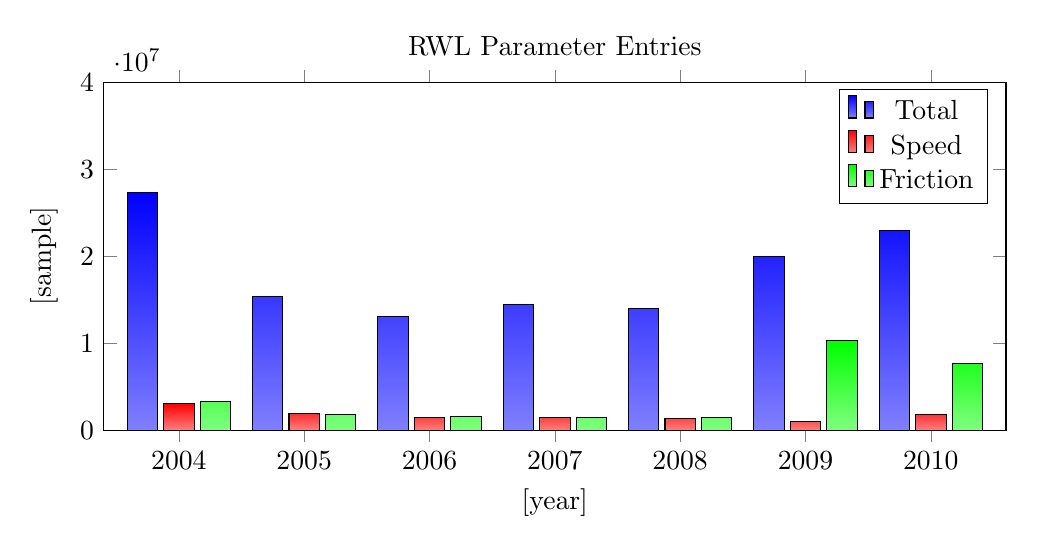
\begin{tikzpicture}
 
\begin{axis} [
	ybar,
	height=6cm,
	width=12cm,
	title={RWL Parameter Entries},
	ymin=0,
	xscale=1.1,
	ymax=4e7,
	xlabel={[year]},
	ylabel={[sample]},
symbolic x coords={$2004$, $2005$, $2006$, $2007$, $2008$, $2009$, $2010$}]

\addplot[
	top color=blue,
	bottom color=blue!50] coordinates {
($2004$, 27316136)
($2005$, 15313272)
($2006$, 13086456)
($2007$, 14410202)
($2008$, 14025183)
($2009$, 19913064)
($2010$, 22930278)
};
\addlegendentry{Total}

 \addplot[
 	top color=red,
 	bottom color=red!50] coordinates {
($2004$, 3020072)
($2005$, 1894684)
($2006$, 1483212)
($2007$, 1412812)
($2008$, 1365232)
($2009$, 1037740)
($2010$, 1747924)
};
\addlegendentry{Speed}

 \addplot[
 	top color=green,
 	bottom color=green!50] coordinates {
($2004$, 3256812)
($2005$, 1830160)
($2006$, 1540224)
($2007$, 1435680)
($2008$, 1402076)
($2009$, 10258132)
($2010$, 7622804)
};
\addlegendentry{Friction}

\end{axis}
 
\end{tikzpicture}

\caption{Total entries in blue and missing ones in red and green}
\label{f:rwa_missing_chart}
\end{figure}

For the unequal measurement periods, a second analysis is done in figure \ref{f:rwa_time_bin}. Here, the time-delta between single measurements is calculated and categorized into bins of 5 seconds. From there we can see again two things:

\begin{enumerate}
\item The measurements can be put into 3 major bins, one is that  less than 5 seconds, 15 to 20 seconds and more 30 seconds.
\item Roughly $\approx 70\%$ of the points fall into the \enquote{30 seconds or less} category and $\approx 99\%$ into the \enquote{5 minutes or less} category.
\end{enumerate}

\begin{figure}[htb]
\centering
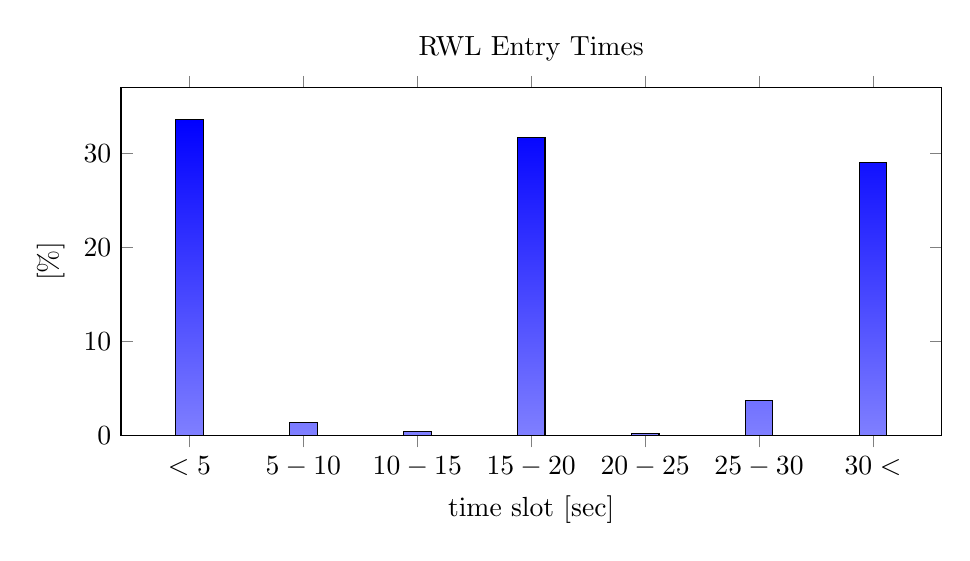
\begin{tikzpicture}
 
\begin{axis} [
	ybar,
	height=6cm,
	width=12cm,
	title={RWL Entry Times},
	ymin=0,
	xlabel={time slot [sec]},
	ylabel={[\%]},
	symbolic x coords={$< 5$, $5 - 10$, $10 - 15$, $15 - 20$, $20 - 25$, $25 - 30$, $30 <$}]
\addplot[
	top color=blue,
	bottom color=blue!50] coordinates {
    ($< 5$, 33.6) 
    ($5 - 10$, 1.4) 
    ($10 - 15$, 0.4) 
    ($15 - 20$, 31.7) 
    ($20 - 25$, 0.2) 
    ($25 - 30$, 3.7) 
    ($30 <$, 29.0)
};
\end{axis}
 
\end{tikzpicture}

\caption{Time bins for all the measurements}
\label{f:rwa_time_bin}
\end{figure}

As an example for one reaction wheel, the plot in figure \ref{f:rwa_example} shows the friction and speed of the \ac{rwa} B in the fourth quarter in 2008 right before the anomalies occurred. It can be seen that the friction follows the speed as expected, except where the wheel is rapidly accelerated. \newline
Another important detail to note for later is that one cycle of speed up/down takes at least $\SI{2e5}{\second}$ (respective 55 hours).

\begin{figure}[H]
\centering
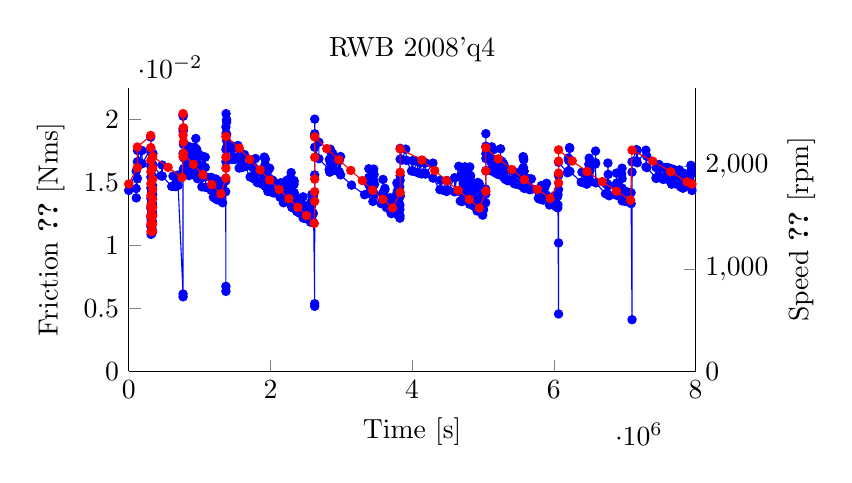
\begin{tikzpicture}
	\pgfplotsset{set layers}
	\begin{axis}[
		scale only axis,
		scale=0.9,
		xmin=0, xmax=8e6,
		ymin=0,
		height=4cm,
		width=8cm,
		title={RWB 2008'q4},
		axis y line*=left,
		axis x line*=bottom,
		xlabel={Time [s]},
		ylabel style = {align=center},
		ylabel={Friction \ref{eg:frict} [Nms]},
]
	\addplot[mark size=1.5pt, color=blue, mark=*] plot coordinates {		(0.0, 0.0143567)
		(105473.0, 0.0158838)
		(105665.0, 0.0145078)
		(106817.0, 0.0137635)
		(122433.0, 0.0153072)
		(122497.0, 0.0166348)
		(124801.0, 0.0175255)
		(147585.0, 0.0166073)
		(186049.0, 0.0175268)
		(190017.0, 0.0164748)
		(310209.0, 0.0176741)
		(310913.0, 0.0185882)
		(312129.0, 0.0174017)
		(312641.0, 0.0162766)
		(312961.0, 0.0154247)
		(313281.0, 0.0145622)
		(313473.0, 0.0137377)
		(313793.0, 0.0129257)
		(313985.0, 0.0122779)
		(314241.0, 0.0115059)
		(314817.0, 0.010873)
		(316417.0, 0.0114793)
		(316865.0, 0.0120837)
		(318465.0, 0.0130843)
		(318593.0, 0.0118921)
		(320257.0, 0.0133524)
		(320385.0, 0.0124064)
		(321921.0, 0.0115869)
		(321985.0, 0.0122657)
		(322049.0, 0.0132631)
		(322177.0, 0.0139334)
		(322241.0, 0.0122938)
		(323713.0, 0.0114778)
		(323777.0, 0.0124753)
		(323841.0, 0.0132169)
		(323969.0, 0.0140541)
		(324033.0, 0.0123579)
		(325121.0, 0.013381)
		(325441.0, 0.0123188)
		(325505.0, 0.0113349)
		(325569.0, 0.0126808)
		(325633.0, 0.0141395)
		(325697.0, 0.0153213)
		(325825.0, 0.0142726)
		(326273.0, 0.0133261)
		(326529.0, 0.0123428)
		(327297.0, 0.0110972)
		(327361.0, 0.0122326)
		(327425.0, 0.0132456)
		(327553.0, 0.0139787)
		(327617.0, 0.0123638)
		(329089.0, 0.0109556)
		(329153.0, 0.0123401)
		(329217.0, 0.0131999)
		(329345.0, 0.0139401)
		(329409.0, 0.0123701)
		(331585.0, 0.0133659)
		(333057.0, 0.0126659)
		(333761.0, 0.011869)
		(334209.0, 0.0111774)
		(335361.0, 0.0118739)
		(335873.0, 0.0125076)
		(336449.0, 0.0132096)
		(336897.0, 0.0140208)
		(337217.0, 0.0147384)
		(337857.0, 0.0154798)
		(338433.0, 0.0164134)
		(341825.0, 0.0172892)
		(342913.0, 0.0163373)
		(456321.0, 0.0155156)
		(472193.0, 0.0163727)
		(473665.0, 0.0154954)
		(606721.0, 0.014678)
		(624513.0, 0.0155013)
		(632065.0, 0.0146918)
		(660673.0, 0.0154574)
		(667073.0, 0.0146661)
		(694273.0, 0.0155752)
		(696961.0, 0.0147589)
		(766785.0, 0.00614051)
		(766849.0, 0.015856)
		(766913.0, 0.0172854)
		(766977.0, 0.00591318)
		(767041.0, 0.0190463)
		(767169.0, 0.0203415)
		(767489.0, 0.0192783)
		(768449.0, 0.0202423)
		(771073.0, 0.0192072)
		(773249.0, 0.0180062)
		(773633.0, 0.0169556)
		(774209.0, 0.0160943)
		(784833.0, 0.0169409)
		(785153.0, 0.016016)
		(813057.0, 0.0170904)
		(813185.0, 0.0161186)
		(826305.0, 0.0170338)
		(826433.0, 0.0159679)
		(829761.0, 0.0174117)
		(830529.0, 0.016424)
		(830593.0, 0.0172479)
		(840449.0, 0.0159552)
		(845121.0, 0.0178542)
		(846529.0, 0.0167253)
		(847745.0, 0.017629)
		(850945.0, 0.0164373)
		(851009.0, 0.0155333)
		(861185.0, 0.016366)
		(861697.0, 0.0173036)
		(871681.0, 0.0164029)
		(872449.0, 0.0173732)
		(927361.0, 0.0160451)
		(927617.0, 0.016941)
		(929537.0, 0.0177999)
		(929729.0, 0.0165243)
		(929793.0, 0.0175124)
		(930561.0, 0.0159927)
		(930753.0, 0.0170646)
		(946497.0, 0.0155172)
		(946689.0, 0.0174488)
		(946945.0, 0.0184811)
		(947265.0, 0.0175012)
		(947585.0, 0.0165818)
		(948481.0, 0.0174388)
		(948673.0, 0.0162594)
		(948801.0, 0.0172906)
		(949505.0, 0.0163614)
		(949633.0, 0.0173666)
		(953729.0, 0.0161751)
		(953793.0, 0.0175238)
		(956097.0, 0.0165092)
		(956225.0, 0.0174361)
		(958593.0, 0.016329)
		(958657.0, 0.0176279)
		(964929.0, 0.0157067)
		(965185.0, 0.0166205)
		(965505.0, 0.017452)
		(965633.0, 0.0163665)
		(965697.0, 0.017305)
		(969921.0, 0.0161361)
		(970241.0, 0.0152904)
		(974337.0, 0.017033)
		(983297.0, 0.015431)
		(1033089.0, 0.0146422)
		(1039425.0, 0.0153852)
		(1042305.0, 0.0162508)
		(1042369.0, 0.0170792)
		(1080129.0, 0.0161826)
		(1080193.0, 0.016998)
		(1086657.0, 0.0154406)
		(1086849.0, 0.0145905)
		(1162817.0, 0.015396)
		(1162881.0, 0.0143643)
		(1163457.0, 0.0153716)
		(1168641.0, 0.0145685)
		(1194689.0, 0.0138293)
		(1195777.0, 0.0145727)
		(1217665.0, 0.0137349)
		(1224321.0, 0.014444)
		(1230337.0, 0.0152649)
		(1231425.0, 0.014451)
		(1244929.0, 0.0136196)
		(1265025.0, 0.0143618)
		(1266689.0, 0.013626)
		(1278337.0, 0.0143431)
		(1283457.0, 0.0135674)
		(1294401.0, 0.0148272)
		(1294465.0, 0.0138244)
		(1324993.0, 0.0147012)
		(1325121.0, 0.0133822)
		(1325377.0, 0.0151193)
		(1368449.0, 0.0142593)
		(1368833.0, 0.0151179)
		(1371585.0, 0.00674677)
		(1371649.0, 0.0166372)
		(1371713.0, 0.0176176)
		(1371777.0, 0.00634724)
		(1371841.0, 0.0193921)
		(1373825.0, 0.0204517)
		(1374017.0, 0.0188907)
		(1381569.0, 0.0199695)
		(1381825.0, 0.0183037)
		(1382081.0, 0.0197934)
		(1382145.0, 0.0187901)
		(1384065.0, 0.0178096)
		(1397953.0, 0.0169186)
		(1430785.0, 0.0179524)
		(1437953.0, 0.0168954)
		(1443713.0, 0.0177505)
		(1444801.0, 0.0168423)
		(1447425.0, 0.0178651)
		(1448769.0, 0.0168823)
		(1450753.0, 0.0178262)
		(1454849.0, 0.0169253)
		(1455297.0, 0.0177864)
		(1458817.0, 0.0168407)
		(1461697.0, 0.0177305)
		(1468865.0, 0.0168289)
		(1469953.0, 0.0178102)
		(1475137.0, 0.0168861)
		(1477313.0, 0.0178412)
		(1479745.0, 0.0168962)
		(1484545.0, 0.0177554)
		(1485377.0, 0.016866)
		(1485953.0, 0.01774)
		(1486145.0, 0.0168359)
		(1488193.0, 0.0178086)
		(1493057.0, 0.0168256)
		(1538881.0, 0.0178968)
		(1538945.0, 0.0168462)
		(1542145.0, 0.0179168)
		(1546689.0, 0.0169954)
		(1557889.0, 0.0161364)
		(1591297.0, 0.0170224)
		(1593089.0, 0.0161683)
		(1594561.0, 0.0170388)
		(1596609.0, 0.0161854)
		(1622209.0, 0.0172256)
		(1628481.0, 0.0162982)
		(1635457.0, 0.0171777)
		(1642561.0, 0.0162562)
		(1713665.0, 0.0154233)
		(1741249.0, 0.0162742)
		(1743617.0, 0.0153945)
		(1745793.0, 0.0161867)
		(1759425.0, 0.0153409)
		(1760769.0, 0.0161806)
		(1762625.0, 0.015319)
		(1775361.0, 0.0161084)
		(1778433.0, 0.0152476)
		(1781249.0, 0.0160315)
		(1789377.0, 0.0168879)
		(1801345.0, 0.0158704)
		(1809985.0, 0.0150354)
		(1813377.0, 0.0158237)
		(1817857.0, 0.0149699)
		(1880833.0, 0.0157274)
		(1881793.0, 0.0148695)
		(1885185.0, 0.0156708)
		(1886017.0, 0.0148619)
		(1893633.0, 0.0158992)
		(1895233.0, 0.0150204)
		(1911553.0, 0.0159378)
		(1912705.0, 0.0149584)
		(1913153.0, 0.0161606)
		(1913281.0, 0.0170058)
		(1918657.0, 0.01566)
		(1922241.0, 0.014871)
		(1922561.0, 0.0162812)
		(1923265.0, 0.015423)
		(1924545.0, 0.016407)
		(1925313.0, 0.0153852)
		(1925505.0, 0.0168815)
		(1925569.0, 0.0158147)
		(1927297.0, 0.0168213)
		(1927489.0, 0.0154557)
		(1928129.0, 0.0146689)
		(1953665.0, 0.015544)
		(1956033.0, 0.0147309)
		(1956993.0, 0.0159512)
		(1957249.0, 0.0150523)
		(1958593.0, 0.0158365)
		(1958721.0, 0.0150425)
		(1964289.0, 0.0142797)
		(1969473.0, 0.0152286)
		(1970113.0, 0.0143426)
		(1970369.0, 0.0150624)
		(1971137.0, 0.0142802)
		(1972353.0, 0.0151608)
		(1985025.0, 0.0143364)
		(1987457.0, 0.0151675)
		(1988481.0, 0.0161204)
		(1991361.0, 0.0144605)
		(2024385.0, 0.0151973)
		(2025281.0, 0.0142515)
		(2025665.0, 0.0149947)
		(2026625.0, 0.0142083)
		(2035905.0, 0.0151196)
		(2036033.0, 0.0141874)
		(2042689.0, 0.0149777)
		(2043585.0, 0.014207)
		(2048449.0, 0.0150138)
		(2051649.0, 0.0141611)
		(2128577.0, 0.014915)
		(2130113.0, 0.0140925)
		(2133569.0, 0.0148768)
		(2135169.0, 0.013815)
		(2153409.0, 0.0149682)
		(2153857.0, 0.0141404)
		(2182209.0, 0.013385)
		(2182913.0, 0.014116)
		(2193217.0, 0.0134053)
		(2210369.0, 0.0147245)
		(2215169.0, 0.0139036)
		(2232129.0, 0.0151586)
		(2267777.0, 0.0143485)
		(2271105.0, 0.0150997)
		(2276737.0, 0.0134309)
		(2277313.0, 0.0145682)
		(2278145.0, 0.0153345)
		(2286017.0, 0.014188)
		(2286081.0, 0.0150612)
		(2289217.0, 0.0143047)
		(2289345.0, 0.0133194)
		(2289729.0, 0.0149333)
		(2292481.0, 0.0157727)
		(2293505.0, 0.0147862)
		(2301441.0, 0.0137393)
		(2302017.0, 0.0130143)
		(2308993.0, 0.0137108)
		(2309377.0, 0.0130003)
		(2311681.0, 0.0140621)
		(2311937.0, 0.0132589)
		(2324481.0, 0.0139869)
		(2325505.0, 0.0132378)
		(2325697.0, 0.0139494)
		(2325953.0, 0.0150408)
		(2328321.0, 0.0138217)
		(2328833.0, 0.0148636)
		(2331393.0, 0.0139981)
		(2331457.0, 0.0150339)
		(2331905.0, 0.0140008)
		(2332289.0, 0.0148288)
		(2332417.0, 0.0140033)
		(2333249.0, 0.013277)
		(2333633.0, 0.0151385)
		(2335169.0, 0.0141783)
		(2335809.0, 0.0131626)
		(2344961.0, 0.0139637)
		(2345089.0, 0.0129681)
		(2348865.0, 0.0136932)
		(2349505.0, 0.0128916)
		(2355073.0, 0.0135754)
		(2357953.0, 0.0128626)
		(2369857.0, 0.0135286)
		(2370625.0, 0.012761)
		(2371137.0, 0.0134058)
		(2373057.0, 0.0126812)
		(2375809.0, 0.0133351)
		(2391873.0, 0.01264)
		(2402561.0, 0.0133109)
		(2406209.0, 0.0125948)
		(2415297.0, 0.0132494)
		(2415425.0, 0.0125718)
		(2432577.0, 0.0132427)
		(2432705.0, 0.0125515)
		(2435713.0, 0.0132367)
		(2447681.0, 0.0125084)
		(2460097.0, 0.0138499)
		(2460353.0, 0.0128362)
		(2460865.0, 0.0121733)
		(2461697.0, 0.0128863)
		(2477633.0, 0.0122384)
		(2479937.0, 0.0128506)
		(2487681.0, 0.012137)
		(2487937.0, 0.0128307)
		(2489921.0, 0.0121363)
		(2491841.0, 0.012776)
		(2508673.0, 0.0121286)
		(2521153.0, 0.0129423)
		(2521537.0, 0.0121977)
		(2522369.0, 0.0129381)
		(2525569.0, 0.0121211)
		(2530369.0, 0.0131901)
		(2531265.0, 0.012486)
		(2563777.0, 0.0118454)
		(2566273.0, 0.0125395)
		(2574657.0, 0.0119018)
		(2581249.0, 0.0131606)
		(2581313.0, 0.0120464)
		(2581761.0, 0.0135353)
		(2581825.0, 0.0120604)
		(2582465.0, 0.0132361)
		(2584769.0, 0.0140395)
		(2586049.0, 0.0132709)
		(2586241.0, 0.0119495)
		(2600257.0, 0.0125766)
		(2600769.0, 0.011845)
		(2603905.0, 0.0125097)
		(2605953.0, 0.0118119)
		(2606081.0, 0.0139055)
		(2624385.0, 0.00536539)
		(2624449.0, 0.0155935)
		(2624577.0, 0.00516429)
		(2624641.0, 0.0177848)
		(2624705.0, 0.0187216)
		(2624769.0, 0.0200162)
		(2625217.0, 0.0188562)
		(2636737.0, 0.0169854)
		(2683841.0, 0.0181856)
		(2683969.0, 0.0168749)
		(2828993.0, 0.0160069)
		(2832769.0, 0.0168274)
		(2836417.0, 0.0158074)
		(2839489.0, 0.0167806)
		(2844097.0, 0.0176288)
		(2844417.0, 0.0165438)
		(2854401.0, 0.0173808)
		(2864001.0, 0.0164747)
		(2868161.0, 0.0173296)
		(2874369.0, 0.0163732)
		(2879297.0, 0.0172818)
		(2884481.0, 0.0160632)
		(2887233.0, 0.0170115)
		(2893121.0, 0.0159504)
		(2952193.0, 0.016796)
		(2954369.0, 0.0158805)
		(2970753.0, 0.0167183)
		(2971521.0, 0.0158306)
		(2989569.0, 0.0170479)
		(2990081.0, 0.0155896)
		(3144001.0, 0.0147789)
		(3327937.0, 0.0140171)
		(3388225.0, 0.0148089)
		(3388481.0, 0.0160769)
		(3388609.0, 0.014123)
		(3388865.0, 0.0153915)
		(3408193.0, 0.0143196)
		(3445953.0, 0.013485)
		(3446721.0, 0.0142463)
		(3457473.0, 0.0151447)
		(3457729.0, 0.0160536)
		(3460033.0, 0.0147905)
		(3462465.0, 0.0156312)
		(3468865.0, 0.0148483)
		(3469889.0, 0.0140496)
		(3561793.0, 0.0133109)
		(3588673.0, 0.0140975)
		(3588801.0, 0.0152289)
		(3588929.0, 0.0141641)
		(3589185.0, 0.0133949)
		(3615041.0, 0.01452)
		(3615105.0, 0.0136636)
		(3615297.0, 0.0144095)
		(3615489.0, 0.013682)
		(3636289.0, 0.0129974)
		(3670913.0, 0.0137265)
		(3672193.0, 0.0129616)
		(3691073.0, 0.0137781)
		(3692865.0, 0.0128297)
		(3693889.0, 0.0135825)
		(3695809.0, 0.0128642)
		(3700929.0, 0.0135139)
		(3703041.0, 0.0125657)
		(3703297.0, 0.0132527)
		(3707777.0, 0.0125195)
		(3710977.0, 0.0132778)
		(3715457.0, 0.0126138)
		(3716225.0, 0.0134684)
		(3717185.0, 0.0127259)
		(3783553.0, 0.0136093)
		(3783681.0, 0.0128817)
		(3785089.0, 0.0140584)
		(3785729.0, 0.014963)
		(3786241.0, 0.0141509)
		(3790145.0, 0.0148821)
		(3790849.0, 0.0133692)
		(3791553.0, 0.0143237)
		(3797057.0, 0.0133701)
		(3797121.0, 0.0124244)
		(3807809.0, 0.013422)
		(3811649.0, 0.0141993)
		(3811905.0, 0.0134198)
		(3811969.0, 0.0123597)
		(3815617.0, 0.0130657)
		(3823297.0, 0.0123268)
		(3823745.0, 0.0131502)
		(3824385.0, 0.0123292)
		(3824961.0, 0.0131944)
		(3825153.0, 0.0123876)
		(3825601.0, 0.0138968)
		(3825665.0, 0.0146312)
		(3826177.0, 0.0138398)
		(3826241.0, 0.0128511)
		(3827201.0, 0.0121568)
		(3830465.0, 0.0139618)
		(3830529.0, 0.0151599)
		(3830593.0, 0.0168412)
		(3830657.0, 0.0155361)
		(3830721.0, 0.0176996)
		(3857793.0, 0.0167654)
		(3909569.0, 0.0176343)
		(3920065.0, 0.0167465)
		(3990849.0, 0.015904)
		(4004417.0, 0.016721)
		(4020929.0, 0.0158678)
		(4063425.0, 0.0166827)
		(4088321.0, 0.0157421)
		(4116033.0, 0.0165368)
		(4132545.0, 0.0156644)
		(4183937.0, 0.0165615)
		(4184065.0, 0.0157322)
		(4187137.0, 0.0165341)
		(4187713.0, 0.0156543)
		(4293569.0, 0.0165273)
		(4293697.0, 0.0153363)
		(4391169.0, 0.014419)
		(4400001.0, 0.0151673)
		(4439041.0, 0.0143712)
		(4485697.0, 0.0151288)
		(4486145.0, 0.0142749)
		(4494273.0, 0.0151378)
		(4510913.0, 0.0143809)
		(4598593.0, 0.0153634)
		(4598657.0, 0.0142428)
		(4657089.0, 0.016275)
		(4669697.0, 0.0154083)
		(4670977.0, 0.0142607)
		(4679553.0, 0.0135181)
		(4698369.0, 0.0142442)
		(4702273.0, 0.0134725)
		(4718145.0, 0.0141496)
		(4720065.0, 0.0149121)
		(4726465.0, 0.0157278)
		(4733121.0, 0.0148706)
		(4733185.0, 0.015965)
		(4736897.0, 0.0149137)
		(4737025.0, 0.0136211)
		(4737537.0, 0.0145233)
		(4737793.0, 0.0137544)
		(4740353.0, 0.0150018)
		(4740609.0, 0.0141821)
		(4741185.0, 0.0149153)
		(4742465.0, 0.0156787)
		(4743745.0, 0.0147403)
		(4743873.0, 0.0161838)
		(4744641.0, 0.014565)
		(4745089.0, 0.0162315)
		(4745281.0, 0.0147097)
		(4746433.0, 0.0136625)
		(4810369.0, 0.0145426)
		(4810433.0, 0.0132654)
		(4810945.0, 0.0145212)
		(4811905.0, 0.0153325)
		(4813505.0, 0.0162226)
		(4813953.0, 0.0140397)
		(4814145.0, 0.0148472)
		(4814721.0, 0.0139954)
		(4815553.0, 0.0147134)
		(4820033.0, 0.0154541)
		(4820545.0, 0.0146613)
		(4823489.0, 0.0155409)
		(4826369.0, 0.0147266)
		(4827329.0, 0.0134529)
		(4844801.0, 0.0141616)
		(4844865.0, 0.0149798)
		(4846849.0, 0.013952)
		(4848705.0, 0.0132267)
		(4876225.0, 0.0141283)
		(4876353.0, 0.013088)
		(4916737.0, 0.0143059)
		(4916801.0, 0.0127257)
		(4916865.0, 0.0135222)
		(4917121.0, 0.0145504)
		(4925697.0, 0.0136487)
		(4925889.0, 0.0149892)
		(4926913.0, 0.014085)
		(4927041.0, 0.0130254)
		(4945345.0, 0.0140925)
		(4945409.0, 0.0149039)
		(4949441.0, 0.0136632)
		(4949505.0, 0.0146954)
		(4951425.0, 0.0132396)
		(4984577.0, 0.0125723)
		(4985281.0, 0.013218)
		(4987201.0, 0.0124781)
		(4987457.0, 0.0131547)
		(4995201.0, 0.0123955)
		(4995649.0, 0.0130394)
		(5007873.0, 0.0139785)
		(5007937.0, 0.0128328)
		(5035265.0, 0.0144774)
		(5037825.0, 0.0133779)
		(5038529.0, 0.0140621)
		(5040065.0, 0.0159355)
		(5040129.0, 0.0172652)
		(5040193.0, 0.0188626)
		(5040385.0, 0.0178625)
		(5040513.0, 0.0168836)
		(5097665.0, 0.0159658)
		(5105473.0, 0.0167786)
		(5114177.0, 0.0176429)
		(5114561.0, 0.0166916)
		(5122817.0, 0.0178183)
		(5122945.0, 0.0167812)
		(5123009.0, 0.0159052)
		(5132225.0, 0.016748)
		(5136513.0, 0.0158774)
		(5143809.0, 0.0166951)
		(5145665.0, 0.0175867)
		(5145793.0, 0.0166061)
		(5177537.0, 0.0157486)
		(5186817.0, 0.0165634)
		(5198145.0, 0.0156759)
		(5216449.0, 0.0165259)
		(5220993.0, 0.0156407)
		(5223745.0, 0.0164468)
		(5225985.0, 0.0156031)
		(5229057.0, 0.0164784)
		(5230017.0, 0.0156431)
		(5232065.0, 0.0167428)
		(5232513.0, 0.0158958)
		(5247617.0, 0.0167277)
		(5247873.0, 0.0176576)
		(5248513.0, 0.0167177)
		(5250497.0, 0.0158549)
		(5268737.0, 0.0166507)
		(5270785.0, 0.0156805)
		(5290049.0, 0.0164826)
		(5291777.0, 0.0154026)
		(5292929.0, 0.0162627)
		(5306369.0, 0.0154048)
		(5307969.0, 0.0162132)
		(5314753.0, 0.0152256)
		(5317441.0, 0.0160078)
		(5345345.0, 0.0152033)
		(5346497.0, 0.0159978)
		(5348417.0, 0.0151306)
		(5403457.0, 0.0159723)
		(5404609.0, 0.015101)
		(5419265.0, 0.0158701)
		(5421633.0, 0.0150682)
		(5438977.0, 0.0158365)
		(5439297.0, 0.0148919)
		(5468097.0, 0.0157473)
		(5469569.0, 0.0149589)
		(5470721.0, 0.0157091)
		(5470913.0, 0.0148534)
		(5534913.0, 0.015728)
		(5535425.0, 0.0147385)
		(5538305.0, 0.0155793)
		(5539969.0, 0.0147541)
		(5546881.0, 0.0157406)
		(5547393.0, 0.0148819)
		(5558017.0, 0.0160792)
		(5565761.0, 0.017039)
		(5570561.0, 0.016169)
		(5570881.0, 0.0169824)
		(5571073.0, 0.0157932)
		(5571137.0, 0.0148679)
		(5574529.0, 0.0167882)
		(5580673.0, 0.0158899)
		(5580801.0, 0.0145169)
		(5647937.0, 0.0152725)
		(5648257.0, 0.0144771)
		(5659777.0, 0.0152508)
		(5660545.0, 0.0144104)
		(5682625.0, 0.0152701)
		(5693889.0, 0.01447)
		(5780290.0, 0.0137429)
		(5788290.0, 0.0144672)
		(5797442.0, 0.0136751)
		(5799106.0, 0.014496)
		(5807874.0, 0.0137635)
		(5811074.0, 0.0145678)
		(5818242.0, 0.0138262)
		(5820162.0, 0.0145649)
		(5821634.0, 0.0138323)
		(5822914.0, 0.0147472)
		(5824130.0, 0.0137801)
		(5826242.0, 0.0144732)
		(5836354.0, 0.0137365)
		(5839810.0, 0.0144285)
		(5846210.0, 0.0135903)
		(5854466.0, 0.014438)
		(5856258.0, 0.0137095)
		(5869442.0, 0.0145642)
		(5871298.0, 0.0138031)
		(5871874.0, 0.0146084)
		(5872258.0, 0.0138108)
		(5872322.0, 0.0147134)
		(5873154.0, 0.0139412)
		(5896898.0, 0.0149234)
		(5896962.0, 0.0139788)
		(5937922.0, 0.0132017)
		(6016130.0, 0.0139648)
		(6016770.0, 0.0132584)
		(6026562.0, 0.013946)
		(6027522.0, 0.0131597)
		(6029506.0, 0.013875)
		(6030530.0, 0.0130589)
		(6032834.0, 0.0137792)
		(6033986.0, 0.013082)
		(6054466.0, 0.0138944)
		(6055042.0, 0.0129823)
		(6057090.0, 0.0140628)
		(6058050.0, 0.0132121)
		(6065986.0, 0.00455362)
		(6066050.0, 0.0144226)
		(6066114.0, 0.0155399)
		(6066178.0, 0.0101902)
		(6066242.0, 0.016588)
		(6191170.0, 0.015757)
		(6204610.0, 0.0169329)
		(6204738.0, 0.0159008)
		(6209218.0, 0.0167329)
		(6211138.0, 0.0158649)
		(6220226.0, 0.0177625)
		(6220354.0, 0.0168005)
		(6223938.0, 0.0176954)
		(6225602.0, 0.0167982)
		(6226498.0, 0.0158698)
		(6385986.0, 0.0150116)
		(6396226.0, 0.0158099)
		(6433218.0, 0.0149873)
		(6435394.0, 0.0157524)
		(6439234.0, 0.0149484)
		(6444610.0, 0.0158126)
		(6448578.0, 0.0149716)
		(6452930.0, 0.0157458)
		(6454466.0, 0.0149448)
		(6455362.0, 0.0157266)
		(6464450.0, 0.0148533)
		(6465346.0, 0.0156103)
		(6492354.0, 0.0164306)
		(6495938.0, 0.0155333)
		(6497858.0, 0.0169205)
		(6503234.0, 0.015022)
		(6509890.0, 0.0159328)
		(6510530.0, 0.0151219)
		(6585026.0, 0.0164488)
		(6587970.0, 0.0174836)
		(6588354.0, 0.0165571)
		(6591426.0, 0.0149614)
		(6727746.0, 0.014097)
		(6735170.0, 0.0148738)
		(6749890.0, 0.0141072)
		(6756290.0, 0.0148694)
		(6757570.0, 0.0140735)
		(6762562.0, 0.0165289)
		(6766530.0, 0.0156292)
		(6766786.0, 0.0147345)
		(6779330.0, 0.0139341)
		(6883266.0, 0.0147459)
		(6883522.0, 0.0157322)
		(6884674.0, 0.0147184)
		(6884802.0, 0.0139724)
		(6885698.0, 0.0149353)
		(6885826.0, 0.0141054)
		(6886594.0, 0.0148167)
		(6887490.0, 0.0140235)
		(6956482.0, 0.015658)
		(6960578.0, 0.0139873)
		(6961986.0, 0.0161233)
		(6963522.0, 0.0153047)
		(6963906.0, 0.0145333)
		(6964418.0, 0.0135281)
		(6997826.0, 0.0142987)
		(6998978.0, 0.0135111)
		(7030210.0, 0.0142485)
		(7030850.0, 0.0134772)
		(7089090.0, 0.0141788)
		(7090242.0, 0.0133106)
		(7102786.0, 0.00410043)
		(7102914.0, 0.0158109)
		(7103042.0, 0.0166278)
		(7164226.0, 0.0175963)
		(7164866.0, 0.0167055)
		(7175490.0, 0.0175507)
		(7176770.0, 0.0165542)
		(7298114.0, 0.0175528)
		(7299650.0, 0.0162205)
		(7311298.0, 0.017072)
		(7311682.0, 0.0161707)
		(7440706.0, 0.0153562)
		(7442754.0, 0.0161743)
		(7444802.0, 0.0153087)
		(7477186.0, 0.0163962)
		(7481410.0, 0.0155408)
		(7483202.0, 0.01641)
		(7484738.0, 0.0154704)
		(7485378.0, 0.0163689)
		(7486018.0, 0.0153851)
		(7489474.0, 0.0161689)
		(7544386.0, 0.0152263)
		(7548098.0, 0.0161637)
		(7581122.0, 0.0153537)
		(7584834.0, 0.0161859)
		(7591106.0, 0.0152848)
		(7608386.0, 0.0161695)
		(7620290.0, 0.0153169)
		(7628354.0, 0.0160871)
		(7629122.0, 0.0152613)
		(7630658.0, 0.0161147)
		(7632322.0, 0.0151944)
		(7636418.0, 0.0160342)
		(7637058.0, 0.0151446)
		(7637442.0, 0.0160669)
		(7642434.0, 0.015259)
		(7644354.0, 0.0160934)
		(7645762.0, 0.0151306)
		(7648322.0, 0.0159601)
		(7652290.0, 0.0149963)
		(7659970.0, 0.0157477)
		(7662402.0, 0.014853)
		(7670850.0, 0.0157448)
		(7676994.0, 0.0149572)
		(7683906.0, 0.015717)
		(7684930.0, 0.0149281)
		(7686850.0, 0.0160341)
		(7699522.0, 0.0150061)
		(7711554.0, 0.0157929)
		(7721026.0, 0.0148707)
		(7722178.0, 0.0158125)
		(7722562.0, 0.0149891)
		(7726786.0, 0.0157561)
		(7736258.0, 0.0149489)
		(7741378.0, 0.015843)
		(7751106.0, 0.0150436)
		(7772226.0, 0.0159872)
		(7774146.0, 0.0148267)
		(7781058.0, 0.0155946)
		(7789250.0, 0.0146412)
		(7820098.0, 0.0154212)
		(7820482.0, 0.0145342)
		(7828290.0, 0.0157277)
		(7829058.0, 0.0147427)
		(7831618.0, 0.0155496)
		(7837634.0, 0.0146158)
		(7919682.0, 0.0155507)
		(7923138.0, 0.0147013)
		(7928642.0, 0.0155544)
		(7933890.0, 0.0163501)
		(7934146.0, 0.0149988)
		(7936834.0, 0.0159326)
		(7942722.0, 0.0145464)
		(7948785.0, 0.0143567)
	};
\label{eg:frict}

\end{axis}
%
\begin{axis}[
		scale only axis,
		xmin=0, xmax=8e6,
		ymin=0,
		height=4cm,
		width=8cm,
		axis x line=none,
		ylabel style = {align=center},
		ylabel={Speed \ref{eg:speed} [rpm]},
		axis y line*=right,
		scale=0.9,
]
	\addplot[mark size=1.5pt, color=red, mark=*] plot coordinates {
		(0.0, 1830.79)
		(122369.0, 1990.85)
		(122497.0, 2192.58)
		(310209.0, 2305.39)
		(312321.0, 2186.48)
		(312641.0, 2060.98)
		(312897.0, 1950.2)
		(313153.0, 1833.33)
		(313409.0, 1720.53)
		(313665.0, 1615.35)
		(313921.0, 1518.8)
		(314177.0, 1440.55)
		(314497.0, 1367.38)
		(316481.0, 1435.98)
		(318273.0, 1533.54)
		(318401.0, 1626.52)
		(318529.0, 1527.44)
		(320129.0, 1604.17)
		(320385.0, 1506.61)
		(321921.0, 1604.67)
		(322177.0, 1514.23)
		(323713.0, 1606.71)
		(323969.0, 1521.34)
		(325505.0, 1609.25)
		(333121.0, 1524.9)
		(333569.0, 1443.6)
		(334081.0, 1368.39)
		(335489.0, 1439.02)
		(335873.0, 1522.36)
		(336193.0, 1601.63)
		(336513.0, 1684.96)
		(336897.0, 1780.49)
		(337281.0, 1876.02)
		(337729.0, 1986.79)
		(338177.0, 2100.1)
		(555905.0, 1994.41)
		(751873.0, 1894.31)
		(766785.0, 2098.07)
		(766913.0, 2309.45)
		(766977.0, 2518.8)
		(773249.0, 2380.59)
		(773633.0, 2244.41)
		(774081.0, 2130.59)
		(911937.0, 2023.88)
		(1044481.0, 1922.26)
		(1171649.0, 1825.71)
		(1300993.0, 1734.25)
		(1371585.0, 1889.23)
		(1371649.0, 1985.26)
		(1371713.0, 2094.51)
		(1371777.0, 2296.24)
		(1560385.0, 2181.4)
		(1705537.0, 2072.15)
		(1853761.0, 1968.5)
		(1988353.0, 1869.92)
		(2124545.0, 1776.42)
		(2260225.0, 1687.5)
		(2386305.0, 1602.64)
		(2507841.0, 1522.36)
		(2618753.0, 1446.14)
		(2624385.0, 1661.59)
		(2624449.0, 1755.59)
		(2624513.0, 1879.06)
		(2624577.0, 2091.97)
		(2624641.0, 2291.67)
		(2795201.0, 2176.83)
		(2965441.0, 2067.58)
		(3134657.0, 1963.41)
		(3296833.0, 1864.33)
		(3442241.0, 1770.83)
		(3586625.0, 1681.4)
		(3723905.0, 1597.05)
		(3830401.0, 1748.98)
		(3830465.0, 1945.63)
		(3830593.0, 2174.29)
		(4138689.0, 2065.55)
		(4318209.0, 1961.89)
		(4485249.0, 1863.31)
		(4648641.0, 1769.82)
		(4806593.0, 1680.89)
		(4950337.0, 1596.54)
		(5040001.0, 1760.67)
		(5040065.0, 1958.33)
		(5040193.0, 2186.48)
		(5214593.0, 2076.73)
		(5406913.0, 1972.56)
		(5584193.0, 1873.48)
		(5766721.0, 1779.47)
		(5946626.0, 1690.04)
		(6065986.0, 1841.46)
		(6066050.0, 1936.99)
		(6066114.0, 2053.86)
		(6066178.0, 2165.14)
		(6259266.0, 2056.4)
		(6467650.0, 1952.24)
		(6682690.0, 1854.17)
		(6882370.0, 1761.18)
		(7083074.0, 1672.76)
		(7103042.0, 2162.6)
		(7394882.0, 2054.37)
		(7648834.0, 1950.71)
		(7879234.0, 1852.13)
		(7948785.0, 1830.79)

	};
\label{eg:speed}
\end{axis}
\end{tikzpicture}

\caption{Data example from 2008'q4 reaction wheel B}
\label{f:rwa_example}
\end{figure}

\subsection{Solar Array}
The datasets of the solar array and power subsystem is a bit more complicated than the \ac{rwa}. In figure \ref{f:solar_array_block} the block diagram of the whole subsystem is shown. The datasets for the solar array include their display error, angular position, misalignment and incidence angle. Both arrays are mounted perpendicular to the xz-axis of the \ac{sc}, so in the positive-/negative direction of the y-axis. After the arrays follows the \ac{pcu} with parameters about voltage and current. For completeness, the \ac{plpdu} and \ac{sspdu} also contain information about voltage and current. \newline
Our main concern are the solar arrays themselves and the \ac{pcu}. The most important parameters for our analysis there are the voltage and current on the \ac{cm} and the misalignment of the arrays. The \acp{cm} are special solar cells within the solar array. They are operating in an open- and respective short-circuit mode to provide current and voltage information. This provides an estimate of the health state for the whole array. 

\begin{figure}[htb]
\centering
\input{2_DataMining/solar_array_block.pgf}
\caption{Solar array block diagram with the Solar Array Drive Mechanism (SADM), Power Control Unit (PCU) and following batteries as well as Power Distribution Units (PDU)}
\label{f:solar_array_block}
\end{figure}

As with the \ac{rwa} we will check the dataset for missing values and measurement periods.

Figure \ref{f:solar_missing_chart} shows the total number of possible entries for the parameters in blue. The total number of measurements is therefore less than the \ac{rwa}. Also the number of missing entries is substantially higher. In red, the \ac{cm} current and voltage are shown, they both have an equal amount of measurement points. The solar array misalignment entries are depicted in green. It can be seen, that especially the first year of service had the most measurements taken.

\begin{figure}[htb]
\centering
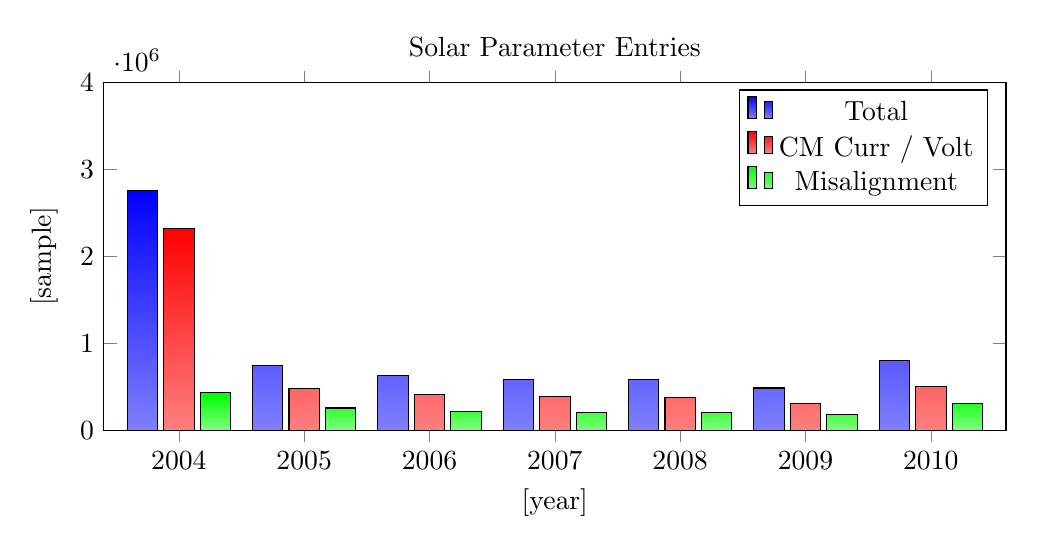
\begin{tikzpicture}
 
\begin{axis} [
	ybar,
	height=6cm,
	width=12cm,	
	title={Solar Parameter Entries},
	ymin=0,
	xscale=1.1,
	ymax=4e6,
	xlabel={[year]},
	ylabel={[sample]},
symbolic x coords={$2004$, $2005$, $2006$, $2007$, $2008$, $2009$, $2010$}]

\addplot[
	top color=blue,
	bottom color=blue!50] coordinates {
($2004$, 2756131)
($2005$, 741608)
($2006$, 630763)
($2007$, 586314)
($2008$, 581064)
($2009$, 486879)
($2010$, 804045)
};
\addlegendentry{Total}

 \addplot[
 	top color=red,
 	bottom color=red!50] coordinates {
($2004$, 2325175)
($2005$, 483706)
($2006$, 416720)
($2007$, 385541)
($2008$, 380300)
($2009$, 307714)
($2010$, 499781)
};
\addlegendentry{CM Curr / Volt}

 \addplot[
 	top color=green,
 	bottom color=green!50] coordinates {
($2004$, 431386)
($2005$, 257902)
($2006$, 214043)
($2007$, 200773)
($2008$, 200764)
($2009$, 179216)
($2010$, 304266)
};
\addlegendentry{Misalignment}

\end{axis}
 
\end{tikzpicture}

\caption{Total entries in blue and missing ones in red and green}
\label{f:solar_missing_chart}
\end{figure}

Again, for the unequal measurement periods, a second analysis is done in figure \ref{f:solar_time_bin}. The time distances between entries are similar to the \ac{rwa} and have their greatest percentages at \enquote{less than five seconds} ($\approx 29\%$), \enquote{15 to 20 seconds} ($\approx 41\%$) and \enquote{more than 30 seconds} with $\approx 21\%$. Again, 99\% of the measurements fall in the \enquote{5 minutes or less} category, which is later important for interpolation.

\begin{figure}[htb]
\centering
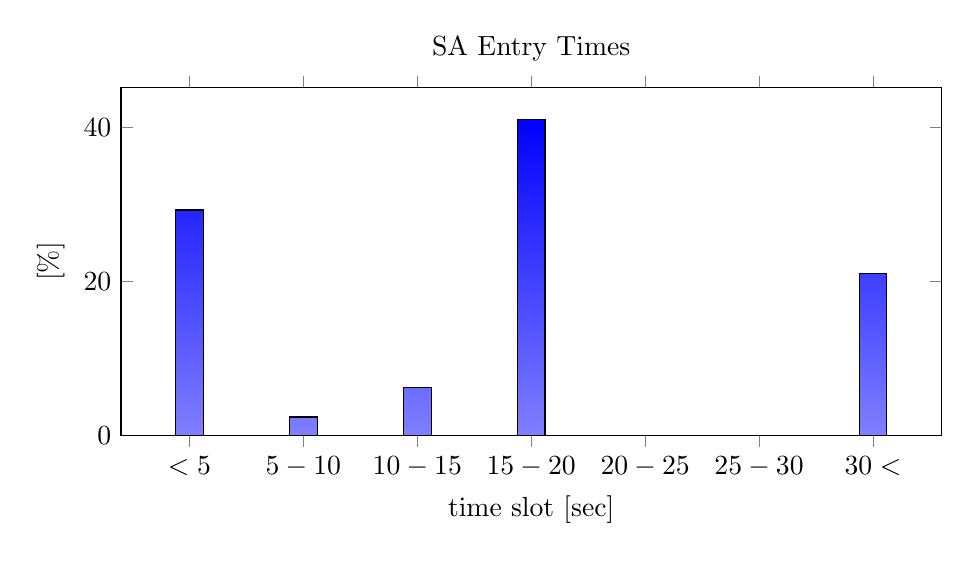
\begin{tikzpicture}
\begin{axis} [
	ybar,
	height=6cm,
	width=12cm,
	title={SA Entry Times},
	ymin=0,
	xlabel={time slot [sec]},
	ylabel={[\%]},
	symbolic x coords={$< 5$, $5 - 10$, $10 - 15$, $15 - 20$, $20 - 25$, $25 - 30$, $30 <$}]
\addplot[
	top color=blue,
	bottom color=blue!50] coordinates {
    ($< 5$, 29.3) 
    ($5 - 10$, 2.4) 
    ($10 - 15$, 6.2) 
    ($15 - 20$, 41.1) 
    ($20 - 25$, 0) 
    ($25 - 30$, 0) 
    ($30 <$, 21.1)
};
\end{axis}
\end{tikzpicture}

\caption{Time bins for all the measurements}
\label{f:solar_time_bin}
\end{figure}

As the solar arrays don't have any duty cycles like the reaction wheels, an overview on the operation over the whole time from 2004 till the end of 2010 is shown in figure \ref{f:solar_example}. If we look at the voltage in red, a trend can already be observed as the voltage continuously degrades over time, which is a well known effect of radiation \cite[p. 45f]{space-handbook}. The same holds true for the current in blue, except for a bump around $\SI{1.8e8}{\second}$ (respective year 2009). \newline
The decrease in voltage / current and therefore power can also be explained with Rosettas increasing distance from the sun over time.

\begin{figure}[H]
\centering
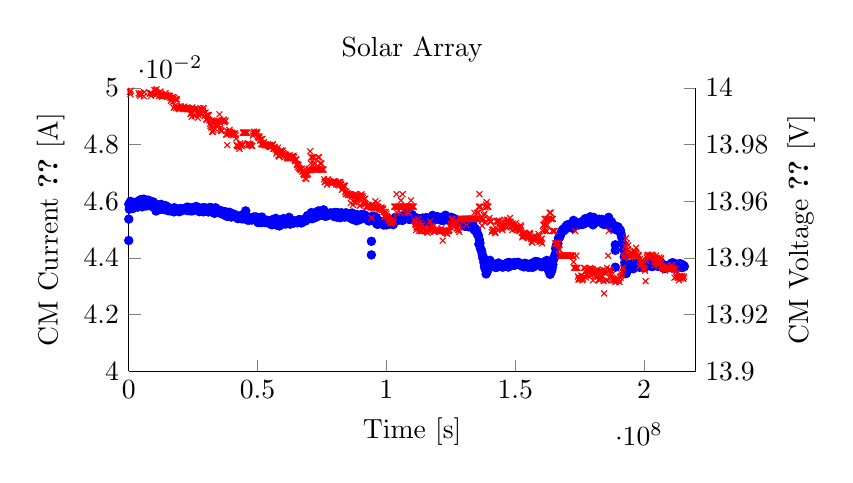
\begin{tikzpicture}
	\begin{axis}[
		scale only axis,
		xmin=0, xmax=2.2e8,
		ymin=0.04, ymax=0.05,
		height=4cm,
		width=8cm,
		title={Solar Array},
		axis y line*=left,
		axis x line*=bottom,
		xlabel={Time [s]},
		ylabel style = {align=center},
		ylabel={CM Current \ref{eg:amp} [A]},
		scale=0.9,
]
	\addplot[only marks, mark size=1.5pt, color=blue, mark=*] plot coordinates {
		(0.0, 0.0446150008849557)
		(32440.0, 0.0453708181818181)
		(33336.0, 0.0458941254545454)
		(249848.0, 0.0457204)
		(466232.0, 0.0457619107142857)
		(682232.0, 0.0459962232142857)
		(898217.0, 0.0458142839285714)
		(1114206.0, 0.0457821735905046)
		(1330217.0, 0.0458412107142857)
		(1546206.0, 0.0457406053412464)
		(1762217.0, 0.0458285982142857)
		(1978206.0, 0.0457940350148369)
		(2194217.0, 0.0457841401785714)
		(2410206.0, 0.0458480320474778)
		(2626217.0, 0.0459632964285714)
		(2842207.0, 0.0459315931750741)
		(3058218.0, 0.0458957375)
		(3274207.0, 0.0459392712166172)
		(3490218.0, 0.0457933241071428)
		(3706207.0, 0.0459867709876543)
		(3922218.0, 0.0459930151785714)
		(4138207.0, 0.0459722379821958)
		(4354218.0, 0.0460394125)
		(4570207.0, 0.0459902201780415)
		(4786218.0, 0.0460597169642857)
		(5002207.0, 0.0459750866468843)
		(5218207.0, 0.0458027083086055)
		(5434218.0, 0.0459815741071428)
		(5650233.0, 0.0458354517857142)
		(5866207.0, 0.0460751231454006)
		(6082218.0, 0.0459132544642857)
		(6298204.0, 0.0459331448071215)
		(6514204.0, 0.0459700275964391)
		(6730204.0, 0.0459205753709199)
		(6946219.0, 0.0458350142857142)
		(7162204.0, 0.0458829264094956)
		(7378219.0, 0.0458722080357143)
		(7594212.0, 0.0460393724550897)
		(7810302.0, 0.0458732923076923)
		(8026204.0, 0.045890061754386)
		(8242219.0, 0.0460066857142857)
		(8458299.0, 0.0459000071428571)
		(8674302.0, 0.0459764538461538)
		(8890299.0, 0.0458196285714285)
		(9106302.0, 0.0458640692307692)
		(9322299.0, 0.0459256642857142)
		(9538302.0, 0.0459764538461538)
		(9754299.0, 0.0458965857142857)
		(9970302.0, 0.045842)
		(10186299.0, 0.0459068285714285)
		(10402302.0, 0.0459009153846153)
		(10618300.0, 0.0456554071428571)
		(10834303.0, 0.0457664923076923)
		(11050300.0, 0.0458230499999999)
		(11266303.0, 0.0457020076923076)
		(11482300.0, 0.0457666)
		(11698303.0, 0.0457904153846153)
		(11914300.0, 0.0457135928571428)
		(12130303.0, 0.0458290846153846)
		(12346229.0, 0.0458871581818181)
		(12562292.0, 0.0457187142857142)
		(12778295.0, 0.0458806461538461)
		(12994292.0, 0.0457990857142857)
		(13210295.0, 0.0458033076923076)
		(13426293.0, 0.0458179214285714)
		(13642296.0, 0.045807)
		(13858293.0, 0.0457033285714285)
		(14074296.0, 0.0457830538461538)
		(14290293.0, 0.0458469928571428)
		(14506296.0, 0.0457056846153846)
		(14722293.0, 0.0458076428571428)
		(14938296.0, 0.0456946307692307)
		(15154293.0, 0.0457392428571428)
		(15370296.0, 0.0456651461538461)
		(15586293.0, 0.0457631714285714)
		(15802296.0, 0.0456946307692307)
		(16018293.0, 0.0457597571428571)
		(16234296.0, 0.0456633153846153)
		(16450232.0, 0.0456877581818181)
		(16666213.0, 0.0457051708333333)
		(16882232.0, 0.0456960363636363)
		(17098213.0, 0.0456977559523809)
		(17314232.0, 0.0457408927272727)
		(17530314.0, 0.0456246)
		(17746232.0, 0.0457713636363636)
		(17962213.0, 0.0457335333333333)
		(18178232.0, 0.0457043145454545)
		(18394214.0, 0.0457201380952381)
		(18610233.0, 0.0456812327272727)
		(18826214.0, 0.0456817898809523)
		(19042233.0, 0.0456807981818181)
		(19258214.0, 0.0457248422619048)
		(19474214.0, 0.0456410238095237)
		(19690214.0, 0.0456324666666665)
		(19906294.0, 0.0457306714285714)
		(20122297.0, 0.0457314846153846)
		(20338294.0, 0.0457358142857142)
		(20554297.0, 0.0457259461538461)
		(20770294.0, 0.0456827928571428)
		(20986297.0, 0.0456964615384615)
		(21202294.0, 0.0457135928571428)
		(21418297.0, 0.0457001615384615)
		(21634294.0, 0.0457478)
		(21850297.0, 0.0457148923076923)
		(22066294.0, 0.0456981785714285)
		(22282297.0, 0.0457296153846153)
		(22498294.0, 0.0457597642857142)
		(22714297.0, 0.0457941)
		(22930294.0, 0.0456691)
		(23146298.0, 0.0457167461538461)
		(23362294.0, 0.0457717357142857)
		(23578298.0, 0.0457425461538461)
		(23794205.0, 0.0457768767857143)
		(24010298.0, 0.0456614769230769)
		(24226295.0, 0.0457306857142857)
		(24442298.0, 0.0456706692307692)
		(24658295.0, 0.0457289857142857)
		(24874298.0, 0.0456651538461538)
		(25090295.0, 0.0457717357142857)
		(25306298.0, 0.0457130461538461)
		(25522295.0, 0.04578885)
		(25738298.0, 0.0457241076923076)
		(25954295.0, 0.0457819999999999)
		(26170298.0, 0.0458125153846153)
		(26386295.0, 0.0458025285714285)
		(26602298.0, 0.0457370076923076)
		(26818295.0, 0.0456725214285714)
		(27034298.0, 0.0456762076923077)
		(27250295.0, 0.0457597714285714)
		(27466298.0, 0.0456338307692307)
		(27682295.0, 0.0456999)
		(27898298.0, 0.0457535769230769)
		(28114295.0, 0.04569305)
		(28330298.0, 0.0457148923076923)
		(28546295.0, 0.04572385)
		(28762298.0, 0.045772)
		(28978295.0, 0.0456263357142857)
		(29194298.0, 0.045755423076923)
		(29410296.0, 0.0457016142857142)
		(29626299.0, 0.0457683076923076)
		(29842296.0, 0.0457255642857142)
		(30058299.0, 0.0457167461538461)
		(30274296.0, 0.0456622642857142)
		(30490299.0, 0.0457406923076923)
		(30706296.0, 0.0456879214285714)
		(30922299.0, 0.0456227923076923)
		(31138296.0, 0.0457512142857142)
		(31354299.0, 0.0457793692307692)
		(31570296.0, 0.0456810857142857)
		(31786223.0, 0.0456678178571428)
		(32002296.0, 0.0457751428571428)
		(32218299.0, 0.0457388461538461)
		(32434296.0, 0.0457101571428571)
		(32650299.0, 0.0456062)
		(32866296.0, 0.0456143642857142)
		(33082299.0, 0.0456540999999999)
		(33298296.0, 0.0455733142857142)
		(33514299.0, 0.0456135769230769)
		(33730296.0, 0.0457700214285714)
		(33946299.0, 0.045672523076923)
		(34162296.0, 0.0457016)
		(34378299.0, 0.0456080615384615)
		(34594296.0, 0.0456177999999999)
		(34810299.0, 0.0456062153846153)
		(35026297.0, 0.0456554142857142)
		(35242297.0, 0.0456725285714285)
		(35458297.0, 0.0456434357142857)
		(35674300.0, 0.0456725307692307)
		(35890297.0, 0.0455698999999999)
		(36106300.0, 0.0456080384615384)
		(36322297.0, 0.0455476785714285)
		(36538297.0, 0.0455476785714285)
		(36754297.0, 0.0455545)
		(36970297.0, 0.0455408285714285)
		(37186297.0, 0.0455767357142857)
		(37402297.0, 0.0456348785714285)
		(37618297.0, 0.0456023785714285)
		(37834300.0, 0.0455804384615384)
		(38050297.0, 0.0454689928571428)
		(38266300.0, 0.045492023076923)
		(38482297.0, 0.0454741357142857)
		(38698300.0, 0.0454938538461538)
		(38914297.0, 0.04561265)
		(39130300.0, 0.0455546461538461)
		(39346297.0, 0.0455972571428571)
		(39562300.0, 0.0454791307692307)
		(39778297.0, 0.0454433428571428)
		(39994300.0, 0.0455399153846153)
		(40210297.0, 0.0454861071428571)
		(40426300.0, 0.0454791384615384)
		(40642297.0, 0.0455493857142857)
		(40858301.0, 0.0455251769230769)
		(41074298.0, 0.0455219999999999)
		(41290301.0, 0.0455215)
		(41506298.0, 0.0454843999999999)
		(41722301.0, 0.0454607153846153)
		(41938298.0, 0.0454946357142857)
		(42154301.0, 0.0454109692307692)
		(42370298.0, 0.0453868785714285)
		(42586301.0, 0.0454588538461538)
		(42802298.0, 0.0454159642857142)
		(43018301.0, 0.0454662384615384)
		(43234298.0, 0.0454655714285714)
		(43450301.0, 0.0454017461538461)
		(43666298.0, 0.0454108357142857)
		(43882301.0, 0.045422023076923)
		(44098298.0, 0.0453749214285714)
		(44314042.0, 0.0455289)
		(44530106.0, 0.0454211)
		(44746170.0, 0.04545705)
		(44962234.0, 0.0454331)
		(45178298.0, 0.045481)
		(45394874.0, 0.0456605499999999)
		(45610938.0, 0.04544505)
		(45827002.0, 0.04544505)
		(46043066.0, 0.0453373)
		(46259194.0, 0.0453749214285714)
		(46475197.0, 0.0453373076923077)
		(46691194.0, 0.0453441428571428)
		(46907198.0, 0.0453483461538461)
		(47123195.0, 0.0453595357142857)
		(47339198.0, 0.0454072692307692)
		(47555195.0, 0.0453749214285714)
		(47771198.0, 0.0453373076923077)
		(47987195.0, 0.0453971428571428)
		(48203198.0, 0.0453907153846153)
		(48419195.0, 0.0454313642857142)
		(48635198.0, 0.0454459769230769)
		(48851195.0, 0.0453646499999999)
		(49067198.0, 0.0453409846153846)
		(49283195.0, 0.0454433285714285)
		(49499198.0, 0.0453907076923076)
		(49715195.0, 0.0454364928571428)
		(49931198.0, 0.0453962153846153)
		(50147195.0, 0.0452500785714285)
		(50363198.0, 0.0454036153846153)
		(50579195.0, 0.0454040071428571)
		(50795198.0, 0.0453041461538461)
		(51011195.0, 0.0452552071428571)
		(51227198.0, 0.0454146615384615)
		(51443195.0, 0.04524835)
		(51659198.0, 0.0454441307692307)
		(51875195.0, 0.0452586357142857)
		(52091198.0, 0.0452820615384615)
		(52307195.0, 0.0453663785714285)
		(52523198.0, 0.0453575461538461)
		(52739195.0, 0.0452672)
		(52955199.0, 0.0453004769230769)
		(53171196.0, 0.0452500785714285)
		(53387199.0, 0.0452580999999999)
		(53603196.0, 0.0452928357142857)
		(53819199.0, 0.0453262615384615)
		(54035196.0, 0.0452688999999999)
		(54251199.0, 0.0452267846153846)
		(54467196.0, 0.0452500714285714)
		(54683199.0, 0.0452396769230769)
		(54899196.0, 0.0452979714285714)
		(55115199.0, 0.0452175615384615)
		(55331196.0, 0.0451884928571428)
		(55547199.0, 0.0451678384615384)
		(55763196.0, 0.0453509785714285)
		(55979199.0, 0.0452323153846153)
		(56195196.0, 0.0452175714285714)
		(56411199.0, 0.0453538692307692)
		(56627196.0, 0.0452449571428571)
		(56843199.0, 0.0453262461538461)
		(57059196.0, 0.0453954571428571)
		(57275199.0, 0.045167823076923)
		(57491196.0, 0.0451696571428571)
		(57707199.0, 0.0452101999999999)
		(57923195.0, 0.0453133642857142)
		(58139198.0, 0.0453244153846153)
		(58355195.0, 0.0451320428571428)
		(58571198.0, 0.0451383769230769)
		(58787195.0, 0.0453441357142857)
		(59003198.0, 0.045167823076923)
		(59219195.0, 0.0453287428571428)
		(59435199.0, 0.0452102076923076)
		(59651196.0, 0.0452073214285714)
		(59867199.0, 0.0452452076923076)
		(60083196.0, 0.0453886071428571)
		(60299199.0, 0.0452433538461538)
		(60515196.0, 0.0452380928571428)
		(60731199.0, 0.045201)
		(60947196.0, 0.0452107285714285)
		(61163199.0, 0.0452101999999999)
		(61379196.0, 0.0453595357142857)
		(61595199.0, 0.0452175846153846)
		(61811196.0, 0.0453766357142857)
		(62027199.0, 0.0453778153846153)
		(62243196.0, 0.0454330785714285)
		(62459199.0, 0.045241523076923)
		(62675196.0, 0.0451936285714285)
		(62891199.0, 0.045241523076923)
		(63107196.0, 0.0453441357142857)
		(63323199.0, 0.0452525769230769)
		(63539196.0, 0.0453082214285714)
		(63755199.0, 0.0452783692307692)
		(63971196.0, 0.0452312571428571)
		(64187199.0, 0.0452783692307692)
		(64403196.0, 0.0452466642857142)
		(64619199.0, 0.0452728538461538)
		(64835196.0, 0.0453065285714285)
		(65051199.0, 0.0452912692307692)
		(65267196.0, 0.0452671785714285)
		(65483200.0, 0.045241523076923)
		(65699197.0, 0.0452552)
		(65915200.0, 0.0452838846153846)
		(66131197.0, 0.0453544)
		(66347200.0, 0.0453391384615384)
		(66563197.0, 0.0453253214285714)
		(66779200.0, 0.0453225769230769)
		(66995197.0, 0.0452329642857142)
		(67211200.0, 0.0453373076923077)
		(67427197.0, 0.0453013857142857)
		(67643200.0, 0.0452746846153846)
		(67859197.0, 0.0453526857142857)
		(68075200.0, 0.0453115076923077)
		(68291197.0, 0.04532705)
		(68507200.0, 0.0453446538461538)
		(68723197.0, 0.0453099428571428)
		(68939200.0, 0.0454165076923076)
		(69155197.0, 0.0454091357142857)
		(69371200.0, 0.0454938692307692)
		(69587197.0, 0.0454313571428571)
		(69803200.0, 0.0454478076923076)
		(70019197.0, 0.0453988785714285)
		(70235069.0, 0.0454689999999999)
		(70451133.0, 0.0455289)
		(70667197.0, 0.0455049)
		(70883773.0, 0.0456007)
		(71099837.0, 0.0453852)
		(71315902.0, 0.0455528)
		(71531966.0, 0.04543305)
		(71748030.0, 0.0455289)
		(71964094.0, 0.0454091)
		(72180670.0, 0.0455169)
		(72396734.0, 0.0455886999999999)
		(72612798.0, 0.04556475)
		(72828862.0, 0.04544505)
		(73044926.0, 0.0456246)
		(73260990.0, 0.0455528)
		(73477566.0, 0.04548095)
		(73693630.0, 0.0456605499999999)
		(73909694.0, 0.0455169)
		(74125758.0, 0.04556475)
		(74341822.0, 0.0456486)
		(74557886.0, 0.0456246)
		(74774462.0, 0.0455049)
		(74990526.0, 0.0455648)
		(75206590.0, 0.0456246)
		(75422654.0, 0.0456006999999999)
		(75638718.0, 0.0456965)
		(75854785.0, 0.0455380769230769)
		(76070782.0, 0.0454843928571428)
		(76286785.0, 0.0454754538461538)
		(76502782.0, 0.0454878142857142)
		(76718785.0, 0.0455527999999999)
		(76934782.0, 0.0454826928571428)
		(77150786.0, 0.0455454384615384)
		(77366783.0, 0.0455083499999999)
		(77582786.0, 0.0455159615384615)
		(77798783.0, 0.0455579285714285)
		(78014786.0, 0.0455822538461538)
		(78230783.0, 0.0455784571428571)
		(78446786.0, 0.0455656846153846)
		(78662783.0, 0.0455852785714285)
		(78878786.0, 0.0455601615384615)
		(79094783.0, 0.0455579357142857)
		(79310786.0, 0.0455527999999999)
		(79526783.0, 0.0455887142857142)
		(79742786.0, 0.0454588692307692)
		(79958783.0, 0.0454997857142857)
		(80174786.0, 0.0456043615384615)
		(80390783.0, 0.0455134785714285)
		(80606786.0, 0.0455067692307692)
		(80822783.0, 0.0454381928571428)
		(81038786.0, 0.0456025307692307)
		(81254783.0, 0.0455151857142857)
		(81470786.0, 0.0455288692307692)
		(81686783.0, 0.0454553142857142)
		(81902786.0, 0.0454625461538461)
		(82118783.0, 0.0454193928571428)
		(82334786.0, 0.045495723076923)
		(82550783.0, 0.0455955428571428)
		(82766786.0, 0.0455233538461538)
		(82982784.0, 0.045534)
		(83198787.0, 0.0455564769230769)
		(83414784.0, 0.0454655857142857)
		(83630787.0, 0.0454680769230769)
		(83846784.0, 0.0454416285714285)
		(84062787.0, 0.0455528076923076)
		(84278784.0, 0.0455921214285714)
		(84494787.0, 0.0455767461538461)
		(84710784.0, 0.0454912428571428)
		(84926787.0, 0.0455435846153846)
		(85142784.0, 0.0454399142857142)
		(85358787.0, 0.0455012307692307)
		(85574784.0, 0.0455647571428571)
		(85790787.0, 0.045549123076923)
		(86006784.0, 0.0455322857142857)
		(86222787.0, 0.0455362384615384)
		(86438784.0, 0.0455579428571428)
		(86654787.0, 0.0455859461538461)
		(86870784.0, 0.0453612428571428)
		(87086787.0, 0.0455177999999999)
		(87302784.0, 0.0454279499999999)
		(87518787.0, 0.0454717769230769)
		(87734784.0, 0.0454758357142857)
		(87950787.0, 0.0453851769230769)
		(88166784.0, 0.0454382142857142)
		(88382787.0, 0.0453096769230769)
		(88598785.0, 0.0455271285714285)
		(88814788.0, 0.0454220307692307)
		(89030785.0, 0.0454707071428571)
		(89246788.0, 0.0454349153846153)
		(89462785.0, 0.0454843857142857)
		(89678788.0, 0.0453520384615384)
		(89894785.0, 0.0455220142857142)
		(90110788.0, 0.0454864999999999)
		(90326785.0, 0.0454535999999999)
		(90542788.0, 0.0454772769230769)
		(90758785.0, 0.0455322857142857)
		(90974788.0, 0.0454846538461538)
		(91190785.0, 0.0454159785714285)
		(91406788.0, 0.0454349076923076)
		(91622785.0, 0.0455169071428571)
		(91838788.0, 0.0454073)
		(92054785.0, 0.0454724071428571)
		(92270788.0, 0.0454164923076923)
		(92486785.0, 0.0453561)
		(92702788.0, 0.0453999153846153)
		(92918785.0, 0.0453680857142857)
		(93134788.0, 0.0453078461538461)
		(93350785.0, 0.0453099499999999)
		(93566788.0, 0.0454109692307692)
		(93782785.0, 0.0454348)
		(93998788.0, 0.0453630769230769)
		(94179713.0, 0.0441075214285714)
		(94180609.0, 0.0445881571428571)
		(94181505.0, 0.0453458499999999)
		(94397509.0, 0.0453336076923076)
		(94613506.0, 0.0453971499999999)
		(94829509.0, 0.045479123076923)
		(95045506.0, 0.0453013785714285)
		(95261509.0, 0.0453594)
		(95477506.0, 0.0453219142857142)
		(95693509.0, 0.0453851846153846)
		(95909506.0, 0.0453629357142857)
		(96125509.0, 0.0454275461538461)
		(96341506.0, 0.0451919214285714)
		(96557509.0, 0.045232323076923)
		(96773506.0, 0.0451936214285714)
		(96989509.0, 0.045285723076923)
		(97205506.0, 0.0452363928571428)
		(97421509.0, 0.0452783692307692)
		(97637506.0, 0.0452244214285714)
		(97853509.0, 0.0452599384615384)
		(98069506.0, 0.0452209999999999)
		(98285509.0, 0.0452783846153846)
		(98501506.0, 0.0452363857142857)
		(98717509.0, 0.0452544153846153)
		(98933506.0, 0.0451611142857142)
		(99149509.0, 0.0452581)
		(99365506.0, 0.0452209928571428)
		(99581509.0, 0.045298623076923)
		(99797506.0, 0.0453014071428571)
		(100013510.0, 0.0451641461538461)
		(100229506.0, 0.0452757357142857)
		(100445510.0, 0.0452009999999999)
		(100661507.0, 0.04524495)
		(100877510.0, 0.045289423076923)
		(101093507.0, 0.0452004714285714)
		(101309510.0, 0.0452691692307692)
		(101525507.0, 0.0452073142857142)
		(101741510.0, 0.0452562538461538)
		(101957507.0, 0.0452877142857142)
		(102173510.0, 0.0452931076923076)
		(102389507.0, 0.0452415214285714)
		(102605510.0, 0.0451770461538461)
		(102821507.0, 0.0452193)
		(103037379.0, 0.0453492499999999)
		(103253443.0, 0.0453852)
		(103469507.0, 0.0454331)
		(103686083.0, 0.0453492499999999)
		(103902147.0, 0.04539715)
		(104118211.0, 0.0453732)
		(104334275.0, 0.04532535)
		(104550339.0, 0.0454331)
		(104766403.0, 0.0453373)
		(104982979.0, 0.04539715)
		(105199043.0, 0.0453612)
		(105415107.0, 0.04538515)
		(105631171.0, 0.0453732)
		(105847235.0, 0.0453373)
		(106063299.0, 0.045481)
		(106279876.0, 0.0453253)
		(106495940.0, 0.04544505)
		(106712004.0, 0.0454091)
		(106928068.0, 0.0454689999999999)
		(107144132.0, 0.0454331)
		(107360196.0, 0.045457)
		(107576772.0, 0.04549295)
		(107792836.0, 0.0454091)
		(108008900.0, 0.04556475)
		(108224964.0, 0.04556475)
		(108441028.0, 0.045457)
		(108657092.0, 0.045481)
		(108873668.0, 0.04536125)
		(109089732.0, 0.04536125)
		(109305796.0, 0.04550495)
		(109521860.0, 0.04550495)
		(109737924.0, 0.0455289)
		(109953988.0, 0.0455289)
		(110170564.0, 0.04543305)
		(110386628.0, 0.045457)
		(110602692.0, 0.04545705)
		(110818887.0, 0.0453501846153846)
		(111034884.0, 0.0453475428571428)
		(111250888.0, 0.0453630615384615)
		(111466885.0, 0.0453133571428571)
		(111682888.0, 0.0452544307692307)
		(111898885.0, 0.0454057142857142)
		(112114888.0, 0.0452728384615384)
		(112330885.0, 0.0452517928571428)
		(112546888.0, 0.0452231)
		(112762885.0, 0.0453834857142857)
		(112978888.0, 0.0453667769230769)
		(113194885.0, 0.0453270285714285)
		(113410888.0, 0.0453888769230769)
		(113626885.0, 0.0452894214285714)
		(113842888.0, 0.0452875846153846)
		(114058885.0, 0.0454074214285714)
		(114274888.0, 0.0452949461538461)
		(114490885.0, 0.0453150714285714)
		(114706888.0, 0.045333623076923)
		(114922885.0, 0.0453355928571428)
		(115138888.0, 0.0452709923076923)
		(115354885.0, 0.0454211142857142)
		(115570888.0, 0.0453870307692307)
		(115786885.0, 0.0454022928571428)
		(116002888.0, 0.0453943999999999)
		(116218885.0, 0.04539715)
		(116434888.0, 0.0452323)
		(116650885.0, 0.0453578214285714)
		(116866889.0, 0.0453465153846153)
		(117082886.0, 0.0453680714285714)
		(117298889.0, 0.0454146615384615)
		(117514886.0, 0.0453595428571428)
		(117730889.0, 0.0454054461538461)
		(117946886.0, 0.0455014999999999)
		(118162889.0, 0.0454220153846153)
		(118378886.0, 0.0453886214285714)
		(118594889.0, 0.0454275538461538)
		(118810886.0, 0.0453424214285714)
		(119026889.0, 0.0454054307692307)
		(119242886.0, 0.0454536071428571)
		(119458889.0, 0.0454072846153846)
		(119674886.0, 0.0454433357142857)
		(119890889.0, 0.0454515076923076)
		(120106886.0, 0.0454296428571428)
		(120322889.0, 0.0453814999999999)
		(120538886.0, 0.0453817571428571)
		(120754889.0, 0.0454146615384615)
		(120970886.0, 0.0454313642857142)
		(121186889.0, 0.0453280846153846)
		(121402886.0, 0.0453526928571428)
		(121618889.0, 0.0453336153846153)
		(121834886.0, 0.0454091285714285)
		(122050889.0, 0.0453336153846153)
		(122266886.0, 0.0454228142857142)
		(122482890.0, 0.0453501769230769)
		(122698887.0, 0.0453390214285714)
		(122914890.0, 0.0455067692307692)
		(123130887.0, 0.0454176785714285)
		(123346890.0, 0.0453907076923076)
		(123562887.0, 0.0453937357142857)
		(123778890.0, 0.0453465076923076)
		(123994887.0, 0.0454005785714285)
		(124210890.0, 0.0453373)
		(124426887.0, 0.0454159785714285)
		(124642890.0, 0.0453594076923076)
		(124858887.0, 0.0453031)
		(125074890.0, 0.0454349307692307)
		(125290887.0, 0.0453099571428571)
		(125506890.0, 0.0453022999999999)
		(125722887.0, 0.0453663785714285)
		(125938890.0, 0.0452967923076923)
		(126154887.0, 0.0453971571428571)
		(126370890.0, 0.0453575538461538)
		(126586887.0, 0.0452740142857142)
		(126802890.0, 0.0452452)
		(127018887.0, 0.0452996928571428)
		(127234890.0, 0.0452820538461538)
		(127450887.0, 0.0453407285714285)
		(127666890.0, 0.0453023153846153)
		(127882888.0, 0.0453099357142857)
		(128098891.0, 0.0453041384615384)
		(128314888.0, 0.0453082357142857)
		(128530888.0, 0.0453134)
		(128747464.0, 0.0452535)
		(128963528.0, 0.04530135)
		(129179592.0, 0.0452894)
		(129395656.0, 0.0452655)
		(129611720.0, 0.0452415)
		(129827784.0, 0.0453134)
		(130044360.0, 0.04522955)
		(130260424.0, 0.0451218)
		(130476488.0, 0.04519365)
		(130692552.0, 0.0452056)
		(130908616.0, 0.0451218)
		(131124680.0, 0.0452894)
		(131341256.0, 0.04518165)
		(131557320.0, 0.0451457)
		(131773384.0, 0.0451457)
		(131989448.0, 0.0450978499999999)
		(132205512.0, 0.0453373)
		(132421576.0, 0.0451697)
		(132638152.0, 0.04518165)
		(132854216.0, 0.0451457)
		(133070280.0, 0.0451936)
		(133286344.0, 0.0451098)
		(133502408.0, 0.0451936)
		(133718473.0, 0.0450978)
		(133935049.0, 0.04501405)
		(134151113.0, 0.04504995)
		(134367177.0, 0.04496615)
		(134583241.0, 0.045026)
		(134799305.0, 0.0449542)
		(135015369.0, 0.0449781)
		(135231945.0, 0.04485835)
		(135448009.0, 0.04482245)
		(135664073.0, 0.0447985)
		(135880137.0, 0.04448725)
		(136096201.0, 0.0446429)
		(136312265.0, 0.0445232)
		(136528841.0, 0.0443316)
		(136745225.0, 0.04428715)
		(136961225.0, 0.0442306857142857)
		(137177225.0, 0.0441263428571428)
		(137393225.0, 0.0440032071428571)
		(137609225.0, 0.0440374142857142)
		(137825225.0, 0.0438389928571428)
		(138041225.0, 0.0437175785714285)
		(138257225.0, 0.0436286357142857)
		(138473225.0, 0.0436303285714285)
		(138689225.0, 0.0434353571428571)
		(138905225.0, 0.0435807571428571)
		(139121225.0, 0.0435157571428571)
		(139337226.0, 0.0436149571428571)
		(139553226.0, 0.0437586142857142)
		(139769226.0, 0.0437090071428571)
		(139985226.0, 0.0438612428571428)
		(140201226.0, 0.0439159785714285)
		(140417226.0, 0.04372955)
		(140633226.0, 0.0437774428571428)
		(140849226.0, 0.0437723071428571)
		(141065226.0, 0.0437637642857142)
		(141281226.0, 0.0437346785714285)
		(141497226.0, 0.0437500714285714)
		(141713226.0, 0.0437774285714285)
		(141929226.0, 0.0437432285714285)
		(142145226.0, 0.0437124571428571)
		(142361226.0, 0.0436645357142857)
		(142577226.0, 0.0436713785714285)
		(142793226.0, 0.0437261285714285)
		(143009226.0, 0.0436850642857142)
		(143225226.0, 0.0436936285714285)
		(143441226.0, 0.0438236071428571)
		(143657226.0, 0.0437500785714285)
		(143873226.0, 0.0437552214285714)
		(144089226.0, 0.0437774571428571)
		(144305226.0, 0.0437329714285714)
		(144521226.0, 0.0437517857142857)
		(144737226.0, 0.0437363928571428)
		(144953227.0, 0.0436867785714285)
		(145169227.0, 0.0436765285714285)
		(145385227.0, 0.0437449571428571)
		(145601227.0, 0.0437124428571428)
		(145817227.0, 0.0437774357142857)
		(146033227.0, 0.0437757428571428)
		(146249227.0, 0.0437517928571428)
		(146465227.0, 0.0437158714285714)
		(146681227.0, 0.0437398285714285)
		(146897227.0, 0.0437569071428571)
		(147113227.0, 0.0438372928571428)
		(147329227.0, 0.0436782357142857)
		(147545227.0, 0.0438013857142857)
		(147761227.0, 0.0438372857142857)
		(147977227.0, 0.0437620428571428)
		(148193227.0, 0.0437894071428571)
		(148409227.0, 0.0437551928571428)
		(148625227.0, 0.0437928357142857)
		(148841227.0, 0.0438150571428571)
		(149057227.0, 0.0437449428571428)
		(149273227.0, 0.0438030785714285)
		(149489227.0, 0.0438338857142857)
		(149705227.0, 0.0437398142857142)
		(149921227.0, 0.0437757142857142)
		(150137227.0, 0.0437945357142857)
		(150353227.0, 0.0438355857142857)
		(150569167.0, 0.0438355785714285)
		(150785164.0, 0.04381436)
		(151001167.0, 0.0437928357142857)
		(151217164.0, 0.0438447066666666)
		(151433167.0, 0.0437962499999999)
		(151649164.0, 0.0438016133333333)
		(151865167.0, 0.0437671785714285)
		(152081164.0, 0.0437505333333333)
		(152297167.0, 0.0437346928571428)
		(152513164.0, 0.0437680933333333)
		(152729227.0, 0.0437107357142857)
		(152945227.0, 0.0437227071428571)
		(153161227.0, 0.0437073214285714)
		(153377227.0, 0.0436833785714285)
		(153593227.0, 0.0438048071428571)
		(153809227.0, 0.0438082142857142)
		(154025227.0, 0.0437192928571428)
		(154241227.0, 0.0437192857142857)
		(154457227.0, 0.0437158642857142)
		(154673227.0, 0.0437808785714285)
		(154889227.0, 0.0437364071428571)
		(155105227.0, 0.0436696714285714)
		(155321227.0, 0.0436953428571428)
		(155537227.0, 0.0437244214285714)
		(155753227.0, 0.0437398071428571)
		(155969227.0, 0.0437928357142857)
		(156185167.0, 0.0437979499999999)
		(156401164.0, 0.04367072)
		(156617167.0, 0.0437227071428571)
		(156833164.0, 0.0436946466666666)
		(157049167.0, 0.0436799428571428)
		(157265164.0, 0.04375214)
		(157481167.0, 0.0437415285714285)
		(157697164.0, 0.0438734333333333)
		(157913167.0, 0.0437894142857142)
		(158129164.0, 0.04386226)
		(158345167.0, 0.0438253214285714)
		(158561164.0, 0.0437968066666666)
		(158777167.0, 0.0438646428571428)
		(158993164.0, 0.0438047999999999)
		(159209167.0, 0.0437671857142857)
		(159425164.0, 0.0437696933333333)
		(159641167.0, 0.0437363928571428)
		(159857164.0, 0.0437281733333333)
		(160073167.0, 0.0436953428571428)
		(160289164.0, 0.0437984199999999)
		(160505167.0, 0.04369705)
		(160720844.0, 0.0437689)
		(160936908.0, 0.0437689)
		(161152972.0, 0.0437808499999999)
		(161369036.0, 0.04386465)
		(161585100.0, 0.043733)
		(161801165.0, 0.0437569)
		(162017741.0, 0.04382875)
		(162233805.0, 0.0439125499999999)
		(162449869.0, 0.0437569)
		(162665933.0, 0.04379285)
		(162881997.0, 0.0435654)
		(163098061.0, 0.0436611)
		(163314637.0, 0.0434815499999999)
		(163530701.0, 0.04342165)
		(163746765.0, 0.0434695499999999)
		(163962829.0, 0.04352945)
		(164178893.0, 0.0435654)
		(164394957.0, 0.0436611)
		(164611533.0, 0.0437689)
		(164827597.0, 0.0439844)
		(165043661.0, 0.0439724499999999)
		(165259725.0, 0.04404425)
		(165475789.0, 0.04412805)
		(165691853.0, 0.0443316)
		(165908429.0, 0.0444154)
		(166124493.0, 0.04447525)
		(166340557.0, 0.0444274)
		(166556621.0, 0.0445112)
		(166772685.0, 0.0446908)
		(166988749.0, 0.0447147)
		(167204813.0, 0.0447387)
		(167421390.0, 0.0447746)
		(167637454.0, 0.04485835)
		(167853518.0, 0.0448823)
		(168069582.0, 0.0449302)
		(168285646.0, 0.0449781)
		(168501710.0, 0.0450021)
		(168718286.0, 0.04495415)
		(168934350.0, 0.0450379999999999)
		(169150414.0, 0.0449901)
		(169366478.0, 0.04501405)
		(169582542.0, 0.0450978)
		(169798606.0, 0.0450739)
		(170015182.0, 0.04513375)
		(170231246.0, 0.0451697)
		(170447310.0, 0.04512175)
		(170663374.0, 0.04513375)
		(170879438.0, 0.0451457)
		(171095502.0, 0.0451697)
		(171312078.0, 0.0451936)
		(171528142.0, 0.04514575)
		(171744206.0, 0.04516965)
		(171960270.0, 0.0451457)
		(172176334.0, 0.04505)
		(172392398.0, 0.0451457)
		(172608974.0, 0.04532535)
		(172825038.0, 0.04527745)
		(173041103.0, 0.04514575)
		(173257167.0, 0.0452655)
		(173473231.0, 0.0451457)
		(173689295.0, 0.0452176)
		(173905871.0, 0.04524155)
		(174121935.0, 0.04524155)
		(174338191.0, 0.0451560071428571)
		(174554194.0, 0.0452083461538461)
		(174770191.0, 0.0451867785714285)
		(174986191.0, 0.0452230923076923)
		(175202188.0, 0.0451799285714285)
		(175418191.0, 0.045241523076923)
		(175634188.0, 0.0452586428571428)
		(175850191.0, 0.045180723076923)
		(176066188.0, 0.0452415285714285)
		(176282191.0, 0.0453004692307692)
		(176498188.0, 0.0451936214285714)
		(176714191.0, 0.0452452076923076)
		(176930188.0, 0.04524495)
		(177146191.0, 0.0453851692307692)
		(177362188.0, 0.04524665)
		(177578191.0, 0.0452967846153846)
		(177794188.0, 0.0452757428571428)
		(178010191.0, 0.045254423076923)
		(178226188.0, 0.0453219071428571)
		(178442191.0, 0.0453428153846153)
		(178658188.0, 0.0453065285714285)
		(178874191.0, 0.0453133692307692)
		(179090188.0, 0.0454519071428571)
		(179306191.0, 0.0454127999999999)
		(179522188.0, 0.0453150714285714)
		(179738191.0, 0.0452580923076923)
		(179954188.0, 0.0454057071428571)
		(180170191.0, 0.0451678384615384)
		(180386188.0, 0.0454313642857142)
		(180602191.0, 0.045355723076923)
		(180818188.0, 0.0453082285714285)
		(181034197.0, 0.0453557153846153)
		(181250188.0, 0.0452723)
		(181466197.0, 0.0452636384615384)
		(181682188.0, 0.0452706071428571)
		(181898197.0, 0.0452931)
		(182114188.0, 0.0453150785714285)
		(182330197.0, 0.0453262538461538)
		(182546188.0, 0.0453663642857142)
		(182762197.0, 0.0453299384615384)
		(182978188.0, 0.0453390071428571)
		(183194197.0, 0.0453446692307692)
		(183410188.0, 0.0452911142857142)
		(183626197.0, 0.0453612461538461)
		(183842188.0, 0.0452586285714285)
		(184058197.0, 0.045193623076923)
		(184274108.0, 0.0453279017857142)
		(184490197.0, 0.0452065307692307)
		(184706188.0, 0.0451885)
		(184922197.0, 0.0452286384615384)
		(185138188.0, 0.0452244142857142)
		(185354198.0, 0.0451825846153846)
		(185570188.0, 0.0453030928571428)
		(185786198.0, 0.045206523076923)
		(186002633.0, 0.0452655)
		(186239177.0, 0.0454331)
		(186498390.0, 0.0452375166666666)
		(186714125.0, 0.0452483642857142)
		(186930125.0, 0.0451918)
		(187146125.0, 0.0452244142857142)
		(187362125.0, 0.0452728384615384)
		(187578125.0, 0.0450704857142857)
		(187794125.0, 0.0451973153846153)
		(188010125.0, 0.0451559857142857)
		(188226125.0, 0.0450849461538461)
		(188442125.0, 0.0450226)
		(188658125.0, 0.045070223076923)
		(188831704.0, 0.0442688084444444)
		(188832608.0, 0.0436727848214284)
		(188834408.0, 0.0444650080357142)
		(188835308.0, 0.0450678089285714)
		(189051405.0, 0.0450568)
		(189267414.0, 0.0450923153846153)
		(189483405.0, 0.0449866857142857)
		(189699414.0, 0.0450996846153846)
		(189915405.0, 0.0450909999999999)
		(190131414.0, 0.0450426)
		(190347405.0, 0.0449422071428571)
		(190563414.0, 0.0449707615384615)
		(190779405.0, 0.0449798357142857)
		(190995414.0, 0.0448786615384615)
		(191211405.0, 0.0447728857142857)
		(191427414.0, 0.0446981461538461)
		(191643405.0, 0.0445094785714285)
		(191859414.0, 0.0444863384615384)
		(192075405.0, 0.0442888428571428)
		(192291414.0, 0.0440461076923076)
		(192507405.0, 0.0438424214285714)
		(192723414.0, 0.0436353538461538)
		(192939405.0, 0.0434456357142857)
		(193155414.0, 0.0434659076923076)
		(193371405.0, 0.0437073142857142)
		(193587414.0, 0.0437200846153846)
		(193803405.0, 0.0437363928571428)
		(194019414.0, 0.0437071769230769)
		(194235405.0, 0.0436252071428571)
		(194451414.0, 0.0437071846153846)
		(194667405.0, 0.0437757357142857)
		(194883414.0, 0.0437863769230769)
		(195099405.0, 0.0436850785714285)
		(195315414.0, 0.0437034923076923)
		(195531405.0, 0.0437364)
		(195747414.0, 0.0436187461538461)
		(195963405.0, 0.0436389071428571)
		(196179414.0, 0.0437955923076923)
		(196395405.0, 0.0437928214285714)
		(196611414.0, 0.0438140076923076)
		(196827405.0, 0.0437894)
		(197043414.0, 0.0438269)
		(197259405.0, 0.0437175714285714)
		(197475414.0, 0.0437237538461538)
		(197691405.0, 0.0436936285714285)
		(197907414.0, 0.043766123076923)
		(198123405.0, 0.0437175714285714)
		(198339414.0, 0.0436703307692307)
		(198555405.0, 0.0437859928571428)
		(198771414.0, 0.043814)
		(198987405.0, 0.0437192928571428)
		(199203414.0, 0.043734823076923)
		(199419405.0, 0.0437312642857142)
		(199635414.0, 0.0436777)
		(199851405.0, 0.0436594214285714)
		(200067415.0, 0.0437513923076923)
		(200283405.0, 0.0436628428571428)
		(200499415.0, 0.0436979692307692)
		(200715406.0, 0.0437124357142857)
		(200931415.0, 0.0437679692307692)
		(201147406.0, 0.0438783428571428)
		(201363415.0, 0.0438029384615384)
		(201579406.0, 0.0438167714285714)
		(201795415.0, 0.0438379538461538)
		(202011406.0, 0.0438441357142857)
		(202227415.0, 0.0437532384615384)
		(202443406.0, 0.0437124428571428)
		(202659415.0, 0.0437348153846153)
		(202875406.0, 0.043786)
		(203091415.0, 0.0438563692307692)
		(203307406.0, 0.0436970428571428)
		(203523415.0, 0.0438563615384615)
		(203739406.0, 0.0437962499999999)
		(203955415.0, 0.0437532307692307)
		(204171406.0, 0.0438338785714285)
		(204387415.0, 0.0439134692307692)
		(204603406.0, 0.04381335)
		(204819415.0, 0.0438066461538461)
		(205035406.0, 0.0438595142857142)
		(205251415.0, 0.0437735)
		(205467406.0, 0.0436987642857142)
		(205683415.0, 0.0438121769230769)
		(205899406.0, 0.0439039928571428)
		(206115415.0, 0.0438140076923076)
		(206331406.0, 0.0438577928571428)
		(206547415.0, 0.0437495307692307)
		(206763406.0, 0.0438013928571428)
		(206979415.0, 0.0437513846153846)
		(207195406.0, 0.0437073142857142)
		(207411415.0, 0.0437624384615384)
		(207627406.0, 0.0436457428571428)
		(207843415.0, 0.0436242769230769)
		(208059406.0, 0.0437346785714285)
		(208275415.0, 0.043721923076923)
		(208491406.0, 0.0437056)
		(208707415.0, 0.0436574307692307)
		(208923406.0, 0.0436748071428571)
		(209139415.0, 0.0436998153846153)
		(209355406.0, 0.0437175714285714)
		(209571415.0, 0.0436592923076923)
		(209787406.0, 0.0437227214285714)
		(210003415.0, 0.0437606076923076)
		(210219406.0, 0.0437227071428571)
		(210435415.0, 0.0437790153846153)
		(210651406.0, 0.0438082142857142)
		(210867415.0, 0.0438250615384615)
		(211083406.0, 0.0436867714285714)
		(211299415.0, 0.0438269)
		(211515406.0, 0.0437158642857142)
		(211731415.0, 0.0437919076923076)
		(211947406.0, 0.0436371785714285)
		(212163415.0, 0.0437384923076923)
		(212379406.0, 0.0437483642857142)
		(212595415.0, 0.0437827076923077)
		(212811406.0, 0.04372785)
		(213027415.0, 0.0437293)
		(213243406.0, 0.0436936357142857)
		(213459415.0, 0.0437476999999999)
		(213675406.0, 0.0437637571428571)
		(213891415.0, 0.0438029692307692)
		(214107406.0, 0.0437227071428571)
		(214323415.0, 0.0436758692307692)
		(214539406.0, 0.0436679714285714)
		(214755415.0, 0.0437679615384615)
		(214971406.0, 0.0436628428571428)
		(215187416.0, 0.0437071769230769)
		(215403407.0, 0.0437261357142857)
		(215619416.0, 0.0436979769230769)
	};
\label{eg:amp}
	\end{axis}

	\begin{axis}[
		scale only axis,
		xmin=0, xmax=2.2e8,
		ymin=13.9, ymax=14,
		height=4cm,
		width=8cm,
		axis x line=none,
		ylabel style = {align=center},
		ylabel={CM Voltage \ref{eg:volt} [V]},
		axis y line*=right,
		scale=0.9,
]
	\addplot[only marks, mark size=1.5pt, color=red, mark=x] plot coordinates {
		(0.0, 14.00842831858408)
		(216040.0, 14.001812727272725)
		(432008.0, 13.998601339285662)
		(648040.0, 13.99774727272728)
		(864006.0, 13.998986350148298)
		(1080016.0, 14.001192857142874)
		(1296006.0, 14.00155163204746)
		(1512016.0, 14.001577678571442)
		(1728006.0, 14.0013596439169)
		(1944016.0, 14.003039285714287)
		(2160006.0, 14.001653115726992)
		(2376016.0, 14.001769642857155)
		(2592006.0, 14.001437091988114)
		(2808017.0, 14.00173214285716)
		(3024007.0, 14.001500890207703)
		(3240017.0, 14.000924107142874)
		(3456007.0, 14.001360534124611)
		(3672017.0, 14.001308035714304)
		(3888007.0, 13.998144213649756)
		(4104017.0, 13.997621428571447)
		(4320007.0, 14.001372403560811)
		(4536017.0, 13.99723571428573)
		(4752007.0, 13.998028189910883)
		(4976471.0, 14.0015)
		(5193010.0, 14.00134642857144)
		(5409010.0, 14.001192857142872)
		(5625010.0, 14.000002678571445)
		(5841007.0, 13.99702508250816)
		(6057007.0, 13.998475964391607)
		(6273010.0, 14.000808928571448)
		(6489004.0, 14.00016023738869)
		(6705011.0, 14.000386607142874)
		(6921011.0, 14.001154464285731)
		(7137011.0, 14.000309821428589)
		(7353011.0, 14.001385714285734)
		(7569011.0, 14.001538392857157)
		(7785086.0, 14.001838461538457)
		(8001011.0, 14.000847321428584)
		(8217011.0, 13.997967857142871)
		(8433083.0, 13.998121428571425)
		(8649086.0, 13.997199999999994)
		(8865083.0, 13.998121428571425)
		(9081086.0, 14.000507692307687)
		(9297083.0, 14.001192857142852)
		(9513086.0, 14.001507692307689)
		(9729083.0, 14.001507142857138)
		(9945086.0, 13.99918461538461)
		(10161083.0, 13.99781428571428)
		(10377086.0, 13.99918461538461)
		(10593084.0, 13.997507142857136)
		(10809087.0, 13.99951538461538)
		(11025084.0, 14.001192857142852)
		(11241087.0, 13.997861538461532)
		(11457084.0, 13.998121428571425)
		(11673087.0, 13.998192307692303)
		(11889084.0, 13.997192857142853)
		(12105087.0, 13.997530769230764)
		(12321084.0, 13.99873571428571)
		(12537076.0, 13.99781428571428)
		(12753079.0, 13.997199999999994)
		(12969076.0, 13.99688571428571)
		(13185079.0, 13.997199999999994)
		(13401077.0, 13.997199999999994)
		(13617080.0, 13.997192307692302)
		(13833077.0, 13.997199999999994)
		(14049080.0, 13.997199999999994)
		(14265077.0, 13.998114285714282)
		(14481080.0, 13.997530769230764)
		(14697077.0, 13.997199999999994)
		(14913080.0, 13.996861538461532)
		(15129077.0, 13.997199999999994)
		(15345080.0, 13.997199999999994)
		(15561077.0, 13.997199999999994)
		(15777080.0, 13.996861538461532)
		(15993077.0, 13.997199999999994)
		(16209080.0, 13.99651538461538)
		(16425029.0, 13.995469642857149)
		(16641029.0, 13.99633571428572)
		(16857029.0, 13.996571428571436)
		(17073029.0, 13.995000000000005)
		(17289029.0, 13.99680714285715)
		(17505029.0, 13.99296071428571)
		(17721029.0, 13.996487500000004)
		(17937029.0, 13.993660714285708)
		(18153029.0, 13.996021428571437)
		(18369030.0, 13.992878571428562)
		(18585030.0, 13.996019642857148)
		(18801030.0, 13.995550000000003)
		(19017030.0, 13.99319285714285)
		(19233030.0, 13.992878571428564)
		(19449030.0, 13.99249285714285)
		(19665030.0, 13.99288035714285)
		(19881078.0, 13.992799999999995)
		(20097081.0, 13.99347692307692)
		(20313078.0, 13.993428571428568)
		(20529081.0, 13.992799999999995)
		(20745078.0, 13.992799999999995)
		(20961081.0, 13.99313846153846)
		(21177078.0, 13.992799999999995)
		(21393081.0, 13.992799999999995)
		(21609078.0, 13.993421428571423)
		(21825081.0, 13.992799999999995)
		(22041078.0, 13.992492857142851)
		(22257081.0, 13.99280769230769)
		(22473078.0, 13.992799999999995)
		(22689081.0, 13.992469230769228)
		(22905078.0, 13.992492857142851)
		(23121082.0, 13.99280769230769)
		(23337078.0, 13.992492857142851)
		(23553082.0, 13.992799999999995)
		(23769079.0, 13.992492857142851)
		(23985082.0, 13.99081538461538)
		(24201079.0, 13.99095714285714)
		(24417082.0, 13.989823076923074)
		(24633079.0, 13.993114285714285)
		(24849082.0, 13.992469230769228)
		(25065079.0, 13.992492857142851)
		(25281082.0, 13.992138461538458)
		(25497079.0, 13.992492857142851)
		(25713082.0, 13.990153846153843)
		(25929079.0, 13.99218571428571)
		(26145082.0, 13.99147692307692)
		(26361079.0, 13.992492857142851)
		(26577082.0, 13.99081538461538)
		(26793079.0, 13.989421428571424)
		(27009082.0, 13.990484615384611)
		(27225079.0, 13.991571428571424)
		(27441082.0, 13.99114615384615)
		(27657079.0, 13.990964285714282)
		(27873082.0, 13.992799999999995)
		(28089079.0, 13.992192857142854)
		(28305082.0, 13.99081538461538)
		(28521079.0, 13.992499999999996)
		(28737082.0, 13.99180769230769)
		(28953079.0, 13.992799999999995)
		(29169082.0, 13.992799999999995)
		(29385080.0, 13.99003571428571)
		(29601083.0, 13.99114615384615)
		(29817080.0, 13.991264285714282)
		(30033083.0, 13.988830769230766)
		(30249080.0, 13.990342857142853)
		(30465083.0, 13.988830769230766)
		(30681080.0, 13.990342857142853)
		(30897083.0, 13.990484615384611)
		(31113080.0, 13.990342857142853)
		(31329083.0, 13.988499999999997)
		(31545080.0, 13.987271428571423)
		(31761016.0, 13.986657142857142)
		(31977080.0, 13.986042857142852)
		(32193083.0, 13.988499999999997)
		(32409080.0, 13.984507142857138)
		(32625083.0, 13.984530769230766)
		(32841080.0, 13.985121428571423)
		(33057083.0, 13.988169230769229)
		(33273080.0, 13.98573571428571)
		(33489083.0, 13.98717692307692)
		(33705080.0, 13.988192857142852)
		(33921083.0, 13.98684615384615)
		(34137080.0, 13.98788571428571)
		(34353083.0, 13.988499999999997)
		(34569080.0, 13.987271428571423)
		(34785083.0, 13.98651538461538)
		(35001081.0, 13.988192857142852)
		(35217081.0, 13.990649999999995)
		(35433081.0, 13.98573571428571)
		(35649084.0, 13.985192307692303)
		(35865081.0, 13.98481428571428)
		(36081084.0, 13.984861538461534)
		(36297081.0, 13.988192857142852)
		(36513081.0, 13.988499999999997)
		(36729081.0, 13.988499999999997)
		(36945081.0, 13.98880714285714)
		(37161081.0, 13.98788571428571)
		(37377081.0, 13.988192857142852)
		(37593081.0, 13.988499999999997)
		(37809084.0, 13.983523076923072)
		(38025081.0, 13.983571428571423)
		(38241084.0, 13.979800000000004)
		(38457081.0, 13.984507142857138)
		(38673084.0, 13.983861538461534)
		(38889081.0, 13.984507142857138)
		(39105084.0, 13.985192307692303)
		(39321081.0, 13.984507142857138)
		(39537084.0, 13.984199999999996)
		(39753081.0, 13.983885714285709)
		(39969084.0, 13.983861538461536)
		(40185081.0, 13.984199999999996)
		(40401084.0, 13.983861538461534)
		(40617081.0, 13.98325714285714)
		(40833085.0, 13.983861538461536)
		(41049082.0, 13.98388571428571)
		(41265085.0, 13.983861538461536)
		(41481082.0, 13.983249999999998)
		(41697085.0, 13.982169230769232)
		(41913082.0, 13.979800000000004)
		(42129085.0, 13.979469230769231)
		(42345082.0, 13.97949285714286)
		(42561085.0, 13.979469230769231)
		(42777082.0, 13.979185714285718)
		(42993085.0, 13.978476923076926)
		(43209082.0, 13.980428571428574)
		(43425085.0, 13.979800000000004)
		(43641082.0, 13.979800000000004)
		(43857085.0, 13.979469230769231)
		(44073082.0, 13.980121428571431)
		(44288954.0, 13.9842)
		(44505018.0, 13.9842)
		(44721082.0, 13.9842)
		(44937658.0, 13.9842)
		(45153722.0, 13.9842)
		(45369786.0, 13.9842)
		(45585850.0, 13.9842)
		(45801914.0, 13.9842)
		(46017978.0, 13.9842)
		(46233978.0, 13.980428571428574)
		(46449981.0, 13.979800000000004)
		(46665978.0, 13.980114285714288)
		(46881982.0, 13.979800000000004)
		(47097979.0, 13.98011428571429)
		(47313982.0, 13.979800000000004)
		(47529979.0, 13.979800000000004)
		(47745982.0, 13.979469230769231)
		(47961979.0, 13.97949285714286)
		(48177982.0, 13.983184615384612)
		(48393979.0, 13.98388571428571)
		(48609982.0, 13.984523076923075)
		(48825979.0, 13.984199999999996)
		(49041982.0, 13.983861538461536)
		(49257979.0, 13.984199999999996)
		(49473982.0, 13.984199999999996)
		(49689979.0, 13.983885714285709)
		(49905982.0, 13.984530769230766)
		(50121979.0, 13.982628571428569)
		(50337982.0, 13.982846153846152)
		(50553979.0, 13.982307142857138)
		(50769982.0, 13.982846153846152)
		(50985979.0, 13.98137142857143)
		(51201982.0, 13.981830769230768)
		(51417979.0, 13.98011428571429)
		(51633982.0, 13.980138461538465)
		(51849979.0, 13.982)
		(52065982.0, 13.980138461538465)
		(52281979.0, 13.980114285714288)
		(52497982.0, 13.98081538461538)
		(52713979.0, 13.979800000000004)
		(52929983.0, 13.979800000000004)
		(53145980.0, 13.980121428571431)
		(53361983.0, 13.979800000000004)
		(53577980.0, 13.979800000000004)
		(53793983.0, 13.979800000000004)
		(54009980.0, 13.979807142857144)
		(54225983.0, 13.979469230769231)
		(54441980.0, 13.97949285714286)
		(54657983.0, 13.979138461538463)
		(54873980.0, 13.979800000000004)
		(55089983.0, 13.979469230769231)
		(55305980.0, 13.979185714285718)
		(55521983.0, 13.979800000000004)
		(55737980.0, 13.979800000000004)
		(55953983.0, 13.980138461538465)
		(56169980.0, 13.978571428571431)
		(56385983.0, 13.978476923076926)
		(56601980.0, 13.979185714285718)
		(56817983.0, 13.978807692307695)
		(57033980.0, 13.978264285714287)
		(57249983.0, 13.97682307692308)
		(57465980.0, 13.977957142857148)
		(57681983.0, 13.977492307692309)
		(57897979.0, 13.978885714285717)
		(58113982.0, 13.97616153846154)
		(58329979.0, 13.975807142857146)
		(58545982.0, 13.977484615384618)
		(58761979.0, 13.976728571428575)
		(58977982.0, 13.977484615384618)
		(59193979.0, 13.977957142857148)
		(59409983.0, 13.977484615384618)
		(59625980.0, 13.976728571428575)
		(59841983.0, 13.977815384615386)
		(60057980.0, 13.977035714285718)
		(60273983.0, 13.976500000000003)
		(60489980.0, 13.975500000000002)
		(60705983.0, 13.97649230769231)
		(60921980.0, 13.976428571428572)
		(61137983.0, 13.97616153846154)
		(61353980.0, 13.975500000000002)
		(61569983.0, 13.975169230769232)
		(61785980.0, 13.97519285714286)
		(62001983.0, 13.975500000000002)
		(62217980.0, 13.97519285714286)
		(62433983.0, 13.976169230769232)
		(62649980.0, 13.97519285714286)
		(62865983.0, 13.975500000000002)
		(63081980.0, 13.97519285714286)
		(63297983.0, 13.975830769230772)
		(63513980.0, 13.975807142857146)
		(63729983.0, 13.975830769230772)
		(63945980.0, 13.976114285714289)
		(64161983.0, 13.975500000000002)
		(64377980.0, 13.974578571428577)
		(64593983.0, 13.974176923076923)
		(64809980.0, 13.974578571428577)
		(65025983.0, 13.974838461538464)
		(65241980.0, 13.972735714285715)
		(65457984.0, 13.973184615384618)
		(65673981.0, 13.97212142857143)
		(65889984.0, 13.972853846153848)
		(66105981.0, 13.971814285714288)
		(66321984.0, 13.971530769230773)
		(66537981.0, 13.9712)
		(66753984.0, 13.9712)
		(66969981.0, 13.971192857142858)
		(67185984.0, 13.971530769230773)
		(67401981.0, 13.970571428571432)
		(67617984.0, 13.970523076923078)
		(67833981.0, 13.969628571428572)
		(68049984.0, 13.96916153846154)
		(68265981.0, 13.970257142857143)
		(68481984.0, 13.968153846153848)
		(68697981.0, 13.969314285714288)
		(68913984.0, 13.967807692307693)
		(69129981.0, 13.969314285714288)
		(69345984.0, 13.97086153846154)
		(69561981.0, 13.969628571428572)
		(69777984.0, 13.9712)
		(69993981.0, 13.971507142857146)
		(70209984.0, 13.97086153846154)
		(70426557.0, 13.97765)
		(70642621.0, 13.97335)
		(70858685.0, 13.9755)
		(71074749.0, 13.9712)
		(71290814.0, 13.9755)
		(71506878.0, 13.9712)
		(71723454.0, 13.97335)
		(71939518.0, 13.9755)
		(72155582.0, 13.9712)
		(72371646.0, 13.97335)
		(72587710.0, 13.9712)
		(72803774.0, 13.9712)
		(73020350.0, 13.9712)
		(73236414.0, 13.9712)
		(73452478.0, 13.9755)
		(73668542.0, 13.9712)
		(73884606.0, 13.9755)
		(74100670.0, 13.9712)
		(74317246.0, 13.97335)
		(74533310.0, 13.9712)
		(74749374.0, 13.97335)
		(74965438.0, 13.9712)
		(75181502.0, 13.9712)
		(75397566.0, 13.9712)
		(75614142.0, 13.9712)
		(75830526.0, 13.967742857142856)
		(76046526.0, 13.966800000000005)
		(76262526.0, 13.966800000000005)
		(76478526.0, 13.96711428571429)
		(76694526.0, 13.967114285714288)
		(76910526.0, 13.965878571428576)
		(77126526.0, 13.967428571428572)
		(77342527.0, 13.967742857142865)
		(77558527.0, 13.966800000000005)
		(77774527.0, 13.967114285714288)
		(77990527.0, 13.966800000000005)
		(78206527.0, 13.966800000000005)
		(78422527.0, 13.966800000000005)
		(78638527.0, 13.966492857142862)
		(78854527.0, 13.966185714285718)
		(79070527.0, 13.966800000000005)
		(79286527.0, 13.966807142857146)
		(79502527.0, 13.966800000000005)
		(79718527.0, 13.967114285714288)
		(79934527.0, 13.966492857142862)
		(80150527.0, 13.966800000000005)
		(80366527.0, 13.966807142857146)
		(80582527.0, 13.965878571428576)
		(80798527.0, 13.966185714285718)
		(81014527.0, 13.966185714285718)
		(81230527.0, 13.96588571428572)
		(81446527.0, 13.966800000000005)
		(81662527.0, 13.965571428571431)
		(81878527.0, 13.966800000000005)
		(82094527.0, 13.966800000000005)
		(82310527.0, 13.966185714285718)
		(82526527.0, 13.965885714285715)
		(82742527.0, 13.964035714285718)
		(82958464.0, 13.965366666666672)
		(83174467.0, 13.964957142857148)
		(83390464.0, 13.964793333333338)
		(83606467.0, 13.965571428571431)
		(83822464.0, 13.965366666666672)
		(84038467.0, 13.963421428571433)
		(84254464.0, 13.962500000000004)
		(84470467.0, 13.963421428571433)
		(84686464.0, 13.96278666666667)
		(84902467.0, 13.962807142857146)
		(85118464.0, 13.96220666666667)
		(85334467.0, 13.96249285714286)
		(85550464.0, 13.962500000000004)
		(85766467.0, 13.962500000000004)
		(85982464.0, 13.96220666666667)
		(86198467.0, 13.959357142857144)
		(86414464.0, 13.96220666666667)
		(86630467.0, 13.961871428571431)
		(86846464.0, 13.961620000000003)
		(87062467.0, 13.958728571428573)
		(87278464.0, 13.962200000000005)
		(87494467.0, 13.95967142857143)
		(87710464.0, 13.961620000000003)
		(87926467.0, 13.96249285714286)
		(88142464.0, 13.962493333333336)
		(88358467.0, 13.959664285714286)
		(88574465.0, 13.960300000000002)
		(88790468.0, 13.960607142857144)
		(89006465.0, 13.96124285714286)
		(89222468.0, 13.960928571428571)
		(89438465.0, 13.961557142857146)
		(89654468.0, 13.958414285714284)
		(89870465.0, 13.962178571428575)
		(90086468.0, 13.961557142857146)
		(90302465.0, 13.962500000000004)
		(90518468.0, 13.961871428571431)
		(90734465.0, 13.961871428571431)
		(90950468.0, 13.96124285714286)
		(91166465.0, 13.95935)
		(91382468.0, 13.960614285714287)
		(91598465.0, 13.959042857142858)
		(91814468.0, 13.960928571428571)
		(92030465.0, 13.959035714285717)
		(92246468.0, 13.9581)
		(92462465.0, 13.958107142857145)
		(92678468.0, 13.958414285714284)
		(92894465.0, 13.958107142857145)
		(93110468.0, 13.958414285714284)
		(93326465.0, 13.958414285714284)
		(93542468.0, 13.9581)
		(93758465.0, 13.958414285714284)
		(93974468.0, 13.9578)
		(94190465.0, 13.954107142857142)
		(94406469.0, 13.958721428571428)
		(94622466.0, 13.957485714285712)
		(94838469.0, 13.958728571428573)
		(95054466.0, 13.9578)
		(95270469.0, 13.957485714285712)
		(95486466.0, 13.9581)
		(95702469.0, 13.95997142857143)
		(95918466.0, 13.9581)
		(96134469.0, 13.9581)
		(96350466.0, 13.9581)
		(96566469.0, 13.959357142857144)
		(96782466.0, 13.9581)
		(96998469.0, 13.957792857142858)
		(97214466.0, 13.956871428571429)
		(97430469.0, 13.957492857142856)
		(97646466.0, 13.957485714285712)
		(97862469.0, 13.957178571428573)
		(98078466.0, 13.957792857142858)
		(98294469.0, 13.956871428571429)
		(98510466.0, 13.957485714285712)
		(98726469.0, 13.957178571428573)
		(98942466.0, 13.956257142857142)
		(99158469.0, 13.954721428571428)
		(99374466.0, 13.954414285714284)
		(99590469.0, 13.954721428571428)
		(99806466.0, 13.956257142857142)
		(100022469.0, 13.955642857142855)
		(100238466.0, 13.954721428571428)
		(100454470.0, 13.954414285714284)
		(100670467.0, 13.954107142857142)
		(100886470.0, 13.95349285714286)
		(101102467.0, 13.95349285714286)
		(101318470.0, 13.953185714285716)
		(101534467.0, 13.952264285714287)
		(101750470.0, 13.952878571428572)
		(101966467.0, 13.952264285714287)
		(102182470.0, 13.953185714285716)
		(102398467.0, 13.952264285714287)
		(102614470.0, 13.9538)
		(102830467.0, 13.95287857142857)
		(103047107.0, 13.9581)
		(103263171.0, 13.9581)
		(103479235.0, 13.9581)
		(103695299.0, 13.9581)
		(103911363.0, 13.9625)
		(104127939.0, 13.95595)
		(104344003.0, 13.9581)
		(104560067.0, 13.9581)
		(104776131.0, 13.9581)
		(104992195.0, 13.9581)
		(105208259.0, 13.9581)
		(105424835.0, 13.95595)
		(105640899.0, 13.9603)
		(105856963.0, 13.9581)
		(106073027.0, 13.9581)
		(106289092.0, 13.9625)
		(106505156.0, 13.9581)
		(106721732.0, 13.9581)
		(106937796.0, 13.9581)
		(107153860.0, 13.9581)
		(107369924.0, 13.95595)
		(107585988.0, 13.9581)
		(107802052.0, 13.9581)
		(108018628.0, 13.9581)
		(108234692.0, 13.9581)
		(108450756.0, 13.95595)
		(108666820.0, 13.95595)
		(108882884.0, 13.9581)
		(109098948.0, 13.9581)
		(109315012.0, 13.9581)
		(109531588.0, 13.9603)
		(109747652.0, 13.9581)
		(109963716.0, 13.9581)
		(110179780.0, 13.9581)
		(110395844.0, 13.9581)
		(110611908.0, 13.9581)
		(110827908.0, 13.95349285714286)
		(111043912.0, 13.952807692307694)
		(111259908.0, 13.951957142857143)
		(111475912.0, 13.94983076923077)
		(111691909.0, 13.950728571428572)
		(111907912.0, 13.951815384615385)
		(112123909.0, 13.95042142857143)
		(112339912.0, 13.9538)
		(112555909.0, 13.949492857142856)
		(112771912.0, 13.951153846153847)
		(112987909.0, 13.952264285714287)
		(113203912.0, 13.951153846153847)
		(113419909.0, 13.9495)
		(113635912.0, 13.9495)
		(113851909.0, 13.9495)
		(114067912.0, 13.951815384615385)
		(114283909.0, 13.95042142857143)
		(114499912.0, 13.950492307692308)
		(114715909.0, 13.950728571428572)
		(114931912.0, 13.9495)
		(115147909.0, 13.9495)
		(115363912.0, 13.9495)
		(115579909.0, 13.949807142857145)
		(115795912.0, 13.94916153846154)
		(116011909.0, 13.948871428571428)
		(116227912.0, 13.94983076923077)
		(116443909.0, 13.95042142857143)
		(116659912.0, 13.950492307692308)
		(116875910.0, 13.952878571428572)
		(117091913.0, 13.950492307692308)
		(117307910.0, 13.950114285714289)
		(117523913.0, 13.95016153846154)
		(117739910.0, 13.951342857142858)
		(117955913.0, 13.950823076923076)
		(118171910.0, 13.950114285714289)
		(118387913.0, 13.949492307692308)
		(118603910.0, 13.949185714285717)
		(118819913.0, 13.9495)
		(119035910.0, 13.949492857142856)
		(119251913.0, 13.9495)
		(119467910.0, 13.950114285714289)
		(119683913.0, 13.95016153846154)
		(119899910.0, 13.949807142857145)
		(120115913.0, 13.9495)
		(120331910.0, 13.9495)
		(120547913.0, 13.9495)
		(120763910.0, 13.949492857142856)
		(120979913.0, 13.94983076923077)
		(121195910.0, 13.9495)
		(121411913.0, 13.950492307692308)
		(121627910.0, 13.9495)
		(121843913.0, 13.946115384615384)
		(122059910.0, 13.9495)
		(122275914.0, 13.94983076923077)
		(122491911.0, 13.9495)
		(122707914.0, 13.94916153846154)
		(122923911.0, 13.948871428571428)
		(123139914.0, 13.9495)
		(123355911.0, 13.948871428571428)
		(123571914.0, 13.948484615384617)
		(123787911.0, 13.9495)
		(124003914.0, 13.949492307692308)
		(124219911.0, 13.949492857142856)
		(124435914.0, 13.949823076923078)
		(124651911.0, 13.951035714285714)
		(124867914.0, 13.950823076923076)
		(125083911.0, 13.951957142857143)
		(125299914.0, 13.95346923076923)
		(125515911.0, 13.9538)
		(125731914.0, 13.9538)
		(125947911.0, 13.95165)
		(126163914.0, 13.950823076923076)
		(126379911.0, 13.952264285714287)
		(126595914.0, 13.952807692307694)
		(126811911.0, 13.952878571428572)
		(127027914.0, 13.953138461538462)
		(127243911.0, 13.95042142857143)
		(127459914.0, 13.950492307692308)
		(127675911.0, 13.95042142857143)
		(127891915.0, 13.94983076923077)
		(128107912.0, 13.949807142857145)
		(128323915.0, 13.94916153846154)
		(128539592.0, 13.95165)
		(128755656.0, 13.9538)
		(128971720.0, 13.9538)
		(129187784.0, 13.9538)
		(129403848.0, 13.9538)
		(129619912.0, 13.9538)
		(129836488.0, 13.9538)
		(130052552.0, 13.9538)
		(130268616.0, 13.9538)
		(130484680.0, 13.9538)
		(130700744.0, 13.9538)
		(130916808.0, 13.9538)
		(131133384.0, 13.95165)
		(131349448.0, 13.9538)
		(131565512.0, 13.9538)
		(131781576.0, 13.9538)
		(131997640.0, 13.9538)
		(132213704.0, 13.9538)
		(132430280.0, 13.9538)
		(132646344.0, 13.9538)
		(132862408.0, 13.9538)
		(133078472.0, 13.9538)
		(133294536.0, 13.9538)
		(133510600.0, 13.9538)
		(133727177.0, 13.9538)
		(133943241.0, 13.9538)
		(134159305.0, 13.95595)
		(134375369.0, 13.9538)
		(134591433.0, 13.9538)
		(134807497.0, 13.9538)
		(135024073.0, 13.9538)
		(135240137.0, 13.95595)
		(135456201.0, 13.9538)
		(135672265.0, 13.95595)
		(135888329.0, 13.9581)
		(136104393.0, 13.9625)
		(136320969.0, 13.9581)
		(136537033.0, 13.9581)
		(136753289.0, 13.9538)
		(136969292.0, 13.953138461538462)
		(137185289.0, 13.951342857142858)
		(137401292.0, 13.95346923076923)
		(137617289.0, 13.9538)
		(137833292.0, 13.955123076923076)
		(138049289.0, 13.955642857142855)
		(138265292.0, 13.952476923076922)
		(138481289.0, 13.9578)
		(138697292.0, 13.958776923076924)
		(138913289.0, 13.95967142857143)
		(139129293.0, 13.9581)
		(139345290.0, 13.9581)
		(139561293.0, 13.9581)
		(139777290.0, 13.95349285714286)
		(139993293.0, 13.954130769230767)
		(140209290.0, 13.952878571428572)
		(140425293.0, 13.95280769230769)
		(140641290.0, 13.952878571428572)
		(140857293.0, 13.949153846153846)
		(141073290.0, 13.9498)
		(141289293.0, 13.94983076923077)
		(141505290.0, 13.950114285714289)
		(141721293.0, 13.9495)
		(141937290.0, 13.9495)
		(142153293.0, 13.948823076923077)
		(142369249.0, 13.948823076923077)
		(142585293.0, 13.950492307692308)
		(142801290.0, 13.95287857142857)
		(143017293.0, 13.953138461538462)
		(143233290.0, 13.952878571428572)
		(143449293.0, 13.95280769230769)
		(143665290.0, 13.953185714285713)
		(143881293.0, 13.952476923076924)
		(144097290.0, 13.950728571428572)
		(144313293.0, 13.950492307692308)
		(144529290.0, 13.950728571428572)
		(144745294.0, 13.95016153846154)
		(144961291.0, 13.949807142857145)
		(145177294.0, 13.950823076923076)
		(145393291.0, 13.95257142857143)
		(145609166.0, 13.951342857142857)
		(145825291.0, 13.953492857142855)
		(146041294.0, 13.951815384615385)
		(146257291.0, 13.951035714285714)
		(146473294.0, 13.951153846153847)
		(146689291.0, 13.950728571428572)
		(146905294.0, 13.95346923076923)
		(147121291.0, 13.95287857142857)
		(147337294.0, 13.952476923076924)
		(147553291.0, 13.95257142857143)
		(147769294.0, 13.952146153846154)
		(147985291.0, 13.954107142857142)
		(148201294.0, 13.952807692307694)
		(148417291.0, 13.951957142857143)
		(148633294.0, 13.951153846153847)
		(148849291.0, 13.9498)
		(149065294.0, 13.952146153846154)
		(149281291.0, 13.951035714285714)
		(149497294.0, 13.951484615384617)
		(149713291.0, 13.950728571428572)
		(149929294.0, 13.95016153846154)
		(150145291.0, 13.952264285714287)
		(150361294.0, 13.95016153846154)
		(150577292.0, 13.950728571428572)
		(150793295.0, 13.950823076923076)
		(151009292.0, 13.95042142857143)
		(151225295.0, 13.94983076923077)
		(151441292.0, 13.95042142857143)
		(151657295.0, 13.9495)
		(151873292.0, 13.949492857142856)
		(152089295.0, 13.951484615384617)
		(152305292.0, 13.951035714285714)
		(152521295.0, 13.948823076923077)
		(152737291.0, 13.947292857142855)
		(152953294.0, 13.947807692307691)
		(153169291.0, 13.948242857142857)
		(153385294.0, 13.948823076923077)
		(153601291.0, 13.947614285714284)
		(153817294.0, 13.948823076923077)
		(154033291.0, 13.948242857142857)
		(154249294.0, 13.948484615384617)
		(154465291.0, 13.947614285714284)
		(154681294.0, 13.947807692307691)
		(154897291.0, 13.94697857142857)
		(155113294.0, 13.94746923076923)
		(155329291.0, 13.947299999999998)
		(155545294.0, 13.948823076923077)
		(155761291.0, 13.948557142857142)
		(155977294.0, 13.947130769230768)
		(156193292.0, 13.94667142857143)
		(156409295.0, 13.94577692307692)
		(156625292.0, 13.945414285714284)
		(156841295.0, 13.946792307692306)
		(157057292.0, 13.94635714285714)
		(157273295.0, 13.946453846153844)
		(157489292.0, 13.947921428571428)
		(157705295.0, 13.946792307692306)
		(157921292.0, 13.946992857142856)
		(158137295.0, 13.947130769230768)
		(158353292.0, 13.946985714285711)
		(158569295.0, 13.94713076923077)
		(158785292.0, 13.946985714285717)
		(159001295.0, 13.948484615384617)
		(159217292.0, 13.94760714285714)
		(159433295.0, 13.94577692307692)
		(159649292.0, 13.946042857142857)
		(159865295.0, 13.946453846153846)
		(160081292.0, 13.945728571428573)
		(160297295.0, 13.946792307692307)
		(160512972.0, 13.9451)
		(160729036.0, 13.9495)
		(160945100.0, 13.95165)
		(161161164.0, 13.95165)
		(161377228.0, 13.9538)
		(161593292.0, 13.9495)
		(161809869.0, 13.95165)
		(162025933.0, 13.9538)
		(162241997.0, 13.9495)
		(162458061.0, 13.95165)
		(162674125.0, 13.9538)
		(162890189.0, 13.9538)
		(163106765.0, 13.9538)
		(163322829.0, 13.95595)
		(163538893.0, 13.95595)
		(163754957.0, 13.95595)
		(163971021.0, 13.9538)
		(164187085.0, 13.9538)
		(164403661.0, 13.9495)
		(164619725.0, 13.9538)
		(164835789.0, 13.9495)
		(165051853.0, 13.9495)
		(165267917.0, 13.9495)
		(165483981.0, 13.9451)
		(165700557.0, 13.9451)
		(165916621.0, 13.9451)
		(166132685.0, 13.9451)
		(166348749.0, 13.9451)
		(166564813.0, 13.9451)
		(166780877.0, 13.9451)
		(166997453.0, 13.94295)
		(167213517.0, 13.94295)
		(167429582.0, 13.9408)
		(167645646.0, 13.9408)
		(167861710.0, 13.9408)
		(168077774.0, 13.9408)
		(168294350.0, 13.9408)
		(168510414.0, 13.9408)
		(168726478.0, 13.9408)
		(168942542.0, 13.9408)
		(169158606.0, 13.9408)
		(169374670.0, 13.9408)
		(169591246.0, 13.9408)
		(169807310.0, 13.9408)
		(170023374.0, 13.9408)
		(170239438.0, 13.9408)
		(170455502.0, 13.9408)
		(170671566.0, 13.9408)
		(170888142.0, 13.9408)
		(171104206.0, 13.9408)
		(171320270.0, 13.9408)
		(171536334.0, 13.9408)
		(171752398.0, 13.9408)
		(171968462.0, 13.9408)
		(172185038.0, 13.9408)
		(172401102.0, 13.9408)
		(172617166.0, 13.93865)
		(172833230.0, 13.9365)
		(173049295.0, 13.9365)
		(173265359.0, 13.9495)
		(173481935.0, 13.9365)
		(173697999.0, 13.9408)
		(173914063.0, 13.9365)
		(174130127.0, 13.9365)
		(174346322.0, 13.933453846153846)
		(174562319.0, 13.932414285714284)
		(174778322.0, 13.932776923076924)
		(174994316.0, 13.932414285714286)
		(175210319.0, 13.932776923076922)
		(175426316.0, 13.93272857142857)
		(175642319.0, 13.933792307692304)
		(175858316.0, 13.932728571428571)
		(176074319.0, 13.932107692307692)
		(176290316.0, 13.932728571428571)
		(176506319.0, 13.933453846153846)
		(176722316.0, 13.936492857142854)
		(176938319.0, 13.936499999999995)
		(177154316.0, 13.935242857142857)
		(177370319.0, 13.933115384615386)
		(177586316.0, 13.933985714285711)
		(177802319.0, 13.93413076923077)
		(178018316.0, 13.935864285714285)
		(178234319.0, 13.935823076923077)
		(178450316.0, 13.93367142857143)
		(178666319.0, 13.935130769230769)
		(178882316.0, 13.935871428571426)
		(179098319.0, 13.936499999999995)
		(179314316.0, 13.93617857142857)
		(179530319.0, 13.933792307692308)
		(179746316.0, 13.934921428571426)
		(179962319.0, 13.936161538461535)
		(180178316.0, 13.9321)
		(180394319.0, 13.934469230769228)
		(180610316.0, 13.934614285714284)
		(180826325.0, 13.935146153846151)
		(181042316.0, 13.933671428571428)
		(181258325.0, 13.934807692307691)
		(181474316.0, 13.93555714285714)
		(181690325.0, 13.935484615384611)
		(181906316.0, 13.935864285714285)
		(182122325.0, 13.933453846153846)
		(182338316.0, 13.932414285714286)
		(182554325.0, 13.9321)
		(182770316.0, 13.93555714285714)
		(182986325.0, 13.932438461538462)
		(183202316.0, 13.93335)
		(183418325.0, 13.933792307692308)
		(183634316.0, 13.93492857142857)
		(183850325.0, 13.935146153846151)
		(184066316.0, 13.935871428571428)
		(184282208.0, 13.931792857142852)
		(184498316.0, 13.927485714285712)
		(184714325.0, 13.93480769230769)
		(184930316.0, 13.935549999999996)
		(185146325.0, 13.934469230769228)
		(185362316.0, 13.9321)
		(185578326.0, 13.936499999999995)
		(185794316.0, 13.9321)
		(186068169.0, 13.9408)
		(186324169.0, 13.9495)
		(186540374.0, 13.935871428571426)
		(186756365.0, 13.935871428571428)
		(186972374.0, 13.93461428571428)
		(187188365.0, 13.93555714285714)
		(187404374.0, 13.933978571428568)
		(187620365.0, 13.933035714285712)
		(187836374.0, 13.932414285714284)
		(188052365.0, 13.932728571428571)
		(188268374.0, 13.9321)
		(188484365.0, 13.932414285714286)
		(188700374.0, 13.9321)
		(188916365.0, 13.931485714285714)
		(189132374.0, 13.931792857142856)
		(189348365.0, 13.9321)
		(189564374.0, 13.932414285714286)
		(189780365.0, 13.9321)
		(189996374.0, 13.9321)
		(190212365.0, 13.932414285714284)
		(190428374.0, 13.931492857142857)
		(190644365.0, 13.93335)
		(190860374.0, 13.933042857142857)
		(191076365.0, 13.933664285714285)
		(191292374.0, 13.934299999999997)
		(191508365.0, 13.935242857142857)
		(191724374.0, 13.936499999999995)
		(191940365.0, 13.936499999999995)
		(192156374.0, 13.940185714285713)
		(192372365.0, 13.940799999999998)
		(192588374.0, 13.942335714285711)
		(192804365.0, 13.94417857142857)
		(193020374.0, 13.946978571428572)
		(193236365.0, 13.945099999999998)
		(193452374.0, 13.942949999999998)
		(193668365.0, 13.942964285714284)
		(193884374.0, 13.944485714285712)
		(194100365.0, 13.940799999999998)
		(194316374.0, 13.940799999999998)
		(194532365.0, 13.940185714285713)
		(194748374.0, 13.941414285714284)
		(194964365.0, 13.940799999999998)
		(195180374.0, 13.940799999999998)
		(195396365.0, 13.941721428571428)
		(195612374.0, 13.94110714285714)
		(195828365.0, 13.942335714285711)
		(196044374.0, 13.94110714285714)
		(196260365.0, 13.941414285714284)
		(196476374.0, 13.942342857142856)
		(196692365.0, 13.942028571428567)
		(196908374.0, 13.943564285714285)
		(197124365.0, 13.941414285714284)
		(197340374.0, 13.940492857142855)
		(197556365.0, 13.940492857142855)
		(197772374.0, 13.94110714285714)
		(197988365.0, 13.940799999999998)
		(198204374.0, 13.937114285714284)
		(198420365.0, 13.939571428571426)
		(198636374.0, 13.938035714285713)
		(198852365.0, 13.938649999999996)
		(199068374.0, 13.938035714285713)
		(199284365.0, 13.939264285714284)
		(199500374.0, 13.938035714285713)
		(199716365.0, 13.936185714285712)
		(199932374.0, 13.936499999999995)
		(200148365.0, 13.936185714285712)
		(200364375.0, 13.93555714285714)
		(200580363.0, 13.9318)
		(200796375.0, 13.93895714285714)
		(201012366.0, 13.940185714285713)
		(201228375.0, 13.940799999999998)
		(201444366.0, 13.94110714285714)
		(201660375.0, 13.940799999999998)
		(201876366.0, 13.940799999999998)
		(202092375.0, 13.940492857142855)
		(202308366.0, 13.940799999999998)
		(202524375.0, 13.940799999999998)
		(202740366.0, 13.940799999999998)
		(202956375.0, 13.94110714285714)
		(203172366.0, 13.94110714285714)
		(203388375.0, 13.940492857142855)
		(203604366.0, 13.940799999999998)
		(203820375.0, 13.938342857142857)
		(204036366.0, 13.937421428571426)
		(204252375.0, 13.940185714285713)
		(204468366.0, 13.939878571428569)
		(204684375.0, 13.940799999999998)
		(204900366.0, 13.939878571428569)
		(205116375.0, 13.939264285714284)
		(205332366.0, 13.937421428571426)
		(205548375.0, 13.938342857142857)
		(205764366.0, 13.93895714285714)
		(205980375.0, 13.940185714285713)
		(206196366.0, 13.939571428571426)
		(206412375.0, 13.93895714285714)
		(206628366.0, 13.939878571428569)
		(206844375.0, 13.937114285714284)
		(207060366.0, 13.93680714285714)
		(207276375.0, 13.936499999999995)
		(207492366.0, 13.936185714285712)
		(207708375.0, 13.936499999999995)
		(207924366.0, 13.936499999999995)
		(208140375.0, 13.93555714285714)
		(208356366.0, 13.936499999999995)
		(208572375.0, 13.936185714285712)
		(208788366.0, 13.936499999999995)
		(209004375.0, 13.936185714285712)
		(209220366.0, 13.936185714285712)
		(209436375.0, 13.93680714285714)
		(209652366.0, 13.936185714285712)
		(209868375.0, 13.936499999999995)
		(210084366.0, 13.936499999999995)
		(210300375.0, 13.936185714285712)
		(210516366.0, 13.937114285714284)
		(210732375.0, 13.937421428571426)
		(210948366.0, 13.936499999999995)
		(211164375.0, 13.936499999999995)
		(211380366.0, 13.936499999999995)
		(211596375.0, 13.935871428571428)
		(211812366.0, 13.933042857142857)
		(212028375.0, 13.935871428571428)
		(212244366.0, 13.936185714285712)
		(212460375.0, 13.933357142857144)
		(212676366.0, 13.933671428571426)
		(212892375.0, 13.934614285714286)
		(213108366.0, 13.933049999999998)
		(213324375.0, 13.933042857142857)
		(213540366.0, 13.9321)
		(213756375.0, 13.933671428571428)
		(213972366.0, 13.933357142857142)
		(214188375.0, 13.93272857142857)
		(214404366.0, 13.933357142857142)
		(214620375.0, 13.933357142857144)
		(214836366.0, 13.933671428571428)
		(215052375.0, 13.93272857142857)
		(215268366.0, 13.93272857142857)
		(215484376.0, 13.933357142857142)
	};
	\label{eg:volt}
	\end{axis}
\end{tikzpicture}

\caption{\ac{cm} data example from 2004  to the end of 2010}
\label{f:solar_example}
\end{figure}

\section{Mind the Gap}
In both datasets it was observed, that datapoints were missing and that they were unequally measured time-wise. Hence we need to take care of these gaps. Basically, there are two major options to handle missing data, either extra-/interpolating and generating more intermediate data points derived from existing points with a specific mathematical fit-function. Or as second option to group datapoints together on the lowest common denominator and average them.

We decided for the latter and grouped the datapoints to a time-delta of one hour and averaged them. This also did result in a data reduction which helps for analysis as the total amount of data went from roughly $\num{2e7}$ datapoints to $\approx \num{6e4}$. A reduction in this dimension can be justified in this case as the manoeuvres for the reaction wheels were not done in a range a minutes, but in a matter of hours and days, hence we assume no important information is abandoned. The same holds true for the solar arrays.

\section{Further Cleaning and Feature Engineering}
Before the dataset can be fed into an analysis model, further cleaning steps should be taken to get rid of artefacts and to distil the information content. This includes noise and the elimination of obvious anomalous values. The cleaned dataset can then be normalized to a pre-defined value range. As last step, feature engineering is performed during which certain parameters can be selected, deselected, transformed or artificially created to help the model make predictions.

	\subsection{Noise}
	Any data we measure in this world is subject to noise. Some more and some less. The most important metric here is the signal-to-noise ratio:
	
	\begin{equation}
	\text{SNR} = 10\log\frac{P_{signal}}{P_{noise}}
	\end{equation}
	
	This ratio can never be improved after the measurement has been done. Therefore care must be taken to not loose any signal during pre-processing and transforming the data.
	
	The only possibility here to improve the models understanding of the data is to put it through a low-pass filter. The key idea here is, that the sample rate is much higher than the rate of change of the signal. Therefore the data can be slightly smoothed. As this method reduces the amount of datapoints, some signal quality or potential information will be lost. But as benefit the processing power needed might be reduced. \newline
	Another option is a moving average with similar properties. 
	
	As an example in figure \ref{f:noise_example} a noisy sine signal with the two smoothing methods is shown:
	
	\begin{figure}[htb]
	\centering
	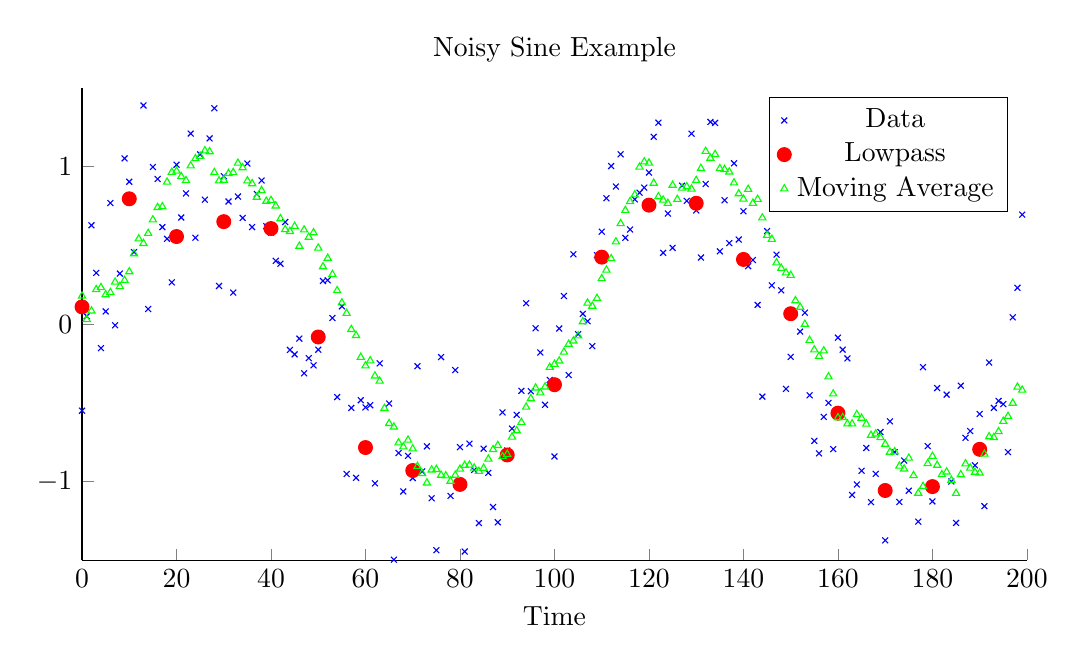
\begin{tikzpicture}
	\begin{axis}[
		scale only axis,
		xmin=0, xmax=200,
		ymin=-1.5, ymax=1.5,
		height=6cm,
		width=12cm,
		title={Noisy Sine Example},
		axis y line*=left,
		axis x line*=bottom,
		xlabel={Time},
%		ylabel style = {align=center},
]
	\addplot[only marks, mark size=1.5pt, color=blue, mark=x] plot coordinates {
(0, -0.5501479053659568)
(1, 0.04990459384452345)
(2, 0.6274596482378976)
(3, 0.3252795490939927)
(4, -0.1525721601066644)
(5, 0.08045921178639026)
(6, 0.7687376729201951)
(7, -0.007442023456780411)
(8, 0.3209010814018999)
(9, 1.05208841474986)
(10, 0.9038952332202342)
(11, 0.45718150346147257)
(12, 1.6664762541804545)
(13, 1.3883841633156073)
(14, 0.0959436126575186)
(15, 0.9973679392272481)
(16, 0.9214109136682133)
(17, 0.6158098747298182)
(18, 0.5416040265267108)
(19, 0.2646717009751939)
(20, 1.011932476020506)
(21, 0.6768968676643023)
(22, 0.8296930066042326)
(23, 1.209785341525421)
(24, 0.5485516614459032)
(25, 1.0777839082776488)
(26, 0.7896732689385482)
(27, 1.1791149144699895)
(28, 1.3704568699815682)
(29, 0.24207850809702192)
(30, 0.9392748489130466)
(31, 0.7785370452836562)
(32, 0.20020296351046263)
(33, 0.8099632853551217)
(34, 0.6743538368037855)
(35, 1.0193955654927778)
(36, 0.6159125285177007)
(37, 0.8261404072490393)
(38, 0.9117925417056809)
(39, 0.6215225947676456)
(40, 0.5809588185644028)
(41, 0.4019145022594688)
(42, 0.38327221035625697)
(43, 0.6480669823667553)
(44, -0.16386652331048945)
(45, -0.19223339327083488)
(46, -0.09212324073050407)
(47, -0.31242926654033143)
(48, -0.21592546607777902)
(49, -0.2622619914035026)
(50, -0.1627244053902957)
(51, 0.27375002459981135)
(52, 0.2784525650397579)
(53, 0.038831383300801436)
(54, -0.46343901515461444)
(55, 0.11272590533163734)
(56, -0.9515291606715435)
(57, -0.5324893121832327)
(58, -0.9762217955659198)
(59, -0.4835228418089682)
(60, -0.5292294456308441)
(61, -0.5152339497449736)
(62, -1.0116413020949682)
(63, -0.2493577870918075)
(64, -1.6908720113839135)
(65, -0.5045375779114657)
(66, -1.4962041524928056)
(67, -0.8187708996173293)
(68, -1.0627533423099704)
(69, -0.8366472774690741)
(70, -0.9774221164797546)
(71, -0.2676469515161257)
(72, -0.9359825987093011)
(73, -0.7761265893265307)
(74, -1.1059930107991471)
(75, -1.4357685797587965)
(76, -0.2096006158605498)
(77, -1.7308359414606433)
(78, -1.090754949582482)
(79, -0.29183268315597066)
(80, -0.7812418179615632)
(81, -1.444216478524424)
(82, -0.7591398796041369)
(83, -0.9262324129533797)
(84, -1.2636676359857844)
(85, -0.7909530875911055)
(86, -0.944653509531513)
(87, -1.161751520485138)
(88, -1.2585194150626422)
(89, -0.5609921300088824)
(90, -0.8025167764777815)
(91, -0.6639830652321672)
(92, -0.5762532433361727)
(93, -0.423857612244092)
(94, 0.1324024568189806)
(95, -0.4261419143534969)
(96, -0.026344729142443846)
(97, -0.18047161328845027)
(98, -0.5122467557921724)
(99, -0.3545616105864788)
(100, -0.8405177798205792)
(101, -0.028144457573901813)
(102, 0.17853701572648664)
(103, -0.32314766411469575)
(104, 0.4430325144960613)
(105, -0.06424053487774661)
(106, 0.065036061140536)
(107, 0.018062195668807957)
(108, -0.13990956902461482)
(109, 0.43775122502468433)
(110, 0.5869578924457315)
(111, 0.7991351296358233)
(112, 1.0034235492594452)
(113, 0.873571937118365)
(114, 1.0780641947371608)
(115, 0.5477616596352353)
(116, 0.6005212099730896)
(117, 0.7917046160964445)
(118, 0.8342073027229107)
(119, 0.8667393789052593)
(120, 0.9623398038328765)
(121, 1.1892238075737607)
(122, 1.27885982958251)
(123, 0.4523791374582725)
(124, 0.702167949665317)
(125, 0.48413090997597763)
(126, 1.5166990521520756)
(127, 0.8788566761195209)
(128, 0.7826252018368195)
(129, 1.2092518246174229)
(130, 0.7218057779949414)
(131, 0.42264264990256695)
(132, 0.8895363765261645)
(133, 1.283874228313099)
(134, 1.27757948471383)
(135, 0.46216923127837584)
(136, 0.7863515877078047)
(137, 0.5139834752396573)
(138, 1.0211820550398865)
(139, 0.5369565276604398)
(140, 0.7164997117186234)
(141, 0.3678037790234276)
(142, 0.40672714527098164)
(143, 0.12220954371571036)
(144, -0.46059409341324475)
(145, 0.5907832762263421)
(146, 0.2457623884873774)
(147, 0.4409423078661675)
(148, 0.21422892756860945)
(149, -0.4112714755373881)
(150, -0.20817634307427632)
(151, 0.7767093551475509)
(152, -0.04757161425795681)
(153, 0.07251523756927367)
(154, -0.45217656415202145)
(155, -0.7418368070125154)
(156, -0.8208541133276354)
(157, -0.5889672570203961)
(158, -0.5002336493132791)
(159, -0.7938121218592649)
(160, -0.0862062100948966)
(161, -0.16220549570511228)
(162, -0.21782160299838704)
(163, -1.0846769445687992)
(164, -1.0183789885190992)
(165, -0.9314119955322128)
(166, -0.7864471463419822)
(167, -1.1307398608616681)
(168, -0.9509763556378509)
(169, -0.6853154902262544)
(170, -1.3733497976734017)
(171, -0.6177713532077902)
(172, -0.8127258791188124)
(173, -1.129310619679885)
(174, -0.866509050453941)
(175, -1.057987736374333)
(176, -1.8041681346555074)
(177, -1.2543172490324743)
(178, -0.2735848851547471)
(179, -0.774793369057666)
(180, -1.1261131824699777)
(181, -0.40632394050647824)
(182, -1.7639931206365895)
(183, -0.4479187722100195)
(184, -0.999762980632152)
(185, -1.2625101996939676)
(186, -0.39125687065756865)
(187, -0.7220483912467909)
(188, -0.6792915449213922)
(189, -0.8971912224923284)
(190, -0.5707331354413933)
(191, -1.1562029062408703)
(192, -0.24394246654784563)
(193, -0.5319624822046162)
(194, -0.4877367782615039)
(195, -0.5079765763210093)
(196, -0.812775012915596)
(197, 0.043029644392428706)
(198, 0.23063472875433633)
(199, 0.6948960783559982)

	};
	\addlegendentry{Data}

\addplot[only marks, mark size=2.5pt, color=red, mark=*] plot coordinates {
(0, 0.10931908740524426)
(10, 0.7955688877386944)
(20, 0.556024964679218)
(30, 0.6506156880761342)
(40, 0.6067859762699795)
(50, -0.08187313255985673)
(60, -0.784050174399075)
(70, -0.9298481832238462)
(80, -1.017984924798253)
(90, -0.83098601245929)
(100, -0.38474284181883467)
(110, 0.4251823409221544)
(120, 0.7553988118000428)
(130, 0.7671737003635911)
(140, 0.41048370621767793)
(150, 0.06597165468760675)
(160, -0.565628462451966)
(170, -1.056603075534645)
(180, -1.0318803873167333)
(190, -0.7951078250252007)
	};
	\addlegendentry{Lowpass}

\addplot[only marks, mark size=1.5pt, color=green, mark=triangle] plot coordinates {
(0, 0.1786166934916299)
(1, 0.029013138330308608)
(2, 0.08361296995604772)
(3, 0.219309713069145)
(4, 0.23220328848172392)
(5, 0.18664476828916574)
(6, 0.2004622278342941)
(7, 0.2671152911230697)
(8, 0.2387934788866389)
(9, 0.2781227085009668)
(10, 0.33270005406312936)
(11, 0.44705344586647716)
(12, 0.5412763969551257)
(13, 0.5124762171096306)
(14, 0.5761068902729938)
(15, 0.6622819366302825)
(16, 0.7407680828533738)
(17, 0.7455217906581544)
(18, 0.9017491296826708)
(19, 0.9641925754813077)
(20, 0.9716167632775722)
(21, 0.9370565556338157)
(22, 0.9117852059744717)
(23, 1.005092617946012)
(24, 1.0510023096328074)
(25, 1.0664873372947525)
(26, 1.1007939366033865)
(27, 1.0950758686227489)
(28, 0.9627808259014834)
(29, 0.9100831135091294)
(30, 0.9140117782524134)
(31, 0.9567140286175275)
(32, 0.9626303951151964)
(33, 1.0222100233856573)
(34, 0.9929999434698444)
(35, 0.909735245035527)
(36, 0.8919431890288448)
(37, 0.8058656350927486)
(38, 0.849023926100265)
(39, 0.780409700475769)
(40, 0.7857047927490054)
(41, 0.7507188919459147)
(42, 0.6695640504639723)
(43, 0.6007535446422407)
(44, 0.5883137882481028)
(45, 0.621289549938386)
(46, 0.49465054247642976)
(47, 0.5983635625728109)
(48, 0.5520664028155926)
(49, 0.5804601228659143)
(50, 0.4830779851015157)
(51, 0.36456948485296303)
(52, 0.41847335074282765)
(53, 0.3153345812478249)
(54, 0.21316551297172287)
(55, 0.13501405116239334)
(56, 0.0685873113637486)
(57, -0.03373079835409383)
(58, -0.07200638756667536)
(59, -0.21070077094565)
(60, -0.26490819714981423)
(61, -0.2326577151301032)
(62, -0.32923245116457456)
(63, -0.3620980744856616)
(64, -0.5353244850405338)
(65, -0.6309338551785377)
(66, -0.6532899425694172)
(67, -0.7540207550784115)
(68, -0.7793589941138287)
(69, -0.7364814224888521)
(70, -0.7919858358908411)
(71, -0.9035227152862925)
(72, -0.9482176419524888)
(73, -1.0083091278343994)
(74, -0.9258642957290864)
(75, -0.9225922500738062)
(76, -0.9591551186017018)
(77, -0.9631722851859379)
(78, -0.9974053878259838)
(79, -0.9595825656036256)
(80, -0.9208082427003987)
(81, -0.8964342644894547)
(82, -0.8947605077752024)
(83, -0.9136833195679064)
(84, -0.9349195158634582)
(85, -0.9148524999818365)
(86, -0.856822145980406)
(87, -0.7966264563450041)
(88, -0.7703145991647626)
(89, -0.8414759157841492)
(90, -0.8267796155927432)
(91, -0.7169078002199846)
(92, -0.676693039548897)
(93, -0.6237425110754458)
(94, -0.5268180584662999)
(95, -0.4733108392429567)
(96, -0.4056073626921776)
(97, -0.4365555248303029)
(98, -0.39899945229505684)
(99, -0.2743604051000976)
(100, -0.25509777765705344)
(101, -0.23363278665860712)
(102, -0.17759390441393544)
(103, -0.12776008144874113)
(104, -0.10702371353088977)
(105, -0.07389920813448543)
(106, 0.015319788266465118)
(107, 0.13356340995069096)
(108, 0.11401885556967686)
(109, 0.16340118833963668)
(110, 0.28895396737521606)
(111, 0.34355149566501647)
(112, 0.4158770605332518)
(113, 0.5224288852441129)
(114, 0.6382959346306375)
(115, 0.722179761647036)
(116, 0.7786131422260906)
(117, 0.8212698513643033)
(118, 0.9972651690826899)
(119, 1.030638474444876)
(120, 1.0229367282211461)
(121, 0.8949750539704129)
(122, 0.8088859886246633)
(123, 0.7876830800437209)
(124, 0.7666872423455546)
(125, 0.8819100181735479)
(126, 0.7922002061455957)
(127, 0.8641173786239922)
(128, 0.872768357073604)
(129, 0.8578630535630369)
(130, 0.912037109565478)
(131, 0.9886390391465245)
(132, 1.0969538115282258)
(133, 1.053703176000814)
(134, 1.07764401364253)
(135, 0.987724555508984)
(136, 0.982294078118095)
(137, 0.9663275376951097)
(138, 0.8970575631064467)
(139, 0.8279541881660226)
(140, 0.7939582379429274)
(141, 0.8559953465595344)
(142, 0.7674897238180931)
(143, 0.792540651289289)
(144, 0.6747901216303511)
(145, 0.5639203400012163)
(146, 0.5388754252363867)
(147, 0.38966116394196215)
(148, 0.3543616378617186)
(149, 0.325746577083447)
(150, 0.3101708449476802)
(151, 0.14887989391145323)
(152, 0.10721971617833237)
(153, -0.0007195140619984386)
(154, -0.1027984275281065)
(155, -0.16312725072940795)
(156, -0.20447895358142176)
(157, -0.16938239981223027)
(158, -0.33459175384422457)
(159, -0.44305864631881775)
(160, -0.5940318094938636)
(161, -0.5929346719916628)
(162, -0.6335799782459096)
(163, -0.6330037360694498)
(164, -0.574030204252528)
(165, -0.5974213113560747)
(166, -0.6346020125059428)
(167, -0.7058348795165471)
(168, -0.6973240363678268)
(169, -0.7207788567850656)
(170, -0.7625762930891603)
(171, -0.8131456844407591)
(172, -0.8100062892419961)
(173, -0.9015903301456822)
(174, -0.9197637253516298)
(175, -0.8506585942768558)
(176, -0.9614700810648353)
(177, -1.073769505787915)
(178, -1.0306980718030587)
(179, -0.8854291090126987)
(180, -0.8390938807530338)
(181, -0.8960521359463229)
(182, -0.9555796723514778)
(183, -0.9388154565148306)
(184, -0.9909236169929627)
(185, -1.0748452537850757)
(186, -0.9560036528298396)
(187, -0.8870411921971437)
(188, -0.9138548706509179)
(189, -0.9405948158661428)
(190, -0.9453532207257522)
(191, -0.8256677055985545)
(192, -0.7149483230221129)
(193, -0.7199574273058152)
(194, -0.6824419941967865)
(195, -0.6171069752778036)
(196, -0.5859382346398394)
(197, -0.5019335628985753)
(198, -0.40016461029164746)
(199, -0.4192276636482304)
};
\addlegendentry{Moving Average}
	\end{axis}
\end{tikzpicture}

	\caption{Example of smoothing a noisy sine signal measured with a high sample rate.}
	\label{f:noise_example}
	\end{figure}
	
	\subsection{Anomalous Values}
	Anomaly Detection is technically a whole chapter on its own. Here we care only about the values that are obviously anomalous as the might be out of their possible range or not even a number. Even though one point in a thousand might not seem severe and will most likely not disturb the models performance much, they are an easy catch and can still help improve the analysis.
	
	In our case no severe anomalous points were discovered except for the gaps mentioned in the section before.
	
	\subsection{Normalizing}
	Normalizing values is especially important when dealing with \acp{nn} \cite[p. 101ff]{python-deep-learning}. One reason is to avoid having small values that might be subject to rounding errors. The same holds true for big values or negative values that might not be representable.	There are two general approaches to normalization. 
	
	First and most common one is subtracting the mean and dividing by the standard-deviation: 

	\begin{equation}
	\tilde{\mathbf{x}} = \frac{\mathbf{x} - \overline{\mathbf{x}}}{\sigma}
	\end{equation}		
	
	The second one works by moving all values to a range of $\tilde{\mathbf{x}}\in [0, 1]$ by finding the minimum and maximum of the dataset: 
	
	\begin{equation}
	\tilde{\mathbf{x}} = \frac{\mathbf{x} - \min \{\mathbf{x}\}}{\max\{\mathbf{x}\} - \min\{\mathbf{x}\}}
	\end{equation}		

	In this thesis we decided for the latter as this technique is easily applicable on spacecraft as we are already doing boundary checks with fixed minimum and maximum values.
	
	For \ac{ml} applications there is one thing to consider: \underline{which} part of the data provides the normalization. As the datasets are usually divided into training, validation and test-set, only the training-set is used to calculate the minimum, maximum, mean and variance, to not leak any information of the test data into the learning process.

	\subsection{Feature Engineering}
	Feature Engineering takes a huge part in the success and failure of \ac{ml} models. Here we need to select the right features/parameters, transform them or even generate artificial ones.
	
	For selecting the correct features, there are no general rules or recipes, they just have to be guessed and tried by the engineer. But in the following is a guide on how to understand, sort and work with different parameters.
	
		\subsubsection{Deterministic Parameter}
		As the name suggests, deterministic parameters are known at any given timepoint $t$. These are for example all parameters that are set or configured in the spacecraft, like an engine or subsystem switching on and off, or the positioning of the solar array. \newline
		Some parameters can also be put in this category, if they are easy to extrapolate, like the orbit or position in the solar system.
		
		For the \ac{rwa} of Rosetta, the deterministic parameters were the speed of the wheels and direction. And for the solar array only the position of the array w.r.t. to the spacecraft itself.
		
		\subsubsection{Aleatoric Parameter}
		Aleatoric parameters are the opposite of deterministic features, they are only known from past measurements and cannot be extrapolated into the feature easily. This concerns temperatures, voltages, currents, rf-signals and any scientific measurement.
		
		\subsubsection{One-Hot Encoding}
		One-Hot encoding is an important feature when using \ac{ml}. Here the state of a parameter can be described with discrete states instead of continues values. This transformation works with any kind of parameter that has discrete states. An example flow is shown in the following:

		\begin{equation*}
		\mathbf{x} = \begin{pmatrix}
		\text{Monday} \\
		\text{Wednesday} \\
		\text{Friday} \\
		\text{Monday} \\
		\text{Thursday} \\
		\text{Saturday} \\
		\end{pmatrix} \rightarrow
		\mathbf{x} = \begin{bmatrix}
		1 & 0 & 0 & 0 & 0 & 0 & 0 \\
		0 & 0 & 1 & 0 & 0 & 0 & 0 \\
		0 & 0 & 0 & 0 & 1 & 0 & 0 \\
		1 & 0 & 0 & 0 & 0 & 0 & 0 \\
		0 & 0 & 0 & 1 & 0 & 0 & 0 \\
		0 & 0 & 0 & 0 & 0 & 1 & 0 \\
		\end{bmatrix}
		\end{equation*}				
		
		With the example of the \ac{rwa} of Rosetta, the parameter for the wheel direction was saved as a plain number. Zero for backward, one for forward. This value was transformed to a discrete integer and not subject to the normalization, so it could be used in a one-hot encoding matrix.		
		
		\subsubsection{Artificial Features}
		One can also create features to support the learning process. A starting point for that are periodic processes like a satellite orbiting earth. The orbit itself might not appear in the measured parameters directly, but it can be superimposed as the orbit parameters are known. A sine and cosine with the orbit periodicity can be added to aid the learning process. Additionally a second sine and cosine can be applied with the periodicity of the earth moving around sun to further support seasonal changes. Figure \ref{f:artificial_feature_example} shows an example flow-chart for artificial features to keep in mind for future engineering tasks.
		
		Artificial features can be of course included in the deterministic features.
		
		\begin{figure}[htb]
		\centering
		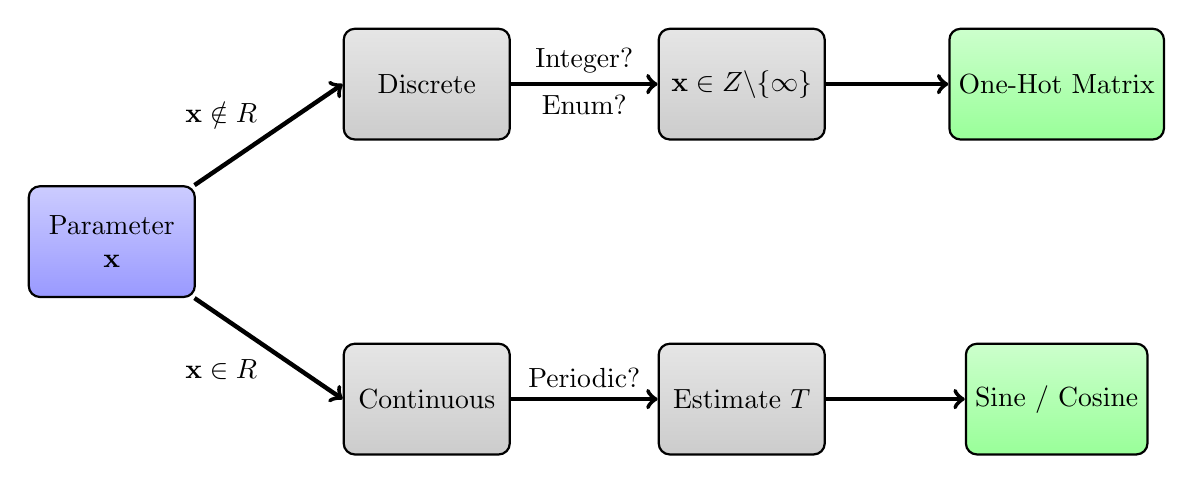
\begin{tikzpicture}[
	input/.style={
		rectangle,
		draw=black,
		thick,
		align=center,
		rounded corners,
		top color=blue!20,
		bottom color=blue!40,
		minimum height=4em,
		minimum width=6em
	},
	trafo/.style={
		rectangle,
		draw=black,
		thick,
		align=center,
		rounded corners,
		top color=gray!20,
		bottom color=gray!40,
		minimum height=4em,
		minimum width=6em
	},
	output/.style={
		rectangle,
		draw=black,
		thick,
		align=center,
		rounded corners,
		top color=green!20,
		bottom color=green!40,
		minimum height=4em,
		minimum width=6em
	},
]

\node[input] (parameter) at (-6, 0) {Parameter \\ $\mathbf{x}$};

\node[trafo] (dis) at (-2, 2) {Discrete};
\node[trafo] (int) at (2, 2) {$\mathbf{x} \in \mathbb{Z} \backslash \{\infty\}$};

\draw[ultra thick,->] (parameter) -- node [above left] {$\mathbf{x} \notin \mathbb{R}$} (dis.west);
\draw[ultra thick,->] (dis) -- node [above] {Integer?} node [below] {Enum?}  (int);

\node[output] (one) at (6, 2) {One-Hot Matrix};

\draw[ultra thick,->] (int) -- (one);

\node[trafo] (con) at (-2, -2) {Continuous};
\node[trafo] (per) at (2, -2) {Estimate $T$};

\draw[ultra thick,->] (parameter) -- node [below left] {$\mathbf{x} \in \mathbb{R}$} (con.west);
\draw[ultra thick,->] (con) -- node [above] {Periodic?} (per);

\node[output] (sin) at (6, -2) {Sine / Cosine};

\draw[ultra thick,->] (per) -- (sin);

\end{tikzpicture}

		\caption{Quick flow-chart to generate artificial features}
		\label{f:artificial_feature_example}
		\end{figure}
		
\section{Fourier Transformation}
The Fourier Transformation brings the time signal into a frequency domain. Here its used to get an overview of the frequencies present in our time-series. Sometimes a seasonal trend or anomalous oscillation can be identified. For later steps it might also be useful in case we need to choose an appropriate windowing size.

For our data, the time window for the \ac{ft} was chosen to be in the length of $T = \SI{90}{day}$ (approximately one quarter year) with the above mentioned samplerate of $t_s = \SI{60}{\minute}$. The windows were set to be 50\% overlapping when sliding over the series. No specific windowing function was applied, which results in a rectangular window. In the end, the windowed \ac{ft} results were summed up to show the spectrum of the whole series.

For all data (\ac{rwa} and solar array), no special peaks could be found. All plots did show high values in the lower frequencies and were monotonically decreasing with the exception of noise over the whole spectrum. In figure \ref{f:rwl_fft} the spectrum of the friction coefficient parameter of all four reaction wheels can be seen. For most part, all four wheels follow the same curve. Slight exceptions are only within wheel B and C at the beginning and end of the spectrum. This might already indicate an anomaly or just be a coincidence.

\begin{figure}[htb]
\centering
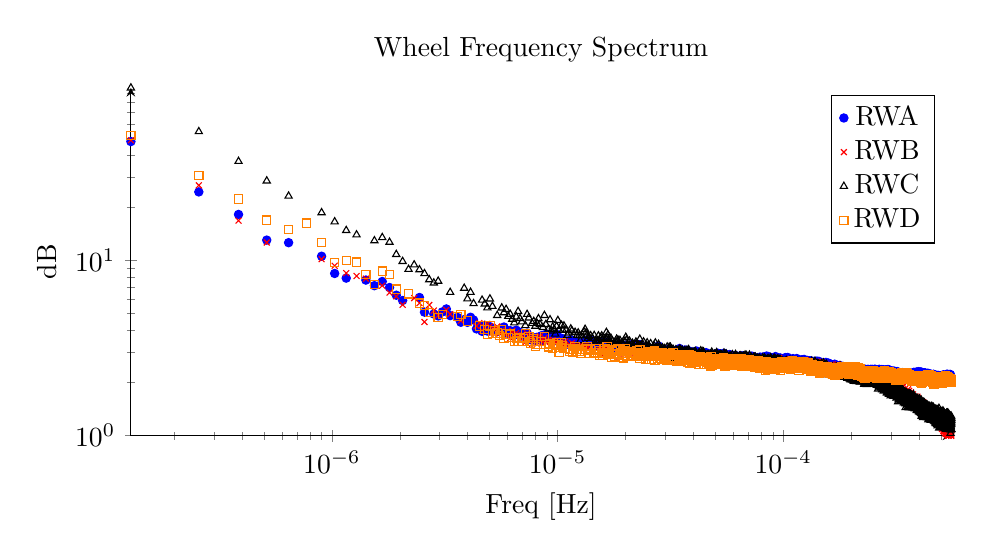
\begin{tikzpicture}
	\begin{loglogaxis}[
		height=6cm,
		width=12cm,
		log basis y=10,
		log basis x=10,
		xlabel={Freq [Hz]},
		ylabel={dB},
		title={Wheel Frequency Spectrum},
		axis x line=bottom,
		axis y line=left,
]
	\addplot[only marks, mark size=1.5pt, color=blue, mark=*] plot coordinates {
		(0.0, 117.831338321829)
		(1.28600823045268e-07, 47.7824333240092)
		(2.57201646090535e-07, 24.6237518787363)
		(3.85802469135802e-07, 18.298244387718)
		(5.1440329218107e-07, 13.0554081935431)
		(6.43004115226338e-07, 12.6205605311199)
		(9.00205761316873e-07, 10.5552996252439)
		(1.02880658436214e-06, 8.41259322243796)
		(1.15740740740741e-06, 7.91541685684246)
		(1.41460905349794e-06, 7.71306021806831)
		(1.54320987654321e-06, 7.16406904691753)
		(1.67181069958848e-06, 7.56801563795429)
		(1.80041152263375e-06, 6.9915793537857)
		(1.92901234567901e-06, 6.31916062570811)
		(2.05761316872428e-06, 5.89253045058042)
		(2.44341563786008e-06, 6.13150649488383)
		(2.57201646090535e-06, 5.05625066857311)
		(2.82921810699589e-06, 4.93618253006117)
		(2.95781893004115e-06, 4.81078808491354)
		(3.08641975308642e-06, 5.07043093871939)
		(3.21502057613169e-06, 5.27242135535563)
		(3.34362139917696e-06, 4.83116637764509)
		(3.60082304526749e-06, 4.71904526851241)
		(3.72942386831276e-06, 4.42579497032112)
		(3.85802469135802e-06, 4.58122041244982)
		(3.98662551440329e-06, 4.42201259811911)
		(4.11522633744856e-06, 4.72602573715385)
		(4.24382716049383e-06, 4.55889096039155)
		(4.3724279835391e-06, 4.05677562793084)
		(4.50102880658436e-06, 4.201665456929)
		(4.62962962962963e-06, 3.92785032538931)
		(4.7582304526749e-06, 4.24395696854642)
		(4.88683127572017e-06, 3.94273977545108)
		(5.01543209876543e-06, 4.17501315374293)
		(5.40123456790124e-06, 3.91706440638256)
		(5.5298353909465e-06, 4.0029964775936)
		(5.78703703703704e-06, 4.15679938266317)
		(5.91563786008231e-06, 3.99407053493608)
		(6.04423868312757e-06, 3.82799201582356)
		(6.17283950617284e-06, 3.96350417384202)
		(6.30144032921811e-06, 3.78369444238308)
		(6.43004115226338e-06, 3.89687233890368)
		(6.55864197530864e-06, 3.986581873962)
		(6.68724279835391e-06, 3.74133480223145)
		(6.81584362139918e-06, 3.87431986239)
		(6.94444444444445e-06, 3.69778588407918)
		(7.33024691358025e-06, 3.83888429170429)
		(7.58744855967078e-06, 3.5257545417963)
		(7.71604938271605e-06, 3.63875071241257)
		(7.97325102880659e-06, 3.48843207929714)
		(8.10185185185185e-06, 3.62828435890682)
		(8.48765432098766e-06, 3.70799399472068)
		(8.61625514403292e-06, 3.4925441791526)
		(8.74485596707819e-06, 3.7493418148462)
		(8.87345679012346e-06, 3.5988762601422)
		(9.00205761316873e-06, 3.76784457905084)
		(9.13065843621399e-06, 3.66009682710673)
		(9.25925925925926e-06, 3.75575033845836)
		(9.38786008230453e-06, 3.54758667179328)
		(9.5164609053498e-06, 3.61905116681968)
		(9.64506172839506e-06, 3.51794768427034)
		(9.9022633744856e-06, 3.78030289903148)
		(1.00308641975309e-05, 3.67017001447895)
		(1.01594650205761e-05, 3.41545252323823)
		(1.05452674897119e-05, 3.56320326199526)
		(1.09310699588477e-05, 3.4342554466337)
		(1.11882716049383e-05, 3.30906545799082)
		(1.14454732510288e-05, 3.51795914793415)
		(1.17026748971193e-05, 3.34411655407217)
		(1.18312757201646e-05, 3.43802240727525)
		(1.19598765432099e-05, 3.30803498475549)
		(1.23456790123457e-05, 3.37563571488337)
		(1.26028806584362e-05, 3.28775893867088)
		(1.28600823045268e-05, 3.3894957435626)
		(1.33744855967078e-05, 3.48986363689749)
		(1.35030864197531e-05, 3.40302719795396)
		(1.36316872427984e-05, 3.26364790975563)
		(1.38888888888889e-05, 3.38843794458689)
		(1.40174897119342e-05, 3.51771733194485)
		(1.41460905349794e-05, 3.40947976548493)
		(1.42746913580247e-05, 3.27801199170795)
		(1.4917695473251e-05, 3.37185586673282)
		(1.53034979423868e-05, 3.20125421886145)
		(1.55606995884774e-05, 3.31872204571544)
		(1.56893004115226e-05, 3.41342148625292)
		(1.58179012345679e-05, 3.23705349110355)
		(1.60751028806584e-05, 3.35864900215495)
		(1.62037037037037e-05, 3.25584434633021)
		(1.6332304526749e-05, 3.32295140154841)
		(1.64609053497942e-05, 3.39130250677572)
		(1.65895061728395e-05, 3.25637861964569)
		(1.67181069958848e-05, 3.409307251421)
		(1.684670781893e-05, 3.23017941182341)
		(1.76183127572016e-05, 3.13051954491365)
		(1.77469135802469e-05, 3.20317766574753)
		(1.78755144032922e-05, 3.28323177499468)
		(1.81327160493827e-05, 3.16904141986705)
		(1.8261316872428e-05, 3.2384218645333)
		(1.87757201646091e-05, 3.06762733280211)
		(1.89043209876543e-05, 3.20482991104786)
		(1.90329218106996e-05, 3.28693890202065)
		(1.91615226337449e-05, 3.15285031748545)
		(1.92901234567901e-05, 3.07994394883357)
		(1.94187242798354e-05, 3.25791608150576)
		(1.98045267489712e-05, 3.19022437720887)
		(1.99331275720165e-05, 3.26605630058796)
		(2.0190329218107e-05, 3.18205295599571)
		(2.07047325102881e-05, 3.10544616523812)
		(2.08333333333333e-05, 3.17929466163994)
		(2.12191358024691e-05, 3.08428136728029)
		(2.13477366255144e-05, 3.24542126773882)
		(2.14763374485597e-05, 3.31113987680514)
		(2.16049382716049e-05, 3.24434550103776)
		(2.18621399176955e-05, 3.12519443652999)
		(2.31481481481481e-05, 3.30117616289776)
		(2.32767489711934e-05, 3.23471208485988)
		(2.36625514403292e-05, 3.11429058251684)
		(2.49485596707819e-05, 3.20687761880889)
		(2.52057613168724e-05, 3.01399830108765)
		(2.53343621399177e-05, 3.07613024162769)
		(2.62345679012346e-05, 3.01125712901042)
		(2.63631687242798e-05, 3.11082364944196)
		(2.68775720164609e-05, 2.98049487909967)
		(2.71347736625514e-05, 3.05740871237194)
		(2.7906378600823e-05, 3.13603291976797)
		(2.80349794238683e-05, 3.23688047962303)
		(2.84207818930041e-05, 3.11404213706997)
		(2.86779835390946e-05, 3.04545022717448)
		(2.91923868312757e-05, 2.94113642457141)
		(2.94495884773663e-05, 3.05971078087673)
		(3.02211934156379e-05, 2.99229527961171)
		(3.06069958847737e-05, 3.07664767991279)
		(3.07355967078189e-05, 3.01066281485919)
		(3.11213991769547e-05, 3.10239681313513)
		(3.17644032921811e-05, 3.0003009941548)
		(3.39506172839506e-05, 3.07637948075171)
		(3.40792181069959e-05, 3.0130790767079)
		(3.47222222222222e-05, 3.13211422630134)
		(3.48508230452675e-05, 3.03569479081063)
		(3.53652263374486e-05, 2.90402263445777)
		(3.56224279835391e-05, 3.01615473557031)
		(3.58796296296296e-05, 2.93807725881814)
		(3.63940329218107e-05, 2.86601968076423)
		(3.6522633744856e-05, 2.9972944545102)
		(3.66512345679012e-05, 3.06538742201482)
		(3.67798353909465e-05, 2.97587612611577)
		(3.69084362139918e-05, 3.05591813581287)
		(3.7037037037037e-05, 2.98882804452284)
		(3.74228395061728e-05, 3.0582953360631)
		(3.79372427983539e-05, 2.97090224884659)
		(3.80658436213992e-05, 3.04106896335293)
		(3.87088477366255e-05, 2.96590858298978)
		(3.94804526748971e-05, 2.87357836751478)
		(3.96090534979424e-05, 2.9371129038127)
		(4.0380658436214e-05, 3.00155127596333)
		(4.10236625514403e-05, 2.9384273332606)
		(4.12808641975309e-05, 3.03109229439007)
		(4.16666666666667e-05, 2.93320691642606)
		(4.35956790123457e-05, 2.85385316842459)
		(4.43672839506173e-05, 2.93248000822877)
		(4.53960905349794e-05, 2.86404904791863)
		(4.55246913580247e-05, 2.96611044826892)
		(4.565329218107e-05, 2.90477170818297)
		(4.69393004115226e-05, 2.84598338071461)
		(4.73251028806584e-05, 2.91189024039263)
		(4.86111111111111e-05, 2.82788850277208)
		(4.91255144032922e-05, 2.88917805618524)
		(4.96399176954732e-05, 2.80991187572331)
		(4.98971193415638e-05, 2.90530801682567)
		(5.00257201646091e-05, 2.8462538620872)
		(5.11831275720165e-05, 2.94468597402322)
		(5.15689300411523e-05, 2.85755748828163)
		(5.24691358024691e-05, 2.92147794977886)
		(5.25977366255144e-05, 2.81003640211495)
		(5.29835390946502e-05, 2.89402693164437)
		(5.3369341563786e-05, 2.83010413083899)
		(5.34979423868313e-05, 2.75616913591156)
		(5.37551440329218e-05, 2.84859164283658)
		(5.45267489711934e-05, 2.94294146701497)
		(5.49125514403292e-05, 2.87856705347238)
		(5.50411522633745e-05, 2.81048030410384)
		(5.54269547325103e-05, 2.89216536077726)
		(5.56841563786008e-05, 2.83251730487077)
		(5.58127572016461e-05, 2.89053636756872)
		(5.65843621399177e-05, 2.8177285431322)
		(5.78703703703704e-05, 2.89420949578174)
		(5.81275720164609e-05, 2.83413132066339)
		(5.82561728395062e-05, 2.77359980798008)
		(5.9156378600823e-05, 2.83754048046293)
		(5.96707818930041e-05, 2.75057923240172)
		(5.97993827160494e-05, 2.85053826286994)
		(6.01851851851852e-05, 2.74931862217311)
		(6.03137860082305e-05, 2.82808824576449)
		(6.21141975308642e-05, 2.76641661111111)
		(6.22427983539095e-05, 2.84110014560116)
		(6.30144032921811e-05, 2.7766144684912)
		(6.48148148148148e-05, 2.84434349904384)
		(6.49434156378601e-05, 2.77452125251309)
		(6.6358024691358e-05, 2.8453073848796)
		(6.66152263374486e-05, 2.73582216807189)
		(6.70010288065844e-05, 2.80188941465188)
		(6.76440329218107e-05, 2.74454342852874)
		(6.7772633744856e-05, 2.82129254894147)
		(6.8287037037037e-05, 2.76055902573419)
		(6.88014403292181e-05, 2.81830314649697)
		(7.07304526748971e-05, 2.75473160955169)
		(7.09876543209877e-05, 2.8131530444704)
		(7.15020576131687e-05, 2.74065527315357)
		(7.25308641975309e-05, 2.83413710551042)
		(7.30452674897119e-05, 2.73143572017336)
		(7.3559670781893e-05, 2.81556425085474)
		(7.39454732510288e-05, 2.73189873153997)
		(7.42026748971193e-05, 2.79655748847928)
		(7.62602880658436e-05, 2.73358685862706)
		(7.89609053497942e-05, 2.79812615190498)
		(7.92181069958848e-05, 2.73449146392479)
		(8.1275720164609e-05, 2.79750245899817)
		(8.14043209876543e-05, 2.72515494038637)
		(8.21759259259259e-05, 2.79665072551323)
		(8.29475308641975e-05, 2.73621744279044)
		(8.34619341563786e-05, 2.79630939882888)
		(8.38477366255144e-05, 2.73518290974199)
		(8.43621399176955e-05, 2.83701617625193)
		(8.4619341563786e-05, 2.71220794436979)
		(8.50051440329218e-05, 2.7744874725077)
		(8.55195473251029e-05, 2.70952244587066)
		(8.57767489711934e-05, 2.81593158627663)
		(8.62911522633745e-05, 2.7430346870044)
		(8.64197530864198e-05, 2.65385747166268)
		(8.66769547325103e-05, 2.71480047737546)
		(8.69341563786008e-05, 2.78003749276777)
		(8.73199588477366e-05, 2.71702682359082)
		(8.77057613168724e-05, 2.78639189317884)
		(8.95061728395062e-05, 2.70587366272146)
		(9.05349794238683e-05, 2.76084971306653)
		(9.10493827160494e-05, 2.67271465930554)
		(9.14351851851852e-05, 2.76710406044573)
		(9.16923868312757e-05, 2.67176175189267)
		(9.22067901234568e-05, 2.74716840312927)
		(9.24639917695473e-05, 2.81718218816513)
		(9.25925925925926e-05, 2.73824394901247)
		(9.28497942386831e-05, 2.66159396608219)
		(9.36213991769547e-05, 2.74042138681317)
		(9.40072016460905e-05, 2.68154602364329)
		(9.42644032921811e-05, 2.76638249406098)
		(9.45216049382716e-05, 2.70867424176918)
		(9.68364197530864e-05, 2.76862346609849)
		(9.72222222222222e-05, 2.67039905007993)
		(9.73508230452675e-05, 2.73594423478065)
		(9.94084362139918e-05, 2.660673580151)
		(9.9537037037037e-05, 2.71900643208234)
		(0.000102237654321, 2.77832288480206)
		(0.00010262345679, 2.64991318038178)
		(0.000102880658436, 2.73524546450356)
		(0.000103652263374, 2.67149325823589)
		(0.000103909465021, 2.768778879477)
		(0.000104166666667, 2.68926872261154)
		(0.000104809670782, 2.78337613978893)
		(0.000104938271605, 2.71086022930793)
		(0.000109053497942, 2.62927388529724)
		(0.000109182098765, 2.68600953161767)
		(0.000110468106996, 2.74190419931489)
		(0.000110596707819, 2.67785410668007)
		(0.000114711934156, 2.74524979570763)
		(0.000114969135802, 2.6612495879675)
		(0.000115612139918, 2.72023654514305)
		(0.000115869341564, 2.65842249462724)
		(0.000118312757202, 2.60493243076866)
		(0.000118441358025, 2.67477892841788)
		(0.000119855967078, 2.61823662292945)
		(0.000120113168724, 2.69441601557362)
		(0.000121527777778, 2.62826867293774)
		(0.000121656378601, 2.6946762995997)
		(0.000122299382716, 2.63656482937563)
		(0.000122813786008, 2.69048254541164)
		(0.000122942386831, 2.62350609548952)
		(0.00012371399177, 2.71267391918505)
		(0.000124099794239, 2.6158602345819)
		(0.000124871399177, 2.67603566322046)
		(0.000127572016461, 2.62245437654001)
		(0.000128086419753, 2.67502678400615)
		(0.000128472222222, 2.609008969252)
		(0.000130272633745, 2.66337249862613)
		(0.000132458847737, 2.58832728734889)
		(0.000132716049383, 2.66491491216972)
		(0.000132973251029, 2.60785482929617)
		(0.000135673868313, 2.55555148322436)
		(0.000135802469136, 2.637277129661)
		(0.000136574074074, 2.55993130561988)
		(0.00013683127572, 2.63576434871106)
		(0.000137088477366, 2.58087579179333)
		(0.000137602880658, 2.63740726924084)
		(0.000138760288066, 2.57859627475881)
		(0.000139274691358, 2.64730512747287)
		(0.000139660493827, 2.59020473577175)
		(0.000141203703704, 2.65092186344176)
		(0.00014146090535, 2.57400438559476)
		(0.000143904320988, 2.64425452209264)
		(0.00014441872428, 2.5818365812501)
		(0.000148148148148, 2.52420497922789)
		(0.000148276748971, 2.59376532793835)
		(0.000150848765432, 2.51195159366738)
		(0.000151234567901, 2.58492302488326)
		(0.00015162037037, 2.51445041776382)
		(0.000151877572016, 2.56789387921607)
		(0.000152649176955, 2.49584986521838)
		(0.000152906378601, 2.55407610446134)
		(0.000154320987654, 2.49686837174178)
		(0.000154449588477, 2.55131399736776)
		(0.000154706790123, 2.6073230823533)
		(0.00015496399177, 2.5331006732021)
		(0.000158436213992, 2.58694837633095)
		(0.000158822016461, 2.48723480370901)
		(0.000159336419753, 2.54947986601104)
		(0.000159850823045, 2.4732660585224)
		(0.000160236625514, 2.53439756303751)
		(0.000160622427984, 2.48145272592119)
		(0.000161008230453, 2.55684650735902)
		(0.000161394032922, 2.49283712113269)
		(0.000161779835391, 2.54480688304459)
		(0.000162294238683, 2.4774897655326)
		(0.000162680041152, 2.5365517730525)
		(0.000165252057613, 2.45922032491532)
		(0.000165637860082, 2.51076293999277)
		(0.00016808127572, 2.4489301467604)
		(0.000168338477366, 2.53773652717172)
		(0.000168852880658, 2.4593414717908)
		(0.000169238683128, 2.5455666231096)
		(0.000169367283951, 2.48728020014033)
		(0.000170010288066, 2.42981234693902)
		(0.000170267489712, 2.52750404882578)
		(0.000170524691358, 2.44667526123383)
		(0.000178240740741, 2.50541726128124)
		(0.00017862654321, 2.42479560616643)
		(0.000179783950617, 2.47485640517794)
		(0.000180298353909, 2.41342655004293)
		(0.000181455761317, 2.47317702404743)
		(0.000181970164609, 2.4176414473337)
		(0.000186085390947, 2.36608056648837)
		(0.000186342592593, 2.45008865694146)
		(0.000186728395062, 2.37764498484462)
		(0.000190715020576, 2.45692696389667)
		(0.000190972222222, 2.37338114101002)
		(0.000191358024691, 2.42964619654639)
		(0.000191872427984, 2.34749440642602)
		(0.000192258230453, 2.42401526487685)
		(0.000192515432099, 2.36582557049461)
		(0.000192901234568, 2.41769061525326)
		(0.00019341563786, 2.36622572610601)
		(0.000196116255144, 2.41852895804423)
		(0.000196502057613, 2.36769365371589)
		(0.000198302469136, 2.31750244087629)
		(0.000198431069959, 2.37561658054567)
		(0.000199974279835, 2.32049648886514)
		(0.000200360082305, 2.37246868369828)
		(0.000203060699588, 2.32401117983661)
		(0.000204346707819, 2.38551957372775)
		(0.000204603909465, 2.3305187437554)
		(0.00020691872428, 2.39207047343546)
		(0.000208076131687, 2.34365009673102)
		(0.000208976337449, 2.29422453942682)
		(0.000209362139918, 2.38312228156195)
		(0.000209747942387, 2.32389005005777)
		(0.000211033950617, 2.37521725076662)
		(0.000211419753086, 2.29651394431411)
		(0.000212191358025, 2.34882842187175)
		(0.000212448559671, 2.29920684063211)
		(0.00021283436214, 2.38901364555849)
		(0.000213091563786, 2.32989366146474)
		(0.000214248971193, 2.37727948478226)
		(0.000215020576132, 2.32228565618885)
		(0.000217721193416, 2.3782823520773)
		(0.000217849794239, 2.32422472294905)
		(0.000219778806584, 2.27145426000661)
		(0.000219907407407, 2.32110168592776)
		(0.000220936213992, 2.37320101621619)
		(0.000221064814815, 2.32295826533917)
		(0.000222093621399, 2.26952962485146)
		(0.000222479423868, 2.32239291282628)
		(0.000226208847737, 2.27348127056619)
		(0.000226466049383, 2.35087314055)
		(0.000226980452675, 2.29149895163922)
		(0.000227237654321, 2.35157263248676)
		(0.000227366255144, 2.4014457048581)
		(0.00022762345679, 2.31301196028021)
		(0.000228395061728, 2.37388640892315)
		(0.000228523662551, 2.29901375666883)
		(0.000228909465021, 2.34514663072792)
		(0.000229423868313, 2.29223933813099)
		(0.000229938271605, 2.34374991010644)
		(0.000230324074074, 2.29518870748845)
		(0.00023058127572, 2.34112235403752)
		(0.000231224279835, 2.2829094151086)
		(0.000231738683128, 2.34951625128685)
		(0.00023521090535, 2.28166067427653)
		(0.000235468106996, 2.33013272709888)
		(0.000235982510288, 2.28167504645233)
		(0.000236368312757, 2.36447449516059)
		(0.000236882716049, 2.28742031767669)
		(0.000237268518519, 2.38065878303414)
		(0.000237654320988, 2.31274734360568)
		(0.00023816872428, 2.36568478638099)
		(0.000238425925926, 2.31298663275418)
		(0.000239197530864, 2.36445160128193)
		(0.000239326131687, 2.29182291993286)
		(0.000239711934156, 2.34399657962748)
		(0.000240354938272, 2.29008712088822)
		(0.000240483539095, 2.33775293773462)
		(0.00024112654321, 2.28287027484944)
		(0.000241769547325, 2.3323952675802)
		(0.000243569958848, 2.2764787887192)
		(0.000243698559671, 2.32552949961969)
		(0.000244470164609, 2.38000200608114)
		(0.000244855967078, 2.30732285771228)
		(0.00024537037037, 2.37030366777907)
		(0.000245498971193, 2.30749848093741)
		(0.000246270576132, 2.35367359404352)
		(0.000246656378601, 2.29507180143008)
		(0.000247170781893, 2.36753502214679)
		(0.000247427983539, 2.29148593551567)
		(0.000248199588477, 2.36990458070607)
		(0.0002483281893, 2.30721216245683)
		(0.000248842592593, 2.37750784616171)
		(0.000248971193416, 2.32934844352499)
		(0.000253729423868, 2.37750425603024)
		(0.000253986625514, 2.32060835208355)
		(0.000255272633745, 2.38429965775475)
		(0.000255529835391, 2.31605041667927)
		(0.000264917695473, 2.37570612179319)
		(0.000265303497942, 2.32684802361938)
		(0.000266846707819, 2.3796034511368)
		(0.000266975308642, 2.3172580692441)
		(0.000273276748971, 2.37404860955801)
		(0.000273405349794, 2.32404902049035)
		(0.00027533436214, 2.26973901206388)
		(0.000275462962963, 2.32373306323253)
		(0.000276748971193, 2.37056686195559)
		(0.000277134773663, 2.3186065369888)
		(0.000277649176955, 2.3663534142431)
		(0.000277777777778, 2.31790030174165)
		(0.000277906378601, 2.27070528908524)
		(0.000278163580247, 2.33798444704539)
		(0.000280864197531, 2.27560027961948)
		(0.000281121399177, 2.32316380862112)
		(0.000284336419753, 2.27637509927662)
		(0.000284722222222, 2.35410461311085)
		(0.000284979423868, 2.29635414840902)
		(0.000285751028807, 2.36587921735674)
		(0.00028587962963, 2.31652230396885)
		(0.000290380658436, 2.3647498546325)
		(0.000290509259259, 2.28371895652391)
		(0.000291280864198, 2.37445660162842)
		(0.000291409465021, 2.31188356266734)
		(0.000292824074074, 2.36990933885363)
		(0.00029308127572, 2.32042574114453)
		(0.000293338477366, 2.26622190574911)
		(0.000293467078189, 2.31288577630449)
		(0.000293724279835, 2.35990484892667)
		(0.000293981481481, 2.26063309188874)
		(0.000294110082305, 2.30776312924119)
		(0.000296553497942, 2.26128252509799)
		(0.000296682098765, 2.31782599352097)
		(0.000299768518519, 2.26728169431734)
		(0.000300282921811, 2.32930520227568)
		(0.000300411522634, 2.256275502678)
		(0.000300797325103, 2.30584131060449)
		(0.000302340534979, 2.25621777467393)
		(0.000302597736626, 2.32290916880353)
		(0.000302983539095, 2.26859997512841)
		(0.000303369341564, 2.32206322177913)
		(0.000303883744856, 2.27015240536125)
		(0.000306198559671, 2.31985661234816)
		(0.000306455761317, 2.26519099939203)
		(0.000306712962963, 2.31196730992276)
		(0.000308770576132, 2.2525443705014)
		(0.000309284979424, 2.32800172170263)
		(0.000309413580247, 2.26596141251595)
		(0.000313271604938, 2.31282301403081)
		(0.00031378600823, 2.22631108827944)
		(0.000313914609053, 2.27242351887226)
		(0.00031545781893, 2.22604981011004)
		(0.000315715020576, 2.2749650322022)
		(0.000316486625514, 2.2241221051735)
		(0.000316615226337, 2.27835449270938)
		(0.00031841563786, 2.22657227087379)
		(0.000319187242798, 2.29295925262489)
		(0.000319573045267, 2.24648533337051)
		(0.000319830246914, 2.31328198936111)
		(0.000320216049383, 2.24632159680747)
		(0.000320730452675, 2.29573019713037)
		(0.000320987654321, 2.22159702974856)
		(0.00032137345679, 2.26705730141196)
		(0.000321887860082, 2.20887234071204)
		(0.000322273662551, 2.27225336135194)
		(0.000323688271605, 2.21584392432704)
		(0.000324202674897, 2.28217585974954)
		(0.00032433127572, 2.23080900476904)
		(0.000325745884774, 2.27569626446964)
		(0.000326774691358, 2.19721024783188)
		(0.000326903292181, 2.24325836623215)
		(0.000329989711934, 2.18916781642022)
		(0.000330375514403, 2.2402609790906)
		(0.000330889917695, 2.18365345931342)
		(0.000331275720165, 2.27416991453937)
		(0.000331532921811, 2.20792703241082)
		(0.000332175925926, 2.2616641176647)
		(0.000332690329218, 2.20681545257935)
		(0.000335648148148, 2.25802331462675)
		(0.000336033950617, 2.20595124365863)
		(0.000337191358025, 2.27919261902104)
		(0.000337319958848, 2.22551490269717)
		(0.000337577160494, 2.18070227074893)
		(0.000337705761317, 2.23232482815987)
		(0.00033950617284, 2.18566742226049)
		(0.000339763374486, 2.23242283665339)
		(0.000339891975309, 2.18501615433681)
		(0.000340277777778, 2.24629430965265)
		(0.00034079218107, 2.17513559045836)
		(0.0003420781893, 2.22921555632576)
		(0.000343492798354, 2.18438366662289)
		(0.000343621399177, 2.24753084969732)
		(0.000344007201646, 2.17502724159668)
		(0.000345807613169, 2.23211440992037)
		(0.000346064814815, 2.18462640806528)
		(0.000349022633745, 2.23766955324485)
		(0.000349408436214, 2.19267687895032)
		(0.000355195473251, 2.25024176320288)
		(0.000355324074074, 2.19797630985996)
		(0.000355709876543, 2.25160137363181)
		(0.000355967078189, 2.19056724031555)
		(0.000358281893004, 2.23926674339345)
		(0.00035853909465, 2.18754183571088)
		(0.000358667695473, 2.23490064172507)
		(0.000359439300412, 2.18976991140896)
		(0.00036021090535, 2.24751715370992)
		(0.000361239711934, 2.1886323345764)
		(0.000361625514403, 2.25745474398158)
		(0.000361882716049, 2.19323257917382)
		(0.000363554526749, 2.23888959726133)
		(0.000364068930041, 2.18802866832458)
		(0.000366383744856, 2.23258840874726)
		(0.000367798353909, 2.18277398233105)
		(0.000368827160494, 2.24294435191387)
		(0.000369984567901, 2.1942202450936)
		(0.000370113168724, 2.25034429690453)
		(0.000370884773663, 2.19703991043841)
		(0.000372813786008, 2.24460313465647)
		(0.000375900205761, 2.19657800656697)
		(0.000376028806584, 2.26174661974251)
		(0.000377443415638, 2.20585396630221)
		(0.00037795781893, 2.25293499135174)
		(0.000378472222222, 2.20495681956985)
		(0.000378729423868, 2.28159820043179)
		(0.00037924382716, 2.22558019543353)
		(0.00037962962963, 2.28763187252479)
		(0.000379886831276, 2.20148789130592)
		(0.000380272633745, 2.25472769976499)
		(0.000380787037037, 2.18063679722394)
		(0.000381172839506, 2.2354115970431)
		(0.000381687242798, 2.18940447414111)
		(0.000382073045267, 2.26147302424871)
		(0.00038258744856, 2.21387934516545)
		(0.000382973251029, 2.2603626876564)
		(0.00038387345679, 2.20795978479078)
		(0.000384645061728, 2.27726555285756)
		(0.000384902263374, 2.20287326509126)
		(0.000385288065844, 2.25882114393314)
		(0.000385802469136, 2.21221750910671)
		(0.000386188271605, 2.26566210921674)
		(0.000386445473251, 2.21365195891045)
		(0.000389403292181, 2.26161515307685)
		(0.00038978909465, 2.21630167979323)
		(0.000390174897119, 2.30031867189558)
		(0.000390560699588, 2.2403398657389)
		(0.000391589506173, 2.1941783809383)
		(0.000391846707819, 2.25251485184581)
		(0.000396733539095, 2.30731844644159)
		(0.000396990740741, 2.25293242773643)
		(0.000397890946502, 2.20632565608333)
		(0.000398276748971, 2.2612458797236)
		(0.000398791152263, 2.21382951310967)
		(0.000399176954733, 2.26117479864178)
		(0.000399691358025, 2.20950638718641)
		(0.000400077160494, 2.29337516142692)
		(0.000400591563786, 2.20946323373221)
		(0.000400977366255, 2.26868874051525)
		(0.000401491769547, 2.19603205071677)
		(0.00040200617284, 2.28328368809065)
		(0.000402263374486, 2.22936473996141)
		(0.000402649176955, 2.29473118466476)
		(0.000402906378601, 2.2273013326062)
		(0.00040753600823, 2.30131040699743)
		(0.000407793209877, 2.23896120222809)
		(0.000409079218107, 2.28699880575415)
		(0.000409465020576, 2.22565693719079)
		(0.000413194444444, 2.27393887691113)
		(0.000414351851852, 2.2267057746469)
		(0.000414609053498, 2.2743029413484)
		(0.000415895061728, 2.21344246084614)
		(0.000419110082305, 2.27435630368691)
		(0.000419238683128, 2.21638751491376)
		(0.000420010288066, 2.2746274199456)
		(0.000420781893004, 2.22576384750024)
		(0.000425540123457, 2.27085539502364)
		(0.000425925925926, 2.21786943779439)
		(0.000426440329218, 2.2626595959166)
		(0.000427340534979, 2.19911403620659)
		(0.000427726337449, 2.24431644206436)
		(0.000429398148148, 2.19705454375488)
		(0.00042991255144, 2.24333238441829)
		(0.000430169753086, 2.18924318631027)
		(0.000431712962963, 2.24322584267884)
		(0.000433770576132, 2.16718673813924)
		(0.000434156378601, 2.23514027755598)
		(0.000434670781893, 2.17901770008748)
		(0.000435056584362, 2.2371487630943)
		(0.000435570987654, 2.18390096754873)
		(0.000436085390947, 2.25101409414377)
		(0.000436471193416, 2.18858427859066)
		(0.000436985596708, 2.25534074133211)
		(0.000437242798354, 2.1833605985649)
		(0.000437628600823, 2.23097387695489)
		(0.000438143004115, 2.15850400212395)
		(0.000438271604938, 2.20459976342449)
		(0.000438657407407, 2.25623942832955)
		(0.00043878600823, 2.19477779096548)
		(0.00044341563786, 2.24917162037536)
		(0.000443801440329, 2.19908660362796)
		(0.000444573045267, 2.15501717981009)
		(0.000444958847737, 2.21717018381894)
		(0.000445344650206, 2.16905010581621)
		(0.000446630658436, 2.21510502884843)
		(0.000447145061728, 2.14223382592929)
		(0.000447530864198, 2.22725535656486)
		(0.00044804526749, 2.17766994893936)
		(0.000453060699588, 2.22656187495836)
		(0.000453317901235, 2.17328524946879)
		(0.000454089506173, 2.21792179890739)
		(0.000454218106996, 2.17041454592424)
		(0.000462062757202, 2.22209495801319)
		(0.000462448559671, 2.16357595594113)
		(0.000463091563786, 2.22888453825222)
		(0.000463220164609, 2.16112531371779)
		(0.000465534979424, 2.22269446455297)
		(0.00046579218107, 2.15337726058688)
		(0.000468621399177, 2.20037159029172)
		(0.000469007201646, 2.15531463225939)
		(0.000471965020576, 2.20441983488518)
		(0.000472222222222, 2.13715904380975)
		(0.00047299382716, 2.189665355348)
		(0.000473122427984, 2.13491175004974)
		(0.000473251028807, 2.09143270204041)
		(0.000473636831276, 2.14566691706483)
		(0.000479938271605, 2.10225453139928)
		(0.000480066872428, 2.16222057414689)
		(0.000480324074074, 2.10961118229947)
		(0.000481738683128, 2.16687167980945)
		(0.000483153292181, 2.10550170607345)
		(0.00048353909465, 2.18664085339301)
		(0.000483796296296, 2.11236162910814)
		(0.000484567901235, 2.15527153004424)
		(0.00048521090535, 2.19959416025718)
		(0.000485596707819, 2.13212973914066)
		(0.000486111111111, 2.17865025578011)
		(0.000486368312757, 2.12662557803425)
		(0.000488554526749, 2.1861992112661)
		(0.000488940329218, 2.14038542982079)
		(0.000491640946502, 2.1899609892047)
		(0.000492155349794, 2.12199141473739)
		(0.000492541152263, 2.16950358893884)
		(0.000492798353909, 2.12442640941992)
		(0.000493055555556, 2.08013494637431)
		(0.000493441358025, 2.15672929038156)
		(0.000493955761317, 2.10043573865723)
		(0.000494984567901, 2.15788510993832)
		(0.000506172839506, 2.1538321482267)
		(0.000506558641975, 2.1976014319989)
		(0.000506944444444, 2.15087539795941)
		(0.000508359053498, 2.1952367291362)
		(0.00050887345679, 2.14836018742258)
		(0.000513117283951, 2.214698413966)
		(0.00051350308642, 2.14795837760398)
		(0.000515174897119, 2.19160451171073)
		(0.000517232510288, 2.13998958499957)
		(0.000518389917695, 2.18841142376289)
		(0.000524176954733, 2.14027882697088)
		(0.000525720164609, 2.19040926788275)
		(0.000530606995885, 2.13821014045338)
		(0.000531121399177, 2.18403175719405)
		(0.00053253600823, 2.23568343258164)
		(0.000533436213992, 2.18445843871555)
		(0.000538708847737, 2.13851099383726)
		(0.00053883744856, 2.19758784523261)
		(0.000543852880658, 2.14799353058877)
		(0.000544110082305, 2.20415555522541)
		(0.000545267489712, 2.15735200732765)
		(0.000545524691358, 2.22424025941421)
		(0.00054603909465, 2.16013317746923)
		(0.000546553497942, 2.2090535506681)
		(0.000546939300412, 2.16137792523329)
		(0.000548096707819, 2.21114115629287)
		(0.000548611111111, 2.16477541239722)
		(0.000548868312757, 2.21340028481881)
		(0.000549254115226, 2.16515599209482)
		(0.000549768518519, 2.22506147543968)
		(0.000550154320988, 2.16366353652039)
		(0.000551440329218, 2.20852723922024)
	};
	\addlegendentry{RWA}
	\addplot[only marks, mark size=1.5pt, color=red, mark=x] plot coordinates {
		(0.0, 132.585552460827)
		(1.28600823045268e-07, 48.6053879062245)
		(2.57201646090535e-07, 26.8545418265213)
		(3.85802469135802e-07, 16.8668412877833)
		(5.1440329218107e-07, 12.6491074372296)
		(9.00205761316873e-07, 10.156807223368)
		(1.02880658436214e-06, 9.31397857448655)
		(1.15740740740741e-06, 8.44939668883978)
		(1.28600823045268e-06, 8.13855397328101)
		(1.41460905349794e-06, 7.85921054381139)
		(1.67181069958848e-06, 7.16799164431393)
		(1.80041152263375e-06, 6.53933140272522)
		(1.92901234567901e-06, 6.22699700839277)
		(2.05761316872428e-06, 5.56907201113669)
		(2.31481481481482e-06, 6.08276003281027)
		(2.44341563786008e-06, 5.69067930781998)
		(2.57201646090535e-06, 4.44354152315321)
		(2.70061728395062e-06, 5.55674040760799)
		(2.82921810699589e-06, 5.16221101748766)
		(2.95781893004115e-06, 4.83851616441422)
		(3.21502057613169e-06, 5.20729686109252)
		(3.34362139917696e-06, 4.92097755471985)
		(3.72942386831276e-06, 4.51710748308869)
		(4.3724279835391e-06, 4.21370504137398)
		(4.50102880658436e-06, 4.38247305673311)
		(4.62962962962963e-06, 3.98509742541897)
		(4.7582304526749e-06, 4.1292041555714)
		(4.88683127572017e-06, 4.33607287935578)
		(5.01543209876543e-06, 4.19784755390785)
		(5.1440329218107e-06, 3.86352040436574)
		(5.27263374485597e-06, 4.04048873683915)
		(5.40123456790124e-06, 4.18353674698729)
		(5.5298353909465e-06, 3.82637320814469)
		(5.65843621399177e-06, 3.9730654323784)
		(5.78703703703704e-06, 3.81295503596625)
		(6.04423868312757e-06, 3.7184747455355)
		(6.17283950617284e-06, 3.58877806044312)
		(6.30144032921811e-06, 3.9455901693925)
		(6.43004115226338e-06, 3.74812788286249)
		(6.55864197530864e-06, 3.84414591049627)
		(6.68724279835391e-06, 3.71264790872905)
		(6.81584362139918e-06, 3.6179314565403)
		(6.94444444444445e-06, 3.74482092736089)
		(7.20164609053498e-06, 3.40529405973309)
		(7.33024691358025e-06, 3.83377750868098)
		(7.45884773662552e-06, 3.74098932174328)
		(7.58744855967078e-06, 3.57823769987541)
		(7.71604938271605e-06, 3.32691259142169)
		(7.84465020576132e-06, 3.57260734221297)
		(8.10185185185185e-06, 3.32735851932492)
		(8.23045267489712e-06, 3.59946277967351)
		(8.35905349794239e-06, 3.68250685403886)
		(8.48765432098766e-06, 3.49089516785262)
		(8.61625514403292e-06, 3.41301567534955)
		(8.74485596707819e-06, 3.59944637753848)
		(8.87345679012346e-06, 3.41363433546858)
		(9.13065843621399e-06, 3.51051817800743)
		(9.25925925925926e-06, 3.42154122430721)
		(9.38786008230453e-06, 3.32241116185425)
		(9.5164609053498e-06, 3.48010915351693)
		(9.77366255144033e-06, 3.34528966647093)
		(9.9022633744856e-06, 3.47534993774343)
		(1.01594650205761e-05, 3.37730079920475)
		(1.06738683127572e-05, 3.28256961720751)
		(1.08024691358025e-05, 3.43666605436809)
		(1.1059670781893e-05, 3.20475059416117)
		(1.13168724279835e-05, 3.30376427591163)
		(1.15740740740741e-05, 3.37195128179864)
		(1.18312757201646e-05, 3.17689680840718)
		(1.20884773662551e-05, 3.27491019669071)
		(1.22170781893004e-05, 3.19195613908026)
		(1.24742798353909e-05, 3.26362710828337)
		(1.27314814814815e-05, 3.16180669759618)
		(1.31172839506173e-05, 3.24318873046815)
		(1.32458847736626e-05, 3.15240260094069)
		(1.33744855967078e-05, 3.25202639173897)
		(1.35030864197531e-05, 3.15734892049964)
		(1.36316872427984e-05, 3.0887911360581)
		(1.53034979423868e-05, 3.01531921151172)
		(1.54320987654321e-05, 3.09082334547075)
		(1.58179012345679e-05, 3.02757376912966)
		(1.60751028806584e-05, 3.09325241673441)
		(1.62037037037037e-05, 2.9537590360204)
		(1.64609053497942e-05, 3.09427660449791)
		(1.67181069958848e-05, 3.0202833650578)
		(1.71039094650206e-05, 2.9459107987531)
		(1.72325102880658e-05, 3.00493701716693)
		(1.87757201646091e-05, 2.82170640850983)
		(1.89043209876543e-05, 2.9659605347189)
		(1.90329218106996e-05, 3.02877379295531)
		(1.91615226337449e-05, 2.96586782774951)
		(1.96759259259259e-05, 2.88720793238228)
		(1.98045267489712e-05, 2.98173296250158)
		(2.00617283950617e-05, 2.91318629288932)
		(2.18621399176955e-05, 2.98193355586786)
		(2.19907407407407e-05, 2.9177651724033)
		(2.2119341563786e-05, 2.99016364265273)
		(2.22479423868313e-05, 2.9235365932349)
		(2.28909465020576e-05, 2.86491269273955)
		(2.30195473251029e-05, 2.93593647447003)
		(2.48199588477366e-05, 2.8759663657361)
		(2.50771604938272e-05, 2.95016079013845)
		(2.52057613168724e-05, 2.86918171144882)
		(2.70061728395062e-05, 2.9699667944974)
		(2.72633744855967e-05, 2.90897706310759)
		(2.77777777777778e-05, 2.83099706947876)
		(2.80349794238683e-05, 2.93915747472445)
		(2.81635802469136e-05, 2.86124314903702)
		(2.82921810699589e-05, 2.92992294661484)
		(2.86779835390946e-05, 2.85996354094217)
		(2.97067901234568e-05, 2.92025481252571)
		(3.02211934156379e-05, 2.8489428693764)
		(3.09927983539095e-05, 2.94360169642915)
		(3.13786008230453e-05, 2.87264909438433)
		(3.21502057613169e-05, 2.93701517932545)
		(3.24074074074074e-05, 2.84888045540441)
		(3.25360082304527e-05, 2.90628498022251)
		(3.29218106995885e-05, 2.80839629828424)
		(3.30504115226337e-05, 2.88580656599486)
		(3.39506172839506e-05, 2.79718098545829)
		(3.40792181069959e-05, 2.88741086479704)
		(3.53652263374486e-05, 2.82629207781746)
		(3.54938271604938e-05, 2.90111528086685)
		(3.75514403292181e-05, 2.96578437395505)
		(3.79372427983539e-05, 2.87406597109309)
		(4.12808641975309e-05, 2.93770384725262)
		(4.14094650205761e-05, 2.82019863871999)
		(4.15380658436214e-05, 2.87848495305923)
		(4.16666666666667e-05, 2.93797002731298)
		(4.17952674897119e-05, 2.8592650082917)
		(4.19238683127572e-05, 2.92376226203536)
		(4.24382716049383e-05, 2.84962044944132)
		(4.46244855967078e-05, 2.91277175082491)
		(4.50102880658436e-05, 2.83772196230619)
		(4.64248971193416e-05, 2.89648843433887)
		(4.70679012345679e-05, 2.79324591229012)
		(4.73251028806584e-05, 2.91397968433222)
		(4.74537037037037e-05, 2.84480188744845)
		(5.4783950617284e-05, 2.78139437368279)
		(5.49125514403292e-05, 2.84881809936005)
		(5.65843621399177e-05, 2.78112427932142)
		(5.77417695473251e-05, 2.85159508623436)
		(5.79989711934156e-05, 2.78704798512916)
		(6.91872427983539e-05, 2.78181759170019)
		(7.8832304526749e-05, 2.71514738447102)
		(7.934670781893e-05, 2.77866517103223)
		(8.17901234567901e-05, 2.70680827977867)
		(8.25617283950617e-05, 2.76418655887379)
		(8.62911522633745e-05, 2.69888805963244)
		(8.82201646090535e-05, 2.76461598094155)
		(8.89917695473251e-05, 2.69169016116304)
		(8.97633744855967e-05, 2.75843729732865)
		(9.01491769547325e-05, 2.70101881824807)
		(9.59362139917696e-05, 2.76182058802708)
		(9.60648148148148e-05, 2.7020263778364)
		(0.00010725308642, 2.71657215978543)
		(0.000118441358025, 2.68920746999078)
		(0.000125514403292, 2.63056043349745)
		(0.000125771604938, 2.69258345159221)
		(0.000128215020576, 2.62585672739504)
		(0.000139403292181, 2.63487532422088)
		(0.000141718106996, 2.57655684548952)
		(0.000141975308642, 2.62826986564803)
		(0.00014274691358, 2.57099734116604)
		(0.000143647119342, 2.62639788321009)
		(0.000144547325103, 2.5572517448102)
		(0.000144675925926, 2.61123637518674)
		(0.000145576131687, 2.5587706607358)
		(0.000146476337449, 2.61780539581302)
		(0.00014737654321, 2.56234359944362)
		(0.000148019547325, 2.61617817757736)
		(0.00015200617284, 2.5598720676453)
		(0.000163194444444, 2.52673799465633)
		(0.000174382716049, 2.53866706824117)
		(0.000180555555556, 2.48539212612718)
		(0.00019174382716, 2.47253131050369)
		(0.000202031893004, 2.42109026996047)
		(0.000213220164609, 2.40697753335249)
		(0.000217978395062, 2.3554172224019)
		(0.000229166666667, 2.3370245301032)
		(0.000235982510288, 2.28601721537957)
		(0.000247170781893, 2.26749896107774)
		(0.000255015432099, 2.22214759992464)
		(0.000266203703704, 2.20828208011901)
		(0.000269161522634, 2.1615816391702)
		(0.000271090534979, 2.2056265709612)
		(0.000273019547325, 2.15320950038208)
		(0.00028420781893, 2.13613025933524)
		(0.000286008230453, 2.09120982979825)
		(0.000286651234568, 2.14015795833382)
		(0.00028883744856, 2.09633117619263)
		(0.000299125514403, 2.04523277079616)
		(0.000299382716049, 2.0973900935804)
		(0.000300154320988, 2.05456577677667)
		(0.000309413580247, 2.01317482519874)
		(0.000317515432099, 1.97278184240215)
		(0.000328446502058, 1.92742828247707)
		(0.000336548353909, 1.88335248622354)
		(0.000337062757202, 1.92249548547607)
		(0.000339248971193, 1.88357652617056)
		(0.000346450617284, 1.84202848712281)
		(0.000357638888889, 1.82955682755585)
		(0.000361239711934, 1.7920143666962)
		(0.000368312757202, 1.75561679059828)
		(0.000375771604938, 1.70906438980557)
		(0.00038554526749, 1.66534218306726)
		(0.000393004115226, 1.62551592268712)
		(0.000393518518519, 1.66205693135295)
		(0.000394804526749, 1.62862426632774)
		(0.000400720164609, 1.59104465562353)
		(0.000408950617284, 1.55546125931625)
		(0.00041383744856, 1.51121620828544)
		(0.000414094650206, 1.54425056623415)
		(0.000414866255144, 1.50903959547206)
		(0.000415766460905, 1.54606873635417)
		(0.000416666666667, 1.50286610167175)
		(0.000417181069959, 1.53827710779909)
		(0.000417695473251, 1.49757994560205)
		(0.000424768518519, 1.46262754226365)
		(0.00042566872428, 1.49396528872528)
		(0.000426568930041, 1.45459124196113)
		(0.000427083333333, 1.48639479613282)
		(0.000429012345679, 1.45613169442142)
		(0.000433899176955, 1.4136742017396)
		(0.000434156378601, 1.44434902077037)
		(0.000435699588477, 1.41413122019306)
		(0.00044212962963, 1.38375909427903)
		(0.000447016460905, 1.34694856564672)
		(0.000447273662551, 1.37719625744636)
		(0.000448431069959, 1.34735433887486)
		(0.000448945473251, 1.38571632326361)
		(0.000449459876543, 1.35239614980647)
		(0.000454089506173, 1.32028550388698)
		(0.000454989711934, 1.35163630524606)
		(0.000455118312757, 1.32350149252895)
		(0.000460133744856, 1.29612797625587)
		(0.000462062757202, 1.325995833929)
		(0.000462191358025, 1.29873833855677)
		(0.000466049382716, 1.26534859817061)
		(0.000466306584362, 1.29287564299665)
		(0.000467849794239, 1.2622159219343)
		(0.000467978395062, 1.29035848247831)
		(0.000468621399177, 1.26326170016264)
		(0.000473122427984, 1.23088031851053)
		(0.00047337962963, 1.26381781244817)
		(0.000475308641975, 1.23378976536184)
		(0.000480195473251, 1.20500363594787)
		(0.000484439300412, 1.17771756171206)
		(0.000485339506173, 1.21259158553828)
		(0.000485853909465, 1.18773765507592)
		(0.000487268518519, 1.16260741378535)
		(0.000487397119342, 1.19514134266145)
		(0.000489068930041, 1.1680893699485)
		(0.000494341563786, 1.13981606745266)
		(0.000495627572016, 1.16394788713013)
		(0.000496013374486, 1.13525255449459)
		(0.000501800411523, 1.11184801077838)
		(0.000504886831276, 1.08927726964626)
		(0.000505529835391, 1.11555440865518)
		(0.000506301440329, 1.08573638754023)
		(0.000512988683128, 1.05938075730403)
		(0.000513631687243, 1.08226781970471)
		(0.000513760288066, 1.05710787193381)
		(0.000514917695473, 1.0786966458969)
		(0.000515174897119, 1.05586619487158)
		(0.000515946502058, 1.07934118315073)
		(0.000516203703704, 1.05351771903567)
		(0.000517489711934, 1.07622043754449)
		(0.000517618312757, 1.04925506774022)
		(0.00052366255144, 1.02711357201611)
		(0.000524434156379, 1.04923583356919)
		(0.00052533436214, 1.01894516650728)
		(0.000525591563786, 1.04762613996201)
		(0.000527134773663, 1.02156060794792)
		(0.000527263374486, 1.04628936082035)
		(0.000528549382716, 1.01622037254384)
		(0.000528806584362, 1.03914622409274)
		(0.000530349794239, 1.01827229486895)
		(0.000530478395062, 1.04434580085798)
		(0.000530735596708, 1.02211174017703)
		(0.000533307613169, 1.04502851379306)
		(0.000533436213992, 1.01200651897476)
		(0.000534336419753, 1.03483046067499)
		(0.000535236625514, 0.997310113711853)
		(0.000535365226337, 1.02549359743897)
		(0.000538451646091, 0.999823954858873)
		(0.000538580246914, 1.02088984336079)
		(0.000539866255144, 0.995065198451273)
		(0.000540252057613, 1.02262877616234)
		(0.000542695473251, 0.996620826246719)
		(0.000542824074074, 1.01713838010529)
		(0.000554012345679, 1.0028617622194)
		(0.000554526748971, 1.0229223109123)
		(0.000554655349794, 0.996589390396207)
		(0.00055491255144, 1.01662966293672)
		(0.000555426954733, 0.992481018689652)
	};
	\addlegendentry{RWB}
	\addplot[only marks, mark size=1.5pt, color=black, mark=triangle] plot coordinates {
		(0.0, 276.485385748725)
		(1.28600823045268e-07, 96.8879734119002)
		(2.57201646090535e-07, 54.4894376754801)
		(3.85802469135802e-07, 36.8170018482031)
		(5.1440329218107e-07, 28.4738071551524)
		(6.43004115226338e-07, 23.312068099613)
		(9.00205761316873e-07, 18.7390504620313)
		(1.02880658436214e-06, 16.626231098883)
		(1.15740740740741e-06, 14.8205883194441)
		(1.28600823045268e-06, 13.9978699368546)
		(1.54320987654321e-06, 12.9500087004978)
		(1.67181069958848e-06, 13.50963317545)
		(1.80041152263375e-06, 12.6974436540795)
		(1.92901234567901e-06, 10.8132854446398)
		(2.05761316872428e-06, 9.86385685046141)
		(2.18621399176955e-06, 8.88747157018339)
		(2.31481481481482e-06, 9.4238020609239)
		(2.44341563786008e-06, 8.84180218265928)
		(2.57201646090535e-06, 8.4044823663835)
		(2.70061728395062e-06, 7.75812646909209)
		(2.82921810699589e-06, 7.43185458008683)
		(2.95781893004115e-06, 7.60707774162341)
		(3.34362139917696e-06, 6.56322467241286)
		(3.85802469135802e-06, 6.92848752638183)
		(3.98662551440329e-06, 6.02682978324361)
		(4.11522633744856e-06, 6.56961988551721)
		(4.24382716049383e-06, 5.66120911152578)
		(4.62962962962963e-06, 5.9245139403968)
		(4.7582304526749e-06, 5.63289060856549)
		(4.88683127572017e-06, 5.35059382481212)
		(5.01543209876543e-06, 6.02023401346991)
		(5.1440329218107e-06, 5.46121853934115)
		(5.40123456790124e-06, 4.83997839363475)
		(5.65843621399177e-06, 5.34820788022349)
		(5.78703703703704e-06, 5.01926213995835)
		(5.91563786008231e-06, 5.24432403781146)
		(6.04423868312757e-06, 4.78746414007921)
		(6.17283950617284e-06, 4.91625626066391)
		(6.30144032921811e-06, 4.61201617368097)
		(6.43004115226338e-06, 4.39422313125794)
		(6.55864197530864e-06, 4.7553634617503)
		(6.68724279835391e-06, 5.10479240455145)
		(6.81584362139918e-06, 4.6438336518279)
		(6.94444444444445e-06, 4.45179388398364)
		(7.20164609053498e-06, 4.23938320031774)
		(7.33024691358025e-06, 4.91015832532909)
		(7.45884773662552e-06, 4.68613094404301)
		(7.71604938271605e-06, 4.36417129296815)
		(7.84465020576132e-06, 4.47753835161271)
		(7.97325102880659e-06, 4.20390346451836)
		(8.10185185185185e-06, 4.36765422237512)
		(8.23045267489712e-06, 4.64397024925142)
		(8.35905349794239e-06, 4.31401651183782)
		(8.61625514403292e-06, 4.1364876666535)
		(8.74485596707819e-06, 4.84480363572971)
		(8.87345679012346e-06, 4.30102215524759)
		(9.13065843621399e-06, 4.05417221252102)
		(9.25925925925926e-06, 4.57786530798465)
		(9.38786008230453e-06, 3.9462161732)
		(9.5164609053498e-06, 4.16761272824896)
		(9.64506172839506e-06, 4.0275537955978)
		(9.77366255144033e-06, 3.78658576100481)
		(9.9022633744856e-06, 4.18904470898206)
		(1.00308641975309e-05, 4.53173737291603)
		(1.01594650205761e-05, 3.99206459060315)
		(1.04166666666667e-05, 4.25422451564622)
		(1.05452674897119e-05, 3.98797453740412)
		(1.06738683127572e-05, 4.21899187720052)
		(1.09310699588477e-05, 4.00799031408367)
		(1.1059670781893e-05, 3.73054475684292)
		(1.11882716049383e-05, 3.84395705975459)
		(1.14454732510288e-05, 4.05464708028894)
		(1.15740740740741e-05, 3.96021892336425)
		(1.19598765432099e-05, 3.88058461660056)
		(1.22170781893004e-05, 3.73460991357898)
		(1.23456790123457e-05, 3.85074697682824)
		(1.24742798353909e-05, 3.71363300772736)
		(1.26028806584362e-05, 3.47152765822096)
		(1.27314814814815e-05, 3.70430722585834)
		(1.31172839506173e-05, 3.89686788928822)
		(1.32458847736626e-05, 4.03579567959739)
		(1.33744855967078e-05, 3.8531436908196)
		(1.35030864197531e-05, 3.74254087280616)
		(1.36316872427984e-05, 3.58099020484177)
		(1.37602880658436e-05, 3.6646538871722)
		(1.38888888888889e-05, 3.46511748637286)
		(1.40174897119342e-05, 3.71061958995785)
		(1.42746913580247e-05, 3.58923270916645)
		(1.45318930041152e-05, 3.72147815593334)
		(1.47890946502058e-05, 3.47477330346472)
		(1.4917695473251e-05, 3.38760614867099)
		(1.50462962962963e-05, 3.46143131150235)
		(1.51748971193416e-05, 3.70245416230961)
		(1.53034979423868e-05, 3.47576101252861)
		(1.54320987654321e-05, 3.39081317539333)
		(1.55606995884774e-05, 3.61115204425929)
		(1.56893004115226e-05, 3.70236338717856)
		(1.58179012345679e-05, 3.5301146273863)
		(1.62037037037037e-05, 3.38055524085547)
		(1.6332304526749e-05, 3.57842790332745)
		(1.64609053497942e-05, 3.87454532231306)
		(1.65895061728395e-05, 3.59496455723676)
		(1.67181069958848e-05, 3.74642883250372)
		(1.684670781893e-05, 3.54064179020891)
		(1.69753086419753e-05, 3.33795349471006)
		(1.71039094650206e-05, 3.19110412695968)
		(1.72325102880658e-05, 3.58984243470292)
		(1.73611111111111e-05, 3.32964514296138)
		(1.74897119341564e-05, 3.44878620107469)
		(1.80041152263374e-05, 3.15260582085453)
		(1.81327160493827e-05, 3.3889730890398)
		(1.8261316872428e-05, 3.54195596953797)
		(1.83899176954733e-05, 3.41402067573805)
		(1.85185185185185e-05, 3.50663400312199)
		(1.86471193415638e-05, 3.37397554730598)
		(1.87757201646091e-05, 3.25530007326986)
		(1.89043209876543e-05, 3.48626329495415)
		(1.92901234567901e-05, 3.12450117067437)
		(1.94187242798354e-05, 3.34125135179704)
		(1.96759259259259e-05, 3.46346992972754)
		(2.00617283950617e-05, 3.63497188568995)
		(2.0190329218107e-05, 3.49926075760774)
		(2.03189300411523e-05, 3.26954806408307)
		(2.05761316872428e-05, 3.17563826911252)
		(2.07047325102881e-05, 3.25602989687864)
		(2.08333333333333e-05, 3.45494369545168)
		(2.10905349794239e-05, 3.2098375634728)
		(2.13477366255144e-05, 3.29244063398436)
		(2.14763374485597e-05, 3.35962313660833)
		(2.18621399176955e-05, 3.18302115378083)
		(2.2119341563786e-05, 3.3082208134799)
		(2.22479423868313e-05, 3.41340140015478)
		(2.25051440329218e-05, 3.07541534915101)
		(2.26337448559671e-05, 3.21247994420329)
		(2.27623456790123e-05, 3.28476063059084)
		(2.31481481481481e-05, 3.54252127954215)
		(2.34053497942387e-05, 3.12605075140028)
		(2.3533950617284e-05, 3.21318291538404)
		(2.36625514403292e-05, 3.28114790463429)
		(2.37911522633745e-05, 3.12955618559564)
		(2.4048353909465e-05, 3.42121576351026)
		(2.41769547325103e-05, 3.14578817964634)
		(2.44341563786008e-05, 3.06442413501358)
		(2.46913580246914e-05, 3.25366215176013)
		(2.49485596707819e-05, 3.37952174987425)
		(2.50771604938272e-05, 3.22313904380221)
		(2.52057613168724e-05, 3.09143317720373)
		(2.53343621399177e-05, 3.25190207259281)
		(2.5462962962963e-05, 3.185771524972)
		(2.55915637860082e-05, 3.11168001810938)
		(2.58487654320988e-05, 3.3408661110936)
		(2.5977366255144e-05, 3.01073546560389)
		(2.63631687242798e-05, 3.09472733111786)
		(2.64917695473251e-05, 3.20067960683028)
		(2.66203703703704e-05, 3.1014173861455)
		(2.67489711934156e-05, 3.25474936338026)
		(2.68775720164609e-05, 3.12597680500634)
		(2.70061728395062e-05, 2.94454830814847)
		(2.71347736625514e-05, 3.37242047020911)
		(2.7391975308642e-05, 3.07512261510951)
		(2.75205761316872e-05, 3.01286311473043)
		(2.76491769547325e-05, 3.13742314151304)
		(2.7906378600823e-05, 3.05096103615643)
		(2.80349794238683e-05, 3.30824478459446)
		(2.81635802469136e-05, 3.1832602120134)
		(2.86779835390946e-05, 3.10707959560124)
		(2.88065843621399e-05, 2.97062263760874)
		(2.89351851851852e-05, 3.09362862771537)
		(2.91923868312757e-05, 3.16203771227221)
		(2.95781893004115e-05, 2.92620882126317)
		(2.97067901234568e-05, 3.063456226092)
		(2.98353909465021e-05, 3.13212527645085)
		(3.06069958847737e-05, 3.1956287446764)
		(3.08641975308642e-05, 3.00612227256105)
		(3.09927983539095e-05, 3.07039848528687)
		(3.125e-05, 3.18790043008653)
		(3.15072016460905e-05, 3.0855059589692)
		(3.16358024691358e-05, 3.18816431594769)
		(3.18930041152263e-05, 3.01754854228565)
		(3.20216049382716e-05, 2.75194255186718)
		(3.21502057613169e-05, 3.09158453788424)
		(3.22788065843621e-05, 3.00470590965313)
		(3.25360082304527e-05, 3.09704171994289)
		(3.29218106995885e-05, 2.93636634567264)
		(3.34362139917695e-05, 3.07907009851762)
		(3.36934156378601e-05, 3.00079665378391)
		(3.39506172839506e-05, 2.92704141646353)
		(3.40792181069959e-05, 3.03527169386727)
		(3.42078189300412e-05, 2.92240258530787)
		(3.43364197530864e-05, 3.05172295010049)
		(3.44650205761317e-05, 2.91394264258808)
		(3.47222222222222e-05, 3.05113159494793)
		(3.48508230452675e-05, 3.11480101294915)
		(3.49794238683128e-05, 3.02643428140747)
		(3.5108024691358e-05, 2.85201786818645)
		(3.54938271604938e-05, 3.04361904362404)
		(3.56224279835391e-05, 2.9454664738558)
		(3.57510288065844e-05, 3.05258534286087)
		(3.60082304526749e-05, 2.89083233660343)
		(3.61368312757202e-05, 2.97734154245679)
		(3.63940329218107e-05, 2.89037919046067)
		(3.6522633744856e-05, 2.9811415456069)
		(3.66512345679012e-05, 3.04813099780105)
		(3.67798353909465e-05, 2.91151188548885)
		(3.7037037037037e-05, 2.99051112580162)
		(3.74228395061728e-05, 3.05362257066623)
		(3.76800411522634e-05, 2.74438515333472)
		(3.78086419753086e-05, 2.94509496006578)
		(3.80658436213992e-05, 3.09111449855212)
		(3.81944444444444e-05, 3.0056554688996)
		(3.8451646090535e-05, 2.65655168514682)
		(3.85802469135802e-05, 2.87571734741244)
		(3.88374485596708e-05, 2.80975964324256)
		(3.89660493827161e-05, 2.88588758064302)
		(3.92232510288066e-05, 2.96617779599426)
		(3.93518518518519e-05, 2.82156227457356)
		(3.94804526748971e-05, 2.95043106896451)
		(3.96090534979424e-05, 2.81694880627107)
		(3.97376543209877e-05, 2.98346992751205)
		(3.99948559670782e-05, 2.90022317652389)
		(4.01234567901235e-05, 2.81870054285892)
		(4.0380658436214e-05, 2.98571241134154)
		(4.06378600823045e-05, 2.91136279205541)
		(4.07664609053498e-05, 3.01605382508442)
		(4.08950617283951e-05, 2.78253567548733)
		(4.10236625514403e-05, 2.90415619504634)
		(4.15380658436214e-05, 2.82279283226051)
		(4.16666666666667e-05, 2.88179646282094)
		(4.21810699588477e-05, 2.78553906280428)
		(4.2309670781893e-05, 2.9446896026947)
		(4.24382716049383e-05, 2.76278335523156)
		(4.25668724279835e-05, 2.86254825740864)
		(4.28240740740741e-05, 2.76748242461095)
		(4.29526748971193e-05, 2.92409833955396)
		(4.30812757201646e-05, 3.03807271023792)
		(4.32098765432099e-05, 2.81601660419993)
		(4.34670781893004e-05, 2.94713473413127)
		(4.35956790123457e-05, 2.88716894283046)
		(4.3724279835391e-05, 3.01200132534741)
		(4.38528806584362e-05, 2.90822458195468)
		(4.39814814814815e-05, 2.84428634873316)
		(4.43672839506173e-05, 2.9944826981079)
		(4.44958847736625e-05, 2.86424141042276)
		(4.46244855967078e-05, 2.78988278383731)
		(4.51388888888889e-05, 2.85730915728144)
		(4.52674897119342e-05, 2.72584507942366)
		(4.55246913580247e-05, 2.87478855263413)
		(4.57818930041152e-05, 2.80735715438681)
		(4.60390946502058e-05, 2.72438059201597)
		(4.62962962962963e-05, 2.8825181939488)
		(4.65534979423868e-05, 2.80931039823464)
		(4.68106995884774e-05, 2.88634408611215)
		(4.69393004115226e-05, 2.786985204985)
		(4.70679012345679e-05, 2.65000790276373)
		(4.71965020576132e-05, 2.7685670611362)
		(4.77109053497942e-05, 2.88181938092915)
		(4.78395061728395e-05, 2.70425274870978)
		(4.79681069958848e-05, 2.81578085534344)
		(4.809670781893e-05, 2.89627402431043)
		(4.82253086419753e-05, 2.98721506906765)
		(4.83539094650206e-05, 2.80307065104639)
		(4.86111111111111e-05, 2.69812754327043)
		(4.87397119341564e-05, 2.85880841132672)
		(4.89969135802469e-05, 2.77681020158514)
		(4.91255144032922e-05, 2.6603932093446)
		(4.92541152263375e-05, 2.82551827478669)
		(4.93827160493827e-05, 2.69959761833734)
		(4.9511316872428e-05, 2.90804008214383)
		(4.96399176954732e-05, 2.84127073170996)
		(4.97685185185185e-05, 2.76293542371201)
		(4.98971193415638e-05, 2.88174886840635)
		(5.04115226337449e-05, 2.74717559934602)
		(5.05401234567901e-05, 2.88177706944157)
		(5.06687242798354e-05, 2.96812590070348)
		(5.07973251028807e-05, 2.77648835062129)
		(5.10545267489712e-05, 2.71029404134291)
		(5.11831275720165e-05, 2.86734870350487)
		(5.15689300411523e-05, 2.70935431622096)
		(5.18261316872428e-05, 2.81609475829561)
		(5.19547325102881e-05, 2.88033085022804)
		(5.22119341563786e-05, 2.70304588109219)
		(5.23405349794239e-05, 2.7845907822634)
		(5.25977366255144e-05, 2.89618806974468)
		(5.27263374485597e-05, 2.78742311099362)
		(5.28549382716049e-05, 2.87436373370197)
		(5.29835390946502e-05, 2.71756538371994)
		(5.31121399176955e-05, 2.79566832152016)
		(5.32407407407407e-05, 2.8849313094456)
		(5.3369341563786e-05, 2.81920969102524)
		(5.34979423868313e-05, 2.71203294283719)
		(5.37551440329218e-05, 2.76994531361532)
		(5.41409465020576e-05, 2.69734581714208)
		(5.45267489711934e-05, 2.79249538774759)
		(5.46553497942387e-05, 2.94816242131911)
		(5.4783950617284e-05, 2.69957229557283)
		(5.50411522633745e-05, 2.8452501847311)
		(5.51697530864198e-05, 2.91543418100042)
		(5.5298353909465e-05, 2.78904854763664)
		(5.55555555555556e-05, 2.70697136345361)
		(5.56841563786008e-05, 2.76547879010688)
		(5.59413580246914e-05, 2.91399936931686)
		(5.60699588477366e-05, 2.67576130640635)
		(5.63271604938272e-05, 2.76881547864803)
		(5.6712962962963e-05, 2.7105638404391)
		(5.69701646090535e-05, 2.80853543655573)
		(5.73559670781893e-05, 2.71005970943154)
		(5.76131687242798e-05, 2.80882697822553)
		(5.78703703703704e-05, 2.74383520643802)
		(5.79989711934156e-05, 2.67721757295648)
		(5.81275720164609e-05, 2.84769985358191)
		(5.85133744855967e-05, 2.62626878067942)
		(5.8641975308642e-05, 2.52579037059105)
		(5.87705761316872e-05, 2.68220975840159)
		(5.90277777777778e-05, 2.81138237159807)
		(5.92849794238683e-05, 2.71353493693876)
		(5.95421810699589e-05, 2.88665940922359)
		(5.96707818930041e-05, 2.73353866558823)
		(5.97993827160494e-05, 2.67456117877702)
		(5.99279835390947e-05, 2.60662343336502)
		(6.00565843621399e-05, 2.67895139033163)
		(6.01851851851852e-05, 2.61842165165959)
		(6.03137860082305e-05, 2.68146560633383)
		(6.06995884773663e-05, 2.77347701750682)
		(6.10853909465021e-05, 2.65475332881813)
		(6.12139917695473e-05, 2.74489281666394)
		(6.13425925925926e-05, 2.80654210737997)
		(6.14711934156379e-05, 2.89467679046462)
		(6.15997942386831e-05, 2.80135973549171)
		(6.17283950617284e-05, 2.70070106377485)
		(6.18569958847737e-05, 2.64049347944128)
		(6.21141975308642e-05, 2.80915271795951)
		(6.23713991769547e-05, 2.73658299790146)
		(6.25e-05, 2.64497044805175)
		(6.26286008230453e-05, 2.81300727028129)
		(6.28858024691358e-05, 2.71332855716812)
		(6.30144032921811e-05, 2.61095128668556)
		(6.31430041152263e-05, 2.72209604483919)
		(6.35288065843621e-05, 2.7805791652508)
		(6.39146090534979e-05, 2.71860447444377)
		(6.40432098765432e-05, 2.83540242808344)
		(6.41718106995885e-05, 2.71618913633442)
		(6.4429012345679e-05, 2.8456336305244)
		(6.46862139917695e-05, 2.77031581433947)
		(6.48148148148148e-05, 2.69037762243451)
		(6.49434156378601e-05, 2.61547228177153)
		(6.53292181069959e-05, 2.81845077562303)
		(6.55864197530864e-05, 2.66639655990142)
		(6.57150205761317e-05, 2.81233683227229)
		(6.5843621399177e-05, 2.73484481563195)
		(6.62294238683128e-05, 2.65911129718203)
		(6.6358024691358e-05, 2.75815489530662)
		(6.64866255144033e-05, 2.67145367725606)
		(6.66152263374486e-05, 2.83092575028695)
		(6.67438271604938e-05, 2.6977989260008)
		(6.73868312757202e-05, 2.62080585406433)
		(6.75154320987654e-05, 2.6896969927104)
		(6.7772633744856e-05, 2.87270044242114)
		(6.79012345679012e-05, 2.69929686114378)
		(6.8287037037037e-05, 2.75898880888935)
		(6.85442386831276e-05, 2.86214004277322)
		(6.86728395061728e-05, 2.77427857566402)
		(6.88014403292181e-05, 2.60772065225891)
		(6.89300411522634e-05, 2.76178673626073)
		(6.93158436213992e-05, 2.6254981229403)
		(6.94444444444444e-05, 2.5616383820436)
		(6.95730452674897e-05, 2.72172006496735)
		(6.9701646090535e-05, 2.81370615798686)
		(6.99588477366255e-05, 2.73908171644821)
		(7.0216049382716e-05, 2.65248137529944)
		(7.03446502057613e-05, 2.72280200771992)
		(7.04732510288066e-05, 2.6650631864206)
		(7.08590534979424e-05, 2.87025829674276)
		(7.09876543209877e-05, 2.73791599021018)
		(7.12448559670782e-05, 2.59373708896207)
		(7.15020576131687e-05, 2.70482416936072)
		(7.21450617283951e-05, 2.79090413878023)
		(7.24022633744856e-05, 2.64256600147957)
		(7.26594650205761e-05, 2.72135872495527)
		(7.34310699588477e-05, 2.63815259968847)
		(7.3559670781893e-05, 2.75562407151986)
		(7.36882716049383e-05, 2.58508433314568)
		(7.39454732510288e-05, 2.68690865455311)
		(7.40740740740741e-05, 2.79323356319737)
		(7.42026748971193e-05, 2.71145043903659)
		(7.44598765432099e-05, 2.58362481967532)
		(7.45884773662552e-05, 2.72970799863467)
		(7.48456790123457e-05, 2.7901584880263)
		(7.51028806584362e-05, 2.67399642792275)
		(7.52314814814815e-05, 2.79675832314536)
		(7.56172839506173e-05, 2.61261242806534)
		(7.60030864197531e-05, 2.73171205548294)
		(7.65174897119342e-05, 2.59327571228101)
		(7.66460905349794e-05, 2.75686687686409)
		(7.690329218107e-05, 2.61081846470946)
		(7.71604938271605e-05, 2.75754486852336)
		(7.7417695473251e-05, 2.67939835849884)
		(7.76748971193416e-05, 2.61559696296892)
		(7.78034979423868e-05, 2.67446452098183)
		(7.83179012345679e-05, 2.6177755140277)
		(7.84465020576132e-05, 2.7569936963205)
		(7.87037037037037e-05, 2.6133955751362)
		(7.92181069958848e-05, 2.70806929264986)
		(7.96039094650206e-05, 2.55966641091677)
		(7.97325102880658e-05, 2.66629687689654)
		(8.01183127572017e-05, 2.57189410886244)
		(8.03755144032922e-05, 2.68548472017365)
		(8.0761316872428e-05, 2.59499526745459)
		(8.10185185185185e-05, 2.66450759411972)
		(8.11471193415638e-05, 2.77318590628895)
		(8.1275720164609e-05, 2.64901812957686)
		(8.15329218106996e-05, 2.71826954876223)
		(8.17901234567901e-05, 2.66159354692804)
		(8.19187242798354e-05, 2.54099645143974)
		(8.21759259259259e-05, 2.60590293616042)
		(8.23045267489712e-05, 2.68411179028349)
		(8.25617283950617e-05, 2.75940934028332)
		(8.2690329218107e-05, 2.59941182099486)
		(8.29475308641975e-05, 2.74191949463401)
		(8.32047325102881e-05, 2.60050708377715)
		(8.34619341563786e-05, 2.66672719418262)
		(8.38477366255144e-05, 2.56887269186723)
		(8.42335390946502e-05, 2.68712052157077)
		(8.44907407407407e-05, 2.5800121485055)
		(8.47479423868313e-05, 2.70062347927032)
		(8.50051440329218e-05, 2.58558453921551)
		(8.55195473251029e-05, 2.67972202822474)
		(8.56481481481482e-05, 2.75036454138861)
		(8.57767489711934e-05, 2.6584692345968)
		(8.64197530864198e-05, 2.60295005911843)
		(8.70627572016461e-05, 2.67071395310933)
		(8.71913580246914e-05, 2.51835353078108)
		(8.74485596707819e-05, 2.71063397156709)
		(8.75771604938272e-05, 2.57334731576588)
		(8.77057613168724e-05, 2.62529255400613)
		(8.78343621399177e-05, 2.69696300136391)
		(8.7962962962963e-05, 2.77801833432995)
		(8.80915637860082e-05, 2.66364727154088)
		(8.83487654320988e-05, 2.56805495258844)
		(8.87345679012346e-05, 2.7069157889515)
		(8.89917695473251e-05, 2.53838155516558)
		(8.91203703703704e-05, 2.62088290209549)
		(8.92489711934156e-05, 2.69433957139656)
		(8.95061728395062e-05, 2.62339943813682)
		(8.96347736625514e-05, 2.53757819203202)
		(8.97633744855967e-05, 2.63191476162973)
		(9.02777777777778e-05, 2.56704777986555)
		(9.05349794238683e-05, 2.63773584516017)
		(9.06635802469136e-05, 2.71594636329915)
		(9.07921810699589e-05, 2.55949472471449)
		(9.10493827160494e-05, 2.632603795771)
		(9.11779835390947e-05, 2.76307716986379)
		(9.13065843621399e-05, 2.59808486018343)
		(9.14351851851852e-05, 2.69741151146817)
		(9.16923868312757e-05, 2.56145120793641)
		(9.1820987654321e-05, 2.62406645574161)
		(9.19495884773663e-05, 2.73280618388016)
		(9.20781893004115e-05, 2.64295917259403)
		(9.22067901234568e-05, 2.52487813662378)
		(9.23353909465021e-05, 2.71274786602461)
		(9.25925925925926e-05, 2.64930952370868)
		(9.27211934156379e-05, 2.56574557705785)
		(9.29783950617284e-05, 2.61978128472029)
		(9.31069958847737e-05, 2.69223953318889)
		(9.34927983539095e-05, 2.53888268368575)
		(9.36213991769547e-05, 2.60701402633059)
		(9.375e-05, 2.66778978148776)
		(9.38786008230453e-05, 2.55036578650521)
		(9.42644032921811e-05, 2.66379112958093)
		(9.43930041152263e-05, 2.72853612856545)
		(9.45216049382716e-05, 2.60512085900938)
		(9.47788065843621e-05, 2.54718103367972)
		(9.5164609053498e-05, 2.65544897516637)
		(9.52932098765432e-05, 2.48658886010698)
		(9.54218106995885e-05, 2.65327834891739)
		(9.5679012345679e-05, 2.71931164530286)
		(9.58076131687243e-05, 2.56617390308616)
		(9.61934156378601e-05, 2.47855848794485)
		(9.63220164609053e-05, 2.65383352307529)
		(9.67078189300412e-05, 2.4804124015622)
		(9.68364197530864e-05, 2.71083296969928)
		(9.69650205761317e-05, 2.62150583360189)
		(9.78652263374486e-05, 2.54040233455971)
		(9.79938271604938e-05, 2.62170490643734)
		(9.81224279835391e-05, 2.55130548449448)
		(9.82510288065844e-05, 2.63406349493473)
		(9.83796296296296e-05, 2.55634306719137)
		(9.85082304526749e-05, 2.63488691819766)
		(9.9022633744856e-05, 2.56401017575521)
		(9.9537037037037e-05, 2.65762149377635)
		(9.97942386831276e-05, 2.51387148743282)
		(0.000100051440329, 2.62784023630836)
		(0.000100308641975, 2.52605345911979)
		(0.000100565843621, 2.60410727176005)
		(0.000101080246914, 2.48658780996842)
		(0.00010133744856, 2.61081078491176)
		(0.000101466049383, 2.55424572433867)
		(0.000101851851852, 2.64609517014878)
		(0.000102366255144, 2.53919325430884)
		(0.000102494855967, 2.47959856195255)
		(0.00010262345679, 2.5878626533195)
		(0.000103009259259, 2.49571860702093)
		(0.000103137860082, 2.67484831063893)
		(0.000103523662551, 2.5322767899519)
		(0.000103909465021, 2.60552056206347)
		(0.000104423868313, 2.50293954382042)
		(0.000105066872428, 2.62141525709539)
		(0.000105195473251, 2.55528943331917)
		(0.00010558127572, 2.47132937291414)
		(0.000105709876543, 2.58918283263474)
		(0.000106095679012, 2.52463890981156)
		(0.000106352880658, 2.62907431490032)
		(0.000106610082305, 2.4650305748878)
		(0.000106867283951, 2.52218742594529)
		(0.000107124485597, 2.68876668551853)
		(0.00010725308642, 2.61056384939054)
		(0.000107381687243, 2.54833460039914)
		(0.000107510288066, 2.46602133012676)
		(0.000107767489712, 2.54300247878109)
		(0.000108024691358, 2.45829239398984)
		(0.000108153292181, 2.59682742668258)
		(0.000108667695473, 2.45070595763032)
		(0.000108796296296, 2.52094055067664)
		(0.000108924897119, 2.58154770082365)
		(0.000109310699588, 2.49152829991777)
		(0.000109439300412, 2.58309237617018)
		(0.000109567901235, 2.67395344204973)
		(0.000109825102881, 2.55390946289202)
		(0.000109953703704, 2.50120745962294)
		(0.00011021090535, 2.58302328296003)
		(0.000110339506173, 2.64999570635859)
		(0.000110596707819, 2.49066102732618)
		(0.000110725308642, 2.37278643578063)
		(0.000110853909465, 2.63109737232622)
		(0.000110982510288, 2.52458580093902)
		(0.000111111111111, 2.57656960172183)
		(0.000111754115226, 2.48639968367341)
		(0.000112011316872, 2.54981726264937)
		(0.000112268518519, 2.63168272253299)
		(0.000112397119342, 2.50960392459195)
		(0.000112654320988, 2.56672318803128)
		(0.000113040123457, 2.5001603595586)
		(0.00011316872428, 2.43285533031192)
		(0.000113297325103, 2.51413294835493)
		(0.000113425925926, 2.6262270105462)
		(0.000113554526749, 2.56551201604948)
		(0.000113683127572, 2.50469242534383)
		(0.000113811728395, 2.39917692335517)
		(0.000113940329218, 2.51582175073751)
		(0.000114583333333, 2.59946498157041)
		(0.000114969135802, 2.52697585188112)
		(0.000115097736626, 2.41992543426116)
		(0.000115226337449, 2.49413735103149)
		(0.000115354938272, 2.59285935795954)
		(0.000115483539095, 2.41776496594641)
		(0.000115612139918, 2.5320904191579)
		(0.000115997942387, 2.63815870272501)
		(0.00011612654321, 2.55595256263353)
		(0.000116383744856, 2.46461509028658)
		(0.000116512345679, 2.56874215119144)
		(0.000116898148148, 2.39170155869553)
		(0.000117026748971, 2.49235157394805)
		(0.000117798353909, 2.54963070208072)
		(0.000118184156379, 2.47409276531792)
		(0.000118569958848, 2.56604763137735)
		(0.000118698559671, 2.43900309197002)
		(0.000118827160494, 2.50876303151232)
		(0.000119212962963, 2.41599918327962)
		(0.000119341563786, 2.49703217368856)
		(0.000119470164609, 2.36635485269669)
		(0.000119727366255, 2.57784889148894)
		(0.000119855967078, 2.63158530574916)
		(0.000119984567901, 2.50023989212165)
		(0.000120113168724, 2.39021434862686)
		(0.000120241769547, 2.49772178313184)
		(0.00012037037037, 2.58250926391474)
		(0.00012075617284, 2.42722016825794)
		(0.000120884773663, 2.47827049931026)
		(0.000121013374486, 2.56108704101777)
		(0.000121141975309, 2.63658527076998)
		(0.000121270576132, 2.53661747583136)
		(0.000121399176955, 2.43459849895146)
		(0.000121913580247, 2.52869162704085)
		(0.00012204218107, 2.47070604305015)
		(0.000122299382716, 2.56547981441179)
		(0.000122556584362, 2.482340662349)
		(0.000122685185185, 2.40522220147896)
		(0.000122813786008, 2.52980547263188)
		(0.000123199588477, 2.40373622011489)
		(0.000123456790123, 2.5452936415714)
		(0.000123842592593, 2.47853524341219)
		(0.000124099794239, 2.41000268039505)
		(0.000124228395062, 2.62294565278988)
		(0.000124356995885, 2.53070059093262)
		(0.000124485596708, 2.45576871660163)
		(0.000124614197531, 2.37072073546692)
		(0.000124742798354, 2.54179066522421)
		(0.000125257201646, 2.45717709436857)
		(0.000125385802469, 2.57845791597127)
		(0.000125514403292, 2.5069914333745)
		(0.000125771604938, 2.40784317944664)
		(0.000126028806584, 2.50992679708446)
		(0.000126414609053, 2.40871513638849)
		(0.000126543209877, 2.51804803753715)
		(0.000127314814815, 2.57073894790831)
		(0.000127700617284, 2.36972070026059)
		(0.000127829218107, 2.46948943833429)
		(0.00012795781893, 2.56033990582477)
		(0.000128086419753, 2.45691949134482)
		(0.000128215020576, 2.54355362544484)
		(0.000128600823045, 2.4762585470842)
		(0.000128729423868, 2.59731252262508)
		(0.000128858024691, 2.51667758204289)
		(0.000128986625514, 2.38734557458036)
		(0.000129115226337, 2.46014119766729)
		(0.00012924382716, 2.57118546634288)
		(0.000129501028807, 2.46519259281892)
		(0.000130144032922, 2.41388520125064)
		(0.000130272633745, 2.33515818345588)
		(0.000130401234568, 2.5125540956437)
		(0.000130658436214, 2.59601168764771)
		(0.000130787037037, 2.49138450699065)
		(0.00013091563786, 2.36602567663004)
		(0.000131044238683, 2.52400809328717)
		(0.000131301440329, 2.59426438581392)
		(0.000131430041152, 2.47588841734454)
		(0.000131558641975, 2.40717025619958)
		(0.000131687242798, 2.55428054180676)
		(0.000132201646091, 2.36493053954914)
		(0.000132330246914, 2.43612473331725)
		(0.000132458847737, 2.57335880664659)
		(0.00013258744856, 2.41886882882876)
		(0.000132844650206, 2.52068208407267)
		(0.000133359053498, 2.4467219069834)
		(0.000133487654321, 2.35238159855088)
		(0.000133616255144, 2.55189524458062)
		(0.000133744855967, 2.64873075815178)
		(0.00013387345679, 2.52272342746385)
		(0.000134002057613, 2.34825763419539)
		(0.000134130658436, 2.48043760680643)
		(0.000134259259259, 2.56142667325231)
		(0.000134387860082, 2.49918786714859)
		(0.000134516460905, 2.56186534814556)
		(0.000134645061728, 2.42830654853165)
		(0.000134902263374, 2.51661518637119)
		(0.000135030864198, 2.58248126799324)
		(0.000135159465021, 2.48929866737071)
		(0.000135288065844, 2.421198746031)
		(0.00013554526749, 2.47152032471364)
		(0.000136188271605, 2.5835780586327)
		(0.000136316872428, 2.41877908216166)
		(0.000136574074074, 2.35357637931666)
		(0.00013683127572, 2.56890440998891)
		(0.000137088477366, 2.46616170084728)
		(0.000137217078189, 2.40813984483735)
		(0.000137345679012, 2.48253211234012)
		(0.000138245884774, 2.64437127989233)
		(0.000138374485597, 2.42411792556669)
		(0.00013850308642, 2.34268260866679)
		(0.000138631687243, 2.44078499727796)
		(0.000138760288066, 2.4934478067518)
		(0.000138888888889, 2.39346475296667)
		(0.000139017489712, 2.50491551435482)
		(0.000139660493827, 2.43661231361989)
		(0.00013978909465, 2.32362147959257)
		(0.000139917695473, 2.53554990488399)
		(0.000140046296296, 2.47071765218525)
		(0.000140303497942, 2.38100893100538)
		(0.000140560699588, 2.47270582490578)
		(0.000140689300412, 2.53071962093354)
		(0.000140817901235, 2.45364346145726)
		(0.000141332304527, 2.57501682864976)
		(0.000141589506173, 2.4177258362417)
		(0.000141718106996, 2.32732565927513)
		(0.000141846707819, 2.41833354241096)
		(0.000141975308642, 2.48138515602468)
		(0.000142618312757, 2.4224023440051)
		(0.00014274691358, 2.51469940390101)
		(0.000142875514403, 2.31337215921244)
		(0.000143004115226, 2.38932911401899)
		(0.000143132716049, 2.55253980388692)
		(0.000143389917695, 2.41579654385606)
		(0.000143775720165, 2.47843273929886)
		(0.000144032921811, 2.3916948220584)
		(0.000144161522634, 2.34262538233598)
		(0.00014441872428, 2.53676557435871)
		(0.000144804526749, 2.3136781104188)
		(0.000144933127572, 2.38780781735805)
		(0.000145061728395, 2.46908997915647)
		(0.000145447530864, 2.40242382853117)
		(0.000145576131687, 2.47547765887501)
		(0.000146090534979, 2.31377876972092)
		(0.000146219135802, 2.4338321337907)
		(0.000146604938272, 2.317760803338)
		(0.000146733539095, 2.36784566747374)
		(0.000146862139918, 2.42811825528236)
		(0.000147247942387, 2.37893727265656)
		(0.000147633744856, 2.56977619901)
		(0.000147762345679, 2.45696092707806)
		(0.000147890946502, 2.38948932710353)
		(0.000148019547325, 2.30102832824386)
		(0.000148148148148, 2.35981098302756)
		(0.000148276748971, 2.41691990600799)
		(0.000149176954733, 2.34122063026014)
		(0.000149434156379, 2.43294043268242)
		(0.000150077160494, 2.49083589233526)
		(0.000150205761317, 2.41567723565434)
		(0.000150591563786, 2.33994758934045)
		(0.000150720164609, 2.462419853633)
		(0.000150848765432, 2.59168137926462)
		(0.000150977366255, 2.45278122112591)
		(0.000151105967078, 2.27826598041393)
		(0.000151363168724, 2.44212343320096)
		(0.000151491769547, 2.35042869538425)
		(0.00015162037037, 2.46068074047819)
		(0.000151748971193, 2.34030571408065)
		(0.00015200617284, 2.40093799328686)
		(0.000152134773663, 2.5159638340383)
		(0.000152391975309, 2.35381808140162)
		(0.000152649176955, 2.42827042397974)
		(0.000152906378601, 2.3778344822028)
		(0.000153677983539, 2.28014968016888)
		(0.000153806584362, 2.34453662353651)
		(0.000153935185185, 2.51187211474753)
		(0.000154063786008, 2.44218754617478)
		(0.000154320987654, 2.24483958165089)
		(0.000154449588477, 2.36676082074921)
		(0.000155221193416, 2.43960911192448)
		(0.000155349794239, 2.54761408090172)
		(0.000155478395062, 2.34590776082401)
		(0.000155606995885, 2.29805887639824)
		(0.000155735596708, 2.38141812709177)
		(0.000155864197531, 2.44292632729086)
		(0.000155992798354, 2.36161766239011)
		(0.000156893004115, 2.21481427408217)
		(0.000157021604938, 2.47644873402665)
		(0.000157278806584, 2.4120246190343)
		(0.000157407407407, 2.31567042066646)
		(0.000157664609053, 2.40527232550744)
		(0.000157793209877, 2.35359119217531)
		(0.0001579218107, 2.40195447953961)
		(0.000158050411523, 2.33127469154036)
		(0.000158436213992, 2.43880454872522)
		(0.000158693415638, 2.34784446529521)
		(0.000159079218107, 2.40036263775505)
		(0.00015920781893, 2.30768719746888)
		(0.000159336419753, 2.39774886353538)
		(0.000159722222222, 2.32222454015294)
		(0.000159850823045, 2.38969113811028)
		(0.000159979423868, 2.22186993462737)
		(0.000160108024691, 2.28647044644776)
		(0.000160236625514, 2.39639321698583)
		(0.000160365226337, 2.44789210625416)
		(0.00016049382716, 2.29856291988381)
		(0.000160751028807, 2.38056462104903)
		(0.00016087962963, 2.30345836134655)
		(0.000161136831276, 2.39558727257156)
		(0.000161265432099, 2.29123053634366)
		(0.000161522633745, 2.42719700529685)
		(0.000161779835391, 2.36967004932869)
		(0.000161908436214, 2.27434870541596)
		(0.000162037037037, 2.32185036535385)
		(0.00016216563786, 2.3792200426948)
		(0.000162294238683, 2.31275054121156)
		(0.000162422839506, 2.3705750403822)
		(0.000162680041152, 2.24046010317599)
		(0.000162808641975, 2.35983106193004)
		(0.000163194444444, 2.26509415626717)
		(0.000163323045267, 2.35473267230207)
		(0.000163708847737, 2.27736722283604)
		(0.000163966049383, 2.42450329715912)
		(0.000164094650206, 2.29670282359998)
		(0.000164223251029, 2.37743753607231)
		(0.000164351851852, 2.30290851975912)
		(0.000164737654321, 2.45510629039608)
		(0.000164866255144, 2.37216713984573)
		(0.000164994855967, 2.25989804350273)
		(0.00016512345679, 2.17581734606231)
		(0.000165252057613, 2.34742683109108)
		(0.000165380658436, 2.2866324282816)
		(0.000165637860082, 2.35187272505345)
		(0.000165766460905, 2.26553016414471)
		(0.000165895061728, 2.31849433033107)
		(0.000166023662551, 2.4031859026807)
		(0.000166280864198, 2.28624561005387)
		(0.000166409465021, 2.23323993723327)
		(0.000166538065844, 2.40444657107912)
		(0.00016679526749, 2.31738711921105)
		(0.000167052469136, 2.39506697070878)
		(0.000167181069959, 2.25363565343149)
		(0.000167309670782, 2.33907386772193)
		(0.000167438271605, 2.23022537925897)
		(0.000167824074074, 2.40924200221415)
		(0.000168209876543, 2.22961170951866)
		(0.000168338477366, 2.32407605407795)
		(0.000168467078189, 2.42345742191757)
		(0.000168595679012, 2.25692028902093)
		(0.000168724279835, 2.34574765659813)
		(0.000168852880658, 2.28217726630505)
		(0.000169238683128, 2.39695163282417)
		(0.000169495884774, 2.26861675314632)
		(0.00016975308642, 2.34539642127757)
		(0.000170010288066, 2.22116074366441)
		(0.000170138888889, 2.3956207374519)
		(0.000170267489712, 2.33687641483209)
		(0.000170781893004, 2.21890321789485)
		(0.000170910493827, 2.27572505875541)
		(0.00017103909465, 2.44053735607198)
		(0.000171167695473, 2.37513438731032)
		(0.000171296296296, 2.30491753221636)
		(0.000171424897119, 2.19807305370584)
		(0.000171553497942, 2.26477372056511)
		(0.000171810699588, 2.31094553983242)
		(0.000172453703704, 2.44578124205064)
		(0.000172582304527, 2.31640784273007)
		(0.00017271090535, 2.20858367649361)
		(0.000172839506173, 2.27502489990697)
		(0.000172968106996, 2.32438582866263)
		(0.000173096707819, 2.26088322769238)
		(0.000173225308642, 2.39551043797152)
		(0.000173353909465, 2.28778082685526)
		(0.00017399691358, 2.18800551320843)
		(0.000174125514403, 2.29488315980812)
		(0.000174254115226, 2.40998411828019)
		(0.000174511316872, 2.25801700236794)
		(0.000174768518519, 2.34955038203162)
		(0.000174897119342, 2.27220520514904)
		(0.000175025720165, 2.37783835704987)
		(0.000175154320988, 2.25399747540474)
		(0.000175411522634, 2.31382423618362)
		(0.000175540123457, 2.39797502678592)
		(0.000175797325103, 2.2798814173657)
		(0.000175925925926, 2.20437052855472)
		(0.000176054526749, 2.27035671382953)
		(0.00017695473251, 2.34411327576808)
		(0.000177083333333, 2.28239956149224)
		(0.000177340534979, 2.37740332202704)
		(0.000177726337449, 2.24342130547795)
		(0.000177983539095, 2.29814675096222)
		(0.000178755144033, 2.48782528973718)
		(0.000178883744856, 2.31461125071855)
		(0.000179012345679, 2.20082980126931)
		(0.000179269547325, 2.25282145057618)
		(0.000179526748971, 2.33665585786058)
		(0.000179783950617, 2.26627505542798)
		(0.000180298353909, 2.20604179641868)
		(0.000180426954733, 2.32562741080038)
		(0.000181455761317, 2.2148897523692)
		(0.00018158436214, 2.16177753854185)
		(0.000181841563786, 2.35979396515103)
		(0.000182098765432, 2.27804036357397)
		(0.000182227366255, 2.14987642573296)
		(0.000182355967078, 2.2063540534809)
		(0.000182484567901, 2.28585453415853)
		(0.000182613168724, 2.34526703276792)
		(0.00018287037037, 2.21829825337621)
		(0.000182998971193, 2.26863543531908)
		(0.000183127572016, 2.19996040844014)
		(0.00018325617284, 2.34071567734458)
		(0.000183384773663, 2.26660089938938)
		(0.000183641975309, 2.3452434038645)
		(0.000183770576132, 2.27982547747735)
		(0.000184799382716, 2.17767143154737)
		(0.000184927983539, 2.30876195122819)
		(0.000185056584362, 2.45648013883523)
		(0.000185185185185, 2.26623535100028)
		(0.000185313786008, 2.21354233299769)
		(0.000185442386831, 2.1531206745792)
		(0.000185570987654, 2.25149440584335)
		(0.0001858281893, 2.35056432184511)
		(0.000185956790123, 2.26591145435949)
		(0.000186471193416, 2.31863907826887)
		(0.000186599794239, 2.22123213965363)
		(0.000186728395062, 2.26667947828382)
		(0.000186985596708, 2.31361689060934)
		(0.000187242798354, 2.23823114892522)
		(0.0001875, 2.28683300093785)
		(0.000187885802469, 2.15899965774597)
		(0.000188143004115, 2.37789333330854)
		(0.000188271604938, 2.30820439309029)
		(0.000188400205761, 2.25331816280496)
		(0.000188528806584, 2.15164275692035)
		(0.000188657407407, 2.22051020041791)
		(0.000188914609053, 2.30783756236541)
		(0.000189043209877, 2.35588796556141)
		(0.0001891718107, 2.22339476763659)
		(0.000189429012346, 2.29222483953344)
		(0.000189686213992, 2.22692643194514)
		(0.000189943415638, 2.28892108225242)
		(0.000190586419753, 2.17351492383979)
		(0.000190715020576, 2.22018082041355)
		(0.000191229423868, 2.30360713104595)
		(0.000191358024691, 2.38791590576649)
		(0.000191615226337, 2.18039272150491)
		(0.000191872427984, 2.27214483639084)
		(0.000192001028807, 2.2180767479556)
		(0.00019212962963, 2.32387854760511)
		(0.000192258230453, 2.2634854043674)
		(0.000192386831276, 2.11632489271488)
		(0.000192515432099, 2.21405382445642)
		(0.000192644032922, 2.29490474717959)
		(0.000192901234568, 2.21795389705813)
		(0.000193544238683, 2.33071664890415)
		(0.000193672839506, 2.23474684217677)
		(0.000193801440329, 2.18394415656158)
		(0.000193930041152, 2.28288914648901)
		(0.000194187242798, 2.1414427557518)
		(0.000194444444444, 2.3240552807471)
		(0.000194573045267, 2.25604048890815)
		(0.000194830246914, 2.13067572133744)
		(0.000194958847737, 2.18439837703371)
		(0.000195216049383, 2.29121494444426)
		(0.000195473251029, 2.23590304236059)
		(0.000195601851852, 2.15509418501408)
		(0.000195730452675, 2.26237530163968)
		(0.000195859053498, 2.34962407220797)
		(0.000195987654321, 2.29038452621164)
		(0.000196116255144, 2.15287615096336)
		(0.00019637345679, 2.29268008596348)
		(0.000196502057613, 2.24551724627012)
		(0.000196759259259, 2.30419065332444)
		(0.000196887860082, 2.15930422784438)
		(0.000197145061728, 2.26135710887002)
		(0.000197402263374, 2.09318703680043)
		(0.000197530864198, 2.23349352355777)
		(0.000197659465021, 2.27837842771117)
		(0.000197916666667, 2.20761222773145)
		(0.000198431069959, 2.36497296941776)
		(0.000198559670782, 2.19253476660917)
		(0.000198688271605, 2.07378323619677)
		(0.000198816872428, 2.21941379077383)
		(0.000198945473251, 2.30629354965625)
		(0.000199074074074, 2.23397399710783)
		(0.00019933127572, 2.11203105367531)
		(0.000199459876543, 2.15701419656651)
		(0.000199588477366, 2.26865559247451)
		(0.000199717078189, 2.21078774731293)
		(0.000199845679012, 2.32648364677983)
		(0.000199974279835, 2.16163066561808)
		(0.000200231481481, 2.22582247455109)
		(0.000200360082305, 2.30332827102544)
		(0.000200488683128, 2.19124208299802)
		(0.000200745884774, 2.2489270843696)
		(0.000200874485597, 2.29448146901187)
		(0.00020100308642, 2.19124966513109)
		(0.000201131687243, 2.13505866011798)
		(0.000201260288066, 2.17808345736272)
		(0.000201646090535, 2.24400156684599)
		(0.000201774691358, 2.17120973214903)
		(0.000201903292181, 2.06960898914201)
		(0.000202031893004, 2.2301744557073)
		(0.000202160493827, 2.32814926361215)
		(0.00020228909465, 2.21959650797785)
		(0.000202417695473, 2.12828460122644)
		(0.000202674897119, 2.20431359533542)
		(0.000202803497942, 2.15626604940529)
		(0.000202932098765, 2.35911828532007)
		(0.000203060699588, 2.16669833568675)
		(0.000203446502058, 2.24809620894703)
		(0.000203703703704, 2.13113891556439)
		(0.00020396090535, 2.20008193637941)
		(0.000204861111111, 2.14712191176979)
		(0.000204989711934, 2.06965947859847)
		(0.000205118312757, 2.1282891043574)
		(0.00020524691358, 2.26456628486086)
		(0.000205504115226, 2.16065102223323)
		(0.000205632716049, 2.03813592585724)
		(0.000205761316872, 2.14601932931599)
		(0.000206147119342, 2.25855548007333)
		(0.000206275720165, 2.07611761045283)
		(0.000206532921811, 2.16894790676597)
		(0.000206661522634, 2.26917223446975)
		(0.000206790123457, 2.10991262731987)
		(0.000207047325103, 2.20446626856896)
		(0.000207561728395, 2.15457865356483)
		(0.00020820473251, 2.03786122962956)
		(0.000208333333333, 2.19685927366577)
		(0.000208461934156, 2.28350666539801)
		(0.000208590534979, 2.20711315108164)
		(0.000208719135802, 2.13146266806348)
		(0.000208847736626, 2.08083120125349)
		(0.000208976337449, 2.13779486906826)
		(0.000209104938272, 2.18277303518341)
		(0.000209233539095, 2.24258456702277)
		(0.000209362139918, 2.17899756465432)
		(0.000209490740741, 2.10353935412079)
		(0.000209619341564, 2.17865637468369)
		(0.000209747942387, 2.25763941726425)
		(0.000210005144033, 2.07271913280846)
		(0.000210262345679, 2.1437125342029)
		(0.000210648148148, 2.24536509897249)
		(0.000210776748971, 2.16907366374676)
		(0.000211291152263, 2.02827382774525)
		(0.000211548353909, 2.21856921861394)
		(0.000211934156379, 2.1436377065071)
		(0.000212319958848, 2.20471366429131)
		(0.000212577160494, 2.05667159204586)
		(0.00021283436214, 2.18582003166858)
		(0.000212962962963, 2.27079048838142)
		(0.000213091563786, 2.17373749224642)
		(0.000213220164609, 2.08834179475139)
		(0.000213477366255, 2.18370116437054)
		(0.000213734567901, 2.25327010849896)
		(0.000213863168724, 2.17420172807147)
		(0.000213991769547, 2.10528110097889)
		(0.000214377572016, 2.15601851551562)
		(0.00021450617284, 2.04945833650873)
		(0.000214634773663, 2.17369555558669)
		(0.000214763374486, 2.27806610419777)
		(0.000214891975309, 2.19565358997582)
		(0.000215020576132, 2.12887554869227)
		(0.000215534979424, 2.21161195334587)
		(0.000215663580247, 2.13949579033329)
		(0.00021579218107, 2.03667307005839)
		(0.000215920781893, 2.11361737965582)
		(0.000216049382716, 2.30691113552376)
		(0.000216177983539, 2.25724123167194)
		(0.000216306584362, 2.11936418991403)
		(0.000216435185185, 2.07065325911317)
		(0.000216563786008, 2.14934876730345)
		(0.000216692386831, 2.0885929478857)
		(0.000216820987654, 2.23496515134021)
		(0.0002170781893, 2.08983968599506)
		(0.000217206790123, 2.14013284470189)
		(0.000217335390947, 2.20133588097629)
		(0.000217592592593, 2.11635360798393)
		(0.000217721193416, 2.02334848559675)
		(0.000217849794239, 2.21162020720743)
		(0.000218235596708, 2.13937093483192)
		(0.000218621399177, 2.2401711912767)
		(0.00021875, 2.16720945753577)
		(0.000218878600823, 2.11485247127608)
		(0.000219007201646, 2.02946002730875)
		(0.000219135802469, 2.13739484629451)
		(0.000219264403292, 2.27723326316611)
		(0.000219393004115, 2.18730143239281)
		(0.000219521604938, 2.01599721254288)
		(0.000219650205761, 2.06908423189728)
		(0.000219907407407, 2.15166710778311)
		(0.00022003600823, 2.27987363079437)
		(0.000220164609053, 2.21047539719098)
		(0.000220293209877, 2.07974229176098)
		(0.0002204218107, 2.14201758915587)
		(0.000220807613169, 2.02974436122427)
		(0.000220936213992, 2.15608128675048)
		(0.000221064814815, 2.24003451361349)
		(0.000221193415638, 2.18810228830187)
		(0.000221579218107, 2.12817440728355)
		(0.000222093621399, 2.05211274738254)
		(0.000222222222222, 2.09364358182331)
		(0.000222350823045, 2.25190785337573)
		(0.000222608024691, 2.09652960574927)
		(0.000222736625514, 2.04082900004693)
		(0.00022299382716, 2.12157830702346)
		(0.000223122427984, 2.1662196106732)
		(0.00022337962963, 2.0918913520037)
		(0.000223765432099, 2.20813547272117)
		(0.000223894032922, 2.09440317542243)
		(0.000224022633745, 2.04659290431582)
		(0.000224151234568, 2.18009785482512)
		(0.00022466563786, 2.08993500011538)
		(0.000224922839506, 2.13426997161588)
		(0.000225180041152, 2.0779508805452)
		(0.000225308641975, 2.0263769384789)
		(0.000225437242798, 2.14458013665117)
		(0.000225565843621, 2.21073285175878)
		(0.000225694444444, 2.08653893520816)
		(0.000225951646091, 2.03742810378876)
		(0.000226080246914, 2.07962168726985)
		(0.00022633744856, 2.21653148017243)
		(0.000226466049383, 2.08774125288483)
		(0.000226851851852, 2.15232170153163)
		(0.000227109053498, 2.04465961110194)
		(0.000227366255144, 2.09006742147507)
		(0.000227494855967, 2.171475751336)
		(0.000227880658436, 2.1154440857078)
		(0.000228009259259, 2.06011293859653)
		(0.000228137860082, 2.10959789563156)
		(0.000228395061728, 1.95501557008461)
		(0.000228523662551, 2.04243957205319)
		(0.000228652263374, 2.21675569288889)
		(0.000228909465021, 2.14186014976695)
		(0.000229038065844, 2.05567519292945)
		(0.000229423868313, 2.13948258251292)
		(0.000229681069959, 2.08013963253924)
		(0.000229809670782, 1.99141159925323)
		(0.000229938271605, 2.1359502744039)
		(0.000230195473251, 2.0066646789206)
		(0.000230324074074, 2.06526892160637)
		(0.000230709876543, 2.14367369105142)
		(0.000230967078189, 2.09897743074682)
		(0.000231095679012, 2.01486764240976)
		(0.000231352880658, 2.07101649608931)
		(0.000231610082305, 1.96685179592798)
		(0.000231738683128, 2.16875374347469)
		(0.000232124485597, 2.03047048815001)
		(0.000232510288066, 2.1051684228869)
		(0.000232638888889, 2.17249877356905)
		(0.000232767489712, 2.12484636869165)
		(0.000232896090535, 2.02007052529683)
		(0.000233024691358, 2.09226057077181)
		(0.000233153292181, 2.1640973340435)
		(0.000233281893004, 2.11020389664003)
		(0.000233410493827, 1.99685593775758)
		(0.000233796296296, 2.07350657424835)
		(0.000234053497942, 2.17068159044782)
		(0.000234182098765, 2.06386583575473)
		(0.000234439300412, 2.1368023737963)
		(0.000234696502058, 1.95133650368672)
		(0.000234825102881, 2.07191726455175)
		(0.000234953703704, 2.15074531295249)
		(0.000235082304527, 2.08389751850728)
		(0.00023521090535, 2.15315895222346)
		(0.000235339506173, 2.1038681631496)
		(0.000235982510288, 2.03065784567251)
		(0.000236111111111, 1.97318332827277)
		(0.000236239711934, 2.10212773882727)
		(0.000236368312757, 2.15932736476958)
		(0.00023649691358, 2.08498974519999)
		(0.000236754115226, 1.97817993012623)
		(0.000236882716049, 2.11292241020962)
		(0.000237268518519, 2.17366683712345)
		(0.000237397119342, 2.0406253913228)
		(0.000237654320988, 2.12610278918719)
		(0.000237911522634, 1.97335989580476)
		(0.000238040123457, 2.0908766477002)
		(0.00023816872428, 2.17642023704962)
		(0.000238297325103, 2.13251702293005)
		(0.000238554526749, 2.06441409497138)
		(0.000238811728395, 1.99970552811233)
		(0.000238940329218, 2.12811065794112)
		(0.000239197530864, 2.05574694521413)
		(0.00023945473251, 2.19689251795775)
		(0.000239583333333, 2.1222013830845)
		(0.000239711934156, 2.07060397195063)
		(0.000240226337449, 2.12421219213053)
		(0.000240483539095, 2.02886925900085)
		(0.000240740740741, 2.109868496351)
		(0.00024112654321, 2.01625094475078)
		(0.000241255144033, 2.09279030313227)
		(0.000241512345679, 2.14020417871716)
		(0.000241640946502, 2.0670851055096)
		(0.000241769547325, 2.12777582512132)
		(0.000241898148148, 2.0833588513946)
		(0.000242283950617, 2.03872345512182)
		(0.00024241255144, 1.95698539808664)
		(0.000242541152263, 2.07224245860777)
		(0.000242669753086, 2.17843532705627)
		(0.000242798353909, 2.10188935923846)
		(0.000243055555556, 2.02335117779988)
		(0.000243184156379, 2.11783757497306)
		(0.000243441358025, 2.19523381608461)
		(0.000243698559671, 1.98807221908433)
		(0.000243827160494, 2.07397944877227)
		(0.000243955761317, 2.17757373329145)
		(0.00024408436214, 2.06379307559039)
		(0.000244598765432, 2.14094252093457)
		(0.000244984567901, 2.08412445184804)
		(0.00024575617284, 2.14630136987431)
		(0.000246141975309, 2.05805747072346)
		(0.000246656378601, 2.14821688391233)
		(0.000246784979424, 2.06378589930953)
		(0.000247170781893, 2.15022613123316)
		(0.000247299382716, 2.10295803297771)
		(0.000247427983539, 1.9922198625323)
		(0.000247685185185, 2.04906585023523)
		(0.000247942386831, 2.15722794517055)
		(0.000248070987654, 2.07809343359652)
		(0.000248199588477, 1.98861868587852)
		(0.0002483281893, 2.07996341447699)
		(0.00024871399177, 2.01707502973465)
		(0.000248971193416, 2.10303222277949)
		(0.000249228395062, 2.04581886891893)
		(0.000249742798354, 2.19114667441732)
		(0.000249871399177, 2.09242794909859)
		(0.00025, 2.02016312922256)
		(0.000250128600823, 2.08775061624082)
		(0.000250385802469, 2.15291386896071)
		(0.000250514403292, 2.04956586696408)
		(0.000250643004115, 1.97598414778049)
		(0.000250771604938, 2.01737973458862)
		(0.000250900205761, 2.10422502023123)
		(0.000251157407407, 2.18095212622838)
		(0.00025128600823, 2.03055352457702)
		(0.0002516718107, 2.0766187984342)
		(0.000251800411523, 2.03371433864096)
		(0.000252057613169, 2.14524431620461)
		(0.000252314814815, 2.09605422757731)
		(0.000252572016461, 2.04702596194944)
		(0.000252700617284, 1.99384839257043)
		(0.000252829218107, 2.09777916828796)
		(0.000253086419753, 2.01494339476173)
		(0.000253472222222, 2.19245515055033)
		(0.000253600823045, 2.06039434307121)
		(0.000253858024691, 1.95664206821955)
		(0.000254115226337, 2.07085749157208)
		(0.00025424382716, 2.18080729680836)
		(0.000254372427984, 2.04455973331155)
		(0.000254501028807, 1.96211066219053)
		(0.00025462962963, 2.031460357346)
		(0.000254758230453, 1.98953979556651)
		(0.000254886831276, 2.12759719183969)
		(0.000255015432099, 1.99060351018139)
		(0.000255272633745, 2.06174087747533)
		(0.000255529835391, 2.01169491379647)
		(0.000255658436214, 2.08140765205733)
		(0.000255787037037, 1.99030502624464)
		(0.000256044238683, 2.12429564705775)
		(0.000256172839506, 2.06828482774968)
		(0.000256815843621, 2.00245267696648)
		(0.000257073045267, 1.95745241345452)
		(0.000257201646091, 2.05372835122325)
		(0.000257330246914, 2.1202022246666)
		(0.00025758744856, 1.97865981779321)
		(0.000257716049383, 2.01995285704312)
		(0.000257844650206, 2.06657376904574)
		(0.000258101851852, 2.0012370593259)
		(0.000258616255144, 2.11947052611002)
		(0.000258744855967, 2.07574264270243)
		(0.000259002057613, 2.00992846634853)
		(0.000259130658436, 2.0555358294882)
		(0.000259516460905, 1.95624215165908)
		(0.000259773662551, 2.12793069724104)
		(0.000259902263374, 2.02777875874996)
		(0.000260159465021, 1.93407576824063)
		(0.000260416666667, 2.06292780269041)
		(0.00026054526749, 2.11465616835514)
		(0.000260673868313, 2.06986054087235)
		(0.000260802469136, 1.93958478827772)
		(0.000260931069959, 1.98462376903998)
		(0.000261059670782, 2.07590152286963)
		(0.000261316872428, 1.98090180039597)
		(0.000261445473251, 2.05247439483024)
		(0.00026183127572, 2.1008725727224)
		(0.000262088477366, 1.94048095239197)
		(0.000262345679012, 2.06261704823836)
		(0.000262474279835, 2.0013247141587)
		(0.000262602880658, 2.04171204821051)
		(0.000262860082305, 2.10435879626626)
		(0.000262988683128, 2.06076896446575)
		(0.000263245884774, 1.95984078625861)
		(0.000263374485597, 1.84085776530351)
		(0.00026350308642, 2.01427091145523)
		(0.000263631687243, 2.09774747691416)
		(0.000263888888889, 2.00164169749585)
		(0.000264274691358, 2.09288387178158)
		(0.000264403292181, 1.97534695614669)
		(0.000264917695473, 2.04821886653499)
		(0.000265303497942, 1.92138466423707)
		(0.000265560699588, 2.06097796291704)
		(0.000265689300412, 1.98673722225663)
		(0.000266075102881, 2.04325771967637)
		(0.000266203703704, 1.98984223669676)
		(0.000266332304527, 2.0529025103591)
		(0.00026646090535, 1.90188950109737)
		(0.000266589506173, 1.96814167710968)
		(0.000266846707819, 2.10476478351197)
		(0.000266975308642, 2.00718067584527)
		(0.000267103909465, 1.94970729745568)
		(0.000267361111111, 2.09722440222038)
		(0.000267489711934, 2.00611358998919)
		(0.00026774691358, 1.95066762654078)
		(0.000268004115226, 2.07413201450281)
		(0.000268389917695, 1.96369821440009)
		(0.000268518518519, 1.88914198622338)
		(0.000268647119342, 2.00205869104519)
		(0.000269032921811, 1.94300734400567)
		(0.000269161522634, 2.06467596066609)
		(0.000269290123457, 1.9860723429813)
		(0.00026941872428, 2.07484512193796)
		(0.000269547325103, 1.96936851927861)
		(0.000269675925926, 1.90694064747984)
		(0.000269933127572, 2.02969689044752)
		(0.000270061728395, 2.07961082468606)
		(0.000270190329218, 2.0118489358924)
		(0.000270318930041, 1.91964766195015)
		(0.000270447530864, 1.97700845075993)
		(0.000270576131687, 2.07423567596751)
		(0.00027070473251, 1.94100877094704)
		(0.000270961934156, 1.88070117658082)
		(0.000271219135802, 2.01274683891166)
		(0.000271604938272, 1.86202896167701)
		(0.000271733539095, 1.97328668093069)
		(0.000272119341564, 1.9091786764278)
		(0.000272247942387, 1.94831477779474)
		(0.000272505144033, 2.01204310809845)
		(0.000272762345679, 1.92167311988088)
		(0.000272890946502, 1.88082408495084)
		(0.000273019547325, 1.93361805241311)
		(0.000273148148148, 2.05146978716137)
		(0.000273276748971, 1.99892435493483)
		(0.000273405349794, 1.92703237240249)
		(0.00027366255144, 2.02389046083829)
		(0.000273919753086, 1.89980048910762)
		(0.000274176954733, 1.81763709402856)
		(0.000274305555556, 2.01624383419368)
		(0.000274562757202, 2.07472455197358)
		(0.000274691358025, 1.89295150404831)
		(0.000274948559671, 1.95928736463101)
		(0.000275077160494, 2.02324179199633)
		(0.000275205761317, 1.91152601849196)
		(0.00027533436214, 1.95435546477471)
		(0.000275720164609, 2.06684608021683)
		(0.000275848765432, 2.01270282461023)
		(0.000275977366255, 1.91980936877276)
		(0.000276234567901, 1.9663029165544)
		(0.000276491769547, 1.91406864013999)
		(0.000276748971193, 1.96135110217941)
		(0.000276877572016, 2.05011231162588)
		(0.00027700617284, 1.93595056290465)
		(0.000277263374486, 1.82781611018996)
		(0.000277391975309, 1.86468384938895)
		(0.000277520576132, 1.98276414093693)
		(0.000277906378601, 1.83288616317528)
		(0.000278034979424, 1.96877361522759)
		(0.000278420781893, 1.88040048655695)
		(0.000278806584362, 1.9886884611715)
		(0.000279192386831, 1.86458527280408)
		(0.000279320987654, 1.7926625741056)
		(0.000279449588477, 2.00653266665305)
		(0.0002795781893, 1.96414976450448)
		(0.000279835390947, 1.89949393008203)
		(0.00027996399177, 2.00460100400106)
		(0.000280092592593, 1.93812671667349)
		(0.000280349794239, 1.88272298984194)
		(0.000280478395062, 1.81882741540672)
		(0.000280606995885, 1.91901695448903)
		(0.000280735596708, 2.0199201067526)
		(0.000280864197531, 2.08062199523358)
		(0.000280992798354, 1.90660530290626)
		(0.00028125, 1.98701223543025)
		(0.000281378600823, 1.9327156934473)
		(0.000281764403292, 1.83982439797563)
		(0.000281893004115, 1.87984280355389)
		(0.000282021604938, 2.06955095800386)
		(0.000282150205761, 1.96416747307268)
		(0.000282407407407, 1.82821549007544)
		(0.00028253600823, 1.94017529522681)
		(0.0002829218107, 1.84211629120152)
		(0.000283179012346, 1.99678557412544)
		(0.000283307613169, 1.92940735323644)
		(0.000283564814815, 1.87506143501658)
		(0.000283950617284, 2.0584450051185)
		(0.000284079218107, 1.94735830490832)
		(0.00028420781893, 1.84248736731654)
		(0.000284336419753, 1.92240464002792)
		(0.000284465020576, 1.99431032137767)
		(0.000284722222222, 1.91523109737896)
		(0.000284850823045, 1.87521633523998)
		(0.000285108024691, 1.9553501138784)
		(0.000285236625514, 2.00572284722999)
		(0.00028549382716, 1.80643993066094)
		(0.000285622427984, 1.84440850064632)
		(0.000285751028807, 1.96631540453208)
		(0.00028587962963, 1.87679905775134)
		(0.000286008230453, 1.95948474977)
		(0.000286651234568, 1.908608285578)
		(0.000286779835391, 1.84931432251432)
		(0.000286908436214, 1.89639912609366)
		(0.000287037037037, 1.98898216488586)
		(0.000287294238683, 1.87166289143081)
		(0.000287422839506, 1.93418572433564)
		(0.000287680041152, 1.97659075469931)
		(0.000287808641975, 1.86792890809936)
		(0.000287937242798, 1.82764009508261)
		(0.000288065843621, 1.74132911038765)
		(0.000288194444444, 1.88852899567819)
		(0.000288323045267, 1.93940554692933)
		(0.000288451646091, 2.0254606502214)
		(0.000288580246914, 1.96779605458177)
		(0.000288708847737, 1.75989305112729)
		(0.00028883744856, 1.89054397263865)
		(0.000289480452675, 1.9617409391604)
		(0.000289609053498, 1.89006879640828)
		(0.000289737654321, 1.96231951844325)
		(0.000289866255144, 1.87300514584791)
		(0.000289994855967, 1.81710653948911)
		(0.000290252057613, 2.01560696655903)
		(0.000290380658436, 1.82576190443192)
		(0.000290509259259, 1.92966462201578)
		(0.000290766460905, 1.88968812968208)
		(0.000290895061728, 1.93624224708453)
		(0.000291023662551, 1.88081080721679)
		(0.000291152263374, 1.81863632940749)
		(0.000291280864198, 1.77401975554768)
		(0.000291409465021, 1.95896456674902)
		(0.000291666666667, 1.9993701655983)
		(0.00029179526749, 1.772844201744)
		(0.000291923868313, 1.82757077008328)
		(0.000292052469136, 1.8884421787701)
		(0.000292824074074, 1.93294184424074)
		(0.00029308127572, 1.86939362375575)
		(0.000293209876543, 1.74991728618929)
		(0.000293338477366, 1.93571842815692)
		(0.000293595679012, 1.85784350242258)
		(0.000293724279835, 1.89677906529973)
		(0.000293981481481, 1.97629419311318)
		(0.000294110082305, 1.85099797352143)
		(0.000294367283951, 1.71749854776476)
		(0.000294495884774, 1.77707402005892)
		(0.000294624485597, 1.94457105399686)
		(0.000294881687243, 1.899907400885)
		(0.000295010288066, 1.79661338023577)
		(0.000295138888889, 1.8999837480619)
		(0.000295267489712, 1.85280326624837)
		(0.000295396090535, 1.92339136680691)
		(0.000295524691358, 1.85904639355488)
		(0.000295910493827, 1.92020491976197)
		(0.00029603909465, 1.96386766273738)
		(0.000296167695473, 1.88672322210613)
		(0.000296296296296, 1.78056775955889)
		(0.000296424897119, 1.8297902966497)
		(0.000296553497942, 1.90113799154385)
		(0.000296682098765, 1.81943854340863)
		(0.000296810699588, 1.89181876359193)
		(0.000296939300412, 1.81995556315729)
		(0.000297067901235, 1.91784296995234)
		(0.000297196502058, 1.84963977936329)
		(0.000297325102881, 1.80181207478126)
		(0.000297582304527, 1.71919435287192)
		(0.00029771090535, 1.88790628289686)
		(0.000297839506173, 1.95561973303923)
		(0.000298096707819, 1.76582270116454)
		(0.000298353909465, 1.86785401509265)
		(0.000298611111111, 1.81498347098927)
		(0.000299125514403, 1.93433776951348)
		(0.000299254115226, 1.89427514388051)
		(0.000299382716049, 1.7929613287265)
		(0.000299511316872, 1.68217366767046)
		(0.000299639917695, 1.855219996178)
		(0.000299768518519, 1.80024313346824)
		(0.000299897119342, 1.85262851542507)
		(0.000300282921811, 1.92151587870303)
		(0.000300411522634, 1.86905250692458)
		(0.00030066872428, 1.78516446306785)
		(0.000300925925926, 1.89753084277581)
		(0.000301311728395, 1.78221532281596)
		(0.000301440329218, 1.84746932189358)
		(0.000301826131687, 1.78963467667612)
		(0.00030195473251, 1.84190998536474)
		(0.000302083333333, 1.75898689840641)
		(0.000302211934156, 1.8517073893003)
		(0.000302340534979, 1.94211683933665)
		(0.000302597736626, 1.76241196218668)
		(0.000302854938272, 1.90479705517251)
		(0.000302983539095, 1.79804897127406)
		(0.000303112139918, 1.86090721905164)
		(0.000303240740741, 1.81140480336454)
		(0.000303369341564, 1.90640966699508)
		(0.000303497942387, 1.78436090078977)
		(0.00030362654321, 1.86975497174026)
		(0.000303755144033, 1.8297685936324)
		(0.000303883744856, 1.71759634291433)
		(0.000304012345679, 1.84028240177029)
		(0.000304140946502, 1.9375446597075)
		(0.000304398148148, 1.86717038839257)
		(0.000304526748971, 1.8180010882309)
		(0.000304783950617, 1.89685298556693)
		(0.00030491255144, 1.78704798857501)
		(0.000305041152263, 1.82451577805558)
		(0.000305169753086, 1.75237875741471)
		(0.000305426954733, 1.94505455917286)
		(0.000305555555556, 1.88728457638063)
		(0.000305684156379, 1.84458981715904)
		(0.000305812757202, 1.69795750172111)
		(0.000305941358025, 1.76677738784277)
		(0.000306198559671, 1.81990465092264)
		(0.000306712962963, 1.78291217478489)
		(0.000306841563786, 1.87852447753017)
		(0.000306970164609, 1.81406989124828)
		(0.000307098765432, 1.7366068226492)
		(0.000307227366255, 1.81767908959426)
		(0.000307355967078, 1.90557133353838)
		(0.000307484567901, 1.80110594223931)
		(0.000307741769547, 1.85180638484627)
		(0.000308127572016, 1.79355447947476)
		(0.000308384773663, 1.66890217196085)
		(0.000308513374486, 1.84614004711518)
		(0.000308641975309, 1.90051119289778)
		(0.000308770576132, 1.85388111727856)
		(0.000308899176955, 1.75722981718156)
		(0.000309156378601, 1.86693431921594)
		(0.00030954218107, 1.81579013686607)
		(0.000309927983539, 1.88129851098076)
		(0.000310056584362, 1.82528690819091)
		(0.000310442386831, 1.78370893080986)
		(0.000310570987654, 1.85506600065733)
		(0.0003108281893, 1.77830656562222)
		(0.000310956790123, 1.83715164941109)
		(0.000311085390947, 1.90949734190849)
		(0.00031121399177, 1.70499884070573)
		(0.000311342592593, 1.84294248058902)
		(0.000311471193416, 1.74454931325519)
		(0.000311728395062, 1.91075526734133)
		(0.000311985596708, 1.84076996860193)
		(0.000312114197531, 1.75613364592851)
		(0.000312242798354, 1.82308557840861)
		(0.0003125, 1.78248278024595)
		(0.000312885802469, 1.7388381644231)
		(0.000313014403292, 1.80721556355288)
		(0.000313143004115, 1.91624830179899)
		(0.000313271604938, 1.81106234415967)
		(0.000313400205761, 1.70901843826679)
		(0.000313528806584, 1.76154077161331)
		(0.000313657407407, 1.81361315900398)
		(0.00031378600823, 1.75173594507909)
		(0.000313914609053, 1.82955015451038)
		(0.000314043209877, 1.7876597521922)
		(0.0003141718107, 1.83849417923114)
		(0.000314686213992, 1.68131442173854)
		(0.000314814814815, 1.83161762310147)
		(0.000314943415638, 1.79400439574954)
		(0.000315072016461, 1.87522152581659)
		(0.000315200617284, 1.6885422528443)
		(0.00031545781893, 1.80543492072178)
		(0.000315586419753, 1.84724939292527)
		(0.000315715020576, 1.80908705334017)
		(0.000315972222222, 1.73239129101399)
		(0.000316229423868, 1.8637345556514)
		(0.000316486625514, 1.81476470314715)
		(0.000316615226337, 1.67138513522251)
		(0.00031674382716, 1.7757150495301)
		(0.000316872427984, 1.82154473485223)
		(0.000317001028807, 1.75443604334697)
		(0.00031712962963, 1.80919257924682)
		(0.000317515432099, 1.72853470196829)
		(0.000317644032922, 1.84457716089151)
		(0.000317772633745, 1.63289096627056)
		(0.000317901234568, 1.68719557841158)
		(0.000318029835391, 1.80701102360797)
		(0.00031841563786, 1.75307489037821)
		(0.000318544238683, 1.82078269210824)
		(0.000318930041152, 1.77492960130882)
		(0.000319058641975, 1.71790613288684)
		(0.000319187242798, 1.66811591027002)
		(0.000319315843621, 1.80881819297098)
		(0.000319573045267, 1.86414599594403)
		(0.000319701646091, 1.73478112195674)
		(0.000319830246914, 1.64108868265745)
		(0.000319958847737, 1.792581136435)
		(0.00032008744856, 1.70935363069471)
		(0.000320216049383, 1.80653093172478)
		(0.000320344650206, 1.75680336092114)
		(0.000320473251029, 1.80095800421439)
		(0.000320601851852, 1.75014962842308)
		(0.000320730452675, 1.80905470200324)
		(0.000320987654321, 1.70653020486248)
		(0.000321116255144, 1.74688035337909)
		(0.000321244855967, 1.81261256903439)
		(0.000321502057613, 1.6688582119723)
		(0.000321630658436, 1.76781692755186)
		(0.000321887860082, 1.71509277171165)
		(0.000322016460905, 1.79857588624887)
		(0.000322273662551, 1.66393909766912)
		(0.000322402263374, 1.72659526810165)
		(0.000322530864198, 1.82973509915022)
		(0.000322659465021, 1.79152809046085)
		(0.000322916666667, 1.55431761136869)
		(0.00032304526749, 1.71806206449701)
		(0.000323302469136, 1.78214066262634)
		(0.000323431069959, 1.8231591562489)
		(0.000323559670782, 1.75280725035989)
		(0.000324202674897, 1.68375407196219)
		(0.000324459876543, 1.79365140904129)
		(0.000324588477366, 1.74049405893924)
		(0.000324845679012, 1.78505676195393)
		(0.000325360082305, 1.71329820397269)
		(0.000325488683128, 1.60549219485112)
		(0.000325617283951, 1.76527685836365)
		(0.000325745884774, 1.82258039267898)
		(0.000325874485597, 1.86461463887407)
		(0.00032600308642, 1.68218529142476)
		(0.000326131687243, 1.6422307240791)
		(0.000326260288066, 1.7570468403106)
		(0.000326388888889, 1.68597745919736)
		(0.000326517489712, 1.76534132755909)
		(0.000326774691358, 1.69044129228047)
		(0.000327031893004, 1.81101291347842)
		(0.000327160493827, 1.76068746407106)
		(0.000327417695473, 1.69648845536073)
		(0.000327546296296, 1.773219525037)
		(0.000327803497942, 1.73315802502024)
		(0.000327932098765, 1.7866104245991)
		(0.000328060699588, 1.72209632616367)
		(0.000328189300412, 1.77098541125443)
		(0.000328446502058, 1.7060044036267)
		(0.000328575102881, 1.64138796116914)
		(0.000328703703704, 1.72851677812378)
		(0.000328832304527, 1.78692922014035)
		(0.00032896090535, 1.87309461811843)
		(0.000329089506173, 1.76022819484379)
		(0.000329218106996, 1.59376975095102)
		(0.000329346707819, 1.67251836078881)
		(0.000329475308642, 1.71185079670544)
		(0.000329603909465, 1.79726458021245)
		(0.000329861111111, 1.74292194854349)
		(0.00033024691358, 1.83809088022674)
		(0.000330375514403, 1.74845051090835)
		(0.000330504115226, 1.6442772124076)
		(0.000330761316872, 1.78368439366758)
		(0.000330889917695, 1.6638876644567)
		(0.000331018518519, 1.78570214769375)
		(0.000331147119342, 1.74930507557546)
		(0.000331404320988, 1.68516091936939)
		(0.000331532921811, 1.72901048883361)
		(0.000331661522634, 1.67114106997063)
		(0.000331790123457, 1.58687395182831)
		(0.00033191872428, 1.74991631976718)
		(0.000332047325103, 1.79399526610331)
		(0.000332304526749, 1.69517984816652)
		(0.000332561728395, 1.73907655276022)
		(0.000333076131687, 1.69550164322356)
		(0.00033320473251, 1.63196408006344)
		(0.000333333333333, 1.79263310419058)
		(0.000333590534979, 1.7078438280825)
		(0.000333719135802, 1.63836647631655)
		(0.000333847736626, 1.72232348907199)
		(0.000333976337449, 1.67993255135514)
		(0.000334104938272, 1.76011930997228)
		(0.000334362139918, 1.67169348512395)
		(0.000334490740741, 1.75691909812627)
		(0.000334619341564, 1.6716200958216)
		(0.000334747942387, 1.76456624772334)
		(0.00033487654321, 1.65330182172187)
		(0.000335133744856, 1.80721092649405)
		(0.000335390946502, 1.73871520962324)
		(0.000335519547325, 1.67709567421144)
		(0.000335905349794, 1.76139246003212)
		(0.000336033950617, 1.71791970500719)
		(0.000336291152263, 1.60729656292421)
		(0.000336419753086, 1.73517983936925)
		(0.000336548353909, 1.84754963927939)
		(0.000336676954733, 1.76667567933812)
		(0.000336805555556, 1.59225668342986)
		(0.000337062757202, 1.67183128889181)
		(0.000337319958848, 1.77321627080954)
		(0.000337448559671, 1.71328982300571)
		(0.000338091563786, 1.56744536388209)
		(0.000338220164609, 1.68378135387301)
		(0.000338477366255, 1.7822196827139)
		(0.000338605967078, 1.62243623807663)
		(0.000338734567901, 1.65806410968935)
		(0.000338991769547, 1.76024685848288)
		(0.00033912037037, 1.71895988181751)
		(0.000339248971193, 1.76065338608879)
		(0.000339377572016, 1.61876426578457)
		(0.00033950617284, 1.58120954028117)
		(0.000339634773663, 1.7910130340893)
		(0.000339891975309, 1.65310380111775)
		(0.000340020576132, 1.58090643553791)
		(0.000340149176955, 1.66042904074872)
		(0.000340406378601, 1.73737866485792)
		(0.000340663580247, 1.6176034537808)
		(0.00034079218107, 1.65600862411475)
		(0.000340920781893, 1.61017597585363)
		(0.000341049382716, 1.76476956316298)
		(0.000341177983539, 1.62996425022288)
		(0.000341435185185, 1.7228583510128)
		(0.000341563786008, 1.7690657292102)
		(0.000341692386831, 1.69109439635237)
		(0.000341949588477, 1.63306161415479)
		(0.0003420781893, 1.67626275931601)
		(0.000342206790123, 1.71388742878044)
		(0.000342335390947, 1.62673993691028)
		(0.000342592592593, 1.53439758060077)
		(0.000342721193416, 1.66232307087509)
		(0.000342849794239, 1.76129384957556)
		(0.000343106995885, 1.57151880157695)
		(0.000343235596708, 1.53150866420237)
		(0.000343364197531, 1.64176907247273)
		(0.000343621399177, 1.72781347640279)
		(0.00034375, 1.67237219327965)
		(0.000344007201646, 1.61696273874692)
		(0.000344135802469, 1.73885377696125)
		(0.000344393004115, 1.56694861648273)
		(0.000344650205761, 1.67540408812345)
		(0.000344907407407, 1.62533921489218)
		(0.000345293209877, 1.66229637478355)
		(0.000345550411523, 1.7074243412576)
		(0.000345679012346, 1.55146281747927)
		(0.000345936213992, 1.76933251032566)
		(0.000346064814815, 1.72463955709434)
		(0.000346193415638, 1.64910722616826)
		(0.000346322016461, 1.57212439135126)
		(0.000346579218107, 1.62807234000545)
		(0.00034670781893, 1.75431282434795)
		(0.000346836419753, 1.71614161786635)
		(0.000346965020576, 1.66559502773411)
		(0.000347093621399, 1.59650861137325)
		(0.000347350823045, 1.68622724888578)
		(0.000347479423868, 1.64311408440989)
		(0.000347608024691, 1.51397072849981)
		(0.000347736625514, 1.55758046073045)
		(0.000347865226337, 1.68927787768932)
		(0.00034799382716, 1.64616450245608)
		(0.000348251028807, 1.60290408983755)
		(0.00034837962963, 1.66459092161053)
		(0.000348508230453, 1.61974097729649)
		(0.000348765432099, 1.65751502744409)
		(0.000348894032922, 1.44098977253301)
		(0.000349022633745, 1.64332461924722)
		(0.000349151234568, 1.75175881476154)
		(0.000349279835391, 1.69285323098999)
		(0.000349408436214, 1.53429125239416)
		(0.000349537037037, 1.58699450478259)
		(0.00034966563786, 1.62520076438815)
		(0.000349922839506, 1.68070919002358)
		(0.000350051440329, 1.61885029103672)
		(0.000350180041152, 1.53859121113957)
		(0.000350308641975, 1.57591449751198)
		(0.000350437242798, 1.75303231636162)
		(0.000350565843621, 1.68652831615238)
		(0.000350694444444, 1.6274757429182)
		(0.000350823045267, 1.54916496967899)
		(0.000350951646091, 1.60607454302955)
		(0.000351594650206, 1.67130875741636)
		(0.000351723251029, 1.58931043258202)
		(0.000351851851852, 1.66905978565112)
		(0.000351980452675, 1.51860661466186)
		(0.000352237654321, 1.66862807878047)
		(0.000352366255144, 1.71580816278325)
		(0.000352494855967, 1.64307189186401)
		(0.00035262345679, 1.56016087349743)
		(0.000352752057613, 1.59291582530525)
		(0.000352880658436, 1.62818449367404)
		(0.000353137860082, 1.66414756054946)
		(0.000353395061728, 1.55039677488816)
		(0.000353523662551, 1.6580252408919)
		(0.000353652263374, 1.71998242802484)
		(0.000353780864198, 1.60640268133687)
		(0.000353909465021, 1.52989660730669)
		(0.000354166666667, 1.67692126808574)
		(0.00035429526749, 1.57688368636787)
		(0.000354423868313, 1.72531116996205)
		(0.000354552469136, 1.63436522015656)
		(0.000354809670782, 1.55213553117816)
		(0.000354938271605, 1.68101336651447)
		(0.000355066872428, 1.58787736276723)
		(0.000355195473251, 1.49576410059673)
		(0.000355324074074, 1.64624619817587)
		(0.00035558127572, 1.69297084569017)
		(0.000355709876543, 1.58668962867367)
		(0.000356095679012, 1.6309192481213)
		(0.000356481481481, 1.53486523852093)
		(0.000356738683128, 1.70402287279663)
		(0.000356867283951, 1.65766650218219)
		(0.000357124485597, 1.45162481534655)
		(0.00035725308642, 1.59290297017856)
		(0.000357381687243, 1.62882882412451)
		(0.000357896090535, 1.56355936194284)
		(0.000358024691358, 1.59797135857142)
		(0.000358153292181, 1.71882199044991)
		(0.000358281893004, 1.53408376307689)
		(0.00035853909465, 1.65147369723709)
		(0.000358796296296, 1.57686208679665)
		(0.000359053497942, 1.61406145874338)
		(0.000359182098765, 1.57869819078824)
		(0.000359310699588, 1.65285948794774)
		(0.000359567901235, 1.58588346988881)
		(0.000359696502058, 1.49457194556436)
		(0.000359825102881, 1.72037965385248)
		(0.00036021090535, 1.52944319466835)
		(0.000360339506173, 1.43750737491514)
		(0.000360468106996, 1.61081399104688)
		(0.000360725308642, 1.67073464496434)
		(0.000360982510288, 1.59747744701819)
		(0.000361111111111, 1.56200162401453)
		(0.000361239711934, 1.66161344351836)
		(0.000361368312757, 1.58893335214535)
		(0.00036149691358, 1.51800199869904)
		(0.000361754115226, 1.60297398731833)
		(0.000361882716049, 1.68374843348205)
		(0.000362011316872, 1.5849742209651)
		(0.000362268518519, 1.62565518054056)
		(0.000362525720165, 1.58705864688858)
		(0.000362654320988, 1.65109533419353)
		(0.000362782921811, 1.48680396469191)
		(0.000362911522634, 1.53666732048648)
		(0.000363040123457, 1.72662286015066)
		(0.00036316872428, 1.68222796076555)
		(0.000363297325103, 1.60151344012263)
		(0.000363425925926, 1.49988685727757)
		(0.000363554526749, 1.58908867678513)
		(0.000363811728395, 1.64990421034115)
		(0.000364068930041, 1.56555578344082)
		(0.000364197530864, 1.51448605191884)
		(0.000364326131687, 1.60766006181865)
		(0.00036445473251, 1.64124897625468)
		(0.000364583333333, 1.58448120632266)
		(0.000364969135802, 1.65084523756016)
		(0.000365097736626, 1.5892877210078)
		(0.000365483539095, 1.54616955207967)
		(0.000365612139918, 1.60406725421932)
		(0.000365740740741, 1.56909388486077)
		(0.000365997942387, 1.45137958908206)
		(0.00036612654321, 1.59209698778454)
		(0.000366255144033, 1.63174642845809)
		(0.000366383744856, 1.71285794493616)
		(0.000366512345679, 1.46452536830496)
		(0.000366640946502, 1.51774321221402)
		(0.000366769547325, 1.59558229559789)
		(0.000366898148148, 1.50659076549998)
		(0.000367026748971, 1.64206836758784)
		(0.000367283950617, 1.5371443606834)
		(0.000367541152263, 1.70988005483279)
		(0.000367669753086, 1.61681786435055)
		(0.000367798353909, 1.54562973192088)
		(0.000367926954733, 1.48672575647538)
		(0.000368055555556, 1.54188775363644)
		(0.000368184156379, 1.57716281076063)
		(0.000368441358025, 1.64600124206014)
		(0.000368569958848, 1.57144483206313)
		(0.000368698559671, 1.63452307482888)
		(0.000368827160494, 1.5615471463004)
		(0.000368955761317, 1.60192554583753)
		(0.00036908436214, 1.43917245940076)
		(0.000369212962963, 1.51223100664544)
		(0.000369341563786, 1.65672105475354)
		(0.000369470164609, 1.69336761330225)
		(0.000369598765432, 1.59621058937375)
		(0.000369727366255, 1.52977867545413)
		(0.000370113168724, 1.64705292672843)
		(0.000370241769547, 1.6039707217734)
		(0.000370498971193, 1.52540701123997)
		(0.000370627572016, 1.56580968297449)
		(0.00037075617284, 1.68366292762699)
		(0.000370884773663, 1.59624489613333)
		(0.000371013374486, 1.45476361525867)
		(0.000371141975309, 1.50873224526545)
		(0.000371270576132, 1.65400010839024)
		(0.000371399176955, 1.54336182943008)
		(0.000371527777778, 1.6820032290571)
		(0.000371656378601, 1.55980431084862)
		(0.000371784979424, 1.52630597231871)
		(0.000372299382716, 1.48482134173916)
		(0.000372427983539, 1.55945215164727)
		(0.000372556584362, 1.63554620830777)
		(0.000372813786008, 1.47796399050882)
		(0.000372942386831, 1.56557080335275)
		(0.0003733281893, 1.63775246945411)
		(0.000373456790123, 1.5436427114935)
		(0.000373842592593, 1.67317087823914)
		(0.000373971193416, 1.60607880424868)
		(0.000374228395062, 1.43754866277258)
		(0.000374356995885, 1.52686174306282)
		(0.000374485596708, 1.48442082227914)
		(0.000374614197531, 1.53432997257494)
		(0.000374742798354, 1.57090063318157)
		(0.000375128600823, 1.51847870705647)
		(0.000375257201646, 1.62750392269947)
		(0.000375385802469, 1.49193563965955)
		(0.000375514403292, 1.43937341572411)
		(0.000375643004115, 1.56572573201279)
		(0.000375771604938, 1.63541493567661)
		(0.000375900205761, 1.51762033319156)
		(0.000376028806584, 1.56748269530814)
		(0.00037628600823, 1.53269414590008)
		(0.000376414609053, 1.59426343985627)
		(0.000376800411523, 1.4482448481485)
		(0.000376929012346, 1.56129898186692)
		(0.000377057613169, 1.66956923903452)
		(0.000377186213992, 1.55280920527044)
		(0.000377314814815, 1.45957703428235)
		(0.000377572016461, 1.51674970627569)
		(0.000377829218107, 1.70738429895226)
		(0.00037795781893, 1.53815389233869)
		(0.000378600823045, 1.4972551641679)
		(0.000378729423868, 1.55256125045051)
		(0.000378986625514, 1.62865231427482)
		(0.000379115226337, 1.50368494933644)
		(0.00037924382716, 1.60533276756825)
		(0.000379372427984, 1.4738384217038)
		(0.000379501028807, 1.54108161003969)
		(0.000379886831276, 1.48119231349705)
		(0.000380015432099, 1.43510783159989)
		(0.000380144032922, 1.62360928125099)
		(0.000380401234568, 1.53971334138602)
		(0.000380529835391, 1.43027901255724)
		(0.000380658436214, 1.53318491418087)
		(0.000380787037037, 1.49229998831553)
		(0.00038091563786, 1.54603687360877)
		(0.000381044238683, 1.60374901021757)
		(0.000381172839506, 1.50525125224017)
		(0.000381558641975, 1.65051933999644)
		(0.000381687242798, 1.52251695150676)
		(0.000382073045267, 1.56082070928861)
		(0.000382201646091, 1.46460702765343)
		(0.000382330246914, 1.5722632704398)
		(0.000382458847737, 1.52539195526446)
		(0.000382716049383, 1.57078373497648)
		(0.000382973251029, 1.53659670173782)
		(0.000383101851852, 1.41547538557261)
		(0.000383230452675, 1.55296832718629)
		(0.000383359053498, 1.58845680599465)
		(0.000383616255144, 1.4738185279712)
		(0.00038387345679, 1.5113004289019)
		(0.000384002057613, 1.46542829949756)
		(0.000384130658436, 1.58418764293061)
		(0.000384259259259, 1.53930968432124)
		(0.000384516460905, 1.47218791568383)
		(0.000384645061728, 1.58796995955409)
		(0.000384902263374, 1.45586559852598)
		(0.000385159465021, 1.55002471788856)
		(0.000385288065844, 1.51463574262632)
		(0.00038554526749, 1.61922852247662)
		(0.000385673868313, 1.4851915716857)
		(0.000385931069959, 1.43937645403139)
		(0.000386059670782, 1.52469775146725)
		(0.000386188271605, 1.42548257383972)
		(0.000386445473251, 1.62827761637507)
		(0.000386574074074, 1.57544058366123)
		(0.000386702674897, 1.53114268791641)
		(0.00038683127572, 1.49386623790191)
		(0.000387088477366, 1.44852195921309)
		(0.000387217078189, 1.60619320599251)
		(0.000387345679012, 1.53183079022543)
		(0.000387474279835, 1.56726956622922)
		(0.000387602880658, 1.464432811902)
		(0.000387731481481, 1.51813103523823)
		(0.000387860082305, 1.5660012225747)
		(0.000387988683128, 1.6003224227812)
		(0.000388117283951, 1.48892423680904)
		(0.000388374485597, 1.52966319273808)
		(0.000388888888889, 1.45450477495755)
		(0.000389146090535, 1.54389797816001)
		(0.000389274691358, 1.58305016729181)
		(0.000389403292181, 1.43022756121977)
		(0.000389531893004, 1.55630161983506)
		(0.000389917695473, 1.4622549313358)
		(0.000390046296296, 1.5233431302689)
		(0.000390303497942, 1.48726137415969)
		(0.000390432098765, 1.53573181363849)
		(0.000390689300412, 1.42192945940693)
		(0.000390946502058, 1.62968829633421)
		(0.000391075102881, 1.53924558420921)
		(0.000391203703704, 1.49749543947238)
		(0.000391332304527, 1.43067553758303)
		(0.00039146090535, 1.3906198721511)
		(0.000391589506173, 1.46475450053308)
		(0.000391718106996, 1.55500629223838)
		(0.000391975308642, 1.52377570824327)
		(0.000392232510288, 1.4353583088963)
		(0.000392361111111, 1.56914109586831)
		(0.000392489711934, 1.38666328816517)
		(0.000392618312757, 1.45624542887205)
		(0.00039274691358, 1.55176384519632)
		(0.000393132716049, 1.49095902819104)
		(0.000393775720165, 1.53548742799883)
		(0.000393904320988, 1.41130361249024)
		(0.000394032921811, 1.52360986965781)
		(0.000394161522634, 1.61513779917268)
		(0.000394290123457, 1.52947304383107)
		(0.00039441872428, 1.44562884364499)
		(0.000394547325103, 1.41026943062157)
		(0.000394675925926, 1.53634824970857)
		(0.000394804526749, 1.45000633479808)
		(0.000394933127572, 1.60809369429215)
		(0.000395061728395, 1.53570064517006)
		(0.000395190329218, 1.41052833538038)
		(0.000395447530864, 1.55376422568913)
		(0.000395576131687, 1.5039654742657)
		(0.000395833333333, 1.5623401935164)
		(0.000395961934156, 1.4989834309836)
		(0.000396090534979, 1.55096221240914)
		(0.000396219135802, 1.45509324197979)
		(0.000396347736626, 1.48614195054815)
		(0.000396476337449, 1.44463985124485)
		(0.000396733539095, 1.53811694747659)
		(0.000396990740741, 1.4220771967415)
		(0.000397247942387, 1.56642247624767)
		(0.00039737654321, 1.50849886595878)
		(0.000397505144033, 1.56828933188544)
		(0.000397633744856, 1.37877546767151)
		(0.000397890946502, 1.43672401268743)
		(0.000398019547325, 1.49625574164506)
		(0.000398148148148, 1.56820313307062)
		(0.000398276748971, 1.53060737568161)
		(0.000398405349794, 1.44776605811219)
		(0.00039866255144, 1.59080728685772)
		(0.000398791152263, 1.44293898122174)
		(0.000399305555556, 1.48862179864553)
		(0.000399434156379, 1.54454066263518)
		(0.000399562757202, 1.5114815196343)
		(0.000399691358025, 1.43390830329851)
		(0.000399819958848, 1.46507447011849)
		(0.000400205761317, 1.35622568709121)
		(0.00040033436214, 1.50030976833709)
		(0.000400462962963, 1.57571153960134)
		(0.000400591563786, 1.5330621098818)
		(0.000400720164609, 1.42283837619724)
		(0.000400848765432, 1.38640648562862)
		(0.000401105967078, 1.42632082782895)
		(0.000401234567901, 1.61406749219125)
		(0.000401363168724, 1.49878534419654)
		(0.000401491769547, 1.40578556217368)
		(0.000401748971193, 1.49086614398542)
		(0.00040200617284, 1.4531375199522)
		(0.000402391975309, 1.56791247509998)
		(0.000402520576132, 1.46279700238532)
		(0.000402649176955, 1.53668021164456)
		(0.000402777777778, 1.37268103091491)
		(0.000403034979424, 1.42646340562756)
		(0.000403163580247, 1.52356986323749)
		(0.00040329218107, 1.40789271540888)
		(0.000403549382716, 1.51181336094569)
		(0.000403806584362, 1.45715492271546)
		(0.000403935185185, 1.40226601628029)
		(0.000404320987654, 1.482398739553)
		(0.000404449588477, 1.55285955052673)
		(0.0004045781893, 1.41246168269411)
		(0.000404706790123, 1.34938214454794)
		(0.000404835390947, 1.47299336036801)
		(0.00040496399177, 1.54706518082633)
		(0.000405092592593, 1.4380967840499)
		(0.000405349794239, 1.39072651817266)
		(0.000405735596708, 1.52030042795617)
		(0.000405864197531, 1.47074712362122)
		(0.000405992798354, 1.38084102536525)
		(0.000406121399177, 1.45638957684792)
		(0.000406507201646, 1.36951364347242)
		(0.000406635802469, 1.39949978920939)
		(0.000406764403292, 1.46757327611586)
		(0.000406893004115, 1.50948657101976)
		(0.000407021604938, 1.38695153952824)
		(0.000407150205761, 1.43402255255589)
		(0.000407407407407, 1.36375755267598)
		(0.00040753600823, 1.50946477089661)
		(0.000407664609053, 1.46381706100689)
		(0.000407793209877, 1.41468517914161)
		(0.0004079218107, 1.34958603582585)
		(0.000408050411523, 1.50433965901503)
		(0.000408307613169, 1.42847116889816)
		(0.000408436213992, 1.33810411787046)
		(0.000408564814815, 1.38883088217839)
		(0.000408822016461, 1.50432586388309)
		(0.000408950617284, 1.58743166443581)
		(0.000409079218107, 1.39264162408612)
		(0.00040920781893, 1.36357263778159)
		(0.000409465020576, 1.4327751187817)
		(0.000409593621399, 1.37164297113353)
		(0.000409722222222, 1.42773841079498)
		(0.000409850823045, 1.4876133683623)
		(0.000410108024691, 1.44000554850019)
		(0.000410236625514, 1.38877738936897)
		(0.000410365226337, 1.34106438666475)
		(0.00041049382716, 1.28410021464839)
		(0.000410622427984, 1.48821895224919)
		(0.00041087962963, 1.4377894863801)
		(0.000411008230453, 1.33663324882606)
		(0.000411136831276, 1.40047251016799)
		(0.000411265432099, 1.49171477776114)
		(0.000411522633745, 1.34366542479803)
		(0.000411779835391, 1.43202707672715)
		(0.000411908436214, 1.39704714054831)
		(0.000412037037037, 1.49935232887496)
		(0.00041216563786, 1.44426230473692)
		(0.000412294238683, 1.31521660831069)
		(0.000412422839506, 1.34317866349274)
		(0.000412551440329, 1.45622746230599)
		(0.000412680041152, 1.49800377862157)
		(0.000412808641975, 1.37109891181032)
		(0.000413065843621, 1.41868801660273)
		(0.000413323045267, 1.37769142050595)
		(0.000413451646091, 1.46667909949482)
		(0.000413580246914, 1.36433416053775)
		(0.00041383744856, 1.52311362775566)
		(0.000413966049383, 1.40535787941544)
		(0.000414094650206, 1.32746957071167)
		(0.000414351851852, 1.50399064505096)
		(0.000414480452675, 1.41634859175159)
		(0.000414609053498, 1.46011020061171)
		(0.000414737654321, 1.29454507494164)
		(0.000414994855967, 1.3251553586867)
		(0.00041512345679, 1.46016842944579)
		(0.000415252057613, 1.49754084705851)
		(0.000415380658436, 1.39145147583225)
		(0.000415637860082, 1.35380272485598)
		(0.000415766460905, 1.44082373472739)
		(0.000415895061728, 1.34595816239246)
		(0.000416152263374, 1.37789048811925)
		(0.000416280864198, 1.47984637544199)
		(0.000416409465021, 1.40768924577362)
		(0.000416538065844, 1.45725986005681)
		(0.00041679526749, 1.26211565637522)
		(0.000416923868313, 1.38812437585255)
		(0.000417181069959, 1.4244567264611)
		(0.000417309670782, 1.30367530728101)
		(0.000417438271605, 1.40419830185233)
		(0.000417566872428, 1.51280620385211)
		(0.000417695473251, 1.44503092164389)
		(0.000417824074074, 1.31716133505909)
		(0.00041808127572, 1.34528346659075)
		(0.000418338477366, 1.54188169860283)
		(0.000418467078189, 1.42458675058823)
		(0.000418595679012, 1.34222130362636)
		(0.000418852880658, 1.40768692220741)
		(0.000418981481481, 1.44637858608799)
		(0.000419110082305, 1.41481832634229)
		(0.000419367283951, 1.35100858522681)
		(0.000419495884774, 1.42168380045923)
		(0.000419624485597, 1.3858518321322)
		(0.00041975308642, 1.43857442363364)
		(0.000419881687243, 1.28336160497161)
		(0.000420010288066, 1.33784291058071)
		(0.000420138888889, 1.43243891454727)
		(0.000420396090535, 1.36998613702256)
		(0.000420524691358, 1.29449275881387)
		(0.000420653292181, 1.43669542461446)
		(0.000420910493827, 1.38070865490297)
		(0.00042103909465, 1.31644948301184)
		(0.000421424897119, 1.43355179484443)
		(0.000421553497942, 1.46393539678806)
		(0.000421682098765, 1.37680219225126)
		(0.000421810699588, 1.29269794317401)
		(0.000421939300412, 1.35181821669797)
		(0.000422067901235, 1.53199535212336)
		(0.000422196502058, 1.35399102462771)
		(0.000422453703704, 1.3137198769375)
		(0.000422582304527, 1.35973065801198)
		(0.00042271090535, 1.40200634595145)
		(0.000422839506173, 1.51900699530067)
		(0.000422968106996, 1.4254244201766)
		(0.000423096707819, 1.29988554113577)
		(0.000423225308642, 1.37296022991943)
		(0.000423611111111, 1.32606633165394)
		(0.000423739711934, 1.38635654161403)
		(0.000423868312757, 1.43543806006116)
		(0.000424125514403, 1.38710697472662)
		(0.000424254115226, 1.30829898728065)
		(0.000424511316872, 1.36085574938734)
		(0.000424639917695, 1.45169969971968)
		(0.000424768518519, 1.38816485116966)
		(0.000424897119342, 1.35833469419509)
		(0.000425154320988, 1.44426974521439)
		(0.000425411522634, 1.32524563100278)
		(0.000425797325103, 1.4250429598742)
		(0.000426054526749, 1.46209369051505)
		(0.000426183127572, 1.32719364295226)
		(0.000426311728395, 1.27256368558275)
		(0.000426440329218, 1.33153393242545)
		(0.000426568930041, 1.43450790551943)
		(0.000426697530864, 1.29870676044134)
		(0.000426826131687, 1.36512490043192)
		(0.00042695473251, 1.47325113943882)
		(0.000427083333333, 1.39879619656345)
		(0.000427340534979, 1.35614318285277)
		(0.000427469135802, 1.32396042243923)
		(0.000427726337449, 1.45387779575439)
		(0.000427983539095, 1.41548794513783)
		(0.000428112139918, 1.28213437487308)
		(0.000428240740741, 1.3938745185759)
		(0.000428369341564, 1.49123412837997)
		(0.000428497942387, 1.37106595856691)
		(0.000428755144033, 1.27441604531148)
		(0.000428883744856, 1.30033482692478)
		(0.000429012345679, 1.39164262447001)
		(0.000429140946502, 1.47754745701274)
		(0.000429269547325, 1.40733118545917)
		(0.000429398148148, 1.35827639402392)
		(0.000429783950617, 1.41189861987651)
		(0.00042991255144, 1.29244705474404)
		(0.000430041152263, 1.34423104024552)
		(0.000430169753086, 1.38908760814762)
		(0.000430298353909, 1.41877548687075)
		(0.000430426954733, 1.39003377152721)
		(0.000430684156379, 1.31877605072875)
		(0.000430941358025, 1.38740329112278)
		(0.000431198559671, 1.2946742648406)
		(0.000431455761317, 1.49340305017236)
		(0.00043158436214, 1.43605346844328)
		(0.000431712962963, 1.35440254631675)
		(0.000431841563786, 1.29737170904171)
		(0.000431970164609, 1.26186640438123)
		(0.000432098765432, 1.33750553016801)
		(0.000432227366255, 1.44498615487628)
		(0.000432355967078, 1.47406461219085)
		(0.000432484567901, 1.34285228601194)
		(0.000432613168724, 1.26755119952911)
		(0.000432741769547, 1.33492904341391)
		(0.00043287037037, 1.42050986944162)
		(0.000432998971193, 1.2806084373186)
		(0.000433127572016, 1.38421637797951)
		(0.000433513374486, 1.43363011950316)
		(0.000433641975309, 1.36205771485433)
		(0.000433770576132, 1.30850303818106)
		(0.000434027777778, 1.3512242870476)
		(0.000434156378601, 1.39096355482602)
		(0.000434413580247, 1.28603494105869)
		(0.00043454218107, 1.38591028666705)
		(0.000434670781893, 1.48817270924867)
		(0.000434799382716, 1.33195388042235)
		(0.000435056584362, 1.2615609632687)
		(0.000435185185185, 1.30939467913399)
		(0.000435313786008, 1.35395153755598)
		(0.000435442386831, 1.45878567754257)
		(0.000435570987654, 1.37563975015575)
		(0.000435699588477, 1.32661483211236)
		(0.0004358281893, 1.2986658526459)
		(0.000435956790123, 1.43737691632892)
		(0.000436085390947, 1.37661151387912)
		(0.00043621399177, 1.31656789270098)
		(0.000436342592593, 1.37105447915057)
		(0.000436471193416, 1.33577000962871)
		(0.000436599794239, 1.38806954292894)
		(0.000436856995885, 1.42967537516035)
		(0.000436985596708, 1.31439439872322)
		(0.000437242798354, 1.42805376902273)
		(0.000437371399177, 1.35551634443019)
		(0.0004375, 1.31104636321405)
		(0.000437628600823, 1.2835182695041)
		(0.000437757201646, 1.4566938040876)
		(0.000437885802469, 1.39270160619802)
		(0.000438143004115, 1.26900547278231)
		(0.000438271604938, 1.30963155213318)
		(0.000438528806584, 1.40136409503519)
		(0.000438657407407, 1.4535330084838)
		(0.00043878600823, 1.38227627102964)
		(0.000438914609053, 1.29677875564493)
		(0.000439043209877, 1.35594862135754)
		(0.0004391718107, 1.42888507491641)
		(0.000439300411523, 1.33855000119301)
		(0.000439557613169, 1.29838437091577)
		(0.000439686213992, 1.34442842576282)
		(0.000439814814815, 1.41861153735293)
		(0.000440200617284, 1.22708275795635)
		(0.000440329218107, 1.25765492579069)
		(0.00044045781893, 1.32114467700953)
		(0.000440715020576, 1.29076117037421)
		(0.000440843621399, 1.41010018289594)
		(0.000441100823045, 1.36173582658542)
		(0.000441229423868, 1.33053997539265)
		(0.000441358024691, 1.27452888197078)
		(0.000441615226337, 1.32172015194769)
		(0.00044174382716, 1.46685595806058)
		(0.000441872427984, 1.38038437184843)
		(0.000442001028807, 1.3098700659917)
		(0.00044212962963, 1.34095406365401)
		(0.000442258230453, 1.38062539668771)
		(0.000442515432099, 1.32456323455183)
		(0.000442772633745, 1.24139515807575)
		(0.000442901234568, 1.39524776331995)
		(0.000443158436214, 1.42933258589481)
		(0.000443287037037, 1.31382008839293)
		(0.000443544238683, 1.35159354331319)
		(0.000443672839506, 1.38976789221728)
		(0.000443801440329, 1.32900574725363)
		(0.000444058641975, 1.38437312377844)
		(0.000444315843621, 1.34226779981692)
		(0.000444444444444, 1.30165646433816)
		(0.000444573045267, 1.34328274901846)
		(0.000444701646091, 1.28675287237059)
		(0.000444830246914, 1.37691381616211)
		(0.000444958847737, 1.41929970598185)
		(0.00044508744856, 1.32523450491386)
		(0.000445216049383, 1.28533487217007)
		(0.000445344650206, 1.35725946163007)
		(0.000445473251029, 1.41698135504077)
		(0.000445601851852, 1.332238350288)
		(0.000445859053498, 1.244956654912)
		(0.000445987654321, 1.32995228435848)
		(0.000446244855967, 1.46236576159755)
		(0.00044637345679, 1.40576659611628)
		(0.000446502057613, 1.28973076163485)
		(0.000446630658436, 1.33088721133739)
		(0.000446887860082, 1.26285023825662)
		(0.000447016460905, 1.32078207802939)
		(0.000447273662551, 1.3794650276933)
		(0.000447530864198, 1.34331644522095)
		(0.000447788065844, 1.28594295191771)
		(0.00044804526749, 1.41963350041405)
		(0.000448173868313, 1.35894279438785)
		(0.000448431069959, 1.33036283530902)
		(0.000448559670782, 1.40244750316849)
		(0.000448688271605, 1.36156666015617)
		(0.000448945473251, 1.24982131878544)
		(0.000449202674897, 1.33891345820476)
		(0.000449459876543, 1.43504589554257)
		(0.000449588477366, 1.33474132660047)
		(0.000449717078189, 1.22417172506237)
		(0.000449845679012, 1.29429001421265)
		(0.000449974279835, 1.34848987704375)
		(0.000450102880658, 1.26012698005228)
		(0.000450231481481, 1.38945478880952)
		(0.000450488683128, 1.3421478135374)
		(0.00045100308642, 1.21653076888526)
		(0.000451131687243, 1.38433280132766)
		(0.000451260288066, 1.34008222886647)
		(0.000451517489712, 1.29136843022241)
		(0.000451646090535, 1.33238564196176)
		(0.000452031893004, 1.27640153689028)
		(0.000452417695473, 1.3554378446131)
		(0.000452546296296, 1.44147035657833)
		(0.000452674897119, 1.40616434334785)
		(0.000452803497942, 1.28023693310315)
		(0.000452932098765, 1.32615746597187)
		(0.000453189300412, 1.38225515837048)
		(0.000453317901235, 1.30239909024802)
		(0.000453575102881, 1.34137753038848)
		(0.000453703703704, 1.38811316979155)
		(0.000453832304527, 1.31997442326309)
		(0.00045396090535, 1.45529849505414)
		(0.000454089506173, 1.26750240958552)
		(0.000454218106996, 1.22094195571846)
		(0.000454346707819, 1.38926536738967)
		(0.000454475308642, 1.29618696522536)
		(0.000454732510288, 1.34316633236496)
		(0.000454861111111, 1.39259135398204)
		(0.000454989711934, 1.35941804805072)
		(0.00045524691358, 1.28737373374481)
		(0.000455632716049, 1.38102990814513)
		(0.000455761316872, 1.46101775148792)
		(0.000455889917695, 1.29865916188914)
		(0.000456275720165, 1.37676821466842)
		(0.000456404320988, 1.26892489813197)
		(0.000456532921811, 1.35802188117824)
		(0.000456661522634, 1.27391831250966)
		(0.000456790123457, 1.34025341729859)
		(0.00045691872428, 1.3689666973542)
		(0.000457304526749, 1.25993547035419)
		(0.000457433127572, 1.30403530453771)
		(0.000457690329218, 1.35541291770682)
		(0.000457818930041, 1.29689756582424)
		(0.000457947530864, 1.33245211612987)
		(0.000458076131687, 1.41020926317953)
		(0.00045820473251, 1.31598341719544)
		(0.000458333333333, 1.28812746811644)
		(0.000458590534979, 1.25427912548354)
		(0.000458847736626, 1.42662044184673)
		(0.000458976337449, 1.34373185505517)
		(0.000459104938272, 1.30086882366364)
		(0.000459233539095, 1.25227148443267)
		(0.000459362139918, 1.35393430190826)
		(0.000459490740741, 1.31479958049293)
		(0.000459747942387, 1.34877883981134)
		(0.00045987654321, 1.2825482400715)
		(0.000460133744856, 1.41069502028701)
		(0.000460262345679, 1.44077288103864)
		(0.000460390946502, 1.26680688602997)
		(0.000460648148148, 1.33560695031532)
		(0.000460776748971, 1.24359258185359)
		(0.000460905349794, 1.36729060032458)
		(0.000461033950617, 1.30984593396791)
		(0.000461419753086, 1.36035795384481)
		(0.000461548353909, 1.29569439272889)
		(0.000461676954733, 1.33840466938373)
		(0.000461805555556, 1.29689233891982)
		(0.000461934156379, 1.35864702145055)
		(0.000462062757202, 1.4028042418696)
		(0.000462191358025, 1.36113020389415)
		(0.000462319958848, 1.26309731932453)
		(0.000462448559671, 1.29257343356123)
		(0.000462577160494, 1.43138693839513)
		(0.000462705761317, 1.30881870139603)
		(0.000462962962963, 1.27304357053543)
		(0.000463220164609, 1.3216454919896)
		(0.000463348765432, 1.44108526413722)
		(0.000463477366255, 1.36428569696005)
		(0.000463605967078, 1.25288202336663)
		(0.000463863168724, 1.29865472999415)
		(0.000463991769547, 1.32732081665831)
		(0.000464248971193, 1.37851715908642)
		(0.00046450617284, 1.32626578327465)
		(0.000464634773663, 1.40248766089249)
		(0.000464763374486, 1.33305265346067)
		(0.000464891975309, 1.20858191102273)
		(0.000465020576132, 1.27826269643714)
		(0.000465149176955, 1.36361480057611)
		(0.000465277777778, 1.32008290844654)
		(0.000465534979424, 1.25958962543727)
		(0.000465663580247, 1.3491480189475)
		(0.000465920781893, 1.27872667216627)
		(0.000466049382716, 1.31222394632781)
		(0.000466177983539, 1.23119985799362)
		(0.000466306584362, 1.31877303204306)
		(0.000466435185185, 1.39856112410371)
		(0.000466692386831, 1.32384435130325)
		(0.000466820987654, 1.28876669714132)
		(0.000466949588477, 1.25780500255738)
		(0.0004670781893, 1.35415024900736)
		(0.000467335390947, 1.29604411731859)
		(0.00046746399177, 1.36022170382713)
		(0.000467592592593, 1.30061882791765)
		(0.000467849794239, 1.35527101717328)
		(0.000467978395062, 1.2987485744035)
		(0.000468106995885, 1.19769256918549)
		(0.000468235596708, 1.3443550579541)
		(0.000468621399177, 1.28452766323299)
		(0.00046875, 1.32503180253421)
		(0.000468878600823, 1.36499298429983)
		(0.000469007201646, 1.2747438202747)
		(0.000469135802469, 1.35083811368309)
		(0.000469264403292, 1.22504891003791)
		(0.000469521604938, 1.33599193435928)
		(0.000469650205761, 1.39825741896884)
		(0.000469778806584, 1.30566196988377)
		(0.000469907407407, 1.278552960995)
		(0.00047003600823, 1.23540324975827)
		(0.000470293209877, 1.31388831249586)
		(0.000470679012346, 1.25935296559377)
		(0.000470807613169, 1.35750913161327)
		(0.000471064814815, 1.38495987664747)
		(0.000471193415638, 1.27941296951926)
		(0.000471322016461, 1.24456866937282)
		(0.000471450617284, 1.28148235450424)
		(0.000471579218107, 1.33665298893307)
		(0.00047170781893, 1.30954813479043)
		(0.000471836419753, 1.25581147635304)
		(0.000471965020576, 1.39651071862358)
		(0.000472093621399, 1.2874323625077)
		(0.000472479423868, 1.17811985029371)
		(0.000472608024691, 1.21964888190044)
		(0.000472736625514, 1.3518612500209)
		(0.000472865226337, 1.40363695747986)
		(0.00047299382716, 1.27524994477771)
		(0.00047337962963, 1.34765747369608)
		(0.000473508230453, 1.27078948744086)
		(0.000473636831276, 1.37520416436542)
		(0.000473765432099, 1.25779005964821)
		(0.000473894032922, 1.22487615706233)
		(0.000474022633745, 1.38611848036492)
		(0.000474151234568, 1.35499237573209)
		(0.000474279835391, 1.31123815893749)
		(0.000474408436214, 1.16848579300137)
		(0.000474537037037, 1.27981846381313)
		(0.00047466563786, 1.23424797805692)
		(0.000474794238683, 1.3350484912929)
		(0.000474922839506, 1.27638969812552)
		(0.000475308641975, 1.30324149315214)
		(0.000475565843621, 1.23576184135369)
		(0.000475823045267, 1.26500813985184)
		(0.000475951646091, 1.40337039092387)
		(0.000476080246914, 1.3351830793448)
		(0.000476208847737, 1.25993649359816)
		(0.00047633744856, 1.22297123598135)
		(0.000476466049383, 1.30816359762335)
		(0.000476723251029, 1.26840419763814)
		(0.000476851851852, 1.30584100879646)
		(0.000476980452675, 1.19831552225894)
		(0.000477109053498, 1.30927539025574)
		(0.000477366255144, 1.38760089724009)
		(0.000477494855967, 1.21154412166891)
		(0.00047762345679, 1.17179672877426)
		(0.000477752057613, 1.32401175796455)
		(0.000477880658436, 1.25909769198403)
		(0.000478009259259, 1.28535993324927)
		(0.000478137860082, 1.31935862684375)
		(0.000478395061728, 1.23714079331048)
		(0.000478523662551, 1.34639740446732)
		(0.000478652263374, 1.2504321548069)
		(0.000478780864198, 1.18511284437834)
		(0.000478909465021, 1.22982004773796)
		(0.000479038065844, 1.29115908228976)
		(0.000479166666667, 1.33952931300111)
		(0.00047929526749, 1.27915296590445)
		(0.000479423868313, 1.23999939270076)
		(0.000479681069959, 1.31989098596883)
		(0.000479809670782, 1.28402218229454)
		(0.000479938271605, 1.34190129506079)
		(0.000480066872428, 1.1963440831652)
		(0.000480195473251, 1.2424491791099)
		(0.000480324074074, 1.33402660657753)
		(0.00048058127572, 1.37057358147784)
		(0.000480709876543, 1.15502897717153)
		(0.000480838477366, 1.22483970159597)
		(0.000480967078189, 1.26920361709873)
		(0.000481352880658, 1.32277050267677)
		(0.000481481481481, 1.26423189848172)
		(0.000481738683128, 1.31575276677269)
		(0.000481867283951, 1.2740687390328)
		(0.000481995884774, 1.15410545103857)
		(0.000482124485597, 1.20764267011579)
		(0.00048225308642, 1.37989452414021)
		(0.000482381687243, 1.29069820873692)
		(0.000482896090535, 1.26360589024714)
		(0.000483024691358, 1.30695273390416)
		(0.000483153292181, 1.23010764000321)
		(0.000483281893004, 1.1318475039599)
		(0.000483410493827, 1.30395164592392)
		(0.000483667695473, 1.39913147221331)
		(0.000483796296296, 1.23376618477761)
		(0.000483924897119, 1.1560502646739)
		(0.000484053497942, 1.22192030447096)
		(0.000484182098765, 1.26866431554028)
		(0.000484439300412, 1.32711109796409)
		(0.000484567901235, 1.23541203437033)
		(0.000484696502058, 1.26816800080085)
		(0.000484825102881, 1.32583187607616)
		(0.000484953703704, 1.27604110563558)
		(0.00048521090535, 1.17578930500603)
		(0.000485339506173, 1.27699868965394)
		(0.000485468106996, 1.36984332054297)
		(0.000485596707819, 1.25569184622901)
		(0.000486111111111, 1.21479974200661)
		(0.000486239711934, 1.31217461576426)
		(0.000486368312757, 1.15265790005716)
		(0.00048649691358, 1.19356797737169)
		(0.000486625514403, 1.25763772951725)
		(0.000486754115226, 1.38889309467515)
		(0.000486882716049, 1.28275834558214)
		(0.000487011316872, 1.19905420518008)
		(0.000487139917695, 1.23421374944422)
		(0.000487268518519, 1.27121658559821)
		(0.000487525720165, 1.31122147577029)
		(0.000487782921811, 1.21227988885427)
		(0.000487911522634, 1.30701205874562)
		(0.000488040123457, 1.340609287491)
		(0.00048816872428, 1.28198887921083)
		(0.000488297325103, 1.16907691028745)
		(0.000488554526749, 1.29140203473129)
		(0.000488683127572, 1.24662496697762)
		(0.000488811728395, 1.30987196672109)
		(0.000488940329218, 1.21662383195022)
		(0.000489068930041, 1.29066193157928)
		(0.00048945473251, 1.1795823048557)
		(0.000489711934156, 1.24342836210828)
		(0.000489840534979, 1.29220797048045)
		(0.000489969135802, 1.42373590338602)
		(0.000490097736626, 1.22887760689928)
		(0.000490226337449, 1.19215378726712)
		(0.000490354938272, 1.24063624686644)
		(0.000490612139918, 1.20823546868516)
		(0.000490740740741, 1.31639713786644)
		(0.000490869341564, 1.21675300161138)
		(0.00049112654321, 1.31637938820716)
		(0.000491255144033, 1.28602282375326)
		(0.000491512345679, 1.10106391717843)
		(0.000491640946502, 1.26845241499674)
		(0.00049241255144, 1.23719411103077)
		(0.000492541152263, 1.27189356086804)
		(0.000492669753086, 1.13616724971967)
		(0.000492798353909, 1.19121255637643)
		(0.000492926954733, 1.25334584243501)
		(0.000493055555556, 1.33165633597601)
		(0.000493184156379, 1.26014996893761)
		(0.000493312757202, 1.19591624538465)
		(0.000493569958848, 1.24295956589919)
		(0.000493698559671, 1.27272479273846)
		(0.00049408436214, 1.16085062304745)
		(0.000494212962963, 1.27872451827266)
		(0.000494341563786, 1.30680417486645)
		(0.000494598765432, 1.16267295736293)
		(0.000494855967078, 1.26090686663585)
		(0.000494984567901, 1.2107193495868)
		(0.000495113168724, 1.29374915739867)
		(0.000495241769547, 1.22883498208534)
		(0.000495627572016, 1.28128385796264)
		(0.00049575617284, 1.2549316362085)
		(0.000495884773663, 1.19569979597939)
		(0.000496013374486, 1.16655296270111)
		(0.000496141975309, 1.29391517318709)
		(0.000496270576132, 1.35794052517175)
		(0.000496399176955, 1.20840850665465)
		(0.000496527777778, 1.27308254756789)
		(0.000496656378601, 1.21833454676459)
		(0.000496784979424, 1.2975622901044)
		(0.000496913580247, 1.22913495414039)
		(0.00049704218107, 1.25451527055697)
		(0.000497170781893, 1.12430757032064)
		(0.000497299382716, 1.16906019690687)
		(0.000497427983539, 1.31245283034933)
		(0.000497685185185, 1.26267317199743)
		(0.000497813786008, 1.10970811213658)
		(0.000497942386831, 1.23556849533915)
		(0.000498070987654, 1.16587125647268)
		(0.000498199588477, 1.2743476779034)
		(0.000498971193416, 1.22379195970152)
		(0.000499099794239, 1.16050109448583)
		(0.000499228395062, 1.18482612390315)
		(0.000499356995885, 1.37432815195566)
		(0.000499485596708, 1.22904331209231)
		(0.000499742798354, 1.17292570649984)
		(0.000499871399177, 1.24411755952059)
		(0.000500128600823, 1.21377373552701)
		(0.000500257201646, 1.25744212488772)
		(0.000500385802469, 1.13792603043978)
		(0.000500514403292, 1.25804498700748)
		(0.000500643004115, 1.34256681329229)
		(0.000500900205761, 1.15307571723852)
		(0.000501028806584, 1.1891597901119)
		(0.000501157407407, 1.23547435452031)
		(0.00050128600823, 1.20475365956893)
		(0.000501414609053, 1.32619211745675)
		(0.000501543209877, 1.24811026798783)
		(0.000501800411523, 1.21563657601005)
		(0.000501929012346, 1.28900623755665)
		(0.000502057613169, 1.24850328505981)
		(0.000502314814815, 1.1727115551493)
		(0.000502443415638, 1.29506999730665)
		(0.000502572016461, 1.24584731121992)
		(0.00050295781893, 1.18723875232137)
		(0.000503086419753, 1.3111679478353)
		(0.000503215020576, 1.2446231628426)
		(0.000503343621399, 1.27954017410808)
		(0.000503472222222, 1.19930347683532)
		(0.000503729423868, 1.30450322387294)
		(0.000503858024691, 1.35338078499687)
		(0.000503986625514, 1.26845031938085)
		(0.000504115226337, 1.15360611990561)
		(0.00050424382716, 1.26107408970783)
		(0.000504372427984, 1.19322231222344)
		(0.000504501028807, 1.30594666691363)
		(0.00050462962963, 1.23382301897018)
		(0.000504758230453, 1.28792000746311)
		(0.000504886831276, 1.21584477690886)
		(0.000505144032922, 1.33749054935745)
		(0.000505401234568, 1.14393473568038)
		(0.000505529835391, 1.19566084844164)
		(0.000505658436214, 1.30979150350539)
		(0.000505787037037, 1.23501283147407)
		(0.00050591563786, 1.30534629298332)
		(0.000506044238683, 1.26232073341629)
		(0.000506430041152, 1.22623419746016)
		(0.000506558641975, 1.19348196600767)
		(0.000506687242798, 1.10726181341062)
		(0.000506815843621, 1.25193132572316)
		(0.000506944444444, 1.31374152157724)
		(0.000507201646091, 1.23086729143607)
		(0.000507458847737, 1.15086344767457)
		(0.00050758744856, 1.26722667878242)
		(0.000508101851852, 1.2224364942323)
		(0.000508230452675, 1.32950231202922)
		(0.000508359053498, 1.29945757655833)
		(0.000508487654321, 1.22346270280363)
		(0.000508616255144, 1.12403591727746)
		(0.000508744855967, 1.25436937937651)
		(0.000509387860082, 1.28908586727023)
		(0.000509516460905, 1.11205487037366)
		(0.000509645061728, 1.30841048803755)
		(0.000509773662551, 1.18755811378897)
		(0.000510030864198, 1.28941517284543)
		(0.000510159465021, 1.37713866548525)
		(0.000510288065844, 1.22463837181602)
		(0.000510802469136, 1.27772103387735)
		(0.000511188271605, 1.13383356503246)
		(0.000511316872428, 1.27222969743985)
		(0.000511574074074, 1.29992344687889)
		(0.000511702674897, 1.19349294470414)
		(0.000511959876543, 1.26349281004128)
		(0.000512088477366, 1.20888939350195)
		(0.000512217078189, 1.32000677878898)
		(0.000512345679012, 1.25133363368068)
		(0.000512474279835, 1.29729715369524)
		(0.000512602880658, 1.23381045356318)
		(0.000512731481481, 1.30412622055064)
		(0.000512860082305, 1.20460229509552)
		(0.000513117283951, 1.22869743387488)
		(0.000513245884774, 1.26672814060473)
		(0.000513374485597, 1.33063053673984)
		(0.00051350308642, 1.20898712183348)
		(0.000513631687243, 1.24731338825662)
		(0.000514017489712, 1.17906654522268)
		(0.000514146090535, 1.31827964525546)
		(0.000514274691358, 1.18721038771515)
		(0.000514403292181, 1.15978288127482)
		(0.000514531893004, 1.35314393628929)
		(0.000514660493827, 1.31186059158204)
		(0.000514917695473, 1.1338024488673)
		(0.000515046296296, 1.19369907144492)
		(0.000515174897119, 1.23604030404482)
		(0.000515432098765, 1.27855518627487)
		(0.000515689300412, 1.19709619208585)
		(0.000515946502058, 1.27205487331029)
		(0.000516075102881, 1.12513226078967)
		(0.000516203703704, 1.2150567453037)
		(0.00051646090535, 1.27329508513138)
		(0.000516589506173, 1.23955653383896)
		(0.000516846707819, 1.1781335873434)
		(0.000516975308642, 1.21717753778747)
		(0.000517361111111, 1.28518069104865)
		(0.000517489711934, 1.13068756584812)
		(0.000517618312757, 1.26694242261653)
		(0.000517875514403, 1.31076965970071)
		(0.000518004115226, 1.13299065403568)
		(0.000518261316872, 1.2420709408669)
		(0.000518389917695, 1.19156971265838)
		(0.000518518518519, 1.25897506090054)
		(0.000518647119342, 1.2893372471968)
		(0.000518775720165, 1.22407609789064)
		(0.000518904320988, 1.12607531681743)
		(0.000519032921811, 1.30186714219731)
		(0.000519161522634, 1.22579380154752)
		(0.00051941872428, 1.17377406719187)
		(0.000519547325103, 1.26140934243347)
		(0.000519804526749, 1.19156776803161)
		(0.000519933127572, 1.27438078719155)
		(0.000520061728395, 1.21937840130543)
		(0.000520447530864, 1.25027571335345)
		(0.000520576131687, 1.09725391664121)
		(0.00052070473251, 1.17473429809936)
		(0.000520833333333, 1.28065317342923)
		(0.000521090534979, 1.31160300980733)
		(0.000521219135802, 1.14889517607735)
		(0.000521347736626, 1.17878968276894)
		(0.000521604938272, 1.22930037995532)
		(0.000521862139918, 1.29559116468818)
		(0.000521990740741, 1.18512507389185)
		(0.000522119341564, 1.22104829202965)
		(0.000522247942387, 1.29241764625976)
		(0.00052237654321, 1.21670678783086)
		(0.000522633744856, 1.15808925291299)
		(0.000522762345679, 1.26866053061725)
		(0.000522890946502, 1.20059261425392)
		(0.000523019547325, 1.25453001931039)
		(0.000523405349794, 1.14493037937954)
		(0.000523533950617, 1.21005120037815)
		(0.00052366255144, 1.25691242336086)
		(0.000523791152263, 1.08848902721398)
		(0.000523919753086, 1.251682093396)
		(0.000524048353909, 1.31591072994705)
		(0.000524305555556, 1.16101488931001)
		(0.000524819958848, 1.27228711575913)
		(0.000525077160494, 1.19698777544217)
		(0.000525205761317, 1.13651524096105)
		(0.00052533436214, 1.27797100167817)
		(0.000525462962963, 1.18802276488058)
		(0.000525591563786, 1.24856341136651)
		(0.000525720164609, 1.15662319878145)
		(0.000525848765432, 1.1972336622403)
		(0.000526105967078, 1.26047119941266)
		(0.000526363168724, 1.23449144032391)
		(0.00052662037037, 1.15393100494486)
		(0.000526748971193, 1.24329363559692)
		(0.000526877572016, 1.1770719518556)
		(0.000527134773663, 1.20520348988095)
		(0.000527263374486, 1.28735707837741)
		(0.000527520576132, 1.14032094699277)
		(0.000527649176955, 1.23256388805532)
		(0.000527906378601, 1.17773073332355)
		(0.000528034979424, 1.26520764707972)
		(0.00052829218107, 1.08256966221617)
		(0.000528420781893, 1.24736522265506)
		(0.000528549382716, 1.32728426421777)
		(0.000528677983539, 1.28353771173635)
		(0.000528806584362, 1.20823673957157)
		(0.000529063786008, 1.24785410853753)
		(0.000529192386831, 1.16045653574514)
		(0.000529320987654, 1.28806206621087)
		(0.0005295781893, 1.2087200403068)
		(0.000529706790123, 1.18026843033355)
		(0.000529835390947, 1.24746230097038)
		(0.00052996399177, 1.19662017192794)
		(0.000530092592593, 1.15867433356722)
		(0.000530221193416, 1.21810644316894)
		(0.000530349794239, 1.24371341026343)
		(0.000530478395062, 1.33954826544241)
		(0.000530606995885, 1.23631434228148)
		(0.000530864197531, 1.17642987253372)
		(0.000530992798354, 1.20722385506631)
		(0.00053125, 1.29790562621263)
		(0.000531378600823, 1.22262411116696)
		(0.000531507201646, 1.18041960464969)
		(0.000531635802469, 1.2929582283751)
		(0.000532021604938, 1.10630508355807)
		(0.000532150205761, 1.21868175859205)
		(0.000532278806584, 1.16358185281796)
		(0.000532407407407, 1.22933302724721)
		(0.00053253600823, 1.30698382251929)
		(0.000532664609053, 1.27721472210335)
		(0.000532793209877, 1.18743552343069)
		(0.000533050411523, 1.28163903879004)
		(0.000533179012346, 1.22512695025223)
		(0.000533564814815, 1.32625360215551)
		(0.000533693415638, 1.17759081209835)
		(0.000533822016461, 1.2524161229303)
		(0.000534079218107, 1.13978980207611)
		(0.00053420781893, 1.24477214151831)
		(0.000534593621399, 1.14596967120455)
		(0.000534722222222, 1.23355749699204)
		(0.000534979423868, 1.33840809971321)
		(0.000535108024691, 1.16837631359585)
		(0.000535365226337, 1.19952304751121)
		(0.00053549382716, 1.17398904927085)
		(0.000535622427984, 1.29161993982917)
		(0.000535751028807, 1.25852682353088)
		(0.000536008230453, 1.15052609184388)
		(0.000536136831276, 1.22912022227922)
		(0.000536265432099, 1.28686220531271)
		(0.000536394032922, 1.22461915137591)
		(0.000536522633745, 1.13850231605894)
		(0.000536651234568, 1.22910993475975)
		(0.000536779835391, 1.27402482553495)
		(0.000536908436214, 1.14551356562515)
		(0.000537037037037, 1.33813814753172)
		(0.00053716563786, 1.1978991526607)
		(0.000537551440329, 1.27729164974232)
		(0.000537680041152, 1.12401341224997)
		(0.000537808641975, 1.15281356176883)
		(0.000537937242798, 1.29449576587721)
		(0.000538194444444, 1.25104066847605)
		(0.000538323045267, 1.16980527619793)
		(0.000538580246914, 1.07803798089346)
		(0.000538708847737, 1.26656787955898)
		(0.000539094650206, 1.20696783660497)
		(0.000539223251029, 1.16778929837874)
		(0.000539351851852, 1.29202251023911)
		(0.000539480452675, 1.26421294537167)
		(0.000539609053498, 1.19446831048329)
		(0.000539737654321, 1.15451478666522)
		(0.000539866255144, 1.29216907406086)
		(0.000539994855967, 1.19137007611758)
		(0.00054012345679, 1.29695613131143)
		(0.000540252057613, 1.22602771270152)
		(0.000540509259259, 1.1916007358052)
		(0.000540766460905, 1.26955823104203)
		(0.000540895061728, 1.12653391075475)
		(0.000541023662551, 1.18763262678441)
		(0.000541152263374, 1.27522548833414)
		(0.000541409465021, 1.11861766135028)
		(0.000541538065844, 1.1955736457859)
		(0.000541666666667, 1.15625249620443)
		(0.000541923868313, 1.31482688141058)
		(0.000542052469136, 1.28422766282037)
		(0.000542181069959, 1.2033975665782)
		(0.000542309670782, 1.09000987403665)
		(0.000542438271605, 1.23666993671231)
		(0.000542824074074, 1.14975072579146)
		(0.000542952674897, 1.22071339186852)
		(0.00054308127572, 1.18313726772925)
		(0.000543209876543, 1.21140342951951)
		(0.000543338477366, 1.2627987337313)
		(0.000543467078189, 1.17192998795725)
		(0.000543852880658, 1.23225458964578)
		(0.000543981481481, 1.14123494470976)
		(0.000544238683128, 1.23182100841708)
		(0.000544624485597, 1.16752885458736)
		(0.000545010288066, 1.22291937913929)
		(0.000545267489712, 1.26556983953296)
		(0.000545396090535, 1.09852075956863)
		(0.000545524691358, 1.14425310137366)
		(0.000545653292181, 1.29094528461434)
		(0.000545781893004, 1.26497295559416)
		(0.000545910493827, 1.13718981236833)
		(0.000546167695473, 1.17596003878705)
		(0.000546296296296, 1.14258366720506)
		(0.000546424897119, 1.27980033362898)
		(0.000546553497942, 1.25305384713855)
		(0.000546682098765, 1.19291968091527)
		(0.000546810699588, 1.10934233081175)
		(0.000546939300412, 1.22820963185207)
		(0.000547196502058, 1.12206600890889)
		(0.000547325102881, 1.19887876593668)
		(0.000547453703704, 1.25941021508713)
		(0.00054771090535, 1.17732834952552)
		(0.000547839506173, 1.2058183127503)
		(0.000547968106996, 1.09857194418153)
		(0.000548096707819, 1.16611329142048)
		(0.000548225308642, 1.23148946704035)
		(0.000548353909465, 1.28598860711525)
		(0.000548482510288, 1.20622231433408)
		(0.000548611111111, 1.11156653806012)
		(0.000548739711934, 1.24980460375323)
		(0.00054899691358, 1.21757532317678)
		(0.000549125514403, 1.09508021755261)
		(0.000549254115226, 1.12427662796812)
		(0.000549382716049, 1.1738185562685)
		(0.000549511316872, 1.22735959765386)
		(0.000549639917695, 1.27659055143124)
		(0.000549897119342, 1.13271079450243)
		(0.000550025720165, 1.10974056290018)
		(0.000550154320988, 1.28371716156783)
		(0.000550282921811, 1.13732273786771)
		(0.000550411522634, 1.18403714670884)
		(0.00055066872428, 1.23602229636673)
		(0.000550797325103, 1.18772720868613)
		(0.000551054526749, 1.16090252975062)
		(0.000551440329218, 1.23857211345484)
		(0.000551697530864, 1.02498591726464)
		(0.000551826131687, 1.18623146841907)
		(0.00055195473251, 1.25922761596593)
		(0.000552211934156, 1.17120737785573)
		(0.000552340534979, 1.12337338005882)
		(0.000552726337449, 1.26329516856056)
		(0.000552854938272, 1.2136643938553)
		(0.000553112139918, 1.07008507017124)
		(0.000553240740741, 1.25549074506303)
		(0.000553369341564, 1.19227663427078)
		(0.00055362654321, 1.15392747399106)
		(0.000553755144033, 1.19073990109285)
		(0.000553883744856, 1.23627310367848)
		(0.000554012345679, 1.19609605484192)
		(0.000554269547325, 1.16975200479208)
		(0.000554655349794, 1.25940737995756)
		(0.000554783950617, 1.15185454606159)
		(0.00055491255144, 1.08203516625495)
		(0.000555041152263, 1.24967765453141)
		(0.000555169753086, 1.28686467397664)
		(0.000555298353909, 1.2180350503314)
		(0.000555426954733, 1.08064060129993)
	};
	\addlegendentry{RWC}
	\addplot[only marks, mark size=1.5pt, color=orange, mark=square] plot coordinates {
		(0.0, 179.865455087157)
		(1.28600823045268e-07, 51.6291703343424)
		(2.57201646090535e-07, 30.5576132109596)
		(3.85802469135802e-07, 22.432345873844)
		(5.1440329218107e-07, 16.9874855671392)
		(6.43004115226338e-07, 14.9903216010802)
		(7.71604938271605e-07, 16.3277248181596)
		(9.00205761316873e-07, 12.6487383828437)
		(1.02880658436214e-06, 9.74387789362225)
		(1.15740740740741e-06, 9.9619918870591)
		(1.28600823045268e-06, 9.76173655144684)
		(1.41460905349794e-06, 8.32216094595605)
		(1.54320987654321e-06, 7.25312019010981)
		(1.67181069958848e-06, 8.6706427673009)
		(1.80041152263375e-06, 8.29805136184449)
		(1.92901234567901e-06, 6.84709051712106)
		(2.18621399176955e-06, 6.43250005622598)
		(2.44341563786008e-06, 5.69005002407165)
		(2.57201646090535e-06, 5.50151888297313)
		(2.70061728395062e-06, 5.01995559063345)
		(2.95781893004115e-06, 4.69480617193671)
		(3.08641975308642e-06, 4.90287432169127)
		(3.60082304526749e-06, 4.78029761326574)
		(3.72942386831276e-06, 4.89936659561433)
		(3.98662551440329e-06, 4.49367030315229)
		(4.50102880658436e-06, 4.21546173803232)
		(4.7582304526749e-06, 4.02390664823245)
		(4.88683127572017e-06, 3.78772043280987)
		(5.01543209876543e-06, 4.22405238822953)
		(5.1440329218107e-06, 3.80670243544178)
		(5.27263374485597e-06, 3.96523890215086)
		(5.40123456790124e-06, 3.84440804506632)
		(5.5298353909465e-06, 3.71960734753696)
		(5.65843621399177e-06, 4.0177317503124)
		(5.78703703703704e-06, 3.59507933394138)
		(5.91563786008231e-06, 3.7887369013835)
		(6.04423868312757e-06, 3.63288303977195)
		(6.17283950617284e-06, 3.78264656946322)
		(6.43004115226338e-06, 3.44476751525134)
		(6.55864197530864e-06, 3.5868999578138)
		(6.68724279835391e-06, 3.46192542673324)
		(6.81584362139918e-06, 3.60925488515497)
		(6.94444444444445e-06, 3.43482700676654)
		(7.07304526748971e-06, 3.57170598489489)
		(7.20164609053498e-06, 3.82021188709586)
		(7.45884773662552e-06, 3.68312504049815)
		(7.58744855967078e-06, 3.36374604601724)
		(7.71604938271605e-06, 3.46086876753912)
		(7.84465020576132e-06, 3.5831952220674)
		(7.97325102880659e-06, 3.22233994270297)
		(8.10185185185185e-06, 3.31445284895789)
		(8.48765432098766e-06, 3.42973965954101)
		(8.74485596707819e-06, 3.67871098254216)
		(8.87345679012346e-06, 3.30480745659973)
		(9.13065843621399e-06, 3.20158554004648)
		(9.25925925925926e-06, 3.33626329837881)
		(9.5164609053498e-06, 3.15312115908798)
		(9.77366255144033e-06, 3.28616809620713)
		(9.9022633744856e-06, 3.37170760710221)
		(1.00308641975309e-05, 3.28272499543408)
		(1.01594650205761e-05, 2.96686053087699)
		(1.02880658436214e-05, 3.17651061675563)
		(1.04166666666667e-05, 3.37613498131375)
		(1.05452674897119e-05, 3.23840545044758)
		(1.06738683127572e-05, 3.14490828202111)
		(1.13168724279835e-05, 3.01068703132224)
		(1.14454732510288e-05, 3.11281115297909)
		(1.17026748971193e-05, 2.99245146116474)
		(1.18312757201646e-05, 3.10410709306676)
		(1.19598765432099e-05, 3.21597445836216)
		(1.20884773662551e-05, 3.03492694162551)
		(1.22170781893004e-05, 3.10128958732134)
		(1.24742798353909e-05, 3.01844740794473)
		(1.26028806584362e-05, 2.94503664022555)
		(1.27314814814815e-05, 3.0166915114085)
		(1.33744855967078e-05, 3.10579679409671)
		(1.35030864197531e-05, 3.22493668113235)
		(1.36316872427984e-05, 3.14016339195237)
		(1.38888888888889e-05, 2.92338020890538)
		(1.40174897119342e-05, 3.06770483469162)
		(1.45318930041152e-05, 2.96267146320961)
		(1.46604938271605e-05, 3.12010837920399)
		(1.47890946502058e-05, 2.95790109875517)
		(1.4917695473251e-05, 3.13779912411197)
		(1.50462962962963e-05, 2.95671209035172)
		(1.53034979423868e-05, 3.06232455845494)
		(1.54320987654321e-05, 2.8766793066909)
		(1.56893004115226e-05, 2.98055345869352)
		(1.58179012345679e-05, 2.86299819401421)
		(1.59465020576132e-05, 3.05948873230333)
		(1.62037037037037e-05, 3.14307982039055)
		(1.6332304526749e-05, 2.93821616980095)
		(1.64609053497942e-05, 3.06471862624864)
		(1.65895061728395e-05, 3.19134570322095)
		(1.67181069958848e-05, 2.90825844641479)
		(1.684670781893e-05, 3.09294350993521)
		(1.69753086419753e-05, 2.98293418304432)
		(1.73611111111111e-05, 2.78740279118952)
		(1.74897119341564e-05, 3.02416453150245)
		(1.76183127572016e-05, 2.93040600075726)
		(1.78755144032922e-05, 2.82534821172897)
		(1.81327160493827e-05, 2.89985086769997)
		(1.83899176954733e-05, 3.10761521127361)
		(1.86471193415638e-05, 2.77984335420764)
		(1.87757201646091e-05, 2.88749347888048)
		(1.90329218106996e-05, 3.08207608459381)
		(1.91615226337449e-05, 2.95578175802981)
		(1.92901234567901e-05, 2.77604096095174)
		(1.94187242798354e-05, 3.02489500641847)
		(1.95473251028807e-05, 2.7687199721393)
		(1.96759259259259e-05, 2.93103013571894)
		(1.98045267489712e-05, 2.86503926484439)
		(1.99331275720165e-05, 3.12863386171121)
		(2.00617283950617e-05, 3.04274526138143)
		(2.0190329218107e-05, 2.93889341865925)
		(2.04475308641975e-05, 2.81805959134449)
		(2.09619341563786e-05, 2.99074072312539)
		(2.10905349794239e-05, 2.86465392803982)
		(2.13477366255144e-05, 2.97161402862828)
		(2.14763374485597e-05, 2.87822249509504)
		(2.16049382716049e-05, 2.95639436990965)
		(2.17335390946502e-05, 2.83394135639238)
		(2.19907407407407e-05, 2.94704013431547)
		(2.22479423868313e-05, 2.881715010162)
		(2.25051440329218e-05, 3.04284708677842)
		(2.26337448559671e-05, 2.9017894108569)
		(2.30195473251029e-05, 2.75335626617787)
		(2.31481481481481e-05, 3.10110579189758)
		(2.32767489711934e-05, 2.93013557475141)
		(2.37911522633745e-05, 2.81682436796121)
		(2.39197530864198e-05, 2.89058690618969)
		(2.4048353909465e-05, 2.96147750054102)
		(2.41769547325103e-05, 2.86237609682215)
		(2.45627572016461e-05, 2.7026539239569)
		(2.46913580246914e-05, 2.89049228616049)
		(2.50771604938272e-05, 3.0158991490333)
		(2.52057613168724e-05, 2.81586896241335)
		(2.53343621399177e-05, 2.92090276463209)
		(2.5462962962963e-05, 2.72165089279891)
		(2.55915637860082e-05, 2.91835805876412)
		(2.57201646090535e-05, 2.83917051919359)
		(2.61059670781893e-05, 2.72687443364034)
		(2.62345679012346e-05, 2.83054457059975)
		(2.64917695473251e-05, 2.96920009938459)
		(2.66203703703704e-05, 2.8620521694956)
		(2.68775720164609e-05, 3.02658079431172)
		(2.70061728395062e-05, 2.69351893349672)
		(2.71347736625514e-05, 2.85365633367282)
		(2.75205761316872e-05, 2.9187309845014)
		(2.76491769547325e-05, 2.83160315316311)
		(2.77777777777778e-05, 2.7634002889902)
		(2.81635802469136e-05, 2.88712016686368)
		(2.82921810699589e-05, 2.74773579299785)
		(2.84207818930041e-05, 2.88495489753866)
		(2.85493827160494e-05, 2.74917300140568)
		(2.86779835390946e-05, 2.8233775414783)
		(2.88065843621399e-05, 2.93582804714755)
		(2.89351851851852e-05, 2.72128715254948)
		(2.90637860082305e-05, 2.94596336741166)
		(2.91923868312757e-05, 2.82300880723528)
		(2.94495884773663e-05, 2.76451060915228)
		(2.97067901234568e-05, 2.94376009620381)
		(2.98353909465021e-05, 2.77797748346259)
		(2.99639917695473e-05, 2.91542180850243)
		(3.00925925925926e-05, 2.81636192150391)
		(3.04783950617284e-05, 2.6988484006837)
		(3.06069958847737e-05, 2.93751679975803)
		(3.07355967078189e-05, 2.86545036097748)
		(3.08641975308642e-05, 2.74687341544741)
		(3.125e-05, 2.84986299271452)
		(3.16358024691358e-05, 2.91738013892641)
		(3.17644032921811e-05, 2.73666210263172)
		(3.18930041152263e-05, 2.86661910184854)
		(3.20216049382716e-05, 2.70907913311581)
		(3.21502057613169e-05, 2.87736642668264)
		(3.22788065843621e-05, 2.77271455706701)
		(3.25360082304527e-05, 2.96198944975809)
		(3.26646090534979e-05, 2.66803979075626)
		(3.29218106995885e-05, 2.75398857113275)
		(3.30504115226337e-05, 2.86156680394653)
		(3.3179012345679e-05, 2.75293703686929)
		(3.35648148148148e-05, 2.6590162312224)
		(3.36934156378601e-05, 2.79571729921845)
		(3.44650205761317e-05, 2.70545582874802)
		(3.47222222222222e-05, 2.88775937686939)
		(3.48508230452675e-05, 2.78205421217791)
		(3.49794238683128e-05, 2.69658446835448)
		(3.5108024691358e-05, 2.7687513982664)
		(3.54938271604938e-05, 2.64224391625426)
		(3.56224279835391e-05, 2.85986098849632)
		(3.57510288065844e-05, 2.74266039211906)
		(3.58796296296296e-05, 2.80550825653986)
		(3.60082304526749e-05, 2.72919973822277)
		(3.62654320987654e-05, 2.87971272484096)
		(3.63940329218107e-05, 2.68638049458491)
		(3.6522633744856e-05, 2.78930531326376)
		(3.66512345679012e-05, 2.87009368999148)
		(3.67798353909465e-05, 2.73233987007046)
		(3.72942386831276e-05, 2.8261523314257)
		(3.74228395061728e-05, 2.73835949501112)
		(3.76800411522634e-05, 2.61245251949736)
		(3.78086419753086e-05, 2.77556672761242)
		(3.81944444444444e-05, 2.88175434701318)
		(3.83230452674897e-05, 2.59069598710732)
		(3.8451646090535e-05, 2.73047201689124)
		(3.85802469135802e-05, 2.67124071430987)
		(3.88374485596708e-05, 2.74103786907851)
		(3.90946502057613e-05, 2.84886900448507)
		(3.92232510288066e-05, 2.5893748369296)
		(3.93518518518519e-05, 2.72235938654222)
		(3.96090534979424e-05, 2.7964778014949)
		(3.98662551440329e-05, 2.61410659072419)
		(3.99948559670782e-05, 2.78494836173999)
		(4.01234567901235e-05, 2.6395524393894)
		(4.0380658436214e-05, 2.80174884470339)
		(4.05092592592593e-05, 2.66167609050524)
		(4.07664609053498e-05, 2.71522896245545)
		(4.11522633744856e-05, 2.60177634826176)
		(4.12808641975309e-05, 2.78256535721305)
		(4.14094650205761e-05, 2.69560110489797)
		(4.15380658436214e-05, 2.76602049346523)
		(4.17952674897119e-05, 2.68690370879635)
		(4.19238683127572e-05, 2.80231514749618)
		(4.20524691358025e-05, 2.53223277169638)
		(4.21810699588477e-05, 2.82892587121842)
		(4.2309670781893e-05, 2.7366345100591)
		(4.24382716049383e-05, 2.64054841898618)
		(4.28240740740741e-05, 2.75494183165438)
		(4.29526748971193e-05, 2.68674082682201)
		(4.30812757201646e-05, 2.80973266588449)
		(4.33384773662551e-05, 2.65756622097171)
		(4.3724279835391e-05, 2.73830813842296)
		(4.38528806584362e-05, 2.65374457895604)
		(4.4238683127572e-05, 2.52791438051949)
		(4.43672839506173e-05, 2.68151253997412)
		(4.48816872427984e-05, 2.5478338609482)
		(4.50102880658436e-05, 2.69801168651222)
		(4.51388888888889e-05, 2.75396398125546)
		(4.55246913580247e-05, 2.64404488860492)
		(4.565329218107e-05, 2.77490129522052)
		(4.57818930041152e-05, 2.54503822634898)
		(4.59104938271605e-05, 2.75327256214053)
		(4.6167695473251e-05, 2.62098521066474)
		(4.62962962962963e-05, 2.79134748885317)
		(4.64248971193416e-05, 2.6063663749235)
		(4.65534979423868e-05, 2.72315228673456)
		(4.66820987654321e-05, 2.56455093529006)
		(4.68106995884774e-05, 2.62583943838157)
		(4.77109053497942e-05, 2.49412271122434)
		(4.78395061728395e-05, 2.82880738506841)
		(4.79681069958848e-05, 2.74142209064147)
		(4.83539094650206e-05, 2.6300669457845)
		(4.84825102880658e-05, 2.75292001007719)
		(4.86111111111111e-05, 2.51791238237602)
		(4.87397119341564e-05, 2.75082903615084)
		(4.88683127572016e-05, 2.64653285555767)
		(4.89969135802469e-05, 2.57494548118426)
		(4.93827160493827e-05, 2.72856838356271)
		(4.9511316872428e-05, 2.58150904277884)
		(4.96399176954732e-05, 2.74646646536999)
		(4.97685185185185e-05, 2.69032554570135)
		(4.98971193415638e-05, 2.55104138653392)
		(5.00257201646091e-05, 2.73302713936049)
		(5.01543209876543e-05, 2.62098775200531)
		(5.02829218106996e-05, 2.71147570603873)
		(5.04115226337449e-05, 2.65185553667839)
		(5.07973251028807e-05, 2.58846939874291)
		(5.09259259259259e-05, 2.661264962464)
		(5.1440329218107e-05, 2.56430308031781)
		(5.15689300411523e-05, 2.7064888225583)
		(5.16975308641975e-05, 2.64118638344677)
		(5.20833333333333e-05, 2.56927342247069)
		(5.22119341563786e-05, 2.73022961734374)
		(5.23405349794239e-05, 2.53202460125947)
		(5.24691358024691e-05, 2.68891471567221)
		(5.25977366255144e-05, 2.59400002138265)
		(5.28549382716049e-05, 2.7223843771601)
		(5.29835390946502e-05, 2.5308978200382)
		(5.31121399176955e-05, 2.69273272904486)
		(5.32407407407407e-05, 2.54271691447604)
		(5.3369341563786e-05, 2.6093696889094)
		(5.37551440329218e-05, 2.67183809932733)
		(5.38837448559671e-05, 2.6048419774179)
		(5.41409465020576e-05, 2.6639240861955)
		(5.42695473251029e-05, 2.5508460205979)
		(5.43981481481482e-05, 2.76693504121214)
		(5.45267489711934e-05, 2.67398514161287)
		(5.51697530864198e-05, 2.49387584540297)
		(5.5298353909465e-05, 2.72121676550786)
		(5.54269547325103e-05, 2.62220500302256)
		(5.55555555555556e-05, 2.53839658023236)
		(5.56841563786008e-05, 2.62802913623338)
		(5.58127572016461e-05, 2.55371217513895)
		(5.59413580246914e-05, 2.66464575876437)
		(5.68415637860082e-05, 2.74902035235574)
		(5.69701646090535e-05, 2.61911791196446)
		(5.7227366255144e-05, 2.70309640422798)
		(5.73559670781893e-05, 2.56249963097718)
		(5.74845679012346e-05, 2.62048371104165)
		(5.78703703703704e-05, 2.72188118710749)
		(5.79989711934156e-05, 2.54601603914737)
		(5.81275720164609e-05, 2.6108588295998)
		(5.85133744855967e-05, 2.69569334190463)
		(5.8641975308642e-05, 2.59199040029741)
		(5.87705761316872e-05, 2.69478024823385)
		(5.88991769547325e-05, 2.52485997547802)
		(5.90277777777778e-05, 2.69442413485849)
		(5.95421810699589e-05, 2.61707432325787)
		(6.01851851851852e-05, 2.53645793616793)
		(6.06995884773663e-05, 2.66194320968831)
		(6.08281893004115e-05, 2.52448429229854)
		(6.09567901234568e-05, 2.74154674122648)
		(6.10853909465021e-05, 2.63394819310535)
		(6.12139917695473e-05, 2.57390892258341)
		(6.13425925925926e-05, 2.66265445526745)
		(6.14711934156379e-05, 2.57868016912496)
		(6.15997942386831e-05, 2.72419278690273)
		(6.17283950617284e-05, 2.5280867708721)
		(6.18569958847737e-05, 2.66999485096873)
		(6.21141975308642e-05, 2.53635966562243)
		(6.22427983539095e-05, 2.65762170189054)
		(6.23713991769547e-05, 2.54004158769173)
		(6.25e-05, 2.68253644799827)
		(6.26286008230453e-05, 2.57966998789903)
		(6.28858024691358e-05, 2.6323839728303)
		(6.30144032921811e-05, 2.57681909790106)
		(6.34002057613169e-05, 2.64360293650164)
		(6.36574074074074e-05, 2.52588700725613)
		(6.37860082304527e-05, 2.6662059369276)
		(6.39146090534979e-05, 2.54741089435507)
		(6.40432098765432e-05, 2.65264624098303)
		(6.43004115226337e-05, 2.56006329901751)
		(6.4429012345679e-05, 2.71092710285619)
		(6.45576131687243e-05, 2.54086620502766)
		(6.46862139917695e-05, 2.64113625125428)
		(6.50720164609054e-05, 2.72395557959882)
		(6.52006172839506e-05, 2.51320175351856)
		(6.53292181069959e-05, 2.70367355127011)
		(6.54578189300412e-05, 2.48823814094889)
		(6.55864197530864e-05, 2.64091883393362)
		(6.5843621399177e-05, 2.56265321838723)
		(6.59722222222222e-05, 2.65708184777227)
		(6.61008230452675e-05, 2.52820623928499)
		(6.6358024691358e-05, 2.60521268764233)
		(6.67438271604938e-05, 2.53970310616957)
		(6.68724279835391e-05, 2.60686320043122)
		(6.73868312757202e-05, 2.46412531473868)
		(6.75154320987654e-05, 2.65694671003219)
		(6.76440329218107e-05, 2.51129200028618)
		(6.7772633744856e-05, 2.5866181592146)
		(6.79012345679012e-05, 2.65771945015872)
		(6.80298353909465e-05, 2.5757086234437)
		(6.81584362139918e-05, 2.65774935799988)
		(6.8287037037037e-05, 2.5049027085899)
		(6.84156378600823e-05, 2.64035858063067)
		(6.86728395061728e-05, 2.54140005558286)
		(6.88014403292181e-05, 2.63986104051379)
		(6.89300411522634e-05, 2.5507381132256)
		(6.90586419753086e-05, 2.61261755982043)
		(6.94444444444444e-05, 2.66746085639723)
		(6.95730452674897e-05, 2.54967809602538)
		(6.99588477366255e-05, 2.63377415430554)
		(7.0216049382716e-05, 2.54093318193339)
		(7.03446502057613e-05, 2.65487455055992)
		(7.04732510288066e-05, 2.56863681042662)
		(7.07304526748971e-05, 2.6460532240536)
		(7.08590534979424e-05, 2.52520797767138)
		(7.09876543209877e-05, 2.69754566714546)
		(7.11162551440329e-05, 2.53190087167972)
		(7.12448559670782e-05, 2.60979887133198)
		(7.1630658436214e-05, 2.67329452482361)
		(7.17592592592593e-05, 2.54187880711887)
		(7.18878600823045e-05, 2.60990982162165)
		(7.20164609053498e-05, 2.51715139694481)
		(7.21450617283951e-05, 2.57963184258606)
		(7.24022633744856e-05, 2.47748826065836)
		(7.25308641975309e-05, 2.58339068084803)
		(7.26594650205761e-05, 2.51607015814493)
		(7.27880658436214e-05, 2.58111298460165)
		(7.31738683127572e-05, 2.64653948837982)
		(7.33024691358025e-05, 2.52546098769582)
		(7.34310699588477e-05, 2.60341277464552)
		(7.39454732510288e-05, 2.4651334419715)
		(7.40740740740741e-05, 2.67227844046065)
		(7.42026748971193e-05, 2.60993015673588)
		(7.45884773662552e-05, 2.45813638523648)
		(7.47170781893004e-05, 2.64808065021865)
		(7.48456790123457e-05, 2.51192824178031)
		(7.49742798353909e-05, 2.61913806589722)
		(7.52314814814815e-05, 2.47578954932774)
		(7.53600823045268e-05, 2.5941423268987)
		(7.5488683127572e-05, 2.49941399444945)
		(7.56172839506173e-05, 2.6513224637272)
		(7.57458847736625e-05, 2.56991451266477)
		(7.60030864197531e-05, 2.63406139928301)
		(7.61316872427984e-05, 2.4502089465648)
		(7.62602880658436e-05, 2.60530259241365)
		(7.67746913580247e-05, 2.48425453389217)
		(7.690329218107e-05, 2.57653681967626)
		(7.70318930041152e-05, 2.50886333342729)
		(7.72890946502058e-05, 2.63095589635162)
		(7.7417695473251e-05, 2.48096512508464)
		(7.75462962962963e-05, 2.56673718787502)
		(7.76748971193416e-05, 2.48539433571604)
		(7.78034979423868e-05, 2.65246153492867)
		(7.80606995884774e-05, 2.52228122897478)
		(7.81893004115226e-05, 2.60805606431895)
		(7.83179012345679e-05, 2.43339304010862)
		(7.84465020576132e-05, 2.55512228669377)
		(7.89609053497942e-05, 2.39856981825375)
		(7.90895061728395e-05, 2.5799376084456)
		(7.92181069958848e-05, 2.51828195666243)
		(7.934670781893e-05, 2.57758860503483)
		(7.96039094650206e-05, 2.48637683274708)
		(7.97325102880658e-05, 2.58286824476353)
		(7.98611111111111e-05, 2.51774370892162)
		(8.06327160493827e-05, 2.5850226266214)
		(8.08899176954733e-05, 2.5157926721474)
		(8.10185185185185e-05, 2.58551521784194)
		(8.11471193415638e-05, 2.4448018409609)
		(8.1275720164609e-05, 2.64481839627522)
		(8.14043209876543e-05, 2.50179393264878)
		(8.16615226337449e-05, 2.5545369427849)
		(8.17901234567901e-05, 2.43850870006548)
		(8.19187242798354e-05, 2.55700372906846)
		(8.20473251028807e-05, 2.48365886308223)
		(8.21759259259259e-05, 2.57372070073136)
		(8.23045267489712e-05, 2.42812676438523)
		(8.24331275720165e-05, 2.50294357155625)
		(8.28189300411523e-05, 2.57057657152444)
		(8.30761316872428e-05, 2.4931504875372)
		(8.33333333333333e-05, 2.36242075549616)
		(8.34619341563786e-05, 2.57228609994371)
		(8.35905349794239e-05, 2.51470809303478)
		(8.39763374485597e-05, 2.45627362942357)
		(8.41049382716049e-05, 2.53196598592118)
		(8.42335390946502e-05, 2.47708297607822)
		(8.43621399176955e-05, 2.63288025895566)
		(8.44907407407407e-05, 2.51358304216597)
		(8.47479423868313e-05, 2.59513723330496)
		(8.48765432098766e-05, 2.44201857682075)
		(8.50051440329218e-05, 2.56430016118806)
		(8.52623456790123e-05, 2.51161306613199)
		(8.53909465020576e-05, 2.57696778235944)
		(8.55195473251029e-05, 2.37824132861463)
		(8.56481481481482e-05, 2.57699918597569)
		(8.59053497942387e-05, 2.50685953978886)
		(8.62911522633745e-05, 2.57617399052256)
		(8.64197530864198e-05, 2.40753800346071)
		(8.6548353909465e-05, 2.52678676843028)
		(8.70627572016461e-05, 2.42310571150602)
		(8.71913580246914e-05, 2.54305767058088)
		(8.74485596707819e-05, 2.44304419408518)
		(8.75771604938272e-05, 2.60944529969136)
		(8.77057613168724e-05, 2.45295621246994)
		(8.78343621399177e-05, 2.5885897978648)
		(8.80915637860082e-05, 2.51651157237858)
		(8.83487654320988e-05, 2.40267616229915)
		(8.8477366255144e-05, 2.55313135310813)
		(8.86059670781893e-05, 2.41602428822779)
		(8.87345679012346e-05, 2.55252456443849)
		(8.92489711934156e-05, 2.44191964292214)
		(8.93775720164609e-05, 2.56910865005273)
		(8.96347736625514e-05, 2.43831305952433)
		(8.97633744855967e-05, 2.56293662613556)
		(8.9891975308642e-05, 2.43317790609004)
		(9.00205761316872e-05, 2.53592824106889)
		(9.01491769547325e-05, 2.47859323046561)
		(9.0406378600823e-05, 2.53225595254949)
		(9.05349794238683e-05, 2.43605263390006)
		(9.06635802469136e-05, 2.5390631315604)
		(9.07921810699589e-05, 2.43048589250416)
		(9.09207818930041e-05, 2.59117429527495)
		(9.10493827160494e-05, 2.50029669389595)
		(9.13065843621399e-05, 2.59691975635901)
		(9.14351851851852e-05, 2.4485135317873)
		(9.15637860082305e-05, 2.55020811316014)
		(9.16923868312757e-05, 2.4943491733283)
		(9.20781893004115e-05, 2.39797254752399)
		(9.22067901234568e-05, 2.5049534259904)
		(9.27211934156379e-05, 2.45335985675116)
		(9.28497942386831e-05, 2.53234346345714)
		(9.29783950617284e-05, 2.43460042437682)
		(9.31069958847737e-05, 2.52167109525792)
		(9.33641975308642e-05, 2.41746097679251)
		(9.34927983539095e-05, 2.54831539033502)
		(9.40072016460905e-05, 2.43560481900057)
		(9.41358024691358e-05, 2.59206600545002)
		(9.42644032921811e-05, 2.45658054039111)
		(9.43930041152263e-05, 2.56844329170493)
		(9.45216049382716e-05, 2.51575678592356)
		(9.49074074074074e-05, 2.42798915555561)
		(9.50360082304527e-05, 2.5717881827527)
		(9.5164609053498e-05, 2.48285681916046)
		(9.52932098765432e-05, 2.53570747178339)
		(9.55504115226337e-05, 2.45388834093677)
		(9.5679012345679e-05, 2.56222018701342)
		(9.58076131687243e-05, 2.46549487303689)
		(9.59362139917696e-05, 2.59321419274811)
		(9.61934156378601e-05, 2.47025273164722)
		(9.63220164609053e-05, 2.57075380831458)
		(9.64506172839506e-05, 2.4451366148058)
		(9.65792181069959e-05, 2.53065220126125)
		(9.7093621399177e-05, 2.34684077528146)
		(9.72222222222222e-05, 2.49925594148526)
		(9.74794238683128e-05, 2.55733604623852)
		(9.77366255144033e-05, 2.42809958158376)
		(9.78652263374486e-05, 2.60363941037294)
		(9.79938271604938e-05, 2.47227665400973)
		(9.81224279835391e-05, 2.57158158883131)
		(9.85082304526749e-05, 2.64093857931039)
		(9.86368312757202e-05, 2.39976751413433)
		(9.87654320987654e-05, 2.57179073396123)
		(9.88940329218107e-05, 2.51709199326192)
		(9.9537037037037e-05, 2.44747988818618)
		(9.97942386831276e-05, 2.53726895299137)
		(9.99228395061729e-05, 2.47277925347231)
		(0.000100051440329, 2.56919572015992)
		(0.000100180041152, 2.47874270786889)
		(0.000100308641975, 2.55798010837755)
		(0.000100565843621, 2.43310558249351)
		(0.000100694444444, 2.6326123811666)
		(0.000100823045267, 2.49411050433878)
		(0.000100951646091, 2.55952370492387)
		(0.000101466049383, 2.4853798298724)
		(0.000101594650206, 2.63403364750035)
		(0.000101723251029, 2.45480659903545)
		(0.000102237654321, 2.58922464186912)
		(0.000102366255144, 2.48486743467065)
		(0.00010262345679, 2.55466398063997)
		(0.000102752057613, 2.46062342769896)
		(0.000102880658436, 2.59227744135688)
		(0.000103009259259, 2.48662413208241)
		(0.000103137860082, 2.60074818843596)
		(0.000103266460905, 2.51112789991145)
		(0.000103652263374, 2.4326447842206)
		(0.000103780864198, 2.57403116059177)
		(0.000103909465021, 2.49820639291079)
		(0.000104166666667, 2.55763290755411)
		(0.00010429526749, 2.45322565816622)
		(0.000104423868313, 2.60608649884889)
		(0.000104552469136, 2.51969312905216)
		(0.000104681069959, 2.58682666626556)
		(0.000104938271605, 2.5341007015547)
		(0.000105066872428, 2.61574018720722)
		(0.000105195473251, 2.45225832969968)
		(0.000105324074074, 2.57307332329425)
		(0.000105452674897, 2.51700720432365)
		(0.000105709876543, 2.58049149875789)
		(0.000105838477366, 2.45842355079133)
		(0.000105967078189, 2.57620063359153)
		(0.000106095679012, 2.45481555600449)
		(0.000106352880658, 2.59788068962211)
		(0.000106481481481, 2.4610389704038)
		(0.000106610082305, 2.56827078565922)
		(0.000106738683128, 2.49846112657453)
		(0.000106995884774, 2.58220579113577)
		(0.000107124485597, 2.48266264323995)
		(0.00010725308642, 2.60214308833776)
		(0.000107381687243, 2.4782690010105)
		(0.000107510288066, 2.53080819078911)
		(0.000108024691358, 2.39677984197391)
		(0.000108153292181, 2.57151287219388)
		(0.000108281893004, 2.50126259476056)
		(0.00010853909465, 2.55437598707003)
		(0.000108667695473, 2.48105370398233)
		(0.000108796296296, 2.58494831943903)
		(0.000108924897119, 2.48097906090725)
		(0.000109182098765, 2.5645750123109)
		(0.000109310699588, 2.4779819738705)
		(0.000109439300412, 2.55196162461824)
		(0.000110082304527, 2.66105668939839)
		(0.00011021090535, 2.43620148515409)
		(0.000110339506173, 2.54685949500518)
		(0.000110725308642, 2.61493196090619)
		(0.000110853909465, 2.45320129922312)
		(0.000110982510288, 2.55420202305262)
		(0.000111111111111, 2.47367951965868)
		(0.000111368312757, 2.54882062433583)
		(0.000111754115226, 2.40147925870231)
		(0.000111882716049, 2.58805244741235)
		(0.000112139917695, 2.52209646223268)
		(0.000112268518519, 2.62031150410273)
		(0.000112397119342, 2.4713902555677)
		(0.000112525720165, 2.56238007214862)
		(0.000112782921811, 2.46758743571272)
		(0.000112911522634, 2.57990764968531)
		(0.000113040123457, 2.43217187427466)
		(0.00011316872428, 2.56174742549364)
		(0.000113297325103, 2.50433761359513)
		(0.000113425925926, 2.57919218778865)
		(0.000113683127572, 2.4969291853279)
		(0.000113811728395, 2.64357477241969)
		(0.000113940329218, 2.46006667501944)
		(0.000114068930041, 2.56746880691617)
		(0.000114326131687, 2.46205093303666)
		(0.00011445473251, 2.59116692889137)
		(0.000114583333333, 2.48015971228943)
		(0.000114711934156, 2.5688395870329)
		(0.000115483539095, 2.44506316074543)
		(0.000115612139918, 2.6009148557225)
		(0.000115869341564, 2.42117822276282)
		(0.000115997942387, 2.5686285871388)
		(0.000116512345679, 2.45931079310039)
		(0.000116640946502, 2.55944320464613)
		(0.000116769547325, 2.41555212457241)
		(0.000116898148148, 2.4891246682459)
		(0.000117155349794, 2.54920493084115)
		(0.00011741255144, 2.35608816100887)
		(0.000117541152263, 2.60780492716746)
		(0.000117669753086, 2.54640689873319)
		(0.000118055555556, 2.45768425966019)
		(0.000118184156379, 2.53906245721469)
		(0.000118312757202, 2.45488725369694)
		(0.000118441358025, 2.53891060379564)
		(0.000118955761317, 2.4677594557438)
		(0.00011908436214, 2.5382919337485)
		(0.000119212962963, 2.47272662709071)
		(0.000119470164609, 2.60839279703371)
		(0.000119598765432, 2.40820725962269)
		(0.000119727366255, 2.55063982202956)
		(0.000119855967078, 2.49188765114313)
		(0.000120241769547, 2.43710197055222)
		(0.00012037037037, 2.61902093030879)
		(0.000120498971193, 2.44858592983737)
		(0.000120627572016, 2.52444551077927)
		(0.000121141975309, 2.41675931133225)
		(0.000121270576132, 2.61009707420435)
		(0.000121399176955, 2.52810555906227)
		(0.000121527777778, 2.46798833998552)
		(0.000121656378601, 2.5543270981109)
		(0.000121784979424, 2.41851159975891)
		(0.000121913580247, 2.52241441919817)
		(0.00012204218107, 2.46962466955004)
		(0.000122427983539, 2.40240188318327)
		(0.000122556584362, 2.51955231266918)
		(0.000123070987654, 2.44320318866624)
		(0.000123199588477, 2.62082685957046)
		(0.0001233281893, 2.41231220725281)
		(0.000123456790123, 2.58624269720155)
		(0.00012371399177, 2.47699403535475)
		(0.000123842592593, 2.54959485792727)
		(0.000123971193416, 2.40370584738228)
		(0.000124099794239, 2.57839929376922)
		(0.000124228395062, 2.49670602235345)
		(0.000124871399177, 2.43086001330384)
		(0.000125, 2.51888954938556)
		(0.000125257201646, 2.41062507751158)
		(0.000125385802469, 2.55203242425265)
		(0.000125514403292, 2.43219234537843)
		(0.000125643004115, 2.5087347925275)
		(0.000125900205761, 2.43510772063452)
		(0.000126028806584, 2.53587189457076)
		(0.000126157407407, 2.41448118436281)
		(0.00012628600823, 2.5230890609374)
		(0.000126800411523, 2.42702557967348)
		(0.000126929012346, 2.54799459705142)
		(0.000127057613169, 2.40457441981326)
		(0.000127186213992, 2.50263063968273)
		(0.000127443415638, 2.41349085148671)
		(0.000127572016461, 2.52188192170511)
		(0.000127700617284, 2.39604397378403)
		(0.000127829218107, 2.58145554593901)
		(0.00012795781893, 2.50383264631109)
		(0.000128086419753, 2.39479893382256)
		(0.000128215020576, 2.53200531143546)
		(0.000128343621399, 2.47791870855215)
		(0.000128986625514, 2.37533332607887)
		(0.000129115226337, 2.48163543166218)
		(0.000129501028807, 2.53744279480897)
		(0.00012962962963, 2.44336546435681)
		(0.000129758230453, 2.5924390922832)
		(0.000129886831276, 2.45266629351834)
		(0.000130144032922, 2.54017349024249)
		(0.000130272633745, 2.44128095902813)
		(0.000130658436214, 2.54200724591303)
		(0.000130787037037, 2.38352408757227)
		(0.00013091563786, 2.46742759241736)
		(0.000131044238683, 2.5454320702265)
		(0.000131172839506, 2.40782852639936)
		(0.000131301440329, 2.51710807227493)
		(0.000131430041152, 2.39890270348017)
		(0.000131558641975, 2.45786944024721)
		(0.000131815843621, 2.33364703541778)
		(0.000131944444444, 2.49470727760921)
		(0.000132201646091, 2.41449100886147)
		(0.00013258744856, 2.50313996310167)
		(0.000132716049383, 2.39569353765459)
		(0.000132844650206, 2.50209445524796)
		(0.000133101851852, 2.41053702443385)
		(0.000133230452675, 2.49318854024101)
		(0.000133359053498, 2.37938120590044)
		(0.000133487654321, 2.51116417373266)
		(0.000133616255144, 2.42494991338597)
		(0.00013387345679, 2.48406756304496)
		(0.000134002057613, 2.33905305782227)
		(0.000134130658436, 2.49394641929799)
		(0.000134259259259, 2.3753398138551)
		(0.000134387860082, 2.51861101721083)
		(0.000134516460905, 2.41478021574691)
		(0.000134773662551, 2.49262085488119)
		(0.000134902263374, 2.41167927499728)
		(0.000135030864198, 2.46854057472882)
		(0.00013554526749, 2.35524705162771)
		(0.000135673868313, 2.47213379186723)
		(0.000135931069959, 2.41292681085938)
		(0.000136188271605, 2.3457136247644)
		(0.000136316872428, 2.49824800029568)
		(0.000136445473251, 2.36032091522174)
		(0.000136574074074, 2.46856777590094)
		(0.00013683127572, 2.40794333440375)
		(0.000136959876543, 2.4969770144674)
		(0.000137088477366, 2.36239644233261)
		(0.000137217078189, 2.50326075969498)
		(0.000137345679012, 2.40197853443016)
		(0.000137602880658, 2.49743413607461)
		(0.000137731481481, 2.39147499442531)
		(0.000138117283951, 2.45438585735631)
		(0.000138374485597, 2.34428158318368)
		(0.00013850308642, 2.50573003233089)
		(0.000138631687243, 2.35645490055789)
		(0.000138760288066, 2.40430165727146)
		(0.000139146090535, 2.45906042697599)
		(0.000139274691358, 2.35688767071174)
		(0.000139403292181, 2.42497594670447)
		(0.00013978909465, 2.47427064871511)
		(0.000139917695473, 2.36151344378174)
		(0.000140046296296, 2.49469051189312)
		(0.000140174897119, 2.37002227231981)
		(0.000140303497942, 2.42934275188162)
		(0.000140432098765, 2.50658874255262)
		(0.000140560699588, 2.35680257114352)
		(0.000140689300412, 2.46376430403957)
		(0.000140817901235, 2.34537498079169)
		(0.000140946502058, 2.43993893363708)
		(0.000141203703704, 2.37746299814232)
		(0.000141332304527, 2.47045004925827)
		(0.00014146090535, 2.39893922376908)
		(0.000141975308642, 2.48221671597034)
		(0.000142103909465, 2.34878956589527)
		(0.000142232510288, 2.43366704441809)
		(0.000142489711934, 2.34866299494091)
		(0.000142618312757, 2.49342568057746)
		(0.00014274691358, 2.31455171156175)
		(0.000142875514403, 2.50296205467148)
		(0.000143004115226, 2.35840318711293)
		(0.000143132716049, 2.42227869312694)
		(0.000143261316872, 2.47945783500268)
		(0.000143389917695, 2.37779083396798)
		(0.000143518518519, 2.44331586347356)
		(0.000143647119342, 2.31523866579685)
		(0.000143775720165, 2.44397555345767)
		(0.000143904320988, 2.36860035395663)
		(0.000144161522634, 2.45124711057951)
		(0.000144290123457, 2.35607433381249)
		(0.00014441872428, 2.44928704623388)
		(0.000144547325103, 2.38677576533297)
		(0.000144804526749, 2.45924105954301)
		(0.000144933127572, 2.27166206309085)
		(0.000145061728395, 2.45352509992911)
		(0.000145190329218, 2.38090172932739)
		(0.000145576131687, 2.33078376929572)
		(0.00014570473251, 2.40071184182712)
		(0.000145833333333, 2.33307813240048)
		(0.000145961934156, 2.42224085559327)
		(0.000146219135802, 2.36769282793666)
		(0.000146347736626, 2.44654667208853)
		(0.000146476337449, 2.28747898166383)
		(0.000146604938272, 2.45941514781539)
		(0.000146733539095, 2.3884499051615)
		(0.000146990740741, 2.46538007916194)
		(0.000147119341564, 2.29179276107525)
		(0.000147247942387, 2.38001279679624)
		(0.00014866255144, 2.2810182517901)
		(0.000148791152263, 2.42109978262521)
		(0.000149048353909, 2.34384698053792)
		(0.000149176954733, 2.45774314047101)
		(0.000149305555556, 2.30618259755971)
		(0.000149434156379, 2.4257642310988)
		(0.000149562757202, 2.34394157386196)
		(0.000149691358025, 2.39187687516592)
		(0.000150205761317, 2.27846915100623)
		(0.00015033436214, 2.42243706549182)
		(0.000150591563786, 2.36131307967378)
		(0.000150720164609, 2.43546597420408)
		(0.000150848765432, 2.28104098525518)
		(0.000150977366255, 2.41510962794546)
		(0.000151491769547, 2.31670100015508)
		(0.00015162037037, 2.39252698326378)
		(0.000152134773663, 2.32261588906873)
		(0.000152263374486, 2.42301718613767)
		(0.000152391975309, 2.32321518264301)
		(0.000152520576132, 2.43722809292469)
		(0.000152777777778, 2.29990662705827)
		(0.000152906378601, 2.44406383698072)
		(0.000153034979424, 2.32514365401987)
		(0.000153163580247, 2.46453782623737)
		(0.00015329218107, 2.35626173726882)
		(0.000153549382716, 2.45473179294455)
		(0.000153677983539, 2.3201295213224)
		(0.000153806584362, 2.41340892178899)
		(0.000153935185185, 2.34465457819591)
		(0.000154835390947, 2.40748561544341)
		(0.00015496399177, 2.34975199252147)
		(0.000155092592593, 2.41067115725619)
		(0.000155221193416, 2.29319349985395)
		(0.000155349794239, 2.4522467628684)
		(0.000155606995885, 2.35762243291514)
		(0.000155735596708, 2.44229322427487)
		(0.000155864197531, 2.30374420351494)
		(0.000155992798354, 2.41977154842602)
		(0.000156507201646, 2.30621491266248)
		(0.000156635802469, 2.35673626518052)
		(0.000156764403292, 2.28727560732038)
		(0.000156893004115, 2.4287947462772)
		(0.000157021604938, 2.37242585857006)
		(0.000157150205761, 2.31856336769657)
		(0.000157278806584, 2.45036578216026)
		(0.000157407407407, 2.29856788269263)
		(0.00015753600823, 2.38675480745088)
		(0.000158050411523, 2.32307243428672)
		(0.000158307613169, 2.3723049241937)
		(0.000158693415638, 2.31284429730698)
		(0.000158822016461, 2.39698380317685)
		(0.000158950617284, 2.27749459876198)
		(0.000159079218107, 2.40811233372721)
		(0.000159336419753, 2.29325801666607)
		(0.000159465020576, 2.44349124719288)
		(0.000159593621399, 2.2913756248614)
		(0.000159722222222, 2.40481416811337)
		(0.000159850823045, 2.35225678704692)
		(0.000160108024691, 2.42813827674028)
		(0.000160236625514, 2.25972077717563)
		(0.000160365226337, 2.37854092138224)
		(0.00016087962963, 2.29793526003154)
		(0.000161008230453, 2.43778823009999)
		(0.000161136831276, 2.31183652620038)
		(0.000161394032922, 2.39481843019021)
		(0.000161522633745, 2.29164275969774)
		(0.000161651234568, 2.39100612471916)
		(0.000161779835391, 2.28282355766661)
		(0.000161908436214, 2.40732432770399)
		(0.00016216563786, 2.30858084398117)
		(0.000162294238683, 2.42470857348027)
		(0.000162422839506, 2.32984092066551)
		(0.000162551440329, 2.43855009126441)
		(0.000162680041152, 2.33678393190413)
		(0.000162808641975, 2.3882152178375)
		(0.000163065843621, 2.26157101921017)
		(0.000163194444444, 2.41121525696624)
		(0.000163323045267, 2.30181933014672)
		(0.000163451646091, 2.36260327344345)
		(0.000163708847737, 2.27830575234724)
		(0.00016383744856, 2.3993965371528)
		(0.000163966049383, 2.32204778946478)
		(0.000164223251029, 2.41270376506241)
		(0.000164351851852, 2.33124717495718)
		(0.000164737654321, 2.39103580051657)
		(0.000164994855967, 2.30517495911266)
		(0.00016512345679, 2.3931694308942)
		(0.000165252057613, 2.29266528228891)
		(0.000165380658436, 2.39276461815207)
		(0.000165509259259, 2.33109308176815)
		(0.000165766460905, 2.40551221445123)
		(0.000165895061728, 2.24403125534102)
		(0.000166023662551, 2.38718735661888)
		(0.000166152263374, 2.29586018204863)
		(0.000166280864198, 2.39163846254292)
		(0.000166409465021, 2.32963047451068)
		(0.000166666666667, 2.39298531826388)
		(0.00016679526749, 2.25831862614626)
		(0.000166923868313, 2.38107290123006)
		(0.000167438271605, 2.26544595108542)
		(0.000167566872428, 2.42173115177114)
		(0.000167695473251, 2.32119729940886)
		(0.000167952674897, 2.4000914828976)
		(0.00016808127572, 2.27554291707454)
		(0.000168209876543, 2.33622612164054)
		(0.000168467078189, 2.38736005748228)
		(0.000168724279835, 2.29853293911278)
		(0.000168852880658, 2.36418616553842)
		(0.000168981481481, 2.29863642017023)
		(0.000169110082305, 2.41929955600774)
		(0.000169238683128, 2.35523331257592)
		(0.000169495884774, 2.42822732566983)
		(0.000169624485597, 2.2022480459254)
		(0.00016975308642, 2.40489411585315)
		(0.000169881687243, 2.33051315896477)
		(0.000170396090535, 2.39380160497734)
		(0.000170524691358, 2.24495936851936)
		(0.000170653292181, 2.33407172476469)
		(0.000171296296296, 2.40889806528165)
		(0.000171553497942, 2.23569110877773)
		(0.000171682098765, 2.39830501106159)
		(0.000171810699588, 2.30904773366528)
		(0.000172325102881, 2.3657874224319)
		(0.000172453703704, 2.26096034494741)
		(0.000172582304527, 2.40423955495013)
		(0.00017271090535, 2.30296918111507)
		(0.000172839506173, 2.39414947005675)
		(0.000173096707819, 2.31969555792572)
		(0.000173225308642, 2.404140797087)
		(0.000173353909465, 2.28438788495974)
		(0.000173482510288, 2.36756676572593)
		(0.000173739711934, 2.30394007945505)
		(0.000173868312757, 2.35837754921416)
		(0.00017399691358, 2.3106600291124)
		(0.000174125514403, 2.41773220448243)
		(0.000174254115226, 2.34208315232443)
		(0.000174639917695, 2.25483277164875)
		(0.000174768518519, 2.38377675842683)
		(0.000175025720165, 2.33300983244754)
		(0.000175154320988, 2.39309662738316)
		(0.000175282921811, 2.22111909775697)
		(0.000175411522634, 2.39213799172659)
		(0.000175540123457, 2.32541515882079)
		(0.00017566872428, 2.39258435368349)
		(0.000175797325103, 2.33275536236486)
		(0.000176183127572, 2.24221803574067)
		(0.000176311728395, 2.39998009781054)
		(0.000176440329218, 2.31778603630235)
		(0.00017695473251, 2.4036893259443)
		(0.000177083333333, 2.31483866623559)
		(0.000177340534979, 2.39126041927312)
		(0.000177469135802, 2.30199450650036)
		(0.000177597736626, 2.36734084675474)
		(0.000177726337449, 2.31592438144397)
		(0.000177854938272, 2.36672105143483)
		(0.000178112139918, 2.29204409115071)
		(0.000178240740741, 2.42601932823471)
		(0.000178369341564, 2.25160766095419)
		(0.000178497942387, 2.38103781027963)
		(0.000178883744856, 2.44235033739334)
		(0.000179012345679, 2.28818951698971)
		(0.000179140946502, 2.42138375788178)
		(0.000179269547325, 2.36071863049208)
		(0.000179783950617, 2.41510866290426)
		(0.00017991255144, 2.26686328952915)
		(0.000180041152263, 2.37321421063821)
		(0.000180555555556, 2.28381652178892)
		(0.000180684156379, 2.39982053628928)
		(0.000180941358025, 2.28602467302026)
		(0.000181069958848, 2.38369417666169)
		(0.000181198559671, 2.29194856140519)
		(0.000181327160494, 2.36797468971936)
		(0.000181841563786, 2.28985408083545)
		(0.000181970164609, 2.45806875706338)
		(0.000182098765432, 2.33990813413028)
		(0.000182613168724, 2.43718926315694)
		(0.000182741769547, 2.2580778607676)
		(0.00018287037037, 2.42067902896303)
		(0.000183127572016, 2.35796868721584)
		(0.000183513374486, 2.41593589577306)
		(0.000183641975309, 2.32999047875335)
		(0.000183899176955, 2.41006114541547)
		(0.000184027777778, 2.32716179647352)
		(0.000184156378601, 2.42988411585415)
		(0.000184284979424, 2.34131476450306)
		(0.000184413580247, 2.40405513750249)
		(0.000184670781893, 2.29125134680992)
		(0.000184799382716, 2.43710580687238)
		(0.000184927983539, 2.29312412594581)
		(0.000185056584362, 2.40504119897164)
		(0.000185313786008, 2.33204803066073)
		(0.000185442386831, 2.40239941099656)
		(0.000185570987654, 2.2976235849994)
		(0.000185699588477, 2.41588075009258)
		(0.0001858281893, 2.36092335753933)
		(0.000186342592593, 2.43469607883631)
		(0.000186471193416, 2.28459392373417)
		(0.000186599794239, 2.39982680762558)
		(0.000186856995885, 2.33835922043435)
		(0.000186985596708, 2.39541140622927)
		(0.000187114197531, 2.31473485123939)
		(0.000187242798354, 2.38999201533495)
		(0.000187371399177, 2.33894341464842)
		(0.000187628600823, 2.3931488966794)
		(0.000187757201646, 2.31661455905764)
		(0.000187885802469, 2.40587614982821)
		(0.000188014403292, 2.34338635090338)
		(0.000188271604938, 2.43971343777891)
		(0.000188400205761, 2.25996478181637)
		(0.000188528806584, 2.42923424096926)
		(0.000188657407407, 2.32855237721308)
		(0.00018878600823, 2.40239433704412)
		(0.000189043209877, 2.3309148707964)
		(0.0001891718107, 2.45654700220131)
		(0.000189300411523, 2.28417263105804)
		(0.000189429012346, 2.39288514726933)
		(0.000189943415638, 2.32433091019366)
		(0.000190072016461, 2.3953120388445)
		(0.000190200617284, 2.31403068581215)
		(0.000190329218107, 2.36633196740941)
		(0.00019045781893, 2.45969508976417)
		(0.000190586419753, 2.32492865690353)
		(0.000190715020576, 2.43398192533026)
		(0.000190843621399, 2.34103659663626)
		(0.000190972222222, 2.3892082750967)
		(0.000191229423868, 2.27147311106374)
		(0.000191358024691, 2.4438530697375)
		(0.000191486625514, 2.32347385550317)
		(0.000191872427984, 2.38469074274888)
		(0.000192001028807, 2.45484276116715)
		(0.00019212962963, 2.2564200241387)
		(0.000192258230453, 2.4299572835588)
		(0.000192515432099, 2.33794502147801)
		(0.000192644032922, 2.40468202529649)
		(0.000192772633745, 2.34934960399968)
		(0.000192901234568, 2.42614605078642)
		(0.000193029835391, 2.30436816866621)
		(0.000193158436214, 2.38825227105681)
		(0.000194058641975, 2.33310131957718)
		(0.000194187242798, 2.44957459761157)
		(0.000194315843621, 2.34921574911219)
		(0.000194830246914, 2.40236145857782)
		(0.000194958847737, 2.24053488637165)
		(0.00019508744856, 2.44567125731725)
		(0.000195216049383, 2.34491535315737)
		(0.000195344650206, 2.40314871273808)
		(0.000195601851852, 2.34344625236626)
		(0.000195730452675, 2.42987375502402)
		(0.000195859053498, 2.28083982268601)
		(0.000195987654321, 2.37945051079992)
		(0.000197016460905, 2.43410560059051)
		(0.000197145061728, 2.31969241721684)
		(0.000197273662551, 2.40309821299104)
		(0.000197402263374, 2.35343475891538)
		(0.000197530864198, 2.4101242166359)
		(0.000197788065844, 2.26492113541625)
		(0.000197916666667, 2.43116826490616)
		(0.00019804526749, 2.33249691084681)
		(0.000198302469136, 2.40085218926459)
		(0.000198688271605, 2.28898138617046)
		(0.000198816872428, 2.43476983283159)
		(0.000199074074074, 2.38312290768607)
		(0.000199202674897, 2.44700259551189)
		(0.00019933127572, 2.31207136058478)
		(0.000199459876543, 2.41954879689402)
		(0.000199588477366, 2.32718840165813)
		(0.000199845679012, 2.40099671835891)
		(0.000199974279835, 2.30816794672916)
		(0.000200102880658, 2.38148923864756)
		(0.000200745884774, 2.44999438893962)
		(0.000200874485597, 2.3279508113342)
		(0.00020100308642, 2.39175198343723)
		(0.000201517489712, 2.24694205871888)
		(0.000201646090535, 2.46104556681611)
		(0.000201774691358, 2.40392102869227)
		(0.000201903292181, 2.32304556564353)
		(0.000202031893004, 2.42203321627625)
		(0.000202160493827, 2.32600094966667)
		(0.00020228909465, 2.4111640842537)
		(0.000202417695473, 2.28504921929058)
		(0.000202546296296, 2.40942755960145)
		(0.000202803497942, 2.34226901318111)
		(0.000202932098765, 2.39490540633544)
		(0.000203060699588, 2.32890939738746)
		(0.000203189300412, 2.4043108549913)
		(0.000203446502058, 2.31260880123347)
		(0.000203575102881, 2.42155084812399)
		(0.000203703703704, 2.35014344094516)
		(0.00020396090535, 2.39891507758321)
		(0.000204346707819, 2.27123737573975)
		(0.000204475308642, 2.43640077822877)
		(0.000204603909465, 2.33293909864353)
		(0.000204861111111, 2.38741803900722)
		(0.000204989711934, 2.30735954834273)
		(0.000205118312757, 2.40127947543389)
		(0.00020524691358, 2.29395698298728)
		(0.000205375514403, 2.40289622854142)
		(0.000205632716049, 2.33665591871197)
		(0.000205761316872, 2.40741003972658)
		(0.000205889917695, 2.3135693638279)
		(0.000206018518519, 2.41332962402432)
		(0.000206147119342, 2.30925476765482)
		(0.000206275720165, 2.37086039377582)
		(0.000206532921811, 2.26007402014855)
		(0.000206661522634, 2.36547617554756)
		(0.000207175925926, 2.27984012742126)
		(0.000207304526749, 2.39791163526837)
		(0.000207433127572, 2.29970421813904)
		(0.000207561728395, 2.39976569185709)
		(0.000208076131687, 2.26200109902427)
		(0.00020820473251, 2.47428986976319)
		(0.000208333333333, 2.36696689737464)
		(0.000208590534979, 2.4273290534058)
		(0.000208719135802, 2.3093326177925)
		(0.000208847736626, 2.4110649207688)
		(0.000208976337449, 2.29608652216717)
		(0.000209104938272, 2.39388273903196)
		(0.000209362139918, 2.27762701887242)
		(0.000209490740741, 2.38670812093835)
		(0.000209619341564, 2.29930319856516)
		(0.000209747942387, 2.36302846411422)
		(0.000210133744856, 2.43943160449426)
		(0.000210262345679, 2.31501956179483)
		(0.000210390946502, 2.37136001675425)
		(0.000210905349794, 2.26171275642073)
		(0.000211033950617, 2.41201564879798)
		(0.00021116255144, 2.33634709858326)
		(0.000211419753086, 2.41400683137587)
		(0.000211548353909, 2.29667263166979)
		(0.000211676954733, 2.39905954373996)
		(0.000211805555556, 2.27860928656437)
		(0.000211934156379, 2.36741362446823)
		(0.000212062757202, 2.31905833316582)
		(0.000212319958848, 2.36738293888781)
		(0.000212448559671, 2.28438734902565)
		(0.000212577160494, 2.40304559123849)
		(0.000212705761317, 2.30763155720757)
		(0.000212962962963, 2.41567881904775)
		(0.000213091563786, 2.26815899367772)
		(0.000213220164609, 2.36615391057731)
		(0.000213477366255, 2.2945918739421)
		(0.000213863168724, 2.37525916184716)
		(0.000213991769547, 2.30135176686109)
		(0.00021450617284, 2.37707049621927)
		(0.000214634773663, 2.21487926525664)
		(0.000214763374486, 2.42535092003071)
		(0.000214891975309, 2.32353592597968)
		(0.000215020576132, 2.26224372065703)
		(0.000215149176955, 2.40674155951803)
		(0.000215277777778, 2.25145301108424)
		(0.000215406378601, 2.32736160438803)
		(0.000215534979424, 2.27988737805661)
		(0.000215663580247, 2.33768149726934)
		(0.000215920781893, 2.26664348035971)
		(0.000216049382716, 2.33208594190011)
		(0.000216177983539, 2.24916618225968)
		(0.000216306584362, 2.33169512395655)
		(0.000216692386831, 2.38464403997455)
		(0.000216820987654, 2.22475383601819)
		(0.000216949588477, 2.29852748033357)
		(0.0002170781893, 2.36179798776922)
		(0.000217206790123, 2.26606254164297)
		(0.000217335390947, 2.33792567796803)
		(0.00021746399177, 2.25455819945982)
		(0.000217592592593, 2.34976585212818)
		(0.000217721193416, 2.28745256039856)
		(0.000217978395062, 2.34210145522722)
		(0.000218106995885, 2.25834850197857)
		(0.000218235596708, 2.35288614570186)
		(0.000218364197531, 2.22358720550207)
		(0.000218492798354, 2.38438957161233)
		(0.000218621399177, 2.31422059704225)
		(0.00021875, 2.24884455631325)
		(0.000218878600823, 2.38783459997627)
		(0.000219007201646, 2.24343485385683)
		(0.000219135802469, 2.30482847051215)
		(0.000219650205761, 2.24830670185077)
		(0.0002204218107, 2.35756123239441)
		(0.000220550411523, 2.23271308369441)
		(0.000220807613169, 2.33129498427675)
		(0.000220936213992, 2.21599230834271)
		(0.000221064814815, 2.28509838067467)
		(0.000221193415638, 2.21227090066989)
		(0.000221322016461, 2.30409621213993)
		(0.000221836419753, 2.18863242892807)
		(0.000221965020576, 2.30508785604711)
		(0.000222093621399, 2.23443404297558)
		(0.000222222222222, 2.30563822135227)
		(0.000222479423868, 2.1763689644975)
		(0.000222608024691, 2.29051303797743)
		(0.000222865226337, 2.2386736482652)
		(0.000223251028807, 2.30204766806663)
		(0.00022337962963, 2.19644387847667)
		(0.000223508230453, 2.27345755168048)
		(0.000223765432099, 2.19694695987301)
		(0.000223894032922, 2.30919049571102)
		(0.000224022633745, 2.20253451920425)
		(0.000224151234568, 2.31370220842918)
		(0.000224279835391, 2.22442064417897)
		(0.000224537037037, 2.27222135639661)
		(0.00022466563786, 2.18215135934046)
		(0.000224794238683, 2.2811347451477)
		(0.000224922839506, 2.18711855928481)
		(0.000225051440329, 2.30609901239176)
		(0.000225180041152, 2.2340519755823)
		(0.000225437242798, 2.29777952606276)
		(0.000225565843621, 2.1789551932671)
		(0.000225694444444, 2.24931046420609)
		(0.000226208847737, 2.14776853536672)
		(0.00022633744856, 2.23984857089321)
		(0.000226851851852, 2.15819318436988)
		(0.000226980452675, 2.27515508444809)
		(0.000227109053498, 2.18389837880409)
		(0.000227366255144, 2.27477088274042)
		(0.000227494855967, 2.15573045868605)
		(0.00022762345679, 2.2421100956957)
		(0.000227752057613, 2.18733054604322)
		(0.000227880658436, 2.29543102308613)
		(0.000228009259259, 2.24102217960712)
		(0.000228395061728, 2.13765041076832)
		(0.000228523662551, 2.26559633013459)
		(0.000228652263374, 2.20283004370593)
		(0.000228909465021, 2.26259892786874)
		(0.000229038065844, 2.13863258863807)
		(0.000229166666667, 2.22338288918269)
		(0.000229938271605, 2.11688739997742)
		(0.000230066872428, 2.20844593170597)
		(0.000230195473251, 2.26944519922827)
		(0.000230324074074, 2.13930644059794)
		(0.000230452674897, 2.26350855465956)
		(0.00023058127572, 2.16918907806601)
		(0.000230709876543, 2.2410368511474)
		(0.000230967078189, 2.19020317544519)
		(0.000231095679012, 2.27069540220308)
		(0.000231224279835, 2.15169037405123)
		(0.000231352880658, 2.24495024070534)
		(0.000231481481481, 2.14486745457581)
		(0.000231610082305, 2.26147831566262)
		(0.000231867283951, 2.12855390448123)
		(0.000231995884774, 2.27028685763764)
		(0.000232124485597, 2.17727217363154)
		(0.000232638888889, 2.26944039396929)
		(0.000232767489712, 2.14888515385825)
		(0.000232896090535, 2.24407725485931)
		(0.000233153292181, 2.17087895359871)
		(0.00023353909465, 2.28113805054579)
		(0.000233667695473, 2.17767162141564)
		(0.000233924897119, 2.26842842059903)
		(0.000234053497942, 2.15018672170497)
		(0.000234182098765, 2.24741195659524)
		(0.000234696502058, 2.17937413514253)
		(0.000234825102881, 2.28397482623796)
		(0.000234953703704, 2.19658098164759)
		(0.000235082304527, 2.24768993469743)
		(0.00023521090535, 2.19119324115094)
		(0.000235339506173, 2.28492167431224)
		(0.000235596707819, 2.15177047865279)
		(0.000235725308642, 2.28119075270021)
		(0.000235853909465, 2.22813711632774)
		(0.000236754115226, 2.28905524458836)
		(0.000236882716049, 2.18948533714809)
		(0.000237011316872, 2.25613984798235)
		(0.000237139917695, 2.18976736828538)
		(0.000237268518519, 2.30717475857146)
		(0.000237397119342, 2.23946113115864)
		(0.000237654320988, 2.31099190275471)
		(0.000237782921811, 2.1550694719046)
		(0.000237911522634, 2.2597763208615)
		(0.000238425925926, 2.18992365912034)
		(0.000238554526749, 2.26954924220673)
		(0.000238683127572, 2.21194404679618)
		(0.000239197530864, 2.29292836585169)
		(0.000239326131687, 2.17909857681581)
		(0.00023945473251, 2.25545621466088)
		(0.000239711934156, 2.18726873579983)
		(0.000239840534979, 2.26224210371349)
		(0.000239969135802, 2.20537909011159)
		(0.000240097736626, 2.2687706151042)
		(0.000240226337449, 2.20214572193256)
		(0.000240483539095, 2.31570670219018)
		(0.000240612139918, 2.1720116383695)
		(0.000240740740741, 2.27397617902176)
		(0.000240869341564, 2.22710349850838)
		(0.000240997942387, 2.304097212906)
		(0.000241255144033, 2.17384303375649)
		(0.000241383744856, 2.33028257800855)
		(0.000241512345679, 2.21426431371053)
		(0.000241769547325, 2.26330886601841)
		(0.000242155349794, 2.19954252642561)
		(0.000242283950617, 2.28678961925055)
		(0.000242541152263, 2.23719096344176)
		(0.000242926954733, 2.29899978934539)
		(0.000243055555556, 2.19292446147436)
		(0.000243184156379, 2.24457923672691)
		(0.000243312757202, 2.29746100015852)
		(0.000243441358025, 2.15733885990179)
		(0.000243569958848, 2.28178480388919)
		(0.000243955761317, 2.21542558324661)
		(0.000244212962963, 2.30649769522494)
		(0.000244341563786, 2.18580093701603)
		(0.000244470164609, 2.28226752904253)
		(0.000244598765432, 2.22611335858067)
		(0.000244727366255, 2.279994837726)
		(0.000244984567901, 2.15178725115701)
		(0.000245113168724, 2.31639734600025)
		(0.000245241769547, 2.23199621021919)
		(0.000245498971193, 2.28382303186893)
		(0.000245627572016, 2.2375740244055)
		(0.00024575617284, 2.2862929601529)
		(0.000245884773663, 2.23426628714297)
		(0.000246013374486, 2.28612623978195)
		(0.000246270576132, 2.21919382720303)
		(0.000246399176955, 2.2761591956481)
		(0.000246527777778, 2.22836888299557)
		(0.000246656378601, 2.2975896532888)
		(0.000246913580247, 2.24519204044272)
		(0.00024704218107, 2.33868225559135)
		(0.000247170781893, 2.17552068796454)
		(0.000247299382716, 2.33143159858545)
		(0.000247427983539, 2.26085077807411)
		(0.000247813786008, 2.1837064562768)
		(0.000247942386831, 2.30717705714206)
		(0.000248070987654, 2.18958255946487)
		(0.000248199588477, 2.28427437727544)
		(0.00024871399177, 2.18277914180791)
		(0.000248842592593, 2.2868448466191)
		(0.000249099794239, 2.19877495402803)
		(0.000249228395062, 2.287914618233)
		(0.000249356995885, 2.19806397925139)
		(0.000249485596708, 2.24577599712167)
		(0.000249871399177, 2.33256349833258)
		(0.00025, 2.17050830401794)
		(0.000250128600823, 2.26502707007842)
		(0.000250771604938, 2.33325972506875)
		(0.000250900205761, 2.16195947246084)
		(0.000251028806584, 2.29741256241587)
		(0.000251543209877, 2.17334828733705)
		(0.0002516718107, 2.30365501326106)
		(0.000251929012346, 2.19897420731295)
		(0.000252057613169, 2.28781500231646)
		(0.000252443415638, 2.20261432322353)
		(0.000252572016461, 2.27484955481277)
		(0.000252829218107, 2.18142474984308)
		(0.00025295781893, 2.31158597976237)
		(0.000253086419753, 2.24773069206976)
		(0.000253472222222, 2.19764723667034)
		(0.000253600823045, 2.29788172758295)
		(0.000253729423868, 2.18057816319686)
		(0.000253858024691, 2.26308482973054)
		(0.000253986625514, 2.20808774372017)
		(0.000254115226337, 2.25885035928826)
		(0.000254372427984, 2.14718137058438)
		(0.000254501028807, 2.29800966367312)
		(0.00025462962963, 2.19793095353363)
		(0.000254758230453, 2.28622662292865)
		(0.000255015432099, 2.20219126013911)
		(0.000255144032922, 2.26592549919791)
		(0.000255272633745, 2.16925555921601)
		(0.000255401234568, 2.27017841947511)
		(0.000255658436214, 2.19357375697188)
		(0.000255787037037, 2.26495692285486)
		(0.00025591563786, 2.21224061658466)
		(0.000256044238683, 2.27600819523836)
		(0.000256558641975, 2.15005446799887)
		(0.000256687242798, 2.30702371410224)
		(0.000256815843621, 2.25405895886714)
		(0.000257201646091, 2.19426063955808)
		(0.000257330246914, 2.3154662417191)
		(0.000257458847737, 2.162819247236)
		(0.00025758744856, 2.26397718986955)
		(0.000258101851852, 2.17264693167728)
		(0.000258230452675, 2.31498517931575)
		(0.000258359053498, 2.22231409739762)
		(0.000258616255144, 2.28256196153423)
		(0.000258744855967, 2.15596236026659)
		(0.00025887345679, 2.23292654121004)
		(0.000259387860082, 2.12292077430854)
		(0.000259516460905, 2.25080268596891)
		(0.000259645061728, 2.19113860936018)
		(0.000259773662551, 2.24210732368678)
		(0.000260030864198, 2.18666418339642)
		(0.000260159465021, 2.28208680460995)
		(0.000260288065844, 2.1653711827131)
		(0.000260416666667, 2.27356347395165)
		(0.000260673868313, 2.2156090128724)
		(0.000261059670782, 2.28151505573025)
		(0.000261188271605, 2.19631173368166)
		(0.000261702674897, 2.26823755202519)
		(0.00026183127572, 2.15162582586143)
		(0.000261959876543, 2.2683914247381)
		(0.000262217078189, 2.17222812276638)
		(0.000262345679012, 2.31219937221327)
		(0.000262474279835, 2.20408886712111)
		(0.000262988683128, 2.28106886906398)
		(0.000263117283951, 2.18758111450154)
		(0.000263245884774, 2.25619629352867)
		(0.000263760288066, 2.17407102254674)
		(0.000263888888889, 2.29262140733976)
		(0.000264017489712, 2.16589805866983)
		(0.000264146090535, 2.21789214086402)
		(0.00026478909465, 2.27496420736866)
		(0.000264917695473, 2.16920905133532)
		(0.000265046296296, 2.21411590458288)
		(0.000265432098765, 2.28558813096982)
		(0.000265560699588, 2.20184015284212)
		(0.000265817901235, 2.26034325713626)
		(0.000265946502058, 2.12512705140747)
		(0.000266075102881, 2.27779082132444)
		(0.000266203703704, 2.19493509624204)
		(0.000266718106996, 2.30786735126024)
		(0.000266846707819, 2.16282667667413)
		(0.000266975308642, 2.26484626436968)
		(0.000267232510288, 2.21439472786244)
		(0.000268389917695, 2.13985358380365)
		(0.000268518518519, 2.23229599758764)
		(0.000268775720165, 2.15258059487837)
		(0.000268904320988, 2.23594122038941)
		(0.000269032921811, 2.17286702014565)
		(0.000269290123457, 2.21998730352092)
		(0.000269547325103, 2.26440380003639)
		(0.000269675925926, 2.15940241673878)
		(0.000269804526749, 2.24876876106678)
		(0.000270318930041, 2.1473888812379)
		(0.000270447530864, 2.30081985178657)
		(0.000270576131687, 2.20436028638116)
		(0.000271733539095, 2.27310562839741)
		(0.000272119341564, 2.20146707108921)
		(0.00027237654321, 2.28797318585313)
		(0.000272505144033, 2.13666747209321)
		(0.000272633744856, 2.26925343845288)
		(0.000272762345679, 2.21278819632651)
		(0.000273276748971, 2.26389171720338)
		(0.000273405349794, 2.16180913110721)
		(0.000273533950617, 2.23008851588732)
		(0.000274048353909, 2.13357129211963)
		(0.000274176954733, 2.28055895392913)
		(0.000274305555556, 2.19648221438749)
		(0.000274562757202, 2.25335163754847)
		(0.000274691358025, 2.18368203623212)
		(0.000275077160494, 2.24344023273709)
		(0.00027533436214, 2.18065444820623)
		(0.000275462962963, 2.26297971575289)
		(0.000275591563786, 2.20330080689377)
		(0.000276105967078, 2.31332616763543)
		(0.000276234567901, 2.15563720340025)
		(0.000276363168724, 2.2530818330763)
		(0.000276877572016, 2.17102089949452)
		(0.00027700617284, 2.31505766316801)
		(0.000277134773663, 2.19409251663996)
		(0.000277391975309, 2.26643534349967)
		(0.000277520576132, 2.18681693116563)
		(0.000277649176955, 2.23588272832642)
		(0.000279063786008, 2.10509646811776)
		(0.000279192386831, 2.26681790247268)
		(0.000279449588477, 2.19704685390047)
		(0.0002795781893, 2.25602064522879)
		(0.000279706790123, 2.15287759321769)
		(0.000279835390947, 2.27262437793195)
		(0.00027996399177, 2.17156509258655)
		(0.000280092592593, 2.25061827392362)
		(0.000280606995885, 2.15806156288008)
		(0.000280735596708, 2.30770297604867)
		(0.000280864197531, 2.22536396374726)
		(0.000281121399177, 2.32646014221286)
		(0.00028125, 2.18606166702445)
		(0.000281507201646, 2.24676286780323)
		(0.000282664609053, 2.31645609337413)
		(0.000282793209877, 2.13398942234597)
		(0.0002829218107, 2.28529872434667)
		(0.000283179012346, 2.18023037636188)
		(0.000283307613169, 2.27596578160732)
		(0.000283436213992, 2.18714295141628)
		(0.000283564814815, 2.27290409176326)
		(0.000283693415638, 2.16259373678015)
		(0.000283950617284, 2.25462282579752)
		(0.000284079218107, 2.20136185842431)
		(0.000284465020576, 2.25459110472597)
		(0.000284722222222, 2.15973239912702)
		(0.000284850823045, 2.28813735356683)
		(0.000284979423868, 2.20591883877511)
		(0.000285236625514, 2.2589647764049)
		(0.000285365226337, 2.2136883476531)
		(0.00028549382716, 2.2732122856478)
		(0.000285622427984, 2.18277601253321)
		(0.000285751028807, 2.27443679361794)
		(0.000286265432099, 2.21411180205998)
		(0.000286394032922, 2.31639381735309)
		(0.000286522633745, 2.17780350445562)
		(0.000286651234568, 2.29398895383426)
		(0.000286908436214, 2.16967210852595)
		(0.000287037037037, 2.25811910846029)
		(0.00028716563786, 2.19219452075174)
		(0.000287294238683, 2.26866100441855)
		(0.000287551440329, 2.22150007061206)
		(0.000287680041152, 2.29443131486742)
		(0.000287808641975, 2.17486024918723)
		(0.000287937242798, 2.2269848290672)
		(0.000288451646091, 2.15788453536446)
		(0.000288580246914, 2.24537011685135)
		(0.00028883744856, 2.19987177367339)
		(0.000288966049383, 2.24587182379213)
		(0.000289094650206, 2.19910527171693)
		(0.000289223251029, 2.26509391763363)
		(0.000289351851852, 2.13504471392487)
		(0.000289480452675, 2.26939517365531)
		(0.000289737654321, 2.16496870435879)
		(0.000289866255144, 2.26963397222156)
		(0.000289994855967, 2.18540737639603)
		(0.00029012345679, 2.26315294430179)
		(0.000290252057613, 2.18506135854277)
		(0.000290509259259, 2.26271490183122)
		(0.000290637860082, 2.20034617275205)
		(0.000290766460905, 2.24538951317675)
		(0.000290895061728, 2.18497718340013)
		(0.000291023662551, 2.24850424596843)
		(0.000291280864198, 2.17768293901622)
		(0.000291409465021, 2.28402674551922)
		(0.000291538065844, 2.23195519781326)
		(0.00029179526749, 2.28306331256207)
		(0.000291923868313, 2.22938949206455)
		(0.000292181069959, 2.17010319927797)
		(0.000292309670782, 2.27242022678828)
		(0.000292824074074, 2.17358194591337)
		(0.000292952674897, 2.30040940636646)
		(0.00029308127572, 2.18543711209017)
		(0.000293209876543, 2.23337812750812)
		(0.000293467078189, 2.14794763555162)
		(0.000293595679012, 2.21613961539468)
		(0.000293981481481, 2.16450343367173)
		(0.000294238683128, 2.2812978045029)
		(0.000294367283951, 2.15183085916498)
		(0.000294495884774, 2.22780652862077)
		(0.000295010288066, 2.1702645307253)
		(0.000295138888889, 2.25966902020556)
		(0.000295396090535, 2.16647058231192)
		(0.000295524691358, 2.23320672857977)
		(0.000295910493827, 2.14016610620793)
		(0.00029603909465, 2.26468690510556)
		(0.000296296296296, 2.17010834280229)
		(0.000296424897119, 2.28912054878013)
		(0.000296553497942, 2.20224157742453)
		(0.000296682098765, 2.29693948864565)
		(0.000296810699588, 2.22028033568983)
		(0.000297196502058, 2.14720516992497)
		(0.000297325102881, 2.21693511617959)
		(0.000297968106996, 2.26785379216946)
		(0.000298096707819, 2.17105241371459)
		(0.000298353909465, 2.28248827947665)
		(0.000298482510288, 2.14765707721682)
		(0.000298611111111, 2.2234568935811)
		(0.000298739711934, 2.15233962418657)
		(0.000298868312757, 2.19930057304464)
		(0.000299125514403, 2.13809909799312)
		(0.000299254115226, 2.20807152879011)
		(0.000299639917695, 2.1398243602191)
		(0.000299768518519, 2.25697474587571)
		(0.000300025720165, 2.15897510745821)
		(0.000300154320988, 2.25117998302467)
		(0.000300282921811, 2.15190228746451)
		(0.000300411522634, 2.21514615996731)
		(0.00030066872428, 2.12639215931213)
		(0.000300797325103, 2.24106293175312)
		(0.000300925925926, 2.17931195591326)
		(0.000301311728395, 2.22905324636095)
		(0.000301568930041, 2.17676083854672)
		(0.000301697530864, 2.26824438103005)
		(0.000301826131687, 2.17096035150783)
		(0.000302083333333, 2.27161492179463)
		(0.000302211934156, 2.13071552191686)
		(0.000302340534979, 2.23018495472104)
		(0.000302469135802, 2.17202340548938)
		(0.000302726337449, 2.23810169156403)
		(0.000302854938272, 2.14107369628598)
		(0.000302983539095, 2.22182170275375)
		(0.000303369341564, 2.14838592494475)
		(0.000303497942387, 2.19665406157688)
		(0.000303755144033, 2.11697466609781)
		(0.000303883744856, 2.23448558667192)
		(0.000304012345679, 2.18188180380956)
		(0.000304398148148, 2.13544902672243)
		(0.000304526748971, 2.22682758412964)
		(0.000304655349794, 2.15870849916855)
		(0.00030491255144, 2.22471175708246)
		(0.000305041152263, 2.13057144545759)
		(0.000305169753086, 2.23619492524641)
		(0.000305298353909, 2.14326502808059)
		(0.000305426954733, 2.21473110433194)
		(0.000305684156379, 2.14504732204833)
		(0.000305812757202, 2.23360877046857)
		(0.000305941358025, 2.15464903076276)
		(0.000306069958848, 2.2152055191012)
		(0.00030658436214, 2.1126500528187)
		(0.000306712962963, 2.2320116495287)
		(0.000307098765432, 2.1851506782362)
		(0.000307227366255, 2.13248170676531)
		(0.000307355967078, 2.19959920306452)
		(0.000307484567901, 2.1409714843422)
		(0.000307741769547, 2.20083547943006)
		(0.000308127572016, 2.1212112747002)
		(0.00030825617284, 2.22505268555646)
		(0.000308513374486, 2.13486324034834)
		(0.000308641975309, 2.23887139785254)
		(0.000308770576132, 2.13272459893344)
		(0.000308899176955, 2.2017551328779)
		(0.000309413580247, 2.13029233945046)
		(0.00030954218107, 2.22467684818119)
		(0.000309670781893, 2.14825533011538)
		(0.000309799382716, 2.19355720345731)
		(0.000310313786008, 2.11294249111982)
		(0.000310442386831, 2.19919560176931)
		(0.000310956790123, 2.13825725112994)
		(0.000311085390947, 2.209304387179)
		(0.00031121399177, 2.16275999287255)
		(0.000311471193416, 2.25641432410823)
		(0.000311599794239, 2.14157867483158)
		(0.000311728395062, 2.21990191720025)
		(0.000311856995885, 2.14180338163485)
		(0.000311985596708, 2.21410495016002)
		(0.000312242798354, 2.12206513573049)
		(0.000312371399177, 2.23457018307396)
		(0.0003125, 2.14502949042792)
		(0.000312628600823, 2.20647363651902)
		(0.000313143004115, 2.11924175102546)
		(0.000313271604938, 2.23822992491839)
		(0.000313400205761, 2.16339302384871)
		(0.000313914609053, 2.23486567653121)
		(0.000314043209877, 2.12376558230111)
		(0.0003141718107, 2.18236577328113)
		(0.000315200617284, 2.22928089123184)
		(0.000315329218107, 2.12994043578011)
		(0.00031545781893, 2.22823474890801)
		(0.000315586419753, 2.17018076681076)
		(0.000315843621399, 2.24489432838678)
		(0.000315972222222, 2.07146887018623)
		(0.000316100823045, 2.23241153476558)
		(0.000316229423868, 2.17795542802913)
		(0.000316872427984, 2.1252073009449)
		(0.000317001028807, 2.19693970505045)
		(0.000317515432099, 2.10807406284759)
		(0.000317644032922, 2.22432192785931)
		(0.000317901234568, 2.13172942482455)
		(0.000318029835391, 2.23823475608502)
		(0.000318158436214, 2.12406829428126)
		(0.000318544238683, 2.19931746419726)
		(0.000318672839506, 2.13823144972421)
		(0.000318930041152, 2.21243575979758)
		(0.000319058641975, 2.08583136695104)
		(0.000319187242798, 2.20273652767793)
		(0.000319315843621, 2.15042333905794)
		(0.000319573045267, 2.23266995227407)
		(0.000319701646091, 2.11240036223825)
		(0.000319830246914, 2.20634446352036)
		(0.00032008744856, 2.14762885600641)
		(0.000320601851852, 2.10109460385254)
		(0.000320730452675, 2.17229197840043)
		(0.000321887860082, 2.11306490450533)
		(0.000322016460905, 2.16716371345751)
		(0.000322530864198, 2.08272943956036)
		(0.000322659465021, 2.22525958045099)
		(0.000322788065844, 2.13824565557628)
		(0.000323302469136, 2.19515254939274)
		(0.000323431069959, 2.09129829280893)
		(0.000323559670782, 2.16300090131)
		(0.000323816872428, 2.10453977282326)
		(0.000323945473251, 2.14816337383449)
		(0.000324588477366, 2.22581277066698)
		(0.000324717078189, 2.11028937835562)
		(0.000324845679012, 2.16635731175225)
		(0.000325360082305, 2.07318164615091)
		(0.000325488683128, 2.17896095910701)
		(0.000325617283951, 2.09533742407831)
		(0.000325745884774, 2.16254894163386)
		(0.000326260288066, 2.0606455794819)
		(0.000326388888889, 2.21669388981558)
		(0.000326646090535, 2.11191821701704)
		(0.000327932098765, 2.16641991779294)
		(0.000328189300412, 2.05153611246558)
		(0.000328317901235, 2.19560669956277)
		(0.000328446502058, 2.09891254407252)
		(0.000328575102881, 2.14114085311924)
		(0.000329089506173, 2.09740382631109)
		(0.000329218106996, 2.1905093023605)
		(0.000329346707819, 2.1065923049178)
		(0.000329475308642, 2.16589542319835)
		(0.000329989711934, 2.08418631937746)
		(0.000330118312757, 2.13833679216828)
		(0.000331147119342, 2.21670357795807)
		(0.000331275720165, 2.13010113097377)
		(0.000332047325103, 2.2169765037085)
		(0.000332175925926, 2.1281360729414)
		(0.000332690329218, 2.21846819262057)
		(0.000332818930041, 2.08579870301358)
		(0.000332947530864, 2.19260950736689)
		(0.00033320473251, 2.12830129018465)
		(0.000333461934156, 2.174478330051)
		(0.000334104938272, 2.12340047699715)
		(0.000334233539095, 2.18924558865357)
		(0.000334747942387, 2.10621773956795)
		(0.00033487654321, 2.26527714581819)
		(0.000335005144033, 2.14262588111036)
		(0.000335776748971, 2.22407173167324)
		(0.000335905349794, 2.13434360559313)
		(0.000336033950617, 2.19521830175178)
		(0.000336548353909, 2.14404092318104)
		(0.000336805555556, 2.21947424524894)
		(0.000336934156379, 2.10834109292903)
		(0.000337062757202, 2.188233534159)
		(0.000338348765432, 2.2436428897586)
		(0.000338477366255, 2.12359499387505)
		(0.000338605967078, 2.26455190459256)
		(0.000338734567901, 2.20650866658267)
		(0.000338863168724, 2.16145050773468)
		(0.000338991769547, 2.21919367524879)
		(0.000339377572016, 2.1447917457649)
		(0.00033950617284, 2.23649952503512)
		(0.000339634773663, 2.17812709885974)
		(0.000339763374486, 2.24127391029761)
		(0.000340020576132, 2.15569706778789)
		(0.000340149176955, 2.2191501777654)
		(0.000340406378601, 2.17283954783577)
		(0.000340534979424, 2.27373780792802)
		(0.000340663580247, 2.13225421602724)
		(0.00034079218107, 2.19044170669433)
		(0.000340920781893, 2.2348355601317)
		(0.000341563786008, 2.13837332077311)
		(0.000341692386831, 2.22740931027024)
		(0.000342206790123, 2.14477240518288)
		(0.000342335390947, 2.23281809446298)
		(0.000342592592593, 2.18307517905728)
		(0.000343621399177, 2.26061167709585)
		(0.00034375, 2.18780332312638)
		(0.000344264403292, 2.26219198494165)
		(0.000344393004115, 2.18018035342155)
		(0.000344650205761, 2.24428194375173)
		(0.000344778806584, 2.19936382808045)
		(0.00034503600823, 2.14227327319714)
		(0.000345164609053, 2.2703997463089)
		(0.000345293209877, 2.20145629147458)
		(0.000347222222222, 2.14175290538726)
		(0.000347350823045, 2.2229228326153)
		(0.000347865226337, 2.1446727148339)
		(0.00034799382716, 2.25965218072796)
		(0.000348122427984, 2.17550598087049)
		(0.000348251028807, 2.22102261953386)
		(0.000348765432099, 2.16743266194041)
		(0.000348894032922, 2.23486870359843)
		(0.000349151234568, 2.17897116199845)
		(0.000349279835391, 2.24119183103174)
		(0.000349408436214, 2.19168668071614)
		(0.000349537037037, 2.25083253103939)
		(0.00034966563786, 2.18701626481594)
		(0.000349922839506, 2.23124140537399)
		(0.000350051440329, 2.16540681738633)
		(0.000350180041152, 2.22939270303108)
		(0.000350694444444, 2.16366183023928)
		(0.000350823045267, 2.24138786740911)
		(0.000350951646091, 2.18230580353715)
		(0.000351208847737, 2.22775733130379)
		(0.00035133744856, 2.17597541892566)
		(0.000351466049383, 2.23368184004851)
		(0.000351594650206, 2.10491782422688)
		(0.000351723251029, 2.27227514864709)
		(0.000351851851852, 2.17861215296513)
		(0.000352109053498, 2.24242548162828)
		(0.000352237654321, 2.16012869988492)
		(0.000352366255144, 2.22769720577357)
		(0.000352494855967, 2.17087359847754)
		(0.000353652263374, 2.26137175304779)
		(0.000353780864198, 2.14120574381524)
		(0.000353909465021, 2.22058513888181)
		(0.000354423868313, 2.1559861079808)
		(0.000354552469136, 2.2464731891299)
		(0.000354681069959, 2.16516078427168)
		(0.000355452674897, 2.21347483969775)
		(0.000355709876543, 2.133065419681)
		(0.000355838477366, 2.23979373124894)
		(0.000355967078189, 2.16789352018202)
		(0.000357381687243, 2.23247957922688)
		(0.000357510288066, 2.1372324856162)
		(0.000357767489712, 2.20587620453569)
		(0.000357896090535, 2.12545415099815)
		(0.000358024691358, 2.21674486664422)
		(0.000358153292181, 2.11717664914954)
		(0.000358281893004, 2.20747257219925)
		(0.000359053497942, 2.11080109252216)
		(0.000359182098765, 2.2106612567929)
		(0.000359439300412, 2.13199275409786)
		(0.000359567901235, 2.17685919271856)
		(0.000360082304527, 2.11529700334825)
		(0.00036021090535, 2.19472382637494)
		(0.000360339506173, 2.116634249338)
		(0.000360725308642, 2.18553725436177)
		(0.000360982510288, 2.10435420573284)
		(0.000361111111111, 2.22539618995891)
		(0.000361239711934, 2.11629415605454)
		(0.00036149691358, 2.18269424309088)
		(0.000361625514403, 2.12232931370963)
		(0.000361754115226, 2.17590073230974)
		(0.000361882716049, 2.1123970575016)
		(0.000362011316872, 2.16395517601533)
		(0.000362268518519, 2.11077780777652)
		(0.000362397119342, 2.17311799667917)
		(0.000362525720165, 2.10873756574029)
		(0.000362654320988, 2.15993771944963)
		(0.000362782921811, 2.11074557199713)
		(0.000363040123457, 2.20246817960334)
		(0.00036316872428, 2.13362084503288)
		(0.000363425925926, 2.20300610746969)
		(0.000363554526749, 2.13845056798248)
		(0.000364711934156, 2.09459813266464)
		(0.000364840534979, 2.188145494307)
		(0.000365097736626, 2.10472449102376)
		(0.000365740740741, 2.15982654005222)
		(0.000365997942387, 2.09024417730129)
		(0.00036612654321, 2.14728933936364)
		(0.000366640946502, 2.08470647250996)
		(0.000366769547325, 2.16707693420033)
		(0.000366898148148, 2.10227097089176)
		(0.000367155349794, 2.14740064003689)
		(0.000367541152263, 2.09274380577792)
		(0.000367669753086, 2.18430589926169)
		(0.000367798353909, 2.10608789681413)
		(0.000368055555556, 2.18984121977095)
		(0.000368184156379, 2.10091898711362)
		(0.000368312757202, 2.16043158266486)
		(0.000368441358025, 2.08505179241836)
		(0.000368569958848, 2.16465008953151)
		(0.000368827160494, 2.08834032496617)
		(0.000368955761317, 2.14039218791459)
		(0.000369727366255, 2.09308957978979)
		(0.000369984567901, 2.16072860303036)
		(0.000370113168724, 2.10404589836882)
		(0.000370498971193, 2.1842251249476)
		(0.000370627572016, 2.10614502871872)
		(0.000370884773663, 2.17089297596401)
		(0.000371013374486, 2.087130651017)
		(0.000371141975309, 2.15026469750627)
		(0.000371270576132, 2.0465739707697)
		(0.000371399176955, 2.14155044630555)
		(0.000371527777778, 2.06944282064512)
		(0.000371784979424, 2.14137735246634)
		(0.000371913580247, 2.08027171957783)
		(0.000372427983539, 2.15229713953289)
		(0.000372556584362, 2.07413503524282)
		(0.000372685185185, 2.13717742368807)
		(0.000372942386831, 2.09095870634931)
		(0.000373070987654, 2.14556291959002)
		(0.000373199588477, 2.09852129312897)
		(0.0003733281893, 2.16161928033088)
		(0.000373456790123, 2.08707274549931)
		(0.00037371399177, 2.16938026456358)
		(0.000373842592593, 2.10936766292723)
		(0.000374228395062, 2.17215549633207)
		(0.000374356995885, 2.0936662993612)
		(0.000374614197531, 2.17248286599848)
		(0.000374742798354, 2.05964641690636)
		(0.000374871399177, 2.14572310444612)
		(0.000375, 2.08955193385212)
		(0.000375128600823, 2.1380727361111)
		(0.000375385802469, 2.0676802639688)
		(0.000375514403292, 2.14059126310539)
		(0.000375900205761, 2.08821911335705)
		(0.000376543209877, 2.1557937243088)
		(0.0003766718107, 2.03882095204138)
		(0.000376800411523, 2.12345140430477)
		(0.000376929012346, 2.07261777862995)
		(0.000377057613169, 2.13313650270065)
		(0.000377186213992, 2.08052954399022)
		(0.000377443415638, 2.14360724942129)
		(0.000377572016461, 2.08196486844253)
		(0.00037795781893, 2.17778098986966)
		(0.000378086419753, 2.0938551172276)
		(0.000378343621399, 2.16111581533184)
		(0.000378472222222, 2.06604879256668)
		(0.000378600823045, 2.11839939593056)
		(0.000379115226337, 2.05266339718076)
		(0.00037924382716, 2.1316133462917)
		(0.000379758230453, 2.08804061237562)
		(0.000380144032922, 2.1335780882646)
		(0.000380401234568, 2.05194625239581)
		(0.000380529835391, 2.117543510914)
		(0.000381301440329, 2.0641902513862)
		(0.000381430041152, 2.12847542465607)
		(0.000381558641975, 2.0664448097177)
		(0.000381687242798, 2.14087743665254)
		(0.000381944444444, 2.05356661462401)
		(0.000382073045267, 2.16177693106533)
		(0.000382201646091, 2.10019262212775)
		(0.000383359053498, 2.14567143141243)
		(0.000383487654321, 2.09554801786491)
		(0.000383616255144, 2.16622907941468)
		(0.000383744855967, 2.10759542994282)
		(0.000384002057613, 2.17731012694949)
		(0.000384130658436, 2.06497702131133)
		(0.000384259259259, 2.13318137841673)
		(0.000385030864198, 2.07935130036614)
		(0.000385159465021, 2.15393495349839)
		(0.000385288065844, 2.08504567924618)
		(0.00038554526749, 2.13877429146501)
		(0.000385673868313, 2.05676753007261)
		(0.000385802469136, 2.17379681428324)
		(0.000386059670782, 2.04203986763219)
		(0.000386188271605, 2.12160851790465)
		(0.000386959876543, 2.05377621711759)
		(0.000387088477366, 2.14955098004771)
		(0.000387217078189, 2.0917434155567)
		(0.000387345679012, 2.15259359327412)
		(0.000387474279835, 2.10672999863401)
		(0.000387731481481, 2.1574020598972)
		(0.000387860082305, 2.09058081562073)
		(0.000387988683128, 2.13241890387674)
		(0.00038978909465, 2.08868937194836)
		(0.000389917695473, 2.18033249209726)
		(0.000390046296296, 2.12329000412723)
		(0.000390560699588, 2.16656438266693)
		(0.000390689300412, 2.09430630799805)
		(0.000391075102881, 2.14804835763143)
		(0.000391332304527, 2.0938824236828)
		(0.00039146090535, 2.18122727164461)
		(0.000391589506173, 2.06211517824642)
		(0.000391718106996, 2.12456207352585)
		(0.000392232510288, 2.08011565523318)
		(0.000392361111111, 2.12960201882888)
		(0.000392618312757, 2.0842024299086)
		(0.00039274691358, 2.13523815403632)
		(0.000393518518519, 2.05938819017284)
		(0.000393647119342, 2.18316644674594)
		(0.000393775720165, 2.10634134734548)
		(0.000394290123457, 2.15503657328187)
		(0.000394675925926, 2.10883918049625)
		(0.000395833333333, 2.15881249978926)
		(0.000395961934156, 2.10484103827734)
		(0.000397247942387, 2.05987206583631)
		(0.00039737654321, 2.15551031413691)
		(0.000397890946502, 2.050371146899)
		(0.000398019547325, 2.14524623588466)
		(0.000398148148148, 2.09678482697866)
		(0.000398919753086, 2.14729946457598)
		(0.000399176954733, 2.07174268351067)
		(0.000399305555556, 2.14661266572651)
		(0.000399434156379, 2.08499829512529)
		(0.000399562757202, 2.15205724046669)
		(0.000399819958848, 2.06385446278891)
		(0.000399948559671, 2.15800581341758)
		(0.000400077160494, 2.06946115118148)
		(0.000400205761317, 2.12551325385998)
		(0.00040033436214, 2.07353856966197)
		(0.000400462962963, 2.13157748204995)
		(0.000400591563786, 2.07952558705063)
		(0.000400848765432, 2.15353777164788)
		(0.000400977366255, 2.04310515952822)
		(0.000401105967078, 2.09233779986298)
		(0.000402520576132, 2.04452565875683)
		(0.000402649176955, 2.10879480667723)
		(0.000402906378601, 2.02862018339755)
		(0.000403034979424, 2.10567818710396)
		(0.000403549382716, 2.04547713437231)
		(0.000403677983539, 2.11942674244846)
		(0.000403806584362, 2.04245447130578)
		(0.000403935185185, 2.1061982285505)
		(0.000404063786008, 2.05662574383702)
		(0.0004045781893, 2.1436955291237)
		(0.000404706790123, 2.05351551674895)
		(0.000405092592593, 2.11265179694974)
		(0.000405221193416, 2.06784287280255)
		(0.000405735596708, 2.01904177343739)
		(0.000405864197531, 2.09321772010591)
		(0.00040625, 2.04231461751906)
		(0.000406507201646, 2.11877231869843)
		(0.000406635802469, 2.00906640192953)
		(0.000406764403292, 2.08957217630043)
		(0.000407150205761, 2.04587757827547)
		(0.000407407407407, 2.09916730892198)
		(0.00040753600823, 2.02558157630143)
		(0.000407793209877, 2.09661488911589)
		(0.000408179012346, 2.02606572985134)
		(0.000408307613169, 2.10078197065086)
		(0.000408436213992, 2.04703581663259)
		(0.000408693415638, 2.09967441239546)
		(0.000408950617284, 2.04629920820673)
		(0.00040920781893, 2.09136600515759)
		(0.000410108024691, 2.03631117437782)
		(0.000410236625514, 2.1349430111802)
		(0.000410365226337, 1.98956527906872)
		(0.00041049382716, 2.08319168024445)
		(0.000411265432099, 2.01243497788667)
		(0.000411394032922, 2.06747098022318)
		(0.000412294238683, 2.01705696322976)
		(0.000412422839506, 2.12514358349325)
		(0.000412680041152, 2.08198533412465)
		(0.000413194444444, 2.04022766916393)
		(0.000413323045267, 2.10633064175032)
		(0.000414094650206, 2.05339818381473)
		(0.000414223251029, 2.09874732304001)
		(0.000416666666667, 2.05507055610682)
		(0.00041679526749, 2.13221539009012)
		(0.000416923868313, 2.0766240546957)
		(0.000417309670782, 2.12149042829148)
		(0.000417824074074, 2.04586470003015)
		(0.000417952674897, 2.12757019304583)
		(0.000418209876543, 2.06237622458291)
		(0.000418338477366, 2.15399683441557)
		(0.000418852880658, 2.08141008889911)
		(0.000418981481481, 2.13206688062728)
		(0.00041975308642, 2.06661447208236)
		(0.000419881687243, 2.16480177793544)
		(0.000420396090535, 2.08641849711362)
		(0.000420524691358, 2.15709893440812)
		(0.000420653292181, 2.10734435033716)
		(0.000420910493827, 2.16949493086726)
		(0.000421167695473, 2.10298073595041)
		(0.000421424897119, 2.15751855304596)
		(0.000421553497942, 2.07626445008176)
		(0.000421682098765, 2.140246914497)
		(0.000422325102881, 2.09395043633505)
		(0.000422453703704, 2.18890507362509)
		(0.000422582304527, 2.106230287069)
		(0.00042271090535, 2.15661100943428)
		(0.000422968106996, 2.10292113348518)
		(0.000423225308642, 2.15202239093388)
		(0.000423482510288, 2.07650565859989)
		(0.000423611111111, 2.19014617003591)
		(0.000423739711934, 2.13125091521722)
		(0.000427083333333, 2.19086158145881)
		(0.000427211934156, 2.12483515918207)
		(0.000427340534979, 2.1890442121701)
		(0.000427854938272, 2.14194570789892)
		(0.000428755144033, 2.18948633184752)
		(0.000428883744856, 2.12652416785905)
		(0.000429012345679, 2.20391027294511)
		(0.000429140946502, 2.10898034793103)
		(0.000429269547325, 2.17507341930182)
		(0.000429526748971, 2.12995060688972)
		(0.00042991255144, 2.17604822397319)
		(0.000430041152263, 2.09703126836565)
		(0.000430169753086, 2.17918162503933)
		(0.000431327160494, 2.11815653288883)
		(0.00043158436214, 2.16816125204598)
		(0.000431970164609, 2.11690730677217)
		(0.000432098765432, 2.17238695111908)
		(0.000432613168724, 2.12707950770541)
		(0.000432741769547, 2.17041655432264)
		(0.00043287037037, 2.12133605764406)
		(0.000432998971193, 2.16518925758153)
		(0.00043325617284, 2.12087113042817)
		(0.000433384773663, 2.17426637129655)
		(0.000433513374486, 2.12051608504676)
		(0.000433641975309, 2.18916638193668)
		(0.000433770576132, 2.13063055531878)
		(0.000435570987654, 2.17418853808008)
		(0.000435699588477, 2.10325810033443)
		(0.0004358281893, 2.20895070883205)
		(0.000435956790123, 2.1647312768463)
		(0.000439300411523, 2.22548180406771)
		(0.000439429012346, 2.11499386270976)
		(0.000439557613169, 2.15860442350213)
		(0.000439686213992, 2.20355403984226)
		(0.000439814814815, 2.09827622256994)
		(0.000439943415638, 2.16021448411634)
		(0.000440329218107, 2.09805089365584)
		(0.00044045781893, 2.18300694348033)
		(0.000441100823045, 2.13692737270713)
		(0.000441229423868, 2.18702873773195)
		(0.000441358024691, 2.1212166416819)
		(0.000441486625514, 2.17647394930009)
		(0.00044174382716, 2.10690240906234)
		(0.000441872427984, 2.18166308413728)
		(0.000442258230453, 2.12925955666837)
		(0.000442386831276, 2.21578880915824)
		(0.000442515432099, 2.14726613174154)
		(0.000443029835391, 2.19064456734004)
		(0.000443158436214, 2.13499487137424)
		(0.00044341563786, 2.22093069062648)
		(0.000443544238683, 2.15218007771085)
		(0.000445473251029, 2.10435288677935)
		(0.000445601851852, 2.18290927850333)
		(0.000445987654321, 2.09648056955746)
		(0.000446116255144, 2.18690961370571)
		(0.00044637345679, 2.128974691693)
		(0.000446502057613, 2.19319097401732)
		(0.000446630658436, 2.10889281384599)
		(0.000446759259259, 2.20066738330884)
		(0.000446887860082, 2.11988899489295)
		(0.000447016460905, 2.18035508078739)
		(0.000447916666667, 2.12488943407027)
		(0.00044804526749, 2.18959796798524)
		(0.000448302469136, 2.14112807234352)
		(0.000448431069959, 2.20095403692072)
		(0.000448559670782, 2.15267490724562)
		(0.000448816872428, 2.10920408269403)
		(0.000448945473251, 2.17851799887224)
		(0.000449202674897, 2.11910017200972)
		(0.000449588477366, 2.18303589588199)
		(0.000449717078189, 2.10162219060762)
		(0.000449845679012, 2.1488754344168)
		(0.000449974279835, 2.19679124989029)
		(0.000450102880658, 2.06476868621669)
		(0.000450231481481, 2.11630185171156)
		(0.000451903292181, 2.18193305371421)
		(0.000452031893004, 2.08028289499132)
		(0.000452160493827, 2.18126026309686)
		(0.000452417695473, 2.13306307028062)
		(0.000452674897119, 2.18527976801211)
		(0.000452803497942, 2.11292948516242)
		(0.000453060699588, 2.15980201463903)
		(0.000453189300412, 2.10017739861237)
		(0.000453317901235, 2.17278836601032)
		(0.000453446502058, 2.09411573668005)
		(0.000453575102881, 2.1422284210348)
		(0.00045396090535, 2.08996934197644)
		(0.000454089506173, 2.15263321662774)
		(0.000454475308642, 2.10377893365999)
		(0.000454603909465, 2.14755207831476)
		(0.000454861111111, 2.09882185857388)
		(0.000455504115226, 2.14410524992435)
		(0.000455761316872, 2.06328739383916)
		(0.000455889917695, 2.12259073593887)
		(0.000456275720165, 2.07376752598775)
		(0.000456790123457, 2.11800954133487)
		(0.000457175925926, 2.06322755495849)
		(0.000457304526749, 2.11788536521041)
		(0.000457561728395, 2.07032508844986)
		(0.000457818930041, 2.11915435405689)
		(0.000457947530864, 2.06228457084838)
		(0.000458076131687, 2.10899445075568)
		(0.000458590534979, 2.04151848845676)
		(0.000458719135802, 2.1294447855735)
		(0.000458847736626, 2.0756998907554)
		(0.000459233539095, 2.11976053362915)
		(0.000459362139918, 2.04475793991289)
		(0.000459619341564, 2.09465976115919)
		(0.000459747942387, 2.04579097009484)
		(0.000460262345679, 2.08923360176224)
		(0.000460390946502, 2.0234049171469)
		(0.000460648148148, 2.09846380089825)
		(0.000460776748971, 2.02715321448254)
		(0.000461033950617, 2.06952672563808)
		(0.000461291152263, 2.01099327842526)
		(0.000461548353909, 2.07199368044766)
		(0.000462319958848, 1.99201457173642)
		(0.000462448559671, 2.08070852489052)
		(0.000462705761317, 2.02148779298204)
		(0.000462962962963, 2.0991367775008)
		(0.000463091563786, 2.03566005668988)
		(0.000463348765432, 2.10487371405473)
		(0.000463477366255, 2.01719025626662)
		(0.000463605967078, 2.06632611246769)
		(0.000463863168724, 2.0149397069756)
		(0.000464377572016, 2.09496754523903)
		(0.00046450617284, 2.00827418144612)
		(0.000464891975309, 2.0544005257999)
		(0.000465020576132, 2.01101492036824)
		(0.000465406378601, 1.95677767986273)
		(0.000465534979424, 2.03079192448336)
		(0.000466049382716, 1.98423127747098)
		(0.000466306584362, 2.03723268277797)
		(0.000466563786008, 1.98614098646455)
		(0.0004670781893, 2.05722934348349)
		(0.000467335390947, 2.00103081082216)
		(0.00046746399177, 2.04200076892142)
		(0.000467978395062, 1.98890315069472)
		(0.000468106995885, 2.05900732109283)
		(0.000468878600823, 1.98912727819953)
		(0.000469007201646, 2.0731027859765)
		(0.000469135802469, 2.00617912265866)
		(0.000469264403292, 2.04670137660784)
		(0.000469778806584, 2.00448033275871)
		(0.000470550411523, 2.05010319835357)
		(0.000471064814815, 1.99726700102953)
		(0.000471193415638, 2.06604109890831)
		(0.00047170781893, 1.9930296994959)
		(0.000471836419753, 2.07480962607395)
		(0.000472222222222, 2.0329859364936)
		(0.000472350823045, 2.07674361206302)
		(0.000472608024691, 2.02654456956203)
		(0.000473251028807, 2.0709271656099)
		(0.000474022633745, 2.02447975709193)
		(0.000474279835391, 2.07628592121081)
		(0.000474537037037, 2.0269624470097)
		(0.00047466563786, 2.09527490722946)
		(0.000475437242798, 2.02499371138125)
		(0.000475565843621, 2.12614010942527)
		(0.000475694444444, 2.05725516885348)
		(0.000477109053498, 2.11540824922783)
		(0.000477237654321, 2.05362963310848)
		(0.000477494855967, 2.15041013238756)
		(0.00047762345679, 2.02859852969441)
		(0.000477752057613, 2.09783463513111)
		(0.000478780864198, 2.04605154069913)
		(0.000478909465021, 2.09864975894361)
		(0.000479166666667, 1.9944614758869)
		(0.00047929526749, 2.10992706256425)
		(0.000479552469136, 2.05343717804103)
		(0.000479809670782, 2.11248827313199)
		(0.000480066872428, 2.05562930177274)
		(0.000480452674897, 2.10083144501953)
		(0.00048058127572, 2.03867352863114)
		(0.000480709876543, 2.08216130550273)
		(0.000481095679012, 2.03995869107899)
		(0.000481224279835, 2.15843995740353)
		(0.000481352880658, 2.03769213438998)
		(0.000481610082305, 2.08708308520186)
		(0.000482638888889, 2.14023333529578)
		(0.000482767489712, 2.08939358306992)
		(0.000482896090535, 2.03772266906887)
		(0.000483024691358, 2.08591614926588)
		(0.000484825102881, 2.02726023167819)
		(0.000484953703704, 2.13172996026617)
		(0.00048521090535, 2.06748574139117)
		(0.000485853909465, 2.11336201764695)
		(0.000485982510288, 2.0603817750974)
		(0.000486882716049, 2.10435301618809)
		(0.000487139917695, 2.05188129844792)
		(0.000487782921811, 2.11872427632686)
		(0.000487911522634, 2.01491281794612)
		(0.000488040123457, 2.08221788701861)
		(0.000488554526749, 2.03333743020596)
		(0.000488683127572, 2.11011213797666)
		(0.000488940329218, 2.04828462151791)
		(0.000490612139918, 2.09245218619954)
		(0.000490869341564, 2.04577709268309)
		(0.000491512345679, 2.12594301124977)
		(0.000491640946502, 2.03095736650028)
		(0.000491898148148, 2.08127237754051)
		(0.000492283950617, 2.02592795840962)
		(0.00049241255144, 2.07375655892852)
		(0.000493569958848, 2.02699323610398)
		(0.000494341563786, 2.10977415526122)
		(0.000494470164609, 2.0139255940085)
		(0.000494598765432, 2.05773967712129)
		(0.00049537037037, 2.01401662258892)
		(0.000495627572016, 2.07287882827392)
		(0.000496013374486, 2.02581342500001)
		(0.000496527777778, 2.06796686361212)
		(0.000496784979424, 2.02574436100891)
		(0.00049704218107, 2.06874482445032)
		(0.000497427983539, 2.02239920901097)
		(0.000497556584362, 2.06403273850905)
		(0.000498199588477, 1.99460180668822)
		(0.0004983281893, 2.0509188135839)
		(0.000498842592593, 2.00837805908921)
		(0.000499228395062, 2.049493567503)
		(0.000499356995885, 2.00459056409003)
		(0.000499485596708, 2.04803573351302)
		(0.000499614197531, 2.0007374761447)
		(0.0005, 2.04179973328666)
		(0.000500128600823, 1.98615561629517)
		(0.000500257201646, 2.04159997764615)
		(0.00050424382716, 1.98914697829341)
		(0.00050462962963, 2.06327730064942)
		(0.000504758230453, 1.99260142543064)
		(0.000504886831276, 2.05952963143879)
		(0.000505401234568, 2.00464168743829)
		(0.000505529835391, 2.06752332293267)
		(0.000505658436214, 2.01973046431321)
		(0.000506044238683, 2.06141183612176)
		(0.000506172839506, 1.99191795880064)
		(0.000506301440329, 2.05359317660654)
		(0.000506687242798, 2.01165618741009)
		(0.000506815843621, 2.07827040075684)
		(0.000507330246914, 2.01464018842373)
		(0.000507458847737, 2.08001399896006)
		(0.000507716049383, 2.02836286563518)
		(0.000508230452675, 2.09355768277285)
		(0.000508487654321, 2.01182010421354)
		(0.000508744855967, 2.0591067755974)
		(0.000509773662551, 2.10099123330106)
		(0.000509902263374, 2.01825477428322)
		(0.000510159465021, 2.06845392012446)
		(0.000510416666667, 2.02421041478842)
		(0.000510673868313, 2.0740136819809)
		(0.000510802469136, 2.03058400803043)
		(0.000510931069959, 2.08433878763873)
		(0.000511059670782, 2.01743836213846)
		(0.000511188271605, 2.08274265901841)
		(0.000511316872428, 2.0310127971426)
		(0.000511702674897, 2.0785941923466)
		(0.00051183127572, 2.03420688944646)
		(0.000512088477366, 2.09745558597404)
		(0.000512217078189, 2.04880299436708)
		(0.000513117283951, 2.10048981138628)
		(0.000513245884774, 2.00778516570243)
		(0.000513374485597, 2.06253571517359)
		(0.000515303497942, 2.11650368511046)
		(0.000515689300412, 2.07414435580259)
		(0.000517232510288, 2.14434588692437)
		(0.000517361111111, 2.0518102434001)
		(0.000517489711934, 2.0941300810201)
		(0.000517618312757, 2.05155611743659)
		(0.00051774691358, 2.10576821694951)
		(0.000518132716049, 2.06316894061648)
		(0.000518261316872, 2.11612634760047)
		(0.000518389917695, 2.07301272814787)
		(0.000518647119342, 2.13373398912205)
		(0.000518775720165, 2.07957553003727)
		(0.000520447530864, 2.12347577284795)
		(0.00052070473251, 2.05972006898462)
		(0.000520833333333, 2.10432767761031)
		(0.000521090534979, 2.05374110140438)
		(0.000521219135802, 2.13536642649273)
		(0.000521347736626, 2.09087990046922)
		(0.00052237654321, 2.15075665966551)
		(0.000522505144033, 2.0672811021882)
		(0.000522762345679, 2.11490661371061)
		(0.000523019547325, 2.07009547964706)
		(0.000523148148148, 2.12210629468818)
		(0.000524305555556, 2.19398763109858)
		(0.000524434156379, 2.05207521336438)
		(0.000524562757202, 2.10571351994672)
		(0.000528034979424, 2.14873272980869)
		(0.000528163580247, 2.06767973805575)
		(0.000528420781893, 2.14516274492931)
		(0.000528677983539, 2.08688460115703)
		(0.000528935185185, 2.13120623405036)
		(0.000529320987654, 2.07799659228304)
		(0.000529449588477, 2.139097123145)
		(0.0005295781893, 2.07993942441034)
		(0.000529706790123, 2.12594613856217)
		(0.000530092592593, 2.08073704109671)
		(0.000530221193416, 2.14846540168237)
		(0.000530992798354, 2.06741178842112)
		(0.000531121399177, 2.12791545756885)
		(0.000532021604938, 2.07451943418082)
		(0.000532150205761, 2.12362317150372)
		(0.000532407407407, 2.06906852807158)
		(0.000532664609053, 2.1240879721301)
		(0.000532793209877, 2.07795448239151)
		(0.000533179012346, 2.14156641544068)
		(0.000533307613169, 2.08733406904191)
		(0.000534079218107, 2.13036741840869)
		(0.00053420781893, 2.06596684458295)
		(0.000534336419753, 2.11516918794995)
		(0.000534722222222, 2.0587047995709)
		(0.000534850823045, 2.11966152065766)
		(0.000535236625514, 2.07366320151703)
		(0.000535365226337, 2.14420227375434)
		(0.000535622427984, 2.07925192907817)
		(0.000536008230453, 2.14815183353822)
		(0.000536136831276, 2.07913928777385)
		(0.000537551440329, 2.0315070285605)
		(0.000537680041152, 2.08395826408138)
		(0.000538580246914, 2.03362772587392)
		(0.000538708847737, 2.09882365397842)
		(0.000538966049383, 2.0432339610534)
		(0.000539223251029, 2.11811620911235)
		(0.000539351851852, 2.04872494468221)
		(0.000539737654321, 2.10761474646236)
		(0.000539866255144, 2.03723490793879)
		(0.000539994855967, 2.0881098190833)
		(0.000541152263374, 2.1352164069441)
		(0.000541280864198, 2.00315357509024)
		(0.000541409465021, 2.07623535614352)
		(0.000542695473251, 2.00085480541925)
		(0.000542824074074, 2.06454080895619)
		(0.000543209876543, 1.99701719953232)
		(0.000543338477366, 2.04880427133247)
		(0.000544881687243, 2.09227907835526)
		(0.000545010288066, 2.03541304154153)
		(0.000545267489712, 2.11187320121712)
		(0.000545396090535, 2.03740793974897)
		(0.000545653292181, 2.08108596656637)
		(0.000546167695473, 2.01698553934519)
		(0.000546296296296, 2.10800951507466)
		(0.000546424897119, 2.03923741733333)
		(0.000546810699588, 2.08210672850325)
		(0.000546939300412, 2.00097525189511)
		(0.000547067901235, 2.08623316356119)
		(0.000547325102881, 2.00262371553316)
		(0.000547453703704, 2.05936740945815)
		(0.000547839506173, 2.00830006418871)
		(0.000547968106996, 2.08084659575684)
		(0.000548096707819, 2.03250833321103)
		(0.000548611111111, 2.07852322672002)
		(0.000548739711934, 2.02581467674303)
		(0.00054899691358, 2.09121097542768)
		(0.000549254115226, 2.00507265560893)
		(0.000549382716049, 2.09208384596958)
		(0.000549639917695, 2.02676930420806)
		(0.000549897119342, 2.07963276705621)
		(0.000551054526749, 2.0290807520689)
		(0.000551183127572, 2.08158691536997)
		(0.000551568930041, 2.0152817394448)
		(0.000551697530864, 2.06568747969543)
		(0.000552983539095, 2.004374918956)
		(0.000553112139918, 2.07340528934519)
		(0.000553240740741, 2.02569399792992)
		(0.000553369341564, 2.07108763306654)
		(0.000553497942387, 2.00368159131417)
		(0.00055362654321, 2.06650276888458)
		(0.000553883744856, 2.00513847042412)
		(0.000554012345679, 2.04826571154814)
	};
	\addlegendentry{RWD}
	\end{loglogaxis}
\end{tikzpicture}

\caption{Reaction wheel friction coefficient of all four wheels}
\label{f:rwl_fft}
\end{figure}

The frequency spectrum of the current and voltage of the solar \ac{cm} is shown in figure \ref{f:sa_fft}. Two peaks can be found in the higher frequencies with periods at $T_1 = \SI{280}{\minute}$ and $T_2=\SI{110}{\minute}$. Unfortunately, these frequencies can not be explained by \ac{sc} behaviour or environmental influences. But for further analysis, they are not interesting for now as the peaks are much too low.

\begin{figure}[htb]
\centering
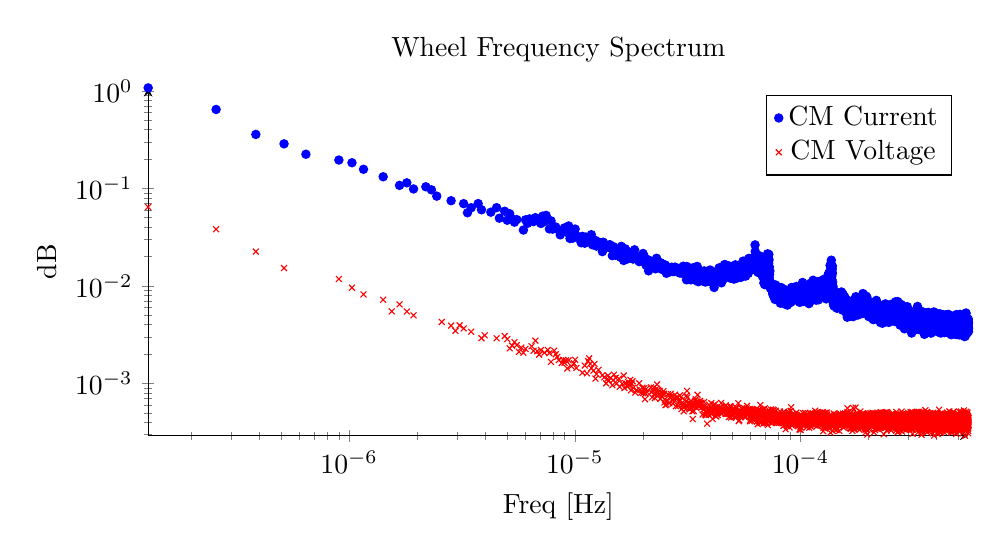
\begin{tikzpicture}
	\begin{loglogaxis}[
		height=6cm,
		width=12cm,
		log basis y=10,
		log basis x=10,
		xlabel={Freq [Hz]},
		ylabel={dB},
		title={Wheel Frequency Spectrum},
		axis x line=bottom,
		axis y line=left,
]
	\addplot[only marks, mark size=1.5pt, color=blue, mark=*] plot coordinates {
		(0.0, 12.9522822218594)
		(1.28600823045268e-07, 1.0710360035539)
		(2.57201646090535e-07, 0.643298683977024)
		(3.85802469135802e-07, 0.357123399202884)
		(5.1440329218107e-07, 0.285862810727382)
		(6.43004115226338e-07, 0.223619256997828)
		(9.00205761316873e-07, 0.195071577903294)
		(1.02880658436214e-06, 0.182936795995074)
		(1.15740740740741e-06, 0.156762101057921)
		(1.41460905349794e-06, 0.131423349892345)
		(1.67181069958848e-06, 0.107242545534043)
		(1.80041152263375e-06, 0.113886172179218)
		(1.92901234567901e-06, 0.09857628287995)
		(2.18621399176955e-06, 0.103756394956059)
		(2.31481481481482e-06, 0.096537206396523)
		(2.44341563786008e-06, 0.083167616112623)
		(2.82921810699589e-06, 0.074644258603763)
		(3.21502057613169e-06, 0.069644635671152)
		(3.34362139917696e-06, 0.056184891845839)
		(3.47222222222222e-06, 0.063227741926978)
		(3.72942386831276e-06, 0.069774317170889)
		(3.85802469135802e-06, 0.060316694478964)
		(4.24382716049383e-06, 0.056957056911341)
		(4.50102880658436e-06, 0.063369609399345)
		(4.62962962962963e-06, 0.049444812431559)
		(4.88683127572017e-06, 0.058250112592489)
		(5.01543209876543e-06, 0.04710993596666)
		(5.1440329218107e-06, 0.054881137270369)
		(5.27263374485597e-06, 0.048581442551761)
		(5.40123456790124e-06, 0.044971766735036)
		(5.5298353909465e-06, 0.04779735653459)
		(5.91563786008231e-06, 0.037362749273871)
		(6.04423868312757e-06, 0.047541001354088)
		(6.17283950617284e-06, 0.043780818730206)
		(6.30144032921811e-06, 0.048607027036069)
		(6.55864197530864e-06, 0.045597086760245)
		(6.68724279835391e-06, 0.050050942464595)
		(7.07304526748971e-06, 0.043628902393856)
		(7.20164609053498e-06, 0.051913340080261)
		(7.33024691358025e-06, 0.045865368523489)
		(7.45884773662552e-06, 0.05281597222997)
		(7.71604938271605e-06, 0.038385334939887)
		(7.84465020576132e-06, 0.046399264863807)
		(7.97325102880659e-06, 0.038177143823658)
		(8.23045267489712e-06, 0.040154755509484)
		(8.48765432098766e-06, 0.037540982849393)
		(8.61625514403292e-06, 0.033357361706239)
		(8.74485596707819e-06, 0.035878331754824)
		(9.00205761316873e-06, 0.039349038874498)
		(9.13065843621399e-06, 0.035632554460269)
		(9.38786008230453e-06, 0.041139952962445)
		(9.5164609053498e-06, 0.030598156741876)
		(9.64506172839506e-06, 0.037053176409897)
		(9.77366255144033e-06, 0.030823429881475)
		(9.9022633744856e-06, 0.034479630095551)
		(1.00308641975309e-05, 0.038261274508724)
		(1.01594650205761e-05, 0.032578697223034)
		(1.05452674897119e-05, 0.029969358860741)
		(1.06738683127572e-05, 0.027675543806756)
		(1.08024691358025e-05, 0.032195316334346)
		(1.09310699588477e-05, 0.028918350205571)
		(1.1059670781893e-05, 0.027381496676967)
		(1.11882716049383e-05, 0.031632589952384)
		(1.13168724279835e-05, 0.028766198566269)
		(1.18312757201646e-05, 0.033501623380439)
		(1.19598765432099e-05, 0.026395587980292)
		(1.23456790123457e-05, 0.029238780313415)
		(1.24742798353909e-05, 0.025568810297843)
		(1.26028806584362e-05, 0.028407819885708)
		(1.31172839506173e-05, 0.026414302153325)
		(1.32458847736626e-05, 0.022447107087203)
		(1.33744855967078e-05, 0.028019450917876)
		(1.36316872427984e-05, 0.026311608046219)
		(1.40174897119342e-05, 0.024892943932339)
		(1.42746913580247e-05, 0.026462270179376)
		(1.45318930041152e-05, 0.024350513117891)
		(1.46604938271605e-05, 0.020406655379354)
		(1.47890946502058e-05, 0.025283229424306)
		(1.50462962962963e-05, 0.02394831837456)
		(1.51748971193416e-05, 0.020623167098715)
		(1.53034979423868e-05, 0.02294865094077)
		(1.56893004115226e-05, 0.020474291686978)
		(1.58179012345679e-05, 0.02347990424245)
		(1.59465020576132e-05, 0.019665895068362)
		(1.60751028806584e-05, 0.02541429863355)
		(1.62037037037037e-05, 0.02343808206941)
		(1.6332304526749e-05, 0.020796896954696)
		(1.64609053497942e-05, 0.01821191441267)
		(1.65895061728395e-05, 0.02095856897987)
		(1.67181069958848e-05, 0.023973949601967)
		(1.684670781893e-05, 0.0199576092737)
		(1.69753086419753e-05, 0.022807320547691)
		(1.71039094650206e-05, 0.018889573603148)
		(1.72325102880658e-05, 0.020230192455107)
		(1.73611111111111e-05, 0.022064329587419)
		(1.78755144032922e-05, 0.019698112703338)
		(1.80041152263374e-05, 0.020735858304865)
		(1.81327160493827e-05, 0.018833976481841)
		(1.8261316872428e-05, 0.020230484050109)
		(1.83899176954733e-05, 0.023437766117815)
		(1.85185185185185e-05, 0.020511664186995)
		(1.86471193415638e-05, 0.019475185257427)
		(1.92901234567901e-05, 0.017716262009361)
		(1.94187242798354e-05, 0.019261003346511)
		(1.96759259259259e-05, 0.018047762249801)
		(1.98045267489712e-05, 0.019334426026952)
		(2.00617283950617e-05, 0.02146711142679)
		(2.03189300411523e-05, 0.019853298891741)
		(2.07047325102881e-05, 0.016229274401704)
		(2.08333333333333e-05, 0.01869586517979)
		(2.09619341563786e-05, 0.017415860213694)
		(2.12191358024691e-05, 0.01426912488032)
		(2.13477366255144e-05, 0.018270399570302)
		(2.14763374485597e-05, 0.016537989807376)
		(2.16049382716049e-05, 0.017652802297545)
		(2.2119341563786e-05, 0.016749985658772)
		(2.27623456790123e-05, 0.014969165135278)
		(2.28909465020576e-05, 0.016558803297894)
		(2.30195473251029e-05, 0.019197302869609)
		(2.31481481481481e-05, 0.015918418562181)
		(2.34053497942387e-05, 0.017646501255528)
		(2.37911522633745e-05, 0.016109549477961)
		(2.39197530864198e-05, 0.017297037893569)
		(2.4048353909465e-05, 0.01577681515855)
		(2.43055555555556e-05, 0.014765421905523)
		(2.44341563786008e-05, 0.016830007518372)
		(2.46913580246914e-05, 0.014827575524449)
		(2.52057613168724e-05, 0.016340332418094)
		(2.53343621399177e-05, 0.01528207155491)
		(2.5462962962963e-05, 0.013467480099111)
		(2.55915637860082e-05, 0.015581565169548)
		(2.63631687242798e-05, 0.013940073164628)
		(2.67489711934156e-05, 0.014710174618611)
		(2.68775720164609e-05, 0.015545310636611)
		(2.70061728395062e-05, 0.014016594648958)
		(2.7391975308642e-05, 0.015264801773861)
		(2.75205761316872e-05, 0.014040667511562)
		(2.77777777777778e-05, 0.015593292302862)
		(2.80349794238683e-05, 0.014241384438788)
		(2.86779835390946e-05, 0.014989864797968)
		(2.90637860082305e-05, 0.013583024021383)
		(2.91923868312757e-05, 0.015114153295482)
		(2.95781893004115e-05, 0.013521380678704)
		(3.02211934156379e-05, 0.015909768015488)
		(3.03497942386831e-05, 0.013434940687219)
		(3.06069958847737e-05, 0.015018540674536)
		(3.07355967078189e-05, 0.013516248932139)
		(3.11213991769547e-05, 0.014279982398967)
		(3.125e-05, 0.011549702985317)
		(3.13786008230453e-05, 0.015792101903251)
		(3.15072016460905e-05, 0.014788633753026)
		(3.16358024691358e-05, 0.011835493620996)
		(3.17644032921811e-05, 0.012617896708039)
		(3.18930041152263e-05, 0.014257125846545)
		(3.25360082304527e-05, 0.012904445902187)
		(3.26646090534979e-05, 0.011538297558915)
		(3.29218106995885e-05, 0.01302829986911)
		(3.30504115226337e-05, 0.013707564523103)
		(3.3179012345679e-05, 0.012003576798169)
		(3.34362139917695e-05, 0.015339262635014)
		(3.36934156378601e-05, 0.012808265173636)
		(3.40792181069959e-05, 0.011575338340213)
		(3.42078189300412e-05, 0.013351916919281)
		(3.43364197530864e-05, 0.011387175631811)
		(3.44650205761317e-05, 0.014572813620536)
		(3.4593621399177e-05, 0.015668104034144)
		(3.47222222222222e-05, 0.013780734097281)
		(3.48508230452675e-05, 0.015828526167747)
		(3.49794238683128e-05, 0.014170482836786)
		(3.52366255144033e-05, 0.011031284616605)
		(3.53652263374486e-05, 0.012578968581416)
		(3.56224279835391e-05, 0.011789490441538)
		(3.60082304526749e-05, 0.013105562069586)
		(3.61368312757202e-05, 0.011533288788059)
		(3.62654320987654e-05, 0.013308711699094)
		(3.66512345679012e-05, 0.011915268218801)
		(3.69084362139918e-05, 0.011241780214262)
		(3.7037037037037e-05, 0.012664891241242)
		(3.71656378600823e-05, 0.013423534264936)
		(3.74228395061728e-05, 0.014248926754214)
		(3.75514403292181e-05, 0.01309598137734)
		(3.78086419753086e-05, 0.010956341228683)
		(3.79372427983539e-05, 0.011795961099461)
		(3.80658436213992e-05, 0.011074810370599)
		(3.81944444444444e-05, 0.011709016102426)
		(3.83230452674897e-05, 0.013446400140999)
		(3.8451646090535e-05, 0.01110640743136)
		(3.85802469135802e-05, 0.012269396318095)
		(3.88374485596708e-05, 0.013672651399745)
		(3.92232510288066e-05, 0.012321658693648)
		(3.93518518518519e-05, 0.013086333322583)
		(3.94804526748971e-05, 0.011102087744131)
		(3.97376543209877e-05, 0.014542468321367)
		(3.98662551440329e-05, 0.013705185029187)
		(3.99948559670782e-05, 0.012511598737008)
		(4.01234567901235e-05, 0.013440237403963)
		(4.0380658436214e-05, 0.011814683146)
		(4.10236625514403e-05, 0.013685171599412)
		(4.12808641975309e-05, 0.012828849924978)
		(4.14094650205761e-05, 0.00963215608648)
		(4.15380658436214e-05, 0.011927499059539)
		(4.17952674897119e-05, 0.01271582564651)
		(4.19238683127572e-05, 0.011196200736757)
		(4.20524691358025e-05, 0.01385330201402)
		(4.21810699588477e-05, 0.013060325503212)
		(4.2309670781893e-05, 0.012371978098226)
		(4.25668724279835e-05, 0.011588775608036)
		(4.29526748971193e-05, 0.013847324809275)
		(4.33384773662551e-05, 0.011822880989143)
		(4.34670781893004e-05, 0.013936868000349)
		(4.35956790123457e-05, 0.015310196069899)
		(4.3724279835391e-05, 0.013579677472504)
		(4.39814814814815e-05, 0.012462942731492)
		(4.41100823045267e-05, 0.013567337948346)
		(4.44958847736625e-05, 0.011531616869706)
		(4.46244855967078e-05, 0.010753680262826)
		(4.47530864197531e-05, 0.01218456578641)
		(4.51388888888889e-05, 0.0134970195479)
		(4.52674897119342e-05, 0.014659891409243)
		(4.53960905349794e-05, 0.011660027395745)
		(4.59104938271605e-05, 0.01354898874916)
		(4.60390946502058e-05, 0.016519943873671)
		(4.6167695473251e-05, 0.014255098759457)
		(4.62962962962963e-05, 0.01627428620352)
		(4.64248971193416e-05, 0.015440785530884)
		(4.65534979423868e-05, 0.016415263977995)
		(4.66820987654321e-05, 0.012517476989592)
		(4.69393004115226e-05, 0.013300750653791)
		(4.71965020576132e-05, 0.01454537312096)
		(4.77109053497942e-05, 0.012495746909203)
		(4.78395061728395e-05, 0.013871828540255)
		(4.82253086419753e-05, 0.015996694422846)
		(4.84825102880658e-05, 0.013606780328065)
		(4.86111111111111e-05, 0.012718969038893)
		(4.87397119341564e-05, 0.015460683734707)
		(4.89969135802469e-05, 0.011982042276393)
		(4.91255144032922e-05, 0.014592932195413)
		(4.93827160493827e-05, 0.013145770934726)
		(4.96399176954732e-05, 0.014010348608913)
		(4.98971193415638e-05, 0.012114296186002)
		(5.00257201646091e-05, 0.013729149517753)
		(5.01543209876543e-05, 0.012520633181419)
		(5.06687242798354e-05, 0.011729526063995)
		(5.07973251028807e-05, 0.012743055344487)
		(5.10545267489712e-05, 0.015129537756669)
		(5.11831275720165e-05, 0.013146873116405)
		(5.13117283950617e-05, 0.014201783897258)
		(5.1440329218107e-05, 0.016438077701661)
		(5.15689300411523e-05, 0.012656041062546)
		(5.18261316872428e-05, 0.011914466794904)
		(5.19547325102881e-05, 0.012929788625477)
		(5.22119341563786e-05, 0.013935020658342)
		(5.23405349794239e-05, 0.013082004685655)
		(5.24691358024691e-05, 0.015628503762041)
		(5.25977366255144e-05, 0.01244176240233)
		(5.27263374485597e-05, 0.015690226919342)
		(5.29835390946502e-05, 0.013593442056437)
		(5.3369341563786e-05, 0.0128068463302)
		(5.34979423868313e-05, 0.014819467105223)
		(5.38837448559671e-05, 0.012563026747344)
		(5.40123456790123e-05, 0.013700829532123)
		(5.42695473251029e-05, 0.012983960754515)
		(5.43981481481482e-05, 0.01221890057071)
		(5.45267489711934e-05, 0.01396367871559)
		(5.46553497942387e-05, 0.01537943016044)
		(5.50411522633745e-05, 0.016770326303898)
		(5.51697530864198e-05, 0.015908998074097)
		(5.5298353909465e-05, 0.015054538386274)
		(5.54269547325103e-05, 0.016690762159235)
		(5.55555555555556e-05, 0.015635742588878)
		(5.56841563786008e-05, 0.017952883747987)
		(5.59413580246914e-05, 0.016193994015956)
		(5.61985596707819e-05, 0.01372888528257)
		(5.65843621399177e-05, 0.015109781256956)
		(5.6712962962963e-05, 0.014033553368593)
		(5.68415637860082e-05, 0.015501363211486)
		(5.70987654320988e-05, 0.012588226580566)
		(5.7227366255144e-05, 0.013682977480116)
		(5.73559670781893e-05, 0.016265930028509)
		(5.76131687242798e-05, 0.01482745538437)
		(5.77417695473251e-05, 0.015997005719703)
		(5.79989711934156e-05, 0.018250599110732)
		(5.81275720164609e-05, 0.015531600741966)
		(5.82561728395062e-05, 0.013546118968111)
		(5.83847736625514e-05, 0.015534557746597)
		(5.85133744855967e-05, 0.016388767964879)
		(5.8641975308642e-05, 0.013404671636404)
		(5.87705761316872e-05, 0.01450118156095)
		(5.88991769547325e-05, 0.015940178229241)
		(5.90277777777778e-05, 0.019139952748305)
		(5.9156378600823e-05, 0.017080535541281)
		(5.96707818930041e-05, 0.019021398001314)
		(5.97993827160494e-05, 0.015396598143653)
		(6.01851851851852e-05, 0.014528388820871)
		(6.06995884773663e-05, 0.016241862400226)
		(6.08281893004115e-05, 0.018392598977999)
		(6.09567901234568e-05, 0.014797954843991)
		(6.10853909465021e-05, 0.017267315071063)
		(6.12139917695473e-05, 0.015964592665508)
		(6.14711934156379e-05, 0.019342001848884)
		(6.15997942386831e-05, 0.016851912609151)
		(6.17283950617284e-05, 0.014828707950345)
		(6.18569958847737e-05, 0.018230272524139)
		(6.19855967078189e-05, 0.01591226513573)
		(6.21141975308642e-05, 0.01716891007434)
		(6.22427983539095e-05, 0.015647990803898)
		(6.23713991769547e-05, 0.016892840098812)
		(6.25e-05, 0.018255477640777)
		(6.28858024691358e-05, 0.026316865083392)
		(6.30144032921811e-05, 0.022496712548059)
		(6.31430041152263e-05, 0.020243129094367)
		(6.36574074074074e-05, 0.01784962841948)
		(6.39146090534979e-05, 0.01879805996284)
		(6.40432098765432e-05, 0.016189050089923)
		(6.41718106995885e-05, 0.014818891654894)
		(6.43004115226337e-05, 0.016937426067498)
		(6.45576131687243e-05, 0.015804986187868)
		(6.48148148148148e-05, 0.013791738169298)
		(6.49434156378601e-05, 0.01560253025651)
		(6.50720164609054e-05, 0.013735371630288)
		(6.52006172839506e-05, 0.01450151263374)
		(6.53292181069959e-05, 0.015560781308234)
		(6.54578189300412e-05, 0.018172051944061)
		(6.55864197530864e-05, 0.020042990307715)
		(6.57150205761317e-05, 0.018724037172549)
		(6.59722222222222e-05, 0.020290673844316)
		(6.61008230452675e-05, 0.016182689324357)
		(6.62294238683128e-05, 0.018549047585939)
		(6.6358024691358e-05, 0.017387108740061)
		(6.64866255144033e-05, 0.019028578566825)
		(6.66152263374486e-05, 0.015813635920478)
		(6.68724279835391e-05, 0.013971533516032)
		(6.71296296296296e-05, 0.01489905927743)
		(6.72582304526749e-05, 0.013997497966825)
		(6.75154320987654e-05, 0.01293367756724)
		(6.76440329218107e-05, 0.014191549649705)
		(6.7772633744856e-05, 0.01259542825393)
		(6.79012345679012e-05, 0.016518631427044)
		(6.80298353909465e-05, 0.013326971277901)
		(6.8287037037037e-05, 0.014084770428959)
		(6.84156378600823e-05, 0.013144733533814)
		(6.88014403292181e-05, 0.010699710605441)
		(6.89300411522634e-05, 0.011627632361079)
		(6.91872427983539e-05, 0.013958805794903)
		(6.94444444444444e-05, 0.010300525063703)
		(6.95730452674897e-05, 0.011887713154893)
		(6.9701646090535e-05, 0.014781052344327)
		(6.98302469135802e-05, 0.01247722375369)
		(6.99588477366255e-05, 0.013371646476312)
		(7.04732510288066e-05, 0.014917105666162)
		(7.06018518518519e-05, 0.016453708137862)
		(7.09876543209877e-05, 0.018565413407054)
		(7.11162551440329e-05, 0.013993876769048)
		(7.12448559670782e-05, 0.014960864657442)
		(7.13734567901235e-05, 0.02012161072258)
		(7.15020576131687e-05, 0.021330115931706)
		(7.1630658436214e-05, 0.019803197347746)
		(7.18878600823045e-05, 0.015830663189929)
		(7.21450617283951e-05, 0.0190233833934)
		(7.22736625514403e-05, 0.017084839453739)
		(7.24022633744856e-05, 0.02103058189791)
		(7.25308641975309e-05, 0.018440533188452)
		(7.26594650205761e-05, 0.012196274115293)
		(7.27880658436214e-05, 0.015622062362894)
		(7.29166666666667e-05, 0.013081956904394)
		(7.31738683127572e-05, 0.014186835838299)
		(7.33024691358025e-05, 0.011120112056151)
		(7.34310699588477e-05, 0.01051098902127)
		(7.3559670781893e-05, 0.009446521314865)
		(7.36882716049383e-05, 0.010028077438993)
		(7.38168724279835e-05, 0.01072763471073)
		(7.43312757201646e-05, 0.009686339922049)
		(7.51028806584362e-05, 0.008740723140962)
		(7.53600823045268e-05, 0.008221747089813)
		(7.5488683127572e-05, 0.008967876520108)
		(7.57458847736625e-05, 0.008410058014113)
		(7.60030864197531e-05, 0.009469353249669)
		(7.61316872427984e-05, 0.010192165363458)
		(7.62602880658436e-05, 0.007729040440737)
		(7.63888888888889e-05, 0.009980549810633)
		(7.65174897119342e-05, 0.008725405308316)
		(7.66460905349794e-05, 0.010041842610524)
		(7.690329218107e-05, 0.008454867127446)
		(7.71604938271605e-05, 0.007252349313627)
		(7.72890946502058e-05, 0.008835331684132)
		(7.7417695473251e-05, 0.008345280313628)
		(7.75462962962963e-05, 0.010220167417201)
		(7.76748971193416e-05, 0.008590522923713)
		(7.78034979423868e-05, 0.009039125668285)
		(7.79320987654321e-05, 0.008298706790408)
		(7.80606995884774e-05, 0.009196230536073)
		(7.84465020576132e-05, 0.009896836473288)
		(7.85751028806584e-05, 0.008357325385464)
		(7.90895061728395e-05, 0.007203115235095)
		(7.92181069958848e-05, 0.008347457854995)
		(7.98611111111111e-05, 0.007625179718742)
		(8.01183127572017e-05, 0.00721803879182)
		(8.03755144032922e-05, 0.008671759697186)
		(8.10185185185185e-05, 0.007857220379301)
		(8.1275720164609e-05, 0.007100085896647)
		(8.14043209876543e-05, 0.006653447674302)
		(8.15329218106996e-05, 0.007587364801324)
		(8.19187242798354e-05, 0.007148321426009)
		(8.20473251028807e-05, 0.009626316011585)
		(8.21759259259259e-05, 0.008346032173701)
		(8.23045267489712e-05, 0.007589733613057)
		(8.24331275720165e-05, 0.008599409881184)
		(8.25617283950617e-05, 0.007504381210528)
		(8.28189300411523e-05, 0.006959951636753)
		(8.29475308641975e-05, 0.008666665249532)
		(8.30761316872428e-05, 0.007506885943573)
		(8.34619341563786e-05, 0.008197672494363)
		(8.37191358024691e-05, 0.007622873594805)
		(8.38477366255144e-05, 0.008367011092776)
		(8.39763374485597e-05, 0.009228024230524)
		(8.41049382716049e-05, 0.007617464337835)
		(8.42335390946502e-05, 0.006582262965168)
		(8.43621399176955e-05, 0.007690406916785)
		(8.44907407407407e-05, 0.008459173043355)
		(8.4619341563786e-05, 0.007569595059322)
		(8.47479423868313e-05, 0.00673165140737)
		(8.48765432098766e-05, 0.007975455556591)
		(8.50051440329218e-05, 0.008382812201069)
		(8.51337448559671e-05, 0.009113963417519)
		(8.52623456790123e-05, 0.008004091348664)
		(8.56481481481482e-05, 0.007473967285583)
		(8.6548353909465e-05, 0.007948475929198)
		(8.66769547325103e-05, 0.008995777602902)
		(8.68055555555556e-05, 0.007551757763811)
		(8.70627572016461e-05, 0.008144802913152)
		(8.71913580246914e-05, 0.007598171279483)
		(8.74485596707819e-05, 0.006357594076256)
		(8.75771604938272e-05, 0.00813081947608)
		(8.80915637860082e-05, 0.007557120029343)
		(8.86059670781893e-05, 0.008088380798133)
		(8.87345679012346e-05, 0.006851366987186)
		(8.89917695473251e-05, 0.0080277199897)
		(8.91203703703704e-05, 0.00716556606684)
		(8.92489711934156e-05, 0.00673828467907)
		(8.95061728395062e-05, 0.007254049820682)
		(8.9891975308642e-05, 0.00779809370752)
		(9.00205761316872e-05, 0.007405009040929)
		(9.01491769547325e-05, 0.006849621893054)
		(9.02777777777778e-05, 0.008085088323262)
		(9.05349794238683e-05, 0.006768687430171)
		(9.06635802469136e-05, 0.007256464169074)
		(9.09207818930041e-05, 0.007981082965589)
		(9.10493827160494e-05, 0.007343157256096)
		(9.11779835390947e-05, 0.007811144393706)
		(9.13065843621399e-05, 0.00962964340412)
		(9.14351851851852e-05, 0.008640612671615)
		(9.15637860082305e-05, 0.008171086981054)
		(9.1820987654321e-05, 0.008685803658995)
		(9.20781893004115e-05, 0.008246323828196)
		(9.22067901234568e-05, 0.007297187377481)
		(9.24639917695473e-05, 0.008264562107172)
		(9.27211934156379e-05, 0.007635937494909)
		(9.28497942386831e-05, 0.008363311890879)
		(9.29783950617284e-05, 0.007159602814162)
		(9.31069958847737e-05, 0.007946205834624)
		(9.32355967078189e-05, 0.008433807884836)
		(9.33641975308642e-05, 0.009189237192939)
		(9.34927983539095e-05, 0.007177301544492)
		(9.375e-05, 0.007738316439135)
		(9.38786008230453e-05, 0.008617443256048)
		(9.41358024691358e-05, 0.009189186994946)
		(9.42644032921811e-05, 0.008057899105028)
		(9.46502057613169e-05, 0.007581413748964)
		(9.47788065843621e-05, 0.008023992400037)
		(9.50360082304527e-05, 0.007547930217063)
		(9.5164609053498e-05, 0.008447909980917)
		(9.52932098765432e-05, 0.007925553639794)
		(9.54218106995885e-05, 0.007180488815049)
		(9.55504115226337e-05, 0.00815541843431)
		(9.5679012345679e-05, 0.009859383762141)
		(9.58076131687243e-05, 0.008041192845234)
		(9.61934156378601e-05, 0.00738795205303)
		(9.63220164609053e-05, 0.00783325693889)
		(9.64506172839506e-05, 0.007216514368434)
		(9.68364197530864e-05, 0.008179113553158)
		(9.7093621399177e-05, 0.008704953258931)
		(9.72222222222222e-05, 0.007844614580568)
		(9.74794238683128e-05, 0.008902874241851)
		(9.7608024691358e-05, 0.007903897412747)
		(9.78652263374486e-05, 0.007395104056597)
		(9.79938271604938e-05, 0.008472015956632)
		(9.85082304526749e-05, 0.007941050600274)
		(9.86368312757202e-05, 0.009436900803647)
		(9.87654320987654e-05, 0.008695295939625)
		(9.88940329218107e-05, 0.007358825025689)
		(9.9022633744856e-05, 0.007843952020245)
		(9.91512345679012e-05, 0.008929713796581)
		(9.92798353909465e-05, 0.006776509624412)
		(9.9537037037037e-05, 0.007594003483525)
		(9.96656378600823e-05, 0.00856620501134)
		(0.000100308641975, 0.007849509503733)
		(0.000100437242798, 0.008919417438214)
		(0.000100565843621, 0.007809698258861)
		(0.000100694444444, 0.009045919698937)
		(0.000100823045267, 0.008334571743306)
		(0.000101208847737, 0.009417288104604)
		(0.00010133744856, 0.008123470140003)
		(0.000101466049383, 0.009405230106269)
		(0.000101594650206, 0.008919692485136)
		(0.000101851851852, 0.009414688030111)
		(0.000102109053498, 0.010835401429888)
		(0.000102237654321, 0.007860641342288)
		(0.000102366255144, 0.008560288038549)
		(0.000102494855967, 0.009125340324753)
		(0.000102752057613, 0.007632505304925)
		(0.000102880658436, 0.008654159982107)
		(0.000103266460905, 0.006929217969547)
		(0.000103395061728, 0.00752436053468)
		(0.000103780864198, 0.008261565346326)
		(0.000103909465021, 0.007778436534616)
		(0.000104038065844, 0.00889814451051)
		(0.00010429526749, 0.009514761502277)
		(0.000104423868313, 0.008863667506327)
		(0.000104552469136, 0.007931286643985)
		(0.000104681069959, 0.008637394319151)
		(0.000104938271605, 0.007534334590379)
		(0.000105452674897, 0.008688765156557)
		(0.00010558127572, 0.009150600933592)
		(0.000105838477366, 0.008441069583945)
		(0.000106095679012, 0.007668168019355)
		(0.000106224279835, 0.008376927248123)
		(0.000106481481481, 0.006912712662725)
		(0.000106610082305, 0.008831552183672)
		(0.000106867283951, 0.007664843377455)
		(0.000106995884774, 0.008376162983411)
		(0.000107124485597, 0.007882050933192)
		(0.00010725308642, 0.007481658541504)
		(0.000107510288066, 0.009078800826514)
		(0.000107638888889, 0.008602556295355)
		(0.000107767489712, 0.007433253961907)
		(0.000107896090535, 0.008939409247281)
		(0.000108024691358, 0.008120723490727)
		(0.00010853909465, 0.00687581279512)
		(0.000108924897119, 0.008196780093066)
		(0.000109053497942, 0.006578251290123)
		(0.000109182098765, 0.00719451568021)
		(0.000109567901235, 0.007666835352601)
		(0.000109696502058, 0.009545992582253)
		(0.000109825102881, 0.007716316110778)
		(0.000109953703704, 0.008848843761066)
		(0.000110082304527, 0.010047752121657)
		(0.00011021090535, 0.010574694758924)
		(0.000110339506173, 0.009023514222399)
		(0.000110725308642, 0.009880701361976)
		(0.000110853909465, 0.008990918671667)
		(0.000110982510288, 0.00808471400035)
		(0.000111111111111, 0.0070993285793)
		(0.000111239711934, 0.008117343750546)
		(0.000111368312757, 0.009457754120264)
		(0.000111625514403, 0.008934663511495)
		(0.000111882716049, 0.007926218855991)
		(0.000112011316872, 0.008559274599686)
		(0.000112139917695, 0.00918928569851)
		(0.000112268518519, 0.008043915712867)
		(0.000112397119342, 0.009125190351823)
		(0.000112525720165, 0.007355992789727)
		(0.000112654320988, 0.008093097458158)
		(0.000112782921811, 0.007139494967961)
		(0.000113040123457, 0.009060419981757)
		(0.00011316872428, 0.009580043086415)
		(0.000113297325103, 0.010127841509705)
		(0.000113425925926, 0.009168539838528)
		(0.000113554526749, 0.008104127260732)
		(0.000113683127572, 0.011422966411873)
		(0.000113811728395, 0.009558684415754)
		(0.000113940329218, 0.008991191417597)
		(0.000114326131687, 0.009780045084143)
		(0.00011445473251, 0.008201107817051)
		(0.000114711934156, 0.009175322543831)
		(0.000114840534979, 0.010747997248828)
		(0.000114969135802, 0.009610765971354)
		(0.000115097736626, 0.010464490940594)
		(0.000115354938272, 0.009401743722886)
		(0.000115483539095, 0.008565781563965)
		(0.000115612139918, 0.009369719464843)
		(0.000115869341564, 0.007897785786461)
		(0.000115997942387, 0.008305728963743)
		(0.000116255144033, 0.00880246274198)
		(0.000116383744856, 0.00935703758462)
		(0.000116898148148, 0.007933825899423)
		(0.000117026748971, 0.009128167467212)
		(0.000117283950617, 0.007140318727841)
		(0.00011741255144, 0.007624273537306)
		(0.000117541152263, 0.008188298939937)
		(0.000117669753086, 0.009237792859999)
		(0.000117798353909, 0.007261807049944)
		(0.000117926954733, 0.00939630804246)
		(0.000118184156379, 0.008746646120629)
		(0.000118312757202, 0.009411547697808)
		(0.000118441358025, 0.010601324106913)
		(0.000118827160494, 0.008495093179832)
		(0.000118955761317, 0.010069326388621)
		(0.000119341563786, 0.011058157037129)
		(0.000119470164609, 0.00875278517782)
		(0.000119598765432, 0.007377262474514)
		(0.000119727366255, 0.008287448415993)
		(0.000119855967078, 0.009042479435223)
		(0.000120113168724, 0.007198216388358)
		(0.000120241769547, 0.008698603060653)
		(0.00012037037037, 0.010477948279753)
		(0.000120498971193, 0.009798088868743)
		(0.00012075617284, 0.008793434493009)
		(0.000121141975309, 0.009308667032912)
		(0.000121270576132, 0.010120102306136)
		(0.000121399176955, 0.010958094716249)
		(0.000121527777778, 0.009688937027183)
		(0.000121656378601, 0.010233293047561)
		(0.000121913580247, 0.008698961560648)
		(0.000122170781893, 0.010849424835921)
		(0.000122299382716, 0.009562626642732)
		(0.000122556584362, 0.009039551116905)
		(0.000122685185185, 0.010165999136458)
		(0.000122942386831, 0.009115120586753)
		(0.000123199588477, 0.008335585093071)
		(0.0001233281893, 0.010132384035013)
		(0.000123456790123, 0.010751654341534)
		(0.00012371399177, 0.009706074767712)
		(0.000123971193416, 0.010492172842478)
		(0.000124099794239, 0.009608338691783)
		(0.000124356995885, 0.00910280175503)
		(0.000124742798354, 0.007876404551113)
		(0.000124871399177, 0.008715335221714)
		(0.000125257201646, 0.009331879677814)
		(0.000125514403292, 0.01091532971446)
		(0.000125771604938, 0.008861977644853)
		(0.000125900205761, 0.010441468645241)
		(0.000126028806584, 0.011583419556155)
		(0.000126157407407, 0.008580641454071)
		(0.00012628600823, 0.009155381028653)
		(0.000126543209877, 0.008681050289339)
		(0.0001266718107, 0.009543920533683)
		(0.000126929012346, 0.008884959595566)
		(0.000127057613169, 0.008120051345398)
		(0.000127186213992, 0.009076180468692)
		(0.000127314814815, 0.011370424947939)
		(0.000127443415638, 0.009989384799245)
		(0.000127829218107, 0.009382939325338)
		(0.00012795781893, 0.010427946653275)
		(0.000128086419753, 0.009457867412133)
		(0.000128343621399, 0.008646923915785)
		(0.000128729423868, 0.009256819261733)
		(0.000128986625514, 0.008723338058302)
		(0.000129501028807, 0.009308499490657)
		(0.00012962962963, 0.008523206242998)
		(0.000129886831276, 0.007355432216313)
		(0.000130015432099, 0.008530448537227)
		(0.000130272633745, 0.010045404986563)
		(0.000130401234568, 0.010773270920441)
		(0.000130529835391, 0.009166315571259)
		(0.000130658436214, 0.010269935589546)
		(0.000131172839506, 0.008521537699283)
		(0.000131301440329, 0.009760615493832)
		(0.000131558641975, 0.010556132251961)
		(0.000131687242798, 0.0097593844162)
		(0.000131944444444, 0.010789843296604)
		(0.000132073045267, 0.011626284889743)
		(0.000132201646091, 0.012783981730799)
		(0.000132330246914, 0.012111470103054)
		(0.000133359053498, 0.013457743281633)
		(0.000133487654321, 0.012451490971541)
		(0.00013387345679, 0.010919945146495)
		(0.000134002057613, 0.009479096567034)
		(0.000134259259259, 0.011024292519372)
		(0.000134387860082, 0.012244000865241)
		(0.000134645061728, 0.009981230212694)
		(0.000134773662551, 0.011967008115025)
		(0.000135030864198, 0.00990243582239)
		(0.000135159465021, 0.013760872797475)
		(0.000135288065844, 0.016273867619239)
		(0.000135416666667, 0.014310627854773)
		(0.000135802469136, 0.012473980527023)
		(0.000135931069959, 0.013718454097546)
		(0.000136059670782, 0.015746370285344)
		(0.000136188271605, 0.016649954437723)
		(0.000136316872428, 0.014287497302478)
		(0.000136445473251, 0.013359169743074)
		(0.00013683127572, 0.015627443836476)
		(0.000136959876543, 0.018340378798969)
		(0.000137088477366, 0.01436574733008)
		(0.000137602880658, 0.012575579868354)
		(0.000137731481481, 0.011610381845595)
		(0.000137860082305, 0.010591458851444)
		(0.000137988683128, 0.013434848592743)
		(0.000138117283951, 0.015987038248814)
		(0.000138245884774, 0.014844986341532)
		(0.000138374485597, 0.015968810913807)
		(0.00013850308642, 0.013550005721923)
		(0.000138760288066, 0.010947158786307)
		(0.000138888888889, 0.008693161325847)
		(0.000139017489712, 0.009711247293703)
		(0.000139146090535, 0.009170438694138)
		(0.000139274691358, 0.009887724100726)
		(0.000139531893004, 0.007809235850521)
		(0.000139660493827, 0.008323679348441)
		(0.00013978909465, 0.006961120173116)
		(0.000139917695473, 0.006517985238398)
		(0.000140046296296, 0.007687695514368)
		(0.000140174897119, 0.006967784085456)
		(0.000140560699588, 0.006232580580571)
		(0.000140689300412, 0.007710887264384)
		(0.000140817901235, 0.006696291683479)
		(0.000140946502058, 0.007350694312813)
		(0.000141075102881, 0.006300241508241)
		(0.000141203703704, 0.007440251475225)
		(0.000141332304527, 0.008145150041723)
		(0.00014146090535, 0.007695608747405)
		(0.000141589506173, 0.008281567794327)
		(0.000141846707819, 0.007363644890426)
		(0.000141975308642, 0.008794902452597)
		(0.000142103909465, 0.007057456889045)
		(0.000142232510288, 0.006466432225217)
		(0.000142489711934, 0.007297636472809)
		(0.000142875514403, 0.007763947544535)
		(0.000143004115226, 0.006619311567513)
		(0.000143261316872, 0.007195644091064)
		(0.000143518518519, 0.008016379805703)
		(0.000143647119342, 0.006056329934031)
		(0.000143775720165, 0.006911238896798)
		(0.000143904320988, 0.007674158367773)
		(0.000144032921811, 0.006209723682354)
		(0.000144161522634, 0.007543603425772)
		(0.00014441872428, 0.008085977308324)
		(0.000144547325103, 0.006366590829426)
		(0.000144675925926, 0.006835001608774)
		(0.000145061728395, 0.005898522429179)
		(0.000145190329218, 0.007690514123425)
		(0.000145318930041, 0.006054604570715)
		(0.000145447530864, 0.007465213870852)
		(0.00014570473251, 0.006459411386922)
		(0.000145961934156, 0.007073231449078)
		(0.000146090534979, 0.006159286488599)
		(0.000146219135802, 0.00676857173601)
		(0.000146347736626, 0.007267491722543)
		(0.000146604938272, 0.006318783031252)
		(0.000146862139918, 0.006992852571304)
		(0.000147119341564, 0.00752142759775)
		(0.000147247942387, 0.006827202245816)
		(0.000147762345679, 0.00767280252866)
		(0.000148148148148, 0.00691003610069)
		(0.000148533950617, 0.007371499381537)
		(0.000148919753086, 0.00635485678142)
		(0.000149048353909, 0.007603446552097)
		(0.000149176954733, 0.006917921492944)
		(0.000149305555556, 0.007438135853842)
		(0.000149434156379, 0.007917252676951)
		(0.000149562757202, 0.007180143760923)
		(0.000149691358025, 0.006171975766357)
		(0.000149819958848, 0.007878460146957)
		(0.000149948559671, 0.007467522781071)
		(0.00015033436214, 0.006737809636343)
		(0.000150462962963, 0.007318654806689)
		(0.000150848765432, 0.008475724065817)
		(0.000151234567901, 0.008026455670248)
		(0.000151491769547, 0.008594171342556)
		(0.000151748971193, 0.007785027676697)
		(0.00015200617284, 0.008654205982657)
		(0.000152134773663, 0.007788509134684)
		(0.000153034979424, 0.006631278509887)
		(0.000153163580247, 0.006189086596352)
		(0.00015329218107, 0.00701401224774)
		(0.000153420781893, 0.006547860363261)
		(0.000153549382716, 0.005641588135751)
		(0.000153677983539, 0.006664997747274)
		(0.000153806584362, 0.00613032546252)
		(0.000153935185185, 0.006759752170803)
		(0.000154192386831, 0.006285806852354)
		(0.000154320987654, 0.008212127507893)
		(0.000154449588477, 0.007296608849268)
		(0.000154706790123, 0.007686234088025)
		(0.000154835390947, 0.006469846210836)
		(0.00015496399177, 0.005673247007359)
		(0.000155349794239, 0.006774143568695)
		(0.000155606995885, 0.007292479239079)
		(0.000155735596708, 0.006038395469956)
		(0.000155864197531, 0.006949347467854)
		(0.000155992798354, 0.005882295806971)
		(0.000156121399177, 0.006514113107144)
		(0.00015625, 0.0061035544515)
		(0.000156378600823, 0.006824888899145)
		(0.000156507201646, 0.007230187239129)
		(0.000156764403292, 0.006247473888901)
		(0.000156893004115, 0.007746579108369)
		(0.000157021604938, 0.006714709098326)
		(0.00015753600823, 0.007464066082918)
		(0.000157793209877, 0.006915835826218)
		(0.0001579218107, 0.005945040706655)
		(0.000158050411523, 0.006421312147399)
		(0.000158436213992, 0.005677523810871)
		(0.000158950617284, 0.00612255584981)
		(0.000159079218107, 0.005438231454866)
		(0.00015920781893, 0.005756142784276)
		(0.000159336419753, 0.006424445830491)
		(0.000159465020576, 0.005470616671229)
		(0.000159593621399, 0.006232545424154)
		(0.000159850823045, 0.005809266462053)
		(0.000160108024691, 0.005214211093623)
		(0.000160365226337, 0.005589261854579)
		(0.00016049382716, 0.006487724456019)
		(0.00016087962963, 0.005610343699629)
		(0.000161008230453, 0.00504429791281)
		(0.000161136831276, 0.004772536845848)
		(0.000161265432099, 0.005744871624963)
		(0.000161394032922, 0.006280002905383)
		(0.000161651234568, 0.00667292268938)
		(0.000161908436214, 0.005717508627851)
		(0.00016216563786, 0.006716280281329)
		(0.000162551440329, 0.006000749733243)
		(0.000162808641975, 0.007067990486333)
		(0.000162937242798, 0.005940762611703)
		(0.000163065843621, 0.006658587396716)
		(0.000163194444444, 0.005743449820041)
		(0.000163323045267, 0.006496688871221)
		(0.000163451646091, 0.005975439222708)
		(0.00016383744856, 0.005285295706991)
		(0.000163966049383, 0.005893260106409)
		(0.000164094650206, 0.006767795153947)
		(0.000164351851852, 0.006070380648028)
		(0.000164480452675, 0.005313996816398)
		(0.000164609053498, 0.006767386869733)
		(0.000164737654321, 0.005451492087342)
		(0.000164866255144, 0.006492075218701)
		(0.000164994855967, 0.005434147099656)
		(0.000165252057613, 0.006204188674821)
		(0.000165380658436, 0.005847138171937)
		(0.000165637860082, 0.004888237919419)
		(0.000165766460905, 0.006010490776578)
		(0.000165895061728, 0.005463931036896)
		(0.000166023662551, 0.004891311759438)
		(0.000166280864198, 0.005180853259212)
		(0.000166409465021, 0.006159631448319)
		(0.000166538065844, 0.005762188356498)
		(0.00016679526749, 0.006599711985046)
		(0.000166923868313, 0.005295474612832)
		(0.000167438271605, 0.006527577807158)
		(0.000167566872428, 0.005838723285426)
		(0.000167695473251, 0.006520410356956)
		(0.000167824074074, 0.006094035883509)
		(0.000167952674897, 0.005593972452013)
		(0.00016808127572, 0.005138377951142)
		(0.000168209876543, 0.006240573055738)
		(0.000168467078189, 0.004930152345626)
		(0.000168595679012, 0.005620265644282)
		(0.000168724279835, 0.005157285477573)
		(0.000169110082305, 0.005654987444104)
		(0.000169238683128, 0.006369775142849)
		(0.000169367283951, 0.005852690022836)
		(0.00016975308642, 0.00540705841386)
		(0.000169881687243, 0.005116094454201)
		(0.000170138888889, 0.005468520693217)
		(0.000170267489712, 0.005880675848832)
		(0.000170396090535, 0.006844304369161)
		(0.000170524691358, 0.00550910431308)
		(0.000170653292181, 0.005896574809716)
		(0.000170781893004, 0.006206723842999)
		(0.000171167695473, 0.00680289207046)
		(0.000171296296296, 0.004842998236916)
		(0.000171424897119, 0.005817907242594)
		(0.000172582304527, 0.00672363214831)
		(0.00017271090535, 0.007089227583202)
		(0.000172839506173, 0.00629093246407)
		(0.000173225308642, 0.005029366759547)
		(0.000173353909465, 0.005711673994596)
		(0.000173482510288, 0.006018010560479)
		(0.000173611111111, 0.00566434180495)
		(0.000173868312757, 0.006265678658651)
		(0.00017399691358, 0.005912751693256)
		(0.000174254115226, 0.006285117604896)
		(0.000174382716049, 0.006668615877204)
		(0.000174768518519, 0.007362139047837)
		(0.000174897119342, 0.006747537195519)
		(0.000175282921811, 0.005541258355263)
		(0.000175411522634, 0.006814891758147)
		(0.000175797325103, 0.006451640460865)
		(0.000175925925926, 0.007750526609802)
		(0.000176054526749, 0.006298901311569)
		(0.000176311728395, 0.005556095448321)
		(0.000176440329218, 0.006569770198311)
		(0.000176568930041, 0.006227598100468)
		(0.000176697530864, 0.007296772902575)
		(0.00017695473251, 0.00658956646276)
		(0.000177211934156, 0.005894516553566)
		(0.000177340534979, 0.007135423649778)
		(0.000177469135802, 0.007611515520648)
		(0.000177597736626, 0.006951253056195)
		(0.000177726337449, 0.00607518561941)
		(0.000177854938272, 0.005445061219654)
		(0.000177983539095, 0.00616492330756)
		(0.000178112139918, 0.006641806198803)
		(0.000178369341564, 0.005974463890251)
		(0.00017862654321, 0.006716570808699)
		(0.000178755144033, 0.006332989747015)
		(0.000178883744856, 0.005980492188778)
		(0.000179012345679, 0.00558415621947)
		(0.000179140946502, 0.006303894965988)
		(0.000179269547325, 0.005442193964504)
		(0.000179398148148, 0.005993933784108)
		(0.000179783950617, 0.005028025245536)
		(0.000180041152263, 0.005831469542608)
		(0.000180169753086, 0.006552860733147)
		(0.000180298353909, 0.005986328325279)
		(0.000180426954733, 0.005434899615568)
		(0.000180555555556, 0.005987559455341)
		(0.000180684156379, 0.006802685127291)
		(0.000180812757202, 0.005573813521553)
		(0.000180941358025, 0.00638202573993)
		(0.000181198559671, 0.005982514128458)
		(0.000181712962963, 0.006343526995845)
		(0.000181841563786, 0.006879427305426)
		(0.000181970164609, 0.006362055238498)
		(0.000182098765432, 0.005405467146162)
		(0.000182227366255, 0.006149900008429)
		(0.00018287037037, 0.005524903897723)
		(0.000182998971193, 0.006051747966326)
		(0.000183127572016, 0.00713233583674)
		(0.000183384773663, 0.005696298400013)
		(0.000183513374486, 0.006784913806571)
		(0.000183641975309, 0.006202887633969)
		(0.000183770576132, 0.005611297640135)
		(0.000183899176955, 0.006221836966826)
		(0.00018454218107, 0.005704203745578)
		(0.000184670781893, 0.006085213718413)
		(0.000184927983539, 0.005679825138511)
		(0.000185056584362, 0.006203465835609)
		(0.000185185185185, 0.005781118916433)
		(0.000186728395062, 0.006755166704331)
		(0.000186856995885, 0.005503932103099)
		(0.000187114197531, 0.006064174361231)
		(0.000187242798354, 0.006535486852849)
		(0.000187371399177, 0.005969439673101)
		(0.0001875, 0.005205744434525)
		(0.000187628600823, 0.005891367581388)
		(0.000187885802469, 0.007312243621346)
		(0.000188271604938, 0.005717834515142)
		(0.000188400205761, 0.0052503218069)
		(0.000188528806584, 0.006566717910629)
		(0.0001891718107, 0.008339709898462)
		(0.000189300411523, 0.006527342565084)
		(0.000189429012346, 0.005900380041887)
		(0.000189557613169, 0.006532075578732)
		(0.000189686213992, 0.006131840128841)
		(0.000189814814815, 0.007319492289647)
		(0.000189943415638, 0.006257594658301)
		(0.000190586419753, 0.007518439137683)
		(0.000190715020576, 0.006607563526797)
		(0.000190843621399, 0.005742297497332)
		(0.000190972222222, 0.006856272546004)
		(0.000191229423868, 0.005949787541942)
		(0.000191358024691, 0.006324715018979)
		(0.000191615226337, 0.00694249075567)
		(0.00019174382716, 0.006533902186134)
		(0.000191872427984, 0.005662612111995)
		(0.000192001028807, 0.006447457163176)
		(0.00019212962963, 0.00572498160228)
		(0.000192258230453, 0.006033875873636)
		(0.000192386831276, 0.0063598181663)
		(0.000192515432099, 0.005532280960811)
		(0.000192644032922, 0.00522088239497)
		(0.000192772633745, 0.007069255240497)
		(0.000192901234568, 0.006116435101081)
		(0.000193029835391, 0.005666548146276)
		(0.000193158436214, 0.00695825603533)
		(0.000193287037037, 0.005662106153765)
		(0.00019341563786, 0.006463573624275)
		(0.000193544238683, 0.00724278989808)
		(0.000193672839506, 0.006346022420586)
		(0.000193801440329, 0.005377842102648)
		(0.000193930041152, 0.006199938864089)
		(0.000194058641975, 0.006857388714458)
		(0.000194187242798, 0.006139099434135)
		(0.000194315843621, 0.006889483265009)
		(0.000194573045267, 0.006188679874067)
		(0.000194830246914, 0.0070000741507)
		(0.000194958847737, 0.00643897540491)
		(0.000195344650206, 0.007441112188538)
		(0.000195601851852, 0.007834795888397)
		(0.000195730452675, 0.005962213608239)
		(0.000196244855967, 0.005587188689395)
		(0.00019637345679, 0.006081261893288)
		(0.000196502057613, 0.006895047878932)
		(0.000196630658436, 0.006304699054085)
		(0.000196887860082, 0.006789023226011)
		(0.000197016460905, 0.007632765386137)
		(0.000197145061728, 0.006369129397098)
		(0.000197659465021, 0.006688213183482)
		(0.00019804526749, 0.006194027981059)
		(0.000198173868313, 0.006528237500968)
		(0.000198302469136, 0.006858668978076)
		(0.000198559670782, 0.006510557305146)
		(0.000198688271605, 0.005373257938484)
		(0.000198945473251, 0.005929439206672)
		(0.000199588477366, 0.005609313190033)
		(0.000199717078189, 0.006282502961957)
		(0.000199845679012, 0.005315775044736)
		(0.000199974279835, 0.006015086056018)
		(0.000200102880658, 0.005331865246704)
		(0.000200231481481, 0.005048408424951)
		(0.000200488683128, 0.006426460224784)
		(0.000200617283951, 0.00566604111093)
		(0.000200745884774, 0.004842216247825)
		(0.000200874485597, 0.005646528760859)
		(0.00020100308642, 0.005968344016646)
		(0.000201131687243, 0.005487634238357)
		(0.000201260288066, 0.006824522596243)
		(0.000201388888889, 0.00634565166357)
		(0.000201646090535, 0.005583779603885)
		(0.000201774691358, 0.004979587634416)
		(0.000201903292181, 0.005371013248887)
		(0.000202031893004, 0.005770638128114)
		(0.00020228909465, 0.005083950593966)
		(0.000202417695473, 0.005758730608434)
		(0.000202674897119, 0.005384782764469)
		(0.000202803497942, 0.006224503616234)
		(0.000202932098765, 0.005907150098901)
		(0.000203317901235, 0.006309056624995)
		(0.000203446502058, 0.006737910526642)
		(0.000203575102881, 0.005743713034735)
		(0.000203703703704, 0.004958030431627)
		(0.00020396090535, 0.005225204044472)
		(0.000204089506173, 0.005898460922398)
		(0.000204218106996, 0.005198540687017)
		(0.000204475308642, 0.005886046422367)
		(0.000204603909465, 0.005091128735916)
		(0.000204861111111, 0.006279199102408)
		(0.000205118312757, 0.005020934825852)
		(0.000205375514403, 0.006634508904675)
		(0.000205504115226, 0.00629388600778)
		(0.000205632716049, 0.005774930908052)
		(0.000205761316872, 0.005468732856398)
		(0.000206275720165, 0.004934840549554)
		(0.000206404320988, 0.005670939988291)
		(0.000206532921811, 0.006039187873191)
		(0.000206661522634, 0.005614959733069)
		(0.000207047325103, 0.006293238775628)
		(0.000207175925926, 0.005794046638767)
		(0.000207304526749, 0.004730505328694)
		(0.000207433127572, 0.005813365198867)
		(0.000207561728395, 0.005236556058081)
		(0.000207690329218, 0.005645605169581)
		(0.000208333333333, 0.004989406397984)
		(0.000208590534979, 0.005388693409872)
		(0.000208847736626, 0.004668104013713)
		(0.000208976337449, 0.005029276792013)
		(0.000209104938272, 0.006490461234679)
		(0.000209233539095, 0.005703080363759)
		(0.000210005144033, 0.005178282915087)
		(0.000210133744856, 0.004511281410094)
		(0.000210262345679, 0.004966695252018)
		(0.000210390946502, 0.005784325178477)
		(0.000210776748971, 0.004806747734362)
		(0.000211033950617, 0.005355196974508)
		(0.000211419753086, 0.004550886228298)
		(0.000211548353909, 0.005354320502398)
		(0.000211676954733, 0.005748691207425)
		(0.000212319958848, 0.0067354282459)
		(0.000212448559671, 0.005891720534202)
		(0.00021283436214, 0.006665726172559)
		(0.000212962962963, 0.005584436391955)
		(0.000213091563786, 0.005230049762057)
		(0.000213220164609, 0.005811317557434)
		(0.000213348765432, 0.00551404754898)
		(0.000213477366255, 0.004872882777753)
		(0.000213605967078, 0.005839461602479)
		(0.000213734567901, 0.006485219070838)
		(0.000213991769547, 0.00533161703278)
		(0.00021412037037, 0.005826042636922)
		(0.000214377572016, 0.005243563877986)
		(0.00021450617284, 0.005561687186023)
		(0.000214634773663, 0.005988156000553)
		(0.000215020576132, 0.005685247964175)
		(0.000215149176955, 0.006384334793014)
		(0.00021579218107, 0.006891467472821)
		(0.000215920781893, 0.006020674404234)
		(0.000216177983539, 0.005582853894489)
		(0.000216306584362, 0.006216913999908)
		(0.000216435185185, 0.00529650495408)
		(0.000216563786008, 0.005751482895918)
		(0.000216820987654, 0.007102420380441)
		(0.000216949588477, 0.006573058512728)
		(0.0002170781893, 0.005543059647796)
		(0.000217592592593, 0.006200507545531)
		(0.000217721193416, 0.005576039365437)
		(0.000217978395062, 0.006270421818426)
		(0.000218235596708, 0.005736163424275)
		(0.000218364197531, 0.00517996539565)
		(0.000218621399177, 0.00456644520532)
		(0.00021875, 0.004890573987245)
		(0.000218878600823, 0.004597930131495)
		(0.000219007201646, 0.004843944633381)
		(0.000219135802469, 0.005135119417551)
		(0.000219650205761, 0.004663912953586)
		(0.000219778806584, 0.006510885925946)
		(0.000219907407407, 0.005590648189535)
		(0.00022003600823, 0.004795229625114)
		(0.000220164609053, 0.005271758350556)
		(0.000220293209877, 0.005772543694665)
		(0.000220550411523, 0.006306206010778)
		(0.000220679012346, 0.005036946706843)
		(0.000220807613169, 0.005521438847978)
		(0.000220936213992, 0.005852936009735)
		(0.000221064814815, 0.005045484570561)
		(0.000221579218107, 0.004792172875709)
		(0.00022170781893, 0.005261974008291)
		(0.000222222222222, 0.005593711551685)
		(0.000222350823045, 0.005002090785536)
		(0.000222608024691, 0.00609455722857)
		(0.000222865226337, 0.005697719306917)
		(0.00022299382716, 0.00605585736661)
		(0.000223122427984, 0.005320733775443)
		(0.000223508230453, 0.005692563812116)
		(0.000223765432099, 0.005251702307204)
		(0.000223894032922, 0.005526823649202)
		(0.000224279835391, 0.005087285881724)
		(0.000224408436214, 0.005408456612744)
		(0.000224537037037, 0.004701025383552)
		(0.000224794238683, 0.005247295156358)
		(0.000225051440329, 0.005601986171557)
		(0.000225308641975, 0.006288226093897)
		(0.000225437242798, 0.005212351348335)
		(0.000225565843621, 0.005532488135764)
		(0.000225694444444, 0.005086703011713)
		(0.000225823045267, 0.004762501335123)
		(0.000226080246914, 0.004213920163642)
		(0.000226208847737, 0.004859986053635)
		(0.000226466049383, 0.00513511687735)
		(0.000226594650206, 0.004726534400459)
		(0.000226723251029, 0.005583126166398)
		(0.000226851851852, 0.004959848768055)
		(0.000226980452675, 0.005844807717984)
		(0.000227109053498, 0.005344039916504)
		(0.000227237654321, 0.004463863770175)
		(0.000227366255144, 0.005327816452345)
		(0.000227494855967, 0.005055537966966)
		(0.000227752057613, 0.004732751633676)
		(0.000227880658436, 0.00559963418242)
		(0.000228009259259, 0.004913945401937)
		(0.000228137860082, 0.005292654543614)
		(0.000228395061728, 0.004798633103443)
		(0.000228652263374, 0.004485609559987)
		(0.000228780864198, 0.005146662031239)
		(0.000229038065844, 0.005474525887957)
		(0.000229166666667, 0.00514470392699)
		(0.000229423868313, 0.005656963653592)
		(0.000229681069959, 0.005371549395671)
		(0.000229809670782, 0.005644121801419)
		(0.000229938271605, 0.005102386022631)
		(0.000230195473251, 0.006018879580186)
		(0.000230324074074, 0.005430834923555)
		(0.000230452674897, 0.004145241132439)
		(0.00023058127572, 0.004690312269051)
		(0.000230709876543, 0.005001609099972)
		(0.000230838477366, 0.004510104102611)
		(0.000230967078189, 0.004819338446053)
		(0.000231095679012, 0.005165984739893)
		(0.000231224279835, 0.004838144134435)
		(0.000231481481481, 0.005456813433363)
		(0.000231738683128, 0.004367061210911)
		(0.000231995884774, 0.004911501969545)
		(0.000232124485597, 0.005678188027976)
		(0.00023225308642, 0.006044091918063)
		(0.000232381687243, 0.004201311000064)
		(0.000232510288066, 0.005060209602192)
		(0.000232638888889, 0.005412918674827)
		(0.000232767489712, 0.005958421466052)
		(0.000233024691358, 0.004786357167998)
		(0.000233153292181, 0.005272350447171)
		(0.000233281893004, 0.005692583256342)
		(0.00023353909465, 0.004560262394285)
		(0.000233667695473, 0.005442022425946)
		(0.000233924897119, 0.006018421081077)
		(0.000234439300412, 0.005283602807968)
		(0.000234825102881, 0.00617271818429)
		(0.000234953703704, 0.004514257073132)
		(0.000235082304527, 0.00508711348948)
		(0.00023521090535, 0.004312723861428)
		(0.000235339506173, 0.005133859204641)
		(0.000235468106996, 0.005743672384853)
		(0.000235596707819, 0.004936340657112)
		(0.000235725308642, 0.005311101990041)
		(0.000235853909465, 0.004775717678513)
		(0.000235982510288, 0.005623236657487)
		(0.000236239711934, 0.004898897507456)
		(0.000236368312757, 0.005644763211089)
		(0.00023649691358, 0.005296270120181)
		(0.000236625514403, 0.004426484106537)
		(0.000236754115226, 0.005267671755383)
		(0.000237011316872, 0.005565769675265)
		(0.000237139917695, 0.004797045736474)
		(0.000237268518519, 0.005658259369414)
		(0.000237397119342, 0.005220405516368)
		(0.000237525720165, 0.004623186295388)
		(0.000237782921811, 0.006543010167173)
		(0.000237911522634, 0.005544354289412)
		(0.000238040123457, 0.006186010531919)
		(0.00023816872428, 0.005008578525726)
		(0.000238297325103, 0.005610704707948)
		(0.000238425925926, 0.004746238559857)
		(0.000238554526749, 0.005073699367869)
		(0.000238811728395, 0.006110248315391)
		(0.000238940329218, 0.005028166144556)
		(0.000239197530864, 0.005542779484311)
		(0.000239583333333, 0.004484574194446)
		(0.000239711934156, 0.005299235882408)
		(0.000239840534979, 0.004934432895527)
		(0.000240097736626, 0.005366073258063)
		(0.000240226337449, 0.005057603347563)
		(0.000240483539095, 0.004694049356077)
		(0.000240612139918, 0.005315276124413)
		(0.000240740740741, 0.00430039309843)
		(0.000240869341564, 0.005117067375814)
		(0.00024112654321, 0.005455645592597)
		(0.000241383744856, 0.005035322598621)
		(0.000241512345679, 0.004627996300218)
		(0.000241640946502, 0.004921762226748)
		(0.000242026748971, 0.005256394774953)
		(0.000242155349794, 0.004674648782016)
		(0.000242283950617, 0.004385114507791)
		(0.00024241255144, 0.004652163667069)
		(0.000242798353909, 0.005381839246593)
		(0.000243184156379, 0.004899279412543)
		(0.000243569958848, 0.006115214099858)
		(0.000243698559671, 0.005591274273221)
		(0.000243827160494, 0.005215892583555)
		(0.000243955761317, 0.004902176956478)
		(0.00024408436214, 0.004625479676674)
		(0.000244212962963, 0.005701329982519)
		(0.000244341563786, 0.004886592375707)
		(0.000244470164609, 0.005317822323958)
		(0.000244598765432, 0.004837142475858)
		(0.000244984567901, 0.004390996864723)
		(0.000245113168724, 0.005659125101485)
		(0.000245241769547, 0.004992632597985)
		(0.000245627572016, 0.005427797071867)
		(0.000246527777778, 0.004224878983642)
		(0.000246656378601, 0.005353089482096)
		(0.00024704218107, 0.005029660441872)
		(0.000247170781893, 0.00466315309477)
		(0.000247427983539, 0.005182519843297)
		(0.000247556584362, 0.005792101159104)
		(0.000247685185185, 0.00500396383339)
		(0.000247813786008, 0.005359333280503)
		(0.000247942386831, 0.005040059378326)
		(0.000248070987654, 0.005661019959214)
		(0.000248199588477, 0.005023036549934)
		(0.0002483281893, 0.005685956894354)
		(0.000248842592593, 0.00512805592547)
		(0.000249228395062, 0.004519652043538)
		(0.000249356995885, 0.005126770576047)
		(0.000249485596708, 0.005403283447513)
		(0.000249871399177, 0.004754227829699)
		(0.000250128600823, 0.005257861041298)
		(0.000250514403292, 0.004691439334019)
		(0.000250643004115, 0.004376136440697)
		(0.000250771604938, 0.00576012457048)
		(0.000250900205761, 0.005075239465713)
		(0.000251157407407, 0.005730555976785)
		(0.000251543209877, 0.006313728001171)
		(0.0002516718107, 0.005012977170225)
		(0.000251800411523, 0.005903443238721)
		(0.000251929012346, 0.006453055101705)
		(0.000252443415638, 0.005131118124802)
		(0.000252572016461, 0.005693286732202)
		(0.000252700617284, 0.005169030471556)
		(0.000252829218107, 0.00464181560331)
		(0.00025295781893, 0.005184722043565)
		(0.000253086419753, 0.005713581802178)
		(0.000253343621399, 0.004483255289528)
		(0.000253600823045, 0.005487340269884)
		(0.000253858024691, 0.006145705110227)
		(0.000253986625514, 0.005095383871282)
		(0.000254115226337, 0.00603063205512)
		(0.00025424382716, 0.005501195442608)
		(0.000254758230453, 0.004899838649535)
		(0.000254886831276, 0.00517224133331)
		(0.000255144032922, 0.006219071765166)
		(0.000255272633745, 0.00554403276162)
		(0.000255401234568, 0.004937024769998)
		(0.000255529835391, 0.005413035506349)
		(0.000255658436214, 0.005079229892379)
		(0.000255787037037, 0.005529672020383)
		(0.000256301440329, 0.005246592943249)
		(0.000256558641975, 0.005713302419463)
		(0.000256687242798, 0.005189301678272)
		(0.000256944444444, 0.004512833532642)
		(0.000257073045267, 0.005033796829278)
		(0.000257201646091, 0.005980233431812)
		(0.000257330246914, 0.005130086988168)
		(0.000257458847737, 0.005757488252044)
		(0.000257716049383, 0.005280671334783)
		(0.000257844650206, 0.004690404492348)
		(0.000257973251029, 0.005685393904412)
		(0.000258101851852, 0.005045911136332)
		(0.000258230452675, 0.006083452957361)
		(0.000258359053498, 0.005451699469345)
		(0.000258487654321, 0.006533695086696)
		(0.000258616255144, 0.005101769385119)
		(0.000259002057613, 0.00484663017863)
		(0.000259130658436, 0.005131312003457)
		(0.000259387860082, 0.005824853299314)
		(0.000259516460905, 0.005371340318464)
		(0.000260030864198, 0.005693681057002)
		(0.000260159465021, 0.004561912461069)
		(0.000260288065844, 0.005496004493682)
		(0.000260416666667, 0.005002987672687)
		(0.00026054526749, 0.004707321661864)
		(0.000260673868313, 0.005121710539073)
		(0.000261316872428, 0.006096300431556)
		(0.000261445473251, 0.005229081117186)
		(0.000261574074074, 0.00468357598435)
		(0.000261702674897, 0.005729105515545)
		(0.00026183127572, 0.00460124423277)
		(0.000261959876543, 0.004878774621579)
		(0.000262088477366, 0.005634826377532)
		(0.000262217078189, 0.004308008485417)
		(0.000262474279835, 0.00513135319439)
		(0.000262988683128, 0.005626190100416)
		(0.000263374485597, 0.006865885411526)
		(0.00026350308642, 0.005598099767053)
		(0.000263760288066, 0.004928444581202)
		(0.000263888888889, 0.005312280607591)
		(0.000264017489712, 0.00563279822751)
		(0.000264274691358, 0.00612078271499)
		(0.000264403292181, 0.006494428235901)
		(0.000264531893004, 0.005620547145286)
		(0.000264917695473, 0.005907219155227)
		(0.000265046296296, 0.006579636276511)
		(0.000265174897119, 0.00561418614296)
		(0.000265560699588, 0.005985888559298)
		(0.00026646090535, 0.00502453950773)
		(0.000266589506173, 0.005917447659431)
		(0.000266718106996, 0.005238221149465)
		(0.000266975308642, 0.005969575948233)
		(0.000267103909465, 0.005105948863993)
		(0.000267618312757, 0.006569167212874)
		(0.00026774691358, 0.006208750725571)
		(0.000267875514403, 0.004778606649472)
		(0.000268132716049, 0.006060660845001)
		(0.000268389917695, 0.005559412825526)
		(0.000268775720165, 0.006120738393902)
		(0.000269161522634, 0.00684266505166)
		(0.000269290123457, 0.005956458199901)
		(0.00026941872428, 0.006405810994826)
		(0.000269547325103, 0.005609993543112)
		(0.000269675925926, 0.006900901726291)
		(0.000269804526749, 0.006427849783801)
		(0.000270061728395, 0.005869863299306)
		(0.000270190329218, 0.005294328391054)
		(0.000270447530864, 0.005731747706224)
		(0.000270576131687, 0.005266896879568)
		(0.000271347736626, 0.005820429819791)
		(0.000271604938272, 0.005414872982859)
		(0.000271733539095, 0.005939324552662)
		(0.000271862139918, 0.005458159862857)
		(0.000271990740741, 0.004980364502854)
		(0.000272119341564, 0.005818325815539)
		(0.000272247942387, 0.005490969339)
		(0.000272505144033, 0.004887678179963)
		(0.000272633744856, 0.005294986015366)
		(0.000272762345679, 0.00462263988076)
		(0.000272890946502, 0.005319787256496)
		(0.000273019547325, 0.0046495784035)
		(0.000273148148148, 0.004957255884976)
		(0.000273405349794, 0.005456859722953)
		(0.000273533950617, 0.005024910411627)
		(0.00027366255144, 0.004674643502475)
		(0.000273791152263, 0.0050086206383)
		(0.000273919753086, 0.004363271569546)
		(0.000274048353909, 0.005404078108525)
		(0.000274305555556, 0.005730071594403)
		(0.000274562757202, 0.004941930530208)
		(0.000274691358025, 0.005719005600497)
		(0.000275077160494, 0.004746328850444)
		(0.000275205761317, 0.004389558659178)
		(0.00027533436214, 0.005275482645823)
		(0.000275462962963, 0.004494549303593)
		(0.000275591563786, 0.00483154501046)
		(0.000275720164609, 0.005152014340159)
		(0.000275848765432, 0.005742330702759)
		(0.000276105967078, 0.005231250236162)
		(0.000276234567901, 0.004451498069432)
		(0.000276363168724, 0.003961166173512)
		(0.000276491769547, 0.005102405661788)
		(0.00027662037037, 0.005679820125886)
		(0.000276748971193, 0.005039468097893)
		(0.000276877572016, 0.005456186330583)
		(0.00027700617284, 0.005038717342167)
		(0.000277134773663, 0.005358016517407)
		(0.000277391975309, 0.005998885375125)
		(0.000277649176955, 0.006413552990001)
		(0.000277777777778, 0.006033743465408)
		(0.000277906378601, 0.005227360190594)
		(0.000278034979424, 0.004955994882223)
		(0.000278163580247, 0.005351866620273)
		(0.00027829218107, 0.006096792765592)
		(0.000278420781893, 0.005421966589946)
		(0.000278677983539, 0.006397664796171)
		(0.000278806584362, 0.005868886461832)
		(0.000278935185185, 0.006442911905878)
		(0.000279192386831, 0.005012834297095)
		(0.000279320987654, 0.005441823114346)
		(0.000279835390947, 0.004729403135758)
		(0.00027996399177, 0.005021984266449)
		(0.000280092592593, 0.005763599766114)
		(0.000280221193416, 0.005029084966899)
		(0.000280349794239, 0.004484300288446)
		(0.000280478395062, 0.005296953738965)
		(0.000280735596708, 0.00498553590091)
		(0.000280864197531, 0.00548582383948)
		(0.000280992798354, 0.00606572026587)
		(0.00028125, 0.004779200422845)
		(0.000281378600823, 0.005749847036846)
		(0.000281507201646, 0.005050669588103)
		(0.000281635802469, 0.005626252001635)
		(0.000281764403292, 0.006180173834759)
		(0.000282021604938, 0.005437796252522)
		(0.000282150205761, 0.005014968704269)
		(0.000282278806584, 0.005522578828013)
		(0.00028253600823, 0.004969475189262)
		(0.000282664609053, 0.006242233334348)
		(0.000283050411523, 0.005689378112137)
		(0.000283564814815, 0.005219977041042)
		(0.000283693415638, 0.004799433427289)
		(0.000283822016461, 0.005049850364021)
		(0.00028420781893, 0.005539258491226)
		(0.000284465020576, 0.004607196357803)
		(0.000284593621399, 0.005479475869392)
		(0.000284722222222, 0.00483769691644)
		(0.000284850823045, 0.005390561833822)
		(0.000284979423868, 0.00506866183559)
		(0.000285236625514, 0.004814470479187)
		(0.000285365226337, 0.005294877577065)
		(0.000285622427984, 0.005857925550534)
		(0.000285751028807, 0.004582774189316)
		(0.00028587962963, 0.005260488070078)
		(0.000286265432099, 0.005607431601843)
		(0.000286522633745, 0.004834552093352)
		(0.000286908436214, 0.004232575517592)
		(0.000287037037037, 0.004942999538326)
		(0.000287294238683, 0.003771014238582)
		(0.000287422839506, 0.004675480222966)
		(0.000287551440329, 0.00512899741532)
		(0.000287680041152, 0.004646192543714)
		(0.000287808641975, 0.00428849753485)
		(0.000287937242798, 0.004691539255564)
		(0.000288065843621, 0.004151324125275)
		(0.000288194444444, 0.004602307788128)
		(0.000288323045267, 0.00503270133332)
		(0.000288451646091, 0.004427612981981)
		(0.00028883744856, 0.003631045308072)
		(0.000288966049383, 0.004043923863342)
		(0.000289094650206, 0.004625196854217)
		(0.000289223251029, 0.005038038593553)
		(0.000289480452675, 0.004654850926066)
		(0.000289737654321, 0.004359442286781)
		(0.000289866255144, 0.004731835681518)
		(0.000289994855967, 0.005066847763451)
		(0.000290380658436, 0.004046863563103)
		(0.000290509259259, 0.005039040632782)
		(0.000290766460905, 0.004259157317195)
		(0.000290895061728, 0.004834451675224)
		(0.000291023662551, 0.004186855438668)
		(0.000291152263374, 0.004753250052609)
		(0.000291409465021, 0.005447806228942)
		(0.000291666666667, 0.004245728333212)
		(0.00029179526749, 0.004588862064756)
		(0.000292052469136, 0.00565261696577)
		(0.000292181069959, 0.004427884071142)
		(0.000292309670782, 0.003947212078931)
		(0.000292438271605, 0.005002635653006)
		(0.000292566872428, 0.004490868802944)
		(0.000293209876543, 0.004880503763217)
		(0.000293338477366, 0.005383899120581)
		(0.000293467078189, 0.004686113487634)
		(0.000293595679012, 0.004417125497364)
		(0.000293724279835, 0.00475596183682)
		(0.000294110082305, 0.005150971372823)
		(0.000294238683128, 0.004365186236453)
		(0.000294624485597, 0.005705287847626)
		(0.00029475308642, 0.004919576593237)
		(0.000294881687243, 0.004653211566599)
		(0.000295010288066, 0.005300439395148)
		(0.000295138888889, 0.00454569961864)
		(0.000295267489712, 0.004236112216696)
		(0.000295396090535, 0.00510157678241)
		(0.000295524691358, 0.00537669609938)
		(0.000295653292181, 0.005065196877841)
		(0.000295781893004, 0.005324282781491)
		(0.000295910493827, 0.004776452330319)
		(0.000296167695473, 0.005347618126505)
		(0.000296553497942, 0.004814621106879)
		(0.000296682098765, 0.005311706629721)
		(0.000296810699588, 0.004726596295364)
		(0.000296939300412, 0.005030902546129)
		(0.000297196502058, 0.00612705381301)
		(0.000297325102881, 0.005331129916851)
		(0.000297453703704, 0.004361289232476)
		(0.00029771090535, 0.004670265560418)
		(0.000297839506173, 0.004302690575708)
		(0.000297968106996, 0.004704794438755)
		(0.000298096707819, 0.005792460864776)
		(0.000298225308642, 0.005408580582786)
		(0.000298611111111, 0.004784732627703)
		(0.000298739711934, 0.003706176571322)
		(0.000298868312757, 0.004137338802014)
		(0.00029899691358, 0.004597310783339)
		(0.000299254115226, 0.005317519108053)
		(0.000299382716049, 0.004793568886863)
		(0.000299511316872, 0.004459283067077)
		(0.000299639917695, 0.005635019562373)
		(0.000299768518519, 0.004128224581815)
		(0.000299897119342, 0.004436267878643)
		(0.000300025720165, 0.004842632807245)
		(0.000300154320988, 0.005118224990802)
		(0.000300411522634, 0.004337652412354)
		(0.000300540123457, 0.004911677801161)
		(0.00030066872428, 0.005251533961417)
		(0.000300925925926, 0.004284837298891)
		(0.000301311728395, 0.004803838398336)
		(0.000301568930041, 0.004531473584082)
		(0.000301697530864, 0.005582534938817)
		(0.000301826131687, 0.004711623937889)
		(0.00030195473251, 0.004283086076416)
		(0.000302083333333, 0.005115709241587)
		(0.000302211934156, 0.004661031131432)
		(0.000302340534979, 0.004276274239135)
		(0.000302469135802, 0.004524335900611)
		(0.000302597736626, 0.005022610219925)
		(0.000302726337449, 0.004319961169346)
		(0.000302854938272, 0.004763818953759)
		(0.000303240740741, 0.004518146437281)
		(0.000303369341564, 0.004242735613274)
		(0.000303497942387, 0.005048771901179)
		(0.00030362654321, 0.00463229828904)
		(0.000303755144033, 0.004006705602032)
		(0.000303883744856, 0.004591039272706)
		(0.000304012345679, 0.004304700857355)
		(0.000304269547325, 0.003870616771749)
		(0.000304398148148, 0.004718103694594)
		(0.000304526748971, 0.004402881730505)
		(0.00030491255144, 0.005009435694563)
		(0.000305041152263, 0.004133447941614)
		(0.000305298353909, 0.003712184824369)
		(0.000305426954733, 0.004840575280617)
		(0.000305555555556, 0.005316288302975)
		(0.000305941358025, 0.004744602240792)
		(0.000306069958848, 0.004329801702763)
		(0.000306198559671, 0.004651873851771)
		(0.000306455761317, 0.003930615715513)
		(0.00030658436214, 0.004261861566586)
		(0.000306712962963, 0.004801701047941)
		(0.000306841563786, 0.004140054888125)
		(0.000306970164609, 0.004446933721393)
		(0.000307098765432, 0.004064329632084)
		(0.000307227366255, 0.004844827264867)
		(0.000307613168724, 0.004325292629374)
		(0.000307741769547, 0.005191081814358)
		(0.00030787037037, 0.004752290650199)
		(0.000307998971193, 0.005031481731948)
		(0.000308127572016, 0.00546114656277)
		(0.00030825617284, 0.004054613147161)
		(0.000308384773663, 0.004559078990123)
		(0.000308513374486, 0.00417298665591)
		(0.000308641975309, 0.004885539189132)
		(0.000308770576132, 0.00382700423363)
		(0.000308899176955, 0.004601723995386)
		(0.000309156378601, 0.004881761334267)
		(0.000309284979424, 0.004414067127968)
		(0.000309413580247, 0.005130650336952)
		(0.00030954218107, 0.003992600361251)
		(0.000309670781893, 0.004563608440824)
		(0.000310056584362, 0.005018714273514)
		(0.000310185185185, 0.004304709981751)
		(0.000310313786008, 0.00458816208617)
		(0.000310699588477, 0.005114067401405)
		(0.0003108281893, 0.003285562145322)
		(0.000310956790123, 0.004330306969978)
		(0.000311085390947, 0.00407340678435)
		(0.00031121399177, 0.0046476966351)
		(0.000311342592593, 0.004019997973329)
		(0.000311471193416, 0.004313956280422)
		(0.000311856995885, 0.004834998266762)
		(0.000312114197531, 0.004449343288109)
		(0.000312242798354, 0.004707152988261)
		(0.0003125, 0.005179781731401)
		(0.000312628600823, 0.00421568076948)
		(0.000312885802469, 0.004963891598115)
		(0.000313014403292, 0.004702691997636)
		(0.000313143004115, 0.004219288681582)
		(0.000313271604938, 0.005060885250522)
		(0.000313400205761, 0.004314264939613)
		(0.000313657407407, 0.003721872639027)
		(0.00031378600823, 0.004509108728074)
		(0.000313914609053, 0.004863913118423)
		(0.0003141718107, 0.003856585682635)
		(0.000314300411523, 0.005107982254013)
		(0.000314429012346, 0.00469483744986)
		(0.000314557613169, 0.005021139703997)
		(0.000314814814815, 0.00474313965537)
		(0.000315200617284, 0.005122171742033)
		(0.000315329218107, 0.003819628659088)
		(0.00031545781893, 0.00539027779737)
		(0.000315715020576, 0.004847200337308)
		(0.000315972222222, 0.004126364665973)
		(0.000316100823045, 0.004758067987923)
		(0.000316229423868, 0.004335246892236)
		(0.000316358024691, 0.005218514059421)
		(0.000316615226337, 0.003854576812275)
		(0.00031674382716, 0.004654455970176)
		(0.000316872427984, 0.003589850930502)
		(0.000317001028807, 0.00437942157334)
		(0.000317386831276, 0.005140901691641)
		(0.000317515432099, 0.004047838849996)
		(0.000317644032922, 0.005089760792881)
		(0.000317772633745, 0.004777365603302)
		(0.000318287037037, 0.004363098284959)
		(0.00031841563786, 0.004704143453397)
		(0.000318672839506, 0.004423902582041)
		(0.000318801440329, 0.004098409348074)
		(0.000318930041152, 0.00496542918463)
		(0.000319058641975, 0.005233945298233)
		(0.000319187242798, 0.004686400436533)
		(0.000319315843621, 0.004139855288749)
		(0.000319444444444, 0.005177523215606)
		(0.000319701646091, 0.004251698327007)
		(0.000319830246914, 0.005087335368188)
		(0.000319958847737, 0.00398754483477)
		(0.000320216049383, 0.00462335420799)
		(0.000320344650206, 0.003905265727456)
		(0.000320473251029, 0.003539301663358)
		(0.000320601851852, 0.004077231590389)
		(0.000320730452675, 0.00429375864667)
		(0.000320987654321, 0.004018987592843)
		(0.000321244855967, 0.004551103371583)
		(0.000321759259259, 0.004899876008228)
		(0.000321887860082, 0.004580175717497)
		(0.000322145061728, 0.004255954442664)
		(0.000322273662551, 0.00455571296819)
		(0.000322659465021, 0.004259056258932)
		(0.000323173868313, 0.004934260669535)
		(0.000323302469136, 0.004038476539352)
		(0.000323431069959, 0.004581229582418)
		(0.000323559670782, 0.004011134130565)
		(0.000323688271605, 0.00455644200599)
		(0.000323816872428, 0.003639957018945)
		(0.000324074074074, 0.00417131074684)
		(0.00032433127572, 0.004458777663689)
		(0.000324459876543, 0.004225964710302)
		(0.000324588477366, 0.005183756986951)
		(0.000324717078189, 0.004496425512427)
		(0.000324845679012, 0.004884181409632)
		(0.000324974279835, 0.005141209257349)
		(0.000325102880658, 0.004595822262902)
		(0.000325231481481, 0.004046578686887)
		(0.000325360082305, 0.004543789947806)
		(0.000325488683128, 0.004124428721363)
		(0.000325745884774, 0.004490421953792)
		(0.00032600308642, 0.004747368370466)
		(0.000326131687243, 0.004053082350284)
		(0.000326260288066, 0.005128977182332)
		(0.000326517489712, 0.004491822890926)
		(0.000326646090535, 0.004947195641828)
		(0.000326903292181, 0.004675526771251)
		(0.00032728909465, 0.003851107411064)
		(0.000327417695473, 0.004685002616003)
		(0.000327674897119, 0.004160877610821)
		(0.000327803497942, 0.004423547737273)
		(0.000327932098765, 0.005227381294038)
		(0.000328060699588, 0.004827566581503)
		(0.000328189300412, 0.005170185951624)
		(0.000328317901235, 0.004691236778556)
		(0.000328575102881, 0.005633540083982)
		(0.000328703703704, 0.005256219815978)
		(0.000328832304527, 0.004336093773871)
		(0.000329218106996, 0.003956201528726)
		(0.000329346707819, 0.00503836674357)
		(0.000329475308642, 0.004732291540418)
		(0.000329603909465, 0.004365414895175)
		(0.000329861111111, 0.005164685979754)
		(0.000329989711934, 0.006157966130403)
		(0.000330118312757, 0.004433681536098)
		(0.000330375514403, 0.004979779190456)
		(0.000330504115226, 0.004541522510284)
		(0.000330632716049, 0.004953929067706)
		(0.000330761316872, 0.004043518403892)
		(0.000330889917695, 0.004314610739861)
		(0.000331147119342, 0.004863213092899)
		(0.000331404320988, 0.005113435702695)
		(0.000331532921811, 0.005556742454361)
		(0.000331661522634, 0.005149021195324)
		(0.00033191872428, 0.004555041090705)
		(0.000332047325103, 0.004948332976323)
		(0.000332561728395, 0.004203798894662)
		(0.000332690329218, 0.003736094358045)
		(0.000332818930041, 0.004307932008667)
		(0.000332947530864, 0.00385204789683)
		(0.000333076131687, 0.004245150151857)
		(0.00033320473251, 0.003961425374581)
		(0.000333333333333, 0.004463929666695)
		(0.000334490740741, 0.004205255109198)
		(0.000334747942387, 0.004433589646939)
		(0.000335005144033, 0.003569780913038)
		(0.000335133744856, 0.003947069544147)
		(0.000335262345679, 0.00422355730409)
		(0.000335648148148, 0.00378049397963)
		(0.000335776748971, 0.00406457232922)
		(0.000335905349794, 0.004302191002958)
		(0.00033616255144, 0.004067204053764)
		(0.000336291152263, 0.005000859910522)
		(0.000336419753086, 0.004346534671605)
		(0.000336548353909, 0.004819029115658)
		(0.000336676954733, 0.004242743453021)
		(0.000336805555556, 0.004631263069755)
		(0.000337062757202, 0.004114836604417)
		(0.000337448559671, 0.004518613518104)
		(0.000337962962963, 0.004198353381895)
		(0.000338220164609, 0.004420948701723)
		(0.000338477366255, 0.004123311756045)
		(0.000338605967078, 0.00373411664723)
		(0.000338734567901, 0.004026279009415)
		(0.000338863168724, 0.004542320577523)
		(0.00033912037037, 0.00425933737038)
		(0.000339377572016, 0.005125078882406)
		(0.00033950617284, 0.004607597283113)
		(0.000339634773663, 0.00408934844983)
		(0.000339763374486, 0.0047965829775)
		(0.000339891975309, 0.004347591501886)
		(0.000340020576132, 0.004892860648799)
		(0.000340277777778, 0.004448919016162)
		(0.000340534979424, 0.003916251111498)
		(0.000340663580247, 0.004502395298276)
		(0.00034079218107, 0.00418011793104)
		(0.000341049382716, 0.005216759851242)
		(0.000341177983539, 0.004292108675623)
		(0.000341435185185, 0.004718605412376)
		(0.000341563786008, 0.003832757388105)
		(0.000341820987654, 0.004378910651711)
		(0.000341949588477, 0.004119084562197)
		(0.0003420781893, 0.004906338909659)
		(0.000342206790123, 0.003860734661785)
		(0.000342335390947, 0.004090168038768)
		(0.000342592592593, 0.004904087096727)
		(0.000342721193416, 0.004541690262441)
		(0.000342849794239, 0.003870616921119)
		(0.000342978395062, 0.004422782870034)
		(0.000343106995885, 0.003971269111947)
		(0.000343364197531, 0.004422932581015)
		(0.000343621399177, 0.004696925017227)
		(0.00034375, 0.004068258276857)
		(0.000343878600823, 0.003559383178172)
		(0.000344007201646, 0.004146037363542)
		(0.000344264403292, 0.004420964416831)
		(0.000344650205761, 0.00403705897384)
		(0.000344778806584, 0.004630830327799)
		(0.00034503600823, 0.004087616294327)
		(0.0003454218107, 0.004894358075296)
		(0.000345550411523, 0.004237532497805)
		(0.000345679012346, 0.004573621480593)
		(0.000345807613169, 0.00409100631881)
		(0.000345936213992, 0.004389896866406)
		(0.000346193415638, 0.004079963497054)
		(0.000346322016461, 0.004785815643242)
		(0.000346450617284, 0.004498444897358)
		(0.000346579218107, 0.004960568809369)
		(0.00034670781893, 0.004181273667208)
		(0.000346965020576, 0.005090490747822)
		(0.000347093621399, 0.004757616587467)
		(0.000347350823045, 0.004200752310966)
		(0.000347479423868, 0.00468154106894)
		(0.000347608024691, 0.003948374360997)
		(0.000347736625514, 0.004584260030444)
		(0.000347865226337, 0.004278012448055)
		(0.00034799382716, 0.005396685432017)
		(0.000348122427984, 0.003876288224769)
		(0.000348251028807, 0.005402797752479)
		(0.00034837962963, 0.004240815989075)
		(0.000348636831276, 0.004651636232061)
		(0.000348765432099, 0.003963757450469)
		(0.000348894032922, 0.004810911333795)
		(0.000349022633745, 0.003840757353649)
		(0.000349151234568, 0.00403952428473)
		(0.000349279835391, 0.004707847874939)
		(0.00034966563786, 0.004402821343532)
		(0.000350051440329, 0.005168213409144)
		(0.000350437242798, 0.004472159802175)
		(0.000350823045267, 0.004877310954937)
		(0.000350951646091, 0.004464481978468)
		(0.000351080246914, 0.004201875593991)
		(0.000351466049383, 0.00450829011118)
		(0.000351594650206, 0.003975079613992)
		(0.000351723251029, 0.004953634872537)
		(0.000351851851852, 0.004280120493766)
		(0.000351980452675, 0.00352410269542)
		(0.000352109053498, 0.004335476056686)
		(0.000352237654321, 0.00395653807411)
		(0.000352366255144, 0.00445781537379)
		(0.000352494855967, 0.005001910950685)
		(0.00035262345679, 0.004286575695983)
		(0.000352880658436, 0.004591707605119)
		(0.000353009259259, 0.004895840507732)
		(0.000353137860082, 0.004210059282867)
		(0.000353266460905, 0.00376255676207)
		(0.000353523662551, 0.004117744411784)
		(0.000353652263374, 0.004689151614039)
		(0.000353780864198, 0.004088440559957)
		(0.000353909465021, 0.004523133221557)
		(0.000354038065844, 0.003187596097945)
		(0.000354166666667, 0.005006776545112)
		(0.000354423868313, 0.004441860577737)
		(0.000354681069959, 0.005139252533551)
		(0.000354809670782, 0.003917263925432)
		(0.000355324074074, 0.004337027410658)
		(0.000355452674897, 0.003749432829357)
		(0.00035558127572, 0.004048025192391)
		(0.000355709876543, 0.004452130887065)
		(0.000355967078189, 0.004684997128152)
		(0.000356095679012, 0.004298017697773)
		(0.000356352880658, 0.004633507146998)
		(0.000356610082305, 0.003507740373671)
		(0.000356738683128, 0.00391495048486)
		(0.000356867283951, 0.004786816928962)
		(0.000357124485597, 0.004195197446694)
		(0.00035725308642, 0.00374960102456)
		(0.000357381687243, 0.005242958801318)
		(0.000357638888889, 0.004481109946013)
		(0.000357767489712, 0.004834090789542)
		(0.000357896090535, 0.004384666410722)
		(0.000358281893004, 0.004868229175834)
		(0.000358410493827, 0.004386105609274)
		(0.000358924897119, 0.003726646369899)
		(0.000359053497942, 0.004907305685391)
		(0.000359182098765, 0.004518432342267)
		(0.000359310699588, 0.004197779137352)
		(0.000359439300412, 0.004961577965009)
		(0.000359567901235, 0.004032865740674)
		(0.000359696502058, 0.004835651239198)
		(0.000359825102881, 0.004266674638648)
		(0.000359953703704, 0.004662656804718)
		(0.000360082304527, 0.004277976394255)
		(0.000360339506173, 0.004729529197881)
		(0.000360596707819, 0.00402890326459)
		(0.000360725308642, 0.004281131496594)
		(0.000361239711934, 0.004530409125033)
		(0.000361368312757, 0.005296580297067)
		(0.00036149691358, 0.004781782357151)
		(0.000361754115226, 0.004185908946834)
		(0.000362011316872, 0.004699112818514)
		(0.000362268518519, 0.004341169224598)
		(0.000362397119342, 0.0040666409044)
		(0.000362654320988, 0.004885356730486)
		(0.000362782921811, 0.004502452875215)
		(0.000362911522634, 0.005121878957877)
		(0.000363040123457, 0.004604151204709)
		(0.00036316872428, 0.004344726765999)
		(0.000363297325103, 0.003972080921896)
		(0.000363683127572, 0.004484569461031)
		(0.000363940329218, 0.00415498820446)
		(0.000364068930041, 0.004453399432667)
		(0.000364197530864, 0.005252566144072)
		(0.000364326131687, 0.003911144729684)
		(0.00036445473251, 0.003597021092454)
		(0.000364711934156, 0.00432247504446)
		(0.000364840534979, 0.004656898142615)
		(0.000364969135802, 0.003760297835988)
		(0.000365097736626, 0.003987018940922)
		(0.000365354938272, 0.004254681265939)
		(0.000365483539095, 0.00450137867615)
		(0.000365612139918, 0.004144753319056)
		(0.000365869341564, 0.003881017127943)
		(0.00036612654321, 0.004251377372543)
		(0.000366255144033, 0.003924777315814)
		(0.000366383744856, 0.00430365922021)
		(0.000366512345679, 0.004070674075714)
		(0.000366640946502, 0.003781486971048)
		(0.000367155349794, 0.004242438887211)
		(0.000367283950617, 0.004651664316801)
		(0.000367541152263, 0.004305005402396)
		(0.000367926954733, 0.005348423161144)
		(0.000368055555556, 0.004261683780927)
		(0.000368184156379, 0.004522392930787)
		(0.000368312757202, 0.004938250018501)
		(0.000368441358025, 0.004033101253208)
		(0.000368569958848, 0.004674320708971)
		(0.000368698559671, 0.003687552671344)
		(0.000368827160494, 0.003953174473532)
		(0.000368955761317, 0.004373169077937)
		(0.000369212962963, 0.004002951124058)
		(0.000369341563786, 0.003711101000558)
		(0.000369470164609, 0.004026285744303)
		(0.000369598765432, 0.004263792340401)
		(0.000369727366255, 0.004563449924806)
		(0.000369855967078, 0.003720807824668)
		(0.000369984567901, 0.004603532957431)
		(0.000370113168724, 0.004247244511178)
		(0.000370241769547, 0.004004604687139)
		(0.00037037037037, 0.004810448166611)
		(0.000370884773663, 0.005101000273316)
		(0.000371013374486, 0.004020975679696)
		(0.000371399176955, 0.004263350486556)
		(0.000371527777778, 0.004990505949473)
		(0.000371656378601, 0.004518104652134)
		(0.000371784979424, 0.003907080550354)
		(0.00037204218107, 0.004735561930351)
		(0.000372299382716, 0.004247971577646)
		(0.000372427983539, 0.005082658773448)
		(0.000372556584362, 0.00424987936029)
		(0.000372942386831, 0.003737173695444)
		(0.000373070987654, 0.00398874697605)
		(0.000373199588477, 0.004236071766269)
		(0.000373456790123, 0.003954782408741)
		(0.00037371399177, 0.004355116030954)
		(0.000373842592593, 0.004660261587122)
		(0.000373971193416, 0.00412281834654)
		(0.000374485596708, 0.003661922084304)
		(0.000374614197531, 0.004157174413187)
		(0.000375, 0.003759397330222)
		(0.000375128600823, 0.004034809548106)
		(0.000375257201646, 0.004452226015161)
		(0.000375385802469, 0.004841592850862)
		(0.000375514403292, 0.004170581644598)
		(0.000375771604938, 0.004448544570873)
		(0.000376157407407, 0.003760812754968)
		(0.000376414609053, 0.004164777099902)
		(0.000377057613169, 0.003861112988726)
		(0.000377186213992, 0.004080414155067)
		(0.000377314814815, 0.003723501215625)
		(0.000377572016461, 0.004395053258385)
		(0.000377829218107, 0.004694940158705)
		(0.000378086419753, 0.004327791476113)
		(0.000378343621399, 0.004550753177079)
		(0.000378986625514, 0.004169331437746)
		(0.000379115226337, 0.003277036328174)
		(0.00037924382716, 0.004132894587761)
		(0.000379372427984, 0.004648426288242)
		(0.000379501028807, 0.005208816851538)
		(0.00037962962963, 0.004065594481929)
		(0.000379758230453, 0.004391807788735)
		(0.000380015432099, 0.004030680868954)
		(0.000380144032922, 0.004827356170681)
		(0.000380272633745, 0.004571739245364)
		(0.000380401234568, 0.004169327098952)
		(0.000380529835391, 0.004497237691302)
		(0.000380787037037, 0.003767015038422)
		(0.00038091563786, 0.004379312407349)
		(0.000381044238683, 0.004701908131633)
		(0.000381172839506, 0.005047832492752)
		(0.000381430041152, 0.004043789149444)
		(0.000381815843621, 0.004408507942241)
		(0.000381944444444, 0.004714395494012)
		(0.000382201646091, 0.004087125634909)
		(0.000382330246914, 0.004342947027987)
		(0.000382458847737, 0.004943018202716)
		(0.00038258744856, 0.004458813380375)
		(0.000383101851852, 0.004927052601351)
		(0.000383230452675, 0.004416936628779)
		(0.000383487654321, 0.004640643579698)
		(0.00038387345679, 0.004220779312289)
		(0.000384002057613, 0.003809371168603)
		(0.000384130658436, 0.004067140571933)
		(0.000384259259259, 0.004591646777173)
		(0.000384773662551, 0.003736249567095)
		(0.000384902263374, 0.004404417863838)
		(0.000385030864198, 0.003886600046558)
		(0.000385288065844, 0.004327266250829)
		(0.000385416666667, 0.003805580942504)
		(0.00038554526749, 0.004834147842229)
		(0.000385673868313, 0.004281055304575)
		(0.000385802469136, 0.003920092805936)
		(0.000386059670782, 0.004587265007458)
		(0.000386188271605, 0.004059002327802)
		(0.000386445473251, 0.005133785371016)
		(0.000386574074074, 0.00424007283969)
		(0.000386959876543, 0.004731789048592)
		(0.000387088477366, 0.004285120337794)
		(0.000387602880658, 0.003438518881327)
		(0.000387731481481, 0.003857641295343)
		(0.000388245884774, 0.004063237636904)
		(0.000388374485597, 0.005070084850095)
		(0.00038850308642, 0.004693294567724)
		(0.000388760288066, 0.003985731297587)
		(0.000389017489712, 0.004255854152882)
		(0.000389531893004, 0.00403179246819)
		(0.000389660493827, 0.00425892831247)
		(0.00038978909465, 0.004708885372271)
		(0.000389917695473, 0.005404953029405)
		(0.000390174897119, 0.004444764827282)
		(0.000390432098765, 0.005016576501577)
		(0.000390560699588, 0.004489287183389)
		(0.000390689300412, 0.004064541993519)
		(0.000391075102881, 0.004537186531042)
		(0.000391203703704, 0.003831783559456)
		(0.000391332304527, 0.004667935349792)
		(0.00039146090535, 0.004009853960574)
		(0.000391589506173, 0.00380555120695)
		(0.000391718106996, 0.004433098529795)
		(0.000391846707819, 0.004909398887225)
		(0.000391975308642, 0.004612654905232)
		(0.000392103909465, 0.00436415369869)
		(0.00039274691358, 0.004110861082575)
		(0.000392875514403, 0.00477255410595)
		(0.000393261316872, 0.00407318888151)
		(0.000393389917695, 0.004781988612235)
		(0.000393904320988, 0.004407259883312)
		(0.000394161522634, 0.004001252369032)
		(0.00039441872428, 0.004294048629644)
		(0.000394933127572, 0.003790979273537)
		(0.000395061728395, 0.004328349886308)
		(0.000395190329218, 0.00461996686127)
		(0.000395447530864, 0.00436316209522)
		(0.000395833333333, 0.004708831785618)
		(0.000396090534979, 0.00494466303472)
		(0.000396219135802, 0.004688520247536)
		(0.000396347736626, 0.004051044658573)
		(0.000396476337449, 0.003733763346028)
		(0.000396604938272, 0.004557574050237)
		(0.000396733539095, 0.005116547328246)
		(0.000396862139918, 0.004265609157439)
		(0.000396990740741, 0.004543212201978)
		(0.000397247942387, 0.004147518510592)
		(0.000397633744856, 0.004535694126104)
		(0.000398148148148, 0.004222901549499)
		(0.000398276748971, 0.003974953729492)
		(0.000398405349794, 0.004795198452407)
		(0.000398533950617, 0.004170810414849)
		(0.00039866255144, 0.004437030171836)
		(0.000398791152263, 0.00417524873466)
		(0.000398919753086, 0.003578553213513)
		(0.000399048353909, 0.0048027700659)
		(0.000399176954733, 0.003983790200671)
		(0.000399305555556, 0.004865351869578)
		(0.000399434156379, 0.004105649890935)
		(0.000400077160494, 0.004407760785719)
		(0.000400205761317, 0.004666862002464)
		(0.00040033436214, 0.004123283439171)
		(0.000400462962963, 0.00446886053998)
		(0.000400591563786, 0.004758693256557)
		(0.000400848765432, 0.003861336988041)
		(0.000400977366255, 0.004772147105901)
		(0.000401234567901, 0.003948634274469)
		(0.000401363168724, 0.004214755935557)
		(0.000401491769547, 0.003846488714697)
		(0.00040162037037, 0.004558423164291)
		(0.000401748971193, 0.004107654623001)
		(0.000401877572016, 0.004461707435541)
		(0.000402134773663, 0.004158792287254)
		(0.000402263374486, 0.0038241646759)
		(0.000402520576132, 0.004376846420726)
		(0.000402649176955, 0.004115229204596)
		(0.000402777777778, 0.004914281358919)
		(0.000402906378601, 0.004244240646393)
		(0.000403163580247, 0.005193884370589)
		(0.00040329218107, 0.004630617786272)
		(0.000403420781893, 0.004036057415749)
		(0.000403677983539, 0.004539863425372)
		(0.000403806584362, 0.004156160506649)
		(0.000404192386831, 0.005055917518309)
		(0.000404320987654, 0.004018875507973)
		(0.000404449588477, 0.00463238283041)
		(0.0004045781893, 0.003518803947837)
		(0.000404706790123, 0.004492172619466)
		(0.000404835390947, 0.004163807835292)
		(0.00040496399177, 0.004425164733934)
		(0.000405221193416, 0.004780392525699)
		(0.000405349794239, 0.004092017650866)
		(0.000405735596708, 0.004485867097985)
		(0.000405992798354, 0.003889463546175)
		(0.000406121399177, 0.004602512601117)
		(0.00040625, 0.004185052660307)
		(0.000406507201646, 0.003490303530612)
		(0.000406635802469, 0.004600647522042)
		(0.000406764403292, 0.004158781871421)
		(0.000407150205761, 0.003486807182015)
		(0.000407278806584, 0.004389219457327)
		(0.000407407407407, 0.003635512774924)
		(0.00040753600823, 0.004378769370746)
		(0.000408050411523, 0.003648443181763)
		(0.000408564814815, 0.003462495995179)
		(0.000408693415638, 0.004235519796506)
		(0.000408822016461, 0.003783888616434)
		(0.000408950617284, 0.004659665912104)
		(0.000409079218107, 0.004160313098417)
		(0.00040920781893, 0.003933005438377)
		(0.000409336419753, 0.004285569724724)
		(0.000409465020576, 0.00335798967296)
		(0.000409593621399, 0.00367532252871)
		(0.000409722222222, 0.003927136061062)
		(0.000409850823045, 0.003658050182552)
		(0.000409979423868, 0.004188523680435)
		(0.00041049382716, 0.003621333120907)
		(0.000410622427984, 0.004311623916898)
		(0.000410751028807, 0.003659599599759)
		(0.00041087962963, 0.00463629705513)
		(0.000411008230453, 0.00403958705737)
		(0.000411136831276, 0.004460167474089)
		(0.000411265432099, 0.004706985359723)
		(0.000411394032922, 0.004296393754552)
		(0.000411522633745, 0.003911940373948)
		(0.000411651234568, 0.004294791538598)
		(0.000411779835391, 0.00390862113975)
		(0.000411908436214, 0.004504111684851)
		(0.00041216563786, 0.003953185367476)
		(0.000412294238683, 0.004443868795442)
		(0.000412422839506, 0.004192996932426)
		(0.000412551440329, 0.003859109835166)
		(0.000412680041152, 0.004269485285761)
		(0.000412808641975, 0.003843377677331)
		(0.000412937242798, 0.004421490775752)
		(0.000413065843621, 0.004077940121148)
		(0.000413194444444, 0.004283683590209)
		(0.000413323045267, 0.003874641941698)
		(0.000413451646091, 0.0036783176512)
		(0.000413580246914, 0.00448696526372)
		(0.000413708847737, 0.004025990776985)
		(0.00041383744856, 0.003808464546687)
		(0.000414094650206, 0.004008298864106)
		(0.000414223251029, 0.003671194339922)
		(0.000414351851852, 0.003325474583361)
		(0.000414480452675, 0.004134628190391)
		(0.000414609053498, 0.004410980309567)
		(0.000414737654321, 0.00409291827821)
		(0.000414866255144, 0.004301211101188)
		(0.000414994855967, 0.003959436567893)
		(0.000415252057613, 0.004590699600994)
		(0.000415380658436, 0.004211205209071)
		(0.000415509259259, 0.005169908120638)
		(0.000415637860082, 0.003932993871752)
		(0.000415766460905, 0.003729012409704)
		(0.000415895061728, 0.004088974014211)
		(0.000416152263374, 0.004333224286048)
		(0.000416666666667, 0.004011892289151)
		(0.00041679526749, 0.004298802594275)
		(0.000417052469136, 0.003947965121828)
		(0.000417181069959, 0.004184122284178)
		(0.000417309670782, 0.004415569292002)
		(0.000417695473251, 0.004913682522829)
		(0.000417824074074, 0.004376887315621)
		(0.000418209876543, 0.004039335493043)
		(0.000418338477366, 0.004642353121425)
		(0.000418467078189, 0.004100838482163)
		(0.000418595679012, 0.003704165598541)
		(0.000418724279835, 0.004264131621561)
		(0.000419110082305, 0.003721948207619)
		(0.000419367283951, 0.003285593337142)
		(0.000419495884774, 0.003617539634586)
		(0.000419624485597, 0.003810498969857)
		(0.00041975308642, 0.004049494628501)
		(0.000419881687243, 0.003468274943946)
		(0.000420010288066, 0.003810343701614)
		(0.000420138888889, 0.003520139450796)
		(0.000420267489712, 0.003807343085634)
		(0.000420524691358, 0.004429396394636)
		(0.000420653292181, 0.004793141213156)
		(0.000420781893004, 0.004125338517408)
		(0.000420910493827, 0.004634764514602)
		(0.00042103909465, 0.004030578598413)
		(0.000421424897119, 0.003550316629634)
		(0.000421553497942, 0.004100523530327)
		(0.000421810699588, 0.004825847289108)
		(0.000421939300412, 0.003970176697113)
		(0.000422067901235, 0.004649134871576)
		(0.000422196502058, 0.003865419786407)
		(0.000422453703704, 0.004359448863178)
		(0.000422582304527, 0.003977370425446)
		(0.00042271090535, 0.00418783294609)
		(0.000422839506173, 0.004905208181405)
		(0.000423096707819, 0.004096440709347)
		(0.000423353909465, 0.005032374801426)
		(0.000423482510288, 0.004080607277939)
		(0.000423611111111, 0.004656811866291)
		(0.000423739711934, 0.004302105070573)
		(0.000424125514403, 0.004085479420608)
		(0.000424254115226, 0.004667789120037)
		(0.000424382716049, 0.004230413154891)
		(0.000424511316872, 0.003817994282984)
		(0.000424768518519, 0.004900794756794)
		(0.000424897119342, 0.003951175117068)
		(0.000425025720165, 0.004581893169371)
		(0.000425154320988, 0.004875656009869)
		(0.000425282921811, 0.003852668293993)
		(0.000425925925926, 0.004254761393858)
		(0.000426054526749, 0.004523300935295)
		(0.000426183127572, 0.004228296753304)
		(0.000426311728395, 0.004793012477161)
		(0.000426440329218, 0.004017831527683)
		(0.000426826131687, 0.004915442558897)
		(0.00042695473251, 0.004135544653386)
		(0.000427211934156, 0.004873512908462)
		(0.000427340534979, 0.003856917901217)
		(0.000427469135802, 0.004164713241782)
		(0.000427597736626, 0.00438973838298)
		(0.000427726337449, 0.003824550073858)
		(0.000427854938272, 0.003618353782241)
		(0.000427983539095, 0.003901169355078)
		(0.000428112139918, 0.004828653313092)
		(0.000428497942387, 0.004491985527028)
		(0.00042862654321, 0.004740512825199)
		(0.000428755144033, 0.004177529360425)
		(0.000428883744856, 0.004690062537796)
		(0.000429140946502, 0.004161965446006)
		(0.000429269547325, 0.003752189701326)
		(0.000429398148148, 0.004105864476141)
		(0.000429526748971, 0.003731528673742)
		(0.000429655349794, 0.003972263408984)
		(0.000429783950617, 0.004446825008963)
		(0.00042991255144, 0.004702359812366)
		(0.000430041152263, 0.003997042309038)
		(0.000430298353909, 0.004655324493028)
		(0.000430426954733, 0.004275723431634)
		(0.000430684156379, 0.00405043032478)
		(0.000430812757202, 0.005041019886101)
		(0.000430941358025, 0.004364311410588)
		(0.000431069958848, 0.004086648778354)
		(0.000431198559671, 0.003781709568097)
		(0.000431327160494, 0.004472670507816)
		(0.00043158436214, 0.003816198157182)
		(0.000431712962963, 0.004494744432307)
		(0.000431841563786, 0.00398288700895)
		(0.000432227366255, 0.004199556834383)
		(0.000432355967078, 0.004529609775938)
		(0.000432484567901, 0.004183361603006)
		(0.000432613168724, 0.003795785312071)
		(0.000432741769547, 0.003475261161139)
		(0.00043287037037, 0.00429032515852)
		(0.000432998971193, 0.003816085180568)
		(0.000433127572016, 0.004017863465133)
		(0.00043325617284, 0.00369808413717)
		(0.000433384773663, 0.004611182851034)
		(0.000433513374486, 0.00404498698877)
		(0.000433899176955, 0.003454768187534)
		(0.000434156378601, 0.004831020071079)
		(0.000434284979424, 0.004195554973501)
		(0.000434413580247, 0.003318610372352)
		(0.00043454218107, 0.004384159053432)
		(0.000434670781893, 0.004069949868638)
		(0.000435056584362, 0.004751735630509)
		(0.000435313786008, 0.003896533065248)
		(0.000435442386831, 0.004196426587723)
		(0.000435699588477, 0.004564210540022)
		(0.0004358281893, 0.004061784050903)
		(0.000435956790123, 0.003754032555278)
		(0.000436085390947, 0.004319221068515)
		(0.00043621399177, 0.004965158446317)
		(0.000436342592593, 0.004142354310064)
		(0.000436471193416, 0.004477561249279)
		(0.000436599794239, 0.00379196351475)
		(0.000436728395062, 0.004299440370136)
		(0.000436985596708, 0.003783434519044)
		(0.000437114197531, 0.004634689684771)
		(0.000437242798354, 0.004061262369279)
		(0.000437371399177, 0.004271361830503)
		(0.000437757201646, 0.004761085386651)
		(0.000437885802469, 0.004514297625468)
		(0.000438014403292, 0.00405002292258)
		(0.000438143004115, 0.003819270666894)
		(0.000438400205761, 0.003425507217219)
		(0.000438528806584, 0.003920331172786)
		(0.000438657407407, 0.004587693545744)
		(0.00043878600823, 0.003570790176844)
		(0.000438914609053, 0.003958448860732)
		(0.000439043209877, 0.003434878806324)
		(0.0004391718107, 0.003737146273779)
		(0.000439300411523, 0.004326380616512)
		(0.000439943415638, 0.003530444063753)
		(0.000440072016461, 0.004456224591786)
		(0.000440200617284, 0.003827753125238)
		(0.000440329218107, 0.0040605440136)
		(0.000440843621399, 0.004557129698748)
		(0.000441100823045, 0.004103700921355)
		(0.000441229423868, 0.003818038420329)
		(0.000441358024691, 0.004425499180523)
		(0.000441615226337, 0.004783127857862)
		(0.00044174382716, 0.004293815021395)
		(0.000441872427984, 0.004760171785299)
		(0.00044212962963, 0.00429375100644)
		(0.000442386831276, 0.00395030163059)
		(0.000442515432099, 0.004288958158322)
		(0.000442644032922, 0.003780868347436)
		(0.000442772633745, 0.004057402359612)
		(0.000443158436214, 0.005053131492052)
		(0.000443287037037, 0.004467044928781)
		(0.000443544238683, 0.00505747951267)
		(0.000443672839506, 0.004126369749384)
		(0.000443930041152, 0.004832765955164)
		(0.000444187242798, 0.004377666416471)
		(0.000444315843621, 0.004795827101174)
		(0.000444573045267, 0.004274612389399)
		(0.000444830246914, 0.003854474654027)
		(0.000444958847737, 0.004638062110238)
		(0.00044508744856, 0.004922663004527)
		(0.000445216049383, 0.004412515239801)
		(0.000445473251029, 0.004006434691769)
		(0.000445601851852, 0.003776967866567)
		(0.000445730452675, 0.004020129350031)
		(0.000446244855967, 0.004710871435857)
		(0.00044637345679, 0.004182375541459)
		(0.000446630658436, 0.003611622551925)
		(0.000446759259259, 0.003839367477045)
		(0.000446887860082, 0.004063953142315)
		(0.000447145061728, 0.004388124041912)
		(0.000447273662551, 0.003705702677787)
		(0.000447402263374, 0.004154549123539)
		(0.000447530864198, 0.003904605156607)
		(0.000447659465021, 0.004120633695913)
		(0.00044804526749, 0.004517502332209)
		(0.000448173868313, 0.003748291119786)
		(0.000448431069959, 0.004051278115469)
		(0.000448559670782, 0.003827384900964)
		(0.000448688271605, 0.004891853030134)
		(0.000448816872428, 0.003837698288278)
		(0.000448945473251, 0.003346389931812)
		(0.000449202674897, 0.004740399231928)
		(0.00044933127572, 0.003335289272132)
		(0.000449459876543, 0.004033576039716)
		(0.000449974279835, 0.004265103702581)
		(0.000450231481481, 0.003411835380704)
		(0.000450360082305, 0.003945315611017)
		(0.000450745884774, 0.00350592983351)
		(0.000450874485597, 0.004636743269062)
		(0.00045100308642, 0.003871610945895)
		(0.000451131687243, 0.00408916118208)
		(0.000451260288066, 0.004420178003962)
		(0.000451388888889, 0.004155670548815)
		(0.000452031893004, 0.004386996323594)
		(0.000452160493827, 0.003789333186971)
		(0.00045228909465, 0.004269656208552)
		(0.000452417695473, 0.004675721119882)
		(0.000452546296296, 0.005101113914555)
		(0.000452674897119, 0.004312036172368)
		(0.000452803497942, 0.003953753067146)
		(0.000452932098765, 0.004455468736313)
		(0.000453060699588, 0.003908303454424)
		(0.000453189300412, 0.004530502720224)
		(0.000453317901235, 0.003975947854708)
		(0.000453446502058, 0.003452060182629)
		(0.000453703703704, 0.004060741392571)
		(0.000453832304527, 0.003605929839891)
		(0.000454089506173, 0.004282251893621)
		(0.000454346707819, 0.003685962544304)
		(0.000454475308642, 0.004607382916016)
		(0.000454603909465, 0.004336114008452)
		(0.000454732510288, 0.004080461343218)
		(0.000454861111111, 0.004363131207649)
		(0.000454989711934, 0.003665585363773)
		(0.000455118312757, 0.003906997135803)
		(0.00045524691358, 0.004530204320308)
		(0.000455504115226, 0.003667212979545)
		(0.000455632716049, 0.004384098146324)
		(0.000455761316872, 0.004747303818752)
		(0.000455889917695, 0.004217623703537)
		(0.000456275720165, 0.004655535137664)
		(0.000456404320988, 0.004032531189089)
		(0.000456532921811, 0.004243329100099)
		(0.000456661522634, 0.003768595862158)
		(0.000456790123457, 0.004149477677089)
		(0.00045691872428, 0.003591734038389)
		(0.000457047325103, 0.003829754167873)
		(0.000457433127572, 0.004083581053776)
		(0.000458076131687, 0.004487037377203)
		(0.00045820473251, 0.004806659250092)
		(0.000458333333333, 0.004391582969252)
		(0.000458461934156, 0.00410864579177)
		(0.000458590534979, 0.003525429273292)
		(0.000458719135802, 0.003911464745277)
		(0.000459104938272, 0.003402054639585)
		(0.000459233539095, 0.003913385673625)
		(0.000459490740741, 0.004581609081856)
		(0.000459619341564, 0.003909523662251)
		(0.000459747942387, 0.004405642752932)
		(0.00045987654321, 0.003816669873837)
		(0.000460005144033, 0.004298729976616)
		(0.000460133744856, 0.004602393982062)
		(0.000460262345679, 0.003897147430796)
		(0.000460390946502, 0.00412076918998)
		(0.000460648148148, 0.003256114169755)
		(0.000460776748971, 0.004140035788928)
		(0.000460905349794, 0.004362376765013)
		(0.000461033950617, 0.003797066598535)
		(0.000461419753086, 0.004260678099813)
		(0.000461676954733, 0.004799036785014)
		(0.000461805555556, 0.003801415190455)
		(0.000461934156379, 0.004430295882212)
		(0.000462062757202, 0.003967908795127)
		(0.000462191358025, 0.004195745268791)
		(0.000462448559671, 0.004843394587777)
		(0.000462577160494, 0.004507040422392)
		(0.000462705761317, 0.004858533215634)
		(0.00046283436214, 0.003737553493927)
		(0.000463091563786, 0.004400120896427)
		(0.000463220164609, 0.004646687308052)
		(0.000463477366255, 0.004254870672168)
		(0.000463605967078, 0.00349987208798)
		(0.000463734567901, 0.004728414184044)
		(0.000463863168724, 0.004052048824747)
		(0.000463991769547, 0.003484902937567)
		(0.00046412037037, 0.004096774426512)
		(0.000464248971193, 0.00437552892772)
		(0.000464377572016, 0.003939790859525)
		(0.000464634773663, 0.00432347202937)
		(0.000464763374486, 0.003819360387802)
		(0.000465149176955, 0.004577449322886)
		(0.000465277777778, 0.003160730008212)
		(0.000465406378601, 0.003869189374603)
		(0.000465534979424, 0.004754816754937)
		(0.000465663580247, 0.003603878696719)
		(0.000465920781893, 0.0041117226644)
		(0.000466049382716, 0.003891827192228)
		(0.000466563786008, 0.004109535536591)
		(0.000466692386831, 0.003626668218817)
		(0.000466820987654, 0.004282321054575)
		(0.000466949588477, 0.003986954384072)
		(0.0004670781893, 0.00485429538559)
		(0.000467206790123, 0.003259816884044)
		(0.000467335390947, 0.003839253992886)
		(0.000467592592593, 0.003625503448622)
		(0.000467721193416, 0.004560580410271)
		(0.000467849794239, 0.003478279104743)
		(0.000467978395062, 0.003704699775223)
		(0.00046875, 0.003989627386631)
		(0.000469264403292, 0.004354171172582)
		(0.000469393004115, 0.00397129352347)
		(0.000469650205761, 0.003705396790267)
		(0.000469907407407, 0.003903873905319)
		(0.00047003600823, 0.004154137383063)
		(0.000470550411523, 0.00372506070445)
		(0.000470679012346, 0.004020409699801)
		(0.000470807613169, 0.00362032907341)
		(0.000470936213992, 0.004475926578771)
		(0.000471064814815, 0.003815236334169)
		(0.000471193415638, 0.004762040824996)
		(0.000471322016461, 0.003840708163152)
		(0.000471579218107, 0.00426554931373)
		(0.000472093621399, 0.003882653909109)
		(0.000472350823045, 0.004080510232991)
		(0.000472479423868, 0.004474743027911)
		(0.000472608024691, 0.004039698320613)
		(0.000472736625514, 0.004434560057532)
		(0.000472865226337, 0.0040048164187)
		(0.00047299382716, 0.004363911414076)
		(0.000473122427984, 0.003895736198356)
		(0.00047337962963, 0.003679762236443)
		(0.000473636831276, 0.003978625958855)
		(0.000473894032922, 0.003568930082415)
		(0.000474151234568, 0.003933009424934)
		(0.000474279835391, 0.00437066251966)
		(0.000474408436214, 0.003630956125958)
		(0.000474537037037, 0.00429599285426)
		(0.00047466563786, 0.004066183693387)
		(0.000474794238683, 0.004493927096633)
		(0.000474922839506, 0.003562228596925)
		(0.000475051440329, 0.004045350711922)
		(0.000475180041152, 0.00431004847093)
		(0.000475308641975, 0.003899717114179)
		(0.000475437242798, 0.003629785976801)
		(0.000475565843621, 0.004052924205569)
		(0.000475694444444, 0.004422599688366)
		(0.000475823045267, 0.003898998842181)
		(0.000475951646091, 0.004604473871101)
		(0.000476080246914, 0.004883935468345)
		(0.000476208847737, 0.004612344970375)
		(0.00047633744856, 0.004904694350151)
		(0.000476466049383, 0.004346969288923)
		(0.000476851851852, 0.004083659214659)
		(0.000476980452675, 0.004409566901281)
		(0.000477494855967, 0.003937648071164)
		(0.000477752057613, 0.00336129841683)
		(0.000477880658436, 0.00414988128379)
		(0.000478009259259, 0.00370540741229)
		(0.000478137860082, 0.004152583639703)
		(0.000478266460905, 0.003725488523182)
		(0.000478395061728, 0.004263609126233)
		(0.000478523662551, 0.003723582835571)
		(0.000478652263374, 0.004022149377093)
		(0.000478780864198, 0.003213094378724)
		(0.000478909465021, 0.003911989960451)
		(0.000479166666667, 0.004153277818703)
		(0.00047929526749, 0.003377185309232)
		(0.000479552469136, 0.003809448470659)
		(0.000479809670782, 0.004509233589498)
		(0.000479938271605, 0.003727175689186)
		(0.000480066872428, 0.004141729876554)
		(0.000480324074074, 0.003254844431891)
		(0.000480452674897, 0.003452263943251)
		(0.00048058127572, 0.004022597278948)
		(0.000480709876543, 0.003671672332492)
		(0.000481095679012, 0.004373381582845)
		(0.000481224279835, 0.003969124756421)
		(0.000481352880658, 0.003649890793081)
		(0.000481738683128, 0.004093248983092)
		(0.000481867283951, 0.003532216568589)
		(0.000481995884774, 0.004135676307823)
		(0.000482124485597, 0.003842814800414)
		(0.000482896090535, 0.004094842996492)
		(0.000483024691358, 0.004779404302197)
		(0.000483153292181, 0.004050653475685)
		(0.00048353909465, 0.004476543319199)
		(0.000483667695473, 0.003629659049329)
		(0.000483796296296, 0.00405506050649)
		(0.000483924897119, 0.004444759547002)
		(0.000484182098765, 0.003775058571668)
		(0.000484439300412, 0.004058029828977)
		(0.000484567901235, 0.004803594598503)
		(0.000484696502058, 0.003813050852765)
		(0.000484825102881, 0.004143338321583)
		(0.000484953703704, 0.004556949657673)
		(0.000485082304527, 0.004032869044553)
		(0.00048521090535, 0.003574039270313)
		(0.000485468106996, 0.003826694668509)
		(0.000485725308642, 0.003618594880287)
		(0.000485853909465, 0.003947302559706)
		(0.000486111111111, 0.004171134853155)
		(0.000486368312757, 0.003213715042986)
		(0.00048649691358, 0.004002062386064)
		(0.000486625514403, 0.004340887409929)
		(0.000486754115226, 0.003833954023367)
		(0.000487011316872, 0.004453557938365)
		(0.000487139917695, 0.003804427701373)
		(0.000487654320988, 0.00354385692717)
		(0.000487782921811, 0.003965769866622)
		(0.000488040123457, 0.003583337897541)
		(0.00048816872428, 0.003396358189004)
		(0.000488297325103, 0.004723697016232)
		(0.000488554526749, 0.003581595896817)
		(0.000488811728395, 0.004198638851768)
		(0.000489197530864, 0.003742990792383)
		(0.000489326131687, 0.004039833644959)
		(0.000489583333333, 0.004600414266944)
		(0.000489711934156, 0.00431368008017)
		(0.000489840534979, 0.004909531281502)
		(0.000489969135802, 0.003929766491911)
		(0.000490483539095, 0.003200427581434)
		(0.000490612139918, 0.003646785389605)
		(0.000490740740741, 0.00411944849692)
		(0.000490869341564, 0.005079349495952)
		(0.000490997942387, 0.004192869918223)
		(0.000491512345679, 0.003461116339297)
		(0.000491640946502, 0.004522748599647)
		(0.000491769547325, 0.003719827572935)
		(0.000492155349794, 0.004303636147054)
		(0.000492541152263, 0.003829276965765)
		(0.000492798353909, 0.004275705617254)
		(0.000492926954733, 0.003812836940419)
		(0.000493184156379, 0.003618947976255)
		(0.000493312757202, 0.004078787119054)
		(0.000493698559671, 0.003208706201978)
		(0.000493827160494, 0.004053148505665)
		(0.000493955761317, 0.00372539233357)
		(0.00049408436214, 0.004412948103499)
		(0.000494212962963, 0.004769389687003)
		(0.000494341563786, 0.003845977812438)
		(0.000494470164609, 0.003504006123274)
		(0.000494598765432, 0.003170863422527)
		(0.000494727366255, 0.004504866490426)
		(0.000494855967078, 0.004921740189785)
		(0.000494984567901, 0.004112456787725)
		(0.000495241769547, 0.003589404025261)
		(0.00049537037037, 0.00419418839493)
		(0.000495498971193, 0.003741140609836)
		(0.00049575617284, 0.004240425152739)
		(0.000495884773663, 0.003552963923795)
		(0.000496013374486, 0.004597390974945)
		(0.000496270576132, 0.003567634049244)
		(0.000496399176955, 0.004132260479004)
		(0.000496527777778, 0.003478818753044)
		(0.000496656378601, 0.004186301262372)
		(0.000496784979424, 0.003794821023703)
		(0.000497427983539, 0.004878334879526)
		(0.000497556584362, 0.004359130456991)
		(0.000497685185185, 0.004132577526708)
		(0.000498070987654, 0.004611115705486)
		(0.000498199588477, 0.00400504059096)
		(0.0004983281893, 0.004643147372496)
		(0.000498456790123, 0.00418373714389)
		(0.000498842592593, 0.003521941213368)
		(0.000498971193416, 0.004253602634881)
		(0.000499099794239, 0.003812467669033)
		(0.000499356995885, 0.004119045213074)
		(0.000499871399177, 0.003876578895554)
		(0.000500128600823, 0.00335935324662)
		(0.000500257201646, 0.003869472898087)
		(0.000500385802469, 0.003476086976388)
		(0.000500643004115, 0.004236454255029)
		(0.000500771604938, 0.003738286791917)
		(0.000500900205761, 0.004057397770677)
		(0.000501157407407, 0.004409571428655)
		(0.000501414609053, 0.004001347086725)
		(0.0005016718107, 0.003689655110677)
		(0.000501929012346, 0.004453064533326)
		(0.000502057613169, 0.003874392156098)
		(0.000502186213992, 0.004593960241343)
		(0.000502314814815, 0.004205035717952)
		(0.00050295781893, 0.003940299819872)
		(0.000503215020576, 0.004294144309032)
		(0.000503343621399, 0.003907457043402)
		(0.000503472222222, 0.003708080514905)
		(0.000503729423868, 0.004025868198677)
		(0.000503858024691, 0.003794908626677)
		(0.000503986625514, 0.004001101285319)
		(0.000504115226337, 0.004533148347833)
		(0.00050424382716, 0.00410060046223)
		(0.000504372427984, 0.003835035402527)
		(0.000504501028807, 0.004494443229747)
		(0.000504758230453, 0.004243904587847)
		(0.000505144032922, 0.003704850763788)
		(0.000505272633745, 0.004064130126402)
		(0.000505401234568, 0.004311387784524)
		(0.000505529835391, 0.003579270605341)
		(0.000505658436214, 0.003332718367926)
		(0.000505787037037, 0.003936986947166)
		(0.00050591563786, 0.005040855181166)
		(0.000506044238683, 0.004665710083668)
		(0.000506172839506, 0.004379288735701)
		(0.000506301440329, 0.003822746216425)
		(0.000506430041152, 0.003513619948929)
		(0.000506558641975, 0.00426054230335)
		(0.000506815843621, 0.003137778090694)
		(0.000506944444444, 0.004384156908116)
		(0.000507073045267, 0.003743279611691)
		(0.000507201646091, 0.003961370143784)
		(0.000507458847737, 0.00372961402574)
		(0.000507973251029, 0.004161862640942)
		(0.000508230452675, 0.003866802900046)
		(0.000508487654321, 0.004647685281534)
		(0.000508616255144, 0.005106554850487)
		(0.000508744855967, 0.003896743980647)
		(0.00050887345679, 0.004123401649849)
		(0.000509002057613, 0.003723178345116)
		(0.000509130658436, 0.004469753975349)
		(0.000509259259259, 0.004217911379509)
		(0.000509387860082, 0.003585065521874)
		(0.000509516460905, 0.003933751803185)
		(0.000509645061728, 0.004165627500291)
		(0.000509902263374, 0.003916675522608)
		(0.000510288065844, 0.004225345734548)
		(0.00051054526749, 0.003500914248725)
		(0.000510673868313, 0.004110828248148)
		(0.000510931069959, 0.003785984616909)
		(0.000511059670782, 0.003318896100302)
		(0.000511188271605, 0.003844780836997)
		(0.000511574074074, 0.003492839594275)
		(0.000511702674897, 0.003754906764257)
		(0.00051183127572, 0.004090975254436)
		(0.000512217078189, 0.004514369800076)
		(0.000512345679012, 0.004169341927617)
		(0.000512474279835, 0.003405425244322)
		(0.000512602880658, 0.003658010481019)
		(0.000512860082305, 0.003323206546443)
		(0.000513117283951, 0.004752192048274)
		(0.000513245884774, 0.004220520220264)
		(0.00051350308642, 0.003675657560195)
		(0.000513888888889, 0.004227915161998)
		(0.000514017489712, 0.00366035171324)
		(0.000514146090535, 0.003861355511751)
		(0.000514274691358, 0.004196421869484)
		(0.000514403292181, 0.003859498159197)
		(0.000514531893004, 0.003581361661872)
		(0.000514660493827, 0.004098527836632)
		(0.000514917695473, 0.004470064072069)
		(0.000515046296296, 0.003630905584174)
		(0.000515174897119, 0.003922664832934)
		(0.000515303497942, 0.004490849976906)
		(0.000515432098765, 0.003713992306128)
		(0.000515560699588, 0.004043325539341)
		(0.000515817901235, 0.004524069820648)
		(0.000515946502058, 0.003917710309708)
		(0.000516203703704, 0.003541993252529)
		(0.00051646090535, 0.003217616529436)
		(0.000516589506173, 0.00345784830846)
		(0.000516718106996, 0.003923886350225)
		(0.000516975308642, 0.004404018788638)
		(0.000517103909465, 0.003989195340023)
		(0.000517232510288, 0.004507484085189)
		(0.000517361111111, 0.004056446876876)
		(0.000517489711934, 0.00373603988114)
		(0.00051774691358, 0.004249136792415)
		(0.000518004115226, 0.003864185368643)
		(0.000518132716049, 0.003666316296725)
		(0.000518261316872, 0.004051011358734)
		(0.000518389917695, 0.004312721666255)
		(0.000518518518519, 0.003772311780393)
		(0.000518904320988, 0.003987672755053)
		(0.000519290123457, 0.004726828779124)
		(0.00051941872428, 0.004183803127039)
		(0.000519547325103, 0.003452401074673)
		(0.000519804526749, 0.004213820906942)
		(0.000520061728395, 0.003996527929433)
		(0.000520190329218, 0.003494634003816)
		(0.000520318930041, 0.004255525024695)
		(0.000520576131687, 0.00467594663593)
		(0.00052070473251, 0.004210426868088)
		(0.000520833333333, 0.003436461508047)
		(0.000521090534979, 0.004299051272001)
		(0.000521347736626, 0.004906042005311)
		(0.000521476337449, 0.004424251012496)
		(0.000521733539095, 0.003665945619654)
		(0.000521990740741, 0.003427406843702)
		(0.000522119341564, 0.003872116768689)
		(0.000522247942387, 0.004067972889412)
		(0.00052237654321, 0.003555330566249)
		(0.000522505144033, 0.003235872626673)
		(0.000522633744856, 0.00374909722643)
		(0.000522762345679, 0.003362449647724)
		(0.000522890946502, 0.003768649974608)
		(0.000523019547325, 0.003978650481565)
		(0.000523276748971, 0.004304132634365)
		(0.000523405349794, 0.003654284176974)
		(0.000523533950617, 0.004006642109716)
		(0.00052366255144, 0.004444678606957)
		(0.000523791152263, 0.004147746826413)
		(0.000523919753086, 0.003675968585462)
		(0.000524305555556, 0.003174790298444)
		(0.000524434156379, 0.00345465654363)
		(0.000524562757202, 0.004072714239173)
		(0.000524691358025, 0.003754603204556)
		(0.00052533436214, 0.004151593332184)
		(0.000525462962963, 0.003519776433355)
		(0.000525720164609, 0.004312765212209)
		(0.000525977366255, 0.003383983914511)
		(0.000526105967078, 0.004035008483175)
		(0.000526234567901, 0.003405330634255)
		(0.000526363168724, 0.004123953209968)
		(0.00052662037037, 0.003450438151668)
		(0.000526748971193, 0.003790235297736)
		(0.000526877572016, 0.004162235358055)
		(0.00052700617284, 0.003931818197155)
		(0.000527134773663, 0.003552375829072)
		(0.000527391975309, 0.004321292633854)
		(0.000527520576132, 0.003503433303578)
		(0.000527649176955, 0.004550440088115)
		(0.000527777777778, 0.003925802355002)
		(0.000527906378601, 0.004143254232048)
		(0.000528420781893, 0.003893346438228)
		(0.000528677983539, 0.00351183951513)
		(0.000528935185185, 0.004514053665984)
		(0.000529063786008, 0.003801901596568)
		(0.000529320987654, 0.004074147091362)
		(0.000529449588477, 0.003461162069203)
		(0.0005295781893, 0.004365315633495)
		(0.000529835390947, 0.003612082509903)
		(0.00052996399177, 0.003342053235206)
		(0.000530092592593, 0.003815240656332)
		(0.000530349794239, 0.003409577465394)
		(0.000530606995885, 0.003870750552845)
		(0.000530735596708, 0.004665679909159)
		(0.000530864197531, 0.004334859125494)
		(0.000530992798354, 0.003629016661089)
		(0.000531121399177, 0.003982484757882)
		(0.000531378600823, 0.004822834153893)
		(0.000531507201646, 0.004043258359033)
		(0.000531764403292, 0.004342634013723)
		(0.000532021604938, 0.003682975955227)
		(0.00053253600823, 0.004068698935443)
		(0.000532664609053, 0.003450946914758)
		(0.0005329218107, 0.004121558140173)
		(0.000533564814815, 0.003021944933019)
		(0.000533693415638, 0.003212211891914)
		(0.000533822016461, 0.003731293039888)
		(0.000534079218107, 0.004280803299814)
		(0.00053420781893, 0.003793188414607)
		(0.000534336419753, 0.00355473376046)
		(0.000534465020576, 0.004209994406501)
		(0.000534593621399, 0.004486705921686)
		(0.000534722222222, 0.004215008783306)
		(0.000534979423868, 0.003885274058104)
		(0.000535108024691, 0.004687772194638)
		(0.000535236625514, 0.004021633570279)
		(0.000535365226337, 0.004268349831035)
		(0.000535622427984, 0.004000168733567)
		(0.000536136831276, 0.003556199598891)
		(0.000536265432099, 0.00400725602496)
		(0.000536394032922, 0.004539502015759)
		(0.000536779835391, 0.00408723673509)
		(0.000536908436214, 0.004487065545276)
		(0.000537037037037, 0.003539112580124)
		(0.00053716563786, 0.004098245179269)
		(0.000537294238683, 0.003769488289815)
		(0.000537680041152, 0.003062991048574)
		(0.000537808641975, 0.003872274817486)
		(0.000538323045267, 0.004197780931161)
		(0.000538451646091, 0.003887478493662)
		(0.000538580246914, 0.004121734458976)
		(0.00053883744856, 0.003769182812764)
		(0.000538966049383, 0.004049764565525)
		(0.000539094650206, 0.004645808246128)
		(0.000539223251029, 0.004241165209058)
		(0.000539351851852, 0.003256134162084)
		(0.000539480452675, 0.003734777608701)
		(0.000539737654321, 0.00492308995541)
		(0.000539866255144, 0.004420100059223)
		(0.000539994855967, 0.003832384770148)
		(0.00054012345679, 0.004357222290493)
		(0.000540252057613, 0.003961689340648)
		(0.000540509259259, 0.003678509467892)
		(0.000540637860082, 0.004150429934687)
		(0.000540766460905, 0.005224342940395)
		(0.000541023662551, 0.004295518687006)
		(0.000541152263374, 0.005271248642176)
		(0.000541280864198, 0.004590497486298)
		(0.000541538065844, 0.003922029305858)
		(0.00054179526749, 0.004287955980313)
		(0.000541923868313, 0.004063150752382)
		(0.000542052469136, 0.004781138614402)
		(0.000542181069959, 0.003648301517314)
		(0.000542309670782, 0.004095369628121)
		(0.000542438271605, 0.003795252891093)
		(0.000542566872428, 0.00417734216128)
		(0.000542695473251, 0.004787017077794)
		(0.000542824074074, 0.003747115393724)
		(0.000542952674897, 0.004295603192851)
		(0.00054308127572, 0.003679014175227)
		(0.000543338477366, 0.004131063662809)
		(0.000543467078189, 0.003746086781236)
		(0.000543852880658, 0.004494958539662)
		(0.000543981481481, 0.004011282000264)
		(0.000544110082305, 0.003496785305985)
		(0.000544238683128, 0.003878948771608)
		(0.000544367283951, 0.003465483912195)
		(0.000544495884774, 0.004075670759662)
		(0.000544881687243, 0.003716526473552)
		(0.000545010288066, 0.004136109254211)
		(0.000545138888889, 0.003615172893984)
		(0.000545396090535, 0.00386031926032)
		(0.000545781893004, 0.004080250244809)
		(0.000545910493827, 0.003643321356061)
		(0.00054603909465, 0.003967217942086)
		(0.000546167695473, 0.003259923143832)
		(0.000546296296296, 0.003984058901412)
		(0.000547067901235, 0.003599451889442)
		(0.000547196502058, 0.004041816623597)
		(0.000547453703704, 0.003532986638328)
		(0.000547582304527, 0.004596438367479)
		(0.00054771090535, 0.004184247358072)
		(0.000548096707819, 0.003343150209433)
		(0.000548225308642, 0.003612896922551)
		(0.000548353909465, 0.004046883604856)
		(0.000548611111111, 0.00353903131413)
		(0.00054899691358, 0.003823089517815)
		(0.000549125514403, 0.003389359340297)
		(0.000549511316872, 0.004074753161441)
		(0.000549768518519, 0.003625243811405)
		(0.000549897119342, 0.00441375561612)
		(0.000550025720165, 0.003888997054869)
		(0.000550154320988, 0.003615142728379)
		(0.000550282921811, 0.003908008540035)
		(0.000550540123457, 0.003610259182835)
		(0.00055066872428, 0.003393714807343)
		(0.000550797325103, 0.003620048189543)
		(0.000550925925926, 0.004060046389522)
		(0.000551440329218, 0.003530270352401)
		(0.000551697530864, 0.003771267533823)
		(0.00055195473251, 0.00428743662111)
		(0.000552083333333, 0.003593097884798)
		(0.000552340534979, 0.003880654454484)
		(0.000552469135802, 0.003393722040798)
		(0.000552597736626, 0.003821635208012)
		(0.000552726337449, 0.004547699230918)
		(0.000552983539095, 0.003717419605242)
		(0.000553112139918, 0.004117227489981)
		(0.000553240740741, 0.00435037574993)
		(0.000553497942387, 0.003917535097671)
		(0.00055362654321, 0.0042044633851)
		(0.000553755144033, 0.004563712782767)
		(0.000553883744856, 0.004160936110151)
		(0.000554012345679, 0.003748890572786)
		(0.000554526748971, 0.004127893103947)
		(0.000554783950617, 0.003404956502637)
		(0.000555041152263, 0.004241941012193)
		(0.000555426954733, 0.003634519495162)
	};
	\addlegendentry{CM Current}
	\addplot[only marks, mark size=1.5pt, color=red, mark=x] plot coordinates {
		(0.0, 1.16752149907781)
		(1.28600823045268e-07, 0.064343093955823)
		(2.57201646090535e-07, 0.038091219241382)
		(3.85802469135802e-07, 0.022483544088509)
		(5.1440329218107e-07, 0.015249529474712)
		(9.00205761316873e-07, 0.011754413661212)
		(1.02880658436214e-06, 0.009576581663892)
		(1.15740740740741e-06, 0.008170920106526)
		(1.41460905349794e-06, 0.007208864898683)
		(1.54320987654321e-06, 0.005478642145826)
		(1.67181069958848e-06, 0.006459338399045)
		(1.80041152263375e-06, 0.005463527645883)
		(1.92901234567901e-06, 0.004987659672084)
		(2.57201646090535e-06, 0.004269390352986)
		(2.82921810699589e-06, 0.003911816345646)
		(2.95781893004115e-06, 0.003467228026957)
		(3.08641975308642e-06, 0.003938019965062)
		(3.21502057613169e-06, 0.00366624363545)
		(3.47222222222222e-06, 0.003389515355392)
		(3.85802469135802e-06, 0.00290748052296)
		(3.98662551440329e-06, 0.003113021866377)
		(4.50102880658436e-06, 0.002901844299327)
		(4.88683127572017e-06, 0.003060800458274)
		(5.01543209876543e-06, 0.002848566581564)
		(5.1440329218107e-06, 0.002285756966901)
		(5.27263374485597e-06, 0.00244199591836)
		(5.40123456790124e-06, 0.002649245633528)
		(5.5298353909465e-06, 0.002472459160941)
		(5.65843621399177e-06, 0.002104131722924)
		(5.78703703703704e-06, 0.002331644020181)
		(5.91563786008231e-06, 0.002062725867111)
		(6.04423868312757e-06, 0.002258946841174)
		(6.43004115226338e-06, 0.002406852768546)
		(6.55864197530864e-06, 0.002160954915491)
		(6.68724279835391e-06, 0.002746587319491)
		(6.81584362139918e-06, 0.002140771933391)
		(6.94444444444445e-06, 0.00197464074601)
		(7.07304526748971e-06, 0.002197024980809)
		(7.33024691358025e-06, 0.00206676459686)
		(7.58744855967078e-06, 0.002202131822801)
		(7.71604938271605e-06, 0.002043512974768)
		(7.84465020576132e-06, 0.001664039584066)
		(8.10185185185185e-06, 0.002167393453108)
		(8.23045267489712e-06, 0.001993818553222)
		(8.35905349794239e-06, 0.001871699552495)
		(8.48765432098766e-06, 0.00173707484321)
		(8.74485596707819e-06, 0.001617654311699)
		(8.87345679012346e-06, 0.001743005505811)
		(9.00205761316873e-06, 0.001623777338805)
		(9.13065843621399e-06, 0.00172062434834)
		(9.25925925925926e-06, 0.001424503475044)
		(9.38786008230453e-06, 0.001726395763655)
		(9.64506172839506e-06, 0.001500215291464)
		(9.9022633744856e-06, 0.001605118221464)
		(1.00308641975309e-05, 0.001747002423622)
		(1.01594650205761e-05, 0.001441251237011)
		(1.08024691358025e-05, 0.001289941480098)
		(1.1059670781893e-05, 0.001524950434803)
		(1.13168724279835e-05, 0.001267756456195)
		(1.14454732510288e-05, 0.001695990467061)
		(1.15740740740741e-05, 0.001809434341109)
		(1.17026748971193e-05, 0.00158580707203)
		(1.18312757201646e-05, 0.001434612107695)
		(1.20884773662551e-05, 0.001351532042708)
		(1.22170781893004e-05, 0.001585963694416)
		(1.23456790123457e-05, 0.001121918037748)
		(1.24742798353909e-05, 0.001247137219465)
		(1.27314814814815e-05, 0.001378553391045)
		(1.32458847736626e-05, 0.001215305698826)
		(1.35030864197531e-05, 0.001152935591311)
		(1.37602880658436e-05, 0.001001231777871)
		(1.38888888888889e-05, 0.001101290427908)
		(1.40174897119342e-05, 0.001199737521772)
		(1.41460905349794e-05, 0.001068849030979)
		(1.440329218107e-05, 0.001136119888292)
		(1.46604938271605e-05, 0.000958600601691)
		(1.47890946502058e-05, 0.001081034944079)
		(1.4917695473251e-05, 0.001230075854731)
		(1.51748971193416e-05, 0.001143007973863)
		(1.53034979423868e-05, 0.00099682541702)
		(1.56893004115226e-05, 0.001120955578154)
		(1.58179012345679e-05, 0.00092264660527)
		(1.62037037037037e-05, 0.000992220228767)
		(1.64609053497942e-05, 0.001205083111296)
		(1.65895061728395e-05, 0.000896077339724)
		(1.67181069958848e-05, 0.001008882041637)
		(1.71039094650206e-05, 0.000935159186614)
		(1.72325102880658e-05, 0.001031185724741)
		(1.73611111111111e-05, 0.000956157689173)
		(1.74897119341564e-05, 0.001008501144275)
		(1.76183127572016e-05, 0.001090241692499)
		(1.77469135802469e-05, 0.000849966843009)
		(1.78755144032922e-05, 0.000995020860761)
		(1.80041152263374e-05, 0.001052995648508)
		(1.81327160493827e-05, 0.000902402289049)
		(1.85185185185185e-05, 0.000806215788656)
		(1.87757201646091e-05, 0.000854982746084)
		(1.92901234567901e-05, 0.001004772431229)
		(1.94187242798354e-05, 0.000863226538911)
		(1.96759259259259e-05, 0.000802088798997)
		(1.99331275720165e-05, 0.000904118715366)
		(2.00617283950617e-05, 0.000795106985455)
		(2.03189300411523e-05, 0.000895328434086)
		(2.04475308641975e-05, 0.000689275297394)
		(2.05761316872428e-05, 0.000787155338586)
		(2.07047325102881e-05, 0.000877231855252)
		(2.08333333333333e-05, 0.000818411655832)
		(2.17335390946502e-05, 0.000911579628487)
		(2.18621399176955e-05, 0.000812335423939)
		(2.19907407407407e-05, 0.000722528924326)
		(2.2119341563786e-05, 0.000847058875777)
		(2.23765432098765e-05, 0.000905877425882)
		(2.25051440329218e-05, 0.000765599162854)
		(2.26337448559671e-05, 0.000708108884496)
		(2.27623456790123e-05, 0.000781155348608)
		(2.30195473251029e-05, 0.00088479819022)
		(2.31481481481481e-05, 0.000977212861856)
		(2.32767489711934e-05, 0.000794845905168)
		(2.34053497942387e-05, 0.000857361291365)
		(2.3533950617284e-05, 0.000770278946553)
		(2.37911522633745e-05, 0.000838158594288)
		(2.39197530864198e-05, 0.000694129253623)
		(2.43055555555556e-05, 0.000736995427123)
		(2.44341563786008e-05, 0.000778428036231)
		(2.46913580246914e-05, 0.000833114785838)
		(2.48199588477366e-05, 0.000786548620668)
		(2.49485596707819e-05, 0.00063768492093)
		(2.50771604938272e-05, 0.000686758310012)
		(2.52057613168724e-05, 0.000597701290837)
		(2.53343621399177e-05, 0.000658059575023)
		(2.5462962962963e-05, 0.000606069431924)
		(2.57201646090535e-05, 0.000658079291709)
		(2.58487654320988e-05, 0.000776364143606)
		(2.62345679012346e-05, 0.000625916736749)
		(2.63631687242798e-05, 0.000716869587754)
		(2.66203703703704e-05, 0.000781833921463)
		(2.67489711934156e-05, 0.000741855746723)
		(2.70061728395062e-05, 0.000676541452627)
		(2.71347736625514e-05, 0.000621859792846)
		(2.7391975308642e-05, 0.000695105452597)
		(2.77777777777778e-05, 0.000764917183912)
		(2.7906378600823e-05, 0.000703266735787)
		(2.80349794238683e-05, 0.000584164529254)
		(2.85493827160494e-05, 0.000720488530893)
		(2.86779835390946e-05, 0.000586795923707)
		(2.89351851851852e-05, 0.000662787648968)
		(2.91923868312757e-05, 0.000753492060682)
		(2.9320987654321e-05, 0.000668839389486)
		(2.95781893004115e-05, 0.000725397320843)
		(2.97067901234568e-05, 0.000546242044591)
		(2.98353909465021e-05, 0.000598217205215)
		(2.99639917695473e-05, 0.000636416581726)
		(3.02211934156379e-05, 0.000578607852244)
		(3.03497942386831e-05, 0.000517833601671)
		(3.04783950617284e-05, 0.000611142371457)
		(3.07355967078189e-05, 0.000574603326143)
		(3.11213991769547e-05, 0.000655264199902)
		(3.125e-05, 0.000749197917234)
		(3.13786008230453e-05, 0.000839035758433)
		(3.15072016460905e-05, 0.000719785198019)
		(3.16358024691358e-05, 0.000585746314006)
		(3.18930041152263e-05, 0.000633763678921)
		(3.20216049382716e-05, 0.000555571642365)
		(3.21502057613169e-05, 0.000613227015618)
		(3.22788065843621e-05, 0.000541597675817)
		(3.24074074074074e-05, 0.000626515170194)
		(3.25360082304527e-05, 0.000575624022422)
		(3.26646090534979e-05, 0.000660818322139)
		(3.29218106995885e-05, 0.00061678968355)
		(3.30504115226337e-05, 0.000561078223747)
		(3.3179012345679e-05, 0.00051745865887)
		(3.33076131687243e-05, 0.000430965027917)
		(3.34362139917695e-05, 0.000593514275077)
		(3.36934156378601e-05, 0.000521495634424)
		(3.38220164609053e-05, 0.000594081326653)
		(3.40792181069959e-05, 0.000662722237191)
		(3.42078189300412e-05, 0.000591193005802)
		(3.43364197530864e-05, 0.000688831588813)
		(3.44650205761317e-05, 0.000565530092951)
		(3.4593621399177e-05, 0.000614837274737)
		(3.47222222222222e-05, 0.00065274754121)
		(3.49794238683128e-05, 0.000764768619406)
		(3.5108024691358e-05, 0.000644969810778)
		(3.52366255144033e-05, 0.000611178873863)
		(3.53652263374486e-05, 0.000579317249648)
		(3.54938271604938e-05, 0.00061246760228)
		(3.56224279835391e-05, 0.000579619083122)
		(3.57510288065844e-05, 0.000629835893518)
		(3.58796296296296e-05, 0.000661765697537)
		(3.60082304526749e-05, 0.000598808787214)
		(3.63940329218107e-05, 0.000635992110047)
		(3.66512345679012e-05, 0.000570906629902)
		(3.67798353909465e-05, 0.000479525436622)
		(3.69084362139918e-05, 0.000584420194307)
		(3.7037037037037e-05, 0.000536267552452)
		(3.74228395061728e-05, 0.000645406699009)
		(3.75514403292181e-05, 0.000577832983448)
		(3.78086419753086e-05, 0.000479812333096)
		(3.79372427983539e-05, 0.000515852100375)
		(3.80658436213992e-05, 0.000471939938191)
		(3.81944444444444e-05, 0.00051443359494)
		(3.83230452674897e-05, 0.000567306900162)
		(3.85802469135802e-05, 0.000386499104047)
		(3.87088477366255e-05, 0.000508255217426)
		(3.90946502057613e-05, 0.00055283035442)
		(3.92232510288066e-05, 0.000478046264069)
		(3.93518518518519e-05, 0.000605350511472)
		(3.97376543209877e-05, 0.000545192027177)
		(4.01234567901235e-05, 0.00048944910288)
		(4.02520576131687e-05, 0.000629073827691)
		(4.0380658436214e-05, 0.000552413493732)
		(4.05092592592593e-05, 0.000486842701802)
		(4.06378600823045e-05, 0.000559375349182)
		(4.07664609053498e-05, 0.000432282569355)
		(4.08950617283951e-05, 0.000506236540695)
		(4.10236625514403e-05, 0.000590139576773)
		(4.11522633744856e-05, 0.000551020565575)
		(4.14094650205761e-05, 0.000601126966395)
		(4.16666666666667e-05, 0.000566265760967)
		(4.17952674897119e-05, 0.000613564341567)
		(4.19238683127572e-05, 0.000554972961474)
		(4.20524691358025e-05, 0.000467348129249)
		(4.21810699588477e-05, 0.000537631253243)
		(4.2309670781893e-05, 0.00045848101902)
		(4.24382716049383e-05, 0.000512133078322)
		(4.25668724279835e-05, 0.00054438206349)
		(4.29526748971193e-05, 0.000475342497884)
		(4.30812757201646e-05, 0.000529679522966)
		(4.3724279835391e-05, 0.000566706535947)
		(4.39814814814815e-05, 0.000520875200059)
		(4.4238683127572e-05, 0.000570844223954)
		(4.43672839506173e-05, 0.000494570008061)
		(4.44958847736625e-05, 0.000631843777901)
		(4.46244855967078e-05, 0.000537672107478)
		(4.48816872427984e-05, 0.000491472062107)
		(4.51388888888889e-05, 0.00054112719969)
		(4.55246913580247e-05, 0.000507882389906)
		(4.565329218107e-05, 0.000534550889776)
		(4.57818930041152e-05, 0.00056622697666)
		(4.62962962962963e-05, 0.000529960039432)
		(4.65534979423868e-05, 0.000487037882186)
		(4.66820987654321e-05, 0.000595975942055)
		(4.68106995884774e-05, 0.000486764387678)
		(4.69393004115226e-05, 0.000527582614047)
		(4.71965020576132e-05, 0.000571293499638)
		(4.74537037037037e-05, 0.000489899389871)
		(4.7582304526749e-05, 0.000546374334386)
		(4.77109053497942e-05, 0.000491805015041)
		(4.79681069958848e-05, 0.000530976463265)
		(4.809670781893e-05, 0.000451844345506)
		(4.82253086419753e-05, 0.0005552325298)
		(4.83539094650206e-05, 0.000489144664969)
		(4.84825102880658e-05, 0.000456878208021)
		(4.86111111111111e-05, 0.000544176210323)
		(4.87397119341564e-05, 0.000584980148272)
		(4.88683127572016e-05, 0.000513207898509)
		(4.91255144032922e-05, 0.00057972769115)
		(4.92541152263375e-05, 0.000446996127866)
		(4.9511316872428e-05, 0.000536857352336)
		(4.97685185185185e-05, 0.000467038826365)
		(4.98971193415638e-05, 0.000539806559343)
		(5.00257201646091e-05, 0.000507615324938)
		(5.10545267489712e-05, 0.00053724668244)
		(5.11831275720165e-05, 0.000453813405297)
		(5.13117283950617e-05, 0.000484986196803)
		(5.15689300411523e-05, 0.000523480648176)
		(5.16975308641975e-05, 0.000446257300896)
		(5.18261316872428e-05, 0.00056800765372)
		(5.19547325102881e-05, 0.000503530111989)
		(5.20833333333333e-05, 0.000555880024915)
		(5.22119341563786e-05, 0.00051348177903)
		(5.24691358024691e-05, 0.000471761489493)
		(5.29835390946502e-05, 0.000628167744822)
		(5.31121399176955e-05, 0.000516269017208)
		(5.32407407407407e-05, 0.000410188134952)
		(5.3369341563786e-05, 0.000469066742755)
		(5.34979423868313e-05, 0.000494112983606)
		(5.36265432098765e-05, 0.000419566755196)
		(5.37551440329218e-05, 0.000532761718945)
		(5.38837448559671e-05, 0.000462542771627)
		(5.40123456790123e-05, 0.000513869612947)
		(5.42695473251029e-05, 0.000470430106125)
		(5.43981481481482e-05, 0.00049968736723)
		(5.4783950617284e-05, 0.000463171815377)
		(5.49125514403292e-05, 0.000551370346555)
		(5.51697530864198e-05, 0.000504416363374)
		(5.5298353909465e-05, 0.000553450662962)
		(5.54269547325103e-05, 0.000481720800852)
		(5.56841563786008e-05, 0.000508270103397)
		(5.58127572016461e-05, 0.000539758688104)
		(5.59413580246914e-05, 0.000498595331695)
		(5.60699588477366e-05, 0.000537143446073)
		(5.61985596707819e-05, 0.000477091285526)
		(5.63271604938272e-05, 0.000559063408751)
		(5.65843621399177e-05, 0.000522537461962)
		(5.6712962962963e-05, 0.000453681703645)
		(5.68415637860082e-05, 0.000497828800463)
		(5.69701646090535e-05, 0.00044843687361)
		(5.73559670781893e-05, 0.000532387781153)
		(5.74845679012346e-05, 0.000500393132805)
		(5.77417695473251e-05, 0.000553495038294)
		(5.78703703703704e-05, 0.00048884209544)
		(5.79989711934156e-05, 0.00058866788419)
		(5.81275720164609e-05, 0.000509831107388)
		(5.82561728395062e-05, 0.000535379899937)
		(5.83847736625514e-05, 0.000501300446513)
		(5.87705761316872e-05, 0.000543851796508)
		(5.88991769547325e-05, 0.000484593172389)
		(5.90277777777778e-05, 0.000536544625122)
		(5.92849794238683e-05, 0.000491410665976)
		(5.94135802469136e-05, 0.000454889981823)
		(5.95421810699589e-05, 0.000548367772819)
		(5.96707818930041e-05, 0.0004092977609)
		(5.97993827160494e-05, 0.00045633273767)
		(5.99279835390947e-05, 0.000533177506979)
		(6.00565843621399e-05, 0.000424742311965)
		(6.01851851851852e-05, 0.000479658478781)
		(6.04423868312757e-05, 0.000535062887262)
		(6.0570987654321e-05, 0.000490351262281)
		(6.06995884773663e-05, 0.000412026706537)
		(6.08281893004115e-05, 0.000436965460493)
		(6.09567901234568e-05, 0.000484864632568)
		(6.10853909465021e-05, 0.000433334864987)
		(6.12139917695473e-05, 0.000475521651029)
		(6.14711934156379e-05, 0.00053975744861)
		(6.17283950617284e-05, 0.000453158420728)
		(6.22427983539095e-05, 0.000478228850796)
		(6.25e-05, 0.000533458574012)
		(6.26286008230453e-05, 0.000490841080963)
		(6.28858024691358e-05, 0.000462315526976)
		(6.30144032921811e-05, 0.000434125969965)
		(6.31430041152263e-05, 0.000483902985187)
		(6.32716049382716e-05, 0.000513161914501)
		(6.34002057613169e-05, 0.000449039137549)
		(6.35288065843621e-05, 0.000515504534757)
		(6.36574074074074e-05, 0.00045793309389)
		(6.37860082304527e-05, 0.00051743660342)
		(6.39146090534979e-05, 0.0005496280958)
		(6.41718106995885e-05, 0.000407210237344)
		(6.4429012345679e-05, 0.000482090702624)
		(6.46862139917695e-05, 0.000382027172701)
		(6.48148148148148e-05, 0.000444837574034)
		(6.49434156378601e-05, 0.000471288898168)
		(6.52006172839506e-05, 0.000434299091038)
		(6.53292181069959e-05, 0.000409221948622)
		(6.55864197530864e-05, 0.000531916991819)
		(6.5843621399177e-05, 0.000498282283825)
		(6.61008230452675e-05, 0.000424329427599)
		(6.6358024691358e-05, 0.000601474389582)
		(6.64866255144033e-05, 0.000392680239765)
		(6.66152263374486e-05, 0.000466762876247)
		(6.67438271604938e-05, 0.000404094979801)
		(6.68724279835391e-05, 0.000473764582129)
		(6.70010288065844e-05, 0.00052524943225)
		(6.71296296296296e-05, 0.000484631475649)
		(6.73868312757202e-05, 0.00051088025169)
		(6.75154320987654e-05, 0.000465569700626)
		(6.7772633744856e-05, 0.00051677372878)
		(6.79012345679012e-05, 0.000543026414777)
		(6.80298353909465e-05, 0.000494345489583)
		(6.8287037037037e-05, 0.000431522839091)
		(6.85442386831276e-05, 0.000489172600856)
		(6.88014403292181e-05, 0.000392037259736)
		(6.89300411522634e-05, 0.000413268819855)
		(6.91872427983539e-05, 0.00046027440681)
		(6.93158436213992e-05, 0.000426875767444)
		(6.94444444444444e-05, 0.000555633143271)
		(6.95730452674897e-05, 0.000466127984609)
		(6.9701646090535e-05, 0.000431013477251)
		(6.99588477366255e-05, 0.000487764892804)
		(7.03446502057613e-05, 0.00045747844159)
		(7.04732510288066e-05, 0.000433250927246)
		(7.06018518518519e-05, 0.000393608279525)
		(7.07304526748971e-05, 0.00049998309441)
		(7.11162551440329e-05, 0.000388759405937)
		(7.12448559670782e-05, 0.000485583397455)
		(7.1630658436214e-05, 0.000373726310164)
		(7.17592592592593e-05, 0.000462573627636)
		(7.18878600823045e-05, 0.000409414001988)
		(7.20164609053498e-05, 0.000431953665087)
		(7.22736625514403e-05, 0.000504488294401)
		(7.25308641975309e-05, 0.000531832098616)
		(7.26594650205761e-05, 0.00044066840281)
		(7.27880658436214e-05, 0.000496422605639)
		(7.29166666666667e-05, 0.000428683933836)
		(7.30452674897119e-05, 0.00049124915061)
		(7.31738683127572e-05, 0.000416089496099)
		(7.34310699588477e-05, 0.000472178159167)
		(7.3559670781893e-05, 0.000507312899332)
		(7.38168724279835e-05, 0.000478088514837)
		(7.39454732510288e-05, 0.000540671731533)
		(7.43312757201646e-05, 0.000461565960877)
		(7.44598765432099e-05, 0.000394006768017)
		(7.47170781893004e-05, 0.000426105152624)
		(7.49742798353909e-05, 0.000467039306316)
		(7.51028806584362e-05, 0.000412634157952)
		(7.52314814814815e-05, 0.000446703835625)
		(7.53600823045268e-05, 0.000539130663725)
		(7.56172839506173e-05, 0.000482931305341)
		(7.57458847736625e-05, 0.000398440659788)
		(7.58744855967078e-05, 0.000432663548686)
		(7.62602880658436e-05, 0.000530131845392)
		(7.63888888888889e-05, 0.00047296224169)
		(7.67746913580247e-05, 0.00050568279732)
		(7.690329218107e-05, 0.000407726010872)
		(7.70318930041152e-05, 0.00047568609456)
		(7.72890946502058e-05, 0.000422575904518)
		(7.7417695473251e-05, 0.000478437912777)
		(7.75462962962963e-05, 0.00039703417237)
		(7.76748971193416e-05, 0.00045046199898)
		(7.78034979423868e-05, 0.000524468427232)
		(7.79320987654321e-05, 0.000476043133627)
		(7.81893004115226e-05, 0.000418648216268)
		(7.83179012345679e-05, 0.000390751912676)
		(7.84465020576132e-05, 0.000412276304536)
		(7.85751028806584e-05, 0.000446397202035)
		(7.87037037037037e-05, 0.000400186852476)
		(7.89609053497942e-05, 0.00043963084109)
		(7.934670781893e-05, 0.000481589334783)
		(7.99897119341564e-05, 0.000416748389444)
		(8.02469135802469e-05, 0.000394510337301)
		(8.05041152263375e-05, 0.000477274613778)
		(8.06327160493827e-05, 0.00042171517898)
		(8.0761316872428e-05, 0.000485289863649)
		(8.08899176954733e-05, 0.000437584581035)
		(8.11471193415638e-05, 0.00051617190863)
		(8.14043209876543e-05, 0.000416066175108)
		(8.15329218106996e-05, 0.00046231346052)
		(8.16615226337449e-05, 0.00042653245125)
		(8.17901234567901e-05, 0.00046319857977)
		(8.21759259259259e-05, 0.000398120426439)
		(8.23045267489712e-05, 0.000439992024335)
		(8.28189300411523e-05, 0.000493000210939)
		(8.30761316872428e-05, 0.000448716319804)
		(8.32047325102881e-05, 0.000483261014593)
		(8.33333333333333e-05, 0.000432616280022)
		(8.35905349794239e-05, 0.000392002628752)
		(8.37191358024691e-05, 0.000458949781211)
		(8.38477366255144e-05, 0.000409576762832)
		(8.41049382716049e-05, 0.000368945535207)
		(8.42335390946502e-05, 0.000470754491347)
		(8.44907407407407e-05, 0.000512322875746)
		(8.47479423868313e-05, 0.000447576510215)
		(8.48765432098766e-05, 0.000413979806617)
		(8.50051440329218e-05, 0.000376380936774)
		(8.51337448559671e-05, 0.000414798035941)
		(8.53909465020576e-05, 0.000462059753387)
		(8.55195473251029e-05, 0.000429455804215)
		(8.56481481481482e-05, 0.000471268924733)
		(8.57767489711934e-05, 0.00043933338796)
		(8.59053497942387e-05, 0.000339789464376)
		(8.60339506172839e-05, 0.000398781833061)
		(8.61625514403292e-05, 0.000437412984716)
		(8.62911522633745e-05, 0.000468807644548)
		(8.64197530864198e-05, 0.000399449772232)
		(8.6548353909465e-05, 0.000432912222922)
		(8.66769547325103e-05, 0.000458788929382)
		(8.68055555555556e-05, 0.000426250366469)
		(8.69341563786008e-05, 0.000404803338416)
		(8.70627572016461e-05, 0.000366548886169)
		(8.71913580246914e-05, 0.000438164264096)
		(8.73199588477366e-05, 0.000404771791463)
		(8.75771604938272e-05, 0.000449540302531)
		(8.77057613168724e-05, 0.000411209768369)
		(8.78343621399177e-05, 0.000440827791881)
		(8.7962962962963e-05, 0.000375620288363)
		(8.80915637860082e-05, 0.000410582400117)
		(8.82201646090535e-05, 0.000505439614104)
		(8.83487654320988e-05, 0.000469864710311)
		(8.8477366255144e-05, 0.000510381676458)
		(8.86059670781893e-05, 0.000427519255466)
		(8.88631687242799e-05, 0.000469950166008)
		(8.89917695473251e-05, 0.00039459266887)
		(8.91203703703704e-05, 0.000489036906378)
		(8.92489711934156e-05, 0.000429340493852)
		(8.93775720164609e-05, 0.000354342576838)
		(8.95061728395062e-05, 0.000385682659001)
		(8.96347736625514e-05, 0.000440873518133)
		(9.01491769547325e-05, 0.000385033751584)
		(9.02777777777778e-05, 0.000406114931045)
		(9.0406378600823e-05, 0.000523405695577)
		(9.05349794238683e-05, 0.000472186101964)
		(9.06635802469136e-05, 0.000426163351903)
		(9.09207818930041e-05, 0.000570507830471)
		(9.10493827160494e-05, 0.000460370943668)
		(9.11779835390947e-05, 0.000427449489916)
		(9.13065843621399e-05, 0.000380821154853)
		(9.14351851851852e-05, 0.000417836485286)
		(9.15637860082305e-05, 0.000462078315006)
		(9.19495884773663e-05, 0.000407147886406)
		(9.20781893004115e-05, 0.000441600304851)
		(9.23353909465021e-05, 0.000488415894454)
		(9.24639917695473e-05, 0.000438863950035)
		(9.28497942386831e-05, 0.000414242415186)
		(9.29783950617284e-05, 0.000387748246507)
		(9.32355967078189e-05, 0.000423573125511)
		(9.36213991769547e-05, 0.000480314933742)
		(9.375e-05, 0.000384527797126)
		(9.38786008230453e-05, 0.000456630636991)
		(9.40072016460905e-05, 0.000481432196585)
		(9.41358024691358e-05, 0.000406041287258)
		(9.42644032921811e-05, 0.000444051204584)
		(9.43930041152263e-05, 0.000409103055549)
		(9.45216049382716e-05, 0.000440202796973)
		(9.46502057613169e-05, 0.00047019360654)
		(9.52932098765432e-05, 0.000422676262674)
		(9.55504115226337e-05, 0.000376715706397)
		(9.5679012345679e-05, 0.000433527406486)
		(9.58076131687243e-05, 0.000503263968167)
		(9.59362139917696e-05, 0.000463181744294)
		(9.60648148148148e-05, 0.000416487515953)
		(9.64506172839506e-05, 0.000392470100211)
		(9.68364197530864e-05, 0.000369873356686)
		(9.72222222222222e-05, 0.000462199689104)
		(9.73508230452675e-05, 0.000409040806759)
		(9.74794238683128e-05, 0.000451828689073)
		(9.7608024691358e-05, 0.000363972840641)
		(9.77366255144033e-05, 0.000385015531986)
		(9.79938271604938e-05, 0.000441414396906)
		(9.81224279835391e-05, 0.000385306787789)
		(9.83796296296296e-05, 0.000463366031297)
		(9.85082304526749e-05, 0.000396993228344)
		(9.86368312757202e-05, 0.000448940581045)
		(9.87654320987654e-05, 0.000411889502258)
		(9.88940329218107e-05, 0.000337139378372)
		(9.91512345679012e-05, 0.000424269155351)
		(9.92798353909465e-05, 0.000401912926275)
		(9.94084362139918e-05, 0.000443587644501)
		(9.97942386831276e-05, 0.000386359570575)
		(9.99228395061729e-05, 0.00035676124278)
		(0.000100051440329, 0.000334567932139)
		(0.000100180041152, 0.000407596625302)
		(0.000100437242798, 0.00035248986838)
		(0.000100565843621, 0.000478080029456)
		(0.000100694444444, 0.000429258136885)
		(0.000100823045267, 0.000407003827706)
		(0.000100951646091, 0.000448652746647)
		(0.000101208847737, 0.000421838109765)
		(0.000101594650206, 0.000391793010792)
		(0.000101723251029, 0.000469133407333)
		(0.000101851851852, 0.00039579108583)
		(0.000101980452675, 0.000438599003444)
		(0.000102109053498, 0.000416122107427)
		(0.000102237654321, 0.000377105207964)
		(0.000102494855967, 0.000496621306512)
		(0.000102752057613, 0.000394634034319)
		(0.000103009259259, 0.000450618885245)
		(0.000103395061728, 0.000375153833154)
		(0.000103652263374, 0.000407494687098)
		(0.000103780864198, 0.000443004977124)
		(0.000104166666667, 0.000417680538119)
		(0.00010429526749, 0.000447184573045)
		(0.000104423868313, 0.000383425253512)
		(0.000104552469136, 0.00042378249601)
		(0.000104681069959, 0.000498431099678)
		(0.000104809670782, 0.000445329993001)
		(0.000104938271605, 0.000496273952984)
		(0.000105066872428, 0.000468520260957)
		(0.00010558127572, 0.000426412607791)
		(0.000105709876543, 0.000474380640241)
		(0.000105838477366, 0.0003852674983)
		(0.000105967078189, 0.000441907035074)
		(0.000106224279835, 0.00038453318951)
		(0.000106352880658, 0.000438864491358)
		(0.000106481481481, 0.000391803847294)
		(0.000106610082305, 0.000355878820807)
		(0.000107124485597, 0.00042495196883)
		(0.000107381687243, 0.000374290262702)
		(0.000107510288066, 0.000446683771421)
		(0.000107767489712, 0.000390385780708)
		(0.000107896090535, 0.000422708070958)
		(0.000108024691358, 0.000387536159378)
		(0.000108153292181, 0.00045548830102)
		(0.000108410493827, 0.000395699488215)
		(0.00010853909465, 0.000415857833007)
		(0.000108924897119, 0.000460435774596)
		(0.000109182098765, 0.000423298800727)
		(0.000109310699588, 0.00035055004423)
		(0.000109439300412, 0.000423939186389)
		(0.000109696502058, 0.000402471797001)
		(0.000109953703704, 0.00045237386263)
		(0.000110082304527, 0.000414755147525)
		(0.000110725308642, 0.000386508470246)
		(0.000110982510288, 0.000461040469738)
		(0.000111239711934, 0.000488199433493)
		(0.000111625514403, 0.000358732462478)
		(0.000111882716049, 0.000463772025107)
		(0.000112011316872, 0.000488249737069)
		(0.000112139917695, 0.000420638539218)
		(0.000112268518519, 0.000449568460219)
		(0.000112397119342, 0.000481094909555)
		(0.000112525720165, 0.000428662048024)
		(0.000112654320988, 0.000399911031689)
		(0.000112782921811, 0.000487497880646)
		(0.000112911522634, 0.000437436737936)
		(0.00011316872428, 0.000389740729624)
		(0.000113297325103, 0.000426269182504)
		(0.000113425925926, 0.000401382259471)
		(0.000113554526749, 0.000493458980342)
		(0.000113940329218, 0.000377444792572)
		(0.000114068930041, 0.000444347169107)
		(0.000114197530864, 0.000475971224171)
		(0.000114326131687, 0.000423914088689)
		(0.00011445473251, 0.000454112656002)
		(0.000114711934156, 0.000420663603756)
		(0.000115097736626, 0.000448593051753)
		(0.000115226337449, 0.000485210219741)
		(0.000115354938272, 0.000406275689014)
		(0.000115483539095, 0.000370601085482)
		(0.000115612139918, 0.000391244791042)
		(0.000115869341564, 0.000434103413125)
		(0.000115997942387, 0.000490029397788)
		(0.00011612654321, 0.000525087352415)
		(0.000116255144033, 0.000459774913415)
		(0.000116383744856, 0.000421771394711)
		(0.000116512345679, 0.000491851655523)
		(0.000116640946502, 0.000392303540334)
		(0.000116769547325, 0.000448190682205)
		(0.000117026748971, 0.000491955466834)
		(0.000117155349794, 0.000417267734008)
		(0.000117283950617, 0.000474110290767)
		(0.000117541152263, 0.000392666876339)
		(0.000117669753086, 0.000505144480629)
		(0.000117798353909, 0.000435026312718)
		(0.000118184156379, 0.00039023780626)
		(0.000118312757202, 0.000366246779669)
		(0.000118441358025, 0.000503761029934)
		(0.000118569958848, 0.000436242028978)
		(0.000118698559671, 0.000500715427432)
		(0.000118827160494, 0.000417330188872)
		(0.000118955761317, 0.000442241955675)
		(0.00011908436214, 0.000484332557397)
		(0.000119212962963, 0.000407999810697)
		(0.000119341563786, 0.000457597374029)
		(0.000119727366255, 0.000433141212005)
		(0.000119984567901, 0.000406168965469)
		(0.000120498971193, 0.00042841456938)
		(0.000120627572016, 0.000460261775727)
		(0.00012075617284, 0.000432111439127)
		(0.000120884773663, 0.000479825164435)
		(0.000121013374486, 0.000422717198526)
		(0.000121270576132, 0.000448447099945)
		(0.000121399176955, 0.000503851382768)
		(0.000121527777778, 0.000423554668186)
		(0.000121913580247, 0.000377034892797)
		(0.00012204218107, 0.000447835696645)
		(0.000122299382716, 0.000394207585783)
		(0.000122427983539, 0.000419082034823)
		(0.000122556584362, 0.000467514063798)
		(0.000122813786008, 0.000437048939072)
		(0.000122942386831, 0.000479459512281)
		(0.000123070987654, 0.000389235846155)
		(0.000123199588477, 0.0004579213818)
		(0.000123456790123, 0.000407450779476)
		(0.000123585390947, 0.000430332729078)
		(0.00012371399177, 0.000392224677545)
		(0.000123971193416, 0.000370119613886)
		(0.000124099794239, 0.000396997823466)
		(0.000124356995885, 0.000373751059577)
		(0.000124485596708, 0.000408963385044)
		(0.000124614197531, 0.000469028542762)
		(0.000124742798354, 0.00042465951269)
		(0.000124871399177, 0.000475290655312)
		(0.000125257201646, 0.000448724836629)
		(0.000125514403292, 0.000473650623052)
		(0.000125643004115, 0.000507620645521)
		(0.000125771604938, 0.000433570715494)
		(0.000125900205761, 0.000399024882572)
		(0.000126028806584, 0.000324237239792)
		(0.000126157407407, 0.000419409008453)
		(0.000126414609053, 0.000350425302912)
		(0.0001266718107, 0.000433109111674)
		(0.000127057613169, 0.000460021603844)
		(0.000127314814815, 0.000370962956414)
		(0.000127443415638, 0.000427347898035)
		(0.000127700617284, 0.000388520152805)
		(0.00012795781893, 0.000454756515752)
		(0.000128086419753, 0.000498192959719)
		(0.000128215020576, 0.000396961101049)
		(0.000128472222222, 0.000464073135759)
		(0.000128600823045, 0.000368606841179)
		(0.000128729423868, 0.000405106622532)
		(0.000128858024691, 0.000349648805612)
		(0.000128986625514, 0.000390213181747)
		(0.00012924382716, 0.000496935327101)
		(0.000129372427984, 0.000463378814877)
		(0.000129501028807, 0.000438676727708)
		(0.00012962962963, 0.000400912687282)
		(0.000129758230453, 0.000426742506349)
		(0.000129886831276, 0.000467303007978)
		(0.000130015432099, 0.000385529021656)
		(0.000130272633745, 0.000362490157801)
		(0.000130401234568, 0.000471273254569)
		(0.000130529835391, 0.000431524542608)
		(0.000130658436214, 0.000456973414121)
		(0.000130787037037, 0.000504223785938)
		(0.00013091563786, 0.000411903090036)
		(0.000131044238683, 0.000443743427142)
		(0.000131172839506, 0.000480238610213)
		(0.000131301440329, 0.000453377833457)
		(0.000131558641975, 0.000425304946231)
		(0.000131815843621, 0.000381423679463)
		(0.000132073045267, 0.000427694893075)
		(0.000132330246914, 0.000386064509521)
		(0.00013258744856, 0.000405713361552)
		(0.000132716049383, 0.000364369465914)
		(0.000132844650206, 0.000441815718777)
		(0.000133230452675, 0.0003508194429)
		(0.000133359053498, 0.000425966856634)
		(0.000133487654321, 0.000377692062213)
		(0.000133616255144, 0.000417139968364)
		(0.000133744855967, 0.000443731582843)
		(0.000134259259259, 0.000418748310685)
		(0.000134387860082, 0.000449022132295)
		(0.000134516460905, 0.000416316584245)
		(0.000134902263374, 0.000471079993547)
		(0.000135030864198, 0.000412268392798)
		(0.000135159465021, 0.000344749693581)
		(0.000135288065844, 0.000383250846126)
		(0.000135416666667, 0.000474363458357)
		(0.00013554526749, 0.000416985225995)
		(0.000135673868313, 0.000394997490815)
		(0.000135802469136, 0.000313811883032)
		(0.000135931069959, 0.000396884569763)
		(0.000136059670782, 0.000425545587109)
		(0.000136188271605, 0.00045839888019)
		(0.000136445473251, 0.000412132288276)
		(0.000136574074074, 0.000458879320879)
		(0.000136702674897, 0.000418823957232)
		(0.000136959876543, 0.000381572341603)
		(0.000137474279835, 0.000408012932983)
		(0.000137602880658, 0.000445035916137)
		(0.000137731481481, 0.000401741150566)
		(0.000138117283951, 0.000362575905646)
		(0.000138245884774, 0.000463093822165)
		(0.000138374485597, 0.000438191839823)
		(0.00013850308642, 0.000404061287493)
		(0.000139017489712, 0.000325596772333)
		(0.000139146090535, 0.000380788251941)
		(0.000139274691358, 0.000405630171167)
		(0.000139403292181, 0.000452161018434)
		(0.000139660493827, 0.000360234302233)
		(0.00013978909465, 0.000378996486547)
		(0.000140046296296, 0.000448160340628)
		(0.000140174897119, 0.000389390868714)
		(0.000140303497942, 0.000491467584208)
		(0.000140432098765, 0.000418837775758)
		(0.000140560699588, 0.000375827145905)
		(0.000140689300412, 0.000404187779585)
		(0.000141203703704, 0.000341807794599)
		(0.000141332304527, 0.000417704748902)
		(0.000141718106996, 0.000465593748326)
		(0.000141846707819, 0.00042328159898)
		(0.000141975308642, 0.000401516331817)
		(0.000142103909465, 0.000434507187505)
		(0.000142361111111, 0.000392763812982)
		(0.000142489711934, 0.000421092925984)
		(0.000142875514403, 0.000454739426641)
		(0.000143004115226, 0.000427183932152)
		(0.000143132716049, 0.000479650691637)
		(0.000143389917695, 0.000436392513873)
		(0.000143518518519, 0.000363154956192)
		(0.000143775720165, 0.000409228458247)
		(0.000144032921811, 0.000380316283006)
		(0.000144161522634, 0.000428598151232)
		(0.000144290123457, 0.000333506285284)
		(0.00014441872428, 0.000386981599613)
		(0.000144547325103, 0.000435606284855)
		(0.000144675925926, 0.000355146695214)
		(0.000144804526749, 0.0003913236774)
		(0.000144933127572, 0.000445959690986)
		(0.000145061728395, 0.00039488457405)
		(0.000145318930041, 0.000453876738287)
		(0.000145447530864, 0.000384059497555)
		(0.000145576131687, 0.000427211711348)
		(0.00014570473251, 0.000398420212681)
		(0.000146090534979, 0.000447047242568)
		(0.000146219135802, 0.000405765548088)
		(0.000146347736626, 0.000429339493197)
		(0.000146733539095, 0.000405196081933)
		(0.000146862139918, 0.000459614509645)
		(0.000147119341564, 0.000385117537032)
		(0.000147633744856, 0.000469855511619)
		(0.000147762345679, 0.000405144601175)
		(0.000147890946502, 0.000370350979091)
		(0.000148019547325, 0.00042984959288)
		(0.000148405349794, 0.000464552940932)
		(0.000148533950617, 0.000326257390709)
		(0.00014866255144, 0.000414225366569)
		(0.000148791152263, 0.000456586964359)
		(0.000148919753086, 0.000483746633585)
		(0.000149048353909, 0.000383106552211)
		(0.000149176954733, 0.000417246590679)
		(0.000149434156379, 0.000441122301224)
		(0.000149562757202, 0.000491278742623)
		(0.000149691358025, 0.000436485397588)
		(0.000149819958848, 0.000476191654017)
		(0.000149948559671, 0.000442015838575)
		(0.000150077160494, 0.000398323053651)
		(0.000150205761317, 0.000460294715375)
		(0.00015033436214, 0.000484057098515)
		(0.000150462962963, 0.000455639720858)
		(0.000150591563786, 0.000370263103338)
		(0.000150720164609, 0.000459664123581)
		(0.000150848765432, 0.000388473700878)
		(0.000150977366255, 0.000443053719321)
		(0.000151105967078, 0.000477898125571)
		(0.000151234567901, 0.00038351953885)
		(0.000151363168724, 0.000415112963903)
		(0.00015162037037, 0.000442744011692)
		(0.000151877572016, 0.000407487575542)
		(0.000152134773663, 0.000375326604068)
		(0.000152391975309, 0.000412766751932)
		(0.000152520576132, 0.000453896991089)
		(0.000152649176955, 0.000425133639471)
		(0.000152906378601, 0.000384545017933)
		(0.000153034979424, 0.000415706836375)
		(0.000153163580247, 0.000462484235938)
		(0.000153420781893, 0.000421113230975)
		(0.000153549382716, 0.000378533183026)
		(0.000153806584362, 0.000398543523477)
		(0.000154063786008, 0.000454835843484)
		(0.000154192386831, 0.000491996960462)
		(0.000154320987654, 0.000437887088409)
		(0.000155092592593, 0.000475750861966)
		(0.000155221193416, 0.000352324291399)
		(0.000155349794239, 0.000424318281511)
		(0.000156121399177, 0.000382679012225)
		(0.00015625, 0.000414612980185)
		(0.000156507201646, 0.000454141425924)
		(0.000156635802469, 0.000427364794307)
		(0.000156764403292, 0.000456616718077)
		(0.000156893004115, 0.000409426870928)
		(0.000157278806584, 0.000373176061714)
		(0.000157407407407, 0.000414039970728)
		(0.000157664609053, 0.000476686654877)
		(0.000157793209877, 0.000414341884097)
		(0.000158179012346, 0.000450147825956)
		(0.000158436213992, 0.000481069236898)
		(0.000158564814815, 0.000407297376726)
		(0.000158693415638, 0.000382697822211)
		(0.00015920781893, 0.00041588173128)
		(0.000159336419753, 0.000482209213083)
		(0.000159465020576, 0.000406790323548)
		(0.000159850823045, 0.000437270659198)
		(0.000159979423868, 0.000414328672241)
		(0.000160236625514, 0.00043656347379)
		(0.00016049382716, 0.000470601349686)
		(0.000160751028807, 0.000410264255211)
		(0.00016087962963, 0.000460478115858)
		(0.000161008230453, 0.000493836957192)
		(0.000161136831276, 0.000410634587331)
		(0.000161265432099, 0.00045408678222)
		(0.000161394032922, 0.000555936887279)
		(0.000161522633745, 0.000508651263995)
		(0.000161651234568, 0.000469595448307)
		(0.000161908436214, 0.00037123681775)
		(0.000162037037037, 0.000419219385581)
		(0.000162422839506, 0.000391242654415)
		(0.000162551440329, 0.000428016859594)
		(0.000162680041152, 0.000449515534931)
		(0.000162808641975, 0.00042114109786)
		(0.000163194444444, 0.000384291219565)
		(0.000163323045267, 0.000422001176025)
		(0.000163580246914, 0.000358095159433)
		(0.000163708847737, 0.000394133585079)
		(0.00016383744856, 0.000419914474105)
		(0.000164094650206, 0.000382303417285)
		(0.000164223251029, 0.000406712261381)
		(0.000164480452675, 0.000461359562711)
		(0.000164609053498, 0.000400029183941)
		(0.000164866255144, 0.000474013735684)
		(0.00016512345679, 0.000417805078559)
		(0.000165380658436, 0.000440292010763)
		(0.000165509259259, 0.000482497700391)
		(0.000165637860082, 0.000435400433399)
		(0.000165766460905, 0.00035023457114)
		(0.000165895061728, 0.000370683713869)
		(0.000166023662551, 0.000401994549731)
		(0.000166152263374, 0.000498248874353)
		(0.000166280864198, 0.000447670741775)
		(0.000166666666667, 0.000374833278766)
		(0.00016679526749, 0.000343659555125)
		(0.000166923868313, 0.000464364971625)
		(0.000167052469136, 0.000423468902207)
		(0.000167181069959, 0.000386781413306)
		(0.000167309670782, 0.000343637922741)
		(0.000167438271605, 0.000440562485972)
		(0.000167824074074, 0.000415208546109)
		(0.000167952674897, 0.00045350413616)
		(0.000168209876543, 0.00041254570153)
		(0.000168338477366, 0.000470739689255)
		(0.000168467078189, 0.00041502896302)
		(0.000168724279835, 0.000458492753002)
		(0.000169110082305, 0.000422110057143)
		(0.000169238683128, 0.000390675965514)
		(0.000169495884774, 0.000427635603676)
		(0.000169881687243, 0.00032661236366)
		(0.000170010288066, 0.000348689846883)
		(0.000170138888889, 0.000414111768139)
		(0.000170267489712, 0.000443784981586)
		(0.000170396090535, 0.000409706501278)
		(0.000170910493827, 0.000386424268881)
		(0.00017103909465, 0.000561166626514)
		(0.000171167695473, 0.000470236087321)
		(0.000171296296296, 0.000428955874228)
		(0.000171424897119, 0.000376626797167)
		(0.000171553497942, 0.000439631496211)
		(0.000171939300412, 0.000342119425256)
		(0.000172067901235, 0.000428534312967)
		(0.000172325102881, 0.000388933351981)
		(0.000172968106996, 0.000426445866519)
		(0.000173096707819, 0.000456161355431)
		(0.000173353909465, 0.00041624977115)
		(0.000173482510288, 0.000341840151268)
		(0.000173611111111, 0.000369161764399)
		(0.000173739711934, 0.000393065765701)
		(0.000173868312757, 0.000422975454013)
		(0.00017399691358, 0.000357171863516)
		(0.000174125514403, 0.000411558649208)
		(0.000174254115226, 0.00037148847311)
		(0.000174511316872, 0.000418142950458)
		(0.000174768518519, 0.000361033070421)
		(0.000174897119342, 0.00041201762061)
		(0.000175025720165, 0.000440778993988)
		(0.000175540123457, 0.000566095955213)
		(0.00017566872428, 0.000438384377093)
		(0.000175797325103, 0.000464065100829)
		(0.000176183127572, 0.00041508192527)
		(0.000176311728395, 0.000388143041067)
		(0.000176440329218, 0.000418736129804)
		(0.000176568930041, 0.000466804698179)
		(0.000176697530864, 0.000422085295382)
		(0.000176826131687, 0.000385309773288)
		(0.00017695473251, 0.000441355595436)
		(0.000177083333333, 0.000396719400959)
		(0.000177340534979, 0.000481640144313)
		(0.000177469135802, 0.00039758018359)
		(0.000177726337449, 0.000443235802855)
		(0.000177854938272, 0.00035387056265)
		(0.000177983539095, 0.000401049798336)
		(0.000178112139918, 0.000441991016491)
		(0.000178240740741, 0.000499304230217)
		(0.000178369341564, 0.000439079512942)
		(0.000178497942387, 0.000412404006944)
		(0.00017862654321, 0.000382664006636)
		(0.000178755144033, 0.000404451828167)
		(0.000178883744856, 0.000355852585459)
		(0.000179012345679, 0.000375742919547)
		(0.000179140946502, 0.000399953404874)
		(0.000179269547325, 0.000353717020344)
		(0.000179398148148, 0.000443397278468)
		(0.000179526748971, 0.000472760829297)
		(0.000179655349794, 0.000417405301226)
		(0.000179783950617, 0.000444399510511)
		(0.00017991255144, 0.000393779492514)
		(0.000180169753086, 0.000442152725276)
		(0.000180298353909, 0.000353936581808)
		(0.000180426954733, 0.000371898673936)
		(0.000180684156379, 0.000430837513044)
		(0.000181198559671, 0.000375910528321)
		(0.000181455761317, 0.000396105322115)
		(0.00018158436214, 0.000420214749264)
		(0.000181712962963, 0.000448118420433)
		(0.000181841563786, 0.000378745108125)
		(0.000181970164609, 0.000439818281478)
		(0.000182098765432, 0.000463675579519)
		(0.000182484567901, 0.000334701529083)
		(0.000182613168724, 0.000430295519919)
		(0.000182998971193, 0.000452006862452)
		(0.00018325617284, 0.000410826215796)
		(0.000183770576132, 0.000389385543509)
		(0.000184156378601, 0.000444500306558)
		(0.000184284979424, 0.000515354394301)
		(0.000184413580247, 0.000483732796726)
		(0.00018454218107, 0.000453063759998)
		(0.000184670781893, 0.000416101165329)
		(0.000185056584362, 0.000454582147263)
		(0.000185313786008, 0.000388996549818)
		(0.000185442386831, 0.000361503299164)
		(0.000185570987654, 0.000405679875865)
		(0.000185699588477, 0.000459755277751)
		(0.0001858281893, 0.000411592252705)
		(0.000185956790123, 0.000432969377896)
		(0.000186085390947, 0.000461782526063)
		(0.00018621399177, 0.000431679372857)
		(0.000186342592593, 0.000402862343557)
		(0.000186471193416, 0.00036883075265)
		(0.000186599794239, 0.00039599562015)
		(0.000186728395062, 0.000350814874213)
		(0.000186856995885, 0.000387586738292)
		(0.000186985596708, 0.00043590603666)
		(0.000187114197531, 0.000401467272442)
		(0.000187242798354, 0.00043845986448)
		(0.0001875, 0.000394885334546)
		(0.000187757201646, 0.000447401038034)
		(0.000187885802469, 0.000487610509394)
		(0.000188014403292, 0.000403635551734)
		(0.000188143004115, 0.000468115486619)
		(0.000188271604938, 0.000404841755956)
		(0.000188400205761, 0.000373352719985)
		(0.00018878600823, 0.000430321577876)
		(0.0001891718107, 0.000472477097784)
		(0.000189300411523, 0.000446153268453)
		(0.000189429012346, 0.000494436960835)
		(0.000189557613169, 0.000469674878069)
		(0.000189814814815, 0.000421931819107)
		(0.000190329218107, 0.000380625404905)
		(0.000190972222222, 0.000404280544697)
		(0.000191100823045, 0.000448025439127)
		(0.000191229423868, 0.000404752371284)
		(0.000191486625514, 0.000362311585972)
		(0.000191615226337, 0.000446612473107)
		(0.00019174382716, 0.00047403353885)
		(0.000192001028807, 0.000365837386148)
		(0.000192258230453, 0.00043244807992)
		(0.000192386831276, 0.000380124673997)
		(0.000192515432099, 0.000448350770765)
		(0.000192644032922, 0.000346169298464)
		(0.000192772633745, 0.000421396254547)
		(0.000193158436214, 0.000356311220085)
		(0.000193287037037, 0.00042299500329)
		(0.000193544238683, 0.00035683527692)
		(0.000193672839506, 0.000391491744414)
		(0.000193801440329, 0.000419163522917)
		(0.000194058641975, 0.00035698429287)
		(0.000194187242798, 0.000432123948159)
		(0.000194315843621, 0.000346522485026)
		(0.000194444444444, 0.000386732374344)
		(0.000194701646091, 0.000337689659044)
		(0.000194830246914, 0.000315577532847)
		(0.000194958847737, 0.000352450270235)
		(0.00019508744856, 0.000454511372525)
		(0.000195216049383, 0.000398221444037)
		(0.000195344650206, 0.000461260591825)
		(0.000195473251029, 0.000406560782508)
		(0.000195601851852, 0.000432836465964)
		(0.000195730452675, 0.000384797607485)
		(0.000195859053498, 0.000342305604954)
		(0.000196116255144, 0.000400298067885)
		(0.000196244855967, 0.000430269711169)
		(0.00019637345679, 0.000479372748678)
		(0.000196502057613, 0.000364757160704)
		(0.000196630658436, 0.000383070053057)
		(0.000196759259259, 0.00042778740938)
		(0.000197016460905, 0.00039326856147)
		(0.000197273662551, 0.000372084110962)
		(0.000197402263374, 0.000399471308686)
		(0.000197530864198, 0.000421220818672)
		(0.000197788065844, 0.00029947299381)
		(0.000197916666667, 0.000372928411055)
		(0.000198173868313, 0.000405627001085)
		(0.000198431069959, 0.00048695916352)
		(0.000198559670782, 0.000401191811659)
		(0.000198688271605, 0.000486508518451)
		(0.000198816872428, 0.00043793838689)
		(0.000199202674897, 0.000392980133026)
		(0.00019933127572, 0.000464189414939)
		(0.000199588477366, 0.00041646090438)
		(0.000199717078189, 0.000460232879014)
		(0.000200102880658, 0.000398979815672)
		(0.000200231481481, 0.000419818046714)
		(0.000200488683128, 0.000362662308862)
		(0.000200617283951, 0.00038897083183)
		(0.000200745884774, 0.000488793064996)
		(0.000200874485597, 0.000431952702947)
		(0.00020100308642, 0.000403990281327)
		(0.000201260288066, 0.000438033848145)
		(0.000201388888889, 0.000376447353538)
		(0.000201517489712, 0.000402567729739)
		(0.000201646090535, 0.000454012404477)
		(0.000201774691358, 0.000339467299221)
		(0.000201903292181, 0.000386530336457)
		(0.000202031893004, 0.000415043197046)
		(0.000202674897119, 0.00039360439717)
		(0.000202803497942, 0.000415555084247)
		(0.000202932098765, 0.000389873057522)
		(0.000203060699588, 0.000369331732867)
		(0.000203189300412, 0.000438101062571)
		(0.000203317901235, 0.000397818512952)
		(0.000203575102881, 0.000427568760715)
		(0.000203703703704, 0.000455236116838)
		(0.00020396090535, 0.00042556086759)
		(0.000204218106996, 0.000495304432422)
		(0.000204346707819, 0.000455209209944)
		(0.000204475308642, 0.000426383036458)
		(0.000204732510288, 0.000400303691939)
		(0.000205118312757, 0.000480114743228)
		(0.00020524691358, 0.000454100563605)
		(0.000205375514403, 0.000400879974965)
		(0.000205761316872, 0.00042865762189)
		(0.000206147119342, 0.000393150711772)
		(0.000206404320988, 0.000428191788557)
		(0.000206661522634, 0.000388857879793)
		(0.00020691872428, 0.000361873317574)
		(0.000207304526749, 0.000411316771265)
		(0.000207561728395, 0.00038359077169)
		(0.000207690329218, 0.000467439919339)
		(0.000208461934156, 0.000500509137797)
		(0.000208590534979, 0.000405942272636)
		(0.000208719135802, 0.000451436905928)
		(0.000208976337449, 0.000408106950816)
		(0.000209233539095, 0.000432207934582)
		(0.000209362139918, 0.000379533444406)
		(0.000209490740741, 0.00042069903873)
		(0.000209619341564, 0.000391548102008)
		(0.000209747942387, 0.00044724804128)
		(0.00020987654321, 0.00039417587485)
		(0.000210005144033, 0.000431862271543)
		(0.000210133744856, 0.000376779771253)
		(0.000210262345679, 0.000446085341079)
		(0.000210390946502, 0.000395689065602)
		(0.000210648148148, 0.000463684220105)
		(0.000210776748971, 0.000494329682184)
		(0.000210905349794, 0.000411733932538)
		(0.00021116255144, 0.000483537902523)
		(0.000211291152263, 0.000405464641788)
		(0.000211419753086, 0.000377574113567)
		(0.000211676954733, 0.000399984962086)
		(0.000211805555556, 0.000315244846703)
		(0.000211934156379, 0.000423887421897)
		(0.000212191358025, 0.000389440709757)
		(0.000212319958848, 0.00041657146149)
		(0.000212448559671, 0.000380560997364)
		(0.000212577160494, 0.000404315661717)
		(0.000212962962963, 0.000443498213823)
		(0.000213220164609, 0.000477409044383)
		(0.000213348765432, 0.000444044639756)
		(0.000213477366255, 0.000406019440711)
		(0.000213605967078, 0.000447599820753)
		(0.000213734567901, 0.000333629453858)
		(0.000213991769547, 0.000482716190527)
		(0.00021412037037, 0.000405077692703)
		(0.000214248971193, 0.000438941897098)
		(0.000214377572016, 0.000388901244978)
		(0.00021450617284, 0.000430723686295)
		(0.000214634773663, 0.00046072417912)
		(0.000214763374486, 0.000395509806371)
		(0.000215149176955, 0.000346064530761)
		(0.000215277777778, 0.000376656119784)
		(0.000215406378601, 0.000423957461776)
		(0.000215534979424, 0.000449712200677)
		(0.000215663580247, 0.000395509151285)
		(0.00021579218107, 0.000437050288762)
		(0.000216177983539, 0.00038936683944)
		(0.0002170781893, 0.000432651145815)
		(0.000217206790123, 0.00047668839447)
		(0.000217335390947, 0.000429456948998)
		(0.000217978395062, 0.000345144824926)
		(0.000218106995885, 0.000399151687315)
		(0.000218235596708, 0.000379079984656)
		(0.000218364197531, 0.000429742540569)
		(0.000218492798354, 0.000388624334349)
		(0.000218621399177, 0.000419657048925)
		(0.00021875, 0.000459468478461)
		(0.000218878600823, 0.000490603895729)
		(0.000219007201646, 0.000407817758865)
		(0.000219135802469, 0.000369217025801)
		(0.000219393004115, 0.00043121800612)
		(0.000219521604938, 0.000388843741848)
		(0.000219650205761, 0.000415872693008)
		(0.00022003600823, 0.000367324862442)
		(0.000220164609053, 0.000343442527361)
		(0.000220293209877, 0.000476312236163)
		(0.0002204218107, 0.000400623799937)
		(0.000220679012346, 0.000421044723051)
		(0.000220807613169, 0.000468608299625)
		(0.000221064814815, 0.00035134930286)
		(0.000221322016461, 0.00040127339694)
		(0.000221450617284, 0.000440474702328)
		(0.000221965020576, 0.000397871424544)
		(0.000222093621399, 0.000455212797335)
		(0.000222222222222, 0.000413017962426)
		(0.000222608024691, 0.000463720449126)
		(0.000222736625514, 0.000429670846354)
		(0.00022299382716, 0.000390970029566)
		(0.000223122427984, 0.000360352480037)
		(0.000223251028807, 0.000433472769067)
		(0.000223508230453, 0.000404595218494)
		(0.000223636831276, 0.000485103461101)
		(0.000223765432099, 0.000427223093189)
		(0.000223894032922, 0.000352451268489)
		(0.000224022633745, 0.000422773035449)
		(0.000224151234568, 0.000397056339325)
		(0.000224408436214, 0.00044054020706)
		(0.000224537037037, 0.000500776223515)
		(0.00022466563786, 0.000456422517385)
		(0.000224794238683, 0.00043268338108)
		(0.000224922839506, 0.00038122024551)
		(0.000225308641975, 0.000402833025746)
		(0.000225437242798, 0.000370806824572)
		(0.000225694444444, 0.000430724583658)
		(0.000225823045267, 0.000350352867338)
		(0.000225951646091, 0.000388089954192)
		(0.000226080246914, 0.000434396619605)
		(0.00022633744856, 0.000404300069791)
		(0.000226594650206, 0.000375061028685)
		(0.000226723251029, 0.000446364204719)
		(0.000226851851852, 0.000379727273745)
		(0.000226980452675, 0.000456414088026)
		(0.000227366255144, 0.000508135080732)
		(0.000227494855967, 0.000465513790949)
		(0.00022762345679, 0.000385641877214)
		(0.000227880658436, 0.000505082038549)
		(0.000228009259259, 0.000448455027834)
		(0.000228137860082, 0.00039203129831)
		(0.000228395061728, 0.000367949024813)
		(0.000228523662551, 0.000399165562862)
		(0.000228780864198, 0.000430466144314)
		(0.000228909465021, 0.000391232474981)
		(0.000229038065844, 0.000424238283466)
		(0.000229166666667, 0.000481194226075)
		(0.00022929526749, 0.000402900020308)
		(0.000229423868313, 0.000425516121046)
		(0.000229681069959, 0.000452204123318)
		(0.000229938271605, 0.000414054670362)
		(0.000230066872428, 0.000468605930205)
		(0.000230195473251, 0.000433174867337)
		(0.000230452674897, 0.000378757788087)
		(0.00023058127572, 0.000446080473695)
		(0.000230709876543, 0.000357220528658)
		(0.000230838477366, 0.000396434979047)
		(0.000230967078189, 0.000422596920117)
		(0.000231224279835, 0.000466409632106)
		(0.000231481481481, 0.000421004704986)
		(0.000231610082305, 0.000500022174401)
		(0.000231867283951, 0.000395732189036)
		(0.000231995884774, 0.000420362049601)
		(0.00023225308642, 0.000446972640346)
		(0.000232381687243, 0.00039566882135)
		(0.000232896090535, 0.000417066274238)
		(0.000233024691358, 0.000452407766822)
		(0.000233153292181, 0.000399637934343)
		(0.00023353909465, 0.000468485182858)
		(0.000233796296296, 0.000431590276883)
		(0.000233924897119, 0.000301689005779)
		(0.000234053497942, 0.000391275561)
		(0.000234182098765, 0.000414962738043)
		(0.000234310699588, 0.000387553422155)
		(0.000234439300412, 0.000486929045043)
		(0.000234567901235, 0.000357331104872)
		(0.000234696502058, 0.000408774882467)
		(0.000234825102881, 0.000436884428743)
		(0.000234953703704, 0.000365813310357)
		(0.000235082304527, 0.000419798841543)
		(0.000235468106996, 0.000462088784115)
		(0.000235725308642, 0.00050364669827)
		(0.000235853909465, 0.000399311171671)
		(0.000236239711934, 0.000377584659112)
		(0.00023649691358, 0.000413106196954)
		(0.000236625514403, 0.000434950304719)
		(0.000236754115226, 0.000351859320514)
		(0.000236882716049, 0.000397066469918)
		(0.000237139917695, 0.000362733032911)
		(0.000237654320988, 0.000380916249664)
		(0.000237782921811, 0.000406721087747)
		(0.000237911522634, 0.00037464999999)
		(0.000238040123457, 0.00046506436204)
		(0.00023816872428, 0.000407519808771)
		(0.000238297325103, 0.000450631591237)
		(0.000238425925926, 0.000414662995073)
		(0.000238554526749, 0.000391228326329)
		(0.000238811728395, 0.000352369975614)
		(0.000238940329218, 0.000441051518395)
		(0.000239068930041, 0.000503666235727)
		(0.000239197530864, 0.00045395712451)
		(0.000239326131687, 0.000375191897525)
		(0.000239583333333, 0.000396182347616)
		(0.000239711934156, 0.000369152998413)
		(0.000240097736626, 0.000400805042743)
		(0.000240226337449, 0.000430316562279)
		(0.000240354938272, 0.000359396507682)
		(0.000240483539095, 0.000427081544788)
		(0.000240612139918, 0.000381108786638)
		(0.000240740740741, 0.00040710118194)
		(0.000240869341564, 0.000431590608154)
		(0.000240997942387, 0.00050573536424)
		(0.00024112654321, 0.000435544835735)
		(0.000241255144033, 0.000328892818904)
		(0.000241383744856, 0.000408595381433)
		(0.000241512345679, 0.000434076495086)
		(0.000241640946502, 0.000370169210872)
		(0.000241898148148, 0.00039456626776)
		(0.000242026748971, 0.00050724721777)
		(0.000242155349794, 0.00037641658198)
		(0.000242283950617, 0.000434533638461)
		(0.000242541152263, 0.000363733886173)
		(0.000242669753086, 0.000383662825807)
		(0.000242798353909, 0.000454946898357)
		(0.000242926954733, 0.000403209631179)
		(0.000243055555556, 0.000354476189028)
		(0.000243184156379, 0.000395181666427)
		(0.000243312757202, 0.000467918058978)
		(0.000243441358025, 0.000491842763964)
		(0.000243569958848, 0.000459573957427)
		(0.000243698559671, 0.000384435072108)
		(0.000243955761317, 0.000428116893178)
		(0.000244212962963, 0.000378776065001)
		(0.000244341563786, 0.000457969960065)
		(0.000244470164609, 0.000422273223429)
		(0.000244855967078, 0.000455113769151)
		(0.000244984567901, 0.000365462588977)
		(0.000245113168724, 0.000401341782714)
		(0.000245241769547, 0.000421478059658)
		(0.000245498971193, 0.000481329002859)
		(0.000245627572016, 0.000426270696289)
		(0.000245884773663, 0.000364426644702)
		(0.000246013374486, 0.000387503263906)
		(0.000246784979424, 0.000352016827039)
		(0.000246913580247, 0.000425089646069)
		(0.00024704218107, 0.000376966303388)
		(0.000247170781893, 0.00045524635191)
		(0.000247299382716, 0.000383219896605)
		(0.000247427983539, 0.000404114050773)
		(0.000247556584362, 0.000378036913915)
		(0.000247685185185, 0.000420707742541)
		(0.000247942386831, 0.00044741621513)
		(0.000248070987654, 0.000415151566617)
		(0.0002483281893, 0.000460424378743)
		(0.000248585390947, 0.000415224695687)
		(0.00024871399177, 0.000390546052338)
		(0.000248971193416, 0.000369586981175)
		(0.000249099794239, 0.000413532435084)
		(0.000249228395062, 0.000340837217245)
		(0.000249356995885, 0.000447514161551)
		(0.000249614197531, 0.00040585051747)
		(0.000249871399177, 0.000365463518776)
		(0.00025, 0.000409443984576)
		(0.000250128600823, 0.000358766202168)
		(0.000250257201646, 0.000410275042354)
		(0.000250643004115, 0.000443846077435)
		(0.000250900205761, 0.000412757482829)
		(0.000251157407407, 0.000472035118998)
		(0.00025128600823, 0.000415684960002)
		(0.000251414609053, 0.000440003495322)
		(0.0002516718107, 0.000473696273155)
		(0.000252057613169, 0.0004135925998)
		(0.000252314814815, 0.000329397011805)
		(0.000252443415638, 0.000363401542569)
		(0.000252572016461, 0.000469288975487)
		(0.000252829218107, 0.000415721457394)
		(0.00025295781893, 0.000377526746218)
		(0.000253086419753, 0.000399635778275)
		(0.000253215020576, 0.000372913751667)
		(0.000253472222222, 0.000346432268612)
		(0.000253600823045, 0.000416328945816)
		(0.000253858024691, 0.000383394202772)
		(0.000253986625514, 0.000406706336146)
		(0.00025424382716, 0.000376545352898)
		(0.000254372427984, 0.000490436802743)
		(0.000254501028807, 0.000460726491905)
		(0.000254758230453, 0.000418609421578)
		(0.000254886831276, 0.000396646066242)
		(0.000255272633745, 0.000368746457949)
		(0.000255658436214, 0.000448404478893)
		(0.000255787037037, 0.000479081743079)
		(0.00025591563786, 0.000392101898318)
		(0.000256044238683, 0.000430469679631)
		(0.000256172839506, 0.000493565549936)
		(0.000256301440329, 0.000431994391433)
		(0.000256430041152, 0.000462015510115)
		(0.000256558641975, 0.000437218860257)
		(0.000256687242798, 0.000359285076193)
		(0.000256944444444, 0.000397928525133)
		(0.000257201646091, 0.000377778230196)
		(0.000257458847737, 0.000414476025917)
		(0.00025758744856, 0.000472522600778)
		(0.000257716049383, 0.000388698993345)
		(0.000257973251029, 0.000429965069878)
		(0.000258101851852, 0.000468664113049)
		(0.000258359053498, 0.000445127058784)
		(0.000258487654321, 0.000476325756463)
		(0.000259002057613, 0.000434489035001)
		(0.000259130658436, 0.000461067865633)
		(0.000259259259259, 0.000403945942951)
		(0.000259516460905, 0.000362464790257)
		(0.000259645061728, 0.000476697806553)
		(0.000259773662551, 0.000443220894818)
		(0.000260030864198, 0.00039748074163)
		(0.000260159465021, 0.000443070383433)
		(0.000260288065844, 0.00039896711041)
		(0.000260416666667, 0.000479315419874)
		(0.00026054526749, 0.000440194859808)
		(0.000260673868313, 0.000408245898333)
		(0.000260802469136, 0.000358240841962)
		(0.000260931069959, 0.000394973019695)
		(0.000261316872428, 0.000361915660613)
		(0.000261445473251, 0.000425730877438)
		(0.000261574074074, 0.000390928672411)
		(0.000262088477366, 0.000413903284944)
		(0.000262217078189, 0.000383425832947)
		(0.000262474279835, 0.000413043157224)
		(0.000262602880658, 0.00043472160252)
		(0.000262988683128, 0.000364089168397)
		(0.000263245884774, 0.000456320815325)
		(0.000263374485597, 0.000428542696104)
		(0.00026350308642, 0.000403625950018)
		(0.000263631687243, 0.00045774105918)
		(0.000263888888889, 0.000399684981125)
		(0.000264017489712, 0.0004608041302)
		(0.000264146090535, 0.000396548214848)
		(0.000264274691358, 0.000443751819021)
		(0.000264403292181, 0.000412838073138)
		(0.000264531893004, 0.000389902675975)
		(0.000264660493827, 0.000363714143226)
		(0.00026478909465, 0.00040539755844)
		(0.000264917695473, 0.000431599705911)
		(0.000265046296296, 0.000455832191564)
		(0.000265174897119, 0.000391111966745)
		(0.000265432098765, 0.000362712699134)
		(0.000265560699588, 0.000329386831606)
		(0.000265689300412, 0.00045656428178)
		(0.000265817901235, 0.000509986104395)
		(0.000265946502058, 0.00041368260009)
		(0.000266075102881, 0.000482900629713)
		(0.000266203703704, 0.000412238638281)
		(0.000266332304527, 0.00043952822725)
		(0.000266718106996, 0.000367888601077)
		(0.000266846707819, 0.000391044466345)
		(0.000266975308642, 0.000450576240761)
		(0.000267103909465, 0.000361904546704)
		(0.000267232510288, 0.000405168779066)
		(0.000267361111111, 0.000432575728893)
		(0.000267618312757, 0.00039347573357)
		(0.00026774691358, 0.000459624967651)
		(0.000267875514403, 0.000360802986241)
		(0.000268004115226, 0.000437670231201)
		(0.000268647119342, 0.000410631225436)
		(0.000268775720165, 0.000349672834996)
		(0.000268904320988, 0.000315086953689)
		(0.000269032921811, 0.000380201702502)
		(0.000269161522634, 0.000453862128821)
		(0.000269290123457, 0.000393325330031)
		(0.00026941872428, 0.000457075109657)
		(0.000269675925926, 0.000431227815914)
		(0.000269804526749, 0.000371492689831)
		(0.000270061728395, 0.000404891922739)
		(0.000270190329218, 0.000452798320446)
		(0.000270318930041, 0.000365082883832)
		(0.000270447530864, 0.000392621342669)
		(0.00027070473251, 0.000368264956955)
		(0.000270833333333, 0.000438743262337)
		(0.000271347736626, 0.000389281382348)
		(0.000271604938272, 0.000419918872771)
		(0.000271733539095, 0.000321443884255)
		(0.000271862139918, 0.000378618384213)
		(0.000271990740741, 0.000426111474783)
		(0.000272119341564, 0.000339345736934)
		(0.00027237654321, 0.000403577100286)
		(0.000272633744856, 0.000430581912814)
		(0.000272762345679, 0.000344006733221)
		(0.000272890946502, 0.000436623795162)
		(0.000273019547325, 0.000405549144044)
		(0.000273148148148, 0.000357741238476)
		(0.000273276748971, 0.000416089029021)
		(0.00027366255144, 0.000373088203763)
		(0.000273791152263, 0.000405724910355)
		(0.000274048353909, 0.000371450810112)
		(0.000274305555556, 0.000435099156508)
		(0.000274434156379, 0.000393677947697)
		(0.000274691358025, 0.000415518401555)
		(0.000275077160494, 0.000450418659752)
		(0.000275205761317, 0.000414545277281)
		(0.00027533436214, 0.000334339057658)
		(0.000275591563786, 0.000353013061098)
		(0.000275720164609, 0.000447455644979)
		(0.000275848765432, 0.000334235428232)
		(0.000275977366255, 0.0003606454716)
		(0.000276105967078, 0.000450907570024)
		(0.000276234567901, 0.000396214971833)
		(0.00027662037037, 0.000423613333536)
		(0.000276748971193, 0.000385064143746)
		(0.000276877572016, 0.000331644231848)
		(0.00027700617284, 0.000430863582685)
		(0.000277263374486, 0.000458441480275)
		(0.000277391975309, 0.000424484708293)
		(0.000277520576132, 0.000459826776161)
		(0.000277906378601, 0.000425241996765)
		(0.000278163580247, 0.000475537919917)
		(0.000278549382716, 0.0004294051064)
		(0.000278677983539, 0.000466874908652)
		(0.000278806584362, 0.000435923591425)
		(0.000278935185185, 0.000396279855546)
		(0.000279320987654, 0.000419590790176)
		(0.0002795781893, 0.000376728925483)
		(0.000279835390947, 0.000462173293357)
		(0.00027996399177, 0.000397677340791)
		(0.000280221193416, 0.000370633369891)
		(0.000280349794239, 0.000515539890137)
		(0.000280478395062, 0.000396509365843)
		(0.000280606995885, 0.000442813755254)
		(0.000280735596708, 0.0003919220884)
		(0.000280864197531, 0.000461849352518)
		(0.000281121399177, 0.000422483254275)
		(0.000281635802469, 0.000320979846117)
		(0.000281764403292, 0.00042227571879)
		(0.000282021604938, 0.000462695565741)
		(0.000282150205761, 0.000434609435297)
		(0.000282278806584, 0.000348618901048)
		(0.000282407407407, 0.000422664201557)
		(0.00028253600823, 0.000369157550374)
		(0.000282664609053, 0.000391578430708)
		(0.0002829218107, 0.000422767871446)
		(0.000283050411523, 0.000477694531127)
		(0.000283179012346, 0.000445277533813)
		(0.000283436213992, 0.000388835485146)
		(0.000283564814815, 0.000349709423441)
		(0.000283693415638, 0.00047543202045)
		(0.000283822016461, 0.000378538667209)
		(0.000283950617284, 0.000482201986753)
		(0.000284079218107, 0.000416586406106)
		(0.000285236625514, 0.000447863131632)
		(0.000285365226337, 0.000394147934287)
		(0.00028549382716, 0.000370090072673)
		(0.000285622427984, 0.000394705359925)
		(0.000285751028807, 0.000358286310748)
		(0.00028587962963, 0.000442173346009)
		(0.000286008230453, 0.000413814132919)
		(0.000286265432099, 0.00046381096565)
		(0.000286394032922, 0.000395114346136)
		(0.000286522633745, 0.000340583348577)
		(0.000286651234568, 0.000368874902984)
		(0.000287037037037, 0.000434293921105)
		(0.000287294238683, 0.000391111905154)
		(0.000287422839506, 0.000352591047677)
		(0.000287551440329, 0.00042458712953)
		(0.000287680041152, 0.000392870456914)
		(0.000287808641975, 0.00045269049506)
		(0.000287937242798, 0.000480805073469)
		(0.000288065843621, 0.000388007155874)
		(0.000288194444444, 0.000421701702554)
		(0.000288323045267, 0.000398025637886)
		(0.000288451646091, 0.000429176286148)
		(0.000288580246914, 0.000367995367684)
		(0.00028883744856, 0.000406522226118)
		(0.000289609053498, 0.000379880468417)
		(0.000289866255144, 0.000437583462487)
		(0.00029012345679, 0.000462323374519)
		(0.000290252057613, 0.000405997353759)
		(0.000290509259259, 0.000439732673074)
		(0.000290637860082, 0.000380104078476)
		(0.000290766460905, 0.000408232658761)
		(0.000290895061728, 0.000465998346547)
		(0.000291023662551, 0.000382906032123)
		(0.000291152263374, 0.00036180941948)
		(0.000291280864198, 0.00045154200788)
		(0.000291409465021, 0.000419237922169)
		(0.000291538065844, 0.000463109075861)
		(0.000291666666667, 0.000430444004729)
		(0.00029179526749, 0.000468777725597)
		(0.000291923868313, 0.000410566900065)
		(0.000292052469136, 0.000377297612806)
		(0.000292309670782, 0.00033148332744)
		(0.000292566872428, 0.000407762679391)
		(0.000292824074074, 0.000375870766416)
		(0.00029308127572, 0.000407855074068)
		(0.000293209876543, 0.000433609258245)
		(0.000293338477366, 0.000381569617014)
		(0.000293724279835, 0.000427519602139)
		(0.000293852880658, 0.00040516920941)
		(0.000294110082305, 0.000352813610902)
		(0.000294238683128, 0.000376004615204)
		(0.000294367283951, 0.000414022568933)
		(0.000294495884774, 0.000481798514519)
		(0.000294624485597, 0.000456105149217)
		(0.00029475308642, 0.000415183045907)
		(0.000295010288066, 0.000451972910285)
		(0.000295138888889, 0.000482471168434)
		(0.000295267489712, 0.000400390032913)
		(0.000295396090535, 0.000471490381133)
		(0.000295653292181, 0.000423955460761)
		(0.000295781893004, 0.000395293148201)
		(0.000295910493827, 0.000431575708065)
		(0.00029603909465, 0.000400996315796)
		(0.000296167695473, 0.00036141972365)
		(0.000296296296296, 0.000387278717696)
		(0.000296424897119, 0.000450287892952)
		(0.000296553497942, 0.000426891105269)
		(0.000296682098765, 0.000350990557862)
		(0.000296810699588, 0.00040304257316)
		(0.000297196502058, 0.000339377848669)
		(0.000297453703704, 0.000384524093703)
		(0.00029771090535, 0.000364231214299)
		(0.000297839506173, 0.000436858609331)
		(0.000297968106996, 0.000372913850943)
		(0.000298096707819, 0.000404272825281)
		(0.000298225308642, 0.000375597612494)
		(0.000298353909465, 0.000439274906846)
		(0.000298611111111, 0.00041127188049)
		(0.000298868312757, 0.000380268170337)
		(0.00029899691358, 0.000401808591132)
		(0.000299125514403, 0.000442633439173)
		(0.000299511316872, 0.000369778800679)
		(0.000299639917695, 0.000404248981752)
		(0.000299768518519, 0.00037215385162)
		(0.000300025720165, 0.000426504805958)
		(0.000300154320988, 0.000499862262912)
		(0.000300411522634, 0.000372156439716)
		(0.00030066872428, 0.000422980830111)
		(0.000300797325103, 0.000379032715258)
		(0.000300925925926, 0.0003493115463)
		(0.000301054526749, 0.000385978790461)
		(0.000301183127572, 0.000445249964948)
		(0.000301440329218, 0.000421631890904)
		(0.000301568930041, 0.000398260549109)
		(0.000301697530864, 0.00043227481563)
		(0.000301826131687, 0.000369311012929)
		(0.00030195473251, 0.000389700121522)
		(0.000302211934156, 0.000418857166045)
		(0.000302340534979, 0.000396290697508)
		(0.000302469135802, 0.000348153100951)
		(0.000302597736626, 0.000410483020458)
		(0.000302726337449, 0.000446735160284)
		(0.000302854938272, 0.000343865309468)
		(0.000303240740741, 0.000409124335014)
		(0.000303497942387, 0.000361564574817)
		(0.000303755144033, 0.000338014353632)
		(0.000304012345679, 0.000368986278108)
		(0.000304140946502, 0.00043233653979)
		(0.000304269547325, 0.000367017156383)
		(0.000304398148148, 0.00039132011822)
		(0.000304783950617, 0.000485787780409)
		(0.00030491255144, 0.000413948258695)
		(0.000305041152263, 0.000464753467932)
		(0.000305298353909, 0.000394560309773)
		(0.000305426954733, 0.000467173106175)
		(0.000305555555556, 0.000408127594793)
		(0.000305684156379, 0.000445151026469)
		(0.000305812757202, 0.000469197954122)
		(0.000306069958848, 0.000437525360516)
		(0.000306198559671, 0.000413488007053)
		(0.00030658436214, 0.000456847126327)
		(0.000307098765432, 0.000427412851471)
		(0.000307355967078, 0.000455703391586)
		(0.000307484567901, 0.000508925719706)
		(0.000307613168724, 0.000407679197543)
		(0.000307998971193, 0.000461814016693)
		(0.000308127572016, 0.000356108575141)
		(0.00030825617284, 0.000403112756172)
		(0.000308384773663, 0.000355917684893)
		(0.000308641975309, 0.000491792753967)
		(0.000308770576132, 0.000345635782676)
		(0.000308899176955, 0.000404925957288)
		(0.000309027777778, 0.000430756574355)
		(0.000309284979424, 0.000469500258721)
		(0.000309413580247, 0.000382184116824)
		(0.00030954218107, 0.000361412206453)
		(0.000309927983539, 0.000414034509037)
		(0.000310056584362, 0.000352846769325)
		(0.000310185185185, 0.000394205825681)
		(0.000310570987654, 0.00045366404187)
		(0.000310699588477, 0.000374270143118)
		(0.0003108281893, 0.000337301796042)
		(0.000310956790123, 0.000415874345461)
		(0.000311342592593, 0.000482644245761)
		(0.000311471193416, 0.000453276929467)
		(0.000311599794239, 0.000373036143988)
		(0.000311728395062, 0.000457167067408)
		(0.000311856995885, 0.000402257924751)
		(0.000311985596708, 0.000362535030101)
		(0.000312114197531, 0.000425372473792)
		(0.000312242798354, 0.000403015232953)
		(0.000312371399177, 0.000428104949056)
		(0.000312628600823, 0.000485340614977)
		(0.000312885802469, 0.000510293413388)
		(0.000313014403292, 0.000412431703279)
		(0.000313657407407, 0.000433302606064)
		(0.00031378600823, 0.000457408079546)
		(0.000313914609053, 0.000304332708572)
		(0.000314043209877, 0.000389268827834)
		(0.0003141718107, 0.000416357664738)
		(0.000314300411523, 0.000391249266811)
		(0.000314429012346, 0.000456966283249)
		(0.000314557613169, 0.000386235510733)
		(0.000314814814815, 0.000414930591578)
		(0.000315586419753, 0.000392324081877)
		(0.000315972222222, 0.000431706463968)
		(0.000316100823045, 0.000464813426867)
		(0.000316229423868, 0.000381744893594)
		(0.000316358024691, 0.000413765552256)
		(0.000316486625514, 0.000370828205774)
		(0.000316615226337, 0.000392679929995)
		(0.000316872427984, 0.000371195250829)
		(0.00031712962963, 0.000421914350713)
		(0.000317386831276, 0.000375208349791)
		(0.000317772633745, 0.000486112677615)
		(0.000317901234568, 0.000369793842561)
		(0.000318029835391, 0.000420226462324)
		(0.000318544238683, 0.000352030587914)
		(0.000318930041152, 0.000379005203166)
		(0.000319058641975, 0.000354139301884)
		(0.000319315843621, 0.000373319290272)
		(0.000319573045267, 0.000404560291839)
		(0.000319701646091, 0.000370312632628)
		(0.000319830246914, 0.000423529600073)
		(0.00032008744856, 0.000448986603919)
		(0.000320216049383, 0.000483223288656)
		(0.000320344650206, 0.000410867395524)
		(0.000320859053498, 0.000362366500594)
		(0.000320987654321, 0.000492122277891)
		(0.000321116255144, 0.00045217012078)
		(0.000321244855967, 0.000398827447536)
		(0.00032137345679, 0.000432601454114)
		(0.000321502057613, 0.000371838141331)
		(0.000321759259259, 0.000431079402734)
		(0.000322016460905, 0.000365142625686)
		(0.000322273662551, 0.000396960348974)
		(0.000322402263374, 0.000374806327778)
		(0.000322530864198, 0.0003948104536)
		(0.000322659465021, 0.000415985276136)
		(0.000322788065844, 0.000372614007774)
		(0.000322916666667, 0.000405054741311)
		(0.00032304526749, 0.000425858519631)
		(0.000323173868313, 0.000466606130667)
		(0.000323302469136, 0.00038338800767)
		(0.000323559670782, 0.00041699618538)
		(0.000323688271605, 0.000444181925789)
		(0.000323816872428, 0.000482705080606)
		(0.000323945473251, 0.000391187699937)
		(0.000324202674897, 0.000438631082907)
		(0.000324459876543, 0.000473672786878)
		(0.000324588477366, 0.000431626374862)
		(0.000324845679012, 0.000370175568729)
		(0.000324974279835, 0.000403050866984)
		(0.000325488683128, 0.000433063672253)
		(0.000325617283951, 0.000458726026082)
		(0.000325745884774, 0.000371083859291)
		(0.000325874485597, 0.000407782442429)
		(0.000326388888889, 0.000345189518392)
		(0.000326517489712, 0.000365702198952)
		(0.000326646090535, 0.000450852680198)
		(0.000326774691358, 0.000369537858793)
		(0.000326903292181, 0.000446185022399)
		(0.000327031893004, 0.000507965337834)
		(0.000327160493827, 0.000406289727357)
		(0.00032728909465, 0.000446571696344)
		(0.000327417695473, 0.00038852051973)
		(0.000327546296296, 0.000410107927241)
		(0.000328060699588, 0.000433096945664)
		(0.000328317901235, 0.000376478243077)
		(0.000328446502058, 0.00040852185281)
		(0.000328575102881, 0.000484195501605)
		(0.000328832304527, 0.000407691395598)
		(0.00032896090535, 0.00037565264529)
		(0.000329089506173, 0.0004042530646)
		(0.000329346707819, 0.000373171497491)
		(0.000329603909465, 0.000511638418662)
		(0.000329861111111, 0.000473338754517)
		(0.000329989711934, 0.000382517263038)
		(0.000330118312757, 0.000409510945789)
		(0.00033024691358, 0.000449853816396)
		(0.000330761316872, 0.000334766544095)
		(0.000330889917695, 0.00040876080054)
		(0.000331018518519, 0.000460097296986)
		(0.000331147119342, 0.000385928491303)
		(0.000331532921811, 0.000426773469118)
		(0.000331790123457, 0.000357433322932)
		(0.000332047325103, 0.000315335983126)
		(0.000332175925926, 0.000482139941711)
		(0.000332304526749, 0.000387540792389)
		(0.000332561728395, 0.000440089707745)
		(0.000332690329218, 0.000383667019543)
		(0.000332818930041, 0.000460133814844)
		(0.000332947530864, 0.000413764174834)
		(0.000333076131687, 0.000369558994496)
		(0.00033320473251, 0.000411524912782)
		(0.000333333333333, 0.000358925681051)
		(0.000333461934156, 0.00037763896321)
		(0.000333590534979, 0.000428174255237)
		(0.000333719135802, 0.000394624673121)
		(0.000333847736626, 0.000510984256904)
		(0.000333976337449, 0.000447167199857)
		(0.000334233539095, 0.000476492287889)
		(0.000334362139918, 0.000383469207396)
		(0.000334490740741, 0.000454843425051)
		(0.000334619341564, 0.000503673534021)
		(0.000334747942387, 0.000376545463065)
		(0.000335005144033, 0.00042574374074)
		(0.000335648148148, 0.000369170885966)
		(0.000335776748971, 0.00039006941678)
		(0.000335905349794, 0.000472885656808)
		(0.000336033950617, 0.00051132805901)
		(0.00033616255144, 0.000445877160892)
		(0.000336548353909, 0.000474199584203)
		(0.000336805555556, 0.000398332764866)
		(0.000336934156379, 0.000423604333125)
		(0.000337062757202, 0.00036156500037)
		(0.000337319958848, 0.000469245485564)
		(0.000337705761317, 0.000410774972005)
		(0.000337962962963, 0.000455608147637)
		(0.000338091563786, 0.000413809648295)
		(0.000338605967078, 0.000362174832072)
		(0.000338734567901, 0.000334581312786)
		(0.000338863168724, 0.00035343082196)
		(0.00033912037037, 0.000426759736283)
		(0.000339248971193, 0.000364925340284)
		(0.00033950617284, 0.000406048596269)
		(0.000339634773663, 0.00037221588778)
		(0.000339763374486, 0.000427609003263)
		(0.000339891975309, 0.000405774875363)
		(0.000340149176955, 0.000435038107058)
		(0.000340277777778, 0.000355779520764)
		(0.000340406378601, 0.000398996478899)
		(0.000340534979424, 0.000367369281003)
		(0.000341049382716, 0.000393558152141)
		(0.000341177983539, 0.000346944754276)
		(0.000341306584362, 0.000373664249174)
		(0.000341563786008, 0.000420254841413)
		(0.000341692386831, 0.000471119209993)
		(0.000341949588477, 0.000407806711773)
		(0.0003420781893, 0.000445222226606)
		(0.000342206790123, 0.000486687723145)
		(0.000342335390947, 0.000345712570498)
		(0.00034246399177, 0.000397343320493)
		(0.000342592592593, 0.000426600992348)
		(0.000342721193416, 0.000484963816407)
		(0.000342849794239, 0.000391123640597)
		(0.000342978395062, 0.000505820166023)
		(0.000343106995885, 0.000456616803425)
		(0.000343235596708, 0.000428530095451)
		(0.000343364197531, 0.000374535975606)
		(0.000343621399177, 0.000434827365516)
		(0.00034375, 0.000409952199746)
		(0.000343878600823, 0.000315169952016)
		(0.000344007201646, 0.000297222762737)
		(0.000344135802469, 0.000349428299381)
		(0.000344393004115, 0.000327591296122)
		(0.000344521604938, 0.000430182700249)
		(0.000344778806584, 0.000406015684445)
		(0.00034503600823, 0.000369059949549)
		(0.0003454218107, 0.000350081430597)
		(0.000345550411523, 0.00041148777677)
		(0.000345679012346, 0.000439315918435)
		(0.000345807613169, 0.00040362286643)
		(0.000345936213992, 0.000437361980278)
		(0.000346064814815, 0.000412089380137)
		(0.000346193415638, 0.000351506287839)
		(0.000346450617284, 0.000408436063936)
		(0.000346836419753, 0.000370636537706)
		(0.000346965020576, 0.000398262983499)
		(0.000347222222222, 0.000373476352175)
		(0.000347479423868, 0.000430252663228)
		(0.000347608024691, 0.000378967622262)
		(0.000347736625514, 0.00039805075004)
		(0.000348122427984, 0.000429257147048)
		(0.000348251028807, 0.000351278891979)
		(0.00034837962963, 0.000375926157413)
		(0.000348508230453, 0.000396173099628)
		(0.000348636831276, 0.000374104769439)
		(0.000348765432099, 0.000438653977811)
		(0.000348894032922, 0.000355274457916)
		(0.000349022633745, 0.000373476724985)
		(0.000349537037037, 0.000439963764797)
		(0.00034966563786, 0.000365740444578)
		(0.000349794238683, 0.000397755808508)
		(0.000349922839506, 0.000455114497254)
		(0.000350051440329, 0.000393711584622)
		(0.000350180041152, 0.000429253251605)
		(0.000350437242798, 0.000407226234618)
		(0.000350694444444, 0.000363850572479)
		(0.000350823045267, 0.000426535542629)
		(0.000350951646091, 0.000369855011385)
		(0.000351080246914, 0.000419116884972)
		(0.000351208847737, 0.000366009994715)
		(0.000351466049383, 0.00041654242696)
		(0.000351723251029, 0.000379738298461)
		(0.000351980452675, 0.000445271176559)
		(0.000352366255144, 0.00047579433727)
		(0.000352494855967, 0.000429859696275)
		(0.00035262345679, 0.000374387179388)
		(0.000352752057613, 0.000430875064778)
		(0.000352880658436, 0.000393023839759)
		(0.000353009259259, 0.000452019181618)
		(0.000353395061728, 0.000369042631593)
		(0.000353523662551, 0.000428613083638)
		(0.000353909465021, 0.000358398279325)
		(0.000354038065844, 0.000493958114597)
		(0.000354166666667, 0.000392963730316)
		(0.00035429526749, 0.000438549563672)
		(0.000354423868313, 0.000397692355853)
		(0.000354552469136, 0.000431908315212)
		(0.000354809670782, 0.000409477580644)
		(0.000355066872428, 0.000445714718807)
		(0.000355195473251, 0.000397335992713)
		(0.000355324074074, 0.000446337796006)
		(0.00035558127572, 0.000415169627056)
		(0.000355709876543, 0.000393158586416)
		(0.000355967078189, 0.00036411676025)
		(0.000356738683128, 0.000415203583967)
		(0.000356867283951, 0.0004546920325)
		(0.000356995884774, 0.000386388942199)
		(0.000357124485597, 0.000328760856211)
		(0.00035725308642, 0.000411745878276)
		(0.000357510288066, 0.000434133576385)
		(0.000357638888889, 0.000532135783706)
		(0.000357767489712, 0.000448391516975)
		(0.000357896090535, 0.000482379087113)
		(0.000358024691358, 0.000457197471964)
		(0.000358153292181, 0.000398858054877)
		(0.000358281893004, 0.000422625017949)
		(0.00035853909465, 0.000391474889357)
		(0.000358667695473, 0.000443041017805)
		(0.000358796296296, 0.000409213141214)
		(0.000359053497942, 0.000366426742912)
		(0.000359182098765, 0.000406181640601)
		(0.000359310699588, 0.000375690415788)
		(0.000359439300412, 0.000448109412431)
		(0.000359825102881, 0.000473599303099)
		(0.00036021090535, 0.000380670526708)
		(0.000360339506173, 0.000346344549204)
		(0.000360468106996, 0.000437420866701)
		(0.000360596707819, 0.000357307184721)
		(0.000360725308642, 0.000328649064249)
		(0.000360853909465, 0.000414121465353)
		(0.000361111111111, 0.0004398402674)
		(0.000361239711934, 0.000401767066273)
		(0.000361368312757, 0.000433584842032)
		(0.00036149691358, 0.000410525183352)
		(0.000361625514403, 0.00044047554056)
		(0.000361754115226, 0.00041036425736)
		(0.000362011316872, 0.000383559500397)
		(0.000362139917695, 0.000403221705421)
		(0.000362525720165, 0.000437877777512)
		(0.000362654320988, 0.000409054404531)
		(0.000362911522634, 0.000436763116506)
		(0.00036316872428, 0.000392296448666)
		(0.000363297325103, 0.00042205950963)
		(0.000363425925926, 0.000508791718219)
		(0.000363554526749, 0.000439442390595)
		(0.000363683127572, 0.000337396608432)
		(0.000363811728395, 0.000469186931408)
		(0.000363940329218, 0.000413729366135)
		(0.000364197530864, 0.000315266782045)
		(0.00036445473251, 0.000373446639921)
		(0.000364711934156, 0.00044091153585)
		(0.000364840534979, 0.000393636274442)
		(0.000364969135802, 0.000418920178009)
		(0.000365097736626, 0.000498200965579)
		(0.000365226337449, 0.000384942706322)
		(0.000365354938272, 0.000437305554419)
		(0.000365997942387, 0.000372959731083)
		(0.00036612654321, 0.000437180291778)
		(0.000366255144033, 0.000409983045741)
		(0.000366640946502, 0.000355908085275)
		(0.000366769547325, 0.000429616942448)
		(0.000366898148148, 0.000368847025121)
		(0.000367026748971, 0.00032660290428)
		(0.000367155349794, 0.000349945048601)
		(0.000367283950617, 0.000425573114532)
		(0.00036741255144, 0.0003884770755)
		(0.000367541152263, 0.000429917318154)
		(0.000368055555556, 0.000368570437021)
		(0.000368441358025, 0.000478057478283)
		(0.000368569958848, 0.000400660370544)
		(0.000368698559671, 0.000456519646816)
		(0.000368827160494, 0.000397175392098)
		(0.00036908436214, 0.000482003535153)
		(0.000369341563786, 0.000418551074764)
		(0.000369598765432, 0.000360223224206)
		(0.000369727366255, 0.000459635210858)
		(0.000369855967078, 0.000413006375396)
		(0.000370241769547, 0.000390619423693)
		(0.00037037037037, 0.000428845431102)
		(0.000370627572016, 0.000384784160769)
		(0.000371013374486, 0.000407207232629)
		(0.000371141975309, 0.000437039603752)
		(0.000371270576132, 0.000460286435689)
		(0.000371399176955, 0.000418481331857)
		(0.000371656378601, 0.000441122497225)
		(0.000371913580247, 0.000367554038399)
		(0.00037204218107, 0.000335367896014)
		(0.000372170781893, 0.00040819626715)
		(0.000372299382716, 0.00044082745332)
		(0.000372556584362, 0.00039793404615)
		(0.000372942386831, 0.000476562271364)
		(0.000373070987654, 0.000376554350152)
		(0.0003733281893, 0.0004161599757)
		(0.000373456790123, 0.000361759847261)
		(0.000373585390947, 0.000339742875567)
		(0.000373842592593, 0.00040231732362)
		(0.000373971193416, 0.000491329977671)
		(0.000374099794239, 0.000387782526963)
		(0.000374485596708, 0.000419245525823)
		(0.000374614197531, 0.000462981475799)
		(0.000374742798354, 0.000408608972876)
		(0.000374871399177, 0.000440172473616)
		(0.000375, 0.000372051210544)
		(0.000375128600823, 0.000437175935423)
		(0.000375257201646, 0.000348693930638)
		(0.000375385802469, 0.000433489288464)
		(0.000375514403292, 0.000366394431175)
		(0.000375643004115, 0.000474065067609)
		(0.000375771604938, 0.000441149232845)
		(0.000375900205761, 0.000385855567565)
		(0.00037628600823, 0.000426817530269)
		(0.0003766718107, 0.00039801627629)
		(0.000376800411523, 0.00042501915711)
		(0.000376929012346, 0.000398680843153)
		(0.000377186213992, 0.000455331400882)
		(0.000377314814815, 0.000414765880427)
		(0.000377443415638, 0.000471012633304)
		(0.000377700617284, 0.000370175905434)
		(0.000377829218107, 0.000456717104996)
		(0.00037795781893, 0.000388795158997)
		(0.000378086419753, 0.000349283313396)
		(0.000378343621399, 0.000325583654176)
		(0.000378472222222, 0.000380540967929)
		(0.000378600823045, 0.000436033652059)
		(0.000378986625514, 0.000471402603816)
		(0.000379115226337, 0.000359191732071)
		(0.00037924382716, 0.000447529452997)
		(0.000379372427984, 0.000415569135099)
		(0.000379758230453, 0.000370914224439)
		(0.000379886831276, 0.000395355691872)
		(0.000380272633745, 0.00041977562875)
		(0.000380401234568, 0.000397587090308)
		(0.000380658436214, 0.000458798948783)
		(0.000380787037037, 0.000423829279352)
		(0.00038091563786, 0.000381597687201)
		(0.000381044238683, 0.000437590567522)
		(0.000381172839506, 0.000396097117541)
		(0.000381301440329, 0.000421972573214)
		(0.000381430041152, 0.000473375040147)
		(0.000381558641975, 0.000356488736503)
		(0.000381687242798, 0.000402946809171)
		(0.000381815843621, 0.000377937122388)
		(0.000382201646091, 0.000405574822896)
		(0.000382458847737, 0.00035444411396)
		(0.00038258744856, 0.000379252673095)
		(0.000382844650206, 0.00044590705991)
		(0.000382973251029, 0.000416862866572)
		(0.000383230452675, 0.000382257548573)
		(0.000383359053498, 0.000448375910932)
		(0.000383744855967, 0.00039785055571)
		(0.00038387345679, 0.000366042523968)
		(0.000384002057613, 0.000412077073207)
		(0.000384130658436, 0.00037742736755)
		(0.000384387860082, 0.00041061268286)
		(0.000384516460905, 0.0003753386566)
		(0.000384902263374, 0.000338713097728)
		(0.000385030864198, 0.000403644633251)
		(0.000385159465021, 0.000383171628628)
		(0.000385288065844, 0.000452482888503)
		(0.000385416666667, 0.000385015112244)
		(0.00038554526749, 0.000405287942835)
		(0.000385931069959, 0.000370906075107)
		(0.000386059670782, 0.000308843378887)
		(0.000386188271605, 0.000419481817823)
		(0.000386316872428, 0.000394349939798)
		(0.000386574074074, 0.00045178762501)
		(0.000386702674897, 0.000380422231231)
		(0.00038683127572, 0.000413967400033)
		(0.000386959876543, 0.00043739824442)
		(0.000387088477366, 0.000499456050918)
		(0.000387217078189, 0.000378788266788)
		(0.000387345679012, 0.000401370644468)
		(0.000387474279835, 0.000429293815933)
		(0.000387602880658, 0.000407351512182)
		(0.000387860082305, 0.000370036414682)
		(0.000387988683128, 0.000411804508053)
		(0.000388117283951, 0.000481145963839)
		(0.000388245884774, 0.000434343954652)
		(0.000388374485597, 0.000347312939885)
		(0.00038850308642, 0.000397698027265)
		(0.000388631687243, 0.000424577851437)
		(0.000388760288066, 0.000469311280739)
		(0.000389017489712, 0.000355537085452)
		(0.000389274691358, 0.000435999869044)
		(0.000389403292181, 0.000408823954295)
		(0.00038978909465, 0.000431606535987)
		(0.000389917695473, 0.000397669305126)
		(0.000390046296296, 0.000457920538173)
		(0.000390174897119, 0.000361221680486)
		(0.000390303497942, 0.000385265656967)
		(0.000390432098765, 0.000292067611635)
		(0.000390560699588, 0.000395621829502)
		(0.000390817901235, 0.000440519391497)
		(0.000391075102881, 0.000485448628064)
		(0.000391203703704, 0.000386328215756)
		(0.00039146090535, 0.000411781494117)
		(0.000391589506173, 0.00043503285537)
		(0.000391718106996, 0.000346731733008)
		(0.000391846707819, 0.000391097184892)
		(0.000392103909465, 0.000443854696885)
		(0.000392232510288, 0.00041828193467)
		(0.000392361111111, 0.000454864673322)
		(0.000392489711934, 0.000385968061367)
		(0.000392618312757, 0.000442490508416)
		(0.00039274691358, 0.000468492824486)
		(0.000392875514403, 0.000419534356735)
		(0.000393004115226, 0.000366892685763)
		(0.000393132716049, 0.000398800798034)
		(0.000393518518519, 0.000487047360667)
		(0.000393775720165, 0.00041158974711)
		(0.000393904320988, 0.000380297330485)
		(0.000394032921811, 0.000349175882555)
		(0.000394161522634, 0.000395754154115)
		(0.000394290123457, 0.000439537022276)
		(0.000394547325103, 0.000389851795834)
		(0.000394804526749, 0.000355759282285)
		(0.000395190329218, 0.000432213074341)
		(0.000395576131687, 0.00038519003274)
		(0.000395833333333, 0.000496282846665)
		(0.000395961934156, 0.000424578381774)
		(0.000396347736626, 0.000386260606715)
		(0.000396476337449, 0.000351655723374)
		(0.000396604938272, 0.000391935404003)
		(0.000396733539095, 0.000371778667701)
		(0.000396990740741, 0.000425159056961)
		(0.000397247942387, 0.00044894691938)
		(0.000397505144033, 0.00034226926454)
		(0.000397633744856, 0.000360057208549)
		(0.000397762345679, 0.00038300369207)
		(0.000397890946502, 0.000414819159595)
		(0.000398019547325, 0.000328838976674)
		(0.000398148148148, 0.000365930592827)
		(0.000398276748971, 0.000346758059496)
		(0.000398405349794, 0.000390032687535)
		(0.000398533950617, 0.000434909803956)
		(0.00039866255144, 0.000342619203396)
		(0.000398791152263, 0.000377451338453)
		(0.000399048353909, 0.000398857990308)
		(0.000399176954733, 0.000376226058463)
		(0.000399434156379, 0.000422744958062)
		(0.000399691358025, 0.000377807900359)
		(0.000399819958848, 0.000456024891709)
		(0.000399948559671, 0.000368081925121)
		(0.000400205761317, 0.000413917979512)
		(0.000400462962963, 0.000368939076813)
		(0.000400591563786, 0.000450616290365)
		(0.000400720164609, 0.000479398450305)
		(0.000400848765432, 0.000442993465816)
		(0.000401363168724, 0.000358632237296)
		(0.00040162037037, 0.00040196936679)
		(0.000402134773663, 0.000373687545798)
		(0.000402263374486, 0.000430386255968)
		(0.000402649176955, 0.000462509683415)
		(0.000402906378601, 0.000437558474735)
		(0.000403163580247, 0.00041267515572)
		(0.00040329218107, 0.000490602844908)
		(0.000403420781893, 0.000347420955287)
		(0.000403549382716, 0.000430689156702)
		(0.000403677983539, 0.0004727727265)
		(0.000403806584362, 0.000429074988558)
		(0.000404192386831, 0.000463540602399)
		(0.000404320987654, 0.00038947117591)
		(0.000405092592593, 0.000451681821248)
		(0.000405221193416, 0.000387363379211)
		(0.000405349794239, 0.000303623111755)
		(0.000405478395062, 0.000350374960439)
		(0.000405864197531, 0.000413515730693)
		(0.000405992798354, 0.000381353893598)
		(0.000406121399177, 0.000422246159805)
		(0.00040625, 0.000399267650918)
		(0.000406507201646, 0.00037801228432)
		(0.000406764403292, 0.000346684338732)
		(0.000407021604938, 0.000409252109865)
		(0.000407278806584, 0.000372775290502)
		(0.000407793209877, 0.000351097142863)
		(0.0004079218107, 0.000393943310393)
		(0.000408050411523, 0.000425240234393)
		(0.000408179012346, 0.000371484847528)
		(0.000408822016461, 0.000469928751312)
		(0.000409079218107, 0.000440414724519)
		(0.000409336419753, 0.000415472483976)
		(0.000409465020576, 0.000391878249856)
		(0.000409593621399, 0.000439844005695)
		(0.000409850823045, 0.000404580966049)
		(0.000409979423868, 0.000377136455608)
		(0.000410108024691, 0.000426493091584)
		(0.000410236625514, 0.000357000194643)
		(0.00041049382716, 0.000400892263278)
		(0.000410622427984, 0.000445008446902)
		(0.00041087962963, 0.000379899978833)
		(0.000411008230453, 0.000342580492909)
		(0.000411136831276, 0.00041659260009)
		(0.000411265432099, 0.000537625987775)
		(0.000411394032922, 0.000402802522672)
		(0.000411651234568, 0.000358373355945)
		(0.000411779835391, 0.000383325367169)
		(0.000411908436214, 0.000355117121884)
		(0.000412037037037, 0.000384998905816)
		(0.000412422839506, 0.000406268098742)
		(0.000412680041152, 0.000367014960975)
		(0.000412808641975, 0.000401098651338)
		(0.000413065843621, 0.00044588991612)
		(0.000413194444444, 0.000410185769649)
		(0.000413323045267, 0.000374493316374)
		(0.000413451646091, 0.000446500201365)
		(0.000414094650206, 0.000412823432462)
		(0.000414223251029, 0.000440700670811)
		(0.000414351851852, 0.000397300058689)
		(0.000414609053498, 0.000337759461534)
		(0.000414737654321, 0.000394594179506)
		(0.000415380658436, 0.000426698659154)
		(0.000415637860082, 0.000373158270227)
		(0.000415766460905, 0.000425401451558)
		(0.000416023662551, 0.000380696234361)
		(0.000416152263374, 0.000419452798326)
		(0.000416409465021, 0.000461131683569)
		(0.000416538065844, 0.000415592350874)
		(0.000416666666667, 0.000463636987024)
		(0.000417052469136, 0.00034248580893)
		(0.000417181069959, 0.000407768909874)
		(0.000417438271605, 0.000466032020505)
		(0.000417566872428, 0.000408676246713)
		(0.000417695473251, 0.000384835837287)
		(0.000417952674897, 0.000490419455222)
		(0.00041808127572, 0.000315419049395)
		(0.000418209876543, 0.000380071749825)
		(0.000418338477366, 0.000354259252923)
		(0.000418467078189, 0.000311768360861)
		(0.000418595679012, 0.000347604794304)
		(0.000418724279835, 0.000372471804384)
		(0.000418852880658, 0.000448599077388)
		(0.000418981481481, 0.0003753904655)
		(0.000419624485597, 0.000427897199581)
		(0.000419881687243, 0.000380279737287)
		(0.000420138888889, 0.000349092732241)
		(0.000420267489712, 0.00042446301558)
		(0.000420396090535, 0.000389041510235)
		(0.000420781893004, 0.000421089026104)
		(0.000420910493827, 0.000486111173226)
		(0.00042103909465, 0.000425142442059)
		(0.000421810699588, 0.000401105472755)
		(0.000422067901235, 0.000378063392549)
		(0.000422196502058, 0.00042528960174)
		(0.000422325102881, 0.000345665497676)
		(0.000422453703704, 0.000446137002157)
		(0.000422582304527, 0.000411167581016)
		(0.000422968106996, 0.000471358457186)
		(0.000423096707819, 0.000442368086205)
		(0.000423225308642, 0.000395261176176)
		(0.000423353909465, 0.000368756066066)
		(0.000423611111111, 0.00041714211603)
		(0.000423868312757, 0.000478810742569)
		(0.00042399691358, 0.000394400518912)
		(0.000424125514403, 0.000420185100631)
		(0.000424511316872, 0.00034255173739)
		(0.000424639917695, 0.000359819550915)
		(0.000424768518519, 0.000394317900167)
		(0.000424897119342, 0.000364623995599)
		(0.000425154320988, 0.00034637462543)
		(0.000425282921811, 0.000400279481962)
		(0.000425540123457, 0.000380056787314)
		(0.00042566872428, 0.000349241209204)
		(0.000425797325103, 0.000394217858971)
		(0.000426054526749, 0.000470237187273)
		(0.000426183127572, 0.000365506550335)
		(0.000426311728395, 0.000425345492022)
		(0.000426440329218, 0.000371026875617)
		(0.000426568930041, 0.000417956081649)
		(0.000426697530864, 0.000452378195007)
		(0.000426826131687, 0.000375080587886)
		(0.000427083333333, 0.000395941052129)
		(0.000427211934156, 0.000463789733995)
		(0.000427340534979, 0.00041081361081)
		(0.000427469135802, 0.00038092579259)
		(0.000427597736626, 0.000447309612974)
		(0.000427726337449, 0.000381794123115)
		(0.000428112139918, 0.000419805494624)
		(0.000428369341564, 0.000379169614756)
		(0.000428497942387, 0.000422111172848)
		(0.00042862654321, 0.000386456879776)
		(0.000428755144033, 0.000348357673223)
		(0.000428883744856, 0.00039553135028)
		(0.000429269547325, 0.000354097746112)
		(0.000429398148148, 0.000397726993321)
		(0.000429655349794, 0.00041927222915)
		(0.000430041152263, 0.000393568943914)
		(0.000430169753086, 0.000451342174305)
		(0.000430298353909, 0.000418537250793)
		(0.000430426954733, 0.00038221190475)
		(0.000430812757202, 0.000410438778154)
		(0.000430941358025, 0.000438328952034)
		(0.000431198559671, 0.000372246162519)
		(0.000431327160494, 0.000400122094014)
		(0.000431455761317, 0.000372538148293)
		(0.000431712962963, 0.00047774673815)
		(0.000431841563786, 0.000423617664194)
		(0.000431970164609, 0.000317046386653)
		(0.000432098765432, 0.000364265988788)
		(0.000432227366255, 0.000397687564129)
		(0.000432355967078, 0.00046514111281)
		(0.000432484567901, 0.00043873283815)
		(0.000432613168724, 0.000385062662032)
		(0.00043287037037, 0.000455093165112)
		(0.000432998971193, 0.000413327653387)
		(0.000433127572016, 0.000462309121355)
		(0.00043325617284, 0.000434248414903)
		(0.000433384773663, 0.000465921959461)
		(0.000433641975309, 0.000403238815574)
		(0.000433770576132, 0.000452341569544)
		(0.000433899176955, 0.00037786508657)
		(0.000434027777778, 0.000455204414842)
		(0.000434156378601, 0.000396414390438)
		(0.000434413580247, 0.000351266965016)
		(0.000434670781893, 0.000388556583716)
		(0.000434799382716, 0.000346149777003)
		(0.000434927983539, 0.000396995715615)
		(0.000435056584362, 0.000418455315862)
		(0.000435185185185, 0.000457360612918)
		(0.000435313786008, 0.000369710495325)
		(0.000435570987654, 0.00040779492397)
		(0.000435699588477, 0.000385501616686)
		(0.0004358281893, 0.000341401896015)
		(0.000436085390947, 0.000464566997242)
		(0.000436342592593, 0.000488152046973)
		(0.000436471193416, 0.000409645558075)
		(0.000436599794239, 0.000432978860838)
		(0.000436728395062, 0.000374487377911)
		(0.000436856995885, 0.000452180032415)
		(0.000436985596708, 0.000392015747625)
		(0.000437114197531, 0.000449196328021)
		(0.0004375, 0.000426255230608)
		(0.000437628600823, 0.000467025379262)
		(0.000437757201646, 0.000418798602394)
		(0.000438014403292, 0.000387569389769)
		(0.000438143004115, 0.000430444342897)
		(0.000438271604938, 0.000399573499454)
		(0.000438400205761, 0.000356522646095)
		(0.000438528806584, 0.00044666295693)
		(0.000438657407407, 0.000373621705629)
		(0.000439300411523, 0.000393240008482)
		(0.000439557613169, 0.000329712682544)
		(0.000439686213992, 0.000388341867254)
		(0.000439814814815, 0.000366742051746)
		(0.000439943415638, 0.000474964241068)
		(0.000440072016461, 0.000406294681542)
		(0.000440329218107, 0.000356601564135)
		(0.00044045781893, 0.000416861657462)
		(0.000440586419753, 0.000440021809844)
		(0.000441100823045, 0.000408681320513)
		(0.000441872427984, 0.000433059679219)
		(0.000442001028807, 0.000480419483678)
		(0.00044212962963, 0.000396052259761)
		(0.000442258230453, 0.000442387330343)
		(0.000442644032922, 0.00040684662884)
		(0.000442772633745, 0.000428130459741)
		(0.000443158436214, 0.000332617163503)
		(0.000443287037037, 0.000414740154302)
		(0.000443930041152, 0.000442361397169)
		(0.000444058641975, 0.000415094056673)
		(0.000444187242798, 0.000380698873196)
		(0.000444315843621, 0.000346578872925)
		(0.000444444444444, 0.000424770859898)
		(0.000444573045267, 0.00047429335938)
		(0.000444830246914, 0.000426118294379)
		(0.000444958847737, 0.000460019652261)
		(0.00044508744856, 0.00035601188113)
		(0.000445344650206, 0.000384443672547)
		(0.000445601851852, 0.000502149145939)
		(0.000445730452675, 0.000416308630625)
		(0.000445987654321, 0.00049841029848)
		(0.000446116255144, 0.00042180171146)
		(0.000446244855967, 0.00039532487756)
		(0.000446759259259, 0.000323988832143)
		(0.000446887860082, 0.000362775735692)
		(0.000447273662551, 0.000421420454686)
		(0.000447402263374, 0.000368133563303)
		(0.000447530864198, 0.000387022547243)
		(0.000447788065844, 0.000358006531414)
		(0.000447916666667, 0.000389704999124)
		(0.00044804526749, 0.000424547009632)
		(0.000448302469136, 0.000454223356127)
		(0.000448431069959, 0.00042649292075)
		(0.000448559670782, 0.000403498387603)
		(0.000448688271605, 0.000453344296581)
		(0.000448945473251, 0.000357742508363)
		(0.000449074074074, 0.000423934623029)
		(0.00044933127572, 0.000378759541288)
		(0.000449459876543, 0.000466862686371)
		(0.000449588477366, 0.000426467962692)
		(0.000449717078189, 0.000339919039082)
		(0.000449974279835, 0.000381387408593)
		(0.000450102880658, 0.00043252957675)
		(0.000450231481481, 0.000373917682484)
		(0.000450360082305, 0.000440259982613)
		(0.000450488683128, 0.000393144563484)
		(0.00045100308642, 0.000371067752748)
		(0.000451131687243, 0.000455817370279)
		(0.000451260288066, 0.000432845928996)
		(0.000451388888889, 0.000479730732677)
		(0.000451517489712, 0.000362486947293)
		(0.000451646090535, 0.000400005857983)
		(0.000452031893004, 0.000341750661833)
		(0.000452160493827, 0.000380482345962)
		(0.00045228909465, 0.000401854213292)
		(0.000452417695473, 0.000426836696737)
		(0.000452546296296, 0.00045610270349)
		(0.000452803497942, 0.000395401953718)
		(0.000452932098765, 0.00042285996915)
		(0.000453317901235, 0.000452746921203)
		(0.000453832304527, 0.000424992790461)
		(0.000454089506173, 0.000356963897606)
		(0.000454603909465, 0.000440119924352)
		(0.000454861111111, 0.000473462871997)
		(0.000454989711934, 0.000408342791636)
		(0.000455118312757, 0.000378140078983)
		(0.00045524691358, 0.000399931624521)
		(0.000455375514403, 0.000371462465059)
		(0.000455504115226, 0.000399346615151)
		(0.000455761316872, 0.000421843338076)
		(0.000455889917695, 0.000374915511646)
		(0.000456018518519, 0.000429900986168)
		(0.000456147119342, 0.000376953213235)
		(0.000456275720165, 0.000420400018314)
		(0.000456532921811, 0.000517443498276)
		(0.000456661522634, 0.00037977130949)
		(0.00045691872428, 0.000345311797371)
		(0.000457175925926, 0.000378437845363)
		(0.000457304526749, 0.00043035708489)
		(0.000457433127572, 0.000360044260198)
		(0.000457561728395, 0.000382130401632)
		(0.000457690329218, 0.00034010054647)
		(0.000457947530864, 0.000401445239358)
		(0.000458847736626, 0.000470359929876)
		(0.000458976337449, 0.000370432625155)
		(0.000459104938272, 0.000437339111355)
		(0.000459233539095, 0.00037408265746)
		(0.000459362139918, 0.000395510878732)
		(0.000459490740741, 0.000427542492414)
		(0.000459747942387, 0.000378600866741)
		(0.00045987654321, 0.000402742884395)
		(0.000460262345679, 0.000454189803674)
		(0.000460390946502, 0.000403157541602)
		(0.000460519547325, 0.000428600650616)
		(0.000461033950617, 0.000402147070476)
		(0.00046116255144, 0.000372334473009)
		(0.000461291152263, 0.000447354769503)
		(0.000461419753086, 0.000418861937904)
		(0.000461548353909, 0.000364303919745)
		(0.000461934156379, 0.000418695454031)
		(0.000462062757202, 0.000441461232849)
		(0.000462191358025, 0.000371581691051)
		(0.000462319958848, 0.000419622836632)
		(0.000462577160494, 0.000384578503587)
		(0.000462705761317, 0.000421033160087)
		(0.00046283436214, 0.000443423038142)
		(0.000462962962963, 0.000385195954886)
		(0.000463091563786, 0.000354978736178)
		(0.000463220164609, 0.00044350245738)
		(0.000463348765432, 0.000353075111998)
		(0.000463477366255, 0.000382442386141)
		(0.000463605967078, 0.00046770035618)
		(0.000463734567901, 0.000392819208722)
		(0.000464248971193, 0.000358461093292)
		(0.000464377572016, 0.000381154625827)
		(0.00046450617284, 0.000417235889208)
		(0.000464634773663, 0.000335330120209)
		(0.000464891975309, 0.000433231237345)
		(0.000465406378601, 0.000465963388686)
		(0.000465534979424, 0.000387814079994)
		(0.000465663580247, 0.000454220077485)
		(0.00046579218107, 0.000392843520851)
		(0.000466049382716, 0.00036010050159)
		(0.000466177983539, 0.000331129431462)
		(0.000466306584362, 0.000424498157592)
		(0.000466435185185, 0.000389729997134)
		(0.000466692386831, 0.000315662920594)
		(0.000466820987654, 0.000362867514652)
		(0.000466949588477, 0.000430457744464)
		(0.0004670781893, 0.000365198922218)
		(0.000467335390947, 0.000405771117821)
		(0.00046746399177, 0.000369599662285)
		(0.000467592592593, 0.000343370539743)
		(0.000467721193416, 0.000457351952138)
		(0.000468235596708, 0.000412523173245)
		(0.000468364197531, 0.000367961370231)
		(0.000468492798354, 0.000412307006347)
		(0.000468878600823, 0.000385986811997)
		(0.000469007201646, 0.000356330077029)
		(0.000469135802469, 0.000314043774417)
		(0.000469393004115, 0.000356296851506)
		(0.000469521604938, 0.000401214052631)
		(0.000469907407407, 0.000486238076435)
		(0.00047003600823, 0.000448663702262)
		(0.000470164609053, 0.000402274974786)
		(0.000470293209877, 0.000475843919623)
		(0.0004704218107, 0.000386153900518)
		(0.000471064814815, 0.000346932344575)
		(0.000471322016461, 0.000455673033377)
		(0.000471450617284, 0.000400062849727)
		(0.00047170781893, 0.000439713653967)
		(0.000471836419753, 0.000410780055239)
		(0.000471965020576, 0.000388435972987)
		(0.000472222222222, 0.000433978298655)
		(0.000472350823045, 0.000475024155949)
		(0.000472479423868, 0.000413526517508)
		(0.000472608024691, 0.000486740359552)
		(0.000472865226337, 0.00036606224065)
		(0.00047299382716, 0.000409724523977)
		(0.000473122427984, 0.000495205350697)
		(0.000473251028807, 0.000337116942799)
		(0.00047337962963, 0.000434358854632)
		(0.000473508230453, 0.000390540525439)
		(0.000474151234568, 0.000476967926072)
		(0.000474279835391, 0.000384723977431)
		(0.000474408436214, 0.000462625070995)
		(0.00047466563786, 0.00051011093304)
		(0.000474794238683, 0.000337585125889)
		(0.000474922839506, 0.000411657328276)
		(0.000475051440329, 0.000465944439603)
		(0.000475180041152, 0.000426759011355)
		(0.000475308641975, 0.000393575106132)
		(0.000475437242798, 0.000329747683782)
		(0.000475565843621, 0.000350405027113)
		(0.000475694444444, 0.000369769325168)
		(0.000475823045267, 0.000422523599729)
		(0.000475951646091, 0.000469973279861)
		(0.000476080246914, 0.00038593442192)
		(0.000476208847737, 0.000463354388928)
		(0.000476466049383, 0.000427481941008)
		(0.000476851851852, 0.00045585364751)
		(0.000476980452675, 0.000386103705012)
		(0.000477109053498, 0.000415244912735)
		(0.000477237654321, 0.000511506749993)
		(0.000477366255144, 0.000397217676901)
		(0.000477494855967, 0.000459447143802)
		(0.000477752057613, 0.000388214932707)
		(0.000478266460905, 0.000418819616529)
		(0.000478395061728, 0.000477051325373)
		(0.000478523662551, 0.000418916742057)
		(0.000478909465021, 0.000359848043124)
		(0.000479038065844, 0.000399628018158)
		(0.00047929526749, 0.000420234909686)
		(0.000479423868313, 0.000476230545665)
		(0.000479552469136, 0.000392933981608)
		(0.000479681069959, 0.000342417688201)
		(0.000479809670782, 0.000442425141573)
		(0.000480066872428, 0.000477819359991)
		(0.000480324074074, 0.000322846487713)
		(0.000480452674897, 0.000370002223936)
		(0.000480709876543, 0.000397211676962)
		(0.000480967078189, 0.000370423148809)
		(0.000481095679012, 0.000447912564092)
		(0.000481352880658, 0.000403040373369)
		(0.000481610082305, 0.000336084733494)
		(0.000481995884774, 0.000400571724626)
		(0.000482124485597, 0.000340559381271)
		(0.00048225308642, 0.000321917480954)
		(0.000482381687243, 0.000430161723543)
		(0.000482510288066, 0.000400878655635)
		(0.000482767489712, 0.000448754418525)
		(0.000483024691358, 0.000408544554446)
		(0.000483281893004, 0.00044049072035)
		(0.000483410493827, 0.000392709926091)
		(0.000483667695473, 0.000372564383671)
		(0.000484053497942, 0.000405869535592)
		(0.000484182098765, 0.000376395656688)
		(0.000484439300412, 0.00042828832027)
		(0.000484696502058, 0.000403129517015)
		(0.000484825102881, 0.000424672684634)
		(0.000484953703704, 0.000358440284537)
		(0.000485082304527, 0.000393833927143)
		(0.00048521090535, 0.000424702461426)
		(0.000485339506173, 0.000366949846241)
		(0.000485468106996, 0.000456326090708)
		(0.000485596707819, 0.000402718506099)
		(0.000486111111111, 0.000350915421686)
		(0.000486239711934, 0.000368992459787)
		(0.000486368312757, 0.000414899105967)
		(0.00048649691358, 0.000381121336296)
		(0.000486625514403, 0.000431824476421)
		(0.000486754115226, 0.000348734463237)
		(0.000486882716049, 0.000419433590799)
		(0.000487139917695, 0.000458904240612)
		(0.000487268518519, 0.000385504602673)
		(0.000487397119342, 0.000430033901629)
		(0.000487525720165, 0.000390190800773)
		(0.000487911522634, 0.000352472205476)
		(0.000488040123457, 0.000385772293876)
		(0.00048816872428, 0.000424173256925)
		(0.000488425925926, 0.000383697548404)
		(0.000488554526749, 0.000407507750125)
		(0.000488940329218, 0.000383146741027)
		(0.000489068930041, 0.000329743643462)
		(0.000489197530864, 0.000410149513326)
		(0.000489326131687, 0.000362201058293)
		(0.00048945473251, 0.000303477391713)
		(0.000489583333333, 0.000376931566437)
		(0.000489711934156, 0.000448794677706)
		(0.000489840534979, 0.000397446081707)
		(0.000490097736626, 0.000419933412181)
		(0.000490226337449, 0.000486072087073)
		(0.000490354938272, 0.000442439057564)
		(0.000490740740741, 0.000370110153069)
		(0.000490997942387, 0.000394146432951)
		(0.000491640946502, 0.000340186927625)
		(0.000491769547325, 0.00037362776142)
		(0.000491898148148, 0.000353306892377)
		(0.000492026748971, 0.00039468283362)
		(0.000492155349794, 0.0003734535292)
		(0.000492283950617, 0.000468073651946)
		(0.00049241255144, 0.0003902036264)
		(0.000492541152263, 0.000425417994193)
		(0.000492798353909, 0.000366723181237)
		(0.000492926954733, 0.000399462969349)
		(0.000493312757202, 0.000360691199847)
		(0.000493441358025, 0.000460285649339)
		(0.000493569958848, 0.000376736451748)
		(0.000493827160494, 0.000427063266618)
		(0.000493955761317, 0.00035918405951)
		(0.00049408436214, 0.000403432208846)
		(0.000494984567901, 0.000433309548784)
		(0.000495113168724, 0.000403801792361)
		(0.000495241769547, 0.000430266990439)
		(0.00049537037037, 0.000377573821184)
		(0.000495498971193, 0.000419760850723)
		(0.000495627572016, 0.000446834179365)
		(0.00049575617284, 0.000409806140692)
		(0.000495884773663, 0.000432076726442)
		(0.000496141975309, 0.000402567029279)
		(0.000496270576132, 0.000460247996513)
		(0.000496399176955, 0.000367301368383)
		(0.000496656378601, 0.000342175022506)
		(0.000496784979424, 0.000433257083009)
		(0.000496913580247, 0.000460132613895)
		(0.00049704218107, 0.00042789912499)
		(0.000497299382716, 0.000393430324871)
		(0.000497427983539, 0.000421168079223)
		(0.000497556584362, 0.000362883599501)
		(0.000497685185185, 0.000440087343112)
		(0.000497813786008, 0.000405854033563)
		(0.000497942386831, 0.00037134202125)
		(0.000498070987654, 0.00039813017901)
		(0.000498199588477, 0.000438413992143)
		(0.000498456790123, 0.000404259077651)
		(0.000498585390947, 0.000433089581697)
		(0.00049871399177, 0.000457139247398)
		(0.000498842592593, 0.000417432623977)
		(0.000499099794239, 0.000440817883421)
		(0.000499228395062, 0.00040922196941)
		(0.000499485596708, 0.000455183655097)
		(0.000499614197531, 0.000404697097405)
		(0.000499742798354, 0.000328762378253)
		(0.000499871399177, 0.000388415217788)
		(0.0005, 0.000413626148168)
		(0.000500128600823, 0.000458040118295)
		(0.000500257201646, 0.000410117011601)
		(0.000500771604938, 0.000343520436517)
		(0.000501157407407, 0.000362934385511)
		(0.00050128600823, 0.000390280998571)
		(0.000501414609053, 0.000443630114963)
		(0.0005016718107, 0.000398634850656)
		(0.000502057613169, 0.000420846827397)
		(0.000502700617284, 0.000392127155976)
		(0.000503086419753, 0.000443178931078)
		(0.000503215020576, 0.000376765737389)
		(0.000503343621399, 0.000448200215669)
		(0.000503472222222, 0.000392112437165)
		(0.000503986625514, 0.000349225995828)
		(0.000504115226337, 0.00041402375012)
		(0.000504372427984, 0.000351805163123)
		(0.000504501028807, 0.000370718880629)
		(0.00050462962963, 0.000515194026959)
		(0.000504758230453, 0.000432406135494)
		(0.000504886831276, 0.000374000393996)
		(0.000505401234568, 0.000434011521753)
		(0.000505658436214, 0.000396983661769)
		(0.000505787037037, 0.000465331185792)
		(0.000506044238683, 0.000408526296834)
		(0.000506172839506, 0.000372387162926)
		(0.000506301440329, 0.000351401623657)
		(0.000506430041152, 0.000385309959707)
		(0.000506558641975, 0.000421596155706)
		(0.000506687242798, 0.000459702608906)
		(0.000506815843621, 0.000379787391638)
		(0.000507073045267, 0.000453917465285)
		(0.000507201646091, 0.000365810305843)
		(0.000507330246914, 0.000429717241257)
		(0.000507458847737, 0.000407406261737)
		(0.000507716049383, 0.000351333225206)
		(0.000508101851852, 0.000436568664968)
		(0.000508359053498, 0.000382613241285)
		(0.000508487654321, 0.000440448072773)
		(0.000508616255144, 0.00034380361353)
		(0.000508744855967, 0.000377023869116)
		(0.000509002057613, 0.000423052824365)
		(0.000509259259259, 0.000401276305657)
		(0.000509387860082, 0.000453465265286)
		(0.000509645061728, 0.000426786972565)
		(0.000509773662551, 0.000341808202386)
		(0.000509902263374, 0.000404543723194)
		(0.000510416666667, 0.000457918636191)
		(0.00051054526749, 0.000333983634839)
		(0.000510673868313, 0.000396813149867)
		(0.000510802469136, 0.000374109479002)
		(0.000510931069959, 0.000329179512729)
		(0.000511188271605, 0.000377465678237)
		(0.000511316872428, 0.000458481013568)
		(0.000511445473251, 0.000399096163436)
		(0.000511574074074, 0.000369968343488)
		(0.000511702674897, 0.000406422221627)
		(0.00051183127572, 0.000426905848526)
		(0.000511959876543, 0.000393958339196)
		(0.000512217078189, 0.000425167444268)
		(0.000512345679012, 0.000383223561724)
		(0.000512474279835, 0.000429349066766)
		(0.000512731481481, 0.000380379634945)
		(0.000512860082305, 0.000445084340636)
		(0.000512988683128, 0.00038961815921)
		(0.000513117283951, 0.00044057922568)
		(0.000513245884774, 0.000413095320969)
		(0.000513374485597, 0.000438510946628)
		(0.00051350308642, 0.000470713626593)
		(0.000513631687243, 0.000366528810427)
		(0.000513888888889, 0.0004806911081)
		(0.000514146090535, 0.000515182092096)
		(0.000514274691358, 0.000463437957437)
		(0.000514531893004, 0.000392632022652)
		(0.00051478909465, 0.000419945034305)
		(0.000515046296296, 0.000451393935846)
		(0.000515174897119, 0.000425151345886)
		(0.000515303497942, 0.000400152432278)
		(0.000515432098765, 0.000356459264426)
		(0.000515560699588, 0.00042377389658)
		(0.000515689300412, 0.000376727116131)
		(0.000515817901235, 0.000416404183915)
		(0.000515946502058, 0.000461086682183)
		(0.000516075102881, 0.000390410526976)
		(0.000516203703704, 0.000430576873014)
		(0.000516332304527, 0.000335676498401)
		(0.00051646090535, 0.000414731950337)
		(0.000516589506173, 0.000386081016199)
		(0.000516718106996, 0.000426404537112)
		(0.000516846707819, 0.000468161102687)
		(0.000516975308642, 0.000428170804832)
		(0.000517103909465, 0.000455400151741)
		(0.000517232510288, 0.000399309701469)
		(0.000517361111111, 0.000363854217973)
		(0.000517489711934, 0.000382619777587)
		(0.000517618312757, 0.000412425579711)
		(0.00051774691358, 0.000448208587942)
		(0.000517875514403, 0.000395792106399)
		(0.000518132716049, 0.000416763314373)
		(0.000518261316872, 0.000487828986351)
		(0.000518389917695, 0.000399302296935)
		(0.000518647119342, 0.000433141493323)
		(0.000518775720165, 0.000479886738313)
		(0.000518904320988, 0.000426255501225)
		(0.000519032921811, 0.000397553746897)
		(0.000519290123457, 0.000476151523625)
		(0.00051941872428, 0.000420516297763)
		(0.000519547325103, 0.00046109157204)
		(0.000519675925926, 0.000412044178587)
		(0.000519933127572, 0.000369167847541)
		(0.000520061728395, 0.000412296190126)
		(0.000520190329218, 0.000474754688146)
		(0.000520318930041, 0.000438466890614)
		(0.000520447530864, 0.000370914981462)
		(0.00052070473251, 0.000397606881832)
		(0.000520833333333, 0.000494529977117)
		(0.000520961934156, 0.000459698243567)
		(0.000521219135802, 0.0004101835323)
		(0.000521476337449, 0.000436229425884)
		(0.000521604938272, 0.000390053433871)
		(0.000521862139918, 0.000417818945333)
		(0.000521990740741, 0.000491040981937)
		(0.000522119341564, 0.000416886550549)
		(0.00052237654321, 0.000465651422716)
		(0.000522505144033, 0.000392919752915)
		(0.000522762345679, 0.000369962592264)
		(0.000523019547325, 0.000463532980933)
		(0.000523276748971, 0.000426488764684)
		(0.000523405349794, 0.000475314695707)
		(0.000523533950617, 0.000420803284703)
		(0.00052366255144, 0.000308645979861)
		(0.000523791152263, 0.000419322891878)
		(0.000523919753086, 0.000397147443753)
		(0.000524048353909, 0.000356289615544)
		(0.000524176954733, 0.000377770427484)
		(0.000524305555556, 0.000348528671627)
		(0.000524434156379, 0.000404518685963)
		(0.000524562757202, 0.000458516836102)
		(0.000524691358025, 0.00037490483886)
		(0.000524819958848, 0.000415184256019)
		(0.000524948559671, 0.000444118487931)
		(0.000525077160494, 0.000355516733806)
		(0.00052533436214, 0.000405517011998)
		(0.000525591563786, 0.000342791053794)
		(0.000525720164609, 0.000428423427315)
		(0.000526748971193, 0.000386288631771)
		(0.000527134773663, 0.000420987142767)
		(0.000527391975309, 0.000448200237419)
		(0.000527520576132, 0.000365990005244)
		(0.000527649176955, 0.000407168119336)
		(0.000527777777778, 0.000448212208345)
		(0.000527906378601, 0.000405879578775)
		(0.000528034979424, 0.000359700147678)
		(0.00052829218107, 0.000395193713648)
		(0.000528549382716, 0.00043078876668)
		(0.000528806584362, 0.000477764039748)
		(0.000528935185185, 0.000421906801077)
		(0.000529449588477, 0.000385821533863)
		(0.0005295781893, 0.0004353794291)
		(0.000529706790123, 0.000396289842651)
		(0.000529835390947, 0.000437326980138)
		(0.000530092592593, 0.000500989850356)
		(0.000530221193416, 0.000475390137803)
		(0.000530349794239, 0.000528995796672)
		(0.000530478395062, 0.000458064856349)
		(0.000530606995885, 0.000416883398459)
		(0.000530735596708, 0.000476062820365)
		(0.000530864197531, 0.000428202641416)
		(0.000530992798354, 0.000373172371745)
		(0.000531121399177, 0.000343676933328)
		(0.00053125, 0.000394998678063)
		(0.000531507201646, 0.000422624885963)
		(0.000531635802469, 0.000394792723854)
		(0.000532021604938, 0.000453176884235)
		(0.000532278806584, 0.000362119385466)
		(0.000532407407407, 0.00033784018311)
		(0.00053253600823, 0.0004170765288)
		(0.000532793209877, 0.000370476849093)
		(0.000533050411523, 0.000426671844708)
		(0.000533179012346, 0.000393005478211)
		(0.000533307613169, 0.000417390120394)
		(0.000533564814815, 0.000460472526337)
		(0.000533693415638, 0.000489308365302)
		(0.000533822016461, 0.000445838185005)
		(0.000533950617284, 0.000420016227475)
		(0.000534079218107, 0.000397097257336)
		(0.000534336419753, 0.000431237479704)
		(0.000534593621399, 0.000460752845168)
		(0.000534850823045, 0.000393790091688)
		(0.000534979423868, 0.000481106837421)
		(0.000535108024691, 0.000431898828845)
		(0.000535365226337, 0.000390859795213)
		(0.000535622427984, 0.000435061986061)
		(0.00053587962963, 0.000377420587878)
		(0.000536008230453, 0.000343462984904)
		(0.000536136831276, 0.000290562975399)
		(0.000536265432099, 0.000446686173245)
		(0.000536651234568, 0.000418766177471)
		(0.000536779835391, 0.000376756022574)
		(0.000537037037037, 0.000449807531077)
		(0.00053716563786, 0.000424216189985)
		(0.000537294238683, 0.000390483043341)
		(0.000537422839506, 0.000465958047209)
		(0.000537551440329, 0.000398562197825)
		(0.000537680041152, 0.000482380606065)
		(0.000537937242798, 0.000454370573197)
		(0.000538194444444, 0.000427491443036)
		(0.000538323045267, 0.000461499739581)
		(0.000538580246914, 0.000417388403442)
		(0.00053883744856, 0.000354117987377)
		(0.000538966049383, 0.000407598354807)
		(0.000539223251029, 0.00043369599148)
		(0.000539351851852, 0.000369763131458)
		(0.000539480452675, 0.000399408574205)
		(0.000539866255144, 0.000474039049751)
		(0.000539994855967, 0.000360444032837)
		(0.000540252057613, 0.000429047011082)
		(0.000540509259259, 0.000453843627993)
		(0.000540637860082, 0.00036639867271)
		(0.000540766460905, 0.000323298358259)
		(0.000540895061728, 0.000393214006162)
		(0.000541023662551, 0.000369819077794)
		(0.000541152263374, 0.000389075787661)
		(0.000541280864198, 0.000363018315117)
		(0.000541409465021, 0.000442596533014)
		(0.000541538065844, 0.000383244432852)
		(0.000541666666667, 0.000428936157554)
		(0.00054179526749, 0.000372272631855)
		(0.000541923868313, 0.000392586699751)
		(0.000542181069959, 0.000442370982425)
		(0.000542438271605, 0.000513190560625)
		(0.000542695473251, 0.000431028601082)
		(0.000542824074074, 0.000408154451372)
		(0.000542952674897, 0.000435316241042)
		(0.00054308127572, 0.000397553221498)
		(0.000543467078189, 0.000373269443446)
		(0.000543595679012, 0.000423657090408)
		(0.000543724279835, 0.000475092013662)
		(0.000543852880658, 0.000378700848325)
		(0.000543981481481, 0.000400881772495)
		(0.000544110082305, 0.000474017491016)
		(0.000544238683128, 0.000424321123828)
		(0.000544624485597, 0.00033357705258)
		(0.000544881687243, 0.000402934709598)
		(0.000545010288066, 0.000381933852393)
		(0.000545138888889, 0.000402421349502)
		(0.000545524691358, 0.000428445482336)
		(0.000545653292181, 0.000453609061697)
		(0.000545781893004, 0.000407618952872)
		(0.000545910493827, 0.000435571722056)
		(0.000546167695473, 0.000381965268599)
		(0.000546424897119, 0.000444099309313)
		(0.000546553497942, 0.000486573349889)
		(0.000546682098765, 0.000381522109453)
		(0.000546939300412, 0.000360648133124)
		(0.000547067901235, 0.000409706121022)
		(0.000547196502058, 0.000381390629538)
		(0.000547325102881, 0.000355956970449)
		(0.000547453703704, 0.000417231289995)
		(0.000547582304527, 0.000381183536238)
		(0.00054771090535, 0.000408580205442)
		(0.000547968106996, 0.000370871735195)
		(0.000548096707819, 0.000475725307317)
		(0.000548225308642, 0.0004175040662)
		(0.000548353909465, 0.000348174093176)
		(0.000548611111111, 0.000421570079371)
		(0.000548868312757, 0.000385153763074)
		(0.00054899691358, 0.0004056472269)
		(0.000549382716049, 0.000448861761569)
		(0.000549511316872, 0.000371153252207)
		(0.000549639917695, 0.000405539895381)
		(0.000549768518519, 0.000504098894479)
		(0.000550025720165, 0.000403687186743)
		(0.000550154320988, 0.000372592290024)
		(0.000550282921811, 0.000393505711854)
		(0.000550411522634, 0.000359973704673)
		(0.000550540123457, 0.000401018029237)
		(0.000551311728395, 0.000434111080625)
		(0.000551440329218, 0.00038537371953)
		(0.000551826131687, 0.000365991893333)
		(0.00055195473251, 0.000390878550846)
		(0.000552211934156, 0.000362252119486)
		(0.000552340534979, 0.000462355928074)
		(0.000552469135802, 0.00037617216992)
		(0.000552597736626, 0.000403129039012)
		(0.000552726337449, 0.000435612503774)
		(0.000552854938272, 0.000411038561825)
		(0.000552983539095, 0.000353053908646)
		(0.000553112139918, 0.000437792165007)
		(0.000553369341564, 0.000390009547355)
		(0.00055362654321, 0.000326857989962)
		(0.000553755144033, 0.000307624143237)
		(0.000553883744856, 0.000368577098407)
		(0.000554012345679, 0.000447665507218)
		(0.000554140946502, 0.00039941368012)
		(0.000554269547325, 0.000444880918554)
		(0.000554526748971, 0.000381246415492)
		(0.000554655349794, 0.000441623785585)
		(0.000554783950617, 0.000375511828089)
		(0.00055491255144, 0.000407796014073)
		(0.000555041152263, 0.000375691583598)
		(0.000555169753086, 0.000422903367155)
	};
	\addlegendentry{CM Voltage}
	\end{loglogaxis}
\end{tikzpicture}

\caption{\ac{cm} Current and Voltage Frequency Spectrum}
\label{f:sa_fft}
\end{figure}

\section{X11 Method}
The X11 method is a tool for identifying (future) trends, seasonal variations and residual noise in time-series \cite{x11-book}. It's mostly used in economical context to estimate company income, losses or product demands. In the area of decomposition methods, multiple modifications to the calculation flow can be made. In the following the general idea of decomposing time-series is shown.

A time series can be written mathematically with the additive linear superposition:

\begin{equation*}
x(t) = \underbrace{x_t(t)}_{Trend} + \underbrace{x_s(t)}_{Seasonal} + \underbrace{x_n(t)}_{Noise}
\end{equation*}
 
To get the trend $x_t(t)$, a moving average is applied with the specified window size. After that, the trend is subtracted from the series. The windows are now applied again over the series, but they are now added and averaged to get the seasonal component. This can again be subtracted from $x(t)$ and will leave the residual noise $x_n(t)$. \newline
For our case we will use the seasonal decomposition function from the \textit{statsmodels API} in Python \cite{statsmodels}.

As the frequency analysis in the step before didn't show any interesting frequency peaks or gave an indication, various time-windows for the X11 method had to be tried. A good result was achieved by setting the window size to 90 days, just as before with the \ac{ft}.

\subsection{Reaction Wheels}
In figure \ref{f:rwl_x_observed} to \ref{f:rwl_x_residual} the friction coefficient as health indicator of the reaction wheels is presented for reaction wheel B. As the result for the friction measurement is mainly dependant on the wheels spinning, the result is not constant and approximates zero when the wheels also reach zero spin. This makes it also quite impossible to form a future trend line. Figure \ref{f:rwl_x_seasonal} shows the seasonal trend of the reaction wheel with the chosen period of 90 days. As no real periodicity could be observed with the \ac{ft}, the season cannot carry much valuable information. The final figure \ref{f:rwl_x_residual} shows the \enquote{noise} or residual values. Here the sudden increase in friction can be directly observed and it becomes clear, that the increase in friction was neither a trend nor a predictable event.

\begin{figure}[H]
\centering
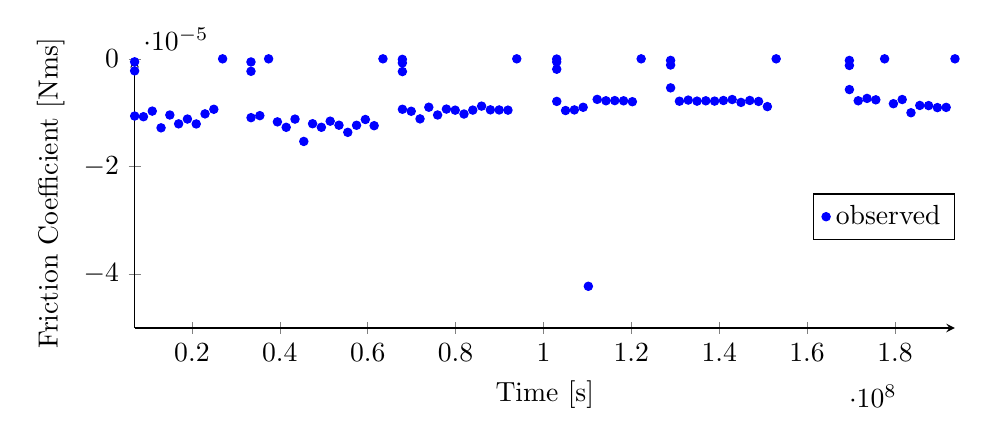
\begin{tikzpicture}
	\begin{axis}[
		height=5cm,
		width=12cm,
		xlabel={Time [s]},
		legend style={at={(1,0.5)}},
		ylabel={Friction Coefficient [Nms]},
		ymin =-5e-5, ymax=0,
		axis x line=bottom,
		axis y line=left,	
]
	\addplot[only marks, mark size=1.5pt, color=blue, mark=*] plot coordinates {
		(6958800, -5.52594650864831e-07)
		(6962400, -2.2311069827034e-06)
		(6969600, -1.06265530730557e-05)
		(8971200, -1.07517197702164e-05)
		(10972800, -9.71169295619254e-06)
		(12974400, -1.28187072721013e-05)
		(14976000, -1.04357030332874e-05)
		(16977600, -1.20777664964105e-05)
		(18979200, -1.11845264927984e-05)
		(20980800, -1.20972510305671e-05)
		(22982400, -1.02243007571275e-05)
		(24984000, -9.37389133279529e-06)
		(26985600, 0.0)
		(33440400, -5.8181412838263e-07)
		(33444000, -2.31766280925503e-06)
		(33451200, -1.09277719757906e-05)
		(35452800, -1.05556707472284e-05)
		(37454400, 0.0)
		(39456000, -1.17095725440834e-05)
		(41457600, -1.27216703287236e-05)
		(43459200, -1.1196277103473e-05)
		(45460800, -1.53468090142071e-05)
		(47462400, -1.2055135669531e-05)
		(49464000, -1.27162982142857e-05)
		(51465600, -1.15806388326882e-05)
		(53467200, -1.2330673316147e-05)
		(55468800, -1.36555430182599e-05)
		(57470400, -1.23428827834912e-05)
		(59472000, -1.12697535858668e-05)
		(61473600, -1.24201760058629e-05)
		(63475200, 0.0)
		(67892400, -9.68316666666667e-08)
		(67896000, -7.63690833333333e-07)
		(67899600, -2.36843486394558e-06)
		(67906800, -9.37002193877551e-06)
		(69908400, -9.74307681099874e-06)
		(71910000, -1.11549130141548e-05)
		(73911600, -8.99001877827569e-06)
		(75913200, -1.04343211452501e-05)
		(77914800, -9.33706241759979e-06)
		(79916400, -9.53711028869707e-06)
		(81918000, -1.02528006121964e-05)
		(83919600, -9.5263653647337e-06)
		(85921200, -8.78581647073413e-06)
		(87922800, -9.47415081979765e-06)
		(89924400, -9.49735194056831e-06)
		(91926000, -9.53405566415816e-06)
		(93927600, 0.0)
		(103017600, -4.16632142857143e-08)
		(103021200, -5.81981826105442e-07)
		(103024800, -1.93184074591009e-06)
		(103032000, -7.90840648252664e-06)
		(105033600, -9.60216933241715e-06)
		(107035200, -9.49074171715562e-06)
		(109036800, -8.99991060454932e-06)
		(110221200, -4.22511030071595e-05)
		(110228400, -0.000175656123782)
		(112230000, -7.53316626247893e-06)
		(114231600, -7.7923449676043e-06)
		(116233200, -7.75991607193652e-06)
		(118234800, -7.79685745372043e-06)
		(120236400, -7.96606077001774e-06)
		(122238000, 0.0)
		(128934000, -2.91303245376276e-07)
		(128937600, -1.14893717873087e-06)
		(128944800, -5.39295703943968e-06)
		(130946400, -7.87617315789917e-06)
		(132948000, -7.66507545600894e-06)
		(134949600, -7.85919358372714e-06)
		(136951200, -7.79847695680762e-06)
		(138952800, -7.85482791350131e-06)
		(140954400, -7.74079487654382e-06)
		(142956000, -7.55788598917364e-06)
		(144957600, -8.09569289396224e-06)
		(146959200, -7.73429548304414e-06)
		(148960800, -7.91533668774021e-06)
		(150962400, -8.87098050790951e-06)
		(152964000, 0.0)
		(169624800, -3.02096696507237e-07)
		(169628400, -1.23172151490436e-06)
		(169635600, -5.71102704908579e-06)
		(171637200, -7.79360262687674e-06)
		(173638800, -7.35464935112867e-06)
		(175640400, -7.61523244318054e-06)
		(177642000, 0.0)
		(179643600, -8.33525638881803e-06)
		(181645200, -7.55823269665951e-06)
		(183646800, -1.00137896663691e-05)
		(185648400, -8.66041035133928e-06)
		(187650000, -8.68942400663265e-06)
		(189651600, -9.05936065452807e-06)
		(191653200, -9.02081130879394e-06)
		(193654800, 0.0)
	};
	\addlegendentry{observed}
	\end{axis}
\end{tikzpicture}

\caption{Friction coefficient observed}
\label{f:rwl_x_observed}
\end{figure}

\begin{figure}[H]
\centering
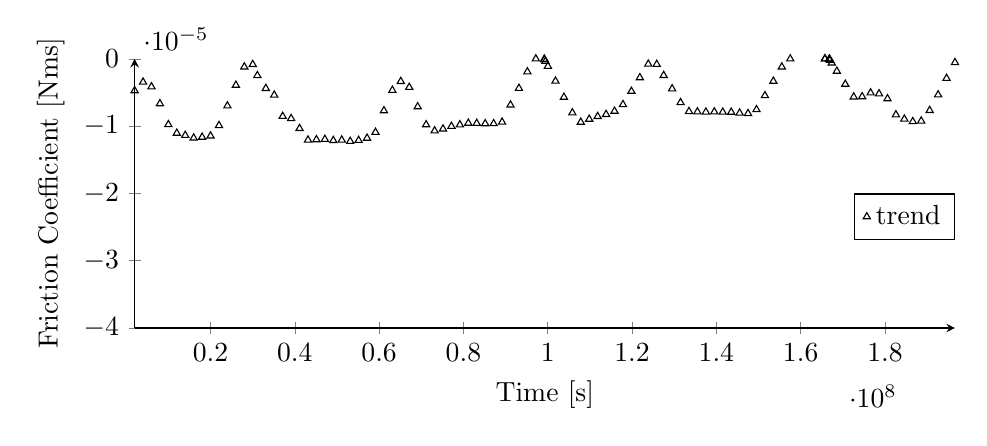
\begin{tikzpicture}
	\begin{axis}[
		height=5cm,
		width=12cm,
		xlabel={Time [s]},
		legend style={at={(1,0.5)}},
		ymin =-4e-5, ymax=0,
		ylabel={Friction Coefficient [Nms]},
		axis x line=bottom,
		axis y line=left,	
]
	\addplot[only marks, mark size=1.5pt, color=black, mark=triangle] plot coordinates {
		(2001600, -4.72498801861756e-06)
		(4003200, -3.45055775713392e-06)
		(6004800, -4.14993643328063e-06)
		(8006400, -6.66696220650753e-06)
		(10008000, -9.77211169066904e-06)
		(12009600, -1.10510292964374e-05)
		(14011200, -1.13665744718071e-05)
		(16012800, -1.17515126757114e-05)
		(18014400, -1.16453834756205e-05)
		(20016000, -1.14578023588243e-05)
		(22017600, -9.90473737340097e-06)
		(24019200, -6.98368838063606e-06)
		(26020800, -3.9155300130534e-06)
		(28022400, -1.19702214749042e-06)
		(30024000, -8.28691009692536e-07)
		(31118400, -2.48662675736359e-06)
		(33120000, -4.3924480445451e-06)
		(35121600, -5.38742034218323e-06)
		(37123200, -8.53764616246858e-06)
		(39124800, -8.8653727392625e-06)
		(41126400, -1.03421027425693e-05)
		(43128000, -1.20629250950313e-05)
		(45129600, -1.20122312692553e-05)
		(47131200, -1.19566177637887e-05)
		(49132800, -1.21288587286924e-05)
		(51134400, -1.20604496600905e-05)
		(53136000, -1.22555424174602e-05)
		(55137600, -1.21128867947182e-05)
		(57139200, -1.1783638780475e-05)
		(59140800, -1.09175099253517e-05)
		(61142400, -7.7018650616502e-06)
		(63144000, -4.67249714544588e-06)
		(65145600, -3.35479095206047e-06)
		(67147200, -4.22913352972679e-06)
		(69148800, -7.11234041282609e-06)
		(71150400, -9.78907928535249e-06)
		(73152000, -1.06960119497206e-05)
		(75153600, -1.04148020193123e-05)
		(77155200, -1.00239171303999e-05)
		(79156800, -9.79716484411886e-06)
		(81158400, -9.55635530517749e-06)
		(83160000, -9.58326229607637e-06)
		(85161600, -9.63060690127688e-06)
		(87163200, -9.6283601084035e-06)
		(89164800, -9.39952243021821e-06)
		(91166400, -6.8569175551947e-06)
		(93168000, -4.37718355234301e-06)
		(95169600, -1.92798680616936e-06)
		(97171200, -2.23086866766565e-21)
		(99172800, -3.95005113899587e-08)
		(99241200, -1.214986227693e-07)
		(99442800, -3.67308015272078e-07)
		(100033200, -1.10193172989548e-06)
		(101833200, -3.30787709462597e-06)
		(103834800, -5.70222786146263e-06)
		(105836400, -8.01657573624419e-06)
		(107838000, -9.41634805729725e-06)
		(109839600, -8.96489766255353e-06)
		(111841200, -8.56670136473909e-06)
		(113842800, -8.25692842725009e-06)
		(115844400, -7.77886280032387e-06)
		(117846000, -6.79136480653098e-06)
		(119847600, -4.8143746481606e-06)
		(121849200, -2.80075854029829e-06)
		(123850800, -7.77613160664722e-07)
		(125852400, -8.19791860991031e-07)
		(127501200, -2.46248660481331e-06)
		(129502800, -4.4468593112889e-06)
		(131504400, -6.50676110521653e-06)
		(133506000, -7.82523001509023e-06)
		(135507600, -7.87747295180367e-06)
		(137509200, -7.90425093377614e-06)
		(139510800, -7.87934890681769e-06)
		(141512400, -7.91791576179654e-06)
		(143514000, -7.92786453164112e-06)
		(145515600, -8.05350658407035e-06)
		(147517200, -8.12936691994529e-06)
		(149518800, -7.54642217212849e-06)
		(151520400, -5.46664224233764e-06)
		(153522000, -3.32190178691765e-06)
		(155523600, -1.19943014047405e-06)
		(157525200, 1.78469493413252e-21)
		(165744000, -1.35405383096579e-09)
		(165751200, -6.209850904982561e-09)
		(166784400, -2.24290534205919e-08)
		(166827600, -6.75189925566516e-08)
		(166960800, -2.02786580004935e-07)
		(167367600, -6.11110402914484e-07)
		(168577200, -1.83608069430413e-06)
		(170578800, -3.76969576476667e-06)
		(172580400, -5.6630530036903e-06)
		(174582000, -5.61705195619934e-06)
		(176583600, -5.05582597600969e-06)
		(178585200, -5.19288950672417e-06)
		(180586800, -5.92624072186377e-06)
		(182588400, -8.30905122662977e-06)
		(184590000, -8.95164435528628e-06)
		(186591600, -9.32130395507415e-06)
		(188593200, -9.23630601340522e-06)
		(190594800, -7.66617846957983e-06)
		(192596400, -5.34832149102885e-06)
		(194598000, -2.89459561351415e-06)
		(196599600, -5.55680490250557e-07)
		(198601200, 1.45006463398267e-21)
	};
	\addlegendentry{trend}
	\end{axis}
\end{tikzpicture}

\caption{Friction coefficient trend}
\label{f:rwl_x_trend}
\end{figure}

\begin{figure}[H]
\centering
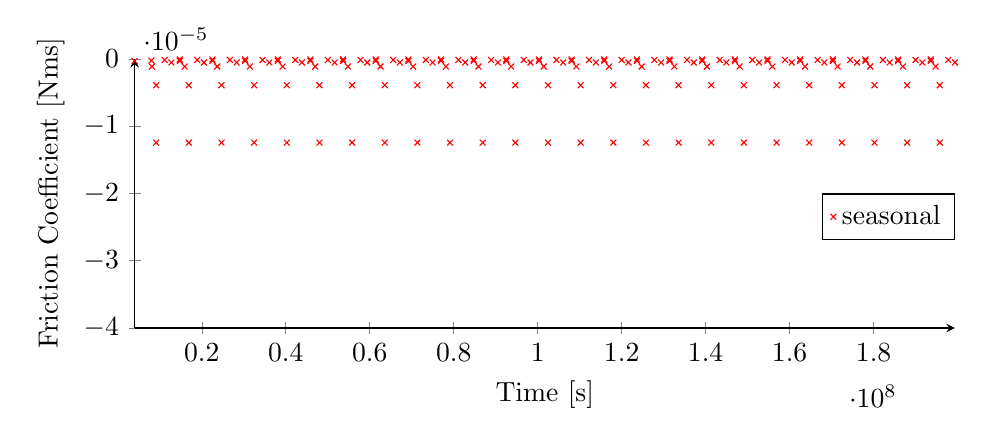
\begin{tikzpicture}
	\begin{axis}[
		height=5cm,
		width=12cm,
		xlabel={Time [s]},
		legend style={at={(1,0.5)}},
		ymin =-4e-5, ymax=0,
		ylabel={Friction Coefficient [Nms]},
		axis x line=bottom,
		axis y line=left,	
]
	\addplot[only marks, mark size=1.5pt, color=red, mark=x] plot coordinates {
		(2001600, 4.5427503484935e-07)
		(4003200, -3.21125334797984e-07)
		(6004800, 2.4850346786433e-07)
		(8006400, -2.45615588950758e-07)
		(8132400, -1.14255662801511e-06)
		(9136800, -3.91702732708128e-06)
		(9144000, -1.24472561895006e-05)
		(11145600, -1.64036466252935e-07)
		(12754800, -5.44695974705143e-07)
		(14756400, -9.8343336118486e-08)
		(14778000, -3.07451133372968e-07)
		(15908400, -1.14255662801511e-06)
		(16912800, -3.91702732708128e-06)
		(16920000, -1.24472561895006e-05)
		(18921600, -1.64036466252935e-07)
		(20530800, -5.44695974705143e-07)
		(22532400, -9.8343336118486e-08)
		(22554000, -3.07451133372968e-07)
		(23684400, -1.14255662801511e-06)
		(24688800, -3.91702732708128e-06)
		(24696000, -1.24472561895006e-05)
		(26697600, -1.64036466252935e-07)
		(28306800, -5.44695974705143e-07)
		(30308400, -9.8343336118486e-08)
		(30330000, -3.07451133372968e-07)
		(31460400, -1.14255662801511e-06)
		(32464800, -3.91702732708128e-06)
		(32472000, -1.24472561895006e-05)
		(34473600, -1.64036466252935e-07)
		(36082800, -5.44695974705143e-07)
		(38084400, -9.8343336118486e-08)
		(38106000, -3.07451133372968e-07)
		(39236400, -1.14255662801511e-06)
		(40240800, -3.91702732708128e-06)
		(40248000, -1.24472561895006e-05)
		(42249600, -1.64036466252935e-07)
		(43858800, -5.44695974705143e-07)
		(45860400, -9.8343336118486e-08)
		(45882000, -3.07451133372968e-07)
		(47012400, -1.14255662801511e-06)
		(48016800, -3.91702732708128e-06)
		(48024000, -1.24472561895006e-05)
		(50025600, -1.64036466252935e-07)
		(51634800, -5.44695974705143e-07)
		(53636400, -9.8343336118486e-08)
		(53658000, -3.07451133372968e-07)
		(54788400, -1.14255662801511e-06)
		(55792800, -3.91702732708128e-06)
		(55800000, -1.24472561895006e-05)
		(57801600, -1.64036466252935e-07)
		(59410800, -5.44695974705143e-07)
		(61412400, -9.8343336118486e-08)
		(61434000, -3.07451133372968e-07)
		(62564400, -1.14255662801511e-06)
		(63568800, -3.91702732708128e-06)
		(63576000, -1.24472561895006e-05)
		(65577600, -1.64036466252935e-07)
		(67186800, -5.44695974705143e-07)
		(69188400, -9.8343336118486e-08)
		(69210000, -3.07451133372968e-07)
		(70340400, -1.14255662801511e-06)
		(71344800, -3.91702732708128e-06)
		(71352000, -1.24472561895006e-05)
		(73353600, -1.64036466252935e-07)
		(74962800, -5.44695974705143e-07)
		(76964400, -9.8343336118486e-08)
		(76986000, -3.07451133372968e-07)
		(78116400, -1.14255662801511e-06)
		(79120800, -3.91702732708128e-06)
		(79128000, -1.24472561895006e-05)
		(81129600, -1.64036466252935e-07)
		(82738800, -5.44695974705143e-07)
		(84740400, -9.8343336118486e-08)
		(84762000, -3.07451133372968e-07)
		(85892400, -1.14255662801511e-06)
		(86896800, -3.91702732708128e-06)
		(86904000, -1.24472561895006e-05)
		(88905600, -1.64036466252935e-07)
		(90514800, -5.44695974705143e-07)
		(92516400, -9.8343336118486e-08)
		(92538000, -3.07451133372968e-07)
		(93668400, -1.14255662801511e-06)
		(94672800, -3.91702732708128e-06)
		(94680000, -1.24472561895006e-05)
		(96681600, -1.64036466252935e-07)
		(98290800, -5.44695974705143e-07)
		(100292400, -9.8343336118486e-08)
		(100314000, -3.07451133372968e-07)
		(101444400, -1.14255662801511e-06)
		(102448800, -3.91702732708128e-06)
		(102456000, -1.24472561895006e-05)
		(104457600, -1.64036466252935e-07)
		(106066800, -5.44695974705143e-07)
		(108068400, -9.8343336118486e-08)
		(108090000, -3.07451133372968e-07)
		(109220400, -1.14255662801511e-06)
		(110224800, -3.91702732708128e-06)
		(110232000, -1.24472561895006e-05)
		(112233600, -1.64036466252935e-07)
		(113842800, -5.44695974705143e-07)
		(115844400, -9.8343336118486e-08)
		(115866000, -3.07451133372968e-07)
		(116996400, -1.14255662801511e-06)
		(118000800, -3.91702732708128e-06)
		(118008000, -1.24472561895006e-05)
		(120009600, -1.64036466252935e-07)
		(121618800, -5.44695974705143e-07)
		(123620400, -9.8343336118486e-08)
		(123642000, -3.07451133372968e-07)
		(124772400, -1.14255662801511e-06)
		(125776800, -3.91702732708128e-06)
		(125784000, -1.24472561895006e-05)
		(127785600, -1.64036466252935e-07)
		(129394800, -5.44695974705143e-07)
		(131396400, -9.8343336118486e-08)
		(131418000, -3.07451133372968e-07)
		(132548400, -1.14255662801511e-06)
		(133552800, -3.91702732708128e-06)
		(133560000, -1.24472561895006e-05)
		(135561600, -1.64036466252935e-07)
		(137170800, -5.44695974705143e-07)
		(139172400, -9.8343336118486e-08)
		(139194000, -3.07451133372968e-07)
		(140324400, -1.14255662801511e-06)
		(141328800, -3.91702732708128e-06)
		(141336000, -1.24472561895006e-05)
		(143337600, -1.64036466252935e-07)
		(144946800, -5.44695974705143e-07)
		(146948400, -9.8343336118486e-08)
		(146970000, -3.07451133372968e-07)
		(148100400, -1.14255662801511e-06)
		(149104800, -3.91702732708128e-06)
		(149112000, -1.24472561895006e-05)
		(151113600, -1.64036466252935e-07)
		(152722800, -5.44695974705143e-07)
		(154724400, -9.8343336118486e-08)
		(154746000, -3.07451133372968e-07)
		(155876400, -1.14255662801511e-06)
		(156880800, -3.91702732708128e-06)
		(156888000, -1.24472561895006e-05)
		(158889600, -1.64036466252935e-07)
		(160498800, -5.44695974705143e-07)
		(162500400, -9.8343336118486e-08)
		(162522000, -3.07451133372968e-07)
		(163652400, -1.14255662801511e-06)
		(164656800, -3.91702732708128e-06)
		(164664000, -1.24472561895006e-05)
		(166665600, -1.64036466252935e-07)
		(168274800, -5.44695974705143e-07)
		(170276400, -9.8343336118486e-08)
		(170298000, -3.07451133372968e-07)
		(171428400, -1.14255662801511e-06)
		(172432800, -3.91702732708128e-06)
		(172440000, -1.24472561895006e-05)
		(174441600, -1.64036466252935e-07)
		(176050800, -5.44695974705143e-07)
		(178052400, -9.8343336118486e-08)
		(178074000, -3.07451133372968e-07)
		(179204400, -1.14255662801511e-06)
		(180208800, -3.91702732708128e-06)
		(180216000, -1.24472561895006e-05)
		(182217600, -1.64036466252935e-07)
		(183826800, -5.44695974705143e-07)
		(185828400, -9.8343336118486e-08)
		(185850000, -3.07451133372968e-07)
		(186980400, -1.14255662801511e-06)
		(187984800, -3.91702732708128e-06)
		(187992000, -1.24472561895006e-05)
		(189993600, -1.64036466252935e-07)
		(191602800, -5.44695974705143e-07)
		(193604400, -9.8343336118486e-08)
		(193626000, -3.07451133372968e-07)
		(194756400, -1.14255662801511e-06)
		(195760800, -3.91702732708128e-06)
		(195768000, -1.24472561895006e-05)
		(197769600, -1.64036466252935e-07)
		(199378800, -5.44695974705143e-07)
	};
	\addlegendentry{seasonal}
	\end{axis}
\end{tikzpicture}

\caption{Friction coefficient seasonal}
\label{f:rwl_x_seasonal}
\end{figure}

\begin{figure}[H]
\centering
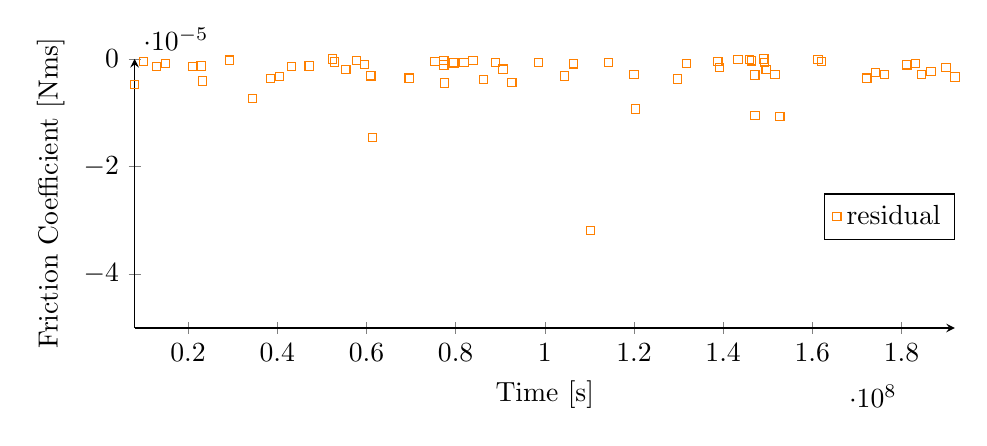
\begin{tikzpicture}
	\begin{axis}[
		height=5cm,
		width=12cm,
		xlabel={Time [s]},
		legend style={at={(1,0.5)}},
		ymin =-5e-5, ymax=0,
		ylabel={Friction Coefficient [Nms]},
		axis x line=bottom,
		axis y line=left,	
]

	\addplot[only marks, mark size=1.5pt, color=orange, mark=square] plot coordinates {
		(2001600, 4.27071298376821e-06)
		(4003200, 3.7716830919319e-06)
		(6004800, 3.9014329654163e-06)
		(8006400, -4.8142384693076e-06)
		(10008000, -4.73427913743276e-07)
		(10872000, 1.42201216878131e-06)
		(12873600, -1.37103083182645e-06)
		(14875200, -8.32072826610267e-07)
		(15429600, 3.90692355253381e-06)
		(16920000, 1.19508087402154e-05)
		(18921600, 5.39517794116458e-07)
		(20923200, -1.4028757592712e-06)
		(22924800, -1.34141674108909e-06)
		(23245200, -4.133511026626e-06)
		(25246800, 4.38749799094964e-06)
		(27248400, 2.44302921387233e-06)
		(29250000, -2.40065086106203e-07)
		(30207600, 7.22947805851576e-07)
		(30639600, 2.17498395308236e-06)
		(32464800, 8.24695225935301e-06)
		(34466400, -7.35987177982831e-06)
		(36468000, 6.80635933134818e-06)
		(38469600, -3.69821174463686e-06)
		(40471200, -3.32285490772361e-06)
		(42472800, 3.56369851839384e-07)
		(43142400, -1.39066161072383e-06)
		(45144000, 1.26778941384546e-06)
		(47145600, -1.34875554862835e-06)
		(48016800, 5.86624619684048e-06)
		(50018400, 2.41689328102461e-07)
		(50364000, 7.36815806807648e-07)
		(52365600, -4.68715678118085e-08)
		(52592400, 1.42106636657909e-07)
		(52880400, -5.81904438415515e-07)
		(54882000, 6.3875709081183e-07)
		(55371600, -1.95519914251813e-06)
		(55800000, 1.1227744610019e-05)
		(57801600, -3.45503080515446e-07)
		(59536800, -1.04788859981643e-06)
		(60976800, -3.16087462639207e-06)
		(61315200, -1.46635133813975e-05)
		(63316800, 4.8417069900293e-06)
		(63576000, 1.64923305041991e-05)
		(65577600, 3.46113877800619e-06)
		(67579200, 4.228695646281e-06)
		(69580800, -3.58541268252813e-06)
		(71352000, 1.17993049793575e-05)
		(73353600, 1.33389712130348e-06)
		(75355200, -5.31013260023026e-07)
		(77356800, -3.17442959888327e-07)
		(77371200, -1.13713771986707e-06)
		(77472000, -4.4897671951203e-06)
		(79473600, 2.44683993108423e-07)
		(79603200, -7.41550988556085e-07)
		(81604800, 2.09156160816703e-07)
		(81878400, -6.43155067985585e-07)
		(83880000, -3.63914205123404e-07)
		(85780800, 1.13622465469181e-06)
		(86306400, -3.79880376661758e-06)
		(86904000, 1.19430900938357e-05)
		(88905600, 1.81809070068513e-07)
		(88959600, -6.38025280475254e-07)
		(90615600, -1.92119260078065e-06)
		(92617200, -4.38460883425714e-06)
		(94618800, 2.9499735046479e-06)
		(94676400, 8.92215226615839e-06)
		(96678000, 2.32743854383002e-07)
		(98643600, -7.08504200419102e-07)
		(100584000, 2.19326377916334e-06)
		(102448800, 7.96654810728257e-06)
		(104450400, -3.17655509005244e-06)
		(106452000, -9.34160003129094e-07)
		(108453600, 1.383871223554e-07)
		(108550800, 4.45600875615e-07)
		(110221200, -3.1900644418734e-05)
		(110224800, -9.58567121248091e-05)
		(110232000, -0.0003179725344677)
		(112233600, 1.12870016816951e-06)
		(114235200, -6.55477127184025e-07)
		(116236800, 2.58773327710672e-07)
		(116996400, 1.11330430052513e-06)
		(118004400, 5.13748300288559e-06)
		(120006000, -2.94006119610915e-06)
		(120387600, -9.33748149836508e-06)
		(122389200, 2.11108494015046e-06)
		(124390800, 2.99112859807424e-07)
		(124772400, 1.14255662801511e-06)
		(125776800, 4.66069594425659e-06)
		(127778400, 2.86802109070241e-06)
		(129780000, -3.73693824091556e-06)
		(131781600, -8.8329381043124e-07)
		(133552800, 3.95128910694839e-06)
		(133560000, 1.24763433974134e-05)
		(135561600, 1.47786413914845e-07)
		(136810800, 4.57030554950139e-07)
		(138812400, -5.20397655009436e-07)
		(139122000, -1.64039822384808e-06)
		(141123600, 5.75311363525802e-07)
		(141328800, 4.01394440175117e-06)
		(141336000, 1.24338288528473e-05)
		(143337600, -1.71457407143579e-07)
		(143946000, 6.39874646833429e-07)
		(145947600, -1.21403865049308e-07)
		(146329200, -3.67488413772989e-07)
		(147117600, -3.00834501623269e-06)
		(147124800, -1.04872869464759e-05)
		(149126400, -4.64818340038828e-08)
		(149144400, 1.53620969002201e-07)
		(149284800, -6.34172556306241e-07)
		(149637600, -1.98925128175828e-06)
		(151639200, -2.86236135259052e-06)
		(152722800, -1.07192240228932e-05)
		(154724400, 2.16182398267263e-06)
		(156726000, 2.87142890892957e-07)
		(156877200, 1.45817554624005e-06)
		(156884400, 6.39162026442993e-06)
		(158886000, 1.47847875673112e-07)
		(159267600, 4.52411195851369e-07)
		(161269200, -1.46312470648193e-07)
		(162115200, -4.66034133503212e-07)
		(164116800, 1.51078562839527e-07)
		(164412000, 5.0863228711505e-07)
		(164656800, 3.91702732708129e-06)
		(164664000, 1.24472561895006e-05)
		(166665600, 1.78298763285115e-07)
		(167000400, 5.39247266121262e-07)
		(168224400, 1.66543998109014e-06)
		(170226000, 2.92667108287525e-06)
		(172227600, -3.59545798332977e-06)
		(174229200, -2.50665978207952e-06)
		(176230800, -2.89062770754786e-06)
		(178232400, 5.33748658510054e-06)
		(179204400, -3.08465788337288e-05)
		(181206000, -1.11619969079259e-06)
		(183207600, -8.95454493984312e-07)
		(184428000, -2.92083413311387e-06)
		(186429600, 7.26846706563687e-07)
		(186606000, -2.32644067298924e-06)
		(187992000, 1.24171521859887e-05)
		(189993600, -1.64354050091067e-06)
		(191995200, -3.37077979196202e-06)
		(193996800, 3.86371530230087e-06)
		(195768000, 1.39703399593146e-05)
		(197769600, 1.64036466252933e-07)
		(199378800, 5.44695974705143e-07)
	};
	\addlegendentry{residual}
	\end{axis}
\end{tikzpicture}

\caption{Friction coefficient residual}
\label{f:rwl_x_residual}
\end{figure}

What can be deduced is a maximum of a possible coefficient, telling something about the health status. With reaction wheel B it can be seen, that the friction increases around $\SI{1e8}{\second}$ ($\approx$ year 2008) where also the increased friction was detected by the operation team. As the wheel is lubricated one year later in 2009, the friction is visibly reduced around $\SI{1.4e8}{\second}$ until all wheels again increase their friction at the end of 2010 before the hibernation.

\subsection{Solar Array}
In figure \ref{f:sag_x_observed} to \ref{f:sag_x_residual} the voltage of the solar array can be seen in its various parts. The trendline in figure \ref{f:sag_x_trend} has a bit more information than the trendline of the reaction wheels. An obvious trend towards a lower voltage can be observed. Unfortunately the seasonal figure \ref{f:sag_x_seasonal} and the noise figure \ref{f:sag_x_residual} don't contain much valuable information.

\begin{figure}[H]
\centering
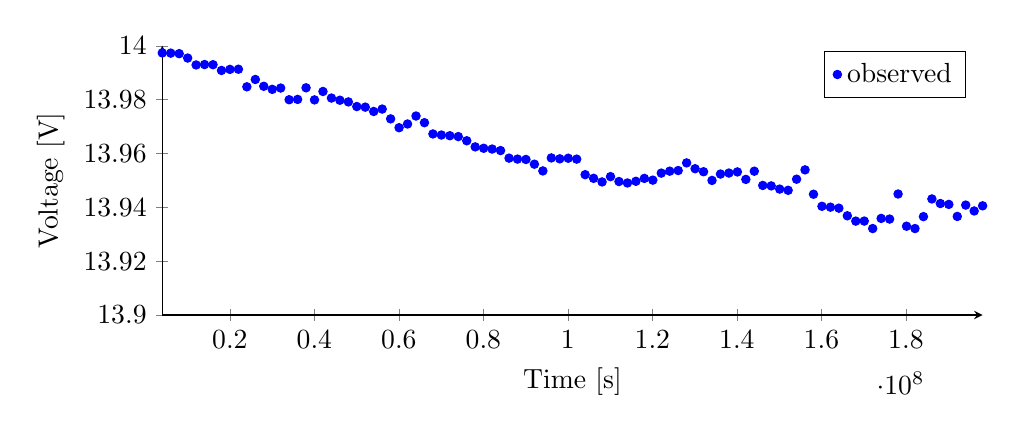
\begin{tikzpicture}
	\begin{axis}[
		height=5cm,
		width=12cm,
		ymin=13.9, ymax=14,
		ylabel={Voltage [V]},
		xlabel={Time [s]},
		axis x line=bottom,
		axis y line=left,
]
	\addplot[only marks, mark size=1.5pt, color=blue, mark=*] plot coordinates {
		(2001600, 14.0011241206506)
		(4003200, 13.9973586769481)
		(6004800, 13.9972819202226)
		(8006400, 13.9970812300231)
		(10008000, 13.9954570522528)
		(12009600, 13.9928879559113)
		(14011200, 13.9930375)
		(16012800, 13.9929827460317)
		(18014400, 13.9908535238868)
		(20016000, 13.9912383346149)
		(22017600, 13.991302479128)
		(24019200, 13.9847696154337)
		(26020800, 13.9874875753711)
		(28022400, 13.9849609005461)
		(30024000, 13.9838281331169)
		(32025600, 13.9843135431924)
		(34027200, 13.9799685679499)
		(36028800, 13.9800917622384)
		(38030400, 13.9843974489796)
		(40032000, 13.9799081419661)
		(42033600, 13.9830329788961)
		(44035200, 13.9805894648757)
		(46036800, 13.9797841755566)
		(48038400, 13.9791598028147)
		(50040000, 13.9774347333024)
		(52041600, 13.9772167659205)
		(54043200, 13.9756047970779)
		(56044800, 13.9764972530759)
		(58046400, 13.9728607154453)
		(60048000, 13.9695731238404)
		(62049600, 13.9709524176716)
		(64051200, 13.9739204081633)
		(66052800, 13.9714387755102)
		(68054400, 13.9672600510204)
		(70056000, 13.9668526750928)
		(72057600, 13.9665989370748)
		(74059200, 13.9662733476345)
		(76060800, 13.9647262760798)
		(78062400, 13.9624523898423)
		(80064000, 13.9619361311761)
		(82065600, 13.9616472418668)
		(84067200, 13.9610833957255)
		(86068800, 13.9582712507323)
		(88070400, 13.9579134273183)
		(90072000, 13.957769850926)
		(92073600, 13.9560179005143)
		(94075200, 13.9535153820021)
		(96076800, 13.9583469387755)
		(98078400, 13.9580137755102)
		(100080000, 13.9582346938776)
		(102081600, 13.9579025510204)
		(104083200, 13.9521251872579)
		(106084800, 13.9507663370887)
		(108086400, 13.9494266320631)
		(110088000, 13.9513961058694)
		(112089600, 13.949581471597)
		(114091200, 13.9490389767031)
		(116092800, 13.9496705374027)
		(118094400, 13.9507496923111)
		(120096000, 13.9500964734686)
		(122097600, 13.9527030612245)
		(124099200, 13.9534270408163)
		(126100800, 13.9536683673469)
		(128102400, 13.9565)
		(130104000, 13.9543439320501)
		(132105600, 13.9532191744174)
		(134107200, 13.9499883679776)
		(136108800, 13.9523557723041)
		(138110400, 13.9527296213138)
		(140112000, 13.9531478410311)
		(142113600, 13.9503722386526)
		(144115200, 13.9534160714286)
		(146116800, 13.9481308767658)
		(148118400, 13.9479575467687)
		(150120000, 13.9467711651898)
		(152121600, 13.946317028285)
		(154123200, 13.9504433673469)
		(156124800, 13.9539096938776)
		(158126400, 13.9448586734694)
		(160128000, 13.9403831632653)
		(162129600, 13.9400540816327)
		(164131200, 13.939681122449)
		(166132800, 13.9368510204082)
		(168134400, 13.9348705708468)
		(170136000, 13.9348899324407)
		(172137600, 13.9321118983945)
		(174139200, 13.9358805774583)
		(176140800, 13.935636312616)
		(178142400, 13.9449464285714)
		(180144000, 13.9329773712894)
		(182145600, 13.9321097866419)
		(184147200, 13.9365453930891)
		(186148800, 13.9431068761596)
		(188150400, 13.9414064076994)
		(190152000, 13.9410806818182)
		(192153600, 13.9366143576067)
		(194155200, 13.9408247506957)
		(196156800, 13.9386446753247)
		(198158400, 13.9405596706865)
	};
	\addlegendentry{observed}
	\end{axis}
\end{tikzpicture}

\caption{Solar array voltage observed}
\label{f:sag_x_observed}
\end{figure}

\begin{figure}[H]
\centering
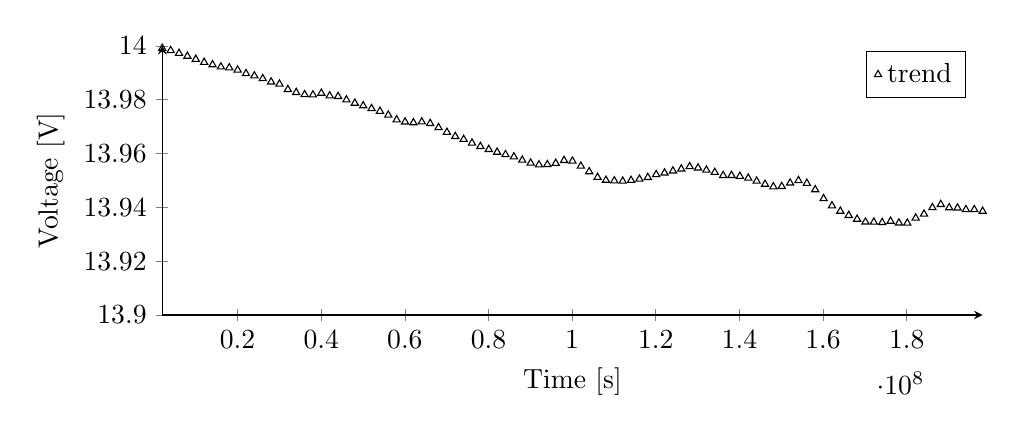
\begin{tikzpicture}
	\begin{axis}[
		height=5cm,
		width=12cm,
		ymin=13.9, ymax=14,
		ylabel={Voltage [V]},
		xlabel={Time [s]},
		axis x line=bottom,
		axis y line=left,
]
	\addplot[only marks, mark size=1.5pt, color=black, mark=triangle] plot coordinates {
		(2001600, 13.9990904074361)
		(4003200, 13.9982520753059)
		(6004800, 13.9972152940887)
		(8006400, 13.9961348212631)
		(10008000, 13.9950095234671)
		(12009600, 13.9938652358022)
		(14011200, 13.9929820055538)
		(16012800, 13.992185058904)
		(18014400, 13.9918528133856)
		(20016000, 13.9910112080457)
		(22017600, 13.9896853805001)
		(24019200, 13.988849435601)
		(26020800, 13.987826405803)
		(28022400, 13.986586476811)
		(30024000, 13.9857922253671)
		(32025600, 13.9837821781912)
		(34027200, 13.9826699867777)
		(36028800, 13.9818732184259)
		(38030400, 13.9817772698917)
		(40032000, 13.9823852309516)
		(42033600, 13.9814451227277)
		(44035200, 13.9812071686888)
		(46036800, 13.9799239263221)
		(48038400, 13.9787015485582)
		(50040000, 13.9777417447431)
		(52041600, 13.9766993060282)
		(54043200, 13.9756911052518)
		(56044800, 13.974290612114)
		(58046400, 13.972534477257)
		(60048000, 13.9717252685433)
		(62049600, 13.9714357785378)
		(64051200, 13.9717424522896)
		(66052800, 13.9711700091431)
		(68054400, 13.969629624341)
		(70056000, 13.9678854703414)
		(72057600, 13.9663295351849)
		(74059200, 13.9652639703007)
		(76060800, 13.9638899303406)
		(78062400, 13.9626167220906)
		(80064000, 13.9615241486839)
		(82065600, 13.9604860622168)
		(84067200, 13.9595822665802)
		(86068800, 13.9587770941505)
		(88070400, 13.9575343191199)
		(90072000, 13.9564541701242)
		(92073600, 13.9558019198582)
		(94075200, 13.955883982676)
		(96076800, 13.9563706142742)
		(98078400, 13.9574201514355)
		(100080000, 13.9571873811772)
		(102081600, 13.9553076832612)
		(104083200, 13.9532334236263)
		(106084800, 13.9511252435519)
		(108086400, 13.9500707019201)
		(110088000, 13.9498563688331)
		(112089600, 13.9497351363257)
		(114091200, 13.9500144524589)
		(116092800, 13.9504934146568)
		(118094400, 13.9511060224579)
		(120096000, 13.9521706975505)
		(122097600, 13.95277366739)
		(124099200, 13.9535228720223)
		(126100800, 13.9542494841819)
		(128102400, 13.9551239158228)
		(130104000, 13.9546490240558)
		(132105600, 13.9538281527076)
		(134107200, 13.9529935391455)
		(136108800, 13.9518227471939)
		(138110400, 13.9518659408145)
		(140112000, 13.951540158834)
		(142113600, 13.9508472617683)
		(144115200, 13.9497488518944)
		(146116800, 13.9485787888322)
		(148118400, 13.9476443404845)
		(150120000, 13.9477472481564)
		(152121600, 13.9490473348513)
		(154123200, 13.9499445312148)
		(156124800, 13.9489454588257)
		(158126400, 13.9465454717341)
		(160128000, 13.9432560834751)
		(162129600, 13.940577303595)
		(164131200, 13.9385671341286)
		(166132800, 13.9370031445871)
		(168134400, 13.935595654471)
		(170136000, 13.9345522101534)
		(172137600, 13.9345212084853)
		(174139200, 13.9343682076531)
		(176140800, 13.9348430539115)
		(178142400, 13.9342036330144)
		(180144000, 13.9341345695728)
		(182145600, 13.9360326214552)
		(184147200, 13.9374889053569)
		(186148800, 13.9398897117573)
		(188150400, 13.9410681266598)
		(190152000, 13.9398473335696)
		(192153600, 13.939758808704)
		(194155200, 13.9391586017412)
		(196156800, 13.9391708901972)
		(198158400, 13.9385549743603)
	};
	\addlegendentry{trend}
	\end{axis}
\end{tikzpicture}

\caption{Solar array voltage trend}
\label{f:sag_x_trend}
\end{figure}

\begin{figure}[H]
\centering
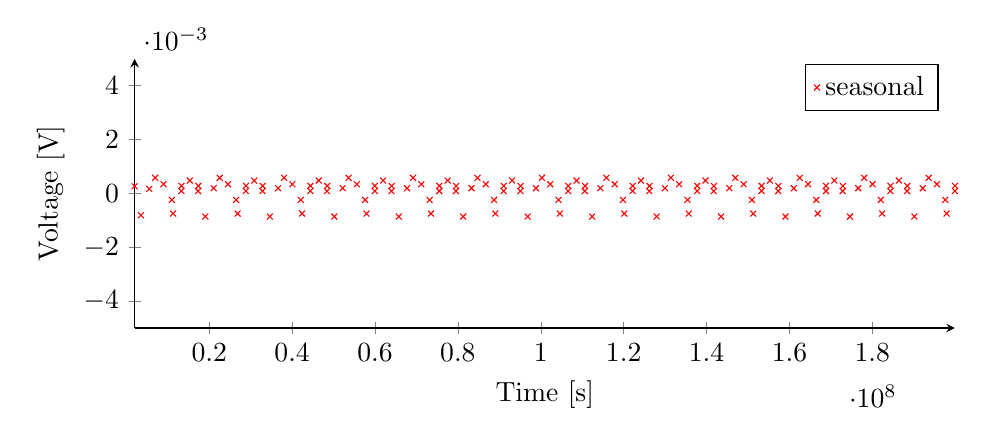
\begin{tikzpicture}
	\begin{axis}[
		height=5cm,
		width=12cm,
		ymin=-0.005, ymax=0.005,
		ylabel={Voltage [V]},
		xlabel={Time [s]},
		axis x line=bottom,
		axis y line=left,
]
	\addplot[only marks, mark size=1.5pt, color=red, mark=x] plot coordinates {
		(2001600, 0.000263953508996)
		(3520800, -0.0008118075527883)
		(5522400, 0.0001693329396408)
		(6969600, 0.0005795766344836)
		(8971200, 0.0003416510514417)
		(10972800, -0.0002418027490826)
		(11293200, -0.000748740609779)
		(13294800, 8.95985533127747e-05)
		(13312800, 0.0002808770440608)
		(15314400, 0.0004781697630149)
		(17316000, 8.63024521693762e-05)
		(17362800, 0.0002760287301625)
		(19076400, -0.0008593963666597)
		(21078000, 0.0001907588672345)
		(22521600, 0.0005795766344836)
		(24523200, 0.0003416510514417)
		(26524800, -0.0002418027490826)
		(26845200, -0.000748740609779)
		(28846800, 8.95985533127747e-05)
		(28864800, 0.0002808770440608)
		(30866400, 0.0004781697630149)
		(32868000, 8.63024521693762e-05)
		(32914800, 0.0002760287301625)
		(34628400, -0.0008593963666597)
		(36630000, 0.0001907588672345)
		(38073600, 0.0005795766344836)
		(40075200, 0.0003416510514417)
		(42076800, -0.0002418027490826)
		(42397200, -0.000748740609779)
		(44398800, 8.95985533127747e-05)
		(44416800, 0.0002808770440608)
		(46418400, 0.0004781697630149)
		(48420000, 8.63024521693762e-05)
		(48466800, 0.0002760287301625)
		(50180400, -0.0008593963666597)
		(52182000, 0.0001907588672345)
		(53625600, 0.0005795766344836)
		(55627200, 0.0003416510514417)
		(57628800, -0.0002418027490826)
		(57949200, -0.000748740609779)
		(59950800, 8.95985533127747e-05)
		(59968800, 0.0002808770440608)
		(61970400, 0.0004781697630149)
		(63972000, 8.63024521693762e-05)
		(64018800, 0.0002760287301625)
		(65732400, -0.0008593963666597)
		(67734000, 0.0001907588672345)
		(69177600, 0.0005795766344836)
		(71179200, 0.0003416510514417)
		(73180800, -0.0002418027490826)
		(73501200, -0.000748740609779)
		(75502800, 8.95985533127747e-05)
		(75520800, 0.0002808770440608)
		(77522400, 0.0004781697630149)
		(79524000, 8.63024521693762e-05)
		(79570800, 0.0002760287301625)
		(81284400, -0.0008593963666597)
		(83286000, 0.0001907588672345)
		(84729600, 0.0005795766344836)
		(86731200, 0.0003416510514417)
		(88732800, -0.0002418027490826)
		(89053200, -0.000748740609779)
		(91054800, 8.95985533127747e-05)
		(91072800, 0.0002808770440608)
		(93074400, 0.0004781697630149)
		(95076000, 8.63024521693762e-05)
		(95122800, 0.0002760287301625)
		(96836400, -0.0008593963666597)
		(98838000, 0.0001907588672345)
		(100281600, 0.0005795766344836)
		(102283200, 0.0003416510514417)
		(104284800, -0.0002418027490826)
		(104605200, -0.000748740609779)
		(106606800, 8.95985533127747e-05)
		(106624800, 0.0002808770440608)
		(108626400, 0.0004781697630149)
		(110628000, 8.63024521693762e-05)
		(110674800, 0.0002760287301625)
		(112388400, -0.0008593963666597)
		(114390000, 0.0001907588672345)
		(115833600, 0.0005795766344836)
		(117835200, 0.0003416510514417)
		(119836800, -0.0002418027490826)
		(120157200, -0.000748740609779)
		(122158800, 8.95985533127747e-05)
		(122176800, 0.0002808770440608)
		(124178400, 0.0004781697630149)
		(126180000, 8.63024521693762e-05)
		(126226800, 0.0002760287301625)
		(127940400, -0.0008593963666597)
		(129942000, 0.0001907588672345)
		(131385600, 0.0005795766344836)
		(133387200, 0.0003416510514417)
		(135388800, -0.0002418027490826)
		(135709200, -0.000748740609779)
		(137710800, 8.95985533127747e-05)
		(137728800, 0.0002808770440608)
		(139730400, 0.0004781697630149)
		(141732000, 8.63024521693762e-05)
		(141778800, 0.0002760287301625)
		(143492400, -0.0008593963666597)
		(145494000, 0.0001907588672345)
		(146937600, 0.0005795766344836)
		(148939200, 0.0003416510514417)
		(150940800, -0.0002418027490826)
		(151261200, -0.000748740609779)
		(153262800, 8.95985533127747e-05)
		(153280800, 0.0002808770440608)
		(155282400, 0.0004781697630149)
		(157284000, 8.63024521693762e-05)
		(157330800, 0.0002760287301625)
		(159044400, -0.0008593963666597)
		(161046000, 0.0001907588672345)
		(162489600, 0.0005795766344836)
		(164491200, 0.0003416510514417)
		(166492800, -0.0002418027490826)
		(166813200, -0.000748740609779)
		(168814800, 8.95985533127747e-05)
		(168832800, 0.0002808770440608)
		(170834400, 0.0004781697630149)
		(172836000, 8.63024521693762e-05)
		(172882800, 0.0002760287301625)
		(174596400, -0.0008593963666597)
		(176598000, 0.0001907588672345)
		(178041600, 0.0005795766344836)
		(180043200, 0.0003416510514417)
		(182044800, -0.0002418027490826)
		(182365200, -0.000748740609779)
		(184366800, 8.95985533127747e-05)
		(184384800, 0.0002808770440608)
		(186386400, 0.0004781697630149)
		(188388000, 8.63024521693762e-05)
		(188434800, 0.0002760287301625)
		(190148400, -0.0008593963666597)
		(192150000, 0.0001907588672345)
		(193593600, 0.0005795766344836)
		(195595200, 0.0003416510514417)
		(197596800, -0.0002418027490826)
		(197917200, -0.000748740609779)
		(199918800, 8.95985533127747e-05)
		(199936800, 0.0002808770440608)
	};
	\addlegendentry{seasonal}
	\end{axis}
\end{tikzpicture}

\caption{Solar array voltage seasonal}
\label{f:sag_x_seasonal}
\end{figure}

\begin{figure}[H]
\centering
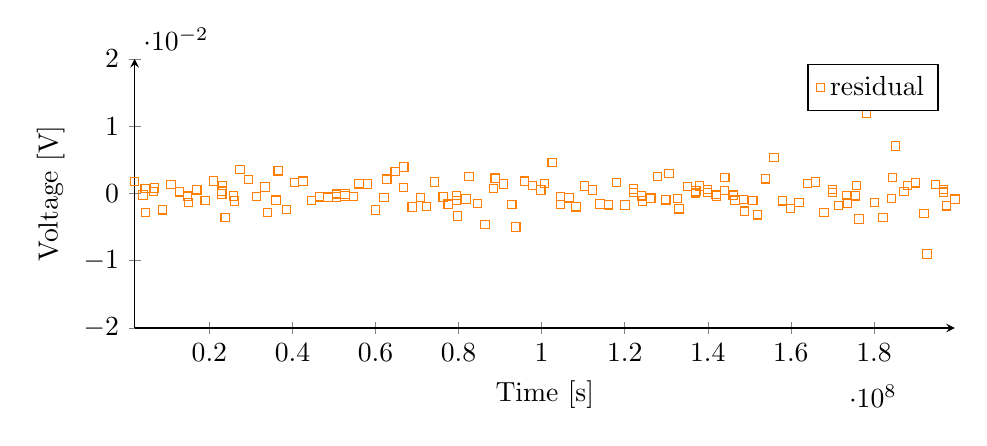
\begin{tikzpicture}
	\begin{axis}[
		height=5cm,
		width=12cm,
		ymin=-0.02, ymax=0.02,
		ylabel={Voltage [V]},
		xlabel={Time [s]},
		axis x line=bottom,
		axis y line=left,
]
	\addplot[only marks, mark size=1.5pt, color=orange, mark=square] plot coordinates {
		(2001600, 0.0017697597055624)
		(4003200, -0.0002267475155595)
		(4532400, 0.0007004000393119)
		(4554000, -0.0027933339381932)
		(6555600, 0.0002559988123704)
		(6775200, 0.0008131812475184)
		(8740800, -0.0024475684620973)
		(10742400, 0.0013480221619961)
		(12744000, 0.0002307862232037)
		(14745600, -0.0003994085636123)
		(14986800, -0.0013731202368627)
		(16988400, 0.0005376606716135)
		(18990000, -0.0010183930019703)
		(20991600, 0.0018337638991467)
		(22993200, -9.63826160294034e-05)
		(23018400, 0.0003390978249754)
		(23140800, 0.0011616539419552)
		(23803200, -0.0035519178659143)
		(25804800, -0.0003723630016032)
		(26100000, -0.0011305612386669)
		(27370800, 0.0035532118888368)
		(29372400, 0.0020843397005794)
		(31374000, -0.0004963459059234)
		(33375600, 0.0009497602315774)
		(34052400, -0.0028747056608796)
		(36054000, -0.0009968873168844)
		(36554400, 0.003356317731096)
		(38556000, -0.002383783875318)
		(40557600, 0.001638664027274)
		(42559200, 0.0018224479323117)
		(44560800, -0.0010820602523716)
		(46562400, -0.0005153908955486)
		(48564000, -0.0005507871737898)
		(50565600, 2.91754290089944e-05)
		(50569200, -0.0001516449908787)
		(50659200, -0.0005371294432834)
		(52660800, -9.77092608228309e-05)
		(52671600, -0.0003807415613144)
		(54673200, -0.0004711197130712)
		(56023200, 0.001427620810797)
		(58024800, 0.001395445532766)
		(60026400, -0.0024537007730928)
		(62028000, -0.0006482017770883)
		(62733600, 0.0021168458320665)
		(64735200, 0.0032145438197363)
		(66736800, 0.0009079324279487)
		(66812400, 0.003929968622954)
		(68814000, -0.0020165704678793)
		(70815600, -0.0006372722354387)
		(72270000, -0.0019533138612821)
		(74271600, 0.0017057838900933)
		(76273200, -0.0005200891098558)
		(77479200, -0.0015945102042988)
		(79480800, -0.0003096502921771)
		(79542000, -0.001070236948838)
		(79776000, -0.003356509069077)
		(81777600, -0.0008438550557387)
		(82508400, 0.0025558018945748)
		(84510000, -0.0014772234474436)
		(86374800, -0.0045781033697558)
		(88376400, 0.0007304249471529)
		(88808400, 0.0022708184143694)
		(90810000, 0.0014059052113766)
		(92811600, -0.001606768727453)
		(93798000, -0.0050000626679828)
		(95799600, 0.0018255316794751)
		(97801200, 0.0011553925313428)
		(99802800, 0.0004937127320709)
		(100706400, 0.0015001378753629)
		(102520800, 0.0045561945601808)
		(104522400, -0.0004694037114404)
		(104587200, -0.001627793490144)
		(106588800, -0.0006634548717095)
		(108259200, -0.0019996062692231)
		(110260800, 0.0011147179805261)
		(112262400, 0.0005096341986819)
		(114044400, -0.0015642633240527)
		(116046000, -0.0017028976899804)
		(118047600, 0.0015827836249347)
		(120049200, -0.0017163716051323)
		(122050800, 0.0001700563881872)
		(122058000, 0.0006674767115896)
		(124059600, -0.0003578751211965)
		(124290000, -0.0011201776130268)
		(126291600, -0.0007025216962819)
		(127897200, 0.0024776534810708)
		(129898800, -0.0009540714890052)
		(130665600, 0.0029678308289611)
		(132667200, -0.0007186380900844)
		(133052400, -0.0022894963058602)
		(135054000, 0.0009982967672645)
		(137055600, 2.4722130542676e-05)
		(137059200, 0.0001062965845793)
		(137109600, 0.0003524706003357)
		(137948400, 0.001090417470252)
		(139950000, 0.0001793361712025)
		(139978800, 0.0006095514855166)
		(141980400, -0.000125074593888)
		(142077600, -0.0003904604450214)
		(144079200, 0.0004592050184378)
		(144108000, 0.0023447213371609)
		(146109600, -0.0002535050571297)
		(146556000, -0.0009934644010226)
		(148557600, -0.0008644933038692)
		(148842000, -0.0026302243643079)
		(150843600, -0.0010620614432668)
		(151945200, -0.003188316116845)
		(153946800, 0.0021581346264056)
		(155948400, 0.0053215838257016)
		(157950000, -0.0010991974354555)
		(159951600, -0.0022726116440178)
		(161953200, -0.0013737747306857)
		(163954800, 0.0014807722929081)
		(165956400, 0.0016879504130095)
		(167958000, -0.0028215101124902)
		(169959600, 0.0001590111698839)
		(170082000, 0.0005489302992118)
		(171482400, -0.0018212360036003)
		(173484000, -0.0003145756534491)
		(173592000, -0.001416886837279)
		(175593600, -0.0003687144945314)
		(175845600, 0.0011359014065316)
		(176396400, -0.0038106148557573)
		(178178400, 0.0118701796985925)
		(180180000, -0.0013908262228047)
		(182181600, -0.0036203872383715)
		(184183200, -0.0007461444865732)
		(184442400, 0.0023267352255294)
		(185227200, 0.0070544012408114)
		(187228800, 0.0002540833071258)
		(188031600, 0.0011334234542613)
		(190033200, 0.0015777086453302)
		(192034800, -0.002979649465903)
		(192780000, -0.009002005045954)
		(194781600, 0.0012970175153423)
		(196783200, 0.0001829513924783)
		(196797600, 0.0005723736632011)
		(197506800, -0.0018452326474628)
		(199508400, -0.0008539743623834)
	};
	\addlegendentry{residual}
	\end{axis}
\end{tikzpicture}

\caption{Solar array voltage residual}
\label{f:sag_x_residual}
\end{figure}

\section{Conclusion}
The chapter about data-mining did show general features of the used dataset with basic statistical methods. It was seen for the Rosetta Housekeeping data, that datapoints were measured in unequal timesteps and had to be interpolated to get a common samplerate / periodicity. The next step was to find interesting frequencies for later analysis, but this proved to be difficult as there was no specific oscillation or seasonality. Only the magnitude over the whole spectrum gave some indications of differences between the four reaction wheels.
Following this, the X11-method for trend and seasonality analysis didn't find much more information in the datasets. Neither for the reaction wheels nor for the solar array, even though the solar array performance follows a decreasing trend. This might be due to the effect, that this data still does not include any seasons and the window size might have been chosen much larger to represent and extrapolate the decreasing trend accordingly.